% content_body_en.tex
% English counterpart of content_body.tex. Shared document content for all
% editions of the English book (main_en.tex, main_kdp_print_en.tex,
% main_bod_print_en.tex). Make changes to chapter order, preface, or
% backmatter HERE only, not in the wrapper files.
%
% Expects the wrapper to optionally define \editionimpressum before
% % content_body_en.tex
% English counterpart of content_body.tex. Shared document content for all
% editions of the English book (main_en.tex, main_kdp_print_en.tex,
% main_bod_print_en.tex). Make changes to chapter order, preface, or
% backmatter HERE only, not in the wrapper files.
%
% Expects the wrapper to optionally define \editionimpressum before
% % content_body_en.tex
% English counterpart of content_body.tex. Shared document content for all
% editions of the English book (main_en.tex, main_kdp_print_en.tex,
% main_bod_print_en.tex). Make changes to chapter order, preface, or
% backmatter HERE only, not in the wrapper files.
%
% Expects the wrapper to optionally define \editionimpressum before
% % content_body_en.tex
% English counterpart of content_body.tex. Shared document content for all
% editions of the English book (main_en.tex, main_kdp_print_en.tex,
% main_bod_print_en.tex). Make changes to chapter order, preface, or
% backmatter HERE only, not in the wrapper files.
%
% Expects the wrapper to optionally define \editionimpressum before
% \input{content_body_en} (the imprint/ISBN text for that edition). If
% \editionimpressum is not defined, a TODO placeholder is printed.

\providecommand{\editionimpressum}{%
    \textbf{TODO: add imprint/ISBN for this edition.}\\[1em]
    \textcopyright\ Wolfgang Becker\\
    All rights reserved.
}

\frontmatter
\maketitle

\cleardoublepage
\thispagestyle{empty}
\vspace*{\fill}
\noindent
\editionimpressum
\vspace*{\fill}
\clearpage

\tableofcontents

\chapter*{Preface}
This textbook is for beginners with no prior knowledge of SysML v2, MBSE, or ROS2.
The goal is not to cover every special case of modeling theory. The goal is to build a working understanding:
What is a system model? How do you describe requirements? How does an architecture grow from them? And how do you map that architecture onto a ROS2 robotics system?

The book uses one example throughout: an autonomous indoor robot. The robot must detect obstacles, map rooms, drive to target positions, recognize people, and monitor its battery level.
The example is small enough for a beginner, but realistic enough to show the key ideas of Model-Based Systems Engineering.

The Syside Editor checked all SysML v2 code examples in this book (version 0.10.2, checked on 2026-07-07). SysML v2 and its tools are still under active development. Different tool versions may therefore show small syntax differences, for example in how you write \texttt{verify ... by}. If you are unsure, check code examples against your installed tool version.

\mainmatter

\input{chapters_en/01_systems_engineering}
\input{chapters_en/02_mbse}
\input{chapters_en/03_sysml_grundlagen}
\input{chapters_en/04_sysml_v2_werkzeuge}
\input{chapters_en/05_praxisprojekt}
\input{chapters_en/06_anforderungen}
\input{chapters_en/07_stakeholder_use_cases}
\input{chapters_en/08_bdd}
\input{chapters_en/09_ibd}
\input{chapters_en/10_schnittstellen}
\input{chapters_en/11_activity_diagrams}
\input{chapters_en/12_state_machines}
\input{chapters_en/13_parametrik}
\input{chapters_en/14_ros2_grundlagen}
\input{chapters_en/15_ros2_architektur}
\input{chapters_en/16_sysml_ros2_mapping}
\input{chapters_en/17_ros2_python}
\input{chapters_en/18_ml_integration}
\input{chapters_en/19_tests_verifikation}
\input{chapters_en/20_traceability}
\input{chapters_en/21_abschlussprojekt}
\input{chapters_en/22_ausblick}

\backmatter
\glsaddall
\printglossary[type=\acronymtype,title=List of Abbreviations]
\printglossary[title=Glossary]
\bibliographystyle{plain}
\bibliography{references_en}

\listoffigures

\printindex
 (the imprint/ISBN text for that edition). If
% \editionimpressum is not defined, a TODO placeholder is printed.

\providecommand{\editionimpressum}{%
    \textbf{TODO: add imprint/ISBN for this edition.}\\[1em]
    \textcopyright\ Wolfgang Becker\\
    All rights reserved.
}

\frontmatter
\maketitle

\cleardoublepage
\thispagestyle{empty}
\vspace*{\fill}
\noindent
\editionimpressum
\vspace*{\fill}
\clearpage

\tableofcontents

\chapter*{Preface}
This textbook is for beginners with no prior knowledge of SysML v2, MBSE, or ROS2.
The goal is not to cover every special case of modeling theory. The goal is to build a working understanding:
What is a system model? How do you describe requirements? How does an architecture grow from them? And how do you map that architecture onto a ROS2 robotics system?

The book uses one example throughout: an autonomous indoor robot. The robot must detect obstacles, map rooms, drive to target positions, recognize people, and monitor its battery level.
The example is small enough for a beginner, but realistic enough to show the key ideas of Model-Based Systems Engineering.

The Syside Editor checked all SysML v2 code examples in this book (version 0.10.2, checked on 2026-07-07). SysML v2 and its tools are still under active development. Different tool versions may therefore show small syntax differences, for example in how you write \texttt{verify ... by}. If you are unsure, check code examples against your installed tool version.

\mainmatter

\chapter{Understanding Systems Engineering}

\begin{lernziele}
This chapter explains what a system is and why systems engineering is necessary for complex technical products. You will understand the difference between a single component and the behavior of a system. You will learn to name stakeholders (people, groups, or organizations with an interest in the system), draw a system boundary, and recognize typical beginner mistakes. Using an autonomous indoor robot as an example, you will practice thinking in terms of requirements, functions, interfaces, and verification.
\end{lernziele}

\section{Introduction}
Many technical projects start with a simple idea. Someone says: \enquote{We will build a robot that drives through a building on its own.} At first, that sounds manageable. The robot needs wheels, motors, sensors, a computer, some software, and a battery. Once the parts are available, the project should mainly consist of construction, programming, and testing.

In practice, this view turns out to be too simple. An autonomous indoor robot must not just drive. It must drive safely. It must detect obstacles, avoid endangering people, handle doors and narrow corridors, monitor its battery level, return to its charging station when needed, and stay easy for users to operate. At the same time, it must stay affordable, remain maintainable, and fit into a real environment. Even this small example already combines mechanics, electronics, software, artificial intelligence, power supply, safety considerations, operating concepts, and organizational questions.

This is exactly where systems engineering begins. Systems engineering is a way of working for developing complex systems. It helps a team think from the problem outward, instead of jumping to individual solutions too early. It asks:

\begin{itemize}
    \item Which problem needs to be solved?
    \item Who has expectations of the system?
    \item What belongs to the system, and what belongs to its environment?
    \item Which functions must the system provide?
    \item Which requirements must the system meet, in a way we can check?
    \item Which components, interfaces, and sequences does this require?
    \item How do we prove that the finished system really works?
\end{itemize}

For beginners, one point matters most: systems engineering is not extra bureaucracy that makes a project artificially harder. Used well, it creates clarity. It stops a team from jumping into details too early and discovering later that important expectations were overlooked. In this textbook, we use systems engineering as a way of thinking. We do not want to memorize every standard. We want to understand how to describe a technical system clearly, structure it, and turn it step by step into a workable architecture.

\section{What Is a System?}
A system is a set of elements that work together to serve a purpose. This definition sounds simple, but it makes three important points.

First, a system consists of several elements. For the indoor robot, these are, for example, sensors, a computer, software components, a battery, motors, wheels, a housing, charging contacts, and user interfaces. People, too, can belong to a system in a broader sense -- for example, operators, maintenance staff, or people in the robot's driving area.

Second, these elements work together. A single lidar sensor (a sensor that measures distance with a laser) does not by itself make an autonomous robot. The desired behavior only appears once the sensor delivers measurement data, software processes that data and builds a map from it, navigation plans a path, and the motor controller executes matching drive commands.

Third, a system has a purpose. The purpose of our robot could be: \enquote{The robot transports small items on its own inside an office building.} A different purpose would be: \enquote{The robot monitors corridors at night and reports unusual events.} Both systems might look similar on the outside, but they would have different requirements, different stakeholders, and different technical priorities.

\begin{praxisbox}
Picture two robots with similar hardware. The first robot transports medication in a hospital. The second robot delivers tools in a workshop. Both need navigation and obstacle detection. Even so, their requirements differ sharply. In the hospital, hygiene, quiet operation, patient safety, and reliable documentation matter most. In the workshop, ruggedness, dust protection, and safe movement between machines matter most. A system is therefore defined not just by its parts, but by its purpose and its operating environment.
\end{praxisbox}

\subsection{Elements, Relationships, and Behavior}
A common beginner mistake is to treat a system as nothing more than a list of parts:

\begin{itemize}
    \item camera
    \item lidar
    \item battery
    \item motor controller
    \item computer
    \item ROS2 software (a robotics software platform, see chapter 14)
\end{itemize}

This list is useful, but it is not enough. What matters is the relationships between the parts. The camera sends images to recognition software. The recognition software reports detected people to navigation. Navigation takes obstacles into account and produces target speeds. The motor controller turns these target speeds into electrical signals for the motors. The battery monitor reports a low charge level, which triggers mission planning to start a return to the charging station.

System behavior, then, grows out of this interplay. Engineers often call this emergent behavior: the behavior of the whole system is more than the sum of its parts. A motor can turn, a sensor can measure, and a computer can run programs. Autonomous navigation, however, only appears once these abilities are connected in a meaningful way.

\subsection{Open and Closed Systems}
Many technical systems are open systems. They constantly exchange something with their environment. The indoor robot senses its environment through sensors, puts movement into that environment, draws energy from the charging station, and may communicate with users or a building management system.

This matters because engineers cannot fully understand open systems in a lab. A robot that works well in a test hall can run into trouble in a real office building: reflective glass surfaces, narrow passages, changing light, people with rolling suitcases, open doors, carpet edges, or Wi-Fi dropouts. Systems engineering therefore forces us to think about the environment early on.

\section{Why Systems Engineering?}
In small projects, a team can often just start building. Someone writing a simple Python script can keep requirements, design, implementation, and testing in their head at once. This stops working reliably once a product grows more complex. Too many decisions depend on each other.

Suppose a team decides to use a stronger camera so it can recognize people better. This change sounds local. In reality, it can have many consequences:

\begin{itemize}
    \item The camera produces more data.
    \item The computer needs more processing power.
    \item The software must process larger images faster.
    \item Power consumption rises.
    \item The battery lasts less time.
    \item The housing may need a different mount.
    \item Heat buildup may increase.
    \item The price of the robot rises.
\end{itemize}

Systems engineering helps make such dependencies visible. It looks not just at one component, but at the whole system and its life cycle: idea, requirements, design, implementation, integration, test, operation, maintenance, and later evolution.

\subsection{Making Complexity Manageable}
Complexity does not just mean that a system has many parts. A system becomes complex mainly through many interactions, unclear expectations, and changes during development. A robot project becomes complex because hardware, software, and environment all play a role at the same time.

Here is an example. Navigation should choose the shortest path. The safety requirement, however, says that the robot must slow down near people. The battery requirement says that the robot must return to the charging station in time. The user requirement says that deliveries must not take too long. These requirements can conflict with each other. Systems engineering makes such conflicts visible before they only show up once someone tests the finished robot.

\subsection{Improving Communication}
Technical projects are teamwork. Mechanical engineering, electronics, software, testing, project management, purchasing, operations, and the customer side often use different terms. What a software developer calls a \enquote{node} may, to a systems engineer, be a functional unit. The development team must translate what a user calls \enquote{fast} into measurable requirements.

Systems engineering creates shared descriptions. These descriptions can be texts, tables, diagrams, and models. Later in this book, we use SysML for this. At first, though, the point is the way of thinking: we want to clarify terms, make connections visible, and document decisions so that others can follow them.

\subsection{Finding Errors Earlier}
The later an error is found, the more expensive it becomes to fix. If a team only realizes shortly before delivery that the battery is too small for the planned drive time, it may need to change the housing, re-evaluate the center of gravity, and adjust the charging electronics. If this question is examined early, through requirements and simple calculations, the fix is far easier.

Systems engineering moves thinking and checking earlier in the project. This does not mean a team must know everything perfectly in advance. It means that the team makes assumptions explicit and checks them deliberately.

\section{A Short History of Systems Engineering}
Systems engineering did not come from a single invention. It grew out of practical problems in large technical undertakings. Whenever many disciplines had to work together, an overarching view became necessary.

\subsection{Early Large Technical Systems}
Even building railways, telephone networks, power plants, and aircraft required systems thinking. A railway network consists of more than tracks and locomotives. It needs stations, signals, timetables, maintenance, a power supply, staff, safety rules, and operating procedures. Changing one part affects many other parts.

The term systems engineering became especially important in the 20th century. Large telecommunications, aviation, and space projects made it clear that classic individual disciplines alone were not enough. Engineers needed methods to bring together requirements, architecture, interfaces, tests, and project decisions.

\subsection{Aerospace as a Driving Force}
In aerospace, the consequences of errors are especially severe. A satellite, a rocket, or an aircraft consists of many subsystems: structure, propulsion, power, communication, control, sensors, software, and ground infrastructure. These subsystems must work together under extreme conditions.

Such projects shaped many of the core ideas of systems engineering: clear requirements, controlled interfaces, configuration management (the orderly handling of changes and versions), verification (explained in more detail later in this chapter), validation (checking whether the system actually solves the right problem), and traceability. The central idea is this: a team does not just develop parts, it develops a complete system with a demonstrable ability to fulfil its tasks.

\subsection{Software and Networked Systems}
Later, software became increasingly important. Modern systems are often \glspl{cyberphysical}: software controls physical components and connects them through networks. An autonomous robot is a typical example. It moves physically through the world, but it makes decisions with the help of software, sensor fusion, and algorithms.

This shifts the challenge. Mechanical parts usually change more slowly than software. Software can be updated often, but this also introduces new risks: version conflicts, unexpected runtime errors, incomplete tests, or decisions made by machine learning components that are hard to trace. Systems engineering must therefore now consider hardware, software, data, \gls{ki} models, and operating processes together.

\section{Systems Thinking}
Systems thinking means treating relationships as more important than isolated parts. It is a way of thinking that asks: \enquote{What happens to the whole system if I change something in one place?}

\subsection{From Component to Effect}
Beginners often think in components first. That makes sense -- you can buy, touch, and install a component. Systems engineering, however, starts earlier. It first asks about effects and functions.

For the indoor robot, a desired effect could be: \enquote{The robot avoids collisions with people and objects.} From this, functions follow:

\begin{itemize}
    \item sense the environment
    \item detect obstacles
    \item assess distance
    \item adjust speed
    \item stop in case of danger
    \item inform the user about a disruption
\end{itemize}

A function describes a capability, for example \enquote{detect obstacles}, while a component is the concrete part that implements this capability, for example a lidar sensor; different components can fulfil the same function. Only after this do we decide which components fulfil these functions. Maybe the robot needs a lidar sensor. Maybe a depth camera is not enough. Maybe a combination of several sensors makes sense. The solution follows from the problem, not the other way round. Figure~\ref{fig:kap01-wirkkette} shows this chain of effects from the sensors to the motors, together with, in parallel, the control loop for the power supply.

\begin{figure}[H]
  \centering
  \adjustbox{max width=\linewidth,max totalheight=0.6\textheight}{\input{figures_en/fig_kap01_wirkkette}}
  \caption{Chain of effects for obstacle detection, from the sensors to the motors, with the power supply control loop below it.}
  \label{fig:kap01-wirkkette}
\end{figure}

\subsection{Feedback Loops}
Many systems contain feedback loops. The robot measures its environment, decides on a movement, moves, measures again, and corrects its decision. Navigation is barely possible without feedback.

Organizationally, too, there are feedback loops. Test results lead to new requirements or changed designs. User feedback changes operating concepts. Supply problems affect the choice of components. Systems engineering accepts these loops. It does not try to treat development as a rigid straight line.

\subsection{Trade-offs}
A trade-off is a conflict between goals. You improve one property and may worsen another. The robot has many typical trade-offs:

\begin{itemize}
    \item Higher speed shortens delivery times but may require larger safety margins.
    \item More sensors improve perception but raise cost and energy use.
    \item A larger battery extends runtime but adds weight and charging time.
    \item A more complex AI model recognizes people better but needs more processing power.
    \item A very simple user interface can hide useful diagnostic information.
\end{itemize}

Good development does not mean maximizing every property. Good development means finding well-reasoned compromises. Systems engineering provides the structure for this: it makes requirements, constraints, alternatives, evaluations, and decisions traceable.

\begin{hinweisbox}
If a team says: \enquote{We want maximum range, maximum speed, the lowest cost, the highest safety, and the smallest size,} that is not yet a realistic goal. Systems engineering helps translate such wishes into prioritized, testable requirements.
\end{hinweisbox}

\section{Distinguishing Requirements from Solutions}
A very important principle is this: a requirement states what the system must do or what limits it must meet. A solution describes how the team will meet that requirement. This distinction sounds simple, but projects mix it up constantly.

A poor requirement would be:

\begin{quote}
The robot must use a type X lidar sensor.
\end{quote}

In some cases, the team can justify this -- for example, when the platform mandates a specific sensor. Often, though, it is already a solution decision in disguise. A better requirement could be:

\begin{quote}
The robot must detect obstacles at least 10 cm wide at a distance of at least 1.5 m.
\end{quote}

This wording describes the needed capability. Whether the team achieves this capability with lidar, a camera, ultrasound, or sensor fusion stays open for now. That lets the team compare technical alternatives.

\subsection{Why This Separation Matters}
If requirements contain concrete solutions too early, the solution space shrinks unnecessarily. The team may then build in a component even though a better, cheaper, or more reliable solution would have been possible.

At the same time, requirements must not stay so general that no one can test them. \enquote{The robot should be reliable} is a wish, not yet a testable requirement. A better version would be:

\begin{quote}
The robot must complete 95 out of 100 target approaches in an office corridor with normal lighting, without manual intervention.
\end{quote}

This requirement is still not perfect, but it is far easier to check. You can define test conditions, count runs, and evaluate results.

\section{Stakeholder Analysis}
Stakeholders are people, groups, or organizations that have an interest in the system or are affected by it. A stakeholder analysis answers the question: \enquote{Who are we really building this system for, and whose expectations must we take into account?}

The autonomous indoor robot has more stakeholders than you might expect at first:

\begin{itemize}
    \item users who assign tasks to the robot
    \item people who move through the building
    \item operators of the building
    \item maintenance staff
    \item developers
    \item safety officers
    \item data protection officers
    \item purchasing or management
    \item cleaning staff
    \item IT administration
\end{itemize}

Each of these groups sees the system differently. Users ask: \enquote{Is the robot easy to operate?} Maintenance staff ask: \enquote{How do I recognize a fault?} IT administrators ask: \enquote{How is the robot connected to the network?} Data protection officers ask: \enquote{What happens to camera images?} Safety officers ask: \enquote{How do we prevent someone from getting hurt?}

\subsection{Capturing Stakeholder Needs}
Stakeholders often express needs, not finished requirements. A user might say: \enquote{The robot should not be annoying.} That is understandable in everyday language, but technically unclear. It can hide several requirements:

\begin{itemize}
    \item The robot should drive quietly.
    \item The robot should not stop in the middle of a corridor.
    \item The robot should signal its intent.
    \item The robot should not drive too close to people.
    \item The robot should not have a complicated user interface.
\end{itemize}

In systems engineering, the team takes such statements seriously and translates them into testable requirements, without losing their original meaning.

\subsection{Conflicts Between Stakeholders}
Stakeholders do not always share the same goals. Management wants low cost. The development team wants enough time for clean testing. Users want fast deliveries. Safety officers want cautious driving strategies. Data protection officers want to collect as little personal data as possible, while the AI team would like to use plenty of camera data for recognizing people.

Such conflicts are normal. They only become dangerous when they stay unspoken. Systems engineering makes conflicts visible and documents decisions. Not every group gets everything it wants. But good decisions are well reasoned and traceable.

\begin{praxisbox}
For our indoor robot, a stakeholder analysis might show that the camera is useful for recognizing people but raises data protection concerns. One possible system decision would be to process images only locally on the robot and not store them permanently. This creates new requirements for the software architecture, memory management, and testing.
\end{praxisbox}

Figure~\ref{fig:kap01-stakeholder} summarizes the ten most important stakeholders of the indoor robot once more and shows a typical interest for each one.

\begin{figure}[H]
  \centering
  \adjustbox{max width=\linewidth,max totalheight=0.6\textheight}{\input{figures_en/fig_kap01_stakeholder}}
  \caption{Stakeholders of the autonomous indoor robot, each with a typical interest in the system.}
  \label{fig:kap01-stakeholder}
\end{figure}

\section{System Boundaries}
The system boundary defines what belongs to the system under consideration and what counts as its environment. This decision is more than a drawing. It shapes requirements, responsibilities, interfaces, and tests.

For the indoor robot, one question is: does the charging station belong to the system? There are two possible answers.

\subsection{Option 1: The Charging Station Belongs to the System}
If the charging station is part of the system, the project team also develops or specifies the charging station. Then the charging electronics, the mechanical docking aid, the status display, and the communication between robot and station all belong to the system architecture. The advantage is control: the team can tune robot and charging station to each other precisely. The disadvantage is more development effort.

\subsection{Option 2: The Charging Station Is an External System}
If the charging station is treated as an external system, the robot only needs to be compatible with it. Then the interface becomes important: voltage, current, mechanical contacts, docking position, safety shutdown, and possibly a communication protocol. The advantage is less development work of your own. The disadvantage is dependence on an outside system.

Either decision can be right. What matters is that the team makes it deliberately. An unclear system boundary almost always leads to misunderstandings later. Who is responsible if docking does not work reliably? The robotics team? The supplier of the charging station? The building's technical staff? The system boundary settles exactly these questions.

\subsection{The System's Context}
Outside the system boundary lies the system context. This includes all external actors and systems that the robot interacts with:

\begin{itemize}
    \item people in the building
    \item doors, elevators, corridors, and rooms
    \item Wi-Fi or another network
    \item the charging station, if treated as external
    \item a user interface on a tablet or PC
    \item maintenance tools
    \item the building management system
    \item legal and organizational rules
\end{itemize}

The context matters because many requirements arise at the boundaries. Interfaces are a common source of errors. A robot can work cleanly on the inside and still fail in operation if communication with its environment is unclear. Figure~\ref{fig:kap01-systemgrenze} illustrates the system boundary and context, together with the main energy, data, and movement flows.

\begin{figure}[H]
  \centering
  \adjustbox{max width=\linewidth,max totalheight=0.6\textheight}{\input{figures_en/fig_kap01_systemgrenze}}
  \caption{System boundary and context of the autonomous indoor robot, with energy, data, and movement flows across the boundary.}
  \label{fig:kap01-systemgrenze}
\end{figure}

\section{Case Study: Autonomous Indoor Robot}
Throughout this book, we use an autonomous indoor robot as our running example. In this chapter, we still look at it without SysML details. We describe it the way a systems engineering team might talk about it at the start of a project.

\subsection{Starting Situation}
A medium-sized office building wants to automate internal courier trips. Small items such as document folders, tools, lab samples, or spare parts need to move between rooms. Today, staff carry out these trips by hand. That costs time and interrupts other work.

The robot must move through the building on its own. It must drive to target locations, detect obstacles, avoid people, monitor its battery level, and automatically return to the charging station when the battery is low. Operators must be able to start a transport task easily.

\subsection{First System Description}
A first system description could read:

\begin{quote}
The \enquote{autonomous indoor robot} system transports small items within a defined area of a building. It navigates on its own using a map, detects obstacles and people, avoids collisions, monitors its energy state, and returns to the charging station on its own when needed.
\end{quote}

This description is still rough, but it already contains important points: purpose, area of use, main functions, and a safety aspect.

\subsection{Main Functions}
From this description, we can derive first main functions:

\begin{itemize}
    \item accept a task
    \item determine the current position
    \item sense the environment
    \item use or update the map
    \item plan a route
    \item carry out movement
    \item detect and avoid obstacles
    \item detect people and keep a safe distance
    \item monitor the battery level
    \item drive to the charging station
    \item report status to the user
    \item detect faults and react safely
\end{itemize}

This list of functions is not yet an architecture. It does not yet say which ROS2 nodes will exist, or which sensors will be used. But it is a good intermediate step between the problem and the solution.

\subsection{First Constraints}
Besides functions, there are constraints. Constraints describe the limits within which the system must work. Examples:

\begin{itemize}
    \item The robot operates indoors only.
    \item The robot drives on level floors.
    \item The robot must fit through normal office doors.
    \item The robot must not permanently block emergency escape routes.
    \item The robot must not be disruptively loud during working hours.
    \item The robot must be usable without specialist knowledge.
    \item The robot must process camera data in a way that respects data protection.
\end{itemize}

Beginners sometimes find constraints less exciting than functions. Even so, they are critical. Many failed projects happen because constraints are discovered too late.

\subsection{From Wish to Requirement}
In the next step, the team translates wishes into requirements. The table below shows simple examples.

\begin{center}
\begin{tabular}{p{0.38\textwidth}p{0.50\textwidth}}
\toprule
\textbf{Wish or statement} & \textbf{Possible requirement} \\
\midrule
The robot should be safe. & The robot must reduce speed when an obstacle is within 0.5 m and stop at 0.2 m. \\
The battery should last a long time. & The robot must run typical office transport tasks for at least 4 hours without recharging. \\
Operation should be simple. & A standard task must be startable with at most three user inputs. \\
The robot should recognize people. & The robot must detect people in its driving area under normal lighting and adjust its route accordingly. \\
The robot should not get lost. & The robot must determine its position within the mapped area with enough accuracy for navigation. \\
\bottomrule
\end{tabular}
\end{center}

The numbers in this table are only example values. In a real project, you would need to justify, agree on, and test them. For a beginner, though, they show the difference between a wish and a testable requirement.

\section{Typical Project Mistakes}
Systems engineering becomes much clearer once you look at typical mistakes. Many projects fail not from a lack of talent, but from unclear foundations.

\subsection{Describe Functions Before Choosing Components}
It works better to first describe functions, requirements, and operating conditions, and only then choose components deliberately, to match.

A team that decides on day one: \enquote{We'll use this lidar, this camera, and this computer,} feels concrete fast -- maybe first prototypes even appear quickly. The problem: it is still not clear which capabilities are actually needed. Later, it may turn out that the camera performs poorly in dark corridors, or that the computer is too weak for the AI model.

\subsection{Clarify Terms Early}
The team must clarify ambiguous terms before relying on them. One stakeholder says \enquote{autonomous}, a second understands it as \enquote{without remote control}, a third understands it as \enquote{without human supervision}. For our project, \enquote{autonomous} could mean: the robot drives to a target on its own within a mapped area, without a human continuously steering it.

\subsection{Make Requirements Testable}
Give every requirement observable criteria. Words such as \enquote{fast}, \enquote{reliable}, \enquote{intuitive}, or \enquote{robust} are fine as first wishes, but as requirements, they are not enough. Without observable criteria, no one can say clearly in the end whether the team met the requirement.

\subsection{Mistake 4: Interfaces Are Underestimated}
Many problems arise at interfaces: between sensor and software, between navigation and motor control, between robot and charging station, between user interface and mission planning. If interfaces are not clearly described, teams integrate their parts late and then discover costly errors.

\subsection{Mistake 5: The Environment Is Idealized}
A robot drives perfectly in simulation. In the real building, it slips on a smooth floor, struggles to see glass walls, loses Wi-Fi, or gets blocked by people. Systems engineering reminds us that the system must work in its real context. Operating scenarios, assumptions, and environmental conditions therefore belong in the picture early.

\subsection{Mistake 6: Verification Is Planned Too Late}
Verification means: we check whether the system meets its specified requirements. If tests are only considered at the end, some requirements may turn out not to be sensibly testable at all. It works better to ask early, for every important requirement: \enquote{How would we demonstrate this later?}

\begin{hinweisbox}
A simple check for any project is: \enquote{How will we know at the end that we are done?} If this question cannot be answered, the purpose, requirements, or evidence are still too unclear.
\end{hinweisbox}

\section{Systems Engineering Across the Project}
Systems engineering is not a single step. It runs alongside the whole project. For a beginner, the process can be broken into simple steps.

\subsection{Understand the Problem}
At the start, the solution does not come first -- the problem does. Who needs the robot? Which task should it take on? What is unsatisfactory today? What environment is it operating in? What risks exist?

For our example: courier trips cost time, but they must not be replaced by an unsafe or disruptive system. So the problem is not \enquote{We need ROS2}, but \enquote{We want to automate internal transport reliably}.

\subsection{Clarify Stakeholders and Context}
Next, the team describes stakeholders and the system context. Who uses the system? Who operates it? Who maintains it? Which external systems are involved? Which rules apply?

\subsection{Derive Requirements}
Requirements grow out of needs and context. Good requirements are understandable, unambiguous, and testable. We cover requirements in more detail in later chapters.

\subsection{Develop the Architecture}
The architecture describes which main parts make up the system and how they work together. For the robot, the main parts could be: perception, localization, navigation, propulsion, power supply, user interface, and safety logic.

\subsection{Plan Integration and Verification}
Even while working on the architecture, it must become clear how the system will be integrated and tested. A robot cannot be tried out as a whole system for the first time only at the very end. You need step-by-step integration: test each sensor on its own, test navigation in simulation, test motor control under safe conditions, and test the whole system in defined scenarios.

\section{Summary}
Systems engineering is the discipline of understanding, structuring, and developing complex systems as a whole, with demonstrable results. A system consists not just of parts, but of the interplay of these parts in a given context. For the autonomous indoor robot, the important questions arise at the transitions: between sensors and software, between robot and human, between battery and mission, between AI recognition and data protection, between navigation and safety.

For beginners, four basic ideas matter most:

\begin{itemize}
    \item Understand the problem first, then choose solutions.
    \item Deliberately distinguish requirements from technical solutions.
    \item Clarify stakeholders, system boundary, and context early.
    \item Plan verification and tests from the start, not only at the end.
\end{itemize}

This chapter forms the foundation for the rest of the book. The next chapter covers model-based systems engineering. There, we carry the ideas from this chapter into a model: requirements, functions, structures, behavior, interfaces, and tests are no longer just described in text, but systematically connected to each other.

\section{Review Questions}
\begin{enumerate}
    \item What is a system? Explain the definition in your own words.
    \item Why is an autonomous indoor robot more than a collection of parts?
    \item What is the difference between a function and a component?
    \item Why should requirements and solutions be kept separate?
    \item Name five stakeholders of an autonomous indoor robot.
    \item What interests might users, maintenance staff, and data protection officers each have?
    \item What is a system boundary?
    \item Why does it matter whether the charging station is part of the system?
    \item What is a trade-off? Give an example from the robot project.
    \item Why should tests and verification be planned early?
    \item What is the problem with the requirement \enquote{The robot should be reliable}?
    \item Name three typical mistakes made at the start of a technical project.
\end{enumerate}

\section{Exercises}
\begin{uebungbox}
\textbf{Exercise 1: Write a System Description}\\
Describe the autonomous indoor robot in five to eight sentences. Avoid naming specific products or component types. Then mark, with color or symbols, which words describe functions, stakeholders, constraints, and possible components.
\end{uebungbox}

\begin{uebungbox}
\textbf{Exercise 2: Build a Stakeholder List}\\
Create a table with three columns: stakeholder, interest, possible requirement. Enter at least eight stakeholders. Example: maintenance staff, wants to detect faults quickly, needs diagnostic information on sensor status and battery condition.
\end{uebungbox}

\begin{uebungbox}
\textbf{Exercise 3: Discuss the System Boundary}\\
Decide whether the charging station should be part of your system or an external system. Justify your decision in five sentences. Then note three interfaces that this decision makes important.
\end{uebungbox}

\begin{uebungbox}
\textbf{Exercise 4: Translate Wishes into Requirements}\\
Translate the following wishes into testable requirements: \enquote{The robot should be safe,} \enquote{The robot should be easy to operate,} \enquote{The robot should run for a long time,} \enquote{The robot should recognize people.} Make sure each requirement can, in principle, be tested later.
\end{uebungbox}

\begin{uebungbox}
\textbf{Exercise 5: Identify Trade-offs}\\
Describe two conflicting goals in the robot project. Choose, for example, speed versus safety, or battery life versus weight. For each one, explain which decision you would make and what information you would still need to decide better.
\end{uebungbox}

\section{Further Reading}

For an introduction to systems engineering, a practice-oriented approach pays off. Do not just read definitions -- pay attention to how requirements, architecture, interfaces, and tests connect. Introductions published by the International Council on Systems Engineering (INCOSE), foundational works on systems engineering, and practical treatments of SysML and MBSE are all especially helpful.

For this textbook, the following topics also make useful further reading:

\begin{itemize}
    \item foundations of systems engineering and systems thinking
    \item requirements analysis and stakeholder management
    \item verification and validation of technical systems
    \item model-based systems engineering
    \item SysML as a modeling language for technical systems
    \item safety and data protection questions in autonomous robotic systems
\end{itemize}

The SysML literature used in later chapters, in particular practical introductions to SysML, is also useful for this chapter, because it bridges general systems engineering and concrete modeling.

\chapter{Introduction to Model-Based Systems Engineering}

\begin{lernziele}
After this chapter, you will understand the difference between document-centric development and model-based development. You will be able to explain what \gls{mbse} means, which information a system model holds, and why a central model is useful for complex projects. You will be able to describe the benefit of MBSE using the autonomous indoor robot as an example, recognize common misunderstandings, and structure first model content for your own robot project.
\end{lernziele}

\section{Introduction}
The previous chapter looked at systems engineering as a way of thinking: a technical system is not just a collection of parts, but an interplay of requirements, functions, components, interfaces, behavior, tests, and operating environment. This way of thinking already helps, even if you only work with text, tables, and sketches.

In real projects, though, a practical problem soon appears. Information lives in many places. Requirements sit in a Word document or a spreadsheet. Architecture decisions get drawn in PowerPoint. Interfaces get discussed in emails. Test cases sit in a test management tool. Software gets developed in Git. Tasks sit in Jira or a similar tool. Meeting notes end up somewhere in the project folder.

As long as the project stays small, this can work. Once several people get involved and requirements start changing, it gets hard. Which version is current? Which component satisfies which requirement? Which tests check obstacle detection? Which ROS2 node uses which sensor data? (A node is a software module; a topic is a communication channel between nodes -- more on this later in this chapter.) Which documents need updating when the robot gets a new camera?

This is exactly where \gls{mbse} starts. Model-Based Systems Engineering means that a model becomes the central carrier of the system's key information. The model does not replace everything. It does not replace the code, every calculation, or every conversation. But it connects the decisive pieces of information so that relationships stay traceable.

\begin{praxisbox}
For the indoor robot, one requirement could be: \enquote{The robot must detect obstacles in time and stop safely.} In the MBSE model, this requirement can be linked to a function \enquote{detect obstacle}, to a lidar sensor, to safety logic, to a ROS2 node, and to a test case. This lets the team see later which parts are affected when the requirement changes.
\end{praxisbox}

\section{Document-Centric Development}
Document-centric development means that project information lives mainly in separate documents. These can be text files, spreadsheets, presentations, diagram images, emails, or tickets. This way of working is common because it is easy to start. Almost anyone can write a document, fill in a table, or draw a diagram.

The start is comfortable. A team builds a requirements list in Excel. The architecture gets sketched in PowerPoint. A developer describes an interface in a Markdown document. A tester sets up test cases in a table. For a very small project, this is often enough.

As complexity grows, though, typical problems appear:

\begin{itemize}
    \item Information gets stored more than once.
    \item Different documents contradict each other.
    \item Changes do not propagate everywhere.
    \item Diagrams look current but hold outdated content.
    \item Relationships between requirements, architecture, and tests are hard to see.
    \item New team members need a long time to understand the project's current state.
    \item Decisions become almost impossible to trace later.
\end{itemize}

\subsection{Example: A Changed Camera}
Suppose the indoor robot gets a depth camera instead of a simple camera. In a document-centric setting, this change can touch many documents:

\begin{itemize}
    \item the bill of materials
    \item the architecture diagram
    \item the description of the sensors
    \item the interface specification
    \item the power consumption estimate
    \item the software description of image processing
    \item the data protection assessment
    \item the test cases for people detection
\end{itemize}

If even one of these documents gets forgotten, a contradiction appears. Maybe the architecture still shows the old camera while the interface specification already describes the new one. Maybe the test team still tests with old image formats. Maybe no one notices that the new camera draws more power and shortens battery life.

\subsection{The Silent Cost of Synchronization}
In document-centric projects, a large share of the work is synchronization. People must compare documents, pass on changes, update tables, and ask which information is current. This effort is often invisible, but it costs time and creates errors.

A typical sentence in such projects is: \enquote{Where is the current version?} Another is: \enquote{Didn't we already change that?} Both are warning signs. They show that project knowledge is not organized reliably.

\section{What Does Model-Based Development Mean?}
Model-based development means that key information about the system lives in a model. A model is more than a drawing. It consists of model elements and the relationships between them.

A model element can be, for example:

\begin{itemize}
    \item a requirement
    \item a stakeholder
    \item a function
    \item a system element (\texttt{part def}) or subsystem
    \item an interface
    \item a data flow
    \item a state
    \item a test case
    \item a ROS2 node as a later implementation unit
\end{itemize}

The relationships matter at least as much as the elements themselves. A requirement can be satisfied by a function. A function can be realized by a component. A component can have an interface. A test case can verify a requirement. A ROS2 node can be part of a software architecture and exchange data over a topic.

\subsection{Model Instead of Picture}
This point matters especially for beginners: a diagram is not automatically a model. A diagram can just be a picture. Drawing boxes and arrows in PowerPoint may look like an architecture model. But the boxes know nothing about each other. If the same block appears in three diagrams, in PowerPoint these are three separate graphical objects.

In a real modeling tool, by contrast, a diagram is a view onto model elements. The system element \texttt{NavigationSystem} exists in the model. It can appear in several diagrams. If its name changes, the change should become visible everywhere. If a requirement is linked to this block, the tool can show that relationship.

\begin{hinweisbox}
An MBSE model is not good because it contains pretty diagrams. It is good when it answers important questions: What must the system do? Which parts satisfy which requirements? What interfaces exist? What happens on a change? How is fulfilment demonstrated?
\end{hinweisbox}

\subsection{The Model as a Shared Information Base}
The goal of an MBSE model is a shared information base. Everyone involved should not work in separate document worlds; instead, they should be able to access one consistent system description. This does not mean that everyone must see every detail. A project manager may care about requirements, risks, and milestones. A software developer may care about interfaces, data flows, and ROS2 nodes. A tester may care about requirements and test cases. The model can offer different views for different roles. Figure~\ref{fig:kap02-dokumentenzentriert-vs-modellbasiert} contrasts this difference between a loose document collection and a central model once more, in pictures.

\begin{figure}[H]
  \centering
  \adjustbox{max width=\linewidth,max totalheight=0.6\textheight}{\input{figures_en/fig_kap02_dokumentenzentriert_vs_modellbasiert}}
  \caption{Document-centric development with many loosely linked documents, compared to a central, clearly linked system model.}
  \label{fig:kap02-dokumentenzentriert-vs-modellbasiert}
\end{figure}

\section{What Belongs in an MBSE Model?}
An MBSE model can grow very large. For a beginner, it is therefore important to focus on central content. For the autonomous indoor robot, we first look at eight areas.

\subsection{Stakeholders and Needs}
The model can hold stakeholders and their needs. Examples include users, maintenance staff, safety officers, data protection officers, and operators. These stakeholders have expectations, from which requirements are derived.

For the robot, this could look like:

\begin{itemize}
    \item Users want simple operation.
    \item Maintenance staff want understandable diagnostic information.
    \item Safety officers want controlled behavior near people.
    \item Data protection officers want local processing of camera data.
\end{itemize}

\subsection{Requirements}
Requirements describe what the system must achieve. In the model, they are not just collected as text; they are linked to other elements. A requirement for obstacle detection can be connected to a function, a sensor component, a test case, and later to a software unit.

\subsection{Functions}
Functions describe what the system does. They sit between requirements and solution. Examples for the robot are:

\begin{itemize}
    \item sense the environment
    \item detect obstacles
    \item plan a route
    \item carry out movement
    \item monitor battery level
    \item drive to the charging station
    \item report status
\end{itemize}

\subsection{Structure}
Structure describes which main parts make up the system. In SysML, system parts are later defined with \texttt{part def} (explained in more detail in chapter 3). For a start, think of subsystems:

\begin{itemize}
    \item chassis
    \item power supply
    \item sensors
    \item compute unit
    \item navigation software
    \item people detection
    \item user interface
    \item charging station or charging interface
\end{itemize}

\subsection{Interfaces}
Interfaces describe how elements connect to each other. They matter because many integration problems arise at interfaces. The robot has electrical, mechanical, software, and human interfaces.

Examples:

\begin{itemize}
    \item The camera sends image data to object detection.
    \item The lidar sends distance data to navigation.
    \item Battery management sends charge level to mission planning.
    \item The user interface sends target tasks to the system.
    \item The robot and the charging station exchange energy and possibly status information.
\end{itemize}

\subsection{Behavior}
Behavior describes sequences, decisions, and states. A robot has typical operating states such as \enquote{ready,} \enquote{driving to target,} \enquote{waiting,} \enquote{returning to the charging station,} \enquote{charging,} or \enquote{fault.} Sequences can describe how a transport task gets carried out.

\subsection{Tests and Evidence}
A model should show how requirements get checked. A safety requirement needs matching tests. A navigation requirement needs test scenarios. A data protection requirement may need an inspection of the software architecture and a check of data storage.

\subsection{Decisions and Assumptions}
Not every important piece of information is a requirement. Many project facts are assumptions or decisions. Example: \enquote{The robot is used only indoors, on level floors.} Or: \enquote{Camera images are processed locally and not stored permanently.} Such information should stay visible, because later changes to it can have large effects.

\section{From Documents to Model Relationships}
The most important difference between classic documentation and MBSE lies in the relationships. A document can describe a requirement. A model can additionally show what that requirement connects to. Figure~\ref{fig:kap02-dokumente-modellbeziehungen} shows this using a stakeholder need, a requirement, a function, a system element, and a test case.

\begin{figure}[H]
  \centering
  \adjustbox{max width=\linewidth,max totalheight=0.6\textheight}{\input{figures_en/fig_kap02_dokumente_modellbeziehungen}}
  \caption{From document to model relationship: a stakeholder need leads to a requirement, which is satisfied by a function and realized by a system element; a test case verifies the requirement.}
  \label{fig:kap02-dokumente-modellbeziehungen}
\end{figure}

This simple picture already shows the core of MBSE. The point is not to produce many diagrams. The point is to connect system information so that questions become answerable.

\subsection{Traceability}
Traceability lets you follow the links from a requirement to the design and the tests that verify it. You can jump from one piece of information to related ones. From a requirement, you reach functions, components, and tests. From a component, you can see which requirements it satisfies. From a test, you can see which requirement it checks.

For the indoor robot, traceability is especially useful. If the safety requirement is tightened, the team wants to know:

\begin{itemize}
    \item Which functions are affected?
    \item Which sensors and software components are involved?
    \item Which interfaces need to change?
    \item Which tests need to be extended?
    \item What risks arise for cost, schedule, and battery life?
\end{itemize}

Without a model, the team must dig these connections out of documents by hand. With a well-maintained model, at least part of this becomes directly visible.

\section{MBSE in the Robot Project}
For our textbook project, we model the autonomous indoor robot step by step. The model grows together with our understanding. At the start, it does not need to be complete. It should make the most important relationships visible.

\subsection{First Model Structure}
A simple starting structure for the model could look like this:

\begin{itemize}
    \item package \enquote{Stakeholders and Context}
    \item package \enquote{Requirements}
    \item package \enquote{Functions}
    \item package \enquote{System Structure}
    \item package \enquote{Interfaces}
    \item package \enquote{Behavior}
    \item package \enquote{ROS2 Architecture}
    \item package \enquote{Tests and Verification}
\end{itemize}

At this point, a package is just an organizing area. It helps keep the model tidy. Later, we will see how such packages can be set up concretely as SysML v2 files and namespaces.

\subsection{Example Chain: Obstacle Detection}
Consider a typical model chain:

\begin{enumerate}
    \item Stakeholder need: people in the building must not be endangered.
    \item Requirement: the robot must detect obstacles in its path and stop in time.
    \item Function: detect obstacle.
    \item Function: limit movement safely.
    \item System element: lidar sensor.
    \item System element: safety logic.
    \item ROS2 element: topic for sensor data.
    \item ROS2 element: node for obstacle evaluation.
    \item Test case: check stopping behavior for an obstacle at a defined distance.
\end{enumerate}

This chain shows how MBSE bridges from a human need all the way to a technical test. This bridge is exactly what makes MBSE valuable in complex projects. Figure~\ref{fig:kap02-modellkette-traceability} shows this model chain with color coding, from the requirement (blue) through functions and system elements (green) to ROS2 elements (orange) and the test case (gray).

\begin{figure}[H]
  \centering
  \adjustbox{max width=\linewidth,max totalheight=0.6\textheight}{\input{figures_en/fig_kap02_modellkette_traceability}}
  \caption{Color-coded model chain from a stakeholder need, through a requirement, functions, and system elements, to a ROS2 node and a test case.}
  \label{fig:kap02-modellkette-traceability}
\end{figure}

\subsection{Example Chain: Battery Management}
A second chain concerns the battery:

\begin{enumerate}
    \item Stakeholder need: the robot must not stop in the middle of a corridor.
    \item Requirement: the robot must return to the charging station on its own when its battery is low.
    \item Function: monitor battery level.
    \item Function: plan return to charging station.
    \item System element: battery.
    \item System element: battery management.
    \item System element: navigation.
    \item ROS2 element: battery state message.
    \item Test case: check the return to the charging station once a threshold is crossed.
\end{enumerate}

Here, too, you can see that the requirement does not touch just one single component. It connects power supply, software, navigation, charging infrastructure, and testing.

\section{The Benefit of MBSE}
MBSE is not an end in itself. The benefit only appears when the model answers real project questions. The main advantages are traceability, consistency, communication, change analysis, and better preparation for implementation.

\subsection{Traceability}
Traceability means that decisions and connections stay recognizable. If someone asks why the robot has a lidar sensor, the model should not just show \enquote{because we decided so} -- it should show the connection to requirements and functions.

\subsection{Consistency}
A model can help avoid contradictions. If a system element gets renamed, it appears with the same name in every view. If a requirement has no test case, that can be flagged. If a function is not assigned to any component, this becomes an open question.

\subsection{Communication}
Diagrams and structured models help teams talk about the same system. This matters especially in a robot project, because different disciplines are involved. A shared model structure can reduce misunderstandings.

\subsection{Change Analysis}
Changes are normal. MBSE helps you understand the consequences of a change. If the maximum speed increases, that does not just affect the motors. It also affects braking distance, obstacle detection, safety logic, battery life, tests, and possibly approval questions.

\subsection{A Bridge to Implementation}
In this textbook, one point matters especially: the model should later fit the ROS2 architecture. We do not want to model the system and then reinvent everything afterward. We want to understand how requirements, functions, and system elements can map onto nodes, topics, services, parameters, and tests.

\begin{praxisbox}
A SysML function \enquote{detect person} can later map onto a ROS2 node \texttt{object\_detector\_node}. The interface of this function can lead to topics for camera images and detected objects. This creates a traceable connection between the system model and the software structure.
\end{praxisbox}

\section{Limits and Misunderstandings}
MBSE helps manage complexity. But it does not automatically solve every problem. A model can be wrong, outdated, or needlessly complicated. Then it creates more effort than benefit.

\subsection{Misunderstanding 1: MBSE Means Modeling Everything}
A good model does not contain every detail. It contains the details that matter for understanding, decisions, interfaces, risks, and evidence. A model that maps every tiny software parameter can become unmanageable. A model that contains only three pretty pictures is too shallow.

\subsection{Misunderstanding 2: The Model Replaces Communication}
A model supports communication, but it does not replace it. People must still ask questions, make decisions, and clarify assumptions. The model documents and connects the results.

\subsection{Misunderstanding 3: The Tool Does the Engineering}
A SysML v2 tool can check relationships, generate views, and support consistency checks. It does not decide which requirements make sense or which architecture is good. That remains engineering work.

\subsection{Misunderstanding 4: MBSE Is Only for Large Corporations}
MBSE is often associated with large aerospace, automotive, or space projects. The core idea, though, is useful for small projects too. A learning project benefits especially, because it makes relationships visible. You only need to choose the right scope.

\begin{hinweisbox}
For this textbook, the rule is: we model enough to make the connections between SysML v2, MBSE, and ROS2 understandable. We do not model every conceivable detail of the robot.
\end{hinweisbox}

\section{A Pragmatic Start with MBSE}
Beginners should not start MBSE with the goal of building a perfect model right away. A step-by-step start works better.

\subsection{Step 1: Describe Purpose and Context}
First, describe what the system is built for and in which environment it operates. For the robot: indoor spaces, a defined area of a building, people nearby, a charging station, a user interface, and a possible network connection.

\subsection{Step 2: Collect Requirements}
Next, collect the important requirements. They do not need to be perfect at the start. What matters is making them visible, then improving them later. Good requirements are understandable, unambiguous, and testable.

\subsection{Step 3: Derive Functions}
Functions get derived from requirements. If the robot must return to the charging station automatically, it needs functions such as \enquote{monitor battery level,} \enquote{locate charging station,} and \enquote{plan return.}

\subsection{Step 4: Design the Structure}
Next, decide which system elements realize the functions. This is where the first system parts appear (\texttt{part def}, explained in more detail in chapter 3), along with subsystems or components. For the robot, these are, for example, sensors, navigation, power supply, and the user interface.

\subsection{Step 5: Describe Interfaces}
Interfaces should be described early. Who provides which data? Who needs which information? What signals, messages, or energy flows exist?

\subsection{Step 6: Assign Tests}
Tests or other evidence get assigned to the important requirements. This keeps it clear how the team plans to check later whether the system works.

\section{Quality Traits of a Good Model}
An MBSE model is not automatically good just because it is big. Good models share a few practical traits.

\subsection{Clarity}
A new team member should be able to find their way around the model. Names should be self-explanatory. Diagrams should not be overloaded. The structure should be easy to follow.

\subsection{Consistency}
Terms should be used consistently. If a component is called \enquote{Battery Monitor} in one place, \enquote{battery module} in another, and \enquote{Power Node} in a third, misunderstandings follow. For a German textbook, German terms can make sense in the system model, while later ROS2 package names stay technically English.

\subsection{Appropriate Depth}
The model should be neither too coarse nor too detailed. A good question to ask is: \enquote{Does this detail help with a decision, an interface, an implementation, or a check?} If not, it may not belong in a beginner's model.

\subsection{Maintainability}
A model must be maintainable. If every small change requires a lot of manual rework, the model quickly falls out of date. A simple, clear model structure is therefore important.

\subsection{Verifiability}
Important requirements should be connected to evidence. Not every requirement needs a fully worked-out test right away, but it should be clear how its fulfilment will be checked later.

\section{Views and Roles in the Model}
A system model holds a lot of information. Even so, not everyone needs to see all of it all the time. This is why MBSE works with views. A view shows a specific slice of the model for a specific question or role.

This is similar to a map of a building. An architect looks at floor plans, an electrician looks at power lines, the fire department looks at escape routes, and a visitor looks at the site plan. All these views describe the same building, but they show different information.

\subsection{The Project Management View}
Project management cares mainly about progress, risks, open decisions, and the effects of changes. In the MBSE model, this could mean answering questions such as:

\begin{itemize}
    \item Which requirements are still unresolved?
    \item Which requirements have no evidence yet?
    \item Which subsystems are most affected by changes?
    \item Which interfaces are not yet described?
    \item Which risks affect safety, cost, or schedule?
\end{itemize}

For project management, the model is therefore not a technical picture book, but a steering tool. It shows where uncertainty lies.

\subsection{The System Architecture View}
The system architecture view looks at the major building blocks and their relationships. For the robot, this means, for example, the split into sensors, localization, navigation, propulsion, power supply, operation, and safety functions. This view answers questions such as:

\begin{itemize}
    \item Which main systems exist?
    \item Which data and signals flow between them?
    \item Where are the critical interfaces?
    \item Which functions belong to which subsystem?
    \item Which components are responsible for safety-relevant behavior?
\end{itemize}

\subsection{The Software Development View}
Software development cares about data flows, states, sequences, responsibilities, and technical interfaces. In our project, this view becomes especially important later, because we want to connect SysML with ROS2.

A software developer wants to know:

\begin{itemize}
    \item Which ROS2 nodes are needed?
    \item Which topics carry sensor data, status information, or control commands?
    \item Which services or actions fit tasks and navigation?
    \item Which parameters must be configurable?
    \item Which fault states must the software detect?
\end{itemize}

The MBSE model does not yet deliver finished code for this. It does deliver a structured foundation, so the software architecture does not emerge by accident.

\subsection{The Test Team View}
The test team wants to know what must be checked and how tests connect to requirements. One especially important question is whether every central requirement has evidence attached to it.

For the indoor robot, test views could show:

\begin{itemize}
    \item requirements for obstacle detection and matching test scenarios
    \item requirements for battery life and measurement procedures
    \item robot states and tests for state transitions
    \item interfaces between ROS2 nodes and integration tests
    \item fault situations and the expected safe responses
\end{itemize}

This view stops tests from being invented only at the end. Good tests grow alongside the team's understanding of the system.

Figure~\ref{fig:kap02-sichten-auf-modell} summarizes the four views described above once more: all of them access the same model, but look at it from different angles.

\begin{figure}[H]
  \centering
  \adjustbox{max width=\linewidth,max totalheight=0.6\textheight}{\input{figures_en/fig_kap02_sichten_auf_modell}}
  \caption{Four roles look at the same MBSE model of the robot from different angles.}
  \label{fig:kap02-sichten-auf-modell}
\end{figure}

\section{From the MBSE Model to the ROS2 Architecture}
One central goal of this textbook is to connect SysML v2, MBSE, and ROS2. It is therefore important to understand early on how a system model can lead to a later software structure.

This transition does not happen automatically. A SysML system element does not turn into a ROS2 node by magic. But the model can systematically prepare which software units make sense and how they communicate with each other.

\subsection{Functions as a Starting Point}
Functions come first. Functions describe what the system must do. For the robot, these are, for example, \enquote{sense the environment,} \enquote{determine position,} \enquote{plan a route,} \enquote{avoid obstacles,} \enquote{detect people,} and \enquote{monitor battery level.}

These functions can later map onto software building blocks. Not every function automatically becomes its own node. Sometimes several functions get grouped into one node. Sometimes one function gets split across several nodes. Modeling helps the team make this decision deliberately.

\subsection{Data Flows as Preparation for Topics}
ROS2 systems often communicate over topics. A topic carries messages from one sender to one or more receivers. In the MBSE model, data flows can be prepared before concrete topic names get decided.

Examples:

\begin{itemize}
    \item The camera sends image data to people detection.
    \item The lidar sends distance data to obstacle evaluation.
    \item Localization sends the current pose to navigation.
    \item Navigation sends speed targets to drive control.
    \item Battery management sends charge level to mission planning.
\end{itemize}

Later, these can become ROS2 topics such as \texttt{/camera/image}, \texttt{/scan}, \texttt{/robot\_pose}, \texttt{/cmd\_vel}, or \texttt{/battery\_state}. The exact names are technical decisions. But the underlying communication structure can already become visible in the model.

\subsection{States as a Basis for Control Logic}
An autonomous robot has operating states. Examples are \enquote{ready,} \enquote{task active,} \enquote{navigating,} \enquote{obstacle detected,} \enquote{returning,} \enquote{charging,} and \enquote{fault.} These states can be modeled in SysML and help later during software development.

Without a state model, control logic often ends up scattered through the code. After a while, no one knows exactly when the robot may drive, when it must stop, or how it recovers from a fault state. A state model creates a shared foundation.

\subsection{Tests as the Link Between Model and Code}
Tests form an important bridge between the model and the implementation. If a requirement in the model is linked to a test case, the later code can be checked specifically against this expectation.

Example:

\begin{enumerate}
    \item Requirement: the robot must return to the charging station when its battery is low.
    \item Model function: trigger return to the charging station.
    \item ROS2 node: \texttt{battery\_monitor\_node} reports a low charge level.
    \item ROS2 node: \texttt{navigation\_node} receives the \enquote{charging station} target.
    \item Test: simulated battery level drops below the threshold, and a return target is then set.
\end{enumerate}

In this way, a functional expectation becomes a testable technical implementation.

\section{Typical Mistakes When Starting with MBSE}
MBSE, too, can be applied the wrong way. Especially at the start, a few warning signs help.

\subsection{Mistake 1: Diagrams Without Model Content}
The team draws nice diagrams, but the elements are not named cleanly, not reused, and not linked. This produces only a prettier form of document-centric development.

\subsection{Mistake 2: Too Many Details Too Early}
Beginners sometimes try to model every cable, every software class, and every parameter right away. This makes the model large before the basic structure is understood. It works better to start with requirements, main functions, main systems, and critical interfaces.

\subsection{Mistake 3: No Model Maintenance}
A model is only useful if it is maintained. If architecture decisions change in the code but never flow back into the model, the model loses its value. The project must therefore make clear which parts of the model are maintained as a binding source of truth.

\subsection{Mistake 4: Unclear Modeling Rules}
If every team member models differently, disorder follows. Even simple rules help: consistent names, a clear package structure, defined relationship types, and limited diagram sizes.

\subsection{Mistake 5: Model and Implementation Become Separate Worlds}
The model must not run alongside development like a box-ticking exercise. It must answer questions that really come up in the project. In this textbook, the connection to the ROS2 architecture therefore matters: the model should not just explain, it should prepare the implementation.

\section{Summary}
\gls{mbse} carries the ideas of systems engineering into a model-based way of working. Instead of spreading project knowledge across many loose documents, key information gets structured and linked within a system model. The model holds requirements, functions, structure, interfaces, behavior, tests, assumptions, and decisions.

The most important point is not drawing diagrams, but building relationships. A requirement does not stand alone. It connects to stakeholders, functions, system elements, interfaces, and tests. This traceability is exactly what makes MBSE valuable.

For the autonomous indoor robot, this means: we can think from a user's need, through requirements and functions, all the way to the later ROS2 architecture. The model becomes a bridge between understanding the problem, SysML v2 modeling in the Syside Editor, and technical implementation.

\section{Review Questions}
\begin{enumerate}
    \item What does Model-Based Systems Engineering mean?
    \item How does a model differ from a simple diagram image?
    \item Why does document-centric development become problematic in more complex projects?
    \item What kinds of information can an MBSE model contain?
    \item What is traceability?
    \item Why does traceability matter for requirements and tests?
    \item Name three typical model relationships in the robot project.
    \item Why doesn't MBSE replace the source code?
    \item Why doesn't MBSE replace communication within the team?
    \item What advantages does MBSE offer when things change?
    \item What would be an example of modeling that is too detailed?
    \item Which packages would you create for a first model of the indoor robot?
\end{enumerate}

\section{Exercises}
\begin{uebungbox}
\textbf{Exercise 1: Spot Document Chaos}\\
Make a list of five documents or information sources that could arise in a typical robot project. For each source, describe the risk that appears if it is not kept up to date.
\end{uebungbox}

\begin{uebungbox}
\textbf{Exercise 2: Build a Model Chain}\\
Build a simple chain from stakeholder need, requirement, function, system element, and test case for the automatic return to the charging station.
\end{uebungbox}

\begin{uebungbox}
\textbf{Exercise 3: Link Requirements}\\
Choose three requirements for the indoor robot. For each requirement, assign at least one function, one possible system element, and one test case.
\end{uebungbox}

\begin{uebungbox}
\textbf{Exercise 4: Limit Model Scope}\\
Note down ten possible pieces of information about the robot. For each one, decide whether it belongs in a beginner's MBSE model or can stay outside it for now. Give a short reason for each decision.
\end{uebungbox}

\begin{uebungbox}
\textbf{Exercise 5: Change Analysis}\\
Suppose the robot's maximum speed increases from 0.8 m/s to 1.2 m/s. Describe which requirements, functions, components, interfaces, and tests this could affect.
\end{uebungbox}

\section{Further Reading}
For getting started with MBSE, practice-oriented introductions to SysML are especially helpful, because they treat modeling not abstractly but through requirements, architecture, and behavior. Particularly recommended are the works on SysML already cited in this project, for example Delligatti \cite{delligatti2014} and Friedenthal, Moore, and Steiner \cite{friedenthal2014}.

Beyond that, further reading on systems engineering, requirements management, verification and validation, and model-based development of cyber-physical systems pays off. For later technical implementation, the ROS2 documentation \cite{ros2docs} is also important, because it shows how software architectures with nodes, topics, services, actions, and parameters are built in practice.

\chapter{SysML Fundamentals}

\begin{lernziele}
After this chapter, you know the basic idea of \gls{sysml} v2, the key modeling concepts, and their role in an MBSE project. You can explain why a SysML diagram is only one view of a model, which concepts matter most for getting started, and how these concepts work together in the autonomous indoor robot.
\end{lernziele}

\section{Introduction}
In the first two chapters, we explained why Systems Engineering and MBSE are useful. Now we need a language that lets us describe requirements, structure, behavior, interfaces, and tests precisely. In this book, that language is \gls{sysml} v2.

\gls{sysml} stands for Systems Modeling Language. Engineers designed it to model technical systems. SysML v2 is a complete redesign of SysML v1, with a precise textual notation and clear, modern semantics. It focuses more strongly than UML on systems that combine hardware, software, people, processes, data, and physical relationships. That fits our autonomous indoor robot well: it consists not only of software, but also of sensors, a drive system, a battery, a housing, a charging station, a user interface, and a real physical environment.

For beginners, one point matters most: SysML is not a drawing program. SysML is a modeling language. A diagram is only a visible representation of model elements. The real value lies in the model itself: requirements link to system parts, system parts have interfaces, behavior describes sequences of steps, and tests verify requirements.

\section{Why a Modeling Language?}
Without a shared language, projects quickly run into misunderstandings. One team member draws boxes for functions, another for software modules, a third for hardware components. All the diagrams look similar, but they mean different things. SysML helps clarify such meanings.

SysML v2 provides predefined concepts:

\begin{itemize}
    \item \texttt{requirement} for requirements
    \item \texttt{part def} and \texttt{part} for system elements and their instances
    \item \texttt{port} and \texttt{connection} for interfaces
    \item \texttt{action def} and \texttt{action} for sequences of steps
    \item \texttt{state def} and \texttt{state} for states
    \item \texttt{calc def} and \texttt{constraint} for mathematical relationships
    \item \texttt{satisfy}, \texttt{verify}, \texttt{derive} for traceability
\end{itemize}

With these concepts, a team can talk about the same system without re-explaining every symbol.

\begin{praxisbox}
Suppose the model contains a \texttt{part def PerceptionSystem}. In a structure view, it can appear as part of the robot. In a connection view, it can link to the camera and the lidar. Through a \texttt{satisfy} relationship, it can fulfill requirements for obstacle detection. It is the same model content, just seen from different angles.
\end{praxisbox}

\section{Key Concepts in SysML v2}
SysML v2 no longer has fixed diagram types like SysML v1. Instead, it offers views (\emph{views}) and viewpoints (\emph{viewpoints}) onto one shared model. A viewpoint defines the kind of question a view should answer, for example structure or behavior; the view itself is the concrete representation generated from it. To get started, we focus on the concepts that bring the most value to the robot project. Figure~\ref{fig:kap03-sysml-kernkonzepte} gives an overview of the seven most important concepts before we introduce them one by one.

\begin{figure}[H]
  \centering
  \adjustbox{max width=\linewidth,max totalheight=0.6\textheight}{\input{figures_en/fig_kap03_sysml_kernkonzepte}}
  \caption{The seven SysML v2 concepts that matter most for this book, built around the shared model.}
  \label{fig:kap03-sysml-kernkonzepte}
\end{figure}

\subsection{Requirements (\texttt{requirement})}
Requirements describe what the system must do. In SysML v2, you define them as text with \texttt{requirement}. Relationships such as \texttt{satisfy}, \texttt{verify}, and \texttt{derive} connect requirements to system parts and test cases.

Typical questions:

\begin{itemize}
    \item What must the system do?
    \item Which requirements relate to each other?
    \item Which requirement was derived from which higher-level requirement?
    \item Which parts satisfy a requirement?
    \item Which tests check a requirement?
\end{itemize}

\subsection{Structure Modeling (\texttt{part def}, \texttt{part})}
In SysML v2, \texttt{part def} describes the type of a system element. \texttt{part} creates an instance of it. Together, they replace the block concept from SysML v1.

\begin{lstlisting}
package RobotStructure {
  part def Robot {
    part perceptionSystem : PerceptionSystem;
    part navigationSystem : NavigationSystem;
    part batterySystem    : BatterySystem;
    part motionControl    : MotionControl;
  }
  part def PerceptionSystem;
  part def NavigationSystem;
  part def BatterySystem;
  part def MotionControl;
}
\end{lstlisting}

This view answers the question: what are the system's main building blocks?

\subsection{Connection Modeling (\texttt{port}, \texttt{connection})}
A \texttt{port} describes how a system part connects to the outside. A \texttt{connection} links ports of different parts to each other. This makes visible how the parts of a system work together internally.

\begin{lstlisting}
part def PerceptionSystem {
  port sensorData : ~SensorDataPort;
  part camera  : Camera;
  part lidar   : Lidar;
  part detector : ObjectDetector;
}
\end{lstlisting}

\begin{hinweisbox}
The tilde character (\texttt{\textasciitilde}) marks a so-called conjugated port; we explain exactly what that means in chapter 9.
\end{hinweisbox}

\subsection{Behavior Modeling (\texttt{action def}, \texttt{action})}
Activities describe sequences of steps. They suit processes such as \enquote{Execute transport order}, \enquote{Return to charging station}, or \enquote{Handle obstacle}. In SysML v2, you model these sequences with \texttt{action def} and \texttt{action}.

\subsection{State Modeling (\texttt{state def}, \texttt{state})}
State models describe states and transitions. A robot has operating states such as \texttt{Idle}, \texttt{Navigating}, \texttt{AvoidingObstacle}, and \texttt{Charging}. In SysML v2, you define these with \texttt{state def}.

\subsection{Parametric Modeling (\texttt{calc def}, \texttt{constraint})}
Parametric models describe mathematical relationships. They help you check technical decisions early. In SysML v2, you express calculations with \texttt{calc def} and conditions with \texttt{constraint}.

You will learn behavior, states, and parametrics in detail starting in chapter 11. For the first steps in chapter 4, requirements and structure are enough.

\section{How Views Show the Model}
A SysML diagram is only one view of a model. This distinction is central. If you draw three boxes named \texttt{NavigationSystem} in a drawing program, they are three independent graphical objects. In a modeling tool such as the Syside Editor, \texttt{NavigationSystem} is a single model element that you can display in several views.

This has practical advantages:

\begin{itemize}
    \item Names stay consistent.
    \item You can evaluate relationships.
    \item Changes are easier to track.
    \item Different views show the same content.
    \item Traceability becomes possible.
\end{itemize}

\section{How the Concepts Work Together}
SysML v2 model elements should not stand alone. They complement each other.

For the indoor robot, a chain of models might look like this:

\begin{enumerate}
    \item The requirements model states: \enquote{The robot must detect obstacles.}
    \item You define \texttt{part def PerceptionSystem} as a system part.
    \item Ports and connections show how the camera and the lidar deliver data.
    \item An \texttt{action def} describes how the robot handles an obstacle while driving.
    \item A \texttt{state def} models that the robot switches to a stop or avoidance state when it detects danger.
    \item A test case connects to the requirement through \texttt{verify}.
\end{enumerate}

This builds a connected model instead of a loose collection of nice pictures. Figure~\ref{fig:kap03-struktur-verbindungssicht} shows, as an example, how the structure view and the connection view of \texttt{PerceptionSystem} work together: the overview shows the subsystems of \texttt{Robot}, and the detail view shows \texttt{PerceptionSystem} with its parts and the port \texttt{sensorData}.

\begin{figure}[H]
  \centering
  \adjustbox{max width=\linewidth,max totalheight=0.6\textheight}{\input{figures_en/fig_kap03_struktur_verbindungssicht}}
  \caption{Structure view of \texttt{Robot} with its subsystems, and a detail view of \texttt{PerceptionSystem} with the port \texttt{sensorData}.}
  \label{fig:kap03-struktur-verbindungssicht}
\end{figure}

\section{SysML v1 and SysML v2 Compared}
Beginners often still run into SysML v1 in the literature. The most important terminology changes are:

\begin{center}
\adjustbox{max width=\linewidth}{%
\begin{tabular}{ll}
\toprule
\textbf{SysML v1} & \textbf{SysML v2} \\
\midrule
Block (block) & \texttt{part def} \\
Block Definition Diagram (BDD) & structure view (\texttt{part def}, \texttt{part}) \\
Internal Block Diagram (IBD) & connection view (\texttt{port}, \texttt{connection}) \\
Activity Diagram & \texttt{action def}, \texttt{action} \\
State Machine Diagram & \texttt{state def}, \texttt{state} \\
Parametric Diagram & \texttt{calc def}, \texttt{constraint} \\
\texttt{deriveRqt} & \texttt{derive} \\
\bottomrule
\end{tabular}%
}
\end{center}

This book uses SysML v2 throughout. Where it mentions old terms for compatibility reasons, it marks them explicitly.

\section{Typical Beginner Mistakes}
\subsection{Too Many Elements Too Soon}
Beginners often want to use every concept right away. That quickly leads to overload. Start with requirements, \texttt{part def}, and simple connections. Behavior and parametrics can follow later.

\subsection{Unclear Meaning of System Parts}
Sometimes functions, software modules, hardware parts, and roles get mixed together freely. That is not forbidden in principle, but it must happen on purpose. A \texttt{part def Camera} is a physical element. A \texttt{part def ObjectDetector} is more of a software or function component.

\subsection{Diagrams Without Text}
A diagram without a description is often hard to understand. Use documentation fields (\texttt{doc /* ... */}). Briefly state the purpose of each model element.

\subsection{No Reuse}
If you recreate the same element over and over, the model loses its value. Define types once with \texttt{part def}, and create instances with \texttt{part}.

\section{Summary}
SysML v2 is a modeling language for technical systems. It helps you describe requirements, structure, behavior, interfaces, and verification in one consistent way. For this book, \texttt{requirement}, \texttt{part def}, \texttt{port}, \texttt{connection}, \texttt{action def}, \texttt{state def}, and \texttt{calc def} matter most. What counts is not drawing individual diagrams, but building one connected model.

\section{Review Questions}
\begin{enumerate}
    \item What does SysML stand for?
    \item What distinguishes SysML v2 from SysML v1?
    \item What is the difference between a diagram and a model?
    \item Which questions does a requirements model answer?
    \item What is the difference between \texttt{part def} and \texttt{part}?
    \item What do \texttt{port} and \texttt{connection} do?
    \item When do you use \texttt{action def}?
    \item When do you use \texttt{state def}?
    \item Why should you reuse model elements?
    \item Name one typical beginner mistake in SysML.
\end{enumerate}

\section{Exercises}
\begin{uebungbox}
\textbf{Exercise 1: Match the Concept}\\
Match each question below to a SysML v2 concept: What must the system do? What parts does it consist of? What data flows between components? What states can the robot have? How does a transport order proceed?
\end{uebungbox}

\begin{uebungbox}
\textbf{Exercise 2: First Chain of Models}\\
Pick the function \enquote{Monitor battery level}. For it, describe a requirement, a \texttt{part def}, a port, a possible state, and a test case.
\end{uebungbox}

\begin{uebungbox}
\textbf{Exercise 3: v1 vs. v2}\\
For BDD, IBD, and Constraint Block, name the corresponding SysML v2 concept, and explain the difference in one sentence.
\end{uebungbox}

\section{Further Reading}
To get started with SysML v2, the official specification and the SysML v2 pilot project are essential \cite{sysmlv2pilot}. The Syside Editor has its own documentation and examples \cite{syside}. Older introductions such as Delligatti \cite{delligatti2014} and Friedenthal et al. \cite{friedenthal2014} describe SysML v1 and are useful only as background reading now.

\chapter{Setting Up Tools for SysML v2}

\begin{lernziele}
After this chapter, you can explain why this textbook uses a textual SysML v2 workflow. You can set up a simple project in VS Code with the Syside Editor and structure SysML v2 files. You can also write goal, scope and system boundary, requirements, part definitions, test cases, and ROS2 topic mappings in the SysML v2 text notation.
\end{lernziele}

\section{Introduction}
You can use SysML v2 graphically or textually. This textbook focuses on the textual notation. That fits modern development workflows well: models live in files, so you can version, compare, review, and maintain them together with code.

The Syside Editor for VS Code is a good free starting point. It supports SysML v2 files with syntax highlighting, autocomplete, formatting, outlining, and validation. For graphical views, you can also use Eclipse SysON. SysON is a web-based, open-source tool for SysML v2 models.

\begin{hinweisbox}
A tool does not solve a modeling task for you automatically. It helps you write, check, and display the model. The subject-matter decisions remain your job: Which elements exist? Which relationships matter? Which requirements must stay traceable?
\end{hinweisbox}

\section{Why Textual Modeling?}
Many beginners expect diagrams first when they hear "SysML". Diagrams remain important, but SysML v2 makes the model content accessible as precise text as well. That lets you treat a model more like source code.

Textual modeling has several advantages:

\begin{itemize}
    \item You can version models in Git.
    \item Changes show up as a text diff.
    \item You can show examples directly in the textbook.
    \item You can reuse model parts more easily.
    \item Validation and automation become simpler.
    \item ROS2 code and the SysML v2 model can live in the same project.
\end{itemize}

This does not make diagrams unimportant. Diagrams remain valuable views. The difference is: the model does not come only from drawing, but from precisely defined model elements.

\section{Recommended Toolchain}
For this textbook, we use a simple toolchain:

\begin{itemize}
    \item VS Code as the editor
    \item Syside Editor as the SysML v2 extension
    \item Git for version control
    \item optionally, Eclipse SysON for graphical views
    \item optionally, the SysML v2 pilot project as a reference for advanced experiments
\end{itemize}

This choice is deliberately pragmatic. It is free to use, fits textual modeling, and overwhelms beginners less than large industrial modeling environments. Figure~\ref{fig:kap04-werkzeugkette} shows this toolchain in context, including the parallel path to the ROS2 code.

\begin{figure}[H]
  \centering
  \adjustbox{max width=\linewidth,max totalheight=0.6\textheight}{\input{figures_en/fig_kap04_werkzeugkette}}
  \caption{Recommended toolchain: VS Code with the Syside Editor and Git at its core, optionally extended with Eclipse SysON and the SysML v2 pilot project; the ROS2 code runs alongside it.}
  \label{fig:kap04-werkzeugkette}
\end{figure}

\section{Setting Up the Project}
For the textbook, we use a project named \texttt{AutonomousIndoorRobot}. The name is deliberately English, because later ROS2 packages, nodes, and topics also use English technical names. The explanatory text in the model can still be in your own language.

A simple project structure can look like this:

\begin{lstlisting}[style=plaintext]
AutonomousIndoorRobot/
  model/
    00_overview.sysml
    01_context.sysml
    02_requirements.sysml
    03_structure.sysml
    04_behavior.sysml
    05_interfaces.sysml
    06_tests.sysml
    07_ros2_mapping.sysml
  code/
    status_node.py
    battery_monitor_node.py
  docs/
    decisions.md
\end{lstlisting}

The files in the \texttt{model} folder hold the SysML v2 model. The \texttt{code} folder holds the later ROS2 examples. The \texttt{docs} folder can hold short architecture decisions. Figure~\ref{fig:kap04-projektstruktur} shows this project structure graphically and assigns a short keyword to each model file.

\begin{figure}[H]
  \centering
  \adjustbox{max width=\linewidth,max totalheight=0.6\textheight}{\input{figures_en/fig_kap04_projektstruktur}}
  \caption{Project structure \texttt{AutonomousIndoorRobot} with the folders \texttt{model/}, \texttt{code/}, and \texttt{docs/}, and its most important files.}
  \label{fig:kap04-projektstruktur}
\end{figure}

\section{Describing Goal, Scope, and System Boundary}

The first file, \texttt{00\_overview.sysml}, frames the project. It answers three basic questions:

\begin{itemize}
    \item \textbf{Goal:} What is the system for?
    \item \textbf{Scope:} What belongs to it, and what does not?
    \item \textbf{System boundary:} Where does the system end, and where does the environment begin?
\end{itemize}

In SysML v2, every file starts with a \texttt{package}. The package is the named model space. Inside it, we describe the goal and scope as documentation with \texttt{doc~/*~...~*/}. The system boundary shows up in what we define as \texttt{part def} and what we treat as an external actor.

Note: in \texttt{doc} comments, we write plain ASCII text without special characters, to avoid encoding problems between different tools and operating systems.

\begin{lstlisting}
package AutonomousIndoorRobot {
  doc
  /* Goal: An autonomous indoor robot transports small items
     to selected destinations inside a building. It drives on
     its own, detects obstacles, and returns to the charging
     station when its battery is low.

     Scope: This model describes the robot's navigation,
     perception, power supply, user interface, and safety.

     System boundary: The charging station and the building
     are physical infrastructure that the robot uses but does
     not control itself. People are external actors. */

  part def Robot;
  part def ChargingStation;  // external, but relevant to the model
}
\end{lstlisting}

The \texttt{part def Robot} shows: the system is the robot. \texttt{ChargingStation} appears as an external component, because the robot must drive to it, but it is not part of the robot. You must make this decision deliberately and document it.

\begin{praxisbox}
A common beginner mistake: leaving the system boundary unclear. If you do not decide whether the charging station is \enquote{inside the system} or \enquote{outside it}, contradictions in requirements and tests will show up later. A short \texttt{doc} note at the start prevents this.
\end{praxisbox}

This view is simplified for beginners: here, \texttt{ChargingStation} sits as a \texttt{part def} at the same level as \texttt{Robot}. A cleaner approach would model external systems in their own context package, so that the system boundary is visible in the structure as well.

\section{Writing Requirements}

Requirements describe what the system must do, not how. In SysML v2, you define them in the file \texttt{02\_requirements.sysml} with the keyword \texttt{requirement}.

Each requirement gets a unique name and a description as a \texttt{doc} block. You can nest requirements to express hierarchies.

\begin{lstlisting}
package Requirements {

  requirement REQ_Navigate {
    doc /* The robot must be able to autonomously reach a
           selected target inside a known indoor area. */
  }

  requirement REQ_Safety {
    doc /* Safety requirements for operation near people. */

    requirement REQ_DetectObstacles {
      doc /* The robot must detect obstacles in its path. */
    }

    requirement REQ_StopSafely {
      doc /* The robot must brake when an obstacle is 0.5 m
             away, and stop when it is 0.2 m away. */
    }
  }

  requirement REQ_Battery {
    doc /* Battery management and power supply. */

    requirement REQ_MonitorBattery {
      doc /* The robot must continuously monitor its
             battery level. */
    }

    requirement REQ_ReturnToDock {
      doc /* The robot must drive to the charging station on
             its own when its battery level drops below
             20 percent. */
    }
  }
}
\end{lstlisting}

At first, this nesting is just a namespace grouping: it groups related requirements thematically under a parent requirement, but it does not create an automatic \texttt{derive} relationship between the parent and the child requirement; you would have to model such a derivation relationship explicitly with \texttt{derive} if you need one.

Read each requirement out loud and ask: can I test this? If not, it is too vague. \enquote{The robot must navigate} is not testable. \enquote{The robot must drive to the charging station at 20 percent battery level} is testable.

\section{Writing Part Definitions}

Part definitions describe the building blocks of the system. In SysML v2, \texttt{part def} defines a type. \texttt{part} creates an instance of it. The file \texttt{03\_structure.sysml} holds the structure model.

Start with the main element \texttt{Robot} and list its main parts. Name each part roughly at first. The details follow step by step.

\begin{lstlisting}
package Structure {

  part def Robot {
    doc /* The overall system. Contains all functional subsystems. */

    part perception  : PerceptionSystem;
    part navigation  : NavigationSystem;
    part motion      : MotionControl;
    part battery     : BatterySystem;
    part ui          : UserInterface;
    part safety      : SafetyLogic;
  }

  part def PerceptionSystem {
    doc /* Takes in sensor data and turns it into object lists
           and obstacle signals. */

    part frontCamera : Camera;
    part lidar       : Lidar;
    part detector    : ObjectDetector;
  }

  part def BatterySystem {
    doc /* Monitors the battery level and reports critical values. */

    part cell    : Battery;
    part monitor : BatteryMonitor;
    part charger : ChargingInterface;
  }

  part def NavigationSystem;
  part def MotionControl;
  part def UserInterface;
  part def SafetyLogic;
  part def Camera;
  part def Lidar;
  part def ObjectDetector;
  part def Battery;
  part def BatteryMonitor;
  part def ChargingInterface;
}
\end{lstlisting}

Figure~\ref{fig:struktur-robot} shows this structure tree graphically.

\begin{figure}[H]
  \centering
  \adjustbox{max width=\linewidth,max totalheight=0.6\textheight}{\input{figures_en/fig_struktur_robot}}
  \caption{Structure tree of the robot with \texttt{part def Robot} and its
    subsystems. Boxes shaded green are already broken down further in the
    model; boxes shaded gray are still empty \texttt{part def}s at this point.}
  \label{fig:struktur-robot}
\end{figure}

The \texttt{doc} block for each \texttt{part def} is optional, but recommended. It records what responsibility that building block carries. If you cannot describe that in one sentence, the responsibility is still unclear.

\section{Creating Test Cases}

Test cases check whether the system meets a requirement. The keyword \texttt{verification def} defines the test case itself; the keyword \texttt{verify} then expresses the link between this test case and a requirement. The file \texttt{06\_tests.sysml} holds the test model.

A test case describes: What does it test? Which preconditions apply? What is the expected reaction? Which requirement does it check?

\begin{lstlisting}
package Tests {

  verification def TC_BatteryLowReturn {
    doc /* Test: robot returns when its battery level is low.
         Precondition: robot is navigating, battery level is 25 percent.
         Action: battery level drops to 18 percent.
         Expectation: robot aborts navigation and drives to the charging station.
         Acceptance criterion: reaches the charging station within 120 seconds. */
  }

  verification def TC_ObstacleStop {
    doc /* Test: robot stops in front of an obstacle.
         Precondition: robot is driving at 0.3 m/s.
         Action: an obstacle appears 0.4 m away.
         Expectation: robot brakes and stops within a 0.2 m safety margin.
         Acceptance criterion: no collision, stop in less than 2 seconds. */
  }

  part robot : Robot {
    verify REQ_ReturnToDock    by tc1 : TC_BatteryLowReturn;
    verify REQ_StopSafely      by tc2 : TC_ObstacleStop;
  }
}
\end{lstlisting}

The \texttt{verify} relationship links the test case to the requirement. That is the core of traceability: every requirement should have at least one test case that checks it. Requirements without a test stay unchecked in the project.

The exact syntax of \texttt{verify ... by} can differ slightly between SysML v2 tool versions, since the language is still under development. If you are unsure, check it against your installed tool version.

\section{Mapping ROS2 Topics}

The file \texttt{07\_ros2\_mapping.sysml} connects the SysML model to the later ROS2 implementation. For each system part, it documents which ROS2 node implements it and which topics it uses.

In SysML v2, you can model such mappings as attributes or as documentation. The keyword \texttt{attribute} defines a named, typed property of a model element; here, each one has the type \texttt{String}. For getting started, a clear text notation is enough:

\begin{lstlisting}
package ROS2Mapping {

  part def BatterySystem_ROS2 {
    doc /* ROS2 implementation of BatterySystem.

         Node: battery_monitor_node
         Package: autonomous_indoor_robot/battery_monitor

         Published topics:
           /battery_state   (sensor_msgs/BatteryState)  -- battery level, 1 Hz

         Subscribed topics:
           none

         Link to the model:
           BatterySystem.monitor -> battery_monitor_node
           REQ_MonitorBattery is satisfied by this node. */

    attribute rosNode  : String = "battery_monitor_node";
    attribute topicOut : String = "/battery_state";
  }

  part def NavigationSystem_ROS2 {
    doc /* ROS2 implementation of NavigationSystem.

         Nodes: nav2_stack (external), path_planner_node
         Subscribed topics:
           /battery_state   -- triggers return when battery is low
           /scan            (sensor_msgs/LaserScan)  -- lidar data
           /map             (nav_msgs/OccupancyGrid) -- map

         Published topics:
           /cmd_vel         (geometry_msgs/Twist) -- drive commands
           /robot_status    (std_msgs/String)     -- operating state

         Link to the model:
           REQ_Navigate and REQ_ReturnToDock are satisfied by these nodes. */

    attribute rosNode  : String = "nav2_stack";
    attribute topicIn  : String = "/battery_state, /scan, /map";
    attribute topicOut : String = "/cmd_vel, /robot_status";
  }
}
\end{lstlisting}

Simplified for beginners: combining several topics into one string is convenient, but not clean. A separate attribute per topic (e.g., \texttt{topicScan}, \texttt{topicMap}) would be cleaner, so that you can type and trace each topic on its own.

This file grows as the project progresses. Start with the nodes you implement first. The link between a SysML system element and a ROS2 node should always be documented explicitly.

\section{Putting It All Together: A Minimal Model}

After these first steps, a minimal model for the indoor robot looks like this:

\begin{center}
\adjustbox{max width=\linewidth}{%
\begin{tabular}{lll}
\toprule
\textbf{File} & \textbf{Content} & \textbf{Keywords} \\
\midrule
\texttt{00\_overview.sysml} & Goal, scope, system boundary & \texttt{package}, \texttt{doc}, \texttt{part def} \\
\texttt{02\_requirements.sysml} & Requirements & \texttt{requirement}, \texttt{doc} \\
\texttt{03\_structure.sysml} & System building blocks & \texttt{part def}, \texttt{part} \\
\texttt{06\_tests.sysml} & Test cases & \texttt{verification def}, \texttt{verify} \\
\texttt{07\_ros2\_mapping.sysml} & ROS2 mapping & \texttt{attribute}, \texttt{doc} \\
\bottomrule
\end{tabular}%
}
\end{center}

This minimal model is not a perfect system model. It is a starting point. You can begin each file with a few lines and extend it step by step.

\section{Recommended Model Structure}
The model structure follows the key questions of the project:

\begin{itemize}
    \item \texttt{00\_overview.sysml}: goal, scope, and system boundary
    \item \texttt{01\_context.sysml}: stakeholders, external systems, and environment
    \item \texttt{02\_requirements.sysml}: requirements and relationships
    \item \texttt{03\_structure.sysml}: system parts, subsystems, and components
    \item \texttt{04\_behavior.sysml}: actions, sequences of steps, and states
    \item \texttt{05\_interfaces.sysml}: ports, connections, and data flows
    \item \texttt{06\_tests.sysml}: test cases and verification
    \item \texttt{07\_ros2\_mapping.sysml}: mapping to ROS2 nodes, topics, services, and actions
\end{itemize}

This structure is deliberately simple. It separates the key model areas without introducing a complicated metamodel right from the start.

\section{Naming Conventions}
Clear names make models readable. For this textbook, we use simple rules:

\begin{itemize}
    \item Packages: \texttt{AutonomousIndoorRobot}
    \item Part definitions: \texttt{Robot}, \texttt{BatterySystem}, \texttt{NavigationSystem}
    \item Parts (instances): \texttt{battery}, \texttt{navigation}, \texttt{motion}
    \item Requirements: \texttt{REQ\_DetectObstacles}, \texttt{REQ\_ReturnToDock}
    \item Test cases: \texttt{TC\_BatteryLowReturn}, \texttt{TC\_ObstacleStop}
    \item ROS2 nodes: \texttt{battery\_monitor\_node}, \texttt{path\_planner\_node}
    \item ROS2 topics: \texttt{/battery\_state}, \texttt{/cmd\_vel}, \texttt{/robot\_status}
\end{itemize}

Avoid changing the name of the same element. If an element is called \texttt{BatterySystem} once, do not call it \texttt{PowerModule} somewhere else, unless you are deliberately modeling a different thing.

\section{Graphical Views}
Graphical views help most when a team wants to discuss structure or interfaces quickly. In SysML v2, you should treat them as a representation of the model, not as a replacement for it.

Eclipse SysON can be useful for such views. It helps especially when you want to visualize structure, connection, or requirements views from the textual model. For getting started with this book, though, it is enough to first understand the textual notation well.

The direction matters here: the text stays the source of truth, and the graphic is a view generated from it automatically. If you add a new \texttt{part} to \texttt{Robot} in the Syside Editor and save it, SysON can regenerate the matching structure view from it, without you drawing a single box yourself. Figure~\ref{fig:kap04-syside-syson-sync} illustrates this using the \texttt{part def Robot} example from the previous section.

\begin{figure}[H]
  \centering
  \adjustbox{max width=\linewidth,max totalheight=0.6\textheight}{\input{figures_en/fig_kap04_syside_syson_sync}}
  \caption{The SysML v2 text in the Syside Editor (left) is the source of truth; Eclipse SysON generates the graphical structure view from it automatically (right), with no need to draw it by hand.}
  \label{fig:kap04-syside-syson-sync}
\end{figure}

\begin{hinweisbox}
That is why, when text and graphics conflict, it always pays to check the text first. A diagram that someone \enquote{fixed} by hand will otherwise drift away from the actual model without anyone noticing.
\end{hinweisbox}

\section{Typical Beginner Mistakes}
\subsection{Not Clarifying the System Boundary}
Many models start without a clear answer to the question: what belongs to the system? This decision shapes every later requirement and test. Document the system boundary explicitly in the overview file.

\subsection{Writing Requirements That Are Not Testable}
Requirements such as \enquote{The robot should navigate well} are not checkable. Always state concrete conditions and measurable expectations.

\subsection{Part Definitions Without Responsibility}
A \texttt{part def} without a \texttt{doc} block leaves open what that building block is for. Write at least one sentence about each building block's job.

\subsection{Test Cases Without a Link to Requirements}
A test case that checks no requirement is useless for traceability. Every \texttt{verification def} should have at least one \texttt{verify} relationship.

\subsection{Not Documenting ROS2 Topics}
The name of a topic alone is not enough. Which node sends it? Which node receives it? What message format does it use? This information belongs in the mapping file.

\subsection{Writing Text Like Program Code, Without Meaning}
SysML v2 text sometimes looks like code. Even so, you are modeling a system, not a program. For every element, ask: what subject-matter statement is behind it?

\section{Summary}
This chapter showed how to structure a SysML v2 project from the start. You record goal, scope, and system boundary as \texttt{doc} blocks in the overview package. You write requirements as \texttt{requirement} with testable text. Part definitions describe the system's building blocks with \texttt{part def}. Test cases link to requirements through \texttt{verify}. You map ROS2 topics in a mapping file as \texttt{attribute}s and documentation. VS Code with the Syside Editor is the recommended free working environment. What matters in the end is not the tool, but an understandable, consistent, and traceable model.

\section{Review Questions}
\begin{enumerate}
    \item Why does textual modeling suit SysML v2 well?
    \item Which three questions does the file \texttt{00\_overview.sysml} answer?
    \item What is the difference between \texttt{part def} and \texttt{part}?
    \item What makes a requirement testable?
    \item How does SysML v2 link a test case to a requirement?
    \item What information belongs in the ROS2 mapping file?
    \item Why should every \texttt{part def} have a \texttt{doc} note?
    \item Why does tool validation not replace a subject-matter review of the model?
\end{enumerate}

\section{Exercises}
\begin{uebungbox}
\textbf{Exercise 1: Describe the System Boundary}\\
Create the file \texttt{00\_overview.sysml}. Describe the goal, scope, and system boundary of the autonomous indoor robot in the \texttt{doc} block of the main package. Decide deliberately: does the charging station belong to the system, or is it external? Justify your decision in one sentence.
\end{uebungbox}

\begin{uebungbox}
\textbf{Exercise 2: Write Requirements}\\
Create the file \texttt{02\_requirements.sysml} with at least five requirements. Use the names \texttt{REQ\_Navigate}, \texttt{REQ\_DetectObstacles}, \texttt{REQ\_StopSafely}, \texttt{REQ\_MonitorBattery}, and \texttt{REQ\_ReturnToDock}. Write each \texttt{doc} block so that the requirement is measurable and testable.
\end{uebungbox}

\begin{uebungbox}
\textbf{Exercise 3: Create Part Definitions}\\
Create the file \texttt{03\_structure.sysml} with a \texttt{part def Robot} that has at least four subsystems as \texttt{part}s. Break \texttt{PerceptionSystem} down further into a camera, a lidar, and a detector. Write a short \texttt{doc} note for each building block.
\end{uebungbox}

\begin{uebungbox}
\textbf{Exercise 4: Create Test Cases}\\
Create the file \texttt{06\_tests.sysml} with at least two test cases. For each test case, describe the precondition, the action, and the expected result in the \texttt{doc} block. Link each test case to its requirement through \texttt{verify}.
\end{uebungbox}

\begin{uebungbox}
\textbf{Exercise 5: Map ROS2 Topics}\\
Create the file \texttt{07\_ros2\_mapping.sysml}. Map the node \texttt{battery\_monitor\_node} and the topic \texttt{/battery\_state} to \texttt{BatterySystem}. Map at least two topics to \texttt{NavigationSystem}. Document the sender, the receiver, and the message format.
\end{uebungbox}

\section{Further Reading}
For hands-on work with SysML v2, the Syside Editor documentation, the Eclipse SysON project, and the SysML v2 pilot project are all helpful \cite{syside,syson,sysmlv2pilot}. For subject-matter background, classic SysML and MBSE fundamentals remain useful, but you must consciously carry them over to SysML v2.

\chapter{The Hands-On Project: Autonomous Indoor Robot}

\begin{lernziele}
After this chapter, you know the running example system of this book. You can describe the goal, system context, main functions, assumptions, and constraints of the autonomous indoor robot. You also understand why this example is well suited for learning SysML v2, MBSE, ROS2, and machine learning together.
\end{lernziele}

\section{Introduction}
This textbook uses one running example throughout: an autonomous indoor robot. Through this example, you learn how systems engineering, MBSE, SysML v2, and ROS2 fit together. The example is realistic by design, but limited for teaching purposes.

The robot must move indoors, drive to target points, detect obstacles, recognize people, monitor its battery level, and return to its charging station automatically when the battery is low. The project therefore connects typical topics of modern robotics: sensors, actuators, navigation, software architecture, AI, interfaces, tests, and system modeling.

\section{Goal of the System}
You can describe the target system in one sentence:

\begin{quote}
The autonomous indoor robot transports small items within a defined building area, on its own, safely, and traceably, to selected target points.
\end{quote}

This sentence contains several key terms. \enquote{Autonomous} does not mean unlimited independence here. The robot works within a known or mapped indoor area. \enquote{Safely} means that it must not endanger people or objects. \enquote{Traceably} means that states, errors, and decisions stay observable in the model, and later in the system.

\section{Why This Example?}
This example suits a beginner well because it connects several disciplines without becoming too large right away.

\begin{itemize}
    \item It includes hardware: sensors, drive system, battery, housing.
    \item It includes software: ROS2 nodes, topics, services, and actions (chapter 14 explains these terms in more detail).
    \item It includes behavior: navigation, return to the charging station, error handling.
    \item It includes interfaces: data flows, energy flow, operation.
    \item It includes AI: person detection with an ML model.
    \item It includes tests: requirements must be verified.
\end{itemize}

At the same time, the scope stays manageable. We do not model a complete industrial delivery robot with certification, product variants, and series production. We model a learning system that makes the key concepts visible.

\section{System Context}
The robot interacts with its environment. The context includes:

\begin{itemize}
    \item users who start transport orders
    \item people in the building
    \item rooms, hallways, doors, and obstacles
    \item a charging station
    \item maintenance staff
    \item possibly a Wi-Fi or building network
    \item an operator device or a user interface
\end{itemize}

Not all of these elements automatically belong to the system. You must decide the system boundary deliberately. For this textbook, we treat the robot as the main system. Depending on the chapter, the charging station counts as an external system or as part of the overall architecture, because this very decision is a good example of an interface. A deliberately drawn system boundary is also what later lets us cleanly model the robot's requirements (chapter 6) and structure (chapter 8).

Figure~\ref{fig:kap05-kontextdiagramm} summarizes this system context graphically: the robot sits at the center, and all the elements listed above surround it as external context elements.

\begin{figure}[H]
  \centering
  \adjustbox{max width=\linewidth,max totalheight=0.6\textheight}{\input{figures_en/fig_kap05_kontextdiagramm}}
  \caption{Context diagram of the indoor robot with the key external elements of its operating environment.}
  \label{fig:kap05-kontextdiagramm}
\end{figure}

\section{Main Functions}
The robot's key functions are:

\begin{itemize}
    \item accept a transport order
    \item create or load a map
    \item determine its own position
    \item receive a navigation target
    \item plan a path
    \item execute movement
    \item detect and avoid obstacles
    \item detect and account for people
    \item monitor the battery
    \item drive to the charging station
    \item report its operating state
    \item detect errors and react safely
\end{itemize}

This list is not yet a technical architecture. It first describes what the system must deliver. Only later do we decide which system parts (\texttt{part def}, covered in detail in chapter 8), ROS2 nodes, and interfaces realize these functions.

\section{Assumptions for This Textbook}
To keep the example manageable, we make a few assumptions:

\begin{itemize}
    \item The robot drives only indoors.
    \item The floor is essentially flat.
    \item The robot moves at low speed.
    \item The environment can be mapped.
    \item The robot has a camera, lidar, an onboard computer, a motor controller, and a battery.
    \item We use ROS2 as the software base.
    \item An ML model will later handle person detection.
    \item This book covers safety considerations for teaching purposes, not as a complete, standards-compliant safety case.
\end{itemize}

\begin{hinweisbox}
This project is simplified for teaching. A real robot used in public or safety-critical areas needs far more extensive risk analyses, safety concepts, standards assessments, and approval processes.
\end{hinweisbox}

\section{First System Structure}
A first, rough structure could consist of the following subsystems:

\begin{itemize}
    \item \texttt{PerceptionSystem}: camera, lidar, object detection, obstacle detection
    \item \texttt{NavigationSystem}: localization, map, path planning
    \item \texttt{MotionControl}: execution of movement commands
    \item \texttt{BatterySystem}: battery cell, charge level, energy management
    \item \texttt{UserInterface}: order entry and status display
    \item \texttt{CommunicationSystem}: internal and external communication
    \item \texttt{SafetyLogic}: safe response to critical situations
\end{itemize}

The following chapters refine this structure step by step. Figure~\ref{fig:kap05-systemstruktur-uebersicht} shows this first, still flat breakdown as a simple tree.

\begin{figure}[H]
  \centering
  \adjustbox{max width=\linewidth,max totalheight=0.6\textheight}{\input{figures_en/fig_kap05_systemstruktur_uebersicht}}
  \caption{First, still rough system structure of the robot with seven peer subsystems.}
  \label{fig:kap05-systemstruktur-uebersicht}
\end{figure}

\section{First Scenarios}
\subsection{Scenario 1: Drive to a Target}
A user selects a target. The robot checks whether a map is available, plans a path, and starts driving. During the drive, it processes sensor data, detects obstacles, and adjusts its movement. At the target, it reports successful completion.

\subsection{Scenario 2: Obstacle in the Path}
During navigation, the robot detects an obstacle. It evaluates whether it can avoid it. If so, it plans a new local movement. If not, it stops and reports a blockage.

\subsection{Scenario 3: Low Battery}
The battery monitor detects a low charge level. The robot aborts its current mission, informs the user, and plans its return to the charging station.

\subsection{Scenario 4: Person Detection}
The camera feeds images to an ML-based detection node. If the system detects a person in the driving area, the robot reduces its speed or chooses a different path.

\section{What We Do With This in the Book}
The hands-on project serves as a common thread:

\begin{itemize}
    \item Chapter 6 formulates requirements.
    \item Chapter 7 looks at stakeholders and use cases.
    \item Chapters 8 and 9 model structure and internal connections.
    \item Chapter 10 describes interfaces.
    \item Chapters 11 and 12 model behavior.
    \item Chapters 14 through 18 carry the model over into ROS2 and ML.
    \item Chapters 19 and 20 connect requirements, tests, and traceability (the ability to track requirements across the whole model).
\end{itemize}

\section{Summary}
The autonomous indoor robot is small enough for a beginner and realistic enough to make systems engineering meaningful. It connects requirements, structure, behavior, interfaces, ROS2 architecture, AI, and tests. The assumptions and functions described in this chapter form the basis for every modeling step that follows.

\section{Review Questions}
\begin{enumerate}
    \item What is the goal of the autonomous indoor robot?
    \item Why does this example suit a SysML textbook well?
    \item Which external elements belong to the system context?
    \item Name five main functions of the robot.
    \item Which assumptions does this textbook make?
    \item Why is the charging station an interesting example for system boundaries?
    \item What role does ROS2 play in the hands-on project?
    \item What role does machine learning play in the hands-on project?
\end{enumerate}

\section{Exercises}
\begin{uebungbox}
\textbf{Exercise 1: Context sketch}\\
Draw a simple context sketch: the robot in the middle, with the user, obstacle, charging station, room, maintenance staff, and network around it.
\end{uebungbox}

\begin{uebungbox}
\textbf{Exercise 2: Extend the function list}\\
Add five more functions to the main function list that would be useful for a real indoor robot.
\end{uebungbox}

\begin{uebungbox}
\textbf{Exercise 3: Check assumptions}\\
Pick three assumptions from this chapter. For each one, describe what would change in the system if that assumption no longer held.
\end{uebungbox}

\section{Further Reading}
Besides the SysML fundamentals \cite{delligatti2014,friedenthal2014}, the ROS2 fundamentals \cite{ros2docs} are especially relevant for this hands-on project. For real robotics projects, you should also consider safety standards, data-protection requirements, and domain-specific robotics standards.

\chapter{Modeling Requirements}

\begin{lernziele}
After this chapter, you can write requirements that are clear, unambiguous, and testable. You can number and structure requirements, tell functional and non-functional requirements apart, and connect them with SysML relationships. You also understand how requirements in the robot project are traced from stakeholder needs all the way to test cases.
\end{lernziele}

\section{Introduction}
Requirements are one of the most important foundations of a system model. They describe what the system must deliver, and under which conditions it must deliver it. Without good requirements, it stays unclear which architecture makes sense, and what measures project success.

For the autonomous indoor robot, many wishes sound simple at first: the robot should drive safely, detect obstacles, recognize people, run long enough, and be easy to operate. For development, that is not enough. You must translate such wishes into requirements that are unambiguous and later testable.

\section{What Makes a Good Requirement?}
A good requirement is:

\begin{itemize}
    \item understandable
    \item unambiguous
    \item necessary
    \item realistic
    \item testable
    \item solution-neutral wherever possible
\end{itemize}

\enquote{The robot should navigate well} is not a good requirement. What does \enquote{well} mean? Fast? Accurate? Safe? Without collisions? In unknown rooms? A better version reads:

\begin{quote}
The robot must drive autonomously to a selected target in a known indoor area and avoid static obstacles in its path.
\end{quote}

Even this requirement can become more precise later, but it is already far clearer.

\section{From Need to Requirement}
Stakeholders often voice needs. These needs matter, but they are not yet technical requirements.

\begin{center}
\begin{tabular}{p{0.38\textwidth}p{0.50\textwidth}}
\toprule
\textbf{Need} & \textbf{Possible requirement} \\
\midrule
The robot must not endanger anyone. & The robot must reduce its speed when an obstacle is within 0.5 m, and stop at 0.2 m. \\
The robot must be easy to operate. & A transport order must be startable with at most three inputs. \\
The robot must not get stuck. & The robot must return to the charging station automatically when the battery is low. \\
Maintenance must be simple. & The robot must display sensor status, battery status, and error messages. \\
\bottomrule
\end{tabular}
\end{center}

\section{Example Requirements}
\begin{longtable}{p{0.16\textwidth}p{0.69\textwidth}}
\toprule
ID & Requirement\\
\midrule
REQ-001 & The robot must be able to navigate autonomously within a known indoor area.\\
REQ-002 & The robot must detect obstacles in its driving area.\\
REQ-003 & The robot must drive around detected obstacles or stop in time.\\
REQ-004 & The robot must be able to detect people in the camera image.\\
REQ-005 & The robot must monitor its battery level.\\
REQ-006 & The robot must drive to the charging station on its own when the battery is low.\\
REQ-007 & The robot must report its operating state.\\
REQ-008 & The robot must enter a safe state if a critical sensor fails.\\
REQ-009 & The robot must accept transport orders through a simple user interface.\\
REQ-010 & The robot must log relevant errors in a way maintenance staff can follow.\\
\bottomrule
\end{longtable}

\section{Functional and Non-Functional Requirements}
Functional requirements describe what the system must do. Examples are navigation, obstacle detection, battery monitoring, or status reporting.

Non-functional requirements describe properties of the system. Examples are speed, accuracy, availability, safety, maintainability, data protection, or energy consumption.

Both kinds matter. A robot that has every function but is too slow, unsafe, or unmaintainable does not meet the project goal.

\section{Structuring Requirements}
In larger projects, requirements are structured hierarchically. You can break a top-level requirement down into several concrete requirements.

Example:

\begin{itemize}
    \item REQ-SAFE-001: The robot must operate safely near people.
    \item REQ-SAFE-002: The robot must detect obstacles in its path.
    \item REQ-SAFE-003: The robot must stop when in danger.
    \item REQ-SAFE-004: The robot must enter a safe state on sensor failure.
\end{itemize}

This breakdown makes the general safety requirement easier to manage.

\section{SysML Relationships}
Key relationships in SysML are:

\begin{itemize}
    \item \texttt{derive}: one requirement is derived from another.
    \item \texttt{satisfy}: a model element satisfies a requirement.
    \item \texttt{verify}: a test case verifies a requirement.
    \item \texttt{trace}: a general traceability relationship.
    \item \texttt{refine}: an element describes a requirement in more detail.
\end{itemize}

\begin{praxisbox}
The \texttt{PerceptionSystem} satisfies REQ-002, \enquote{detect obstacles}. The test case \texttt{TC-002 obstacle detection} verifies this requirement. A \texttt{trace} relationship can additionally show that the ROS2 node \texttt{obstacle\_detector\_node} belongs to the implementation.
\end{praxisbox}

Figure~\ref{fig:kap06-traceability-req002} shows this traceability chain graphically: \texttt{satisfy} and \texttt{verify} appear as two separate incoming relationships into \texttt{PerceptionSystem}, and from there \texttt{trace} continues on to the ROS2 node.

\begin{figure}[H]
  \centering
  \adjustbox{max width=\linewidth,max totalheight=0.6\textheight}{\input{figures_en/fig_kap06_traceability_req002}}
  \caption{Traceability chain from REQ-002 through \texttt{satisfy} and \texttt{verify} to \texttt{PerceptionSystem}, and on via \texttt{trace} to the ROS2 node.}
  \label{fig:kap06-traceability-req002}
\end{figure}

\section{Requirements in SysML v2}
In SysML v2, you define requirements textually with the keyword \texttt{requirement}, embedded in a \texttt{package} as already shown in chapter 3:

\begin{lstlisting}
package Requirements {

  requirement REQ_001 {
    doc /* The robot must be able to navigate autonomously
           within a known indoor area. */
  }

  requirement REQ_SAFE {
    doc /* Safety requirements. */
    requirement REQ_SAFE_001 {
      doc /* The robot must detect obstacles in its path. */
      derive REQ_001;
    }
  }
}
\end{lstlisting}

Unlike \texttt{part def} and \texttt{part} in chapter 8, SysML v2's \texttt{requirement} keyword does not, in the basic case, distinguish between type and usage: in this example, the keyword \texttt{requirement} defines the requirement directly.

Create your first requirement elements in the file \texttt{02\_requirements.sysml}. Use clear names, a stable ID, and testable text. Make sure requirements are not just a list, but later get connected to system parts, behavior, and tests.

Use description fields (\texttt{doc /* ... */}) to document assumptions, rationale, or open questions. If a requirement is still unclear, mark it deliberately instead of treating it as finished by default -- for example, with a short \texttt{doc /* TBD: ... */} note on the affected requirement element.

\section{Common Mistakes}
\subsection{Overly General Requirements}
\enquote{The robot should be reliable} is not testable. Concrete criteria work better.

\subsection{Solutions Disguised as Requirements}
\enquote{The robot must use sensor X} is often already a design decision. A solution-neutral capability is usually better, unless a specific sensor really is mandated.

\subsection{No Acceptance Criteria}
A requirement should show how you will test it later. An acceptance criterion states exactly what proves the requirement is met, for example: \enquote{Test case: with a simulated obstacle at a distance of 0.5 m, speed must drop within 1 s.} Without such criteria, you end up arguing about this at the end of the project.

\subsection{No Maintenance}
Requirements change. It matters that you keep changes traceable and check the affected model elements.

\section{Deep-Dive Example: Battery Management with a Safeguarded Return}
\label{sec:bm-anforderungen}
Requirements REQ-005 and REQ-006 first describe battery monitoring and return on low battery. We now refine this starting point: based on energy used so far, the robot should estimate whether it can still finish the current transport order and then return to the charging station. A fixed battery threshold alone does not answer this question.

This example is a domain-level design sketch. The following BM requirements extend the textbook's earlier examples; their implementation in SysML and ROS2, and their verification on the robot, are still open. The decision procedure follows in section~\ref{sec:bm-ablauf}, the energy balance in section~\ref{sec:bm-energie}, and the test mapping in section~\ref{sec:bm-tests}.

\subsection{System Boundary and Assumptions}
In scope are battery state, consumption tracking, energy-demand estimation, return-path safeguarding, order decisions, navigation, and status reporting. The charging station is an external system. The return trip ends only once docking and charging start are confirmed.

As a design assumption, each trip starts at a known charging station. The robot records the path it drives and the energy it uses along the way, and can follow that path back. These proposed capabilities still need technical verification. A path already driven is neither automatically drivable in reverse, nor permanently clear. Nor may you equate return-trip consumption with outbound consumption without checking it.

A \emph{safeguarded return path} has a known course, can be tracked reliably enough, and has been assessed for drivability and energy demand, including docking. A \emph{robust estimate} uses valid input data and accounts for its own uncertainty. What quality level is sufficient here remains an open project parameter.

\begin{hinweisbox}
If the remaining order or the planned return path cannot be estimated, for example due to missing map data, the order must not continue. The return must then be guaranteed by an independently safeguarded option, for example a suitable path recording. A missing estimate is not the same as low energy demand.
\end{hinweisbox}

\subsection{Requirements of the Deep-Dive Example}
IDs BM-01 through BM-13 stay stable across requirements, procedure, and tests. BM-06 deliberately fixes one design decision for this example; a different technical return strategy would need separate evaluation.

\begin{description}[style=nextline]
    \item[BM-01: Start clearance] Before starting a trip, the robot must check for valid battery data, consumption tracking, and an available return strategy. If any prerequisite is missing, no transport order may start.
    \item[BM-02: Consumption-based estimate] The robot must track energy used so far and use it to update its estimated demand. Changes in load, driving profile, or environment must feed into this assessment.
    \item[BM-03: Decision basis] For every order decision, the robot must assess usable remaining energy, demand for the remaining order, subsequent return demand, and reserve, together with their validity and uncertainty. Unknown values must not count as zero.
    \item[BM-04: Continue the order] The robot may continue the order only if a robust energy estimate covers the remaining order, the following return trip, and the reserve. In addition, a return from the current location must stay safeguarded.
    \item[BM-05: Estimate unavailable] If the remaining order or the following return path cannot be estimated, the robot must suspend the order in a controlled way and start a safeguarded return. A high battery level does not override this rule.
    \item[BM-06: Path recording] The robot must record the path driven and the related consumption data for return-trip assessment. Gaps and invalid segments must be detected and accounted for.
    \item[BM-07: Return-path clearance] A recorded path may serve as a safeguarded return path only once its trackability, drivability, and sufficient energy, including reserve, have been assessed. Recording it alone is not enough.
    \item[BM-08: Ongoing safeguarding] The robot must reassess return safeguarding regularly and after relevant changes. If safeguarding is at risk of being lost, the robot must start the return before falling below the defined return threshold. It must account for reaction time and interruption time.
    \item[BM-09: Blocked return path] On a blockage, the robot must assess an alternative return path. It may use it only if drivability is safeguarded and energy is sufficient. It must also account for waiting and planning energy.
    \item[BM-10: No safeguarded return] If no safeguarded return path is available, the robot must stop in a controlled way and request support. The order stays suspended; the robot must report that autonomous return was not achieved.
    \item[BM-11: Data loss] On loss of battery data or path recording, the robot must reassess the remaining return safeguarding. Only a return that is still robustly safeguarded may continue; otherwise BM-10 applies.
    \item[BM-12: Traceable status] The robot must report its decision, the reason for it, order status, and return status in a traceable way. Continuation, suspension, return, and the need for support must be distinguishable from each other.
    \item[BM-13: Return successful] The robot may report the return as successful only after confirmed docking and the start of charging. Reaching the station position alone is not enough.
\end{description}

\subsection{Open Parameters and Limits of This Proof}
Before implementation, you must fix the method for estimating remaining energy, the energy reserve, the allowed estimation uncertainty, the return threshold, the check intervals, and the criteria for valid path data. You must also clarify what a controlled stop looks like for the intended charging setup and environment. We deliberately do not invent concrete values here.

This does not yet amount to a technical return guarantee. In particular, return without a map, the consumption estimate, and unexpected path blockages still need verification. A controlled stop with a support request limits the consequences of a failure, but it does not satisfy the required autonomous return.

\section{Summary}
Requirements connect stakeholder needs with architecture and tests. Good requirements are understandable, unambiguous, and testable. In SysML v2, requirements are not just collected -- relationships connect them to system parts, actions, interfaces, and test cases.

\section{Review Questions}
\begin{enumerate}
    \item What makes a good requirement?
    \item Why is \enquote{The robot should navigate well} problematic?
    \item What is the difference between functional and non-functional requirements?
    \item What is \texttt{derive} used for?
    \item What is \texttt{satisfy} used for?
    \item What is \texttt{verify} used for?
    \item Why should requirements stay as solution-neutral as possible?
    \item Which requirement could arise from the need \enquote{Maintenance must be simple}?
\end{enumerate}

\section{Exercises}
\begin{uebungbox}
\textbf{Exercise 1: Write requirements}\\
Write five additional requirements: two on safety, one on operation, one on maintenance, and one on performance.
\end{uebungbox}

\begin{uebungbox}
\textbf{Exercise 2: Improve requirements}\\
Improve the statements \enquote{The robot should be fast}, \enquote{The robot should be reliable}, and \enquote{Operation should be intuitive} so that they become testable requirements.
\end{uebungbox}

\begin{uebungbox}
\textbf{Exercise 3: Create relationships}\\
Pick three requirements from the table. Assign each requirement a system element (\texttt{part def}) and a test case.
\end{uebungbox}

\section{Further Reading}
Requirements modeling is a core part of SysML and MBSE. Delligatti \cite{delligatti2014} and Friedenthal, Moore, and Steiner \cite{friedenthal2014} are good starting points. For real projects, you should also draw on requirements-engineering literature.

\chapter{Stakeholders and Use Cases}

\begin{lernziele}
After this chapter, you can identify stakeholders, describe their needs, and derive use cases and first requirements from them. You understand why use cases are not algorithms, but usage scenarios that help make system boundaries, actors, and expectations visible.
\end{lernziele}

\section{Introduction}
Technical projects do not start with components -- they start with people and their interests. A robot is not built because a camera, a lidar, and ROS2 exist; it is built because certain people want to solve a problem. Stakeholder analysis and use cases help describe that problem clearly.

\section{Identifying Stakeholders}
Stakeholders are not only end users. Operators, maintenance staff, developers, management, data protection officers, and safety officers also have interests. A robot that works technically but is hard to maintain, or that creates data-protection problems, can still fail in operation.

\section{Stakeholders of the Robot}
\begin{longtable}{p{0.22\textwidth}p{0.28\textwidth}p{0.35\textwidth}}
\toprule
Stakeholder & Interest & Possible requirement\\
\midrule
User & Set a target easily & Start an order with at most three inputs\\
Operator & Reliable operation & Show operating state at all times\\
Maintenance & Find errors quickly & Provide diagnostic information\\
Safety\\officer & Protect people & Stop safely on an obstacle\\
Data protection & Protect image data & Process camera data locally\\
Development & Clear architecture & Document interfaces\\
Management & Control cost & Choose components with a clear rationale\\
\bottomrule
\end{longtable}

\section{Use Cases}
A use case describes how an actor -- a person or an external system that interacts with the system under consideration -- uses that system. Use cases are not detailed algorithms. They describe goals, preconditions, a typical flow, alternatives, and outcomes.

A good use case answers:

\begin{itemize}
    \item Who uses the system?
    \item What goal does the actor pursue?
    \item Which preconditions apply?
    \item What happens in the normal case?
    \item Which exceptions can occur?
    \item What outcome is expected?
\end{itemize}

\section{Example: Drive to a Target}
We deliberately chose \enquote{drive to a target} here, and not \enquote{plan a path}: you always write a use case from an actor's point of view, while \enquote{plan a path} describes more of an internal function (more on this in the \enquote{Common Mistakes} section below).

\textbf{Actor:} User\\
\textbf{Goal:} The robot drives to a selected target point.\\
\textbf{Precondition:} The robot is powered on, localized, and has enough battery charge.\\
\textbf{Flow:}
\begin{enumerate}
    \item The user selects a target.
    \item The robot checks whether a map is available.
    \item The robot checks its battery level.
    \item The robot plans a path.
    \item The robot starts driving.
    \item The robot avoids obstacles or stops safely.
    \item The robot reaches the target.
    \item The robot reports completion.
\end{enumerate}
\textbf{Alternatives:} Target unreachable, battery too low, an obstacle blocks the path.\\
\textbf{Outcome:} The order is completed, or traceably aborted.

\section{Use Cases and Requirements}
You can derive requirements from a use case. The use case \enquote{drive to a target}, for example, leads to requirements on target selection, map use, localization, path planning, obstacle detection, status reporting, and error handling.

\begin{praxisbox}
If the use case states that the robot checks its battery level before driving, that creates a requirement on battery management. At the same time, it creates a test case: is an order rejected when the battery is too low, or converted into a return to the charging station?
\end{praxisbox}

\section{Use Cases in SysML}
SysML can use use case diagrams to sketch actors and system functions at a glance. For beginners, the text is often more important than the diagram. The diagram gives the overview; the use case description gives the details. This book deliberately focuses, for use cases, on the textual description (actor, goal, flow) and the graphical use case diagram; it does not go deeper into the formal SysML v2 text syntax for use cases, since the content-level description matters more for beginners.

\section{Common Mistakes}
\subsection{Confusing Use Cases with Functions}
\enquote{Plan a path} is more of a function. \enquote{Drive to a target} is a use case, because an actor is pursuing a goal.

\subsection{Describing Only the Normal Case}
Alternatives are especially valuable. What happens with an empty battery, a missing map, or a blocked hallway?

\subsection{Forgetting Stakeholders}
If you consider only the end user, you miss maintenance, operations, safety, and data protection.

\section{Practical Guide for the Robot Project}
For the robot project, a simple workflow works well. Do not start with the use case diagram -- start with a list of real usage situations. Ask: who stands in front of the robot? Who only sees the operating data? Who is affected without ever consciously operating the robot?

Then group the situations. Typical groups are operation, running state, maintenance, safety, and data protection. Describe at least one use case per group. A good beginner model could include these use cases:

\begin{itemize}
    \item Start a transport order
    \item Drive to a target autonomously
    \item Handle an obstacle
    \item Return to the charging station
    \item Diagnose an error
    \item Take the robot out of service
\end{itemize}

Each use case produces requirements. The use case \enquote{diagnose an error}, for example, leads to requirements on status messages, log data, and maintenance access. The use case \enquote{take the robot out of service} leads to requirements on safe shutdown and clear operating feedback.

Figure~\ref{fig:kap07-usecase-diagramm} shows these six use cases together with the actors user, safety officer, and maintenance staff.

\begin{figure}[H]
  \centering
  \adjustbox{max width=\linewidth,max totalheight=0.6\textheight}{\input{figures_en/fig_kap07_usecase_diagramm}}
  \caption{Use case diagram of the indoor robot with the actors user, safety officer, and maintenance staff.}
  \label{fig:kap07-usecase-diagramm}
\end{figure}

\section{Summary}
Stakeholders and use cases help you understand the system from a usage point of view. They bridge needs and requirements. For the robot, use cases such as \enquote{drive to a target}, \enquote{return to the charging station}, \enquote{handle an obstacle}, and \enquote{perform maintenance} matter especially.

\section{Review Questions}
\begin{enumerate}
    \item What is a stakeholder?
    \item Why are maintenance and data protection stakeholders?
    \item What does a use case describe?
    \item Why is a use case not an algorithm?
    \item Which preconditions does the use case \enquote{drive to a target} have?
    \item How can requirements arise from use cases?
    \item Why should you describe alternative flows?
\end{enumerate}

\section{Exercises}
\begin{uebungbox}
\textbf{Exercise 1: Write a use case}\\
Write a use case \enquote{return to the charging station}. Derive at least three requirements from it.
\end{uebungbox}

\begin{uebungbox}
\textbf{Exercise 2: Extend the stakeholders}\\
Add three more stakeholders to the stakeholder table and describe their interests.
\end{uebungbox}

\begin{uebungbox}
\textbf{Exercise 3: Exception cases}\\
Add three exception cases to the use case \enquote{drive to a target}, each with an expected system response.
\end{uebungbox}

\section{Further Reading}
Use cases and stakeholder analysis are fundamentals of requirements engineering, and MBSE connects them to requirements, structure, and tests through SysML relationships. Practical SysML introductions \cite{delligatti2014,friedenthal2014} are helpful for going deeper.

\chapter{Structural Modeling with \texttt{part def}}

\begin{lernziele}
After this chapter, you can describe the robot's main structure as a SysML v2 structural model. You understand \texttt{part def}, \texttt{part}, part-whole relationships, and decomposition. You also know the difference between logical, physical, and software-related system parts.
\end{lernziele}

\section{Introduction}
Structural modeling is one of the most important entry points into an MBSE project. It shows which building blocks make up a system, and how they are structurally connected. For the autonomous indoor robot, structural modeling helps bring order to sensing, navigation, drive, power supply, operation, and software.

In SysML v2, you model structure textually with \texttt{part def} and \texttt{part}. \texttt{part def} defines the type of a system element. \texttt{part} creates a named instance of that type as part of a parent element. If you have programmed before, you can think of \texttt{part def} as a class definition and \texttt{part} as a concrete object of that class.

\begin{hinweisbox}
SysML v1 used the term \enquote{block} and the Block Definition Diagram (BDD) -- a graphical diagram with box-shaped blocks showing building blocks and their relationships. In SysML v2, both are replaced by \texttt{part def} (type definition) and \texttt{part} (instance). The concept stays similar; the syntax is more precise and textual.
\end{hinweisbox}

\section{Purpose of Structural Modeling}
A structural view answers questions such as:

\begin{itemize}
    \item Which main parts make up the system?
    \item Which subsystems belong to the robot?
    \item Which system parts are specialized or composed of others?
    \item Which structure is logical, and which is physical?
\end{itemize}

\section{Main Structure of the Robot}
A first structural description for the autonomous indoor robot can look like this:

\begin{lstlisting}
package RobotStructure {

  part def Robot {
    part perceptionSystem  : PerceptionSystem;
    part navigationSystem  : NavigationSystem;
    part motionControl     : MotionControl;
    part batterySystem     : BatterySystem;
    part userInterface     : UserInterface;
    part communicationSystem : CommunicationSystem;
    part safetyLogic       : SafetyLogic;
  }

  part def PerceptionSystem;
  part def NavigationSystem;
  part def MotionControl;
  part def BatterySystem;
  part def UserInterface;
  part def CommunicationSystem;
  part def SafetyLogic;
}
\end{lstlisting}

This representation is still rough. But it works well for understanding the system's scope. Every \texttt{part} inside \texttt{Robot} is an instance of the given type. \texttt{part def} defines that type.

\section{Composition}
When you define a \texttt{part} inside a \texttt{part def}, that describes a strong part-whole relationship. \texttt{perceptionSystem} belongs to \texttt{Robot}. This means: in this system view, the perception system is a fixed part of the robot.

Composition is especially useful for making the system boundary visible. Does the charging station belong to the system, or is it external? You can model either option, but the decision must be deliberate.

\section{Decomposition}
Decomposition means breaking a system element down into smaller parts. The previously empty \texttt{part def PerceptionSystem} now gets filled with content -- this is the same definition, not a second one with the same name. You can break down \texttt{PerceptionSystem} further, for example:

\begin{lstlisting}
part def PerceptionSystem {
  part camera          : Camera;
  part lidar           : Lidar;
  part objectDetector  : ObjectDetector;
  part obstacleDetector : ObstacleDetector;
}
\end{lstlisting}

\texttt{NavigationSystem} could contain the following parts:

\begin{lstlisting}
part def NavigationSystem {
  part localization : Localization;
  part mapping      : Mapping;
  part pathPlanner  : PathPlanner;
  part pathFollower : PathFollower;
}
\end{lstlisting}

Figure~\ref{fig:kap08-part-def-baum} shows the complete decomposition of the overall \texttt{Robot} system across two levels: the seven main subsystems and their most important parts.

\begin{figure}[H]
  \centering
  \adjustbox{max width=\linewidth,max totalheight=0.6\textheight}{\input{figures_en/fig_kap08_part_def_baum}}
  \caption{Complete decomposition of \texttt{Robot} into seven main subsystems and their most important second-level parts.}
  \label{fig:kap08-part-def-baum}
\end{figure}

\section{Logical and Physical System Parts}
A common beginner mistake is mixing up logical functions and physical parts without being clear about it. \texttt{Camera} is more physical. \texttt{ObjectDetector} is more software-related. \enquote{Detect obstacle} is more of a function.

All three views can appear in the model. But you should separate them deliberately, or name them clearly. A simple rule:

\begin{itemize}
    \item Physical system parts describe tangible components.
    \item Logical system parts describe responsibilities or subsystems.
    \item Software parts describe later implementation units.
\end{itemize}

\section{The Structural Model and Requirements}
System parts do not sit isolated in the model. They satisfy requirements through \texttt{satisfy} relationships. \texttt{BatterySystem} can satisfy requirements on battery-level monitoring. \texttt{PerceptionSystem} satisfies requirements on obstacle and person detection.

\begin{praxisbox}
REQ-006, \enquote{The robot must drive to the charging station when the battery is low}, is not satisfied by a single system element. \texttt{BatterySystem}, \texttt{NavigationSystem}, \texttt{MotionControl}, and possibly \texttt{UserInterface} are all involved. Structural modeling helps make these involved system parts visible.
\end{praxisbox}

\section{Reusing Types}
One key advantage of \texttt{part def} is reusability. If a robot has two cameras, you define \texttt{Camera} only once and instantiate it twice:

\begin{lstlisting}
part def PerceptionSystem {
  part frontCamera : Camera;
  part rearCamera  : Camera;
  part lidar       : Lidar;
}
\end{lstlisting}

If the definition of \texttt{Camera} changes, that change automatically applies to both instances.

\section{Common Mistakes}
\subsection{Decomposing Too Deeply}
A structural model does not need to include every cable and every screw. Model as deeply as you need for understanding, interfaces, and decisions. A simple rule of thumb: keep decomposing until you can name every relevant interface -- a beginner model usually does not need to go deeper than that.

\subsection{Unclear Names}
\texttt{System1} or \texttt{ModuleA} are poor names. Names should express the system part's responsibility.

\subsection{Modeling Functions as Hardware}
\texttt{ObstacleDetector} can be a software component, but \enquote{detect obstacle} is, at first, a function. Clear naming prevents confusion.

\section{A Modeling Strategy for Beginners}
A good structural model grows step by step. Start with a single \texttt{part def Robot}. Under it, model five to seven main systems. The first level should not contain more than that.

Then pick one subsystem and decompose it further. \texttt{PerceptionSystem} is a good choice to start with, because it connects hardware, software, and data processing. Model the camera and lidar as physical parts, \texttt{ObjectDetector} and \texttt{ObstacleDetector} as software-related parts, and briefly document why this separation makes sense.

For \texttt{BatterySystem}, a simpler decomposition is enough for now:

\begin{lstlisting}
part def BatterySystem {
  part battery          : Battery;
  part batteryMonitor   : BatteryMonitor;
  part chargingInterface : ChargingInterface;
}
\end{lstlisting}

This makes visible that the battery cell, its monitoring, and the charging interface have different responsibilities. This distinction helps later, both for mapping onto ROS2 and for testing.

\section{Summary}
Structural modeling with \texttt{part def} and \texttt{part} describes the structural view of the system. It shows the main system parts, part-whole relationships, and decomposition. For the indoor robot, it is the entry point into the architecture: perception, navigation, drive, power supply, operation, and safety become visible as system parts.

\section{Review Questions}
\begin{enumerate}
    \item What is structural modeling for?
    \item What is the difference between \texttt{part def} and \texttt{part}?
    \item What does a composition describe?
    \item What does decomposition mean?
    \item Why should you distinguish logical and physical system parts?
    \item Which main parts does the indoor robot have?
    \item How does structural modeling connect to requirements?
    \item What advantage does reusing \texttt{part def} offer?
\end{enumerate}

\section{Exercises}
\begin{uebungbox}
\textbf{Exercise 1: Build a structural model}\\
Create a \texttt{part def Robot} with at least five subsystems. Decompose \texttt{PerceptionSystem} further into camera, lidar, and object detection.
\end{uebungbox}

\begin{uebungbox}
\textbf{Exercise 2: Classify system parts}\\
Classify the following terms as physical, logical, or software-related: camera, NavigationSystem, object\_detector\_node, detect obstacle, battery, PathPlanner.
\end{uebungbox}

\begin{uebungbox}
\textbf{Exercise 3: Reuse}\\
Model a \texttt{PerceptionSystem} with two cameras (\texttt{frontCamera} and \texttt{rearCamera}). Explain why \texttt{Camera} only needs to be defined once as a \texttt{part def}.
\end{uebungbox}

\section{Further Reading}
Structural modeling in SysML v2 is documented in the SysML v2 pilot project \cite{sysmlv2pilot}. The Syside Editor offers practical examples directly in the development environment \cite{syside}. For comparison with SysML v1 and its block concept, Delligatti \cite{delligatti2014} and Friedenthal et al. \cite{friedenthal2014} are helpful, but you must consciously translate them to v2.

\chapter{Connection Modeling with \texttt{port} and \texttt{connection}}

\begin{lernziele}
After this chapter, you can describe internal connections between system parts in SysML v2. You understand \texttt{port}, \texttt{connection}, and data flows, and you can carry these concepts over to ROS2-style communication in the robot project.
\end{lernziele}

\section{Introduction}
The structural modeling from the previous chapter shows which system parts exist. Connection modeling shows how these parts work together. It is the next step from structure to collaboration.

In SysML v2, you model connections with \texttt{port} and \texttt{connection}. Ports describe a system part's interfaces to the outside. Connections link ports of different parts to each other.

\begin{hinweisbox}
SysML v1 used the Internal Block Diagram (IBD) for this view. In SysML v2, ports and connections are direct model elements inside \texttt{part def}. The concept stays similar; the textual notation is more precise.
\end{hinweisbox}

\section{Purpose of Connection Modeling}
A connection view answers questions such as:

\begin{itemize}
    \item Which parts work together inside a system?
    \item Which data or signals flow between them?
    \item Which ports do the parts have?
    \item Which interfaces must be described?
    \item Where do integration risks arise?
\end{itemize}

\section{Ports}
A port describes an input or output of a system part. Ports make interfaces explicit and force you to name data or signal flows.

\begin{lstlisting}
port def ImagePort;
port def ScanPort;
port def ObjectListPort;

part def Camera {
  port imageOut : ImagePort;
}

part def Lidar {
  port scanOut : ScanPort;
}

part def ObjectDetector {
  port imageIn  : ~ImagePort;
  port objectsOut : ObjectListPort;
}

part def ObstacleDetector {
  port scanIn : ~ScanPort;
}
\end{lstlisting}

The tilde \texttt{\textasciitilde} marks a \glsdisp{conjport}{conjugated port}, which receives instead of sends.

\section{Connections}
\texttt{connection} links compatible ports to each other. A connection should always document what flows across it. The basic form is: \texttt{connection <name> connect <part1>.<port1> to <part2>.<port2>;}

\begin{lstlisting}
part def PerceptionSystem {
  part camera          : Camera;
  part lidar           : Lidar;
  part objectDetector  : ObjectDetector;
  part obstacleDetector : ObstacleDetector;

  connection c1 connect camera.imageOut
                      to objectDetector.imageIn;
  connection c2 connect lidar.scanOut
                      to obstacleDetector.scanIn;
}
\end{lstlisting}

Figure~\ref{fig:ports-connections} shows the resulting connection model with the ports involved.

\begin{figure}[H]
  \centering
  \adjustbox{max width=\linewidth,max totalheight=0.6\textheight}{\input{figures_en/fig_ports_connections}}
  \caption{Connection model of the \texttt{PerceptionSystem}. The small
    squares on the box edges are ports. The tilde marks a conjugated
    port, which receives instead of sends.}
  \label{fig:ports-connections}
\end{figure}

\section{Data Flows and ROS2}
Connection modeling fits ROS2 communication well. You can model ROS2 topics as data flows. A topic \texttt{/camera/image\_raw} connects \texttt{camera\_node} and \texttt{object\_detector\_node}. A topic \texttt{/cmd\_vel} connects navigation and motion control.

\begin{praxisbox}
A connection view for the \texttt{PerceptionSystem} shows: the camera delivers image data to the \texttt{ObjectDetector}, while the lidar delivers laser scan data to the \texttt{ObstacleDetector}. Both results go on to navigation. You can later derive ROS2 topics directly from this.
\end{praxisbox}

\section{A Connection Model for Navigation}
A connection view for navigation makes it visible that localization, map, path planning, and motion control work together:

\begin{lstlisting}
part def NavigationSystem {
  part localization : Localization;
  part mapProvider  : MapProvider;
  part pathPlanner  : PathPlanner;
  part pathFollower : PathFollower;

  connection c1 connect localization.poseOut
                      to pathPlanner.poseIn;
  connection c2 connect mapProvider.mapOut
                      to pathPlanner.mapIn;
  connection c3 connect pathPlanner.pathOut
                      to pathFollower.pathIn;
}
\end{lstlisting}

Here, \texttt{c1} delivers the current pose from localization to the path planner, \texttt{c2} delivers the map to that same path planner, and \texttt{c3} passes the planned path on to motion control.

\begin{figure}[H]
  \centering
  \adjustbox{max width=\linewidth,max totalheight=0.6\textheight}{\input{figures_en/fig_kap09_verbindungsmodell_navigation}}
  \caption{Connection model of the \texttt{NavigationSystem}: localization and map feed the path planner, whose path is passed on to motion control.}
  \label{fig:kap09-verbindungsmodell-navigation}
\end{figure}

Navigation emerges from several parts working together (see figure~\ref{fig:kap09-verbindungsmodell-navigation}). At the same time, this makes visible the interfaces that you can later implement in ROS2.

\section{Documenting Assumptions}
A good connection model should also document assumptions. Is the map loaded beforehand, or updated while driving? Does localization work relative to \texttt{map} or \texttt{odom} (two common ROS2 coordinate frames, explained in more detail in chapter 10)? Such questions belong in the model element as documentation (\texttt{doc /* ... */}).

\begin{lstlisting}
part def NavigationSystem {
  doc /* Precondition: an initial map is available.
         Localization works relative to the map frame. */
  ...
}
\end{lstlisting}

\section{Common Mistakes}
\subsection{Connecting Parts Without Ports}
Connections should always run through named ports. Direct connections without ports leave open what exactly gets transmitted.

\subsection{Ports Without Data Types}
A port only becomes useful once you know what data flows across it. Define \texttt{port def} with descriptive names.

\subsection{Too Much Detail in One Model Section}
A connection view should answer one clear question. For large systems, several focused sections work better than one overloaded model.

\section{Summary}
Connection modeling with \texttt{port} and \texttt{connection} shows how system parts work together internally. It is especially useful for interfaces and data flows. In the robot project, it bridges the SysML v2 structure and ROS2 communication.

\section{Review Questions}
\begin{enumerate}
    \item What does a connection view show that a structural view does not?
    \item What does a \texttt{port} describe?
    \item What does the tilde do on a port?
    \item What is \texttt{connection} used for?
    \item Why is connection modeling helpful for ROS2?
    \item Which topic could sit between the camera and the ObjectDetector?
    \item Why should a connection model document its assumptions?
\end{enumerate}

\section{Exercises}
\begin{uebungbox}
\textbf{Exercise 1: Connection model for PerceptionSystem}\\
Create a \texttt{part def PerceptionSystem} with a camera, lidar, ObjectDetector, and ObstacleDetector. Define ports and connect them with \texttt{connection}.
\end{uebungbox}

\begin{uebungbox}
\textbf{Exercise 2: Name ports}\\
Define at least two ports with descriptive names for each of \texttt{BatterySystem}, \texttt{NavigationSystem}, and \texttt{MotionControl}.
\end{uebungbox}

\begin{uebungbox}
\textbf{Exercise 3: Prepare ROS2 mapping}\\
Pick three connections from your model and assign each one a possible ROS2 topic.
\end{uebungbox}

\section{Further Reading}
Ports and connections in SysML v2 are documented in the SysML v2 pilot project \cite{sysmlv2pilot}. The Syside Editor offers concrete examples of connection modeling \cite{syside}. For implementation in ROS2, the ROS2 documentation and relevant introductions are helpful \cite{ros2docs}.

\chapter{Interface Modeling}

\begin{lernziele}
After this chapter, you can describe interfaces systematically and explain why clear interfaces are critical in robotics projects. You can document data flows, senders, receivers, data types, frequencies, quality requirements, and error cases.
\end{lernziele}

\section{Introduction}
Many technical problems do not come from individual components. They come from the interfaces between them. A camera delivers images in a format the recognition algorithm does not expect. A navigation node expects coordinates in a different reference frame. A battery module reports values more slowly than mission planning assumes. These kinds of errors are common.

\section{Why Interfaces Matter}
Interfaces are the points where parts of a system work together. The more complex a system becomes, the more important clear interfaces become. For the indoor robot, interfaces involve sensors, software, power, mechanics, operation, and the environment.

An unclear interface leads to questions such as:

\begin{itemize}
    \item Who sends which data?
    \item What format is the data in?
    \item How often is the data sent?
    \item What happens when data is missing or faulty?
    \item Which unit and which coordinate system apply?
\end{itemize}

\section{Describing an Interface}
A good interface description includes:

\begin{itemize}
    \item Name of the interface
    \item Sender and receiver
    \item Data type
    \item Direction
    \item Frequency or triggering event
    \item Unit and coordinate system
    \item Quality requirements
    \item Error cases
    \item Link to requirements
\end{itemize}

\section{Example Table}
\begingroup
\small
\setlength{\tabcolsep}{3pt}
\begin{longtable}{@{}p{0.19\textwidth}p{0.18\textwidth}p{0.20\textwidth}p{0.30\textwidth}@{}}
\toprule
Interface & Sender & Receiver & Data type\\
\midrule
Camera image & Camera & ObjectDetector & \texttt{sensor\_msgs/}\newline\texttt{Image}\\
Laser scan & Lidar & SLAM & \texttt{sensor\_msgs/}\newline\texttt{LaserScan}\\
Motion command & Navigation & MotionControl & \texttt{geometry\_msgs/}\newline\texttt{Twist}\\
Battery status & BatterySystem & Navigation & \texttt{sensor\_msgs/}\newline\texttt{BatteryState}\\
Object list & ObjectDetector & Navigation & Detection list\\
Robot status & Robot & UserInterface & Status message\\
\bottomrule
\end{longtable}
\endgroup

Figure~\ref{fig:kap10-schnittstellenuebersicht} shows these interfaces together: sensor data flows from Camera, Lidar, and BatterySystem through ObjectDetector and SLAM to Navigation, while control and status messages connect Navigation, MotionControl, and the user interface.

\begin{figure}[H]
  \centering
  \adjustbox{max width=\linewidth,max totalheight=0.6\textheight}{\input{figures_en/fig_kap10_schnittstellenuebersicht}}
  \caption{Interface overview of the indoor robot: sensor data (orange) flows through ObjectDetector and SLAM to Navigation; control and status messages (blue) connect Navigation, MotionControl, and the user interface.}
  \label{fig:kap10-schnittstellenuebersicht}
\end{figure}

\section{Coordinate Systems}
In robotics projects, coordinate systems are critical. ROS2 commonly uses frames such as \texttt{map}, \texttt{odom}, \texttt{base\_link}, and \texttt{camera\_link}. Document these frames in the model.

A classic mistake is interpreting data in the wrong frame. An obstacle is detected relative to the camera, but navigation expects positions relative to the map. Without clear transformations, the system makes wrong motion decisions.

ROS2 does not manage these conversions manually. It uses the so-called TF tree (\texttt{tf2}): each frame knows its relationship to its parent frame, so the system can compute any conversion between two frames automatically. \texttt{map} is the root frame and does not move. \texttt{odom} attaches to \texttt{map}, but localization (e.g., SLAM or AMCL) occasionally corrects it with a jump. \texttt{base\_link} attaches to \texttt{odom} and is updated continuously from wheel encoders or an IMU, but it drifts slowly. \texttt{camera\_link} is attached rigidly to \texttt{base\_link}, because the camera is mounted fixed on the robot. Figure~\ref{fig:kap10-tf-baum} shows this hierarchy on the left as a tree, and on the right as physical origins in the building floor plan and on the robot.

\begin{figure}[H]
  \centering
  \adjustbox{max width=\linewidth,max totalheight=0.6\textheight}{\input{figures_en/fig_kap10_tf_baum}}
  \caption{Left: the hierarchy of TF frames from the map-fixed \texttt{map} frame, through \texttt{odom} and \texttt{base\_link}, to \texttt{camera\_link}. Right: the same frames as physical coordinate origins in the building floor plan and on the robot.}
  \label{fig:kap10-tf-baum}
\end{figure}

\begin{hinweisbox}
One of the most common sources of error for beginners is a missing or outdated branch in the TF tree: if the transform between \texttt{odom} and \texttt{base\_link} is missing, navigation can no longer determine the robot's position, even if every sensor reading arrives correctly.
\end{hinweisbox}

\section{Frequencies and Timing}
Sensor data does not all arrive at the same rate. A camera might deliver 30 frames per second, a lidar 10 scans per second, and the battery status only once per second. The model should make such assumptions visible whenever they matter for the architecture or for tests.

\section{Error Cases}
An interface description should not only cover the normal case. What happens if no camera images arrive? What happens if the laser scan is stale? What happens if the battery status is invalid?

\begin{praxisbox}
If \texttt{battery\_monitor\_node} stops delivering valid data, navigation must not simply keep driving as if nothing were wrong. One possible requirement: if the battery status is missing for more than five seconds, the robot must enter a safe state or raise a warning.
\end{praxisbox}

\section{Interfaces in SysML}
In this simplified introductory version of SysML v2, interfaces are represented with \texttt{port def}, \texttt{port}, and \texttt{connection}; a \texttt{port} marks the connection point of a block through which data enters or leaves, for example \texttt{port def CameraPort \{ out image: Image; \}} for a camera output. You will meet the actual SysML v2 construct for interface contracts, \texttt{interface def} and \texttt{interface}, as a concept in the next section. For a first step, it is enough to name ports and data flows clearly and document them in tables. Later, the model can become more formal.

\section{Interfaces as a Contract}
An interface is a contract between a sender and a receiver. This contract is not a legal one, but a technical one: the sender promises to provide certain data in a certain form. The receiver may rely on that promise as long as the interface stays valid. SysML v2 formally captures this contract concept through \texttt{interface def} and \texttt{interface}; here, however, we stay with the simpler port notation from the previous section to keep things easier for beginners.

On the topic \texttt{/cmd\_vel} (a ROS2 communication channel for messages), the motion controller expects velocity commands, for example. If navigation suddenly uses different units or sends values outside the allowed range, the system can react dangerously. An interface description should therefore include limits: maximum speed, allowed value ranges, and the expected behavior for invalid messages. In ROS2, you can additionally enforce such quality requirements through so-called QoS profiles (Quality of Service), for example for the reliability or the freshness of a message.

A short interface checklist is worth keeping for the robot:

\begin{itemize}
    \item Is the direction clear?
    \item Is the data type known?
    \item Are the unit and the frame documented?
    \item Is there a timeout (a maximum wait time after which missing data counts as an error)?
    \item Is the behavior for invalid data known?
    \item Is there a test for the interface?
\end{itemize}

\section{Summary}
Interfaces are critical for integration. A good interface description includes sender, receiver, data type, frequency, units, coordinate systems, and error cases. In the robot project, interfaces form the bridge between the SysML model and ROS2 communication.

\section{Review Questions}
\begin{enumerate}
    \item Why do many errors occur at interfaces?
    \item Which information belongs in an interface description?
    \item Why are coordinate systems important in robotics?
    \item What does \texttt{base\_link} mean?
    \item Why should frequencies be documented?
    \item What error cases can the camera interface have?
    \item How are the IBD (Internal Block Diagram) and interface modeling connected?
\end{enumerate}

\section{Exercises}
\begin{uebungbox}
\textbf{Exercise 1: Interface table}\\
Create an interface table for at least six data flows of the robot. For each one, add the sender, the receiver, the data type, the frequency, and an error case.
\end{uebungbox}

\begin{uebungbox}
\textbf{Exercise 2: Coordinate systems}\\
Describe what the frames \texttt{map}, \texttt{odom}, \texttt{base\_link}, and \texttt{camera\_link} could represent in the robot project.
\end{uebungbox}

\section{Further Reading}
Interface modeling is a central topic in SysML \cite{friedenthal2014}. For ROS2 data types and communication patterns, the ROS2 documentation \cite{ros2docs} is the most important practical source.

\chapter{Behavior Modeling with Activity Diagrams}

\begin{lernziele}
After this chapter, you can describe the robot's processes as an activity diagram. You understand actions, control flows, decisions, parallelism, and object flows, and you can model typical robot processes such as target navigation, obstacle handling, and returning to the charging station.
\end{lernziele}

\section{Introduction}
Structure diagrams show what a system consists of. For a working system, that is not enough. We also need to describe what happens during operation. An autonomous robot is a good example: it accepts orders, plans routes, drives, reacts to obstacles, monitors its battery, and reports its status.

Activity diagrams describe these kinds of processes. They work especially well for processes, workflows, and algorithms at an understandable level.

\section{What Does an Activity Diagram Describe?}
An activity diagram describes a process made of actions, decisions, and branches. It shows which steps run one after another, and which run in parallel. In this chapter, we deliberately present activity diagrams through prose and diagrams instead of through the SysML v2 text notation (\texttt{action def}, \texttt{action}, \texttt{then}, \texttt{decide}, \texttt{fork}/\texttt{join}); that notation follows the same principles as \texttt{state def} in Chapter 12 and \texttt{calc def} in Chapter 13, but we leave it out here to keep things easier for beginners.

Typical elements are:

\begin{itemize}
    \item Actions
    \item Control flows
    \item Decision nodes
    \item Merge nodes (bring several alternative paths back together into a single path after a decision)
    \item Start and end nodes
    \item Parallel splits and synchronization
    \item Object flows (show how a data object, for example a planned path, passes from one action to the next, as opposed to a plain control flow)
\end{itemize}

\section{Example Process: Navigation}
\begin{enumerate}
    \item Start the system
    \item Initialize sensors
    \item Load the map
    \item Receive a target
    \item Check the battery level
    \item Plan a path
    \item Execute motion
    \item Check for obstacles
    \item Report that the target was reached
\end{enumerate}

You can model this process as an activity diagram. Decisions arise, for example, from a low battery level or a blocked path. Figure~\ref{fig:kap11-aktivitaet-zielnavigation} shows the full process, with the start and end nodes, the two decisions, and the parallel monitoring that runs during motion.

\begin{figure}[H]
  \centering
  \input{figures_en/fig_kap11_aktivitaet_zielnavigation}
  \caption{Activity diagram for target navigation: from system start, through path planning and obstacle handling, to reporting the reached target. On a low battery level, the diagram refers to the \enquote{Return to charging station} process.}
  \label{fig:kap11-aktivitaet-zielnavigation}
\end{figure}

\section{Decisions}
Decision nodes model alternatives. Example: if the robot detects an obstacle, it either replans or stops. Decisions should have clear conditions, such as \texttt{[Obstacle detected]} and \texttt{[Path clear]}; Chapter~12.5 introduces these bracketed conditions as \emph{guards} and covers them in more depth.

\section{Parallelism}
A robot often runs several activities in parallel. While it drives, it also monitors sensors, battery, and communication. Activity diagrams can represent such parallel processes: a fork node splits the process, and a join node brings the parallel branches back together, for example when the actions \enquote{Monitor sensors} and \enquote{Monitor communication} run alongside driving. For beginners, though, it is important not to overload a diagram.

\begin{praxisbox}
The process \enquote{Drive to charging station} contains several decisions: Is the battery level low? Is the charging station reachable? Does docking succeed? If not, the robot must report an error or try again.
\end{praxisbox}

\section{Activities and Requirements}
Activity diagrams can refine requirements. A requirement such as \enquote{The robot must reach a target autonomously} becomes concrete through a process. This, in turn, produces further requirements, interfaces, and tests.

\section{Common Mistakes}
\subsection{Too much implementation detail}
An activity diagram is not a substitute for program code. It should make the process understandable, not model every line of code.

\subsection{Unclear conditions}
Decisions need conditions. A node without an understandable condition is not very useful.

\subsection{Forgetting error cases}
Good activity diagrams do not only cover the normal case. For robots especially, aborts, blockages, and sensor failures matter.

\section{Practical Example: Returning to the Charging Station}
The process \enquote{Return to charging station} is a particularly good fit for an activity diagram. It does not start with driving to the charging station; it starts with a decision: Is the battery level below a threshold? If so, the system must check whether a critical order is currently running. Then it sets a \enquote{charging station} target, plans a path, and starts docking.

A possible process:

\begin{enumerate}
    \item Monitor the battery level.
    \item Detect a low battery level.
    \item Inform the user.
    \item Evaluate the current order.
    \item Set the return target.
    \item Plan a path to the charging station.
    \item Drive to the charging station.
    \item Dock.
    \item Start charging.
\end{enumerate}

The alternatives matter. If the charging station is blocked, the robot must wait, drive to an alternative spot, or report an error. If the battery is critically low, it can no longer attempt long detours. Figure~\ref{fig:kap11-aktivitaet-rueckkehr-ladestation} shows this entire process, including the alternatives for a blocked charging station and a failed docking attempt.

\begin{figure}[H]
  \centering
  \adjustbox{max width=\textwidth,max totalheight=16.3cm}{\input{figures_en/fig_kap11_aktivitaet_rueckkehr_ladestation}}
  \caption{Activity diagram for returning to the charging station: from battery monitoring, through evaluating the current order, to docking and starting the charge, including the alternatives for a blocked charging station or a failed docking attempt.}
  \label{fig:kap11-aktivitaet-rueckkehr-ladestation}
\end{figure}

\subsection{Extension: Consumption-Based Decision and Return-Path Safeguard}
\label{sec:bm-ablauf}
The process above and its figure show the simple approach using a single battery threshold. For the deeper example in Section~\ref{sec:bm-anforderungen}, we extend the decision: what matters now is consumption so far, the remaining order, and the ability to return. The safeguard starts right at launch and runs in parallel with order execution.

\begin{enumerate}
    \item \textbf{Check at start:} Are the charging station, valid battery data, consumption tracking, and a return strategy all available? If not, do not start a transport order (BM-01).
    \item \textbf{Update data:} Record consumption, usable remaining energy, and the traveled route. Re-evaluate on changes in load, consumption, or route, and after a defined check interval (BM-02, BM-06, BM-08).
    \item \textbf{Safeguard the return from the current location:} Check traceability, drivability, and energy need. If the safeguard is at risk of being lost, interrupt the order in a controlled way and return in time (BM-07, BM-08).
    \item \textbf{Evaluate the order:} Can the remaining order and the following return trip both be reliably estimated, and are they covered energetically, including reserve? Only then continue the order and return to ongoing monitoring (BM-03, BM-04). Section~\ref{sec:bm-energie} explains the energy balance.
    \item \textbf{Interrupt and return:} On insufficient energy or when a reliable estimate is not possible, interrupt the order, report the reason, and use the safeguarded return path (BM-05, BM-12). A short-term, more favorable estimate must not automatically resume the interrupted order during the return.
    \item \textbf{Handle blockages:} Stop in a controlled way before a blockage and check an alternative. Release only a drivable return path that is covered energetically. Waiting, planning, and any further docking attempts also consume energy (BM-09).
    \item \textbf{Safeguard not available:} If there is no safeguarded return path, or a data failure no longer allows a reliable return decision, stop in a controlled way and request support. The autonomous return is then not met (BM-10, BM-11).
    \item \textbf{Complete the return:} Confirm docking and the start of charging. Only then set the return status to successful. If confirmation does not arrive and no safeguarded continuation is possible, request support (BM-12, BM-13).
\end{enumerate}

\paragraph{Example without map data.}
The robot does not have an adequate map to evaluate the remaining order or its following return trip. It has, however, recorded the path driven so far. If this path is traceable, drivable in reverse, and covered energetically, the robot interrupts the order and returns along it. A missing map therefore does not necessarily mean a standstill; what matters is an independently safeguarded way back. If that is also missing, the error process from BM-10 applies.

\paragraph{Decisions in the activity diagram.}
The branch \enquote{Continue order?} needs valid estimates, a satisfied energy balance, and a safeguarded current return, all at once. The other path leads to the return decision, not to the normal end of the order. A separate error path ends with \enquote{Support requested}; it must not coincide with \enquote{Charging confirmed}. This way, a successful completion and a failed autonomous return stay distinguishable.

\section{Summary}
Activity diagrams describe processes and decisions. In the robot project, they help translate use cases such as target navigation, returning to the charging station, and obstacle handling into traceable processes. They form a bridge between requirements and later software logic.

\section{Review Questions}
\begin{enumerate}
    \item What is an activity diagram used for?
    \item What is an action?
    \item What are decision nodes used for?
    \item Why does parallelism matter for robots?
    \item Why should an activity diagram not be too detailed?
    \item How can an activity diagram refine requirements?
\end{enumerate}

\section{Exercises}
\begin{uebungbox}
\textbf{Exercise 1: Drive to a target}\\
Model the process \enquote{Drive to a target}. Add at least one decision for obstacle detection and one for a low battery level.
\end{uebungbox}

\begin{uebungbox}
\textbf{Exercise 2: Add an error case}\\
Extend the process to cover the case where no map is available. Describe the expected system response.
\end{uebungbox}

\section{Further Reading}
Activity diagrams are used similarly in SysML and UML. SysML introductions \cite{delligatti2014,friedenthal2014} offer practical examples.

\chapter{State Modeling with State Machines}

\begin{lernziele}
After this chapter, you can model a robot's operating states and state changes. You understand states, events, transitions, start and end states, and simple guard conditions, and you can design a state machine for the autonomous indoor robot.
\end{lernziele}

\section{Introduction}
A robot does not behave the same way in every situation. While it is charging, it should not drive off. While it has an error, it should not accept new orders. While the battery is low, it should return to the charging station. State machines model these kinds of questions very well.

\section{States}
A state describes a situation the system stays in for some period of time. Examples for the robot:

\begin{itemize}
    \item \texttt{Idle}
    \item \texttt{Navigating}
    \item \texttt{AvoidingObstacle}
    \item \texttt{ReturnToDock}
    \item \texttt{Charging}
    \item \texttt{Error}
\end{itemize}

In the running text, we write states in PascalCase for readability (\texttt{Idle}, \texttt{Navigating}); in the SysML v2 code below and in the state diagram, the same states appear in camelCase (\texttt{idle}, \texttt{navigating}) — both forms refer to the same state.

\section{Events}
Events trigger transitions. Examples:

\begin{itemize}
    \item \texttt{GoalReceived}
    \item \texttt{BatteryLow}
    \item \texttt{ObstacleDetected}
    \item \texttt{PathFree}
    \item \texttt{DockReached}
    \item \texttt{ChargingComplete}
    \item \texttt{ErrorDetected}
    \item \texttt{Reset}
\end{itemize}

\section{Example}
In SysML v2, you model a state machine with \texttt{state def}. Each state
can contain transitions with \texttt{transition}; the line \texttt{entry; then idle;} marks the start state (also called a \emph{pseudostate}), from which the state machine automatically moves to the \texttt{idle} state when the system starts:

\begin{lstlisting}
state def RobotOperation {
  entry; then idle;

  state idle {
    transition accept GoalReceived then navigating;
  }
  state navigating {
    transition accept ObstacleDetected then avoidingObstacle;
    transition accept BatteryLow      then returnToDock;
    transition accept ErrorDetected   then error;
  }
  state avoidingObstacle {
    transition accept PathFree then navigating;
  }
  state returnToDock {
    transition accept DockReached then charging;
  }
  state charging {
    transition accept ChargingComplete then idle;
  }
  state error {
    transition accept Reset then idle;
  }
}
\end{lstlisting}

Figure~\ref{fig:state-machine} shows this state machine graphically.

\begin{figure}[H]
  \centering
  \adjustbox{max width=\linewidth,max totalheight=0.6\textheight}{\input{figures_en/fig_state_machine}}
  \caption{State diagram for \texttt{state def RobotOperation}. Each
    arrow corresponds to one \texttt{transition accept ... then ...} line
    from the listing above. The error state is highlighted in red.}
  \label{fig:state-machine}
\end{figure}

\section{Guard Conditions}
Guards are conditions on transitions. A transition only happens if its condition is true. Example: \texttt{GoalReceived [batteryOk]} leads to \texttt{Navigating}. If the battery is not sufficient, the event might instead lead to \texttt{ReturnToDock}, or the order might be rejected. In the code example above, this guard is left out for clarity; written out, the line in the \texttt{idle} state would read: \texttt{transition accept GoalReceived[batteryOk] then navigating;}.

\section{Why State Machines Are Useful}
State diagrams prevent unclear logic. They show which transitions are allowed. May the robot accept a new target while it has an error? May it navigate while charging? What happens if the battery becomes low during navigation?

\begin{praxisbox}
Without a state model, developers often scatter this kind of logic across the code. One node checks the battery, another checks targets, a third handles errors. A state machine creates one shared view of the allowed operating modes.
\end{praxisbox}

\section{State Machines and Tests}
You can derive tests from state diagrams. Every important transition can be tested: target received, obstacle detected, battery low, charging station reached, error detected, reset performed.

\section{Common Mistakes}
\subsection{Distinguish States from Actions}
\texttt{Navigating} is a state. \texttt{Plan a path} is more of an action. States should last for some duration.

\subsection{Start with the Most Important States}
A diagram with too many states becomes hard to read. Start with the most important operating modes.

\subsection{Model a Clear Error State}
Model what happens on errors explicitly. Every real system needs a clear idea of how it leaves the error state again.

\section{Practical Example: The Robot's Operating Modes}
For the indoor robot, a state machine at the system level is especially useful. It defines which operating modes are allowed at all. A simple model starts with \texttt{Idle}. From there, the robot moves to \texttt{Navigating} on a target order. If it detects a low battery level, it moves to \texttt{ReturnToDock}. On successful docking, it moves to \texttt{Charging}.

In a complete model, several states should have a transition to \texttt{Error}, even though the code example above shows only the transition from \texttt{navigating}, for the sake of clarity. An error can occur during navigation, during charging, or during initialization; a more complete model would therefore add further transitions, such as \texttt{transition accept ErrorDetected then error;}, in \texttt{charging} and in a possible initialization state as well. Model the way back out of the error state deliberately. May a user simply press reset? Must maintenance staff intervene? Must the robot first deactivate its motors?

State machines also help with the user interface. When the system is in the \texttt{Charging} state, the interface should not offer normal target navigation, or it should at least clearly show that the robot is currently unavailable.

\section{Summary}
State machines describe operating states and the transitions allowed between them. For the indoor robot, they are especially important for modeling navigation, charging, error handling, and safety responses cleanly.

\section{Review Questions}
\begin{enumerate}
    \item What is a state?
    \item What is an event?
    \item What is a transition?
    \item What is a guard condition?
    \item Why does an error state matter?
    \item Which states should the indoor robot have at a minimum?
    \item How can state machines support tests?
\end{enumerate}

\section{Exercises}
\begin{uebungbox}
\textbf{Exercise 1: Build a state machine}\\
Build a state machine for the robot with at least six states and eight transitions.
\end{uebungbox}

\begin{uebungbox}
\textbf{Exercise 2: Add guards}\\
Add conditions for the transitions \texttt{GoalReceived}, \texttt{BatteryLow}, and \texttt{ErrorDetected}.
\end{uebungbox}

\section{Further Reading}
State machines are an established tool for behavior modeling. SysML literature \cite{delligatti2014,friedenthal2014} shows how to connect them to requirements and tests.

\chapter{Parametric Modeling}

\begin{lernziele}
After this chapter, you understand how to describe technical relationships in the model. You can use simple formulas for battery runtime, power draw, and braking distance, and you can explain how SysML v2 uses \texttt{calc def} and \texttt{constraint} for quantitative statements.
\end{lernziele}

\section{Introduction}
So far, we have looked at requirements, structure, interfaces, and behavior. Many technical decisions also need numbers. How long does the robot run on one battery charge? How much power do the computer, the sensors, and the motors need? How large must the safety distance be at a given speed?

Parametric modeling helps make such relationships visible.

\section{Purpose of Parametric Models}
Parametric models describe mathematical relationships. They help check technical decisions early. For the robot, important quantities include energy consumption, range, speed, payload, and braking distance.

\section{Simple Example: Operating Time}
\[
t_{\text{operating}} = \frac{E_{\text{battery}}}{P_{\text{total}}}
\]

Here, \(E_{\text{battery}}\) is the usable energy of the battery, and \(P_{\text{total}}\) is the average power draw.

If the battery holds 100 Wh of usable energy and the system draws 25 W on average, the result is:

\[
t_{\text{operating}} = \frac{100\,\text{Wh}}{25\,\text{W}} = 4\,\text{h}
\]

\section{Power Draw}
You can estimate the total power roughly as:

\[
P_{\text{total}} = P_{\text{computer}} + P_{\text{sensors}} + P_{\text{motors}} + P_{\text{other}}
\]

This formula is simple, but useful for early architecture decisions. If a more powerful computer needs 15 W more, the operating time drops. That can affect requirements on battery size, weight, and charging time.

\section{Braking Distance}
You can also look at safety questions in a roughly parametric way. A simplified braking distance can be estimated with the following relationship:

\[
s = \frac{v^2}{2a}
\]

Here, \(v\) is the speed and \(a\) is the braking deceleration. The formula is simplified, but it shows an important relationship: as speed increases, braking distance grows quadratically. Similar to \texttt{OperatingTimeCalc}, you could write this as \texttt{calc def BrakingDistanceCalc \{ in v: Real; in a: Real; return s: Real = v*v/(2*a); \}}. Figure~\ref{fig:kap13-graph-bremsweg} shows this quadratic relationship for speeds between 0 and 1.5 m/s.

\begin{figure}[H]
  \centering
  \adjustbox{max width=\linewidth,max totalheight=0.6\textheight}{\input{figures_en/fig_kap13_graph_bremsweg}}
  \caption{Braking distance $s = v^2/(2a)$ as a function of speed $v$ (here with $a=1\,\text{m/s}^2$). The braking distance grows quadratically; the values at $v=0.5$\,m/s and $v=1.0$\,m/s are marked.}
  \label{fig:kap13-graph-bremsweg}
\end{figure}

You can also model the braking distance as a parametric diagram (see Figure~\ref{fig:kap13-parametrisch-bremsweg}): the robot's speed and the \texttt{BrakeSystem}'s braking deceleration feed into \texttt{BrakingDistanceCalc}, whose result the \texttt{SafeBrakingDistance} condition then checks against the maximum allowed braking distance.

\begin{figure}[H]
  \centering
  \adjustbox{max width=\linewidth,max totalheight=0.6\textheight}{\input{figures_en/fig_kap13_parametrisch_bremsweg}}
  \caption{Parametric diagram for braking distance: speed and braking deceleration feed into \texttt{BrakingDistanceCalc}; the \texttt{SafeBrakingDistance} condition then checks the result against the maximum allowed braking distance.}
  \label{fig:kap13-parametrisch-bremsweg}
\end{figure}

\begin{praxisbox}
If the robot needs to drive faster, adjusting the motor controller alone is not enough. You also need to look at obstacle detection, reaction time, braking distance, safety distance, and tests.
\end{praxisbox}

\section{Parametric Diagram in SysML}
In SysML v2, you model such relationships with \texttt{calc def} (calculations) and \texttt{constraint} (conditions). A \texttt{calc def} describes a formula. Parameters connect to attributes of system parts. Graphically, a parametric diagram consists of boxes for \texttt{calc def} and \texttt{constraint} usages, with their parameters at the edge, connected by dashed binding lines to the attributes of the participating system parts — just as the figures in this section show.

Example:

\begin{itemize}
    \item \texttt{calc def}: \texttt{OperatingTimeCalc}
    \item Formula: \(t = E / P\)
    \item Parameters: \(t\), \(E\), \(P\)
    \item Connection: \(E\) to battery capacity, \(P\) to power draw
\end{itemize}

As code, the same \texttt{calc def} looks like this:

\begin{lstlisting}
calc def OperatingTimeCalc {
  in energy : Real;   // usable energy in Wh
  in power  : Real;   // average power draw in W
  return operatingTime : Real = energy / power;
}
\end{lstlisting}

The \texttt{in} parameters \texttt{energy} and \texttt{power} — \texttt{in} marks the parameter direction as an input, and \texttt{return} marks the result in the same way — connect in the model to the attributes of the battery and the power consumers. The result \texttt{operatingTime} is then available as a calculated value on the system part. Figure~\ref{fig:kap13-parametrisch-betriebszeit} shows this parametric diagram graphically: the dashed binding lines connect the parameters of \texttt{OperatingTimeCalc} to the attributes of \texttt{Battery}, \texttt{PowerConsumers}, and \texttt{Mission}.

\begin{figure}[H]
  \centering
  \adjustbox{max width=\linewidth,max totalheight=0.6\textheight}{\input{figures_en/fig_kap13_parametrisch_betriebszeit}}
  \caption{Parametric diagram for calculating operating time: \texttt{OperatingTimeCalc} connects the battery capacity and the power draw of the consumers to the estimated runtime of the mission.}
  \label{fig:kap13-parametrisch-betriebszeit}
\end{figure}

Besides \texttt{calc def}, SysML v2 offers \texttt{constraint def} as a construct for conditions that check a calculated quantity against a limit. For the braking distance from Section~13.5, you could write this as:

\begin{lstlisting}
constraint def SafeBrakingDistance {
  in s    : Real;   // calculated braking distance in m
  in sMax : Real;   // maximum allowed braking distance in m
  assert s <= sMax;
}
\end{lstlisting}

The condition \texttt{assert s <= sMax} holds exactly when the calculated braking distance does not exceed the allowed limit; if it is violated, the model flags an unsafe combination of speed and braking deceleration.

\section{Limits of Simple Models}
Parametric models are only as good as their assumptions. A robot uses more energy while accelerating than at rest. Carpet, payload, and driving profile all affect runtime. A simple model is still useful, though, because it makes orders of magnitude visible early.

\section{Parametrics as a Decision Tool}
Parametric modeling is especially valuable when comparing several design options. Suppose a team is looking at two computers. Computer A needs 10 W and can do simple person detection. Computer B needs 25 W and detects people more reliably. The decision is not only about machine learning (ML) quality; it is also about battery runtime, heat, cost, and weight.

A parametric model can make such effects visible. If the remaining power draw is 20 W, computer A gives a total power draw of 30 W. Computer B raises it to 45 W. With 100 Wh of usable energy, the theoretical operating time drops from about 3.3 h to about 2.2 h.

The model does not make the decision automatically. But it does show which questions need discussion: Is better detection worth the shorter runtime? Can a larger battery be installed? Does the system get too heavy? Would an optimized model work on computer A?

\subsection{Energy Balance for a Safeguarded Return}
\label{sec:bm-energie}
The battery management from Section~\ref{sec:bm-anforderungen} uses consumption measured so far to estimate future need. Distance traveled, payload, surface, and waiting time can all change consumption. The average for the outbound trip is therefore only an input value, not a guarantee for the return trip.

Let \(E_{\mathrm{usable}}\) denote the conservatively estimated usable remaining energy, \(E_{\mathrm{order}}\) the need of the remaining order, \(E_{\mathrm{after}}\) the return need after it ends, and \(E_{\mathrm{reserve}}\) the reserve. All quantities use the same energy unit, for example Wh. To continue, the following must hold:
\[
E_{\mathrm{usable}} \geq E_{\mathrm{order}} + E_{\mathrm{after}} + E_{\mathrm{reserve}}.
\]
In addition, the immediate return from the current location must stay covered energetically. With its need \(E_{\mathrm{now}}\), the following must hold:
\[
E_{\mathrm{usable}} \geq E_{\mathrm{now}} + E_{\mathrm{reserve}}.
\]

The need estimates account for uncertainty, as well as driving, waiting, and docking. The reserve additionally covers defined deviations; how it differs from the uncertainty already included must be documented. The return limit also accounts for consumption up to the next check and up to a controlled interruption of the order. A decision must therefore not wait until the second inequality is already violated.

Both inequalities can only be evaluated with valid, reliable estimates. If the remaining order or its following return trip is unknown, continuing is not permitted, even if plenty of energy remains. The immediate return may still be possible, based on a separately evaluated, recorded path. Without valid return-path data, even a positive energy balance on paper is not enough: the route must actually be traceable and drivable.

This example remains a technical basis for calculation. It fixes neither a universal reserve value nor a specific estimation method. The edge-case tests in Section~\ref{sec:bm-tests} later check the decision with explicitly defined parameters.

\section{Summary}
Parametric modeling adds quantitative relationships to qualitative models. For the indoor robot, battery runtime, power draw, and braking distance are good starting topics. Parametrics help you understand trade-offs between performance, weight, safety, and cost.

\section{Review Questions}
\begin{enumerate}
    \item What is parametric modeling used for?
    \item Which quantities affect operating time?
    \item Why does braking distance grow sharply with speed?
    \item What is \texttt{calc def} in SysML v2?
    \item Why do assumptions matter in parametric models?
    \item Which trade-offs can parametrics make visible?
\end{enumerate}

\section{Exercises}
\begin{uebungbox}
\textbf{Exercise 1: Calculate operating time}\\
Assume a battery capacity of 100 Wh and a power draw of 25 W. Calculate the theoretical operating time.
\end{uebungbox}

\begin{uebungbox}
\textbf{Exercise 2: Change in power draw}\\
The computer now needs 20 W instead of 10 W. The remaining power draw is 20 W. Calculate the new operating time at 100 Wh.
\end{uebungbox}

\begin{uebungbox}
\textbf{Exercise 3: Compare braking distance}\\
Compare the braking distance for 0.5 m/s and 1.0 m/s at the same braking deceleration. Describe what this means for safety requirements.
\end{uebungbox}

\section{Further Reading}
SysML literature describes parametric diagrams as a tool for technical analysis \cite{friedenthal2014}. For real robotics projects, also consult specialist sources on battery technology, drive technology, and safety.

\chapter{ROS2 Fundamentals}

\begin{lernziele}
After this chapter, you know the key basic terms of ROS2: nodes, topics, messages, services, actions, parameters, and launch files. You can apply these terms to the autonomous indoor robot and understand why ROS2 fits well with an architecture prepared through model-based methods.
\end{lernziele}

\section{Introduction}
Up to this point, we have looked at the robot mainly from a systems-engineering and SysML point of view. Now we move closer to implementation. ROS2 is the software platform we will later use to translate the robot's functions into executable components. This chapter introduces the basic terms without code first; you will find a complete, runnable example of a publisher and subscriber node in Python (\texttt{rclpy}, the ROS client library for Python) in Chapter 17.

\section{What Is ROS2?}
\gls{ros2} is a framework for robotics software. It provides communication mechanisms, tools, and conventions. ROS2 is not an operating system in the classic sense; it is a \gls{middleware} and a development environment. Its technical basis is DDS (Data Distribution Service), a standard for distributed communication that ROS2 uses in the background to distribute messages between nodes. Whether these messages are delivered reliably, on a best-effort basis, with the last stored values, or with a defined history depends in ROS2 on the chosen \gls{qos} settings.

ROS2 helps you build a robotics system out of several programs that exchange messages with each other. This fits well with our SysML model: system parts (\texttt{part def}), interfaces, and data flows can later map onto nodes, topics, services, and actions.

\section{Nodes}
A node is an executable program with one clear task. Examples:

\begin{itemize}
    \item \texttt{camera\_node}: reads camera images
    \item \texttt{lidar\_node}: reads laser scans
    \item \texttt{object\_detector\_node}: detects objects or people
    \item \texttt{navigation\_node}: plans motion
    \item \texttt{battery\_monitor\_node}: monitors the battery level
\end{itemize}

A good node has one clear responsibility. Nodes that are too large become hard to follow. Too many small nodes raise communication overhead and complexity.

\section{Topics}
Topics are message channels. One node publishes messages (it acts as a \emph{publisher}), and other nodes subscribe to them (they act as \emph{subscribers}). This publish-subscribe style of communication fits sensor data very well. A single publisher can be received by several subscribers at the same time (see Figure~\ref{fig:kap14-publish-subscribe}). How reliably messages get delivered is governed by so-called Quality-of-Service settings, explained in more detail in Chapter 16.

\begin{figure}[H]
  \centering
  \adjustbox{max width=\linewidth,max totalheight=0.6\textheight}{\input{figures_en/fig_kap14_publish_subscribe}}
  \caption{Publish-subscribe principle: a publisher node sends messages on a topic, and several subscriber nodes can receive them at the same time.}
  \label{fig:kap14-publish-subscribe}
\end{figure}

Examples:

\begin{lstlisting}[style=plaintext]
/camera/image_raw       camera image
/scan                   laser scan
/cmd_vel                motion command
/battery_state          battery status
/detected_objects       detected objects
\end{lstlisting}

These names are not a ROS2 requirement; they are a project convention used in this book. In your own projects, you can choose different topic names, but you should stay consistent.

\section{Messages}
Messages define the structure of the data sent over topics, services, or actions. ROS2 ships with many standard messages, for example \texttt{sensor\_msgs/Image}, \texttt{sensor\_msgs/LaserScan}, \texttt{geometry\_msgs/Twist}, or \texttt{sensor\_msgs/BatteryState}.

\section{Services}
Services are request-response communication. They suit short, targeted queries or commands that expect a direct answer. Example: a user interface asks a node whether a map is available.

\section{Actions}
Actions are meant for longer-running tasks. Navigating to a target is a typical use case for an action, because the process takes time, can deliver feedback, and must be cancellable.

\begin{praxisbox}
\enquote{Drive to room 205} is not a short service call. The drive can take a while, deliver feedback along the way, and fail. A ROS2 action therefore fits better than a plain service.
\end{praxisbox}

\section{Parameters}
Parameters allow configuration. A node can have parameters such as maximum speed, a battery threshold, or a camera frequency. Parameters should match the model's assumptions and requirements.

\section{Launch Files}
Launch files start several nodes together, with matching parameters. For the robot, a launch file could start the camera, the lidar, navigation, the battery monitor, and object detection.

\section{Connection to SysML}
SysML describes the architecture at the model level. ROS2 implements it technically. A SysML system element (\texttt{part def}) can become a node. A data flow in the connection model can become a topic. A use case such as \enquote{Drive to a target} can later use an action.

\section{Common Mistakes}
\subsection{Splitting nodes arbitrarily}
Nodes should have clear responsibilities. A single node for everything is hard to maintain; a node for every tiny thing is excessive.

\subsection{Naming topics poorly}
Topic names should be understandable and consistent.

\subsection{Using services for long-running tasks}
Long-running tasks with feedback fit actions better.

\section{ROS2 Tools for Beginners}
ROS2 ships with command-line tools that help you understand and test a running system. They are especially valuable for beginners, because they make visible what is actually happening while the system runs.

\begin{itemize}
    \item \texttt{ros2 node list}: shows running nodes.
    \item \texttt{ros2 topic list}: shows available topics.
    \item \texttt{ros2 topic echo}: shows messages on a topic.
    \item \texttt{ros2 topic hz}: measures the publishing frequency.
    \item \texttt{ros2 service list}: shows services.
    \item \texttt{ros2 action list}: shows actions.
\end{itemize}

These tools fit well with checking a model. If the SysML model specifies a topic \texttt{/battery\_state}, you should be able to find it in the running ROS2 system. If you modeled a node \texttt{object\_detector\_node}, it should later also show up as a running node.

\section{Summary}
ROS2 provides the basic communication and structuring mechanisms for implementing the robot. Nodes take on tasks, topics carry messages, services answer short requests, and actions control longer-running processes. You can derive these concepts well from a SysML model. The indoor robot shows this interplay by example: the \texttt{camera\_node} publishes images as a topic, the \texttt{object\_detector\_node} subscribes to them, a service returns the map status on request, and an action controls the longer drive to the charging station.

\section{Review Questions}
\begin{enumerate}
    \item What is ROS2?
    \item What is a node?
    \item What is a topic?
    \item When do you use a service?
    \item When do you use an action?
    \item Which ROS2 message fits a camera image?
    \item Why do SysML data flows fit ROS2 topics well?
\end{enumerate}

\section{Exercises}
\begin{uebungbox}
\textbf{Exercise 1: Nodes and topics}\\
Match suitable ROS2 nodes and topics to the functions camera, navigation, battery monitoring, and object detection.
\end{uebungbox}

\begin{uebungbox}
\textbf{Exercise 2: Service or action}\\
For the following tasks, decide whether a topic, a service, or an action fits best: reporting battery status, driving to a target, saving a map, transmitting a camera image.
\end{uebungbox}

\section{Further Reading}
For ROS2, the official documentation is the most important source \cite{ros2docs}. For this book, a basic understanding of the communication concepts is enough for now.

\chapter{Architecture of ROS2 Systems}

\begin{lernziele}
After this chapter, you can design a simple ROS2 architecture for the autonomous robot. You understand node granularity, communication structure, failure cases, parameters, and lifecycle considerations.
\end{lernziele}

\section{Introduction}
A ROS2 architecture describes which nodes a system consists of and how these nodes communicate with each other. It is the technical counterpart to many SysML structure and interface decisions.

\section{Typical Node Structure}
A reasonable first architecture consists of the following nodes:

\begin{itemize}
    \item \texttt{camera\_node}
    \item \texttt{lidar\_node}
    \item \texttt{slam\_node}
    \item \texttt{navigation\_node}
    \item \texttt{object\_detector\_node}
    \item \texttt{battery\_monitor\_node}
    \item \texttt{motion\_control\_node}
    \item \texttt{user\_interface\_node}
    \item \texttt{robot\_state\_node}
\end{itemize}

\section{Communication Structure}
\begin{lstlisting}[style=plaintext]
camera_node -> /camera/image_raw -> object_detector_node
lidar_node  -> /scan             -> slam_node
slam_node   -> /map              -> navigation_node
navigation_node -> /cmd_vel      -> motion_control_node
battery_monitor_node -> /battery_state -> navigation_node
object_detector_node -> /detected_objects -> navigation_node
robot_state_node -> /robot/status -> user_interface_node
\end{lstlisting}

Figure~\ref{fig:kap15-node-graph} shows the complete node graph with all nine nodes and their topic connections.

\begin{figure}[H]
  \centering
  \adjustbox{max width=\linewidth,max totalheight=0.6\textheight}{\input{figures_en/fig_kap15_node_graph}}
  \caption{Node graph of the autonomous indoor robot, with the key topics between the sensor, processing, navigation, and actuator nodes.}
  \label{fig:kap15-node-graph}
\end{figure}

\section{Granularity}
Granularity is an important decision. Too many nodes raise communication overhead. Too few nodes make the system hard to follow. As a starting rule: a clearly bounded function may become its own node. A node that handles the camera, the lidar, and navigation all at once is cut too coarse; a separate node for every single sensor-reading function is usually cut too fine.

\section{Architecture Decisions}
Key decisions include:

\begin{itemize}
    \item Which functions become their own nodes?
    \item Which data gets published as topics?
    \item Which processes are modeled as actions?
    \item Which parameters must be configurable?
    \item Which nodes are safety-relevant?
    \item Which errors must be reported centrally?
\end{itemize}

\section{Failure Cases}
An architecture should not show only the normal case. What happens if the camera fails? What happens when the battery is empty? What happens if no map is available?

\begin{praxisbox}
If \texttt{camera\_node} delivers no images, person detection must not simply keep reusing old results. \texttt{object\_detector\_node} should detect the missing data and report a matching status.
\end{praxisbox}

\section{Parameters}
Typical parameters include maximum speed, battery threshold, topic names, detection limits, or timeout values. Parameters should match the assumptions and requirements in the model.

\section{Lifecycle Nodes}
ROS2 supports lifecycle nodes: nodes with a defined state machine for controlled activation and deactivation. They have defined states such as unconfigured, inactive, active, and finalized. This is optional for beginners, but useful for robust systems: the state machine enables, for example, a deterministic startup in which a sensor node first loads its parameters (state \emph{configure}) before it actively delivers data (state \emph{active}) -- so navigation does not start with invalid or incomplete data. Figure~\ref{fig:kap15-lifecycle} shows the matching state machine.

\begin{figure}[H]
  \centering
  \adjustbox{max width=\linewidth,max totalheight=0.6\textheight}{\input{figures_en/fig_kap15_lifecycle_zustandsautomat}}
  \caption{State machine of a ROS2 lifecycle node, from \texttt{Unconfigured} through \texttt{Inactive} and \texttt{Active} to the final state \texttt{Finalized}.}
  \label{fig:kap15-lifecycle}
\end{figure}

\section{Architecture Review}
Before you write any code, briefly review the ROS2 architecture. A review can follow simple questions:

\begin{itemize}
    \item Does every node have a clear responsibility?
    \item Do topics have a clear sender and receiver?
    \item Are safety-relevant data flows identifiable?
    \item Are failure cases described?
    \item Are parameters provided for values that can change?
    \item Is there a link to requirements and tests?
\end{itemize}

The tool \texttt{rqt\_graph} can help you check the designed node structure visually later, in the running system.

For the indoor robot, it is especially important that navigation, obstacle detection, and motion control are not coupled without control. A wrong motion command can have an immediate physical effect. The data flow to \texttt{/cmd\_vel} should therefore stay clearly traceable.

\section{Summary}
A good ROS2 architecture has clear responsibilities, understandable communication, and defined error responses. You should be able to derive it from the SysML model, and later check it through tests.

\section{Review Questions}
\begin{enumerate}
    \item What does a ROS2 architecture describe?
    \item Why does node granularity matter?
    \item Which nodes does the indoor robot need at minimum?
    \item Which topics matter for navigation?
    \item Why must an architecture consider failure cases?
    \item What are parameters?
    \item What are lifecycle nodes?
\end{enumerate}

\section{Exercises}
\begin{uebungbox}
\textbf{Exercise 1: Sketch an Architecture}\\
Create a ROS2 architecture sketch with at least six nodes and eight topics.
\end{uebungbox}

\begin{uebungbox}
\textbf{Exercise 2: Analyze a Failure Case}\\
Describe which nodes are affected if the lidar fails. Which status message should the system generate?
\end{uebungbox}

\section{Further Reading}
The ROS2 documentation \cite{ros2docs} describes communication mechanisms, lifecycle nodes, launch files, and tools. For architecture decisions, the SysML model from the previous chapters is also helpful.

\chapter{From SysML v2 to ROS2}

\begin{lernziele}
After this chapter, you can map SysML v2 elements to ROS2 elements. You understand why mapping matters for traceability, and how requirements, part definitions, parts, ports, connections, actions, and tests can connect to nodes, topics, services, actions, and test code.
\end{lernziele}

\section{Introduction}
The SysML v2 model describes the architecture. ROS2 is the implementation. Without a connection between the two, a gap opens up. Mapping closes this gap. It shows how model decisions translate into software elements.

\section{Basic Principle}
A SysML v2 part definition can correspond to a ROS2 node when it describes a clear, software-related responsibility. A port or a connection can correspond to a topic, a service, or an action. An action in the model can be realized by a node, or by a group of nodes. A test case in the model can correspond to an automated test.

This mapping is an architecture decision, not a fixed translation rule. In this chapter, we deliberately start with a simple orientation mapping, because it makes the start easier. In real systems, one SysML element can influence several ROS2 nodes, and one ROS2 node can bundle several modeled responsibilities.

\emph{Note:} The term \enquote{action} is used here in two different senses -- as a SysML v2 behavior element (part of an activity in the model), and as a ROS2 action (an asynchronous communication pattern with feedback, see Chapter 14). In the mapping, a SysML action is often realized by a ROS2 action, but the two terms describe different concepts at different levels.

Not every model element gets a one-to-one implementation. A physical element such as \texttt{Camera} can be described through hardware, while a \texttt{camera\_node} handles its control. A larger system element such as \texttt{NavigationSystem} can consist of several nodes (for example \texttt{navigation\_node} for motion planning and \texttt{slam\_node} for mapping, see Chapter 15).

\section{Example Table}
\begingroup
\small
\setlength{\tabcolsep}{4pt}
\renewcommand{\arraystretch}{1.15}
\begin{longtable}{@{}p{0.42\textwidth}p{0.50\textwidth}@{}}
\toprule
Mapping & Note\\
\midrule
\textbf{SysML:} Part Definition \texttt{ObjectDetector}\newline
\textbf{ROS2:} \texttt{object\_detector\_node} & Runs ML inference\\
\textbf{SysML:} Part Definition \texttt{Camera}\newline
\textbf{ROS2:} \texttt{camera\_node} & Delivers image data\\
\textbf{SysML:} Part Definition \texttt{NavigationSystem}\newline
\textbf{ROS2:} \texttt{navigation\_node} & Plans and monitors motion\\
\textbf{SysML:} Part Definition \texttt{BatterySystem}\newline
\textbf{ROS2:} \texttt{battery\_monitor\_node} & Monitors battery status\\
\textbf{SysML:} Part Definition \texttt{MotionControl}\newline
\textbf{ROS2:} \texttt{motion\_control\_node} & Converts velocity commands into motion\\
\textbf{SysML:} Part Definition \texttt{UserInterface}\newline
\textbf{ROS2:} \texttt{user\_interface\_node} & Accepts user requests\\
\bottomrule
\end{longtable}
\endgroup

Figure~\ref{fig:kap16-mapping-sysml-ros2} shows this simple orientation mapping graphically.

\begin{figure}[H]
  \centering
  \adjustbox{max width=\linewidth,max totalheight=0.6\textheight}{\input{figures_en/fig_kap16_mapping_sysml_ros2}}
  \caption{Graphical view of a simple orientation mapping between SysML v2 part definitions and their matching ROS2 nodes. In real systems, this mapping must be checked and refined per project.}
  \label{fig:kap16-mapping-sysml-ros2}
\end{figure}

\section{Textual Mapping Example}
In SysML v2, a small part of the model can be written directly as text:

\begin{lstlisting}
package AutonomousIndoorRobot {
  part def BatterySystem;
  part def NavigationSystem;

  part def Robot {
    part batterySystem: BatterySystem;
    part navigationSystem: NavigationSystem;
  }

  requirement REQ_ReturnToDock {
    doc /* The robot must return to the charging station
           on its own when the battery level is low. */
  }
}
\end{lstlisting}

The ROS2 mapping adds the technical decision: \texttt{battery\_monitor\_node} implements \texttt{BatterySystem}, and publishes the battery status over \texttt{/battery\_state}. \texttt{NavigationSystem} reacts to this, and starts navigation to the charging station when needed.

\section{Mapping Interfaces}
Ports, connections, and modeled data flows map to topics, services, or actions:

\begin{itemize}
    \item Image data: \texttt{/camera/image\_raw}
    \item Laser scan: \texttt{/scan}
    \item Motion command: \texttt{/cmd\_vel}
    \item Battery status: \texttt{/battery\_state}
    \item Target navigation: action \texttt{NavigateToPose}
\end{itemize}

For a beginner model, the functional direction of the data flow is enough at first. Later, add the message type, frequency, units, \gls{qos} settings (e.g.\ whether messages are delivered reliably or only on a best-effort basis), and failure cases.

\section{Traceability}
Mapping is part of traceability (the traceable link from requirements to implementation). It shows which implementation realizes which architecture decision.

\begin{praxisbox}
REQ-004 \enquote{Detect people} is met by the part definition \texttt{ObjectDetector}. This model decision is implemented by the ROS2 node \texttt{object\_detector\_node}. The results are published over \texttt{/detected\_objects} and checked by a test case for person detection.
\end{praxisbox}

\section{From Requirements to Code}
A complete chain can look like this:

\begin{lstlisting}[style=plaintext]
REQ-006 Return to the charging station
-> Action: Monitor battery level
-> Part Definition: BatterySystem
-> Node: battery_monitor_node
-> Topic: /battery_state
-> Node: navigation_node
-> Action: NavigateToDock
-> Test: TC-006 Return at low battery level
\end{lstlisting}

Figure~\ref{fig:kap16-traceability-batteriemanagement} shows this traceability chain graphically, from the requirement through the SysML and ROS2 elements to the test case.

\begin{figure}[H]
  \centering
  \adjustbox{max width=\linewidth,max totalheight=0.6\textheight}{\input{figures_en/fig_kap16_traceability_batteriemanagement}}
  \caption{Traceability chain from requirement REQ-006, through SysML and ROS2 elements, to test case TC-006.}
  \label{fig:kap16-traceability-batteriemanagement}
\end{figure}

\section{Common Mistakes}
\subsection{Forcing a One-to-One Match}
Not every part definition must become exactly one node. Mapping is a deliberate architecture decision.

\subsection{Not Maintaining the Mapping}
When the ROS2 architecture changes, you must update the mapping. Otherwise, traceability loses its value.

\subsection{Mapping Interfaces Too Coarsely}
A mapping without topic names, message types, or responsibilities is too vague.

\section{Mapping as a Living Artifact}
The mapping is not a one-time final document. It grows with the project. At the start, a rough table is enough: part definition to node, connection to topic. Later, message types, parameters, launch files, and tests join it.

A good mapping table can include further columns:

\begin{itemize}
    \item SysML v2 element
    \item Action or responsibility
    \item ROS2 node
    \item Topic, service, or action
    \item Message type
    \item Linked requirement
    \item Test case
    \item Implementation status
\end{itemize}

This turns the mapping into a working tool. It helps with reviews, with planning code, and with spotting gaps. If an important model element has no node and no test, that is a signal to look closer.

\section{Summary}
The SysML v2-ROS2 mapping connects the model and the implementation. It helps you trace requirements through to the software, and analyze changes in a targeted way. For this textbook, it is the central bridge between MBSE and practical robotics software.

\section{Review Questions}
\begin{enumerate}
    \item Why does mapping between SysML v2 and ROS2 matter?
    \item Which SysML v2 elements can map to ROS2 nodes?
    \item Which SysML v2 elements fit topics?
    \item Why must you maintain the mapping?
    \item Why is a one-to-one mapping not always the right choice?
    \item Explain a traceability chain for battery management.
\end{enumerate}

\section{Exercises}
\begin{uebungbox}
\textbf{Exercise 1: Mapping Table}\\
Create a mapping table for the key part definitions in your robot model.
\end{uebungbox}

\begin{uebungbox}
\textbf{Exercise 2: Complete Chain}\\
Create a chain from a requirement, through a part definition, a node, a topic, and a test case, for obstacle detection.
\end{uebungbox}

\section{Further Reading}
The mapping connects SysML v2 modeling \cite{sysmlv2spec,sysmlv2pilot} with ROS2 communication \cite{ros2docs}. In real projects, this connection is often defined on a project-specific basis.

\chapter{Implementing ROS2 with Python}

\begin{lernziele}
After this chapter, you understand the structure of a simple ROS2 Python node. You can place publishers, subscribers, timers, and basic package structures, and you know how to derive a simple node from the model.
\end{lernziele}

\section{Introduction}
Once the architecture is modeled, implementation follows. In this chapter, we look at Python with \texttt{rclpy}. Python suits beginners well, because its code is comparatively easy to read.

\section{Creating a Package}
You typically create a Python package with the following command:

\begin{lstlisting}[language=bash]
ros2 pkg create robot_basic_nodes --build-type ament_python --dependencies rclpy std_msgs sensor_msgs geometry_msgs
\end{lstlisting}

The parameter \texttt{--build-type ament\_python} sets the build type: \texttt{ament\_python} suits pure Python packages, while \texttt{ament\_cmake} suits C++ or mixed packages.

A package bundles code, configuration, and startup information. Larger systems benefit from several packages. Figure~\ref{fig:kap17-workspace-struktur} shows the resulting workspace and package structure.

\begin{figure}[H]
  \centering
  \resizebox{\textwidth}{!}{\input{figures_en/fig_kap17_workspace_struktur}}
  \caption{Directory structure of a ROS2 workspace with the package \texttt{robot\_basic\_nodes} and its sibling folders \texttt{build/}, \texttt{install/}, and \texttt{log/}.}
  \label{fig:kap17-workspace-struktur}
\end{figure}

\section{A Simple Node}
\begin{lstlisting}[language=Python]
import rclpy
from rclpy.node import Node
from std_msgs.msg import String

class StatusNode(Node):
    def __init__(self):
        super().__init__('status_node')
        self.publisher = self.create_publisher(String, '/robot/status', 10)
        self.timer = self.create_timer(1.0, self.publish_status)

    def publish_status(self):
        msg = String()
        msg.data = 'Robot is running'
        self.publisher.publish(msg)

def main():
    rclpy.init()
    node = StatusNode()
    rclpy.spin(node)
    node.destroy_node()
    rclpy.shutdown()

if __name__ == '__main__':
    main()
\end{lstlisting}

For \texttt{ros2 run robot\_basic\_nodes status\_node} to find this code later, you must also add a matching entry to the \texttt{entry\_points} of the package's \texttt{setup.py}; we do not go into that in detail here.

\section{Publisher}
A publisher publishes messages on a topic. In the example, the node regularly sends a status on \texttt{/robot/status}. A battery monitor would publish \texttt{/battery\_state} in a similarly regular way.

\section{Subscriber}
A subscriber receives messages from a topic. The ObjectDetector, for example, would subscribe to \texttt{/camera/image\_raw}. A callback function (a method that is called automatically as soon as a new message arrives) processes incoming messages.

\section{Timer}
Timers trigger functions on a regular schedule. They suit status messages, simulated sensor data, or periodic checks. Figure~\ref{fig:kap17-ablauf-publisher-timer} shows the sequence inside \texttt{StatusNode}, from the timer to the message on the topic.

\begin{figure}[H]
  \centering
  \adjustbox{max width=\linewidth,max totalheight=0.6\textheight}{\input{figures_en/fig_kap17_ablauf_publisher_timer}}
  \caption{Sequence inside \texttt{StatusNode}: the timer periodically triggers \texttt{publish\_status()}, which creates a message and publishes it on the topic \texttt{/robot/status}.}
  \label{fig:kap17-ablauf-publisher-timer}
\end{figure}

\section{Build and Start}
\texttt{colcon} is the standard build tool for ROS2 workspaces; it compiles and links all packages in the workspace together. The workspace typically splits into the folders \texttt{src/} (source code), \texttt{build/} and \texttt{install/} (build results), and \texttt{log/} (logs), as shown in Figure~\ref{fig:kap17-workspace-struktur}.

\begin{lstlisting}[language=bash]
colcon build
source install/setup.bash
ros2 run robot_basic_nodes status_node
\end{lstlisting}

\section{From Model to Node}
The \texttt{part def BatterySystem} can lead to the decision to implement a \texttt{battery\_monitor\_node}. The interface \enquote{battery status} becomes the topic \texttt{/battery\_state}. The test case later checks whether the node publishes plausible values.

\begin{hinweisbox}
The code here is deliberately minimal. Real projects add error handling, parameters, logging, launch files, tests, and a clean package structure.
\end{hinweisbox}

\section{Common Mistakes}
\subsection{No Clear Responsibility}
A node should have an understandable task.

\subsection{Hard-Coding Topic Names}
Topic names should stay consistent, and be configurable through parameters where needed.

\subsection{No Error Handling}
Even simple nodes should not ignore invalid data and exceptions.

\section{From a Minimal Example to Project Code}
The example shown here is deliberately small. In a real project, a node should do more: read parameters, use logging, detect invalid data, and shut down cleanly. For \texttt{battery\_monitor\_node}, parameters could define the percentage at which the node publishes a warning.

A sensible next step is a simulated battery node. It regularly publishes a battery level that slowly drops. A second node can subscribe to this value, and issue a warning when the level is low. This produces a small, testable ROS2 system that connects directly to requirements and model relationships.

The link back to the model matters. Code should not grow in isolation. Every node should have a purpose in the model, belong to a function, and communicate over defined topics.

\section{Summary}
ROS2 Python nodes implement parts of the modeled architecture. Publishers, subscribers, and timers form the basic building blocks. For a start, a small node is enough, as long as its role in the model is clear.

\section{Review Questions}
\begin{enumerate}
    \item What is a ROS2 package?
    \item What does a publisher do?
    \item What does a subscriber do?
    \item What is a timer for?
    \item Why should a node have a clear responsibility?
    \item How can a SysML system element (\texttt{part def}) lead to a ROS2 node?
\end{enumerate}

\section{Exercises}
\begin{uebungbox}
\textbf{Exercise 1: Battery Monitor}\\
Describe conceptually how you would implement a \texttt{battery\_monitor\_node} that regularly publishes a simulated battery level.
\end{uebungbox}

\begin{uebungbox}
\textbf{Exercise 2: Model Link}\\
Describe which requirement, which system element (\texttt{part def}), which topic, and which test case belong to your \texttt{battery\_monitor\_node}.
\end{uebungbox}

\section{Further Reading}
For practical ROS2 implementation, the official documentation \cite{ros2docs} is central. This chapter stays a deliberate starting point, and prepares you for the full ROS2 project later.

\chapter{Integrating Machine Learning into ROS2}

\begin{lernziele}
After this chapter, you understand how an ML model gets integrated into a robot architecture as a ROS2 node. You can describe data flow, inference, result messages, latency, model quality, and typical integration problems.
\end{lernziele}

\section{Introduction}
Robotics often uses machine learning for perception: object detection, person detection, segmentation, or classification. In the example project, we use ML for person detection.

\section{The Role of Machine Learning}
Classic software works with explicit rules. ML models learn patterns from data. For person detection, this is useful, because people can look very different in images. At the same time, ML brings new challenges: training data, misclassifications, latency, and behavior that is hard to explain.

\section{Architecture}
\begin{lstlisting}[style=plaintext]
Camera
  -> /camera/image_raw
  -> object_detector_node
  -> /detected_objects
  -> navigation_node or user_interface_node
\end{lstlisting}

The ML node is part of the perception architecture. Keep it clearly separate from navigation and safety logic. Navigation receives results, but it should not blindly trust every result.

\section{Inference Node}
The ML node loads a trained model, processes incoming sensor data, and publishes results. This step is called \emph{inference}: applying an already-trained model to new data, as opposed to the earlier step of training the model. In Python, you can implement this with PyTorch, TensorFlow, or \gls{onnx} Runtime.

\section{Pseudocode}
\begin{lstlisting}[language=Python]
class ObjectDetectorNode(Node):
    def __init__(self):
        super().__init__('object_detector_node')
        self.model = load_model('model.pt')
        self.subscription = self.create_subscription(
            Image,
            '/camera/image_raw',
            self.image_callback,
            10
        )
        self.publisher = self.create_publisher(
            DetectionArray,
            '/detected_objects',
            10
        )

    def image_callback(self, msg):
        image = convert_ros_image_to_tensor(msg)
        detections = self.model(image)
        self.publisher.publish(convert_to_ros_msg(detections))
\end{lstlisting}

The file extension \texttt{.pt} in the example points to a PyTorch model; with TensorFlow or \gls{onnx} Runtime as the framework, the model file format and the loading function would look different. The message type \texttt{DetectionArray} is also simplified here: in practice, you would typically use the standard type \texttt{vision\_msgs/Detection2DArray}, or define your own message type.

\section{Data Chain}
The real difficulty often lies not in the model, but in the data chain:

\begin{itemize}
    \item Image format
    \item Resolution
    \item Color space
    \item Camera calibration
    \item Latency
    \item GPU usage (graphics processor)
    \item Synchronization
    \item Result format
\end{itemize}

Each of these points can cause errors in practice: a wrong color space or a wrong resolution feeds the model unusable data, and latency that is too high can produce stale detection results.

Figure~\ref{fig:kap18-datenkette-ml-inferenz} illustrates this data chain, from the camera image through tensor conversion and model inference to the publication and further processing of the detection results.

\begin{figure}[H]
  \centering
  \resizebox{\textwidth}{!}{\input{figures_en/fig_kap18_datenkette_ml_inferenz}}
  \caption{Data chain of ML inference in \texttt{object\_detector\_node}, from the camera image to the publication of the detection results.}
  \label{fig:kap18-datenkette-ml-inferenz}
\end{figure}

\section{Quality and Safety}
ML results are not perfect. A model can miss a person, or wrongly flag an object as a person. Write requirements and tests in realistic terms because of this. For safety-critical functions, do not use ML without further safety mechanisms.

\begin{praxisbox}
If the ML node detects a person, navigation can drive more carefully. But if the ML node detects no person, that does not automatically mean the area is safe. Lidar-based obstacle detection stays important regardless.
\end{praxisbox}

Figure~\ref{fig:kap18-ml-sicherheitsarchitektur} contrasts the uncertain ML detection with the more reliable lidar-based distance measurement.

\begin{figure}[H]
  \centering
  \adjustbox{max width=\linewidth,max totalheight=0.6\textheight}{\input{figures_en/fig_kap18_ml_sicherheitsarchitektur}}
  \caption{The ML-based \texttt{object\_detector\_node} provides an uncertain extra signal, while lidar-based obstacle detection remains the more reliable safety basis.}
  \label{fig:kap18-ml-sicherheitsarchitektur}
\end{figure}

\section{Optimization}
For real robots, \gls{onnx} Runtime, TensorRT, or OpenVINO can be useful -- platform- or hardware-optimized runtimes that run trained models faster and with fewer resources. A large PyTorch model run directly on a small computer can be too slow. Optimization affects not only speed, but also memory use, temperature, and power.

\section{Modeling in SysML}
The SysML model should make visible:

\begin{itemize}
    \item which requirement the ML node supports
    \item which data it needs
    \item which result it delivers
    \item which latency is acceptable
    \item which test checks the detection
    \item which failure cases it accounts for
\end{itemize}

\section{Test Strategy for ML Functions}
You must test ML functions differently from classic rules. A single test with one image is not enough. A small test dataset with different lighting conditions, perspectives, and situations works better. This dataset can be small for a start, but you should build it deliberately.

Possible test questions:

\begin{itemize}
    \item Does the model detect people under normal lighting?
    \item How does it behave against backlight?
    \item Are there many false detections?
    \item How long does inference take per image?
    \item What happens when no camera message arrives?
\end{itemize}

In the SysML model, a test case \texttt{TC-004 Person Detection} can point to several concrete test datasets. This keeps it visible that the requirement is checked not only by code, but by data and evaluation criteria.

\section{Summary}
ML can improve the robot's perception, but it brings new integration and quality questions. Integrate an ML node cleanly into the ROS2 architecture, describe it traceably in the SysML model, and check it through tests.

\section{Review Questions}
\begin{enumerate}
    \item What is ML used for in the robot project?
    \item Which data does the ObjectDetector need?
    \item Which topic could publish detection results?
    \item Why does latency matter?
    \item Why should ML not be treated blindly as a safety function?
    \item Which optimization paths exist for ML inference?
\end{enumerate}

\section{Exercises}
\begin{uebungbox}
\textbf{Exercise 1: Model Link}\\
Describe, in the SysML model, which requirement the ML node meets, and which topic publishes the results.
\end{uebungbox}

\begin{uebungbox}
\textbf{Exercise 2: Failure Cases}\\
Name three possible failure cases for person detection, and describe a reasonable system response for each.
\end{uebungbox}

\section{Further Reading}
The ROS2 documentation \cite{ros2docs} matters for ROS2 integration. For ML models, also use sources on PyTorch, YOLO, ONNX, and embedded AI optimization.

\chapter{Testing and Verification}

\begin{lernziele}
After this chapter, you can link requirements to test cases and describe simple verification scenarios. You understand the difference between verification and validation, and you can write test cases for navigation, obstacle detection, person detection, battery management, and the charging station.
\end{lernziele}

\section{Introduction}
A system model is only truly useful if it leads to proof. Requirements must not just sound good. In the end, someone must check whether the system meets them. That is what this chapter covers.

\section{Verification and Validation}
Verification asks: Was the system built right? In other words: Does the system meet its specified requirements?

Validation asks: Was the right system built? In other words: Does the system actually solve the stakeholders' problem?

Both questions matter. A robot can meet every specified requirement and still be impractical for its users. Conversely, a prototype can feel useful but fail to demonstrably meet important requirements.

The classic V-model illustrates this relationship: each specification level on the descending branch has a matching verification or validation level on the ascending branch (see Figure~\ref{fig:kap19-v-modell}).

\begin{figure}[H]
  \centering
  \adjustbox{max width=\linewidth,max totalheight=0.6\textheight}{\input{figures_en/fig_kap19_v_modell}}
  \caption{The V-model links the descending specification branch to the ascending verification branch.}
  \label{fig:kap19-v-modell}
\end{figure}

\section{Test Cases}
The table below lists the test cases for the robot project. The abbreviation \enquote{TC} stands for \emph{Test Case}, and \enquote{REQ} for \emph{Requirement} (see Chapter 6).

\begin{longtable}{p{0.16\textwidth}p{0.34\textwidth}p{0.34\textwidth}}
\toprule
ID & Test Case & Verified Requirement\\
\midrule
TC-001 & Autonomous navigation to target point & REQ-001\\
TC-002 & Detect obstacle in time & REQ-002\\
TC-003 & Handle obstacle safely & REQ-003\\
TC-004 & Detect person in camera image & REQ-004\\
TC-005 & Report low battery level & REQ-005\\
TC-006 & Drive to charging station & REQ-006\\
TC-007 & Report operating state & REQ-007\\
TC-008 & Handle sensor failure safely & REQ-008\\
\bottomrule
\end{longtable}

\section{Test Description}
A test case should include:

\begin{itemize}
    \item ID
    \item goal
    \item verified requirement
    \item preconditions
    \item test setup
    \item procedure
    \item expected result
    \item pass/fail criterion
    \item required measurement data
\end{itemize}

\section{Example TC-002}
\textbf{Precondition:} The robot drives at a defined speed.\\
\textbf{Procedure:} An obstacle is placed in its path.\\
\textbf{Expectation:} The robot detects the obstacle and stops before a collision.\\
\textbf{Criterion:} Minimum clearance of 20 cm.

\section{Types of Tests}
\subsection{Unit Tests}
Unit tests check small software units. For example, you can test a battery monitor by feeding it simulated voltage values and checking the resulting battery level.

\subsection{Integration Tests}
Integration tests check how several components work together. Example: \texttt{battery\_monitor\_node} reports a low battery level, and \texttt{navigation\_node} plans a return to the charging station.

\subsection{System Tests}
System tests check the behavior of the whole robot in defined scenarios.

\subsection{Simulation Tests}
Simulation tests allow many tests without real hardware. They do not fully replace real tests, but they are very valuable early in development. Chapter 22 introduces Gazebo as a concrete simulation tool for this kind of testing.

\section{Tests in the Model}
In SysML, you can attach test cases to requirements with \texttt{verify} relationships. This makes it easy to see which requirements still have no test. Figure~\ref{fig:kap19-verify-beziehung} shows this for TC-006 and REQ-006.

In SysML v2, you can write such a \texttt{verify} relationship in text form like this:

\begin{lstlisting}
package Tests {
  import Requirements::*;

  test def TC_006 {
    doc /* Checks whether the robot drives to the charging
           station on its own when the battery level is low. */
    verify requirement REQ_006;
  }
}
\end{lstlisting}

\begin{figure}[H]
  \centering
  \adjustbox{max width=\linewidth,max totalheight=0.6\textheight}{\input{figures_en/fig_kap19_verify_beziehung}}
  \caption{Test case TC-006 verifies requirement REQ-006 through a \texttt{verify} relationship.}
  \label{fig:kap19-verify-beziehung}
\end{figure}

\begin{praxisbox}
If REQ-006 calls for a return to the charging station, a test case should check whether the robot, once below the battery threshold, actually sets a return goal and does not start a new normal transport order.
\end{praxisbox}

\section{Common Mistakes}
\subsection{Planning Tests Too Late}
When tests are designed only at the end, requirements are often untestable.

\subsection{Testing Only the Normal Case}
Failure cases such as sensor failure, a blocked path, and low battery matter just as much.

\subsection{No Clear Criteria}
Turn \enquote{The robot stops in time} into a measurable test criterion. For example, specify a maximum stopping distance and the conditions for the test.

\section{Test Planning Over the Project}
Tests should not appear only at the end of the project. When you write a requirement, ask right away: How will this requirement be checked later? This helps you spot an unclear requirement early.

For the robot project, test planning can grow step by step:

\begin{itemize}
    \item Requirements get initial acceptance criteria.
    \item Key functions get test ideas.
    \item Interfaces get integration tests.
    \item ROS2 nodes get unit or component tests.
    \item Scenarios such as target navigation are described as system tests.
\end{itemize}

It also helps to re-run existing tests after every change (a regression test), so that newly introduced errors show up early -- this matters especially together with the change management process from Chapter 20.

A good test model also makes gaps visible. If a requirement has no test case, that is not automatically wrong, but it is an open question. Maybe it will be shown by analysis, review, or inspection instead. Test, analysis, inspection, and demonstration count as the four classic verification methods. Document this choice as well.

\section{In-Depth Example: Checking the Return Safeguard}
\label{sec:bm-tests}
Requirements BM-01 through BM-13 from Section~\ref{sec:bm-anforderungen} are made concrete by the following test drafts. They extend TC-005 and TC-006. These tests are planned, not yet carried out; mapping a test to a requirement is not a passed proof. The IDs T-01 through T-12 apply within this battery management example only.

\subsection{Shared Test Setup and Measurement Data}
For the first decision tests, battery data, consumption history, remaining order, route data, and station status are supplied under controlled conditions, for example in a simulation. Each check records the reserves, uncertainty margins, and timing limits used. The data to record includes: input data with timestamp and validity, demand estimates, the reason for the decision, the approved route, order status, and docking and charging confirmation.

Checking the decision is kept separate from checking the quality of the estimate: a correct comparison of given energy values does not prove that the values match the real robot. Route tracking, energy consumption, and docking need additional integration and system tests. Until the open parameters from Section~\ref{sec:bm-anforderungen} are fixed, statements such as \enquote{in time} cannot yet be checked in a fully quantitative way.

\subsection{Scenarios and Expected Results}
\begin{description}[style=nextline]
    \item[T-01: Order fully covered by energy] All start conditions are met; the remaining order, the following return, and the reserve are all covered. The current return is also safeguarded. Expectation: start and continuation are approved; the estimated values and the reason are traceable. Checks BM-01 through BM-04 and BM-12.
    \item[T-02: Energy covers only the return] The current return, including reserve, is covered, but the remaining order is not. Expectation: pause the order in a controlled way and start the return; no further continuation of the order. Checks BM-03, BM-04, and BM-08.
    \item[T-03: Map missing, recorded return path available] The map and the remaining-order estimate are missing. The recorded return path is trackable, drivable, and covered by energy. Expectation: no order continuation even at a high battery level; return via the recorded path. Checks BM-05 through BM-07.
    \item[T-04: Return path after order end unknown] The remaining order is known, but its following return path is not. A return from the current position is safeguarded. Expectation: pause the order and return immediately; do not treat unknown demand as zero. Checks BM-03 through BM-05.
    \item[T-05: Consumption or return-path demand rises] During the order, consumption or return-path demand increases. Expectation: update the estimate on a relevant change and within the defined check interval; start the return before the safeguard is lost. Afterward, supply a more favorable estimate: the order stays paused during the return. Checks BM-02 through BM-04, BM-08, and the procedure from Section~\ref{sec:bm-ablauf}.
    \item[T-06: Route recording fails] Variant A: an independently safeguarded route stays available. Variant B: no such route stays available. Expectation: A leads to a return over the valid route; B leads to a controlled stop and a request for support. Gaps must never be treated as a valid return path. Checks BM-06, BM-07, and BM-10 through BM-12.
    \item[T-07: Battery data invalid] A reliable estimate of remaining energy is no longer possible. Expectation: approve no further autonomous driving; stop in a controlled way and request support. Checks BM-03, BM-04, and BM-10 through BM-12.
    \item[T-08: Blockage with a viable alternative] The return path is blocked. A trackable, drivable alternative is covered, including waiting, planning, and docking energy. Expectation: approve only this checked alternative and continue the return over it. Checks BM-07 through BM-09.
    \item[T-09: Blockage without a viable alternative] There is no safeguarded alternative return path, or the charging station is unreachable. Expectation: stop in a controlled way, leave the order paused, request support, and report the autonomous return as not met. Checks BM-09 through BM-12.
    \item[T-10: Charging never starts] The robot reaches the station position, but docking or the start of charging fails. Expectation: no success report. If no safeguarded continuation is possible, report an error status and request support. In a successful comparison run, both docking and charging confirmation must be present. Checks BM-10, BM-12, and BM-13.
    \item[T-11: Start condition missing] Before the robot starts driving, battery data, consumption tracking, or a return strategy is missing; test each missing condition on its own. Expectation: no transport order starts; the missing condition is reported. Checks BM-01 and BM-12.
    \item[T-12: Decision boundary] Supply valid test values just above, at, and just below the defined continuation limit. Expectation: above and at the limit, the order may continue only if the other conditions are also met; below the limit, the robot returns. Check the current return limit separately: a timely return takes priority over continuing the order. Checks BM-03, BM-04, and BM-08.
\end{description}

\subsection{One Test Case in Detail: T-03}
\begin{description}[style=nextline]
    \item[Goal and preconditions] Check BM-05 through BM-07. The robot has a running order, valid battery data, and a return path that was recorded independently of the map and is approved. Its energy covers this path, including reserve.
    \item[Test setup and procedure] In a controlled environment, mark the map data and the remaining-order estimate as unavailable; keep the route recording and its return assessment valid. Then trigger the next order decision.
    \item[Expected result] The robot pauses the order, states the missing estimate as the reason, and approves the safeguarded return.
    \item[Pass/fail criterion] After the invalid estimate is processed, no further order continuation is approved. The return starts within the previously defined response time. A controlled deceleration or a necessary pause action must be distinguished from further order execution.
    \item[Measurement data] Record validity flags and timestamps, energy demand and reserve, the chosen return-path ID, approvals, order status, and the reason for the decision.
\end{description}

\section{Summary}
Testing and verification close the loop from requirements to implementation. A good model does not just show what should be built -- it also shows how you check that it was built correctly.

\section{Review Questions}
\begin{enumerate}
    \item What is verification?
    \item What is validation?
    \item What information does a good test case contain?
    \item What is the SysML \texttt{verify} relationship used for?
    \item What is the difference between a unit test and a system test?
    \item Why do failure cases matter?
\end{enumerate}

\section{Exercises}
\begin{uebungbox}
\textbf{Exercise 1: Create test cases}\\
Create test cases for all requirements from Chapter 6. Mark any requirements that have no test.
\end{uebungbox}

\begin{uebungbox}
\textbf{Exercise 2: Detail a test case}\\
Describe TC-006, \enquote{Drive to charging station}, with its preconditions, procedure, expectation, and pass/fail criterion.
\end{uebungbox}

\section{Further Reading}
Verification and validation are central topics in systems engineering. The SysML literature \cite{friedenthal2014} shows how test cases can be linked to requirements.

\chapter{Traceability and Change Management}

\begin{lernziele}
After this chapter, you can build end-to-end traceability from requirements to tests. You understand traceability chains, impact analysis, and the value of systematic change assessment in the robot project.
\end{lernziele}

\section{Introduction}
\gls{traceability} means you can trace how artifacts connect. In MBSE, this is one of the biggest practical benefits: requirements, functions, system parts, interfaces, ROS2 nodes, and tests stay connected.

\section{What Is Traceability?}
Traceability answers questions such as:

\begin{itemize}
    \item Which component satisfies this requirement?
    \item Which test verifies this requirement?
    \item Which ROS2 node implements this system element?
    \item Which interfaces are affected if a sensor changes?
    \item Which requirements still have no test?
\end{itemize}

\Needspace{12\baselineskip}
\section{A Chain in the Robot Project}
\begin{lstlisting}[style=plaintext]
REQ-002 Detect obstacles
-> PerceptionSystem
-> ObstacleDetector
-> obstacle_detector_node
-> /scan
-> TC-002 Obstacle detection
\end{lstlisting}

This chain shows how you can trace a requirement all the way to its implementation and test. In SysML v2, you can anchor such links directly in the model using the \texttt{satisfy}, \texttt{derive}, and \texttt{trace} relationships, for example:

\begin{lstlisting}
satisfy requirement REQ_002 by PerceptionSystem;
derive requirement REQ_002 from REQ_SAFE_002;
trace PerceptionSystem to obstacle_detector_node;
\end{lstlisting}

Figure~\ref{fig:kap20-traceability-kette-req002} shows the same chain graphically, including the type of relationship between each pair of elements.

\begin{figure}[H]
  \centering
  \adjustbox{max width=\linewidth,max totalheight=0.6\textheight}{\input{figures_en/fig_kap20_traceability_kette_req002}}
  \caption{Traceability chain from REQ-002, through SysML system elements and a ROS2 node/topic, to test case TC-002.}
  \label{fig:kap20-traceability-kette-req002}
\end{figure}

\section{Benefit}
If REQ-002 changes, you can analyze which components are affected. Maybe the lidar needs to be replaced. Maybe the test needs to be adjusted. Maybe a software change is enough.

\section{Impact Analysis}
Impact analysis answers the question: What changes if a requirement, component, or interface changes?

You can answer this question methodically by starting at the changed requirement and following the traceability matrix backward: which system elements, interfaces, ROS2 nodes, and tests are linked to it through a relationship?

Example: the maximum speed is increased. This can affect:

\begin{itemize}
    \item safety requirements
    \item the braking-distance model
    \item obstacle detection
    \item motor control
    \item battery runtime
    \item tests for stopping distance
    \item the ROS2 parameter for speed
\end{itemize}

\section{Traceability Matrix}
A simple matrix can have these columns:

\begin{itemize}
    \item requirement
    \item function
    \item SysML system element (\texttt{part def})
    \item ROS2 node
    \item interface
    \item test case
\end{itemize}

This matrix does not replace the model, but it is a useful view. Figure~\ref{fig:kap20-traceability-matrix} shows an excerpt for two requirements of the indoor robot. Modern SysML v2 tools can often generate such a matrix automatically from the model's relationships, which greatly reduces the effort of maintaining it by hand.

\begin{figure}[H]
  \centering
  \adjustbox{max width=\linewidth,max totalheight=0.6\textheight}{\input{figures_en/fig_kap20_traceability_matrix}}
  \caption{Excerpt from a traceability matrix: each row connects a requirement, through a function, system element, and ROS2 node, to a test case.}
  \label{fig:kap20-traceability-matrix}
\end{figure}

\section{Change Management}
Changes should be assessed deliberately. A simple process:

\begin{enumerate}
    \item Describe the change request.
    \item Identify the affected requirements.
    \item Determine the affected architecture parts and interfaces.
    \item Check the affected tests.
    \item Assess effort and risk.
    \item Document the decision.
\end{enumerate}

You can walk through this process concretely using the speed increase from the previous section: the change request (a higher maximum speed) reveals the affected safety requirements and the braking-distance model, the stopping-distance tests must be adjusted, and only after assessing effort and risk is the decision documented. In larger projects, a dedicated approval body, the Change Control Board (CCB), often makes this decision; for a beginner project, a simple, documented decision is usually enough.

Figure~\ref{fig:kap20-aenderungsmanagement-ablauf} shows this process, including the decision to approve or reject the change.

\begin{figure}[H]
  \centering
  \adjustbox{max width=\linewidth,max totalheight=0.6\textheight}{\input{figures_en/fig_kap20_aenderungsmanagement_ablauf}}
  \caption{The change management process, from describing the change request to the documented decision.}
  \label{fig:kap20-aenderungsmanagement-ablauf}
\end{figure}

\section{Common Mistakes}
Traceability is often built too late. Then it becomes tedious. It is better to maintain relationships step by step as you model. Another mistake is building too much traceability with no real benefit. Link above all the elements that matter for decisions, changes, and tests.

\section{A Pragmatic Scope}
Traceability can grow very large very quickly. For a beginner project, keep it deliberately limited. At first, focus on the main requirements, main blocks, central interfaces, ROS2 nodes, and test cases.

A good starting rule: every main requirement should have at least one relationship to a satisfying model element and one proof. Every safety-relevant requirement should also be linked to its affected interfaces and failure cases.

For the indoor robot, the following are especially worth tracing:

\begin{itemize}
    \item obstacle detection
    \item person detection
    \item returning to the charging station
    \item a safe stop
    \item battery-level monitoring
    \item status and error messages
\end{itemize}

These chains deliver a lot of value without immediately overloading the model.

\subsection{Example: Changing the Return Strategy}
The in-depth battery example shows a concrete change compared to the simple battery threshold: REQ-005 and REQ-006 are made more precise by BM-01 through BM-13 (Section~\ref{sec:bm-anforderungen}). The procedure in Section~\ref{sec:bm-ablauf}, the energy balance in Section~\ref{sec:bm-energie}, and the tests in Section~\ref{sec:bm-tests} together form the detailed design.

One example chain:
\begin{quote}
REQ-006: Return to the charging station\\
BM-05: Pause the order if the estimate is not reliable\\
Functions: assess estimate validity and safeguard the return\\
Intended responsibility: battery management and navigation\\
Information needed: energy demand, route data, and their validity\\
T-03/T-04: map missing, or return path unknown
\end{quote}

Here, the responsibility is an architecture assignment in the design. It does not yet correspond to a concrete SysML relationship or ROS2 implementation that has been created or checked. In particular, the existing battery monitor alone does not implement the new return safeguard.

If the recorded route is later replaced by a different return strategy, this affects at least BM-01, BM-06, BM-07, and BM-11, the interfaces for route data, the return decision, and T-03, T-06, and T-11. Before such a change, you must also check the energy assumptions and any other affected tests. The status of every relationship must show clearly whether it is only planned, implemented, or backed by a passed proof.

\section{Summary}
Traceability connects requirements, architecture, implementation, and tests. It makes change manageable and helps you find gaps in the model. For the indoor robot, it is especially valuable because sensing, software, energy, and safety are closely linked.

\section{Review Questions}
\begin{enumerate}
    \item What does traceability mean?
    \item Why does traceability matter in MBSE?
    \item What is impact analysis?
    \item What elements does a traceability chain contain?
    \item Why should traceability be built early?
    \item Which elements would a higher robot speed affect?
\end{enumerate}

\section{Exercises}
\begin{uebungbox}
\textbf{Exercise 1: Traceability chain}\\
Choose a requirement and build a complete traceability chain down to a test case.
\end{uebungbox}

\begin{uebungbox}
\textbf{Exercise 2: Impact analysis}\\
Analyze this change: the camera is replaced with a depth camera. Which requirements, system parts, interfaces, ROS2 nodes, and tests are affected?
\end{uebungbox}

\section{Further Reading}
Traceability is a core topic in MBSE and requirements engineering. SysML v2 offers relationships such as \texttt{satisfy}, \texttt{verify}, \texttt{derive}, and \texttt{trace} for this purpose \cite{sysmlv2pilot}.

\chapter{Capstone Project}

\begin{lernziele}
After this chapter, you can structure a small but complete MBSE project for a ROS2 robot. You can connect requirements, structure, behavior, interfaces, ROS2 mapping, tests, and traceability into one coherent model.
\end{lernziele}

\section{Introduction}
The capstone project ties the previous chapters together. You build a complete model of the autonomous indoor robot. It does not need to be industrially perfect. But it must show that requirements, architecture, and tests fit together.

\section{The Task}
Build a complete model of the autonomous indoor robot. The model must include requirements, structure, behavior, interfaces, ROS2 mapping, and tests.

\section{What the Model Must Contain}
The model should contain the following:

\begin{itemize}
    \item a context description
    \item a stakeholder list
    \item at least ten requirements
    \item a requirement diagram
    \item a BDD with the main systems (see Chapter 8)
    \item an IBD for perception or navigation (see Chapter 9)
    \item an activity diagram for target navigation
    \item a state diagram for operating modes
    \item an interface table
    \item a ROS2 mapping table
    \item at least five test cases
    \item a traceability matrix
\end{itemize}

Figure~\ref{fig:kap21-checkliste-abschlussmodell} summarizes these items as a checklist you can use to review your model before submitting it.

\begin{figure}[H]
  \centering
  \adjustbox{max width=\linewidth,max totalheight=0.6\textheight}{\input{figures_en/fig_kap21_checkliste_abschlussmodell}}
  \caption{A checklist with the twelve items the capstone model should contain.}
  \label{fig:kap21-checkliste-abschlussmodell}
\end{figure}

\section{Recommended Approach}
\begin{enumerate}
    \item State the system goal and the system boundary.
    \item Gather stakeholders and their needs.
    \item Write and number the requirements.
    \item Model the main structure in a BDD.
    \item Show one important subsystem in an IBD.
    \item Describe behavior with an activity diagram and a state diagram.
    \item Document interfaces in a table.
    \item Map SysML elements to ROS2 elements.
    \item Create test cases and link them to requirements.
    \item Check the traceability matrix.
\end{enumerate}

Figure~\ref{fig:kap21-projektfahrplan} summarizes these ten steps as a roadmap in four phases.

\begin{figure}[H]
  \centering
  \adjustbox{max width=\linewidth,max totalheight=0.6\textheight}{\input{figures_en/fig_kap21_projektfahrplan}}
  \caption{Ten steps of the capstone project, grouped into four phases from requirements to verification.}
  \label{fig:kap21-projektfahrplan}
\end{figure}

\section{Evaluation Criteria}
A good model is clear, consistent, and easy to follow. It does not need to be maximally detailed. It must show that the architecture was derived from the requirements.

Important criteria:

\begin{itemize}
    \item a clear system boundary
    \item understandable requirements
    \item consistent names
    \item a sensible structure
    \item documented interfaces
    \item a traceable ROS2 mapping
    \item test cases with \texttt{verify} relationships
    \item no isolated, unexplained diagrams
\end{itemize}

These criteria also work as a short checklist you can go through, point by point, before submitting your model.

\section{Going Further}
If you want to go further, add a simple ROS2 simulation. You can add a simulated battery node, a status node, and a dummy object detector, based on the node examples from Chapter 17. What matters is that the implementation stays tied back to the model. Chapter 22 shows, with Gazebo, one way to extend such a simulation further.

\section{Common Project Pitfalls}
\subsection{Too Much Detail}
A capstone model does not need to cover every detail. The focus is the end-to-end connection.

\subsection{No Traceability}
If requirements, system parts, and tests are not connected, the project stays a collection of separate diagrams.

\subsection{An Unclear Submission}
Document which diagrams and tables are part of your submission. A start page in the model helps.

\section{Recommended Final Documentation}
Alongside the model, write a short final write-up. It does not need to be long, but it should guide the reader through the model. A sensible structure:

\begin{itemize}
    \item the system's goal and scope
    \item the key stakeholders
    \item the key requirements
    \item an architecture overview
    \item the central interfaces
    \item the ROS2 mapping
    \item the test and verification concept
    \item open assumptions and limits
\end{itemize}

This write-up is not a repeat of every diagram. It explains how the diagrams connect. That is what turns the model into a traceable project result.

\section{Summary}
The capstone project shows whether you have understood the core idea of this book: going from a problem, through requirements and SysML modeling, to a ROS2-oriented architecture and verification. The autonomous indoor robot serves as the running, hands-on example throughout.

\section{Review Questions}
\begin{enumerate}
    \item What must the capstone model contain?
    \item Why does a traceability matrix matter?
    \item What sets a good model apart from a collection of diagrams?
    \item Which evaluation criteria matter most?
    \item How can you usefully add a ROS2 extension?
\end{enumerate}

\section{Exercises}
\begin{uebungbox}
\textbf{Exercise 1: Traceability matrix}\\
Build a traceability matrix with the columns requirement, system element (\texttt{part def}), ROS2 node, and test case.
\end{uebungbox}

\begin{uebungbox}
\textbf{Exercise 2: Model review}\\
Review your model: Are there requirements with no test? System parts with no purpose? Interfaces with no data type? Note at least five improvements.
\end{uebungbox}

\section{Further Reading}
For the capstone project, revisit the previous chapters along with the SysML and ROS2 sources \cite{delligatti2014,friedenthal2014,ros2docs}.

\chapter{Outlook}

\begin{lernziele}
After this chapter, you know sensible next steps for going deeper. You can place the topics that follow this beginner's book: advanced SysML modeling, SysML v2, ROS2 in practice, simulation, safety engineering, machine learning, and professional application.
\end{lernziele}

\section{Introduction}
This book offers a starting point. It shows how SysML v2, MBSE, and ROS2 work together, using an autonomous indoor robot as the example. After this start, there are many paths to go deeper. This chapter maps out the most important next steps. Figure~\ref{fig:kap22-vertiefungs-roadmap} gives an overview of the six topic areas covered in the following sections.

\begin{figure}[H]
  \centering
  \adjustbox{max width=\linewidth,max totalheight=0.6\textheight}{\input{figures_en/fig_kap22_vertiefungs_roadmap}}
  \caption{Possible directions to go deeper after this book, grouped into six topic areas with selected subtopics.}
  \label{fig:kap22-vertiefungs-roadmap}
\end{figure}

\section{Going Deeper into SysML}
After this start, you should learn SysML in more depth. These topics matter especially:

\begin{itemize}
    \item clean model organization
    \item reuse of model elements
    \item variant modeling
    \item interface concepts
    \item formal requirements
    \item parametrics and engineering analysis
    \item model review and model quality
\end{itemize}

\section{SysML v2}
SysML v2 modernizes the language and brings more precise textual and graphical modeling. For beginners, SysML v1.x is still widespread, but SysML v2 will matter more in the long run.

Important topics for later:

\begin{itemize}
    \item textual modeling
    \item more precise semantics
    \item better tool support
    \item migrating existing models
    \item connecting to modern MBSE methods
\end{itemize}

\section{Going Deeper into ROS2}
For robotics, the following ROS2 topics are important next steps:

\begin{itemize}
    \item Navigation2 (the navigation stack for path planning and obstacle avoidance)
    \item TF2 (a library for managing coordinate transforms)
    \item lifecycle nodes (nodes with defined, managed state transitions)
    \item launch files
    \item parameters
    \item rosbag (a tool for recording and replaying messages)
    \item simulation
    \item testing with launch testing
\end{itemize}

\section{Simulation}
Gazebo and other simulators let you test without real hardware. This is especially valuable when you want to try out algorithms quickly. Simulation can help you check navigation, sensing, obstacles, and failure cases early.

\section{Safety Engineering}
As soon as robots interact with people in real environments, safety questions become important. At that point, simple function models are no longer enough. You must account for risk analyses, safety requirements, FMEA (Failure Mode and Effects Analysis), hazard analyses, and standards. For a service robot like the indoor robot, for example, the standard ISO 13482 for personal care robots is relevant.

\section{Going Deeper into Machine Learning}
ML integration (Machine Learning) does not end once you load a model. Important areas to deepen:

\begin{itemize}
    \item training data
    \item validation datasets
    \item misclassifications
    \item runtime optimization
    \item edge AI hardware
    \item monitoring in operation
    \item handling uncertainty
\end{itemize}

\section{Professional Relevance}
The combination of systems engineering, SysML, ROS2, and AI matters in robotics, automotive, industrial automation, and research. If you understand this connection, you can mediate between architecture, software, and tests. This cross-cutting skill is valuable in many projects.

\section{Possible Next Projects}
\begin{itemize}
    \item a SysML v2 modeling workshop with a complete model build
    \item a small ROS2 workspace with simulated nodes
    \item a Navigation2 demo in simulation
    \item an object detection node with an example model
    \item a SysML v2 comparison chapter
    \item full traceability from requirements to test code
\end{itemize}

\section{From a Learning Project to a Real Project}
The most important step after this book is moving from a didactic model to a real project. In a real project, requirements become more contradictory, interfaces become more technical, and tests become more demanding. Organizational topics also appear: versioning, reviews, responsibilities, change management, and acceptance. Figure~\ref{fig:kap22-lernprojekt-vs-echtes-projekt} contrasts this transition.

\begin{figure}[H]
  \centering
  \adjustbox{max width=\linewidth,max totalheight=0.6\textheight}{\input{figures_en/fig_kap22_lernprojekt_vs_echtes_projekt}}
  \caption{The move from a learning project to a real project brings more complex requirements and interfaces, plus new organizational topics.}
  \label{fig:kap22-lernprojekt-vs-echtes-projekt}
\end{figure}

The learning project gives you a foundation for this. Once you understand how a requirement leads to an architecture, and on to ROS2 nodes and tests, you can apply this thinking to larger systems. The scale grows, but the principle stays the same: understand the problem, build a model, clarify interfaces, derive the implementation, and plan proof.

\section{Summary}
You have made a good start once you can think about requirements, structure, behavior, interfaces, ROS2 architecture, and tests together. The next step is to practice these concepts in tools and code. To practice MBSE, model a small system and link its requirements to design elements and tests.

\section{Review Questions}
\begin{enumerate}
    \item Which SysML topics are worth going deeper into?
    \item Why is SysML v2 becoming more important?
    \item Which ROS2 topics should you learn after this start?
    \item Why is simulation valuable for robotics?
    \item Why does safety engineering matter for robots?
    \item Which professional role can the combination of SysML and ROS2 strengthen?
\end{enumerate}

\section{Exercises}
\begin{uebungbox}
\textbf{Exercise 1: Personal learning plan}\\
Define your personal next learning step: going deeper into SysML, implementing ROS2, building a simulation, or trying out ML integration.
\end{uebungbox}

\begin{uebungbox}
\textbf{Exercise 2: Project idea}\\
Describe a small robotics or automation project of your own where you could apply the methods from this book.
\end{uebungbox}

\section{Further Reading}
To go deeper, see the SysML v2 specification, current tool documentation, the SysML v2 pilot project, and the ROS2 documentation \cite{sysmlv2spec,sysmlv2pilot,ros2docs}. Classic SysML literature \cite{delligatti2014,friedenthal2014} is still useful as background, but you must consciously map it onto SysML v2.


\backmatter
\glsaddall
\printglossary[type=\acronymtype,title=List of Abbreviations]
\printglossary[title=Glossary]
\bibliographystyle{plain}
\bibliography{references_en}

\listoffigures

\printindex
 (the imprint/ISBN text for that edition). If
% \editionimpressum is not defined, a TODO placeholder is printed.

\providecommand{\editionimpressum}{%
    \textbf{TODO: add imprint/ISBN for this edition.}\\[1em]
    \textcopyright\ Wolfgang Becker\\
    All rights reserved.
}

\frontmatter
\maketitle

\cleardoublepage
\thispagestyle{empty}
\vspace*{\fill}
\noindent
\editionimpressum
\vspace*{\fill}
\clearpage

\tableofcontents

\chapter*{Preface}
This textbook is for beginners with no prior knowledge of SysML v2, MBSE, or ROS2.
The goal is not to cover every special case of modeling theory. The goal is to build a working understanding:
What is a system model? How do you describe requirements? How does an architecture grow from them? And how do you map that architecture onto a ROS2 robotics system?

The book uses one example throughout: an autonomous indoor robot. The robot must detect obstacles, map rooms, drive to target positions, recognize people, and monitor its battery level.
The example is small enough for a beginner, but realistic enough to show the key ideas of Model-Based Systems Engineering.

The Syside Editor checked all SysML v2 code examples in this book (version 0.10.2, checked on 2026-07-07). SysML v2 and its tools are still under active development. Different tool versions may therefore show small syntax differences, for example in how you write \texttt{verify ... by}. If you are unsure, check code examples against your installed tool version.

\mainmatter

\chapter{Understanding Systems Engineering}

\begin{lernziele}
This chapter explains what a system is and why systems engineering is necessary for complex technical products. You will understand the difference between a single component and the behavior of a system. You will learn to name stakeholders (people, groups, or organizations with an interest in the system), draw a system boundary, and recognize typical beginner mistakes. Using an autonomous indoor robot as an example, you will practice thinking in terms of requirements, functions, interfaces, and verification.
\end{lernziele}

\section{Introduction}
Many technical projects start with a simple idea. Someone says: \enquote{We will build a robot that drives through a building on its own.} At first, that sounds manageable. The robot needs wheels, motors, sensors, a computer, some software, and a battery. Once the parts are available, the project should mainly consist of construction, programming, and testing.

In practice, this view turns out to be too simple. An autonomous indoor robot must not just drive. It must drive safely. It must detect obstacles, avoid endangering people, handle doors and narrow corridors, monitor its battery level, return to its charging station when needed, and stay easy for users to operate. At the same time, it must stay affordable, remain maintainable, and fit into a real environment. Even this small example already combines mechanics, electronics, software, artificial intelligence, power supply, safety considerations, operating concepts, and organizational questions.

This is exactly where systems engineering begins. Systems engineering is a way of working for developing complex systems. It helps a team think from the problem outward, instead of jumping to individual solutions too early. It asks:

\begin{itemize}
    \item Which problem needs to be solved?
    \item Who has expectations of the system?
    \item What belongs to the system, and what belongs to its environment?
    \item Which functions must the system provide?
    \item Which requirements must the system meet, in a way we can check?
    \item Which components, interfaces, and sequences does this require?
    \item How do we prove that the finished system really works?
\end{itemize}

For beginners, one point matters most: systems engineering is not extra bureaucracy that makes a project artificially harder. Used well, it creates clarity. It stops a team from jumping into details too early and discovering later that important expectations were overlooked. In this textbook, we use systems engineering as a way of thinking. We do not want to memorize every standard. We want to understand how to describe a technical system clearly, structure it, and turn it step by step into a workable architecture.

\section{What Is a System?}
A system is a set of elements that work together to serve a purpose. This definition sounds simple, but it makes three important points.

First, a system consists of several elements. For the indoor robot, these are, for example, sensors, a computer, software components, a battery, motors, wheels, a housing, charging contacts, and user interfaces. People, too, can belong to a system in a broader sense -- for example, operators, maintenance staff, or people in the robot's driving area.

Second, these elements work together. A single lidar sensor (a sensor that measures distance with a laser) does not by itself make an autonomous robot. The desired behavior only appears once the sensor delivers measurement data, software processes that data and builds a map from it, navigation plans a path, and the motor controller executes matching drive commands.

Third, a system has a purpose. The purpose of our robot could be: \enquote{The robot transports small items on its own inside an office building.} A different purpose would be: \enquote{The robot monitors corridors at night and reports unusual events.} Both systems might look similar on the outside, but they would have different requirements, different stakeholders, and different technical priorities.

\begin{praxisbox}
Picture two robots with similar hardware. The first robot transports medication in a hospital. The second robot delivers tools in a workshop. Both need navigation and obstacle detection. Even so, their requirements differ sharply. In the hospital, hygiene, quiet operation, patient safety, and reliable documentation matter most. In the workshop, ruggedness, dust protection, and safe movement between machines matter most. A system is therefore defined not just by its parts, but by its purpose and its operating environment.
\end{praxisbox}

\subsection{Elements, Relationships, and Behavior}
A common beginner mistake is to treat a system as nothing more than a list of parts:

\begin{itemize}
    \item camera
    \item lidar
    \item battery
    \item motor controller
    \item computer
    \item ROS2 software (a robotics software platform, see chapter 14)
\end{itemize}

This list is useful, but it is not enough. What matters is the relationships between the parts. The camera sends images to recognition software. The recognition software reports detected people to navigation. Navigation takes obstacles into account and produces target speeds. The motor controller turns these target speeds into electrical signals for the motors. The battery monitor reports a low charge level, which triggers mission planning to start a return to the charging station.

System behavior, then, grows out of this interplay. Engineers often call this emergent behavior: the behavior of the whole system is more than the sum of its parts. A motor can turn, a sensor can measure, and a computer can run programs. Autonomous navigation, however, only appears once these abilities are connected in a meaningful way.

\subsection{Open and Closed Systems}
Many technical systems are open systems. They constantly exchange something with their environment. The indoor robot senses its environment through sensors, puts movement into that environment, draws energy from the charging station, and may communicate with users or a building management system.

This matters because engineers cannot fully understand open systems in a lab. A robot that works well in a test hall can run into trouble in a real office building: reflective glass surfaces, narrow passages, changing light, people with rolling suitcases, open doors, carpet edges, or Wi-Fi dropouts. Systems engineering therefore forces us to think about the environment early on.

\section{Why Systems Engineering?}
In small projects, a team can often just start building. Someone writing a simple Python script can keep requirements, design, implementation, and testing in their head at once. This stops working reliably once a product grows more complex. Too many decisions depend on each other.

Suppose a team decides to use a stronger camera so it can recognize people better. This change sounds local. In reality, it can have many consequences:

\begin{itemize}
    \item The camera produces more data.
    \item The computer needs more processing power.
    \item The software must process larger images faster.
    \item Power consumption rises.
    \item The battery lasts less time.
    \item The housing may need a different mount.
    \item Heat buildup may increase.
    \item The price of the robot rises.
\end{itemize}

Systems engineering helps make such dependencies visible. It looks not just at one component, but at the whole system and its life cycle: idea, requirements, design, implementation, integration, test, operation, maintenance, and later evolution.

\subsection{Making Complexity Manageable}
Complexity does not just mean that a system has many parts. A system becomes complex mainly through many interactions, unclear expectations, and changes during development. A robot project becomes complex because hardware, software, and environment all play a role at the same time.

Here is an example. Navigation should choose the shortest path. The safety requirement, however, says that the robot must slow down near people. The battery requirement says that the robot must return to the charging station in time. The user requirement says that deliveries must not take too long. These requirements can conflict with each other. Systems engineering makes such conflicts visible before they only show up once someone tests the finished robot.

\subsection{Improving Communication}
Technical projects are teamwork. Mechanical engineering, electronics, software, testing, project management, purchasing, operations, and the customer side often use different terms. What a software developer calls a \enquote{node} may, to a systems engineer, be a functional unit. The development team must translate what a user calls \enquote{fast} into measurable requirements.

Systems engineering creates shared descriptions. These descriptions can be texts, tables, diagrams, and models. Later in this book, we use SysML for this. At first, though, the point is the way of thinking: we want to clarify terms, make connections visible, and document decisions so that others can follow them.

\subsection{Finding Errors Earlier}
The later an error is found, the more expensive it becomes to fix. If a team only realizes shortly before delivery that the battery is too small for the planned drive time, it may need to change the housing, re-evaluate the center of gravity, and adjust the charging electronics. If this question is examined early, through requirements and simple calculations, the fix is far easier.

Systems engineering moves thinking and checking earlier in the project. This does not mean a team must know everything perfectly in advance. It means that the team makes assumptions explicit and checks them deliberately.

\section{A Short History of Systems Engineering}
Systems engineering did not come from a single invention. It grew out of practical problems in large technical undertakings. Whenever many disciplines had to work together, an overarching view became necessary.

\subsection{Early Large Technical Systems}
Even building railways, telephone networks, power plants, and aircraft required systems thinking. A railway network consists of more than tracks and locomotives. It needs stations, signals, timetables, maintenance, a power supply, staff, safety rules, and operating procedures. Changing one part affects many other parts.

The term systems engineering became especially important in the 20th century. Large telecommunications, aviation, and space projects made it clear that classic individual disciplines alone were not enough. Engineers needed methods to bring together requirements, architecture, interfaces, tests, and project decisions.

\subsection{Aerospace as a Driving Force}
In aerospace, the consequences of errors are especially severe. A satellite, a rocket, or an aircraft consists of many subsystems: structure, propulsion, power, communication, control, sensors, software, and ground infrastructure. These subsystems must work together under extreme conditions.

Such projects shaped many of the core ideas of systems engineering: clear requirements, controlled interfaces, configuration management (the orderly handling of changes and versions), verification (explained in more detail later in this chapter), validation (checking whether the system actually solves the right problem), and traceability. The central idea is this: a team does not just develop parts, it develops a complete system with a demonstrable ability to fulfil its tasks.

\subsection{Software and Networked Systems}
Later, software became increasingly important. Modern systems are often \glspl{cyberphysical}: software controls physical components and connects them through networks. An autonomous robot is a typical example. It moves physically through the world, but it makes decisions with the help of software, sensor fusion, and algorithms.

This shifts the challenge. Mechanical parts usually change more slowly than software. Software can be updated often, but this also introduces new risks: version conflicts, unexpected runtime errors, incomplete tests, or decisions made by machine learning components that are hard to trace. Systems engineering must therefore now consider hardware, software, data, \gls{ki} models, and operating processes together.

\section{Systems Thinking}
Systems thinking means treating relationships as more important than isolated parts. It is a way of thinking that asks: \enquote{What happens to the whole system if I change something in one place?}

\subsection{From Component to Effect}
Beginners often think in components first. That makes sense -- you can buy, touch, and install a component. Systems engineering, however, starts earlier. It first asks about effects and functions.

For the indoor robot, a desired effect could be: \enquote{The robot avoids collisions with people and objects.} From this, functions follow:

\begin{itemize}
    \item sense the environment
    \item detect obstacles
    \item assess distance
    \item adjust speed
    \item stop in case of danger
    \item inform the user about a disruption
\end{itemize}

A function describes a capability, for example \enquote{detect obstacles}, while a component is the concrete part that implements this capability, for example a lidar sensor; different components can fulfil the same function. Only after this do we decide which components fulfil these functions. Maybe the robot needs a lidar sensor. Maybe a depth camera is not enough. Maybe a combination of several sensors makes sense. The solution follows from the problem, not the other way round. Figure~\ref{fig:kap01-wirkkette} shows this chain of effects from the sensors to the motors, together with, in parallel, the control loop for the power supply.

\begin{figure}[H]
  \centering
  \adjustbox{max width=\linewidth,max totalheight=0.6\textheight}{% =====================================================================
% Figure: Chain of effects for obstacle detection (from component to effect)
% Belongs with chapter 1, section "From Component to Effect" (Systems
% Thinking)
%
% Used in the book, e.g. in chapters_en/01_systems_engineering.tex:
%
%   \begin{figure}[H]
%     \centering
%     \input{figures_en/fig_kap01_wirkkette}
%     \caption{Chain of effects for obstacle detection, from the sensors
%       to the motors, with the power supply control loop below it.}
%     \label{fig:kap01-wirkkette}
%   \end{figure}
%
% Required packages (already loaded in main_en.tex): tikz
% Required TikZ libraries: positioning, arrows.meta, shadows, calc
% =====================================================================

\input{figures_en/fig_kap01_wirkkette.tikz}
}
  \caption{Chain of effects for obstacle detection, from the sensors to the motors, with the power supply control loop below it.}
  \label{fig:kap01-wirkkette}
\end{figure}

\subsection{Feedback Loops}
Many systems contain feedback loops. The robot measures its environment, decides on a movement, moves, measures again, and corrects its decision. Navigation is barely possible without feedback.

Organizationally, too, there are feedback loops. Test results lead to new requirements or changed designs. User feedback changes operating concepts. Supply problems affect the choice of components. Systems engineering accepts these loops. It does not try to treat development as a rigid straight line.

\subsection{Trade-offs}
A trade-off is a conflict between goals. You improve one property and may worsen another. The robot has many typical trade-offs:

\begin{itemize}
    \item Higher speed shortens delivery times but may require larger safety margins.
    \item More sensors improve perception but raise cost and energy use.
    \item A larger battery extends runtime but adds weight and charging time.
    \item A more complex AI model recognizes people better but needs more processing power.
    \item A very simple user interface can hide useful diagnostic information.
\end{itemize}

Good development does not mean maximizing every property. Good development means finding well-reasoned compromises. Systems engineering provides the structure for this: it makes requirements, constraints, alternatives, evaluations, and decisions traceable.

\begin{hinweisbox}
If a team says: \enquote{We want maximum range, maximum speed, the lowest cost, the highest safety, and the smallest size,} that is not yet a realistic goal. Systems engineering helps translate such wishes into prioritized, testable requirements.
\end{hinweisbox}

\section{Distinguishing Requirements from Solutions}
A very important principle is this: a requirement states what the system must do or what limits it must meet. A solution describes how the team will meet that requirement. This distinction sounds simple, but projects mix it up constantly.

A poor requirement would be:

\begin{quote}
The robot must use a type X lidar sensor.
\end{quote}

In some cases, the team can justify this -- for example, when the platform mandates a specific sensor. Often, though, it is already a solution decision in disguise. A better requirement could be:

\begin{quote}
The robot must detect obstacles at least 10 cm wide at a distance of at least 1.5 m.
\end{quote}

This wording describes the needed capability. Whether the team achieves this capability with lidar, a camera, ultrasound, or sensor fusion stays open for now. That lets the team compare technical alternatives.

\subsection{Why This Separation Matters}
If requirements contain concrete solutions too early, the solution space shrinks unnecessarily. The team may then build in a component even though a better, cheaper, or more reliable solution would have been possible.

At the same time, requirements must not stay so general that no one can test them. \enquote{The robot should be reliable} is a wish, not yet a testable requirement. A better version would be:

\begin{quote}
The robot must complete 95 out of 100 target approaches in an office corridor with normal lighting, without manual intervention.
\end{quote}

This requirement is still not perfect, but it is far easier to check. You can define test conditions, count runs, and evaluate results.

\section{Stakeholder Analysis}
Stakeholders are people, groups, or organizations that have an interest in the system or are affected by it. A stakeholder analysis answers the question: \enquote{Who are we really building this system for, and whose expectations must we take into account?}

The autonomous indoor robot has more stakeholders than you might expect at first:

\begin{itemize}
    \item users who assign tasks to the robot
    \item people who move through the building
    \item operators of the building
    \item maintenance staff
    \item developers
    \item safety officers
    \item data protection officers
    \item purchasing or management
    \item cleaning staff
    \item IT administration
\end{itemize}

Each of these groups sees the system differently. Users ask: \enquote{Is the robot easy to operate?} Maintenance staff ask: \enquote{How do I recognize a fault?} IT administrators ask: \enquote{How is the robot connected to the network?} Data protection officers ask: \enquote{What happens to camera images?} Safety officers ask: \enquote{How do we prevent someone from getting hurt?}

\subsection{Capturing Stakeholder Needs}
Stakeholders often express needs, not finished requirements. A user might say: \enquote{The robot should not be annoying.} That is understandable in everyday language, but technically unclear. It can hide several requirements:

\begin{itemize}
    \item The robot should drive quietly.
    \item The robot should not stop in the middle of a corridor.
    \item The robot should signal its intent.
    \item The robot should not drive too close to people.
    \item The robot should not have a complicated user interface.
\end{itemize}

In systems engineering, the team takes such statements seriously and translates them into testable requirements, without losing their original meaning.

\subsection{Conflicts Between Stakeholders}
Stakeholders do not always share the same goals. Management wants low cost. The development team wants enough time for clean testing. Users want fast deliveries. Safety officers want cautious driving strategies. Data protection officers want to collect as little personal data as possible, while the AI team would like to use plenty of camera data for recognizing people.

Such conflicts are normal. They only become dangerous when they stay unspoken. Systems engineering makes conflicts visible and documents decisions. Not every group gets everything it wants. But good decisions are well reasoned and traceable.

\begin{praxisbox}
For our indoor robot, a stakeholder analysis might show that the camera is useful for recognizing people but raises data protection concerns. One possible system decision would be to process images only locally on the robot and not store them permanently. This creates new requirements for the software architecture, memory management, and testing.
\end{praxisbox}

Figure~\ref{fig:kap01-stakeholder} summarizes the ten most important stakeholders of the indoor robot once more and shows a typical interest for each one.

\begin{figure}[H]
  \centering
  \adjustbox{max width=\linewidth,max totalheight=0.6\textheight}{% =====================================================================
% Figure: Stakeholders of the indoor robot
% Belongs with chapter 1, section "Stakeholder Analysis"
%
% Used in the book, e.g. in chapters_en/01_systems_engineering.tex:
%
%   \begin{figure}[H]
%     \centering
%     \input{figures_en/fig_kap01_stakeholder}
%     \caption{Stakeholders of the autonomous indoor robot, each with
%       a typical interest in the system.}
%     \label{fig:kap01-stakeholder}
%   \end{figure}
%
% Required packages (already loaded in main_en.tex): tikz
% Required TikZ libraries: positioning, arrows.meta, shadows, calc
% =====================================================================

\input{figures_en/fig_kap01_stakeholder.tikz}
}
  \caption{Stakeholders of the autonomous indoor robot, each with a typical interest in the system.}
  \label{fig:kap01-stakeholder}
\end{figure}

\section{System Boundaries}
The system boundary defines what belongs to the system under consideration and what counts as its environment. This decision is more than a drawing. It shapes requirements, responsibilities, interfaces, and tests.

For the indoor robot, one question is: does the charging station belong to the system? There are two possible answers.

\subsection{Option 1: The Charging Station Belongs to the System}
If the charging station is part of the system, the project team also develops or specifies the charging station. Then the charging electronics, the mechanical docking aid, the status display, and the communication between robot and station all belong to the system architecture. The advantage is control: the team can tune robot and charging station to each other precisely. The disadvantage is more development effort.

\subsection{Option 2: The Charging Station Is an External System}
If the charging station is treated as an external system, the robot only needs to be compatible with it. Then the interface becomes important: voltage, current, mechanical contacts, docking position, safety shutdown, and possibly a communication protocol. The advantage is less development work of your own. The disadvantage is dependence on an outside system.

Either decision can be right. What matters is that the team makes it deliberately. An unclear system boundary almost always leads to misunderstandings later. Who is responsible if docking does not work reliably? The robotics team? The supplier of the charging station? The building's technical staff? The system boundary settles exactly these questions.

\subsection{The System's Context}
Outside the system boundary lies the system context. This includes all external actors and systems that the robot interacts with:

\begin{itemize}
    \item people in the building
    \item doors, elevators, corridors, and rooms
    \item Wi-Fi or another network
    \item the charging station, if treated as external
    \item a user interface on a tablet or PC
    \item maintenance tools
    \item the building management system
    \item legal and organizational rules
\end{itemize}

The context matters because many requirements arise at the boundaries. Interfaces are a common source of errors. A robot can work cleanly on the inside and still fail in operation if communication with its environment is unclear. Figure~\ref{fig:kap01-systemgrenze} illustrates the system boundary and context, together with the main energy, data, and movement flows.

\begin{figure}[H]
  \centering
  \adjustbox{max width=\linewidth,max totalheight=0.6\textheight}{% =====================================================================
% Figure: System boundary and context of the autonomous indoor robot
% Belongs with chapter 1, section "System Boundaries" / "The System's
% Context"
%
% Used in the book, e.g. in chapters_en/01_systems_engineering.tex:
%
%   \begin{figure}[H]
%     \centering
%     \input{figures_en/fig_kap01_systemgrenze}
%     \caption{System boundary and context of the autonomous indoor
%       robot, with energy, data, and movement flows across the
%       boundary.}
%     \label{fig:kap01-systemgrenze}
%   \end{figure}
%
% Required packages (already loaded in main_en.tex): tikz
% Required TikZ libraries: positioning, arrows.meta, shadows, calc
% =====================================================================

\input{figures_en/fig_kap01_systemgrenze.tikz}
}
  \caption{System boundary and context of the autonomous indoor robot, with energy, data, and movement flows across the boundary.}
  \label{fig:kap01-systemgrenze}
\end{figure}

\section{Case Study: Autonomous Indoor Robot}
Throughout this book, we use an autonomous indoor robot as our running example. In this chapter, we still look at it without SysML details. We describe it the way a systems engineering team might talk about it at the start of a project.

\subsection{Starting Situation}
A medium-sized office building wants to automate internal courier trips. Small items such as document folders, tools, lab samples, or spare parts need to move between rooms. Today, staff carry out these trips by hand. That costs time and interrupts other work.

The robot must move through the building on its own. It must drive to target locations, detect obstacles, avoid people, monitor its battery level, and automatically return to the charging station when the battery is low. Operators must be able to start a transport task easily.

\subsection{First System Description}
A first system description could read:

\begin{quote}
The \enquote{autonomous indoor robot} system transports small items within a defined area of a building. It navigates on its own using a map, detects obstacles and people, avoids collisions, monitors its energy state, and returns to the charging station on its own when needed.
\end{quote}

This description is still rough, but it already contains important points: purpose, area of use, main functions, and a safety aspect.

\subsection{Main Functions}
From this description, we can derive first main functions:

\begin{itemize}
    \item accept a task
    \item determine the current position
    \item sense the environment
    \item use or update the map
    \item plan a route
    \item carry out movement
    \item detect and avoid obstacles
    \item detect people and keep a safe distance
    \item monitor the battery level
    \item drive to the charging station
    \item report status to the user
    \item detect faults and react safely
\end{itemize}

This list of functions is not yet an architecture. It does not yet say which ROS2 nodes will exist, or which sensors will be used. But it is a good intermediate step between the problem and the solution.

\subsection{First Constraints}
Besides functions, there are constraints. Constraints describe the limits within which the system must work. Examples:

\begin{itemize}
    \item The robot operates indoors only.
    \item The robot drives on level floors.
    \item The robot must fit through normal office doors.
    \item The robot must not permanently block emergency escape routes.
    \item The robot must not be disruptively loud during working hours.
    \item The robot must be usable without specialist knowledge.
    \item The robot must process camera data in a way that respects data protection.
\end{itemize}

Beginners sometimes find constraints less exciting than functions. Even so, they are critical. Many failed projects happen because constraints are discovered too late.

\subsection{From Wish to Requirement}
In the next step, the team translates wishes into requirements. The table below shows simple examples.

\begin{center}
\begin{tabular}{p{0.38\textwidth}p{0.50\textwidth}}
\toprule
\textbf{Wish or statement} & \textbf{Possible requirement} \\
\midrule
The robot should be safe. & The robot must reduce speed when an obstacle is within 0.5 m and stop at 0.2 m. \\
The battery should last a long time. & The robot must run typical office transport tasks for at least 4 hours without recharging. \\
Operation should be simple. & A standard task must be startable with at most three user inputs. \\
The robot should recognize people. & The robot must detect people in its driving area under normal lighting and adjust its route accordingly. \\
The robot should not get lost. & The robot must determine its position within the mapped area with enough accuracy for navigation. \\
\bottomrule
\end{tabular}
\end{center}

The numbers in this table are only example values. In a real project, you would need to justify, agree on, and test them. For a beginner, though, they show the difference between a wish and a testable requirement.

\section{Typical Project Mistakes}
Systems engineering becomes much clearer once you look at typical mistakes. Many projects fail not from a lack of talent, but from unclear foundations.

\subsection{Describe Functions Before Choosing Components}
It works better to first describe functions, requirements, and operating conditions, and only then choose components deliberately, to match.

A team that decides on day one: \enquote{We'll use this lidar, this camera, and this computer,} feels concrete fast -- maybe first prototypes even appear quickly. The problem: it is still not clear which capabilities are actually needed. Later, it may turn out that the camera performs poorly in dark corridors, or that the computer is too weak for the AI model.

\subsection{Clarify Terms Early}
The team must clarify ambiguous terms before relying on them. One stakeholder says \enquote{autonomous}, a second understands it as \enquote{without remote control}, a third understands it as \enquote{without human supervision}. For our project, \enquote{autonomous} could mean: the robot drives to a target on its own within a mapped area, without a human continuously steering it.

\subsection{Make Requirements Testable}
Give every requirement observable criteria. Words such as \enquote{fast}, \enquote{reliable}, \enquote{intuitive}, or \enquote{robust} are fine as first wishes, but as requirements, they are not enough. Without observable criteria, no one can say clearly in the end whether the team met the requirement.

\subsection{Mistake 4: Interfaces Are Underestimated}
Many problems arise at interfaces: between sensor and software, between navigation and motor control, between robot and charging station, between user interface and mission planning. If interfaces are not clearly described, teams integrate their parts late and then discover costly errors.

\subsection{Mistake 5: The Environment Is Idealized}
A robot drives perfectly in simulation. In the real building, it slips on a smooth floor, struggles to see glass walls, loses Wi-Fi, or gets blocked by people. Systems engineering reminds us that the system must work in its real context. Operating scenarios, assumptions, and environmental conditions therefore belong in the picture early.

\subsection{Mistake 6: Verification Is Planned Too Late}
Verification means: we check whether the system meets its specified requirements. If tests are only considered at the end, some requirements may turn out not to be sensibly testable at all. It works better to ask early, for every important requirement: \enquote{How would we demonstrate this later?}

\begin{hinweisbox}
A simple check for any project is: \enquote{How will we know at the end that we are done?} If this question cannot be answered, the purpose, requirements, or evidence are still too unclear.
\end{hinweisbox}

\section{Systems Engineering Across the Project}
Systems engineering is not a single step. It runs alongside the whole project. For a beginner, the process can be broken into simple steps.

\subsection{Understand the Problem}
At the start, the solution does not come first -- the problem does. Who needs the robot? Which task should it take on? What is unsatisfactory today? What environment is it operating in? What risks exist?

For our example: courier trips cost time, but they must not be replaced by an unsafe or disruptive system. So the problem is not \enquote{We need ROS2}, but \enquote{We want to automate internal transport reliably}.

\subsection{Clarify Stakeholders and Context}
Next, the team describes stakeholders and the system context. Who uses the system? Who operates it? Who maintains it? Which external systems are involved? Which rules apply?

\subsection{Derive Requirements}
Requirements grow out of needs and context. Good requirements are understandable, unambiguous, and testable. We cover requirements in more detail in later chapters.

\subsection{Develop the Architecture}
The architecture describes which main parts make up the system and how they work together. For the robot, the main parts could be: perception, localization, navigation, propulsion, power supply, user interface, and safety logic.

\subsection{Plan Integration and Verification}
Even while working on the architecture, it must become clear how the system will be integrated and tested. A robot cannot be tried out as a whole system for the first time only at the very end. You need step-by-step integration: test each sensor on its own, test navigation in simulation, test motor control under safe conditions, and test the whole system in defined scenarios.

\section{Summary}
Systems engineering is the discipline of understanding, structuring, and developing complex systems as a whole, with demonstrable results. A system consists not just of parts, but of the interplay of these parts in a given context. For the autonomous indoor robot, the important questions arise at the transitions: between sensors and software, between robot and human, between battery and mission, between AI recognition and data protection, between navigation and safety.

For beginners, four basic ideas matter most:

\begin{itemize}
    \item Understand the problem first, then choose solutions.
    \item Deliberately distinguish requirements from technical solutions.
    \item Clarify stakeholders, system boundary, and context early.
    \item Plan verification and tests from the start, not only at the end.
\end{itemize}

This chapter forms the foundation for the rest of the book. The next chapter covers model-based systems engineering. There, we carry the ideas from this chapter into a model: requirements, functions, structures, behavior, interfaces, and tests are no longer just described in text, but systematically connected to each other.

\section{Review Questions}
\begin{enumerate}
    \item What is a system? Explain the definition in your own words.
    \item Why is an autonomous indoor robot more than a collection of parts?
    \item What is the difference between a function and a component?
    \item Why should requirements and solutions be kept separate?
    \item Name five stakeholders of an autonomous indoor robot.
    \item What interests might users, maintenance staff, and data protection officers each have?
    \item What is a system boundary?
    \item Why does it matter whether the charging station is part of the system?
    \item What is a trade-off? Give an example from the robot project.
    \item Why should tests and verification be planned early?
    \item What is the problem with the requirement \enquote{The robot should be reliable}?
    \item Name three typical mistakes made at the start of a technical project.
\end{enumerate}

\section{Exercises}
\begin{uebungbox}
\textbf{Exercise 1: Write a System Description}\\
Describe the autonomous indoor robot in five to eight sentences. Avoid naming specific products or component types. Then mark, with color or symbols, which words describe functions, stakeholders, constraints, and possible components.
\end{uebungbox}

\begin{uebungbox}
\textbf{Exercise 2: Build a Stakeholder List}\\
Create a table with three columns: stakeholder, interest, possible requirement. Enter at least eight stakeholders. Example: maintenance staff, wants to detect faults quickly, needs diagnostic information on sensor status and battery condition.
\end{uebungbox}

\begin{uebungbox}
\textbf{Exercise 3: Discuss the System Boundary}\\
Decide whether the charging station should be part of your system or an external system. Justify your decision in five sentences. Then note three interfaces that this decision makes important.
\end{uebungbox}

\begin{uebungbox}
\textbf{Exercise 4: Translate Wishes into Requirements}\\
Translate the following wishes into testable requirements: \enquote{The robot should be safe,} \enquote{The robot should be easy to operate,} \enquote{The robot should run for a long time,} \enquote{The robot should recognize people.} Make sure each requirement can, in principle, be tested later.
\end{uebungbox}

\begin{uebungbox}
\textbf{Exercise 5: Identify Trade-offs}\\
Describe two conflicting goals in the robot project. Choose, for example, speed versus safety, or battery life versus weight. For each one, explain which decision you would make and what information you would still need to decide better.
\end{uebungbox}

\section{Further Reading}

For an introduction to systems engineering, a practice-oriented approach pays off. Do not just read definitions -- pay attention to how requirements, architecture, interfaces, and tests connect. Introductions published by the International Council on Systems Engineering (INCOSE), foundational works on systems engineering, and practical treatments of SysML and MBSE are all especially helpful.

For this textbook, the following topics also make useful further reading:

\begin{itemize}
    \item foundations of systems engineering and systems thinking
    \item requirements analysis and stakeholder management
    \item verification and validation of technical systems
    \item model-based systems engineering
    \item SysML as a modeling language for technical systems
    \item safety and data protection questions in autonomous robotic systems
\end{itemize}

The SysML literature used in later chapters, in particular practical introductions to SysML, is also useful for this chapter, because it bridges general systems engineering and concrete modeling.

\chapter{Introduction to Model-Based Systems Engineering}

\begin{lernziele}
After this chapter, you will understand the difference between document-centric development and model-based development. You will be able to explain what \gls{mbse} means, which information a system model holds, and why a central model is useful for complex projects. You will be able to describe the benefit of MBSE using the autonomous indoor robot as an example, recognize common misunderstandings, and structure first model content for your own robot project.
\end{lernziele}

\section{Introduction}
The previous chapter looked at systems engineering as a way of thinking: a technical system is not just a collection of parts, but an interplay of requirements, functions, components, interfaces, behavior, tests, and operating environment. This way of thinking already helps, even if you only work with text, tables, and sketches.

In real projects, though, a practical problem soon appears. Information lives in many places. Requirements sit in a Word document or a spreadsheet. Architecture decisions get drawn in PowerPoint. Interfaces get discussed in emails. Test cases sit in a test management tool. Software gets developed in Git. Tasks sit in Jira or a similar tool. Meeting notes end up somewhere in the project folder.

As long as the project stays small, this can work. Once several people get involved and requirements start changing, it gets hard. Which version is current? Which component satisfies which requirement? Which tests check obstacle detection? Which ROS2 node uses which sensor data? (A node is a software module; a topic is a communication channel between nodes -- more on this later in this chapter.) Which documents need updating when the robot gets a new camera?

This is exactly where \gls{mbse} starts. Model-Based Systems Engineering means that a model becomes the central carrier of the system's key information. The model does not replace everything. It does not replace the code, every calculation, or every conversation. But it connects the decisive pieces of information so that relationships stay traceable.

\begin{praxisbox}
For the indoor robot, one requirement could be: \enquote{The robot must detect obstacles in time and stop safely.} In the MBSE model, this requirement can be linked to a function \enquote{detect obstacle}, to a lidar sensor, to safety logic, to a ROS2 node, and to a test case. This lets the team see later which parts are affected when the requirement changes.
\end{praxisbox}

\section{Document-Centric Development}
Document-centric development means that project information lives mainly in separate documents. These can be text files, spreadsheets, presentations, diagram images, emails, or tickets. This way of working is common because it is easy to start. Almost anyone can write a document, fill in a table, or draw a diagram.

The start is comfortable. A team builds a requirements list in Excel. The architecture gets sketched in PowerPoint. A developer describes an interface in a Markdown document. A tester sets up test cases in a table. For a very small project, this is often enough.

As complexity grows, though, typical problems appear:

\begin{itemize}
    \item Information gets stored more than once.
    \item Different documents contradict each other.
    \item Changes do not propagate everywhere.
    \item Diagrams look current but hold outdated content.
    \item Relationships between requirements, architecture, and tests are hard to see.
    \item New team members need a long time to understand the project's current state.
    \item Decisions become almost impossible to trace later.
\end{itemize}

\subsection{Example: A Changed Camera}
Suppose the indoor robot gets a depth camera instead of a simple camera. In a document-centric setting, this change can touch many documents:

\begin{itemize}
    \item the bill of materials
    \item the architecture diagram
    \item the description of the sensors
    \item the interface specification
    \item the power consumption estimate
    \item the software description of image processing
    \item the data protection assessment
    \item the test cases for people detection
\end{itemize}

If even one of these documents gets forgotten, a contradiction appears. Maybe the architecture still shows the old camera while the interface specification already describes the new one. Maybe the test team still tests with old image formats. Maybe no one notices that the new camera draws more power and shortens battery life.

\subsection{The Silent Cost of Synchronization}
In document-centric projects, a large share of the work is synchronization. People must compare documents, pass on changes, update tables, and ask which information is current. This effort is often invisible, but it costs time and creates errors.

A typical sentence in such projects is: \enquote{Where is the current version?} Another is: \enquote{Didn't we already change that?} Both are warning signs. They show that project knowledge is not organized reliably.

\section{What Does Model-Based Development Mean?}
Model-based development means that key information about the system lives in a model. A model is more than a drawing. It consists of model elements and the relationships between them.

A model element can be, for example:

\begin{itemize}
    \item a requirement
    \item a stakeholder
    \item a function
    \item a system element (\texttt{part def}) or subsystem
    \item an interface
    \item a data flow
    \item a state
    \item a test case
    \item a ROS2 node as a later implementation unit
\end{itemize}

The relationships matter at least as much as the elements themselves. A requirement can be satisfied by a function. A function can be realized by a component. A component can have an interface. A test case can verify a requirement. A ROS2 node can be part of a software architecture and exchange data over a topic.

\subsection{Model Instead of Picture}
This point matters especially for beginners: a diagram is not automatically a model. A diagram can just be a picture. Drawing boxes and arrows in PowerPoint may look like an architecture model. But the boxes know nothing about each other. If the same block appears in three diagrams, in PowerPoint these are three separate graphical objects.

In a real modeling tool, by contrast, a diagram is a view onto model elements. The system element \texttt{NavigationSystem} exists in the model. It can appear in several diagrams. If its name changes, the change should become visible everywhere. If a requirement is linked to this block, the tool can show that relationship.

\begin{hinweisbox}
An MBSE model is not good because it contains pretty diagrams. It is good when it answers important questions: What must the system do? Which parts satisfy which requirements? What interfaces exist? What happens on a change? How is fulfilment demonstrated?
\end{hinweisbox}

\subsection{The Model as a Shared Information Base}
The goal of an MBSE model is a shared information base. Everyone involved should not work in separate document worlds; instead, they should be able to access one consistent system description. This does not mean that everyone must see every detail. A project manager may care about requirements, risks, and milestones. A software developer may care about interfaces, data flows, and ROS2 nodes. A tester may care about requirements and test cases. The model can offer different views for different roles. Figure~\ref{fig:kap02-dokumentenzentriert-vs-modellbasiert} contrasts this difference between a loose document collection and a central model once more, in pictures.

\begin{figure}[H]
  \centering
  \adjustbox{max width=\linewidth,max totalheight=0.6\textheight}{% =====================================================================
% Figure: Document-centric vs. model-based
% Belongs with chapter 2, section "Document-Centric Development" /
% "What Does Model-Based Development Mean?"
%
% Used in the book, e.g. in chapters_en/02_mbse.tex:
%
%   \begin{figure}[H]
%     \centering
%     \input{figures_en/fig_kap02_dokumentenzentriert_vs_modellbasiert}
%     \caption{Document-centric development with many loosely linked
%       documents, compared to a central, clearly linked system model.}
%     \label{fig:kap02-dokumentenzentriert-vs-modellbasiert}
%   \end{figure}
%
% Required packages (already loaded in main_en.tex): tikz
% Required TikZ libraries: positioning, arrows.meta, shadows, calc
% =====================================================================

\input{figures_en/fig_kap02_dokumentenzentriert_vs_modellbasiert.tikz}
}
  \caption{Document-centric development with many loosely linked documents, compared to a central, clearly linked system model.}
  \label{fig:kap02-dokumentenzentriert-vs-modellbasiert}
\end{figure}

\section{What Belongs in an MBSE Model?}
An MBSE model can grow very large. For a beginner, it is therefore important to focus on central content. For the autonomous indoor robot, we first look at eight areas.

\subsection{Stakeholders and Needs}
The model can hold stakeholders and their needs. Examples include users, maintenance staff, safety officers, data protection officers, and operators. These stakeholders have expectations, from which requirements are derived.

For the robot, this could look like:

\begin{itemize}
    \item Users want simple operation.
    \item Maintenance staff want understandable diagnostic information.
    \item Safety officers want controlled behavior near people.
    \item Data protection officers want local processing of camera data.
\end{itemize}

\subsection{Requirements}
Requirements describe what the system must achieve. In the model, they are not just collected as text; they are linked to other elements. A requirement for obstacle detection can be connected to a function, a sensor component, a test case, and later to a software unit.

\subsection{Functions}
Functions describe what the system does. They sit between requirements and solution. Examples for the robot are:

\begin{itemize}
    \item sense the environment
    \item detect obstacles
    \item plan a route
    \item carry out movement
    \item monitor battery level
    \item drive to the charging station
    \item report status
\end{itemize}

\subsection{Structure}
Structure describes which main parts make up the system. In SysML, system parts are later defined with \texttt{part def} (explained in more detail in chapter 3). For a start, think of subsystems:

\begin{itemize}
    \item chassis
    \item power supply
    \item sensors
    \item compute unit
    \item navigation software
    \item people detection
    \item user interface
    \item charging station or charging interface
\end{itemize}

\subsection{Interfaces}
Interfaces describe how elements connect to each other. They matter because many integration problems arise at interfaces. The robot has electrical, mechanical, software, and human interfaces.

Examples:

\begin{itemize}
    \item The camera sends image data to object detection.
    \item The lidar sends distance data to navigation.
    \item Battery management sends charge level to mission planning.
    \item The user interface sends target tasks to the system.
    \item The robot and the charging station exchange energy and possibly status information.
\end{itemize}

\subsection{Behavior}
Behavior describes sequences, decisions, and states. A robot has typical operating states such as \enquote{ready,} \enquote{driving to target,} \enquote{waiting,} \enquote{returning to the charging station,} \enquote{charging,} or \enquote{fault.} Sequences can describe how a transport task gets carried out.

\subsection{Tests and Evidence}
A model should show how requirements get checked. A safety requirement needs matching tests. A navigation requirement needs test scenarios. A data protection requirement may need an inspection of the software architecture and a check of data storage.

\subsection{Decisions and Assumptions}
Not every important piece of information is a requirement. Many project facts are assumptions or decisions. Example: \enquote{The robot is used only indoors, on level floors.} Or: \enquote{Camera images are processed locally and not stored permanently.} Such information should stay visible, because later changes to it can have large effects.

\section{From Documents to Model Relationships}
The most important difference between classic documentation and MBSE lies in the relationships. A document can describe a requirement. A model can additionally show what that requirement connects to. Figure~\ref{fig:kap02-dokumente-modellbeziehungen} shows this using a stakeholder need, a requirement, a function, a system element, and a test case.

\begin{figure}[H]
  \centering
  \adjustbox{max width=\linewidth,max totalheight=0.6\textheight}{% =====================================================================
% Figure: From documents to model relationships (stakeholder ->
% requirement -> function -> system element -> test case)
% Belongs with chapter 2, section "From Documents to Model Relationships".
%
% Used in the book, in chapters_en/02_mbse.tex:
%
%   \begin{figure}[H]
%     \centering
%     \input{figures_en/fig_kap02_dokumente_modellbeziehungen}
%     \caption{...}
%     \label{fig:kap02-dokumente-modellbeziehungen}
%   \end{figure}
%
% English counterpart of figures/fig_kap02_dokumente_modellbeziehungen.
% =====================================================================

\input{figures_en/fig_kap02_dokumente_modellbeziehungen.tikz}
}
  \caption{From document to model relationship: a stakeholder need leads to a requirement, which is satisfied by a function and realized by a system element; a test case verifies the requirement.}
  \label{fig:kap02-dokumente-modellbeziehungen}
\end{figure}

This simple picture already shows the core of MBSE. The point is not to produce many diagrams. The point is to connect system information so that questions become answerable.

\subsection{Traceability}
Traceability lets you follow the links from a requirement to the design and the tests that verify it. You can jump from one piece of information to related ones. From a requirement, you reach functions, components, and tests. From a component, you can see which requirements it satisfies. From a test, you can see which requirement it checks.

For the indoor robot, traceability is especially useful. If the safety requirement is tightened, the team wants to know:

\begin{itemize}
    \item Which functions are affected?
    \item Which sensors and software components are involved?
    \item Which interfaces need to change?
    \item Which tests need to be extended?
    \item What risks arise for cost, schedule, and battery life?
\end{itemize}

Without a model, the team must dig these connections out of documents by hand. With a well-maintained model, at least part of this becomes directly visible.

\section{MBSE in the Robot Project}
For our textbook project, we model the autonomous indoor robot step by step. The model grows together with our understanding. At the start, it does not need to be complete. It should make the most important relationships visible.

\subsection{First Model Structure}
A simple starting structure for the model could look like this:

\begin{itemize}
    \item package \enquote{Stakeholders and Context}
    \item package \enquote{Requirements}
    \item package \enquote{Functions}
    \item package \enquote{System Structure}
    \item package \enquote{Interfaces}
    \item package \enquote{Behavior}
    \item package \enquote{ROS2 Architecture}
    \item package \enquote{Tests and Verification}
\end{itemize}

At this point, a package is just an organizing area. It helps keep the model tidy. Later, we will see how such packages can be set up concretely as SysML v2 files and namespaces.

\subsection{Example Chain: Obstacle Detection}
Consider a typical model chain:

\begin{enumerate}
    \item Stakeholder need: people in the building must not be endangered.
    \item Requirement: the robot must detect obstacles in its path and stop in time.
    \item Function: detect obstacle.
    \item Function: limit movement safely.
    \item System element: lidar sensor.
    \item System element: safety logic.
    \item ROS2 element: topic for sensor data.
    \item ROS2 element: node for obstacle evaluation.
    \item Test case: check stopping behavior for an obstacle at a defined distance.
\end{enumerate}

This chain shows how MBSE bridges from a human need all the way to a technical test. This bridge is exactly what makes MBSE valuable in complex projects. Figure~\ref{fig:kap02-modellkette-traceability} shows this model chain with color coding, from the requirement (blue) through functions and system elements (green) to ROS2 elements (orange) and the test case (gray).

\begin{figure}[H]
  \centering
  \adjustbox{max width=\linewidth,max totalheight=0.6\textheight}{% =====================================================================
% Figure: Model chain: from requirement to test case (obstacle detection)
% Belongs with chapter 2, section "Example Chain: Obstacle Detection"
% (subsection of "MBSE in the Robot Project")
%
% Used in the book, e.g. in chapters_en/02_mbse.tex:
%
%   \begin{figure}[H]
%     \centering
%     \input{figures_en/fig_kap02_modellkette_traceability}
%     \caption{Color-coded model chain from a stakeholder need, through
%       a requirement, functions, and system elements, to a ROS2 node
%       and a test case.}
%     \label{fig:kap02-modellkette-traceability}
%   \end{figure}
%
% Required packages (already loaded in main_en.tex): tikz
% Required TikZ libraries: positioning, arrows.meta, shadows, calc
% =====================================================================

\input{figures_en/fig_kap02_modellkette_traceability.tikz}
}
  \caption{Color-coded model chain from a stakeholder need, through a requirement, functions, and system elements, to a ROS2 node and a test case.}
  \label{fig:kap02-modellkette-traceability}
\end{figure}

\subsection{Example Chain: Battery Management}
A second chain concerns the battery:

\begin{enumerate}
    \item Stakeholder need: the robot must not stop in the middle of a corridor.
    \item Requirement: the robot must return to the charging station on its own when its battery is low.
    \item Function: monitor battery level.
    \item Function: plan return to charging station.
    \item System element: battery.
    \item System element: battery management.
    \item System element: navigation.
    \item ROS2 element: battery state message.
    \item Test case: check the return to the charging station once a threshold is crossed.
\end{enumerate}

Here, too, you can see that the requirement does not touch just one single component. It connects power supply, software, navigation, charging infrastructure, and testing.

\section{The Benefit of MBSE}
MBSE is not an end in itself. The benefit only appears when the model answers real project questions. The main advantages are traceability, consistency, communication, change analysis, and better preparation for implementation.

\subsection{Traceability}
Traceability means that decisions and connections stay recognizable. If someone asks why the robot has a lidar sensor, the model should not just show \enquote{because we decided so} -- it should show the connection to requirements and functions.

\subsection{Consistency}
A model can help avoid contradictions. If a system element gets renamed, it appears with the same name in every view. If a requirement has no test case, that can be flagged. If a function is not assigned to any component, this becomes an open question.

\subsection{Communication}
Diagrams and structured models help teams talk about the same system. This matters especially in a robot project, because different disciplines are involved. A shared model structure can reduce misunderstandings.

\subsection{Change Analysis}
Changes are normal. MBSE helps you understand the consequences of a change. If the maximum speed increases, that does not just affect the motors. It also affects braking distance, obstacle detection, safety logic, battery life, tests, and possibly approval questions.

\subsection{A Bridge to Implementation}
In this textbook, one point matters especially: the model should later fit the ROS2 architecture. We do not want to model the system and then reinvent everything afterward. We want to understand how requirements, functions, and system elements can map onto nodes, topics, services, parameters, and tests.

\begin{praxisbox}
A SysML function \enquote{detect person} can later map onto a ROS2 node \texttt{object\_detector\_node}. The interface of this function can lead to topics for camera images and detected objects. This creates a traceable connection between the system model and the software structure.
\end{praxisbox}

\section{Limits and Misunderstandings}
MBSE helps manage complexity. But it does not automatically solve every problem. A model can be wrong, outdated, or needlessly complicated. Then it creates more effort than benefit.

\subsection{Misunderstanding 1: MBSE Means Modeling Everything}
A good model does not contain every detail. It contains the details that matter for understanding, decisions, interfaces, risks, and evidence. A model that maps every tiny software parameter can become unmanageable. A model that contains only three pretty pictures is too shallow.

\subsection{Misunderstanding 2: The Model Replaces Communication}
A model supports communication, but it does not replace it. People must still ask questions, make decisions, and clarify assumptions. The model documents and connects the results.

\subsection{Misunderstanding 3: The Tool Does the Engineering}
A SysML v2 tool can check relationships, generate views, and support consistency checks. It does not decide which requirements make sense or which architecture is good. That remains engineering work.

\subsection{Misunderstanding 4: MBSE Is Only for Large Corporations}
MBSE is often associated with large aerospace, automotive, or space projects. The core idea, though, is useful for small projects too. A learning project benefits especially, because it makes relationships visible. You only need to choose the right scope.

\begin{hinweisbox}
For this textbook, the rule is: we model enough to make the connections between SysML v2, MBSE, and ROS2 understandable. We do not model every conceivable detail of the robot.
\end{hinweisbox}

\section{A Pragmatic Start with MBSE}
Beginners should not start MBSE with the goal of building a perfect model right away. A step-by-step start works better.

\subsection{Step 1: Describe Purpose and Context}
First, describe what the system is built for and in which environment it operates. For the robot: indoor spaces, a defined area of a building, people nearby, a charging station, a user interface, and a possible network connection.

\subsection{Step 2: Collect Requirements}
Next, collect the important requirements. They do not need to be perfect at the start. What matters is making them visible, then improving them later. Good requirements are understandable, unambiguous, and testable.

\subsection{Step 3: Derive Functions}
Functions get derived from requirements. If the robot must return to the charging station automatically, it needs functions such as \enquote{monitor battery level,} \enquote{locate charging station,} and \enquote{plan return.}

\subsection{Step 4: Design the Structure}
Next, decide which system elements realize the functions. This is where the first system parts appear (\texttt{part def}, explained in more detail in chapter 3), along with subsystems or components. For the robot, these are, for example, sensors, navigation, power supply, and the user interface.

\subsection{Step 5: Describe Interfaces}
Interfaces should be described early. Who provides which data? Who needs which information? What signals, messages, or energy flows exist?

\subsection{Step 6: Assign Tests}
Tests or other evidence get assigned to the important requirements. This keeps it clear how the team plans to check later whether the system works.

\section{Quality Traits of a Good Model}
An MBSE model is not automatically good just because it is big. Good models share a few practical traits.

\subsection{Clarity}
A new team member should be able to find their way around the model. Names should be self-explanatory. Diagrams should not be overloaded. The structure should be easy to follow.

\subsection{Consistency}
Terms should be used consistently. If a component is called \enquote{Battery Monitor} in one place, \enquote{battery module} in another, and \enquote{Power Node} in a third, misunderstandings follow. For a German textbook, German terms can make sense in the system model, while later ROS2 package names stay technically English.

\subsection{Appropriate Depth}
The model should be neither too coarse nor too detailed. A good question to ask is: \enquote{Does this detail help with a decision, an interface, an implementation, or a check?} If not, it may not belong in a beginner's model.

\subsection{Maintainability}
A model must be maintainable. If every small change requires a lot of manual rework, the model quickly falls out of date. A simple, clear model structure is therefore important.

\subsection{Verifiability}
Important requirements should be connected to evidence. Not every requirement needs a fully worked-out test right away, but it should be clear how its fulfilment will be checked later.

\section{Views and Roles in the Model}
A system model holds a lot of information. Even so, not everyone needs to see all of it all the time. This is why MBSE works with views. A view shows a specific slice of the model for a specific question or role.

This is similar to a map of a building. An architect looks at floor plans, an electrician looks at power lines, the fire department looks at escape routes, and a visitor looks at the site plan. All these views describe the same building, but they show different information.

\subsection{The Project Management View}
Project management cares mainly about progress, risks, open decisions, and the effects of changes. In the MBSE model, this could mean answering questions such as:

\begin{itemize}
    \item Which requirements are still unresolved?
    \item Which requirements have no evidence yet?
    \item Which subsystems are most affected by changes?
    \item Which interfaces are not yet described?
    \item Which risks affect safety, cost, or schedule?
\end{itemize}

For project management, the model is therefore not a technical picture book, but a steering tool. It shows where uncertainty lies.

\subsection{The System Architecture View}
The system architecture view looks at the major building blocks and their relationships. For the robot, this means, for example, the split into sensors, localization, navigation, propulsion, power supply, operation, and safety functions. This view answers questions such as:

\begin{itemize}
    \item Which main systems exist?
    \item Which data and signals flow between them?
    \item Where are the critical interfaces?
    \item Which functions belong to which subsystem?
    \item Which components are responsible for safety-relevant behavior?
\end{itemize}

\subsection{The Software Development View}
Software development cares about data flows, states, sequences, responsibilities, and technical interfaces. In our project, this view becomes especially important later, because we want to connect SysML with ROS2.

A software developer wants to know:

\begin{itemize}
    \item Which ROS2 nodes are needed?
    \item Which topics carry sensor data, status information, or control commands?
    \item Which services or actions fit tasks and navigation?
    \item Which parameters must be configurable?
    \item Which fault states must the software detect?
\end{itemize}

The MBSE model does not yet deliver finished code for this. It does deliver a structured foundation, so the software architecture does not emerge by accident.

\subsection{The Test Team View}
The test team wants to know what must be checked and how tests connect to requirements. One especially important question is whether every central requirement has evidence attached to it.

For the indoor robot, test views could show:

\begin{itemize}
    \item requirements for obstacle detection and matching test scenarios
    \item requirements for battery life and measurement procedures
    \item robot states and tests for state transitions
    \item interfaces between ROS2 nodes and integration tests
    \item fault situations and the expected safe responses
\end{itemize}

This view stops tests from being invented only at the end. Good tests grow alongside the team's understanding of the system.

Figure~\ref{fig:kap02-sichten-auf-modell} summarizes the four views described above once more: all of them access the same model, but look at it from different angles.

\begin{figure}[H]
  \centering
  \adjustbox{max width=\linewidth,max totalheight=0.6\textheight}{% =====================================================================
% Figure: Views onto a shared model
% Belongs with chapter 2, section "Views and Roles in the Model"
%
% Used in the book, e.g. in chapters_en/02_mbse.tex:
%
%   \begin{figure}[H]
%     \centering
%     \input{figures_en/fig_kap02_sichten_auf_modell}
%     \caption{Four roles look at the same MBSE model of the robot
%       from different angles.}
%     \label{fig:kap02-sichten-auf-modell}
%   \end{figure}
%
% Required packages (already loaded in main_en.tex): tikz
% Required TikZ libraries: positioning, arrows.meta, shadows, calc
% =====================================================================

\input{figures_en/fig_kap02_sichten_auf_modell.tikz}
}
  \caption{Four roles look at the same MBSE model of the robot from different angles.}
  \label{fig:kap02-sichten-auf-modell}
\end{figure}

\section{From the MBSE Model to the ROS2 Architecture}
One central goal of this textbook is to connect SysML v2, MBSE, and ROS2. It is therefore important to understand early on how a system model can lead to a later software structure.

This transition does not happen automatically. A SysML system element does not turn into a ROS2 node by magic. But the model can systematically prepare which software units make sense and how they communicate with each other.

\subsection{Functions as a Starting Point}
Functions come first. Functions describe what the system must do. For the robot, these are, for example, \enquote{sense the environment,} \enquote{determine position,} \enquote{plan a route,} \enquote{avoid obstacles,} \enquote{detect people,} and \enquote{monitor battery level.}

These functions can later map onto software building blocks. Not every function automatically becomes its own node. Sometimes several functions get grouped into one node. Sometimes one function gets split across several nodes. Modeling helps the team make this decision deliberately.

\subsection{Data Flows as Preparation for Topics}
ROS2 systems often communicate over topics. A topic carries messages from one sender to one or more receivers. In the MBSE model, data flows can be prepared before concrete topic names get decided.

Examples:

\begin{itemize}
    \item The camera sends image data to people detection.
    \item The lidar sends distance data to obstacle evaluation.
    \item Localization sends the current pose to navigation.
    \item Navigation sends speed targets to drive control.
    \item Battery management sends charge level to mission planning.
\end{itemize}

Later, these can become ROS2 topics such as \texttt{/camera/image}, \texttt{/scan}, \texttt{/robot\_pose}, \texttt{/cmd\_vel}, or \texttt{/battery\_state}. The exact names are technical decisions. But the underlying communication structure can already become visible in the model.

\subsection{States as a Basis for Control Logic}
An autonomous robot has operating states. Examples are \enquote{ready,} \enquote{task active,} \enquote{navigating,} \enquote{obstacle detected,} \enquote{returning,} \enquote{charging,} and \enquote{fault.} These states can be modeled in SysML and help later during software development.

Without a state model, control logic often ends up scattered through the code. After a while, no one knows exactly when the robot may drive, when it must stop, or how it recovers from a fault state. A state model creates a shared foundation.

\subsection{Tests as the Link Between Model and Code}
Tests form an important bridge between the model and the implementation. If a requirement in the model is linked to a test case, the later code can be checked specifically against this expectation.

Example:

\begin{enumerate}
    \item Requirement: the robot must return to the charging station when its battery is low.
    \item Model function: trigger return to the charging station.
    \item ROS2 node: \texttt{battery\_monitor\_node} reports a low charge level.
    \item ROS2 node: \texttt{navigation\_node} receives the \enquote{charging station} target.
    \item Test: simulated battery level drops below the threshold, and a return target is then set.
\end{enumerate}

In this way, a functional expectation becomes a testable technical implementation.

\section{Typical Mistakes When Starting with MBSE}
MBSE, too, can be applied the wrong way. Especially at the start, a few warning signs help.

\subsection{Mistake 1: Diagrams Without Model Content}
The team draws nice diagrams, but the elements are not named cleanly, not reused, and not linked. This produces only a prettier form of document-centric development.

\subsection{Mistake 2: Too Many Details Too Early}
Beginners sometimes try to model every cable, every software class, and every parameter right away. This makes the model large before the basic structure is understood. It works better to start with requirements, main functions, main systems, and critical interfaces.

\subsection{Mistake 3: No Model Maintenance}
A model is only useful if it is maintained. If architecture decisions change in the code but never flow back into the model, the model loses its value. The project must therefore make clear which parts of the model are maintained as a binding source of truth.

\subsection{Mistake 4: Unclear Modeling Rules}
If every team member models differently, disorder follows. Even simple rules help: consistent names, a clear package structure, defined relationship types, and limited diagram sizes.

\subsection{Mistake 5: Model and Implementation Become Separate Worlds}
The model must not run alongside development like a box-ticking exercise. It must answer questions that really come up in the project. In this textbook, the connection to the ROS2 architecture therefore matters: the model should not just explain, it should prepare the implementation.

\section{Summary}
\gls{mbse} carries the ideas of systems engineering into a model-based way of working. Instead of spreading project knowledge across many loose documents, key information gets structured and linked within a system model. The model holds requirements, functions, structure, interfaces, behavior, tests, assumptions, and decisions.

The most important point is not drawing diagrams, but building relationships. A requirement does not stand alone. It connects to stakeholders, functions, system elements, interfaces, and tests. This traceability is exactly what makes MBSE valuable.

For the autonomous indoor robot, this means: we can think from a user's need, through requirements and functions, all the way to the later ROS2 architecture. The model becomes a bridge between understanding the problem, SysML v2 modeling in the Syside Editor, and technical implementation.

\section{Review Questions}
\begin{enumerate}
    \item What does Model-Based Systems Engineering mean?
    \item How does a model differ from a simple diagram image?
    \item Why does document-centric development become problematic in more complex projects?
    \item What kinds of information can an MBSE model contain?
    \item What is traceability?
    \item Why does traceability matter for requirements and tests?
    \item Name three typical model relationships in the robot project.
    \item Why doesn't MBSE replace the source code?
    \item Why doesn't MBSE replace communication within the team?
    \item What advantages does MBSE offer when things change?
    \item What would be an example of modeling that is too detailed?
    \item Which packages would you create for a first model of the indoor robot?
\end{enumerate}

\section{Exercises}
\begin{uebungbox}
\textbf{Exercise 1: Spot Document Chaos}\\
Make a list of five documents or information sources that could arise in a typical robot project. For each source, describe the risk that appears if it is not kept up to date.
\end{uebungbox}

\begin{uebungbox}
\textbf{Exercise 2: Build a Model Chain}\\
Build a simple chain from stakeholder need, requirement, function, system element, and test case for the automatic return to the charging station.
\end{uebungbox}

\begin{uebungbox}
\textbf{Exercise 3: Link Requirements}\\
Choose three requirements for the indoor robot. For each requirement, assign at least one function, one possible system element, and one test case.
\end{uebungbox}

\begin{uebungbox}
\textbf{Exercise 4: Limit Model Scope}\\
Note down ten possible pieces of information about the robot. For each one, decide whether it belongs in a beginner's MBSE model or can stay outside it for now. Give a short reason for each decision.
\end{uebungbox}

\begin{uebungbox}
\textbf{Exercise 5: Change Analysis}\\
Suppose the robot's maximum speed increases from 0.8 m/s to 1.2 m/s. Describe which requirements, functions, components, interfaces, and tests this could affect.
\end{uebungbox}

\section{Further Reading}
For getting started with MBSE, practice-oriented introductions to SysML are especially helpful, because they treat modeling not abstractly but through requirements, architecture, and behavior. Particularly recommended are the works on SysML already cited in this project, for example Delligatti \cite{delligatti2014} and Friedenthal, Moore, and Steiner \cite{friedenthal2014}.

Beyond that, further reading on systems engineering, requirements management, verification and validation, and model-based development of cyber-physical systems pays off. For later technical implementation, the ROS2 documentation \cite{ros2docs} is also important, because it shows how software architectures with nodes, topics, services, actions, and parameters are built in practice.

\chapter{SysML Fundamentals}

\begin{lernziele}
After this chapter, you know the basic idea of \gls{sysml} v2, the key modeling concepts, and their role in an MBSE project. You can explain why a SysML diagram is only one view of a model, which concepts matter most for getting started, and how these concepts work together in the autonomous indoor robot.
\end{lernziele}

\section{Introduction}
In the first two chapters, we explained why Systems Engineering and MBSE are useful. Now we need a language that lets us describe requirements, structure, behavior, interfaces, and tests precisely. In this book, that language is \gls{sysml} v2.

\gls{sysml} stands for Systems Modeling Language. Engineers designed it to model technical systems. SysML v2 is a complete redesign of SysML v1, with a precise textual notation and clear, modern semantics. It focuses more strongly than UML on systems that combine hardware, software, people, processes, data, and physical relationships. That fits our autonomous indoor robot well: it consists not only of software, but also of sensors, a drive system, a battery, a housing, a charging station, a user interface, and a real physical environment.

For beginners, one point matters most: SysML is not a drawing program. SysML is a modeling language. A diagram is only a visible representation of model elements. The real value lies in the model itself: requirements link to system parts, system parts have interfaces, behavior describes sequences of steps, and tests verify requirements.

\section{Why a Modeling Language?}
Without a shared language, projects quickly run into misunderstandings. One team member draws boxes for functions, another for software modules, a third for hardware components. All the diagrams look similar, but they mean different things. SysML helps clarify such meanings.

SysML v2 provides predefined concepts:

\begin{itemize}
    \item \texttt{requirement} for requirements
    \item \texttt{part def} and \texttt{part} for system elements and their instances
    \item \texttt{port} and \texttt{connection} for interfaces
    \item \texttt{action def} and \texttt{action} for sequences of steps
    \item \texttt{state def} and \texttt{state} for states
    \item \texttt{calc def} and \texttt{constraint} for mathematical relationships
    \item \texttt{satisfy}, \texttt{verify}, \texttt{derive} for traceability
\end{itemize}

With these concepts, a team can talk about the same system without re-explaining every symbol.

\begin{praxisbox}
Suppose the model contains a \texttt{part def PerceptionSystem}. In a structure view, it can appear as part of the robot. In a connection view, it can link to the camera and the lidar. Through a \texttt{satisfy} relationship, it can fulfill requirements for obstacle detection. It is the same model content, just seen from different angles.
\end{praxisbox}

\section{Key Concepts in SysML v2}
SysML v2 no longer has fixed diagram types like SysML v1. Instead, it offers views (\emph{views}) and viewpoints (\emph{viewpoints}) onto one shared model. A viewpoint defines the kind of question a view should answer, for example structure or behavior; the view itself is the concrete representation generated from it. To get started, we focus on the concepts that bring the most value to the robot project. Figure~\ref{fig:kap03-sysml-kernkonzepte} gives an overview of the seven most important concepts before we introduce them one by one.

\begin{figure}[H]
  \centering
  \adjustbox{max width=\linewidth,max totalheight=0.6\textheight}{% =====================================================================
% Figure: Overview of the SysML v2 core concepts
% Belongs to chapter 3, section "Key Concepts in SysML v2"
%
% Used in the book, e.g. in chapters_en/03_sysml_grundlagen.tex:
%
%   \begin{figure}[H]
%     \centering
%     \input{figures_en/fig_kap03_sysml_kernkonzepte}
%     \caption{The seven SysML v2 concepts that matter most for this book,
%       built around the shared model.}
%     \label{fig:kap03-sysml-kernkonzepte}
%   \end{figure}
%
% Required packages (already loaded in main_en.tex): tikz
% Required TikZ libraries: positioning, arrows.meta, shadows, calc
% =====================================================================

\input{figures_en/fig_kap03_sysml_kernkonzepte.tikz}
}
  \caption{The seven SysML v2 concepts that matter most for this book, built around the shared model.}
  \label{fig:kap03-sysml-kernkonzepte}
\end{figure}

\subsection{Requirements (\texttt{requirement})}
Requirements describe what the system must do. In SysML v2, you define them as text with \texttt{requirement}. Relationships such as \texttt{satisfy}, \texttt{verify}, and \texttt{derive} connect requirements to system parts and test cases.

Typical questions:

\begin{itemize}
    \item What must the system do?
    \item Which requirements relate to each other?
    \item Which requirement was derived from which higher-level requirement?
    \item Which parts satisfy a requirement?
    \item Which tests check a requirement?
\end{itemize}

\subsection{Structure Modeling (\texttt{part def}, \texttt{part})}
In SysML v2, \texttt{part def} describes the type of a system element. \texttt{part} creates an instance of it. Together, they replace the block concept from SysML v1.

\begin{lstlisting}
package RobotStructure {
  part def Robot {
    part perceptionSystem : PerceptionSystem;
    part navigationSystem : NavigationSystem;
    part batterySystem    : BatterySystem;
    part motionControl    : MotionControl;
  }
  part def PerceptionSystem;
  part def NavigationSystem;
  part def BatterySystem;
  part def MotionControl;
}
\end{lstlisting}

This view answers the question: what are the system's main building blocks?

\subsection{Connection Modeling (\texttt{port}, \texttt{connection})}
A \texttt{port} describes how a system part connects to the outside. A \texttt{connection} links ports of different parts to each other. This makes visible how the parts of a system work together internally.

\begin{lstlisting}
part def PerceptionSystem {
  port sensorData : ~SensorDataPort;
  part camera  : Camera;
  part lidar   : Lidar;
  part detector : ObjectDetector;
}
\end{lstlisting}

\begin{hinweisbox}
The tilde character (\texttt{\textasciitilde}) marks a so-called conjugated port; we explain exactly what that means in chapter 9.
\end{hinweisbox}

\subsection{Behavior Modeling (\texttt{action def}, \texttt{action})}
Activities describe sequences of steps. They suit processes such as \enquote{Execute transport order}, \enquote{Return to charging station}, or \enquote{Handle obstacle}. In SysML v2, you model these sequences with \texttt{action def} and \texttt{action}.

\subsection{State Modeling (\texttt{state def}, \texttt{state})}
State models describe states and transitions. A robot has operating states such as \texttt{Idle}, \texttt{Navigating}, \texttt{AvoidingObstacle}, and \texttt{Charging}. In SysML v2, you define these with \texttt{state def}.

\subsection{Parametric Modeling (\texttt{calc def}, \texttt{constraint})}
Parametric models describe mathematical relationships. They help you check technical decisions early. In SysML v2, you express calculations with \texttt{calc def} and conditions with \texttt{constraint}.

You will learn behavior, states, and parametrics in detail starting in chapter 11. For the first steps in chapter 4, requirements and structure are enough.

\section{How Views Show the Model}
A SysML diagram is only one view of a model. This distinction is central. If you draw three boxes named \texttt{NavigationSystem} in a drawing program, they are three independent graphical objects. In a modeling tool such as the Syside Editor, \texttt{NavigationSystem} is a single model element that you can display in several views.

This has practical advantages:

\begin{itemize}
    \item Names stay consistent.
    \item You can evaluate relationships.
    \item Changes are easier to track.
    \item Different views show the same content.
    \item Traceability becomes possible.
\end{itemize}

\section{How the Concepts Work Together}
SysML v2 model elements should not stand alone. They complement each other.

For the indoor robot, a chain of models might look like this:

\begin{enumerate}
    \item The requirements model states: \enquote{The robot must detect obstacles.}
    \item You define \texttt{part def PerceptionSystem} as a system part.
    \item Ports and connections show how the camera and the lidar deliver data.
    \item An \texttt{action def} describes how the robot handles an obstacle while driving.
    \item A \texttt{state def} models that the robot switches to a stop or avoidance state when it detects danger.
    \item A test case connects to the requirement through \texttt{verify}.
\end{enumerate}

This builds a connected model instead of a loose collection of nice pictures. Figure~\ref{fig:kap03-struktur-verbindungssicht} shows, as an example, how the structure view and the connection view of \texttt{PerceptionSystem} work together: the overview shows the subsystems of \texttt{Robot}, and the detail view shows \texttt{PerceptionSystem} with its parts and the port \texttt{sensorData}.

\begin{figure}[H]
  \centering
  \adjustbox{max width=\linewidth,max totalheight=0.6\textheight}{% =====================================================================
% Figure: Structure and connection view of the PerceptionSystem
% Belongs to chapter 3, section "Model, Not Picture" /
% "How the Concepts Work Together"
%
% Used in the book, e.g. in chapters_en/03_sysml_grundlagen.tex:
%
%   \begin{figure}[H]
%     \centering
%     \input{figures_en/fig_kap03_struktur_verbindungssicht}
%     \caption{Structure view of \texttt{Robot} with its subsystems, and
%       a detail view of \texttt{PerceptionSystem} with the port
%       \texttt{sensorData}.}
%     \label{fig:kap03-struktur-verbindungssicht}
%   \end{figure}
%
% Required packages (already loaded in main_en.tex): tikz
% Required TikZ libraries: positioning, arrows.meta, shadows, calc
% =====================================================================

\input{figures_en/fig_kap03_struktur_verbindungssicht.tikz}
}
  \caption{Structure view of \texttt{Robot} with its subsystems, and a detail view of \texttt{PerceptionSystem} with the port \texttt{sensorData}.}
  \label{fig:kap03-struktur-verbindungssicht}
\end{figure}

\section{SysML v1 and SysML v2 Compared}
Beginners often still run into SysML v1 in the literature. The most important terminology changes are:

\begin{center}
\adjustbox{max width=\linewidth}{%
\begin{tabular}{ll}
\toprule
\textbf{SysML v1} & \textbf{SysML v2} \\
\midrule
Block (block) & \texttt{part def} \\
Block Definition Diagram (BDD) & structure view (\texttt{part def}, \texttt{part}) \\
Internal Block Diagram (IBD) & connection view (\texttt{port}, \texttt{connection}) \\
Activity Diagram & \texttt{action def}, \texttt{action} \\
State Machine Diagram & \texttt{state def}, \texttt{state} \\
Parametric Diagram & \texttt{calc def}, \texttt{constraint} \\
\texttt{deriveRqt} & \texttt{derive} \\
\bottomrule
\end{tabular}%
}
\end{center}

This book uses SysML v2 throughout. Where it mentions old terms for compatibility reasons, it marks them explicitly.

\section{Typical Beginner Mistakes}
\subsection{Too Many Elements Too Soon}
Beginners often want to use every concept right away. That quickly leads to overload. Start with requirements, \texttt{part def}, and simple connections. Behavior and parametrics can follow later.

\subsection{Unclear Meaning of System Parts}
Sometimes functions, software modules, hardware parts, and roles get mixed together freely. That is not forbidden in principle, but it must happen on purpose. A \texttt{part def Camera} is a physical element. A \texttt{part def ObjectDetector} is more of a software or function component.

\subsection{Diagrams Without Text}
A diagram without a description is often hard to understand. Use documentation fields (\texttt{doc /* ... */}). Briefly state the purpose of each model element.

\subsection{No Reuse}
If you recreate the same element over and over, the model loses its value. Define types once with \texttt{part def}, and create instances with \texttt{part}.

\section{Summary}
SysML v2 is a modeling language for technical systems. It helps you describe requirements, structure, behavior, interfaces, and verification in one consistent way. For this book, \texttt{requirement}, \texttt{part def}, \texttt{port}, \texttt{connection}, \texttt{action def}, \texttt{state def}, and \texttt{calc def} matter most. What counts is not drawing individual diagrams, but building one connected model.

\section{Review Questions}
\begin{enumerate}
    \item What does SysML stand for?
    \item What distinguishes SysML v2 from SysML v1?
    \item What is the difference between a diagram and a model?
    \item Which questions does a requirements model answer?
    \item What is the difference between \texttt{part def} and \texttt{part}?
    \item What do \texttt{port} and \texttt{connection} do?
    \item When do you use \texttt{action def}?
    \item When do you use \texttt{state def}?
    \item Why should you reuse model elements?
    \item Name one typical beginner mistake in SysML.
\end{enumerate}

\section{Exercises}
\begin{uebungbox}
\textbf{Exercise 1: Match the Concept}\\
Match each question below to a SysML v2 concept: What must the system do? What parts does it consist of? What data flows between components? What states can the robot have? How does a transport order proceed?
\end{uebungbox}

\begin{uebungbox}
\textbf{Exercise 2: First Chain of Models}\\
Pick the function \enquote{Monitor battery level}. For it, describe a requirement, a \texttt{part def}, a port, a possible state, and a test case.
\end{uebungbox}

\begin{uebungbox}
\textbf{Exercise 3: v1 vs. v2}\\
For BDD, IBD, and Constraint Block, name the corresponding SysML v2 concept, and explain the difference in one sentence.
\end{uebungbox}

\section{Further Reading}
To get started with SysML v2, the official specification and the SysML v2 pilot project are essential \cite{sysmlv2pilot}. The Syside Editor has its own documentation and examples \cite{syside}. Older introductions such as Delligatti \cite{delligatti2014} and Friedenthal et al. \cite{friedenthal2014} describe SysML v1 and are useful only as background reading now.

\chapter{Setting Up Tools for SysML v2}

\begin{lernziele}
After this chapter, you can explain why this textbook uses a textual SysML v2 workflow. You can set up a simple project in VS Code with the Syside Editor and structure SysML v2 files. You can also write goal, scope and system boundary, requirements, part definitions, test cases, and ROS2 topic mappings in the SysML v2 text notation.
\end{lernziele}

\section{Introduction}
You can use SysML v2 graphically or textually. This textbook focuses on the textual notation. That fits modern development workflows well: models live in files, so you can version, compare, review, and maintain them together with code.

The Syside Editor for VS Code is a good free starting point. It supports SysML v2 files with syntax highlighting, autocomplete, formatting, outlining, and validation. For graphical views, you can also use Eclipse SysON. SysON is a web-based, open-source tool for SysML v2 models.

\begin{hinweisbox}
A tool does not solve a modeling task for you automatically. It helps you write, check, and display the model. The subject-matter decisions remain your job: Which elements exist? Which relationships matter? Which requirements must stay traceable?
\end{hinweisbox}

\section{Why Textual Modeling?}
Many beginners expect diagrams first when they hear "SysML". Diagrams remain important, but SysML v2 makes the model content accessible as precise text as well. That lets you treat a model more like source code.

Textual modeling has several advantages:

\begin{itemize}
    \item You can version models in Git.
    \item Changes show up as a text diff.
    \item You can show examples directly in the textbook.
    \item You can reuse model parts more easily.
    \item Validation and automation become simpler.
    \item ROS2 code and the SysML v2 model can live in the same project.
\end{itemize}

This does not make diagrams unimportant. Diagrams remain valuable views. The difference is: the model does not come only from drawing, but from precisely defined model elements.

\section{Recommended Toolchain}
For this textbook, we use a simple toolchain:

\begin{itemize}
    \item VS Code as the editor
    \item Syside Editor as the SysML v2 extension
    \item Git for version control
    \item optionally, Eclipse SysON for graphical views
    \item optionally, the SysML v2 pilot project as a reference for advanced experiments
\end{itemize}

This choice is deliberately pragmatic. It is free to use, fits textual modeling, and overwhelms beginners less than large industrial modeling environments. Figure~\ref{fig:kap04-werkzeugkette} shows this toolchain in context, including the parallel path to the ROS2 code.

\begin{figure}[H]
  \centering
  \adjustbox{max width=\linewidth,max totalheight=0.6\textheight}{% =====================================================================
% Figure: Toolchain for SysML v2 in the book
% Belongs to chapter 4, section "Recommended Toolchain"
%
% Used in the book, e.g. in chapters_en/04_sysml_v2_werkzeuge.tex:
%
%   \begin{figure}[H]
%     \centering
%     \input{figures_en/fig_kap04_werkzeugkette}
%     \caption{Recommended toolchain: VS Code with the Syside Editor and
%       Git at its core, optionally extended with Eclipse SysON and the
%       SysML v2 pilot project; the ROS2 code runs alongside it.}
%     \label{fig:kap04-werkzeugkette}
%   \end{figure}
%
% Required packages (already loaded in main_en.tex): tikz
% Required TikZ libraries: positioning, arrows.meta, shadows, calc
% =====================================================================

\input{figures_en/fig_kap04_werkzeugkette.tikz}
}
  \caption{Recommended toolchain: VS Code with the Syside Editor and Git at its core, optionally extended with Eclipse SysON and the SysML v2 pilot project; the ROS2 code runs alongside it.}
  \label{fig:kap04-werkzeugkette}
\end{figure}

\section{Setting Up the Project}
For the textbook, we use a project named \texttt{AutonomousIndoorRobot}. The name is deliberately English, because later ROS2 packages, nodes, and topics also use English technical names. The explanatory text in the model can still be in your own language.

A simple project structure can look like this:

\begin{lstlisting}[style=plaintext]
AutonomousIndoorRobot/
  model/
    00_overview.sysml
    01_context.sysml
    02_requirements.sysml
    03_structure.sysml
    04_behavior.sysml
    05_interfaces.sysml
    06_tests.sysml
    07_ros2_mapping.sysml
  code/
    status_node.py
    battery_monitor_node.py
  docs/
    decisions.md
\end{lstlisting}

The files in the \texttt{model} folder hold the SysML v2 model. The \texttt{code} folder holds the later ROS2 examples. The \texttt{docs} folder can hold short architecture decisions. Figure~\ref{fig:kap04-projektstruktur} shows this project structure graphically and assigns a short keyword to each model file.

\begin{figure}[H]
  \centering
  \adjustbox{max width=\linewidth,max totalheight=0.6\textheight}{% =====================================================================
% Figure: Project structure of AutonomousIndoorRobot
% Belongs to chapter 4, section "Setting Up the Project" /
% "Recommended Model Structure"
%
% Used in the book, e.g. in chapters_en/04_sysml_v2_werkzeuge.tex:
%
%   \begin{figure}[H]
%     \centering
%     \input{figures_en/fig_kap04_projektstruktur}
%     \caption{Project structure \texttt{AutonomousIndoorRobot} with the
%       folders \texttt{model/}, \texttt{code/}, and \texttt{docs/}, and
%       its most important files.}
%     \label{fig:kap04-projektstruktur}
%   \end{figure}
%
% Required packages (already loaded in main_en.tex): tikz
% Required TikZ libraries: positioning, arrows.meta, shadows, calc
% =====================================================================

\input{figures_en/fig_kap04_projektstruktur.tikz}
}
  \caption{Project structure \texttt{AutonomousIndoorRobot} with the folders \texttt{model/}, \texttt{code/}, and \texttt{docs/}, and its most important files.}
  \label{fig:kap04-projektstruktur}
\end{figure}

\section{Describing Goal, Scope, and System Boundary}

The first file, \texttt{00\_overview.sysml}, frames the project. It answers three basic questions:

\begin{itemize}
    \item \textbf{Goal:} What is the system for?
    \item \textbf{Scope:} What belongs to it, and what does not?
    \item \textbf{System boundary:} Where does the system end, and where does the environment begin?
\end{itemize}

In SysML v2, every file starts with a \texttt{package}. The package is the named model space. Inside it, we describe the goal and scope as documentation with \texttt{doc~/*~...~*/}. The system boundary shows up in what we define as \texttt{part def} and what we treat as an external actor.

Note: in \texttt{doc} comments, we write plain ASCII text without special characters, to avoid encoding problems between different tools and operating systems.

\begin{lstlisting}
package AutonomousIndoorRobot {
  doc
  /* Goal: An autonomous indoor robot transports small items
     to selected destinations inside a building. It drives on
     its own, detects obstacles, and returns to the charging
     station when its battery is low.

     Scope: This model describes the robot's navigation,
     perception, power supply, user interface, and safety.

     System boundary: The charging station and the building
     are physical infrastructure that the robot uses but does
     not control itself. People are external actors. */

  part def Robot;
  part def ChargingStation;  // external, but relevant to the model
}
\end{lstlisting}

The \texttt{part def Robot} shows: the system is the robot. \texttt{ChargingStation} appears as an external component, because the robot must drive to it, but it is not part of the robot. You must make this decision deliberately and document it.

\begin{praxisbox}
A common beginner mistake: leaving the system boundary unclear. If you do not decide whether the charging station is \enquote{inside the system} or \enquote{outside it}, contradictions in requirements and tests will show up later. A short \texttt{doc} note at the start prevents this.
\end{praxisbox}

This view is simplified for beginners: here, \texttt{ChargingStation} sits as a \texttt{part def} at the same level as \texttt{Robot}. A cleaner approach would model external systems in their own context package, so that the system boundary is visible in the structure as well.

\section{Writing Requirements}

Requirements describe what the system must do, not how. In SysML v2, you define them in the file \texttt{02\_requirements.sysml} with the keyword \texttt{requirement}.

Each requirement gets a unique name and a description as a \texttt{doc} block. You can nest requirements to express hierarchies.

\begin{lstlisting}
package Requirements {

  requirement REQ_Navigate {
    doc /* The robot must be able to autonomously reach a
           selected target inside a known indoor area. */
  }

  requirement REQ_Safety {
    doc /* Safety requirements for operation near people. */

    requirement REQ_DetectObstacles {
      doc /* The robot must detect obstacles in its path. */
    }

    requirement REQ_StopSafely {
      doc /* The robot must brake when an obstacle is 0.5 m
             away, and stop when it is 0.2 m away. */
    }
  }

  requirement REQ_Battery {
    doc /* Battery management and power supply. */

    requirement REQ_MonitorBattery {
      doc /* The robot must continuously monitor its
             battery level. */
    }

    requirement REQ_ReturnToDock {
      doc /* The robot must drive to the charging station on
             its own when its battery level drops below
             20 percent. */
    }
  }
}
\end{lstlisting}

At first, this nesting is just a namespace grouping: it groups related requirements thematically under a parent requirement, but it does not create an automatic \texttt{derive} relationship between the parent and the child requirement; you would have to model such a derivation relationship explicitly with \texttt{derive} if you need one.

Read each requirement out loud and ask: can I test this? If not, it is too vague. \enquote{The robot must navigate} is not testable. \enquote{The robot must drive to the charging station at 20 percent battery level} is testable.

\section{Writing Part Definitions}

Part definitions describe the building blocks of the system. In SysML v2, \texttt{part def} defines a type. \texttt{part} creates an instance of it. The file \texttt{03\_structure.sysml} holds the structure model.

Start with the main element \texttt{Robot} and list its main parts. Name each part roughly at first. The details follow step by step.

\begin{lstlisting}
package Structure {

  part def Robot {
    doc /* The overall system. Contains all functional subsystems. */

    part perception  : PerceptionSystem;
    part navigation  : NavigationSystem;
    part motion      : MotionControl;
    part battery     : BatterySystem;
    part ui          : UserInterface;
    part safety      : SafetyLogic;
  }

  part def PerceptionSystem {
    doc /* Takes in sensor data and turns it into object lists
           and obstacle signals. */

    part frontCamera : Camera;
    part lidar       : Lidar;
    part detector    : ObjectDetector;
  }

  part def BatterySystem {
    doc /* Monitors the battery level and reports critical values. */

    part cell    : Battery;
    part monitor : BatteryMonitor;
    part charger : ChargingInterface;
  }

  part def NavigationSystem;
  part def MotionControl;
  part def UserInterface;
  part def SafetyLogic;
  part def Camera;
  part def Lidar;
  part def ObjectDetector;
  part def Battery;
  part def BatteryMonitor;
  part def ChargingInterface;
}
\end{lstlisting}

Figure~\ref{fig:struktur-robot} shows this structure tree graphically.

\begin{figure}[H]
  \centering
  \adjustbox{max width=\linewidth,max totalheight=0.6\textheight}{% =====================================================================
% Figure: Structure tree "part def Robot"
% Belongs to chapter 4.7 / 8.3 (listing "package Structure { part def Robot ... }")
% Used in the book, e.g. in chapters_en/04_sysml_v2_werkzeuge.tex:
%
%   \begin{figure}[H]
%     \centering
%     \input{figures_en/fig_struktur_robot}
%     \caption{Structure tree of the robot with \texttt{part def Robot} and its
%       subsystems. Boxes shaded green are already broken down further in the
%       model; boxes shaded gray are still empty \texttt{part def}s at this
%       point.}
%     \label{fig:struktur-robot}
%   \end{figure}
%
% Required packages (already loaded in main_en.tex): tikz
% Required TikZ libraries: positioning, arrows.meta, shadows
% =====================================================================

\input{figures_en/fig_struktur_robot.tikz}
}
  \caption{Structure tree of the robot with \texttt{part def Robot} and its
    subsystems. Boxes shaded green are already broken down further in the
    model; boxes shaded gray are still empty \texttt{part def}s at this point.}
  \label{fig:struktur-robot}
\end{figure}

The \texttt{doc} block for each \texttt{part def} is optional, but recommended. It records what responsibility that building block carries. If you cannot describe that in one sentence, the responsibility is still unclear.

\section{Creating Test Cases}

Test cases check whether the system meets a requirement. The keyword \texttt{verification def} defines the test case itself; the keyword \texttt{verify} then expresses the link between this test case and a requirement. The file \texttt{06\_tests.sysml} holds the test model.

A test case describes: What does it test? Which preconditions apply? What is the expected reaction? Which requirement does it check?

\begin{lstlisting}
package Tests {

  verification def TC_BatteryLowReturn {
    doc /* Test: robot returns when its battery level is low.
         Precondition: robot is navigating, battery level is 25 percent.
         Action: battery level drops to 18 percent.
         Expectation: robot aborts navigation and drives to the charging station.
         Acceptance criterion: reaches the charging station within 120 seconds. */
  }

  verification def TC_ObstacleStop {
    doc /* Test: robot stops in front of an obstacle.
         Precondition: robot is driving at 0.3 m/s.
         Action: an obstacle appears 0.4 m away.
         Expectation: robot brakes and stops within a 0.2 m safety margin.
         Acceptance criterion: no collision, stop in less than 2 seconds. */
  }

  part robot : Robot {
    verify REQ_ReturnToDock    by tc1 : TC_BatteryLowReturn;
    verify REQ_StopSafely      by tc2 : TC_ObstacleStop;
  }
}
\end{lstlisting}

The \texttt{verify} relationship links the test case to the requirement. That is the core of traceability: every requirement should have at least one test case that checks it. Requirements without a test stay unchecked in the project.

The exact syntax of \texttt{verify ... by} can differ slightly between SysML v2 tool versions, since the language is still under development. If you are unsure, check it against your installed tool version.

\section{Mapping ROS2 Topics}

The file \texttt{07\_ros2\_mapping.sysml} connects the SysML model to the later ROS2 implementation. For each system part, it documents which ROS2 node implements it and which topics it uses.

In SysML v2, you can model such mappings as attributes or as documentation. The keyword \texttt{attribute} defines a named, typed property of a model element; here, each one has the type \texttt{String}. For getting started, a clear text notation is enough:

\begin{lstlisting}
package ROS2Mapping {

  part def BatterySystem_ROS2 {
    doc /* ROS2 implementation of BatterySystem.

         Node: battery_monitor_node
         Package: autonomous_indoor_robot/battery_monitor

         Published topics:
           /battery_state   (sensor_msgs/BatteryState)  -- battery level, 1 Hz

         Subscribed topics:
           none

         Link to the model:
           BatterySystem.monitor -> battery_monitor_node
           REQ_MonitorBattery is satisfied by this node. */

    attribute rosNode  : String = "battery_monitor_node";
    attribute topicOut : String = "/battery_state";
  }

  part def NavigationSystem_ROS2 {
    doc /* ROS2 implementation of NavigationSystem.

         Nodes: nav2_stack (external), path_planner_node
         Subscribed topics:
           /battery_state   -- triggers return when battery is low
           /scan            (sensor_msgs/LaserScan)  -- lidar data
           /map             (nav_msgs/OccupancyGrid) -- map

         Published topics:
           /cmd_vel         (geometry_msgs/Twist) -- drive commands
           /robot_status    (std_msgs/String)     -- operating state

         Link to the model:
           REQ_Navigate and REQ_ReturnToDock are satisfied by these nodes. */

    attribute rosNode  : String = "nav2_stack";
    attribute topicIn  : String = "/battery_state, /scan, /map";
    attribute topicOut : String = "/cmd_vel, /robot_status";
  }
}
\end{lstlisting}

Simplified for beginners: combining several topics into one string is convenient, but not clean. A separate attribute per topic (e.g., \texttt{topicScan}, \texttt{topicMap}) would be cleaner, so that you can type and trace each topic on its own.

This file grows as the project progresses. Start with the nodes you implement first. The link between a SysML system element and a ROS2 node should always be documented explicitly.

\section{Putting It All Together: A Minimal Model}

After these first steps, a minimal model for the indoor robot looks like this:

\begin{center}
\adjustbox{max width=\linewidth}{%
\begin{tabular}{lll}
\toprule
\textbf{File} & \textbf{Content} & \textbf{Keywords} \\
\midrule
\texttt{00\_overview.sysml} & Goal, scope, system boundary & \texttt{package}, \texttt{doc}, \texttt{part def} \\
\texttt{02\_requirements.sysml} & Requirements & \texttt{requirement}, \texttt{doc} \\
\texttt{03\_structure.sysml} & System building blocks & \texttt{part def}, \texttt{part} \\
\texttt{06\_tests.sysml} & Test cases & \texttt{verification def}, \texttt{verify} \\
\texttt{07\_ros2\_mapping.sysml} & ROS2 mapping & \texttt{attribute}, \texttt{doc} \\
\bottomrule
\end{tabular}%
}
\end{center}

This minimal model is not a perfect system model. It is a starting point. You can begin each file with a few lines and extend it step by step.

\section{Recommended Model Structure}
The model structure follows the key questions of the project:

\begin{itemize}
    \item \texttt{00\_overview.sysml}: goal, scope, and system boundary
    \item \texttt{01\_context.sysml}: stakeholders, external systems, and environment
    \item \texttt{02\_requirements.sysml}: requirements and relationships
    \item \texttt{03\_structure.sysml}: system parts, subsystems, and components
    \item \texttt{04\_behavior.sysml}: actions, sequences of steps, and states
    \item \texttt{05\_interfaces.sysml}: ports, connections, and data flows
    \item \texttt{06\_tests.sysml}: test cases and verification
    \item \texttt{07\_ros2\_mapping.sysml}: mapping to ROS2 nodes, topics, services, and actions
\end{itemize}

This structure is deliberately simple. It separates the key model areas without introducing a complicated metamodel right from the start.

\section{Naming Conventions}
Clear names make models readable. For this textbook, we use simple rules:

\begin{itemize}
    \item Packages: \texttt{AutonomousIndoorRobot}
    \item Part definitions: \texttt{Robot}, \texttt{BatterySystem}, \texttt{NavigationSystem}
    \item Parts (instances): \texttt{battery}, \texttt{navigation}, \texttt{motion}
    \item Requirements: \texttt{REQ\_DetectObstacles}, \texttt{REQ\_ReturnToDock}
    \item Test cases: \texttt{TC\_BatteryLowReturn}, \texttt{TC\_ObstacleStop}
    \item ROS2 nodes: \texttt{battery\_monitor\_node}, \texttt{path\_planner\_node}
    \item ROS2 topics: \texttt{/battery\_state}, \texttt{/cmd\_vel}, \texttt{/robot\_status}
\end{itemize}

Avoid changing the name of the same element. If an element is called \texttt{BatterySystem} once, do not call it \texttt{PowerModule} somewhere else, unless you are deliberately modeling a different thing.

\section{Graphical Views}
Graphical views help most when a team wants to discuss structure or interfaces quickly. In SysML v2, you should treat them as a representation of the model, not as a replacement for it.

Eclipse SysON can be useful for such views. It helps especially when you want to visualize structure, connection, or requirements views from the textual model. For getting started with this book, though, it is enough to first understand the textual notation well.

The direction matters here: the text stays the source of truth, and the graphic is a view generated from it automatically. If you add a new \texttt{part} to \texttt{Robot} in the Syside Editor and save it, SysON can regenerate the matching structure view from it, without you drawing a single box yourself. Figure~\ref{fig:kap04-syside-syson-sync} illustrates this using the \texttt{part def Robot} example from the previous section.

\begin{figure}[H]
  \centering
  \adjustbox{max width=\linewidth,max totalheight=0.6\textheight}{% =====================================================================
% Figure: From SysML v2 text to the generated graphical view
% Belongs to chapter 4, section "Graphical Views"
%
% Used in the book, e.g. in chapters_en/04_sysml_v2_werkzeuge.tex:
%
%   \begin{figure}[H]
%     \centering
%     \input{figures_en/fig_kap04_syside_syson_sync}
%     \caption{The SysML v2 text in the Syside Editor (left) is the
%       source of truth; Eclipse SysON generates the graphical structure
%       view from it automatically (right), with no need to draw it by
%       hand.}
%     \label{fig:kap04-syside-syson-sync}
%   \end{figure}
%
% Required packages (already loaded in main_en.tex): tikz, xcolor
% Required TikZ libraries: positioning, arrows.meta, shadows, calc
% =====================================================================

\input{figures_en/fig_kap04_syside_syson_sync.tikz}
}
  \caption{The SysML v2 text in the Syside Editor (left) is the source of truth; Eclipse SysON generates the graphical structure view from it automatically (right), with no need to draw it by hand.}
  \label{fig:kap04-syside-syson-sync}
\end{figure}

\begin{hinweisbox}
That is why, when text and graphics conflict, it always pays to check the text first. A diagram that someone \enquote{fixed} by hand will otherwise drift away from the actual model without anyone noticing.
\end{hinweisbox}

\section{Typical Beginner Mistakes}
\subsection{Not Clarifying the System Boundary}
Many models start without a clear answer to the question: what belongs to the system? This decision shapes every later requirement and test. Document the system boundary explicitly in the overview file.

\subsection{Writing Requirements That Are Not Testable}
Requirements such as \enquote{The robot should navigate well} are not checkable. Always state concrete conditions and measurable expectations.

\subsection{Part Definitions Without Responsibility}
A \texttt{part def} without a \texttt{doc} block leaves open what that building block is for. Write at least one sentence about each building block's job.

\subsection{Test Cases Without a Link to Requirements}
A test case that checks no requirement is useless for traceability. Every \texttt{verification def} should have at least one \texttt{verify} relationship.

\subsection{Not Documenting ROS2 Topics}
The name of a topic alone is not enough. Which node sends it? Which node receives it? What message format does it use? This information belongs in the mapping file.

\subsection{Writing Text Like Program Code, Without Meaning}
SysML v2 text sometimes looks like code. Even so, you are modeling a system, not a program. For every element, ask: what subject-matter statement is behind it?

\section{Summary}
This chapter showed how to structure a SysML v2 project from the start. You record goal, scope, and system boundary as \texttt{doc} blocks in the overview package. You write requirements as \texttt{requirement} with testable text. Part definitions describe the system's building blocks with \texttt{part def}. Test cases link to requirements through \texttt{verify}. You map ROS2 topics in a mapping file as \texttt{attribute}s and documentation. VS Code with the Syside Editor is the recommended free working environment. What matters in the end is not the tool, but an understandable, consistent, and traceable model.

\section{Review Questions}
\begin{enumerate}
    \item Why does textual modeling suit SysML v2 well?
    \item Which three questions does the file \texttt{00\_overview.sysml} answer?
    \item What is the difference between \texttt{part def} and \texttt{part}?
    \item What makes a requirement testable?
    \item How does SysML v2 link a test case to a requirement?
    \item What information belongs in the ROS2 mapping file?
    \item Why should every \texttt{part def} have a \texttt{doc} note?
    \item Why does tool validation not replace a subject-matter review of the model?
\end{enumerate}

\section{Exercises}
\begin{uebungbox}
\textbf{Exercise 1: Describe the System Boundary}\\
Create the file \texttt{00\_overview.sysml}. Describe the goal, scope, and system boundary of the autonomous indoor robot in the \texttt{doc} block of the main package. Decide deliberately: does the charging station belong to the system, or is it external? Justify your decision in one sentence.
\end{uebungbox}

\begin{uebungbox}
\textbf{Exercise 2: Write Requirements}\\
Create the file \texttt{02\_requirements.sysml} with at least five requirements. Use the names \texttt{REQ\_Navigate}, \texttt{REQ\_DetectObstacles}, \texttt{REQ\_StopSafely}, \texttt{REQ\_MonitorBattery}, and \texttt{REQ\_ReturnToDock}. Write each \texttt{doc} block so that the requirement is measurable and testable.
\end{uebungbox}

\begin{uebungbox}
\textbf{Exercise 3: Create Part Definitions}\\
Create the file \texttt{03\_structure.sysml} with a \texttt{part def Robot} that has at least four subsystems as \texttt{part}s. Break \texttt{PerceptionSystem} down further into a camera, a lidar, and a detector. Write a short \texttt{doc} note for each building block.
\end{uebungbox}

\begin{uebungbox}
\textbf{Exercise 4: Create Test Cases}\\
Create the file \texttt{06\_tests.sysml} with at least two test cases. For each test case, describe the precondition, the action, and the expected result in the \texttt{doc} block. Link each test case to its requirement through \texttt{verify}.
\end{uebungbox}

\begin{uebungbox}
\textbf{Exercise 5: Map ROS2 Topics}\\
Create the file \texttt{07\_ros2\_mapping.sysml}. Map the node \texttt{battery\_monitor\_node} and the topic \texttt{/battery\_state} to \texttt{BatterySystem}. Map at least two topics to \texttt{NavigationSystem}. Document the sender, the receiver, and the message format.
\end{uebungbox}

\section{Further Reading}
For hands-on work with SysML v2, the Syside Editor documentation, the Eclipse SysON project, and the SysML v2 pilot project are all helpful \cite{syside,syson,sysmlv2pilot}. For subject-matter background, classic SysML and MBSE fundamentals remain useful, but you must consciously carry them over to SysML v2.

\chapter{The Hands-On Project: Autonomous Indoor Robot}

\begin{lernziele}
After this chapter, you know the running example system of this book. You can describe the goal, system context, main functions, assumptions, and constraints of the autonomous indoor robot. You also understand why this example is well suited for learning SysML v2, MBSE, ROS2, and machine learning together.
\end{lernziele}

\section{Introduction}
This textbook uses one running example throughout: an autonomous indoor robot. Through this example, you learn how systems engineering, MBSE, SysML v2, and ROS2 fit together. The example is realistic by design, but limited for teaching purposes.

The robot must move indoors, drive to target points, detect obstacles, recognize people, monitor its battery level, and return to its charging station automatically when the battery is low. The project therefore connects typical topics of modern robotics: sensors, actuators, navigation, software architecture, AI, interfaces, tests, and system modeling.

\section{Goal of the System}
You can describe the target system in one sentence:

\begin{quote}
The autonomous indoor robot transports small items within a defined building area, on its own, safely, and traceably, to selected target points.
\end{quote}

This sentence contains several key terms. \enquote{Autonomous} does not mean unlimited independence here. The robot works within a known or mapped indoor area. \enquote{Safely} means that it must not endanger people or objects. \enquote{Traceably} means that states, errors, and decisions stay observable in the model, and later in the system.

\section{Why This Example?}
This example suits a beginner well because it connects several disciplines without becoming too large right away.

\begin{itemize}
    \item It includes hardware: sensors, drive system, battery, housing.
    \item It includes software: ROS2 nodes, topics, services, and actions (chapter 14 explains these terms in more detail).
    \item It includes behavior: navigation, return to the charging station, error handling.
    \item It includes interfaces: data flows, energy flow, operation.
    \item It includes AI: person detection with an ML model.
    \item It includes tests: requirements must be verified.
\end{itemize}

At the same time, the scope stays manageable. We do not model a complete industrial delivery robot with certification, product variants, and series production. We model a learning system that makes the key concepts visible.

\section{System Context}
The robot interacts with its environment. The context includes:

\begin{itemize}
    \item users who start transport orders
    \item people in the building
    \item rooms, hallways, doors, and obstacles
    \item a charging station
    \item maintenance staff
    \item possibly a Wi-Fi or building network
    \item an operator device or a user interface
\end{itemize}

Not all of these elements automatically belong to the system. You must decide the system boundary deliberately. For this textbook, we treat the robot as the main system. Depending on the chapter, the charging station counts as an external system or as part of the overall architecture, because this very decision is a good example of an interface. A deliberately drawn system boundary is also what later lets us cleanly model the robot's requirements (chapter 6) and structure (chapter 8).

Figure~\ref{fig:kap05-kontextdiagramm} summarizes this system context graphically: the robot sits at the center, and all the elements listed above surround it as external context elements.

\begin{figure}[H]
  \centering
  \adjustbox{max width=\linewidth,max totalheight=0.6\textheight}{% =====================================================================
% Figure: Context diagram of the indoor robot
% Belongs to chapter 5, section "System Context"
%
% Used in the book, e.g. in chapters_en/05_praxisprojekt.tex:
%
%   \begin{figure}[H]
%     \centering
%     \input{figures_en/fig_kap05_kontextdiagramm}
%     \caption{Context diagram of the indoor robot with the key external
%       elements of its operating environment.}
%     \label{fig:kap05-kontextdiagramm}
%   \end{figure}
%
% Required packages (already loaded in main_en.tex): tikz
% Required TikZ libraries: positioning, arrows.meta, shadows, calc
% =====================================================================

\input{figures_en/fig_kap05_kontextdiagramm.tikz}
}
  \caption{Context diagram of the indoor robot with the key external elements of its operating environment.}
  \label{fig:kap05-kontextdiagramm}
\end{figure}

\section{Main Functions}
The robot's key functions are:

\begin{itemize}
    \item accept a transport order
    \item create or load a map
    \item determine its own position
    \item receive a navigation target
    \item plan a path
    \item execute movement
    \item detect and avoid obstacles
    \item detect and account for people
    \item monitor the battery
    \item drive to the charging station
    \item report its operating state
    \item detect errors and react safely
\end{itemize}

This list is not yet a technical architecture. It first describes what the system must deliver. Only later do we decide which system parts (\texttt{part def}, covered in detail in chapter 8), ROS2 nodes, and interfaces realize these functions.

\section{Assumptions for This Textbook}
To keep the example manageable, we make a few assumptions:

\begin{itemize}
    \item The robot drives only indoors.
    \item The floor is essentially flat.
    \item The robot moves at low speed.
    \item The environment can be mapped.
    \item The robot has a camera, lidar, an onboard computer, a motor controller, and a battery.
    \item We use ROS2 as the software base.
    \item An ML model will later handle person detection.
    \item This book covers safety considerations for teaching purposes, not as a complete, standards-compliant safety case.
\end{itemize}

\begin{hinweisbox}
This project is simplified for teaching. A real robot used in public or safety-critical areas needs far more extensive risk analyses, safety concepts, standards assessments, and approval processes.
\end{hinweisbox}

\section{First System Structure}
A first, rough structure could consist of the following subsystems:

\begin{itemize}
    \item \texttt{PerceptionSystem}: camera, lidar, object detection, obstacle detection
    \item \texttt{NavigationSystem}: localization, map, path planning
    \item \texttt{MotionControl}: execution of movement commands
    \item \texttt{BatterySystem}: battery cell, charge level, energy management
    \item \texttt{UserInterface}: order entry and status display
    \item \texttt{CommunicationSystem}: internal and external communication
    \item \texttt{SafetyLogic}: safe response to critical situations
\end{itemize}

The following chapters refine this structure step by step. Figure~\ref{fig:kap05-systemstruktur-uebersicht} shows this first, still flat breakdown as a simple tree.

\begin{figure}[H]
  \centering
  \adjustbox{max width=\linewidth,max totalheight=0.6\textheight}{% =====================================================================
% Figure: First system structure of the robot (overview tree)
% Belongs to chapter 5, section "First System Structure"
%
% Used in the book, e.g. in chapters_en/05_praxisprojekt.tex:
%
%   \begin{figure}[H]
%     \centering
%     \input{figures_en/fig_kap05_systemstruktur_uebersicht}
%     \caption{First, still rough system structure of the robot with seven
%       peer subsystems.}
%     \label{fig:kap05-systemstruktur-uebersicht}
%   \end{figure}
%
% Required packages (already loaded in main_en.tex): tikz
% Required TikZ libraries: positioning, arrows.meta, shadows, calc
% =====================================================================

\input{figures_en/fig_kap05_systemstruktur_uebersicht.tikz}
}
  \caption{First, still rough system structure of the robot with seven peer subsystems.}
  \label{fig:kap05-systemstruktur-uebersicht}
\end{figure}

\section{First Scenarios}
\subsection{Scenario 1: Drive to a Target}
A user selects a target. The robot checks whether a map is available, plans a path, and starts driving. During the drive, it processes sensor data, detects obstacles, and adjusts its movement. At the target, it reports successful completion.

\subsection{Scenario 2: Obstacle in the Path}
During navigation, the robot detects an obstacle. It evaluates whether it can avoid it. If so, it plans a new local movement. If not, it stops and reports a blockage.

\subsection{Scenario 3: Low Battery}
The battery monitor detects a low charge level. The robot aborts its current mission, informs the user, and plans its return to the charging station.

\subsection{Scenario 4: Person Detection}
The camera feeds images to an ML-based detection node. If the system detects a person in the driving area, the robot reduces its speed or chooses a different path.

\section{What We Do With This in the Book}
The hands-on project serves as a common thread:

\begin{itemize}
    \item Chapter 6 formulates requirements.
    \item Chapter 7 looks at stakeholders and use cases.
    \item Chapters 8 and 9 model structure and internal connections.
    \item Chapter 10 describes interfaces.
    \item Chapters 11 and 12 model behavior.
    \item Chapters 14 through 18 carry the model over into ROS2 and ML.
    \item Chapters 19 and 20 connect requirements, tests, and traceability (the ability to track requirements across the whole model).
\end{itemize}

\section{Summary}
The autonomous indoor robot is small enough for a beginner and realistic enough to make systems engineering meaningful. It connects requirements, structure, behavior, interfaces, ROS2 architecture, AI, and tests. The assumptions and functions described in this chapter form the basis for every modeling step that follows.

\section{Review Questions}
\begin{enumerate}
    \item What is the goal of the autonomous indoor robot?
    \item Why does this example suit a SysML textbook well?
    \item Which external elements belong to the system context?
    \item Name five main functions of the robot.
    \item Which assumptions does this textbook make?
    \item Why is the charging station an interesting example for system boundaries?
    \item What role does ROS2 play in the hands-on project?
    \item What role does machine learning play in the hands-on project?
\end{enumerate}

\section{Exercises}
\begin{uebungbox}
\textbf{Exercise 1: Context sketch}\\
Draw a simple context sketch: the robot in the middle, with the user, obstacle, charging station, room, maintenance staff, and network around it.
\end{uebungbox}

\begin{uebungbox}
\textbf{Exercise 2: Extend the function list}\\
Add five more functions to the main function list that would be useful for a real indoor robot.
\end{uebungbox}

\begin{uebungbox}
\textbf{Exercise 3: Check assumptions}\\
Pick three assumptions from this chapter. For each one, describe what would change in the system if that assumption no longer held.
\end{uebungbox}

\section{Further Reading}
Besides the SysML fundamentals \cite{delligatti2014,friedenthal2014}, the ROS2 fundamentals \cite{ros2docs} are especially relevant for this hands-on project. For real robotics projects, you should also consider safety standards, data-protection requirements, and domain-specific robotics standards.

\chapter{Modeling Requirements}

\begin{lernziele}
After this chapter, you can write requirements that are clear, unambiguous, and testable. You can number and structure requirements, tell functional and non-functional requirements apart, and connect them with SysML relationships. You also understand how requirements in the robot project are traced from stakeholder needs all the way to test cases.
\end{lernziele}

\section{Introduction}
Requirements are one of the most important foundations of a system model. They describe what the system must deliver, and under which conditions it must deliver it. Without good requirements, it stays unclear which architecture makes sense, and what measures project success.

For the autonomous indoor robot, many wishes sound simple at first: the robot should drive safely, detect obstacles, recognize people, run long enough, and be easy to operate. For development, that is not enough. You must translate such wishes into requirements that are unambiguous and later testable.

\section{What Makes a Good Requirement?}
A good requirement is:

\begin{itemize}
    \item understandable
    \item unambiguous
    \item necessary
    \item realistic
    \item testable
    \item solution-neutral wherever possible
\end{itemize}

\enquote{The robot should navigate well} is not a good requirement. What does \enquote{well} mean? Fast? Accurate? Safe? Without collisions? In unknown rooms? A better version reads:

\begin{quote}
The robot must drive autonomously to a selected target in a known indoor area and avoid static obstacles in its path.
\end{quote}

Even this requirement can become more precise later, but it is already far clearer.

\section{From Need to Requirement}
Stakeholders often voice needs. These needs matter, but they are not yet technical requirements.

\begin{center}
\begin{tabular}{p{0.38\textwidth}p{0.50\textwidth}}
\toprule
\textbf{Need} & \textbf{Possible requirement} \\
\midrule
The robot must not endanger anyone. & The robot must reduce its speed when an obstacle is within 0.5 m, and stop at 0.2 m. \\
The robot must be easy to operate. & A transport order must be startable with at most three inputs. \\
The robot must not get stuck. & The robot must return to the charging station automatically when the battery is low. \\
Maintenance must be simple. & The robot must display sensor status, battery status, and error messages. \\
\bottomrule
\end{tabular}
\end{center}

\section{Example Requirements}
\begin{longtable}{p{0.16\textwidth}p{0.69\textwidth}}
\toprule
ID & Requirement\\
\midrule
REQ-001 & The robot must be able to navigate autonomously within a known indoor area.\\
REQ-002 & The robot must detect obstacles in its driving area.\\
REQ-003 & The robot must drive around detected obstacles or stop in time.\\
REQ-004 & The robot must be able to detect people in the camera image.\\
REQ-005 & The robot must monitor its battery level.\\
REQ-006 & The robot must drive to the charging station on its own when the battery is low.\\
REQ-007 & The robot must report its operating state.\\
REQ-008 & The robot must enter a safe state if a critical sensor fails.\\
REQ-009 & The robot must accept transport orders through a simple user interface.\\
REQ-010 & The robot must log relevant errors in a way maintenance staff can follow.\\
\bottomrule
\end{longtable}

\section{Functional and Non-Functional Requirements}
Functional requirements describe what the system must do. Examples are navigation, obstacle detection, battery monitoring, or status reporting.

Non-functional requirements describe properties of the system. Examples are speed, accuracy, availability, safety, maintainability, data protection, or energy consumption.

Both kinds matter. A robot that has every function but is too slow, unsafe, or unmaintainable does not meet the project goal.

\section{Structuring Requirements}
In larger projects, requirements are structured hierarchically. You can break a top-level requirement down into several concrete requirements.

Example:

\begin{itemize}
    \item REQ-SAFE-001: The robot must operate safely near people.
    \item REQ-SAFE-002: The robot must detect obstacles in its path.
    \item REQ-SAFE-003: The robot must stop when in danger.
    \item REQ-SAFE-004: The robot must enter a safe state on sensor failure.
\end{itemize}

This breakdown makes the general safety requirement easier to manage.

\section{SysML Relationships}
Key relationships in SysML are:

\begin{itemize}
    \item \texttt{derive}: one requirement is derived from another.
    \item \texttt{satisfy}: a model element satisfies a requirement.
    \item \texttt{verify}: a test case verifies a requirement.
    \item \texttt{trace}: a general traceability relationship.
    \item \texttt{refine}: an element describes a requirement in more detail.
\end{itemize}

\begin{praxisbox}
The \texttt{PerceptionSystem} satisfies REQ-002, \enquote{detect obstacles}. The test case \texttt{TC-002 obstacle detection} verifies this requirement. A \texttt{trace} relationship can additionally show that the ROS2 node \texttt{obstacle\_detector\_node} belongs to the implementation.
\end{praxisbox}

Figure~\ref{fig:kap06-traceability-req002} shows this traceability chain graphically: \texttt{satisfy} and \texttt{verify} appear as two separate incoming relationships into \texttt{PerceptionSystem}, and from there \texttt{trace} continues on to the ROS2 node.

\begin{figure}[H]
  \centering
  \adjustbox{max width=\linewidth,max totalheight=0.6\textheight}{% =====================================================================
% Figure: Traceability chain for the example REQ-002
% Belongs to chapter 6, section "SysML Relationships"
%
% Used in the book, e.g. in chapters_en/06_anforderungen.tex:
%
%   \begin{figure}[H]
%     \centering
%     \input{figures_en/fig_kap06_traceability_req002}
%     \caption{Traceability chain from REQ-002 through \texttt{satisfy} and
%       \texttt{verify} to \texttt{PerceptionSystem}, and on via
%       \texttt{trace} to the ROS2 node.}
%     \label{fig:kap06-traceability-req002}
%   \end{figure}
%
% Required packages (already loaded in main_en.tex): tikz
% Required TikZ libraries: positioning, arrows.meta, shadows, calc
% =====================================================================

\input{figures_en/fig_kap06_traceability_req002.tikz}
}
  \caption{Traceability chain from REQ-002 through \texttt{satisfy} and \texttt{verify} to \texttt{PerceptionSystem}, and on via \texttt{trace} to the ROS2 node.}
  \label{fig:kap06-traceability-req002}
\end{figure}

\section{Requirements in SysML v2}
In SysML v2, you define requirements textually with the keyword \texttt{requirement}, embedded in a \texttt{package} as already shown in chapter 3:

\begin{lstlisting}
package Requirements {

  requirement REQ_001 {
    doc /* The robot must be able to navigate autonomously
           within a known indoor area. */
  }

  requirement REQ_SAFE {
    doc /* Safety requirements. */
    requirement REQ_SAFE_001 {
      doc /* The robot must detect obstacles in its path. */
      derive REQ_001;
    }
  }
}
\end{lstlisting}

Unlike \texttt{part def} and \texttt{part} in chapter 8, SysML v2's \texttt{requirement} keyword does not, in the basic case, distinguish between type and usage: in this example, the keyword \texttt{requirement} defines the requirement directly.

Create your first requirement elements in the file \texttt{02\_requirements.sysml}. Use clear names, a stable ID, and testable text. Make sure requirements are not just a list, but later get connected to system parts, behavior, and tests.

Use description fields (\texttt{doc /* ... */}) to document assumptions, rationale, or open questions. If a requirement is still unclear, mark it deliberately instead of treating it as finished by default -- for example, with a short \texttt{doc /* TBD: ... */} note on the affected requirement element.

\section{Common Mistakes}
\subsection{Overly General Requirements}
\enquote{The robot should be reliable} is not testable. Concrete criteria work better.

\subsection{Solutions Disguised as Requirements}
\enquote{The robot must use sensor X} is often already a design decision. A solution-neutral capability is usually better, unless a specific sensor really is mandated.

\subsection{No Acceptance Criteria}
A requirement should show how you will test it later. An acceptance criterion states exactly what proves the requirement is met, for example: \enquote{Test case: with a simulated obstacle at a distance of 0.5 m, speed must drop within 1 s.} Without such criteria, you end up arguing about this at the end of the project.

\subsection{No Maintenance}
Requirements change. It matters that you keep changes traceable and check the affected model elements.

\section{Deep-Dive Example: Battery Management with a Safeguarded Return}
\label{sec:bm-anforderungen}
Requirements REQ-005 and REQ-006 first describe battery monitoring and return on low battery. We now refine this starting point: based on energy used so far, the robot should estimate whether it can still finish the current transport order and then return to the charging station. A fixed battery threshold alone does not answer this question.

This example is a domain-level design sketch. The following BM requirements extend the textbook's earlier examples; their implementation in SysML and ROS2, and their verification on the robot, are still open. The decision procedure follows in section~\ref{sec:bm-ablauf}, the energy balance in section~\ref{sec:bm-energie}, and the test mapping in section~\ref{sec:bm-tests}.

\subsection{System Boundary and Assumptions}
In scope are battery state, consumption tracking, energy-demand estimation, return-path safeguarding, order decisions, navigation, and status reporting. The charging station is an external system. The return trip ends only once docking and charging start are confirmed.

As a design assumption, each trip starts at a known charging station. The robot records the path it drives and the energy it uses along the way, and can follow that path back. These proposed capabilities still need technical verification. A path already driven is neither automatically drivable in reverse, nor permanently clear. Nor may you equate return-trip consumption with outbound consumption without checking it.

A \emph{safeguarded return path} has a known course, can be tracked reliably enough, and has been assessed for drivability and energy demand, including docking. A \emph{robust estimate} uses valid input data and accounts for its own uncertainty. What quality level is sufficient here remains an open project parameter.

\begin{hinweisbox}
If the remaining order or the planned return path cannot be estimated, for example due to missing map data, the order must not continue. The return must then be guaranteed by an independently safeguarded option, for example a suitable path recording. A missing estimate is not the same as low energy demand.
\end{hinweisbox}

\subsection{Requirements of the Deep-Dive Example}
IDs BM-01 through BM-13 stay stable across requirements, procedure, and tests. BM-06 deliberately fixes one design decision for this example; a different technical return strategy would need separate evaluation.

\begin{description}[style=nextline]
    \item[BM-01: Start clearance] Before starting a trip, the robot must check for valid battery data, consumption tracking, and an available return strategy. If any prerequisite is missing, no transport order may start.
    \item[BM-02: Consumption-based estimate] The robot must track energy used so far and use it to update its estimated demand. Changes in load, driving profile, or environment must feed into this assessment.
    \item[BM-03: Decision basis] For every order decision, the robot must assess usable remaining energy, demand for the remaining order, subsequent return demand, and reserve, together with their validity and uncertainty. Unknown values must not count as zero.
    \item[BM-04: Continue the order] The robot may continue the order only if a robust energy estimate covers the remaining order, the following return trip, and the reserve. In addition, a return from the current location must stay safeguarded.
    \item[BM-05: Estimate unavailable] If the remaining order or the following return path cannot be estimated, the robot must suspend the order in a controlled way and start a safeguarded return. A high battery level does not override this rule.
    \item[BM-06: Path recording] The robot must record the path driven and the related consumption data for return-trip assessment. Gaps and invalid segments must be detected and accounted for.
    \item[BM-07: Return-path clearance] A recorded path may serve as a safeguarded return path only once its trackability, drivability, and sufficient energy, including reserve, have been assessed. Recording it alone is not enough.
    \item[BM-08: Ongoing safeguarding] The robot must reassess return safeguarding regularly and after relevant changes. If safeguarding is at risk of being lost, the robot must start the return before falling below the defined return threshold. It must account for reaction time and interruption time.
    \item[BM-09: Blocked return path] On a blockage, the robot must assess an alternative return path. It may use it only if drivability is safeguarded and energy is sufficient. It must also account for waiting and planning energy.
    \item[BM-10: No safeguarded return] If no safeguarded return path is available, the robot must stop in a controlled way and request support. The order stays suspended; the robot must report that autonomous return was not achieved.
    \item[BM-11: Data loss] On loss of battery data or path recording, the robot must reassess the remaining return safeguarding. Only a return that is still robustly safeguarded may continue; otherwise BM-10 applies.
    \item[BM-12: Traceable status] The robot must report its decision, the reason for it, order status, and return status in a traceable way. Continuation, suspension, return, and the need for support must be distinguishable from each other.
    \item[BM-13: Return successful] The robot may report the return as successful only after confirmed docking and the start of charging. Reaching the station position alone is not enough.
\end{description}

\subsection{Open Parameters and Limits of This Proof}
Before implementation, you must fix the method for estimating remaining energy, the energy reserve, the allowed estimation uncertainty, the return threshold, the check intervals, and the criteria for valid path data. You must also clarify what a controlled stop looks like for the intended charging setup and environment. We deliberately do not invent concrete values here.

This does not yet amount to a technical return guarantee. In particular, return without a map, the consumption estimate, and unexpected path blockages still need verification. A controlled stop with a support request limits the consequences of a failure, but it does not satisfy the required autonomous return.

\section{Summary}
Requirements connect stakeholder needs with architecture and tests. Good requirements are understandable, unambiguous, and testable. In SysML v2, requirements are not just collected -- relationships connect them to system parts, actions, interfaces, and test cases.

\section{Review Questions}
\begin{enumerate}
    \item What makes a good requirement?
    \item Why is \enquote{The robot should navigate well} problematic?
    \item What is the difference between functional and non-functional requirements?
    \item What is \texttt{derive} used for?
    \item What is \texttt{satisfy} used for?
    \item What is \texttt{verify} used for?
    \item Why should requirements stay as solution-neutral as possible?
    \item Which requirement could arise from the need \enquote{Maintenance must be simple}?
\end{enumerate}

\section{Exercises}
\begin{uebungbox}
\textbf{Exercise 1: Write requirements}\\
Write five additional requirements: two on safety, one on operation, one on maintenance, and one on performance.
\end{uebungbox}

\begin{uebungbox}
\textbf{Exercise 2: Improve requirements}\\
Improve the statements \enquote{The robot should be fast}, \enquote{The robot should be reliable}, and \enquote{Operation should be intuitive} so that they become testable requirements.
\end{uebungbox}

\begin{uebungbox}
\textbf{Exercise 3: Create relationships}\\
Pick three requirements from the table. Assign each requirement a system element (\texttt{part def}) and a test case.
\end{uebungbox}

\section{Further Reading}
Requirements modeling is a core part of SysML and MBSE. Delligatti \cite{delligatti2014} and Friedenthal, Moore, and Steiner \cite{friedenthal2014} are good starting points. For real projects, you should also draw on requirements-engineering literature.

\chapter{Stakeholders and Use Cases}

\begin{lernziele}
After this chapter, you can identify stakeholders, describe their needs, and derive use cases and first requirements from them. You understand why use cases are not algorithms, but usage scenarios that help make system boundaries, actors, and expectations visible.
\end{lernziele}

\section{Introduction}
Technical projects do not start with components -- they start with people and their interests. A robot is not built because a camera, a lidar, and ROS2 exist; it is built because certain people want to solve a problem. Stakeholder analysis and use cases help describe that problem clearly.

\section{Identifying Stakeholders}
Stakeholders are not only end users. Operators, maintenance staff, developers, management, data protection officers, and safety officers also have interests. A robot that works technically but is hard to maintain, or that creates data-protection problems, can still fail in operation.

\section{Stakeholders of the Robot}
\begin{longtable}{p{0.22\textwidth}p{0.28\textwidth}p{0.35\textwidth}}
\toprule
Stakeholder & Interest & Possible requirement\\
\midrule
User & Set a target easily & Start an order with at most three inputs\\
Operator & Reliable operation & Show operating state at all times\\
Maintenance & Find errors quickly & Provide diagnostic information\\
Safety\\officer & Protect people & Stop safely on an obstacle\\
Data protection & Protect image data & Process camera data locally\\
Development & Clear architecture & Document interfaces\\
Management & Control cost & Choose components with a clear rationale\\
\bottomrule
\end{longtable}

\section{Use Cases}
A use case describes how an actor -- a person or an external system that interacts with the system under consideration -- uses that system. Use cases are not detailed algorithms. They describe goals, preconditions, a typical flow, alternatives, and outcomes.

A good use case answers:

\begin{itemize}
    \item Who uses the system?
    \item What goal does the actor pursue?
    \item Which preconditions apply?
    \item What happens in the normal case?
    \item Which exceptions can occur?
    \item What outcome is expected?
\end{itemize}

\section{Example: Drive to a Target}
We deliberately chose \enquote{drive to a target} here, and not \enquote{plan a path}: you always write a use case from an actor's point of view, while \enquote{plan a path} describes more of an internal function (more on this in the \enquote{Common Mistakes} section below).

\textbf{Actor:} User\\
\textbf{Goal:} The robot drives to a selected target point.\\
\textbf{Precondition:} The robot is powered on, localized, and has enough battery charge.\\
\textbf{Flow:}
\begin{enumerate}
    \item The user selects a target.
    \item The robot checks whether a map is available.
    \item The robot checks its battery level.
    \item The robot plans a path.
    \item The robot starts driving.
    \item The robot avoids obstacles or stops safely.
    \item The robot reaches the target.
    \item The robot reports completion.
\end{enumerate}
\textbf{Alternatives:} Target unreachable, battery too low, an obstacle blocks the path.\\
\textbf{Outcome:} The order is completed, or traceably aborted.

\section{Use Cases and Requirements}
You can derive requirements from a use case. The use case \enquote{drive to a target}, for example, leads to requirements on target selection, map use, localization, path planning, obstacle detection, status reporting, and error handling.

\begin{praxisbox}
If the use case states that the robot checks its battery level before driving, that creates a requirement on battery management. At the same time, it creates a test case: is an order rejected when the battery is too low, or converted into a return to the charging station?
\end{praxisbox}

\section{Use Cases in SysML}
SysML can use use case diagrams to sketch actors and system functions at a glance. For beginners, the text is often more important than the diagram. The diagram gives the overview; the use case description gives the details. This book deliberately focuses, for use cases, on the textual description (actor, goal, flow) and the graphical use case diagram; it does not go deeper into the formal SysML v2 text syntax for use cases, since the content-level description matters more for beginners.

\section{Common Mistakes}
\subsection{Confusing Use Cases with Functions}
\enquote{Plan a path} is more of a function. \enquote{Drive to a target} is a use case, because an actor is pursuing a goal.

\subsection{Describing Only the Normal Case}
Alternatives are especially valuable. What happens with an empty battery, a missing map, or a blocked hallway?

\subsection{Forgetting Stakeholders}
If you consider only the end user, you miss maintenance, operations, safety, and data protection.

\section{Practical Guide for the Robot Project}
For the robot project, a simple workflow works well. Do not start with the use case diagram -- start with a list of real usage situations. Ask: who stands in front of the robot? Who only sees the operating data? Who is affected without ever consciously operating the robot?

Then group the situations. Typical groups are operation, running state, maintenance, safety, and data protection. Describe at least one use case per group. A good beginner model could include these use cases:

\begin{itemize}
    \item Start a transport order
    \item Drive to a target autonomously
    \item Handle an obstacle
    \item Return to the charging station
    \item Diagnose an error
    \item Take the robot out of service
\end{itemize}

Each use case produces requirements. The use case \enquote{diagnose an error}, for example, leads to requirements on status messages, log data, and maintenance access. The use case \enquote{take the robot out of service} leads to requirements on safe shutdown and clear operating feedback.

Figure~\ref{fig:kap07-usecase-diagramm} shows these six use cases together with the actors user, safety officer, and maintenance staff.

\begin{figure}[H]
  \centering
  \adjustbox{max width=\linewidth,max totalheight=0.6\textheight}{% =====================================================================
% Figure: Use case diagram of the indoor robot
% Belongs to chapter 7, section "Practical Guide for the Robot Project"
%
% Used in the book, e.g. in chapters_en/07_stakeholder_use_cases.tex:
%
%   \begin{figure}[H]
%     \centering
%     \input{figures_en/fig_kap07_usecase_diagramm}
%     \caption{Use case diagram of the indoor robot with the actors
%       user, safety officer, and maintenance staff.}
%     \label{fig:kap07-usecase-diagramm}
%   \end{figure}
%
% Required packages (already loaded in main_en.tex): tikz
% Required TikZ libraries: positioning, arrows.meta, shadows, calc
% =====================================================================

\input{figures_en/fig_kap07_usecase_diagramm.tikz}
}
  \caption{Use case diagram of the indoor robot with the actors user, safety officer, and maintenance staff.}
  \label{fig:kap07-usecase-diagramm}
\end{figure}

\section{Summary}
Stakeholders and use cases help you understand the system from a usage point of view. They bridge needs and requirements. For the robot, use cases such as \enquote{drive to a target}, \enquote{return to the charging station}, \enquote{handle an obstacle}, and \enquote{perform maintenance} matter especially.

\section{Review Questions}
\begin{enumerate}
    \item What is a stakeholder?
    \item Why are maintenance and data protection stakeholders?
    \item What does a use case describe?
    \item Why is a use case not an algorithm?
    \item Which preconditions does the use case \enquote{drive to a target} have?
    \item How can requirements arise from use cases?
    \item Why should you describe alternative flows?
\end{enumerate}

\section{Exercises}
\begin{uebungbox}
\textbf{Exercise 1: Write a use case}\\
Write a use case \enquote{return to the charging station}. Derive at least three requirements from it.
\end{uebungbox}

\begin{uebungbox}
\textbf{Exercise 2: Extend the stakeholders}\\
Add three more stakeholders to the stakeholder table and describe their interests.
\end{uebungbox}

\begin{uebungbox}
\textbf{Exercise 3: Exception cases}\\
Add three exception cases to the use case \enquote{drive to a target}, each with an expected system response.
\end{uebungbox}

\section{Further Reading}
Use cases and stakeholder analysis are fundamentals of requirements engineering, and MBSE connects them to requirements, structure, and tests through SysML relationships. Practical SysML introductions \cite{delligatti2014,friedenthal2014} are helpful for going deeper.

\chapter{Structural Modeling with \texttt{part def}}

\begin{lernziele}
After this chapter, you can describe the robot's main structure as a SysML v2 structural model. You understand \texttt{part def}, \texttt{part}, part-whole relationships, and decomposition. You also know the difference between logical, physical, and software-related system parts.
\end{lernziele}

\section{Introduction}
Structural modeling is one of the most important entry points into an MBSE project. It shows which building blocks make up a system, and how they are structurally connected. For the autonomous indoor robot, structural modeling helps bring order to sensing, navigation, drive, power supply, operation, and software.

In SysML v2, you model structure textually with \texttt{part def} and \texttt{part}. \texttt{part def} defines the type of a system element. \texttt{part} creates a named instance of that type as part of a parent element. If you have programmed before, you can think of \texttt{part def} as a class definition and \texttt{part} as a concrete object of that class.

\begin{hinweisbox}
SysML v1 used the term \enquote{block} and the Block Definition Diagram (BDD) -- a graphical diagram with box-shaped blocks showing building blocks and their relationships. In SysML v2, both are replaced by \texttt{part def} (type definition) and \texttt{part} (instance). The concept stays similar; the syntax is more precise and textual.
\end{hinweisbox}

\section{Purpose of Structural Modeling}
A structural view answers questions such as:

\begin{itemize}
    \item Which main parts make up the system?
    \item Which subsystems belong to the robot?
    \item Which system parts are specialized or composed of others?
    \item Which structure is logical, and which is physical?
\end{itemize}

\section{Main Structure of the Robot}
A first structural description for the autonomous indoor robot can look like this:

\begin{lstlisting}
package RobotStructure {

  part def Robot {
    part perceptionSystem  : PerceptionSystem;
    part navigationSystem  : NavigationSystem;
    part motionControl     : MotionControl;
    part batterySystem     : BatterySystem;
    part userInterface     : UserInterface;
    part communicationSystem : CommunicationSystem;
    part safetyLogic       : SafetyLogic;
  }

  part def PerceptionSystem;
  part def NavigationSystem;
  part def MotionControl;
  part def BatterySystem;
  part def UserInterface;
  part def CommunicationSystem;
  part def SafetyLogic;
}
\end{lstlisting}

This representation is still rough. But it works well for understanding the system's scope. Every \texttt{part} inside \texttt{Robot} is an instance of the given type. \texttt{part def} defines that type.

\section{Composition}
When you define a \texttt{part} inside a \texttt{part def}, that describes a strong part-whole relationship. \texttt{perceptionSystem} belongs to \texttt{Robot}. This means: in this system view, the perception system is a fixed part of the robot.

Composition is especially useful for making the system boundary visible. Does the charging station belong to the system, or is it external? You can model either option, but the decision must be deliberate.

\section{Decomposition}
Decomposition means breaking a system element down into smaller parts. The previously empty \texttt{part def PerceptionSystem} now gets filled with content -- this is the same definition, not a second one with the same name. You can break down \texttt{PerceptionSystem} further, for example:

\begin{lstlisting}
part def PerceptionSystem {
  part camera          : Camera;
  part lidar           : Lidar;
  part objectDetector  : ObjectDetector;
  part obstacleDetector : ObstacleDetector;
}
\end{lstlisting}

\texttt{NavigationSystem} could contain the following parts:

\begin{lstlisting}
part def NavigationSystem {
  part localization : Localization;
  part mapping      : Mapping;
  part pathPlanner  : PathPlanner;
  part pathFollower : PathFollower;
}
\end{lstlisting}

Figure~\ref{fig:kap08-part-def-baum} shows the complete decomposition of the overall \texttt{Robot} system across two levels: the seven main subsystems and their most important parts.

\begin{figure}[H]
  \centering
  \adjustbox{max width=\linewidth,max totalheight=0.6\textheight}{% =====================================================================
% Figure: part-def tree of the overall Robot system
% Belongs to chapter 8, section "Main Structure of the Robot" /
% "Decomposition"
%
% Used in the book, e.g. in chapters_en/08_bdd.tex:
%
%   \begin{figure}[H]
%     \centering
%     \input{figures_en/fig_kap08_part_def_baum}
%     \caption{Complete decomposition of \texttt{Robot} into seven main
%       subsystems and their most important second-level parts.}
%     \label{fig:kap08-part-def-baum}
%   \end{figure}
%
% The diagram is very wide because of the complete decomposition
% (about 20 cm in the original TikZ coordinates). It is therefore scaled
% to the text width with \resizebox.
%
% Required packages (already loaded in main_en.tex): tikz, graphicx
% Required TikZ libraries: positioning, arrows.meta, shadows, calc
% =====================================================================

\adjustbox{max width=\textwidth,max totalheight=16.3cm}{%
\input{figures_en/fig_kap08_part_def_baum.tikz}%
}
}
  \caption{Complete decomposition of \texttt{Robot} into seven main subsystems and their most important second-level parts.}
  \label{fig:kap08-part-def-baum}
\end{figure}

\section{Logical and Physical System Parts}
A common beginner mistake is mixing up logical functions and physical parts without being clear about it. \texttt{Camera} is more physical. \texttt{ObjectDetector} is more software-related. \enquote{Detect obstacle} is more of a function.

All three views can appear in the model. But you should separate them deliberately, or name them clearly. A simple rule:

\begin{itemize}
    \item Physical system parts describe tangible components.
    \item Logical system parts describe responsibilities or subsystems.
    \item Software parts describe later implementation units.
\end{itemize}

\section{The Structural Model and Requirements}
System parts do not sit isolated in the model. They satisfy requirements through \texttt{satisfy} relationships. \texttt{BatterySystem} can satisfy requirements on battery-level monitoring. \texttt{PerceptionSystem} satisfies requirements on obstacle and person detection.

\begin{praxisbox}
REQ-006, \enquote{The robot must drive to the charging station when the battery is low}, is not satisfied by a single system element. \texttt{BatterySystem}, \texttt{NavigationSystem}, \texttt{MotionControl}, and possibly \texttt{UserInterface} are all involved. Structural modeling helps make these involved system parts visible.
\end{praxisbox}

\section{Reusing Types}
One key advantage of \texttt{part def} is reusability. If a robot has two cameras, you define \texttt{Camera} only once and instantiate it twice:

\begin{lstlisting}
part def PerceptionSystem {
  part frontCamera : Camera;
  part rearCamera  : Camera;
  part lidar       : Lidar;
}
\end{lstlisting}

If the definition of \texttt{Camera} changes, that change automatically applies to both instances.

\section{Common Mistakes}
\subsection{Decomposing Too Deeply}
A structural model does not need to include every cable and every screw. Model as deeply as you need for understanding, interfaces, and decisions. A simple rule of thumb: keep decomposing until you can name every relevant interface -- a beginner model usually does not need to go deeper than that.

\subsection{Unclear Names}
\texttt{System1} or \texttt{ModuleA} are poor names. Names should express the system part's responsibility.

\subsection{Modeling Functions as Hardware}
\texttt{ObstacleDetector} can be a software component, but \enquote{detect obstacle} is, at first, a function. Clear naming prevents confusion.

\section{A Modeling Strategy for Beginners}
A good structural model grows step by step. Start with a single \texttt{part def Robot}. Under it, model five to seven main systems. The first level should not contain more than that.

Then pick one subsystem and decompose it further. \texttt{PerceptionSystem} is a good choice to start with, because it connects hardware, software, and data processing. Model the camera and lidar as physical parts, \texttt{ObjectDetector} and \texttt{ObstacleDetector} as software-related parts, and briefly document why this separation makes sense.

For \texttt{BatterySystem}, a simpler decomposition is enough for now:

\begin{lstlisting}
part def BatterySystem {
  part battery          : Battery;
  part batteryMonitor   : BatteryMonitor;
  part chargingInterface : ChargingInterface;
}
\end{lstlisting}

This makes visible that the battery cell, its monitoring, and the charging interface have different responsibilities. This distinction helps later, both for mapping onto ROS2 and for testing.

\section{Summary}
Structural modeling with \texttt{part def} and \texttt{part} describes the structural view of the system. It shows the main system parts, part-whole relationships, and decomposition. For the indoor robot, it is the entry point into the architecture: perception, navigation, drive, power supply, operation, and safety become visible as system parts.

\section{Review Questions}
\begin{enumerate}
    \item What is structural modeling for?
    \item What is the difference between \texttt{part def} and \texttt{part}?
    \item What does a composition describe?
    \item What does decomposition mean?
    \item Why should you distinguish logical and physical system parts?
    \item Which main parts does the indoor robot have?
    \item How does structural modeling connect to requirements?
    \item What advantage does reusing \texttt{part def} offer?
\end{enumerate}

\section{Exercises}
\begin{uebungbox}
\textbf{Exercise 1: Build a structural model}\\
Create a \texttt{part def Robot} with at least five subsystems. Decompose \texttt{PerceptionSystem} further into camera, lidar, and object detection.
\end{uebungbox}

\begin{uebungbox}
\textbf{Exercise 2: Classify system parts}\\
Classify the following terms as physical, logical, or software-related: camera, NavigationSystem, object\_detector\_node, detect obstacle, battery, PathPlanner.
\end{uebungbox}

\begin{uebungbox}
\textbf{Exercise 3: Reuse}\\
Model a \texttt{PerceptionSystem} with two cameras (\texttt{frontCamera} and \texttt{rearCamera}). Explain why \texttt{Camera} only needs to be defined once as a \texttt{part def}.
\end{uebungbox}

\section{Further Reading}
Structural modeling in SysML v2 is documented in the SysML v2 pilot project \cite{sysmlv2pilot}. The Syside Editor offers practical examples directly in the development environment \cite{syside}. For comparison with SysML v1 and its block concept, Delligatti \cite{delligatti2014} and Friedenthal et al. \cite{friedenthal2014} are helpful, but you must consciously translate them to v2.

\chapter{Connection Modeling with \texttt{port} and \texttt{connection}}

\begin{lernziele}
After this chapter, you can describe internal connections between system parts in SysML v2. You understand \texttt{port}, \texttt{connection}, and data flows, and you can carry these concepts over to ROS2-style communication in the robot project.
\end{lernziele}

\section{Introduction}
The structural modeling from the previous chapter shows which system parts exist. Connection modeling shows how these parts work together. It is the next step from structure to collaboration.

In SysML v2, you model connections with \texttt{port} and \texttt{connection}. Ports describe a system part's interfaces to the outside. Connections link ports of different parts to each other.

\begin{hinweisbox}
SysML v1 used the Internal Block Diagram (IBD) for this view. In SysML v2, ports and connections are direct model elements inside \texttt{part def}. The concept stays similar; the textual notation is more precise.
\end{hinweisbox}

\section{Purpose of Connection Modeling}
A connection view answers questions such as:

\begin{itemize}
    \item Which parts work together inside a system?
    \item Which data or signals flow between them?
    \item Which ports do the parts have?
    \item Which interfaces must be described?
    \item Where do integration risks arise?
\end{itemize}

\section{Ports}
A port describes an input or output of a system part. Ports make interfaces explicit and force you to name data or signal flows.

\begin{lstlisting}
port def ImagePort;
port def ScanPort;
port def ObjectListPort;

part def Camera {
  port imageOut : ImagePort;
}

part def Lidar {
  port scanOut : ScanPort;
}

part def ObjectDetector {
  port imageIn  : ~ImagePort;
  port objectsOut : ObjectListPort;
}

part def ObstacleDetector {
  port scanIn : ~ScanPort;
}
\end{lstlisting}

The tilde \texttt{\textasciitilde} marks a \glsdisp{conjport}{conjugated port}, which receives instead of sends.

\section{Connections}
\texttt{connection} links compatible ports to each other. A connection should always document what flows across it. The basic form is: \texttt{connection <name> connect <part1>.<port1> to <part2>.<port2>;}

\begin{lstlisting}
part def PerceptionSystem {
  part camera          : Camera;
  part lidar           : Lidar;
  part objectDetector  : ObjectDetector;
  part obstacleDetector : ObstacleDetector;

  connection c1 connect camera.imageOut
                      to objectDetector.imageIn;
  connection c2 connect lidar.scanOut
                      to obstacleDetector.scanIn;
}
\end{lstlisting}

Figure~\ref{fig:ports-connections} shows the resulting connection model with the ports involved.

\begin{figure}[H]
  \centering
  \adjustbox{max width=\linewidth,max totalheight=0.6\textheight}{% =====================================================================
% Figure: Connection model with ports "part def PerceptionSystem"
% Belongs to chapter 9.4/9.6 (listings "port def ...", "part def
% PerceptionSystem { ... connection c1 ... connection c2 ... }")
%
% Used in the book, e.g. in chapters_en/09_ibd.tex:
%
%   \begin{figure}[H]
%     \centering
%     \input{figures_en/fig_ports_connections}
%     \caption{Connection model of the \texttt{PerceptionSystem}. The small
%       squares on the box edges are ports. The tilde marks a conjugated
%       port, which receives instead of sends.}
%     \label{fig:ports-connections}
%   \end{figure}
%
% Required packages (already loaded in main_en.tex): tikz
% Required TikZ libraries: positioning, arrows.meta, shadows, calc
% =====================================================================

\adjustbox{max width=\textwidth,max totalheight=15.5cm}{\input{figures_en/fig_ports_connections.tikz}}
}
  \caption{Connection model of the \texttt{PerceptionSystem}. The small
    squares on the box edges are ports. The tilde marks a conjugated
    port, which receives instead of sends.}
  \label{fig:ports-connections}
\end{figure}

\section{Data Flows and ROS2}
Connection modeling fits ROS2 communication well. You can model ROS2 topics as data flows. A topic \texttt{/camera/image\_raw} connects \texttt{camera\_node} and \texttt{object\_detector\_node}. A topic \texttt{/cmd\_vel} connects navigation and motion control.

\begin{praxisbox}
A connection view for the \texttt{PerceptionSystem} shows: the camera delivers image data to the \texttt{ObjectDetector}, while the lidar delivers laser scan data to the \texttt{ObstacleDetector}. Both results go on to navigation. You can later derive ROS2 topics directly from this.
\end{praxisbox}

\section{A Connection Model for Navigation}
A connection view for navigation makes it visible that localization, map, path planning, and motion control work together:

\begin{lstlisting}
part def NavigationSystem {
  part localization : Localization;
  part mapProvider  : MapProvider;
  part pathPlanner  : PathPlanner;
  part pathFollower : PathFollower;

  connection c1 connect localization.poseOut
                      to pathPlanner.poseIn;
  connection c2 connect mapProvider.mapOut
                      to pathPlanner.mapIn;
  connection c3 connect pathPlanner.pathOut
                      to pathFollower.pathIn;
}
\end{lstlisting}

Here, \texttt{c1} delivers the current pose from localization to the path planner, \texttt{c2} delivers the map to that same path planner, and \texttt{c3} passes the planned path on to motion control.

\begin{figure}[H]
  \centering
  \adjustbox{max width=\linewidth,max totalheight=0.6\textheight}{% =====================================================================
% Figure: Connection model of the NavigationSystem
% Belongs to chapter 9, section "Connection Model for Navigation"
% (listing "part def NavigationSystem { ... connection c1/c2/c3 ... }")
%
% Used in the book, e.g. in chapters_en/09_ibd.tex:
%
%   \begin{figure}[H]
%     \centering
%     \input{figures_en/fig_kap09_verbindungsmodell_navigation}
%     \caption{Connection model of the \texttt{NavigationSystem}: localization
%       and map feed the path planner, whose path is passed on to motion
%       control.}
%     \label{fig:kap09-verbindungsmodell-navigation}
%   \end{figure}
%
% Required packages (already loaded in main_en.tex): tikz
% Required TikZ libraries: positioning, arrows.meta, shadows, calc
% =====================================================================

\adjustbox{max width=\textwidth,max totalheight=15.5cm}{\input{figures_en/fig_kap09_verbindungsmodell_navigation.tikz}}
}
  \caption{Connection model of the \texttt{NavigationSystem}: localization and map feed the path planner, whose path is passed on to motion control.}
  \label{fig:kap09-verbindungsmodell-navigation}
\end{figure}

Navigation emerges from several parts working together (see figure~\ref{fig:kap09-verbindungsmodell-navigation}). At the same time, this makes visible the interfaces that you can later implement in ROS2.

\section{Documenting Assumptions}
A good connection model should also document assumptions. Is the map loaded beforehand, or updated while driving? Does localization work relative to \texttt{map} or \texttt{odom} (two common ROS2 coordinate frames, explained in more detail in chapter 10)? Such questions belong in the model element as documentation (\texttt{doc /* ... */}).

\begin{lstlisting}
part def NavigationSystem {
  doc /* Precondition: an initial map is available.
         Localization works relative to the map frame. */
  ...
}
\end{lstlisting}

\section{Common Mistakes}
\subsection{Connecting Parts Without Ports}
Connections should always run through named ports. Direct connections without ports leave open what exactly gets transmitted.

\subsection{Ports Without Data Types}
A port only becomes useful once you know what data flows across it. Define \texttt{port def} with descriptive names.

\subsection{Too Much Detail in One Model Section}
A connection view should answer one clear question. For large systems, several focused sections work better than one overloaded model.

\section{Summary}
Connection modeling with \texttt{port} and \texttt{connection} shows how system parts work together internally. It is especially useful for interfaces and data flows. In the robot project, it bridges the SysML v2 structure and ROS2 communication.

\section{Review Questions}
\begin{enumerate}
    \item What does a connection view show that a structural view does not?
    \item What does a \texttt{port} describe?
    \item What does the tilde do on a port?
    \item What is \texttt{connection} used for?
    \item Why is connection modeling helpful for ROS2?
    \item Which topic could sit between the camera and the ObjectDetector?
    \item Why should a connection model document its assumptions?
\end{enumerate}

\section{Exercises}
\begin{uebungbox}
\textbf{Exercise 1: Connection model for PerceptionSystem}\\
Create a \texttt{part def PerceptionSystem} with a camera, lidar, ObjectDetector, and ObstacleDetector. Define ports and connect them with \texttt{connection}.
\end{uebungbox}

\begin{uebungbox}
\textbf{Exercise 2: Name ports}\\
Define at least two ports with descriptive names for each of \texttt{BatterySystem}, \texttt{NavigationSystem}, and \texttt{MotionControl}.
\end{uebungbox}

\begin{uebungbox}
\textbf{Exercise 3: Prepare ROS2 mapping}\\
Pick three connections from your model and assign each one a possible ROS2 topic.
\end{uebungbox}

\section{Further Reading}
Ports and connections in SysML v2 are documented in the SysML v2 pilot project \cite{sysmlv2pilot}. The Syside Editor offers concrete examples of connection modeling \cite{syside}. For implementation in ROS2, the ROS2 documentation and relevant introductions are helpful \cite{ros2docs}.

\chapter{Interface Modeling}

\begin{lernziele}
After this chapter, you can describe interfaces systematically and explain why clear interfaces are critical in robotics projects. You can document data flows, senders, receivers, data types, frequencies, quality requirements, and error cases.
\end{lernziele}

\section{Introduction}
Many technical problems do not come from individual components. They come from the interfaces between them. A camera delivers images in a format the recognition algorithm does not expect. A navigation node expects coordinates in a different reference frame. A battery module reports values more slowly than mission planning assumes. These kinds of errors are common.

\section{Why Interfaces Matter}
Interfaces are the points where parts of a system work together. The more complex a system becomes, the more important clear interfaces become. For the indoor robot, interfaces involve sensors, software, power, mechanics, operation, and the environment.

An unclear interface leads to questions such as:

\begin{itemize}
    \item Who sends which data?
    \item What format is the data in?
    \item How often is the data sent?
    \item What happens when data is missing or faulty?
    \item Which unit and which coordinate system apply?
\end{itemize}

\section{Describing an Interface}
A good interface description includes:

\begin{itemize}
    \item Name of the interface
    \item Sender and receiver
    \item Data type
    \item Direction
    \item Frequency or triggering event
    \item Unit and coordinate system
    \item Quality requirements
    \item Error cases
    \item Link to requirements
\end{itemize}

\section{Example Table}
\begingroup
\small
\setlength{\tabcolsep}{3pt}
\begin{longtable}{@{}p{0.19\textwidth}p{0.18\textwidth}p{0.20\textwidth}p{0.30\textwidth}@{}}
\toprule
Interface & Sender & Receiver & Data type\\
\midrule
Camera image & Camera & ObjectDetector & \texttt{sensor\_msgs/}\newline\texttt{Image}\\
Laser scan & Lidar & SLAM & \texttt{sensor\_msgs/}\newline\texttt{LaserScan}\\
Motion command & Navigation & MotionControl & \texttt{geometry\_msgs/}\newline\texttt{Twist}\\
Battery status & BatterySystem & Navigation & \texttt{sensor\_msgs/}\newline\texttt{BatteryState}\\
Object list & ObjectDetector & Navigation & Detection list\\
Robot status & Robot & UserInterface & Status message\\
\bottomrule
\end{longtable}
\endgroup

Figure~\ref{fig:kap10-schnittstellenuebersicht} shows these interfaces together: sensor data flows from Camera, Lidar, and BatterySystem through ObjectDetector and SLAM to Navigation, while control and status messages connect Navigation, MotionControl, and the user interface.

\begin{figure}[H]
  \centering
  \adjustbox{max width=\linewidth,max totalheight=0.6\textheight}{% =====================================================================
% Figure: Interface overview, indoor robot
% Belongs to Chapter 10, section "Describing an Interface" /
% "Example Table"
%
% Used in the book, e.g. in chapters_en/10_schnittstellen.tex:
%
%   \begin{figure}[H]
%     \centering
%     \input{figures_en/fig_kap10_schnittstellenuebersicht}
%     \caption{Interface overview of the indoor robot: sensor data
%       (orange) flows through ObjectDetector and SLAM to Navigation,
%       control and status messages (blue) connect Navigation,
%       MotionControl, and the user interface.}
%     \label{fig:kap10-schnittstellenuebersicht}
%   \end{figure}
%
% Required packages (already loaded in main_en.tex): tikz
% Required TikZ libraries: positioning, arrows.meta, shadows, calc
% =====================================================================

\input{figures_en/fig_kap10_schnittstellenuebersicht.tikz}
}
  \caption{Interface overview of the indoor robot: sensor data (orange) flows through ObjectDetector and SLAM to Navigation; control and status messages (blue) connect Navigation, MotionControl, and the user interface.}
  \label{fig:kap10-schnittstellenuebersicht}
\end{figure}

\section{Coordinate Systems}
In robotics projects, coordinate systems are critical. ROS2 commonly uses frames such as \texttt{map}, \texttt{odom}, \texttt{base\_link}, and \texttt{camera\_link}. Document these frames in the model.

A classic mistake is interpreting data in the wrong frame. An obstacle is detected relative to the camera, but navigation expects positions relative to the map. Without clear transformations, the system makes wrong motion decisions.

ROS2 does not manage these conversions manually. It uses the so-called TF tree (\texttt{tf2}): each frame knows its relationship to its parent frame, so the system can compute any conversion between two frames automatically. \texttt{map} is the root frame and does not move. \texttt{odom} attaches to \texttt{map}, but localization (e.g., SLAM or AMCL) occasionally corrects it with a jump. \texttt{base\_link} attaches to \texttt{odom} and is updated continuously from wheel encoders or an IMU, but it drifts slowly. \texttt{camera\_link} is attached rigidly to \texttt{base\_link}, because the camera is mounted fixed on the robot. Figure~\ref{fig:kap10-tf-baum} shows this hierarchy on the left as a tree, and on the right as physical origins in the building floor plan and on the robot.

\begin{figure}[H]
  \centering
  \adjustbox{max width=\linewidth,max totalheight=0.6\textheight}{% =====================================================================
% Figure: TF tree and the physical meaning of the coordinate frames
% Belongs to Chapter 10, section "Coordinate Systems"
%
% Used in the book, e.g. in chapters_en/10_schnittstellen.tex:
%
%   \begin{figure}[H]
%     \centering
%     \input{figures_en/fig_kap10_tf_baum}
%     \caption{Left: the hierarchy of TF frames from the map-fixed
%       \texttt{map} frame, through \texttt{odom} and \texttt{base\_link},
%       to \texttt{camera\_link}; right: the same frames as physical
%       coordinate origins in the building floor plan and on the robot.}
%     \label{fig:kap10-tf-baum}
%   \end{figure}
%
% Required packages (already loaded in main_en.tex): tikz
% Required TikZ libraries: positioning, arrows.meta, shadows, calc
% =====================================================================

\input{figures_en/fig_kap10_tf_baum.tikz}
}
  \caption{Left: the hierarchy of TF frames from the map-fixed \texttt{map} frame, through \texttt{odom} and \texttt{base\_link}, to \texttt{camera\_link}. Right: the same frames as physical coordinate origins in the building floor plan and on the robot.}
  \label{fig:kap10-tf-baum}
\end{figure}

\begin{hinweisbox}
One of the most common sources of error for beginners is a missing or outdated branch in the TF tree: if the transform between \texttt{odom} and \texttt{base\_link} is missing, navigation can no longer determine the robot's position, even if every sensor reading arrives correctly.
\end{hinweisbox}

\section{Frequencies and Timing}
Sensor data does not all arrive at the same rate. A camera might deliver 30 frames per second, a lidar 10 scans per second, and the battery status only once per second. The model should make such assumptions visible whenever they matter for the architecture or for tests.

\section{Error Cases}
An interface description should not only cover the normal case. What happens if no camera images arrive? What happens if the laser scan is stale? What happens if the battery status is invalid?

\begin{praxisbox}
If \texttt{battery\_monitor\_node} stops delivering valid data, navigation must not simply keep driving as if nothing were wrong. One possible requirement: if the battery status is missing for more than five seconds, the robot must enter a safe state or raise a warning.
\end{praxisbox}

\section{Interfaces in SysML}
In this simplified introductory version of SysML v2, interfaces are represented with \texttt{port def}, \texttt{port}, and \texttt{connection}; a \texttt{port} marks the connection point of a block through which data enters or leaves, for example \texttt{port def CameraPort \{ out image: Image; \}} for a camera output. You will meet the actual SysML v2 construct for interface contracts, \texttt{interface def} and \texttt{interface}, as a concept in the next section. For a first step, it is enough to name ports and data flows clearly and document them in tables. Later, the model can become more formal.

\section{Interfaces as a Contract}
An interface is a contract between a sender and a receiver. This contract is not a legal one, but a technical one: the sender promises to provide certain data in a certain form. The receiver may rely on that promise as long as the interface stays valid. SysML v2 formally captures this contract concept through \texttt{interface def} and \texttt{interface}; here, however, we stay with the simpler port notation from the previous section to keep things easier for beginners.

On the topic \texttt{/cmd\_vel} (a ROS2 communication channel for messages), the motion controller expects velocity commands, for example. If navigation suddenly uses different units or sends values outside the allowed range, the system can react dangerously. An interface description should therefore include limits: maximum speed, allowed value ranges, and the expected behavior for invalid messages. In ROS2, you can additionally enforce such quality requirements through so-called QoS profiles (Quality of Service), for example for the reliability or the freshness of a message.

A short interface checklist is worth keeping for the robot:

\begin{itemize}
    \item Is the direction clear?
    \item Is the data type known?
    \item Are the unit and the frame documented?
    \item Is there a timeout (a maximum wait time after which missing data counts as an error)?
    \item Is the behavior for invalid data known?
    \item Is there a test for the interface?
\end{itemize}

\section{Summary}
Interfaces are critical for integration. A good interface description includes sender, receiver, data type, frequency, units, coordinate systems, and error cases. In the robot project, interfaces form the bridge between the SysML model and ROS2 communication.

\section{Review Questions}
\begin{enumerate}
    \item Why do many errors occur at interfaces?
    \item Which information belongs in an interface description?
    \item Why are coordinate systems important in robotics?
    \item What does \texttt{base\_link} mean?
    \item Why should frequencies be documented?
    \item What error cases can the camera interface have?
    \item How are the IBD (Internal Block Diagram) and interface modeling connected?
\end{enumerate}

\section{Exercises}
\begin{uebungbox}
\textbf{Exercise 1: Interface table}\\
Create an interface table for at least six data flows of the robot. For each one, add the sender, the receiver, the data type, the frequency, and an error case.
\end{uebungbox}

\begin{uebungbox}
\textbf{Exercise 2: Coordinate systems}\\
Describe what the frames \texttt{map}, \texttt{odom}, \texttt{base\_link}, and \texttt{camera\_link} could represent in the robot project.
\end{uebungbox}

\section{Further Reading}
Interface modeling is a central topic in SysML \cite{friedenthal2014}. For ROS2 data types and communication patterns, the ROS2 documentation \cite{ros2docs} is the most important practical source.

\chapter{Behavior Modeling with Activity Diagrams}

\begin{lernziele}
After this chapter, you can describe the robot's processes as an activity diagram. You understand actions, control flows, decisions, parallelism, and object flows, and you can model typical robot processes such as target navigation, obstacle handling, and returning to the charging station.
\end{lernziele}

\section{Introduction}
Structure diagrams show what a system consists of. For a working system, that is not enough. We also need to describe what happens during operation. An autonomous robot is a good example: it accepts orders, plans routes, drives, reacts to obstacles, monitors its battery, and reports its status.

Activity diagrams describe these kinds of processes. They work especially well for processes, workflows, and algorithms at an understandable level.

\section{What Does an Activity Diagram Describe?}
An activity diagram describes a process made of actions, decisions, and branches. It shows which steps run one after another, and which run in parallel. In this chapter, we deliberately present activity diagrams through prose and diagrams instead of through the SysML v2 text notation (\texttt{action def}, \texttt{action}, \texttt{then}, \texttt{decide}, \texttt{fork}/\texttt{join}); that notation follows the same principles as \texttt{state def} in Chapter 12 and \texttt{calc def} in Chapter 13, but we leave it out here to keep things easier for beginners.

Typical elements are:

\begin{itemize}
    \item Actions
    \item Control flows
    \item Decision nodes
    \item Merge nodes (bring several alternative paths back together into a single path after a decision)
    \item Start and end nodes
    \item Parallel splits and synchronization
    \item Object flows (show how a data object, for example a planned path, passes from one action to the next, as opposed to a plain control flow)
\end{itemize}

\section{Example Process: Navigation}
\begin{enumerate}
    \item Start the system
    \item Initialize sensors
    \item Load the map
    \item Receive a target
    \item Check the battery level
    \item Plan a path
    \item Execute motion
    \item Check for obstacles
    \item Report that the target was reached
\end{enumerate}

You can model this process as an activity diagram. Decisions arise, for example, from a low battery level or a blocked path. Figure~\ref{fig:kap11-aktivitaet-zielnavigation} shows the full process, with the start and end nodes, the two decisions, and the parallel monitoring that runs during motion.

\begin{figure}[H]
  \centering
  % =====================================================================
% Figure: Activity diagram, target navigation
% Belongs to Chapter 11, section "Example Process: Navigation"
%
% Used in the book, e.g. in chapters_en/11_activity_diagrams.tex:
%
%   \begin{figure}[H]
%     \centering
%     \input{figures_en/fig_kap11_aktivitaet_zielnavigation}
%     \caption{Activity diagram for target navigation: from system start,
%       through path planning and obstacle handling, to reporting the
%       reached target. On a low battery level, the diagram refers to the
%       "Return to charging station" process.}
%     \label{fig:kap11-aktivitaet-zielnavigation}
%   \end{figure}
%
% Required packages (already loaded in main_en.tex): tikz
% Required TikZ libraries: positioning, arrows.meta, shadows, calc
% =====================================================================

\adjustbox{max width=\textwidth,max totalheight=16.3cm}{\input{figures_en/fig_kap11_aktivitaet_zielnavigation.tikz}}

  \caption{Activity diagram for target navigation: from system start, through path planning and obstacle handling, to reporting the reached target. On a low battery level, the diagram refers to the \enquote{Return to charging station} process.}
  \label{fig:kap11-aktivitaet-zielnavigation}
\end{figure}

\section{Decisions}
Decision nodes model alternatives. Example: if the robot detects an obstacle, it either replans or stops. Decisions should have clear conditions, such as \texttt{[Obstacle detected]} and \texttt{[Path clear]}; Chapter~12.5 introduces these bracketed conditions as \emph{guards} and covers them in more depth.

\section{Parallelism}
A robot often runs several activities in parallel. While it drives, it also monitors sensors, battery, and communication. Activity diagrams can represent such parallel processes: a fork node splits the process, and a join node brings the parallel branches back together, for example when the actions \enquote{Monitor sensors} and \enquote{Monitor communication} run alongside driving. For beginners, though, it is important not to overload a diagram.

\begin{praxisbox}
The process \enquote{Drive to charging station} contains several decisions: Is the battery level low? Is the charging station reachable? Does docking succeed? If not, the robot must report an error or try again.
\end{praxisbox}

\section{Activities and Requirements}
Activity diagrams can refine requirements. A requirement such as \enquote{The robot must reach a target autonomously} becomes concrete through a process. This, in turn, produces further requirements, interfaces, and tests.

\section{Common Mistakes}
\subsection{Too much implementation detail}
An activity diagram is not a substitute for program code. It should make the process understandable, not model every line of code.

\subsection{Unclear conditions}
Decisions need conditions. A node without an understandable condition is not very useful.

\subsection{Forgetting error cases}
Good activity diagrams do not only cover the normal case. For robots especially, aborts, blockages, and sensor failures matter.

\section{Practical Example: Returning to the Charging Station}
The process \enquote{Return to charging station} is a particularly good fit for an activity diagram. It does not start with driving to the charging station; it starts with a decision: Is the battery level below a threshold? If so, the system must check whether a critical order is currently running. Then it sets a \enquote{charging station} target, plans a path, and starts docking.

A possible process:

\begin{enumerate}
    \item Monitor the battery level.
    \item Detect a low battery level.
    \item Inform the user.
    \item Evaluate the current order.
    \item Set the return target.
    \item Plan a path to the charging station.
    \item Drive to the charging station.
    \item Dock.
    \item Start charging.
\end{enumerate}

The alternatives matter. If the charging station is blocked, the robot must wait, drive to an alternative spot, or report an error. If the battery is critically low, it can no longer attempt long detours. Figure~\ref{fig:kap11-aktivitaet-rueckkehr-ladestation} shows this entire process, including the alternatives for a blocked charging station and a failed docking attempt.

\begin{figure}[H]
  \centering
  \adjustbox{max width=\textwidth,max totalheight=16.3cm}{% =====================================================================
% Figure: Activity diagram, return to charging station
% Belongs to Chapter 11, section "Practical Example: Returning to the
% Charging Station"
%
% Used in the book, e.g. in chapters_en/11_activity_diagrams.tex:
%
%   \begin{figure}[H]
%     \centering
%     \adjustbox{max width=\textwidth,max totalheight=16.3cm}{\input{figures_en/fig_kap11_aktivitaet_rueckkehr_ladestation}}
%     \caption{Activity diagram for returning to the charging station:
%       from battery monitoring, through evaluating the current order,
%       to docking and starting the charge, including the alternatives
%       for a blocked charging station or a failed docking attempt.}
%     \label{fig:kap11-aktivitaet-rueckkehr-ladestation}
%   \end{figure}
%
% Required packages (already loaded in main_en.tex): tikz, graphicx,
%   adjustbox
% Required TikZ libraries: positioning, arrows.meta, shadows, calc
% =====================================================================

\input{figures_en/fig_kap11_aktivitaet_rueckkehr_ladestation.tikz}
}
  \caption{Activity diagram for returning to the charging station: from battery monitoring, through evaluating the current order, to docking and starting the charge, including the alternatives for a blocked charging station or a failed docking attempt.}
  \label{fig:kap11-aktivitaet-rueckkehr-ladestation}
\end{figure}

\subsection{Extension: Consumption-Based Decision and Return-Path Safeguard}
\label{sec:bm-ablauf}
The process above and its figure show the simple approach using a single battery threshold. For the deeper example in Section~\ref{sec:bm-anforderungen}, we extend the decision: what matters now is consumption so far, the remaining order, and the ability to return. The safeguard starts right at launch and runs in parallel with order execution.

\begin{enumerate}
    \item \textbf{Check at start:} Are the charging station, valid battery data, consumption tracking, and a return strategy all available? If not, do not start a transport order (BM-01).
    \item \textbf{Update data:} Record consumption, usable remaining energy, and the traveled route. Re-evaluate on changes in load, consumption, or route, and after a defined check interval (BM-02, BM-06, BM-08).
    \item \textbf{Safeguard the return from the current location:} Check traceability, drivability, and energy need. If the safeguard is at risk of being lost, interrupt the order in a controlled way and return in time (BM-07, BM-08).
    \item \textbf{Evaluate the order:} Can the remaining order and the following return trip both be reliably estimated, and are they covered energetically, including reserve? Only then continue the order and return to ongoing monitoring (BM-03, BM-04). Section~\ref{sec:bm-energie} explains the energy balance.
    \item \textbf{Interrupt and return:} On insufficient energy or when a reliable estimate is not possible, interrupt the order, report the reason, and use the safeguarded return path (BM-05, BM-12). A short-term, more favorable estimate must not automatically resume the interrupted order during the return.
    \item \textbf{Handle blockages:} Stop in a controlled way before a blockage and check an alternative. Release only a drivable return path that is covered energetically. Waiting, planning, and any further docking attempts also consume energy (BM-09).
    \item \textbf{Safeguard not available:} If there is no safeguarded return path, or a data failure no longer allows a reliable return decision, stop in a controlled way and request support. The autonomous return is then not met (BM-10, BM-11).
    \item \textbf{Complete the return:} Confirm docking and the start of charging. Only then set the return status to successful. If confirmation does not arrive and no safeguarded continuation is possible, request support (BM-12, BM-13).
\end{enumerate}

\paragraph{Example without map data.}
The robot does not have an adequate map to evaluate the remaining order or its following return trip. It has, however, recorded the path driven so far. If this path is traceable, drivable in reverse, and covered energetically, the robot interrupts the order and returns along it. A missing map therefore does not necessarily mean a standstill; what matters is an independently safeguarded way back. If that is also missing, the error process from BM-10 applies.

\paragraph{Decisions in the activity diagram.}
The branch \enquote{Continue order?} needs valid estimates, a satisfied energy balance, and a safeguarded current return, all at once. The other path leads to the return decision, not to the normal end of the order. A separate error path ends with \enquote{Support requested}; it must not coincide with \enquote{Charging confirmed}. This way, a successful completion and a failed autonomous return stay distinguishable.

\section{Summary}
Activity diagrams describe processes and decisions. In the robot project, they help translate use cases such as target navigation, returning to the charging station, and obstacle handling into traceable processes. They form a bridge between requirements and later software logic.

\section{Review Questions}
\begin{enumerate}
    \item What is an activity diagram used for?
    \item What is an action?
    \item What are decision nodes used for?
    \item Why does parallelism matter for robots?
    \item Why should an activity diagram not be too detailed?
    \item How can an activity diagram refine requirements?
\end{enumerate}

\section{Exercises}
\begin{uebungbox}
\textbf{Exercise 1: Drive to a target}\\
Model the process \enquote{Drive to a target}. Add at least one decision for obstacle detection and one for a low battery level.
\end{uebungbox}

\begin{uebungbox}
\textbf{Exercise 2: Add an error case}\\
Extend the process to cover the case where no map is available. Describe the expected system response.
\end{uebungbox}

\section{Further Reading}
Activity diagrams are used similarly in SysML and UML. SysML introductions \cite{delligatti2014,friedenthal2014} offer practical examples.

\chapter{State Modeling with State Machines}

\begin{lernziele}
After this chapter, you can model a robot's operating states and state changes. You understand states, events, transitions, start and end states, and simple guard conditions, and you can design a state machine for the autonomous indoor robot.
\end{lernziele}

\section{Introduction}
A robot does not behave the same way in every situation. While it is charging, it should not drive off. While it has an error, it should not accept new orders. While the battery is low, it should return to the charging station. State machines model these kinds of questions very well.

\section{States}
A state describes a situation the system stays in for some period of time. Examples for the robot:

\begin{itemize}
    \item \texttt{Idle}
    \item \texttt{Navigating}
    \item \texttt{AvoidingObstacle}
    \item \texttt{ReturnToDock}
    \item \texttt{Charging}
    \item \texttt{Error}
\end{itemize}

In the running text, we write states in PascalCase for readability (\texttt{Idle}, \texttt{Navigating}); in the SysML v2 code below and in the state diagram, the same states appear in camelCase (\texttt{idle}, \texttt{navigating}) — both forms refer to the same state.

\section{Events}
Events trigger transitions. Examples:

\begin{itemize}
    \item \texttt{GoalReceived}
    \item \texttt{BatteryLow}
    \item \texttt{ObstacleDetected}
    \item \texttt{PathFree}
    \item \texttt{DockReached}
    \item \texttt{ChargingComplete}
    \item \texttt{ErrorDetected}
    \item \texttt{Reset}
\end{itemize}

\section{Example}
In SysML v2, you model a state machine with \texttt{state def}. Each state
can contain transitions with \texttt{transition}; the line \texttt{entry; then idle;} marks the start state (also called a \emph{pseudostate}), from which the state machine automatically moves to the \texttt{idle} state when the system starts:

\begin{lstlisting}
state def RobotOperation {
  entry; then idle;

  state idle {
    transition accept GoalReceived then navigating;
  }
  state navigating {
    transition accept ObstacleDetected then avoidingObstacle;
    transition accept BatteryLow      then returnToDock;
    transition accept ErrorDetected   then error;
  }
  state avoidingObstacle {
    transition accept PathFree then navigating;
  }
  state returnToDock {
    transition accept DockReached then charging;
  }
  state charging {
    transition accept ChargingComplete then idle;
  }
  state error {
    transition accept Reset then idle;
  }
}
\end{lstlisting}

Figure~\ref{fig:state-machine} shows this state machine graphically.

\begin{figure}[H]
  \centering
  \adjustbox{max width=\linewidth,max totalheight=0.6\textheight}{% =====================================================================
% Figure: State diagram for "state def RobotOperation"
% Belongs to Chapter 12.4 / 12.9 (listing "state def RobotOperation { ... }")
% Maps each transition line from the listing 1:1 to a labeled arrow.
%
% Used in the book, e.g. in chapters_en/12_state_machines.tex:
%
%   \begin{figure}[H]
%     \centering
%     \input{figures_en/fig_state_machine}
%     \caption{State diagram for \texttt{state def RobotOperation}. Each
%       arrow corresponds to one \texttt{transition accept ... then ...}
%       line from Listing~\ref{lst:robotoperation}. The error state is
%       highlighted in red.}
%     \label{fig:state-machine}
%   \end{figure}
%
% Required packages (already loaded in main_en.tex): tikz
% Required TikZ libraries: positioning, arrows.meta, shadows
% =====================================================================

\input{figures_en/fig_state_machine.tikz}
}
  \caption{State diagram for \texttt{state def RobotOperation}. Each
    arrow corresponds to one \texttt{transition accept ... then ...} line
    from the listing above. The error state is highlighted in red.}
  \label{fig:state-machine}
\end{figure}

\section{Guard Conditions}
Guards are conditions on transitions. A transition only happens if its condition is true. Example: \texttt{GoalReceived [batteryOk]} leads to \texttt{Navigating}. If the battery is not sufficient, the event might instead lead to \texttt{ReturnToDock}, or the order might be rejected. In the code example above, this guard is left out for clarity; written out, the line in the \texttt{idle} state would read: \texttt{transition accept GoalReceived[batteryOk] then navigating;}.

\section{Why State Machines Are Useful}
State diagrams prevent unclear logic. They show which transitions are allowed. May the robot accept a new target while it has an error? May it navigate while charging? What happens if the battery becomes low during navigation?

\begin{praxisbox}
Without a state model, developers often scatter this kind of logic across the code. One node checks the battery, another checks targets, a third handles errors. A state machine creates one shared view of the allowed operating modes.
\end{praxisbox}

\section{State Machines and Tests}
You can derive tests from state diagrams. Every important transition can be tested: target received, obstacle detected, battery low, charging station reached, error detected, reset performed.

\section{Common Mistakes}
\subsection{Distinguish States from Actions}
\texttt{Navigating} is a state. \texttt{Plan a path} is more of an action. States should last for some duration.

\subsection{Start with the Most Important States}
A diagram with too many states becomes hard to read. Start with the most important operating modes.

\subsection{Model a Clear Error State}
Model what happens on errors explicitly. Every real system needs a clear idea of how it leaves the error state again.

\section{Practical Example: The Robot's Operating Modes}
For the indoor robot, a state machine at the system level is especially useful. It defines which operating modes are allowed at all. A simple model starts with \texttt{Idle}. From there, the robot moves to \texttt{Navigating} on a target order. If it detects a low battery level, it moves to \texttt{ReturnToDock}. On successful docking, it moves to \texttt{Charging}.

In a complete model, several states should have a transition to \texttt{Error}, even though the code example above shows only the transition from \texttt{navigating}, for the sake of clarity. An error can occur during navigation, during charging, or during initialization; a more complete model would therefore add further transitions, such as \texttt{transition accept ErrorDetected then error;}, in \texttt{charging} and in a possible initialization state as well. Model the way back out of the error state deliberately. May a user simply press reset? Must maintenance staff intervene? Must the robot first deactivate its motors?

State machines also help with the user interface. When the system is in the \texttt{Charging} state, the interface should not offer normal target navigation, or it should at least clearly show that the robot is currently unavailable.

\section{Summary}
State machines describe operating states and the transitions allowed between them. For the indoor robot, they are especially important for modeling navigation, charging, error handling, and safety responses cleanly.

\section{Review Questions}
\begin{enumerate}
    \item What is a state?
    \item What is an event?
    \item What is a transition?
    \item What is a guard condition?
    \item Why does an error state matter?
    \item Which states should the indoor robot have at a minimum?
    \item How can state machines support tests?
\end{enumerate}

\section{Exercises}
\begin{uebungbox}
\textbf{Exercise 1: Build a state machine}\\
Build a state machine for the robot with at least six states and eight transitions.
\end{uebungbox}

\begin{uebungbox}
\textbf{Exercise 2: Add guards}\\
Add conditions for the transitions \texttt{GoalReceived}, \texttt{BatteryLow}, and \texttt{ErrorDetected}.
\end{uebungbox}

\section{Further Reading}
State machines are an established tool for behavior modeling. SysML literature \cite{delligatti2014,friedenthal2014} shows how to connect them to requirements and tests.

\chapter{Parametric Modeling}

\begin{lernziele}
After this chapter, you understand how to describe technical relationships in the model. You can use simple formulas for battery runtime, power draw, and braking distance, and you can explain how SysML v2 uses \texttt{calc def} and \texttt{constraint} for quantitative statements.
\end{lernziele}

\section{Introduction}
So far, we have looked at requirements, structure, interfaces, and behavior. Many technical decisions also need numbers. How long does the robot run on one battery charge? How much power do the computer, the sensors, and the motors need? How large must the safety distance be at a given speed?

Parametric modeling helps make such relationships visible.

\section{Purpose of Parametric Models}
Parametric models describe mathematical relationships. They help check technical decisions early. For the robot, important quantities include energy consumption, range, speed, payload, and braking distance.

\section{Simple Example: Operating Time}
\[
t_{\text{operating}} = \frac{E_{\text{battery}}}{P_{\text{total}}}
\]

Here, \(E_{\text{battery}}\) is the usable energy of the battery, and \(P_{\text{total}}\) is the average power draw.

If the battery holds 100 Wh of usable energy and the system draws 25 W on average, the result is:

\[
t_{\text{operating}} = \frac{100\,\text{Wh}}{25\,\text{W}} = 4\,\text{h}
\]

\section{Power Draw}
You can estimate the total power roughly as:

\[
P_{\text{total}} = P_{\text{computer}} + P_{\text{sensors}} + P_{\text{motors}} + P_{\text{other}}
\]

This formula is simple, but useful for early architecture decisions. If a more powerful computer needs 15 W more, the operating time drops. That can affect requirements on battery size, weight, and charging time.

\section{Braking Distance}
You can also look at safety questions in a roughly parametric way. A simplified braking distance can be estimated with the following relationship:

\[
s = \frac{v^2}{2a}
\]

Here, \(v\) is the speed and \(a\) is the braking deceleration. The formula is simplified, but it shows an important relationship: as speed increases, braking distance grows quadratically. Similar to \texttt{OperatingTimeCalc}, you could write this as \texttt{calc def BrakingDistanceCalc \{ in v: Real; in a: Real; return s: Real = v*v/(2*a); \}}. Figure~\ref{fig:kap13-graph-bremsweg} shows this quadratic relationship for speeds between 0 and 1.5 m/s.

\begin{figure}[H]
  \centering
  \adjustbox{max width=\linewidth,max totalheight=0.6\textheight}{% =====================================================================
% Figure: Braking distance vs. speed
% Belongs to Chapter 13, section "Braking Distance"
%
% Used in the book, e.g. in chapters_en/13_parametrik.tex:
%
%   \begin{figure}[H]
%     \centering
%     \input{figures_en/fig_kap13_graph_bremsweg}
%     \caption{Braking distance $s = v^2/(2a)$ as a function of speed
%       $v$ (here with $a=1\,\text{m/s}^2$). The braking distance grows
%       quadratically; the values at $v=0.5$\,m/s and $v=1.0$\,m/s are
%       marked.}
%     \label{fig:kap13-graph-bremsweg}
%   \end{figure}
%
% Note: the axis scale (1 unit v = 4 cm, 1 unit s = 3 cm) was chosen
% slightly more compact than a literal "0.1 steps" layout, so the
% figure does not become too tall in the page layout.
%
% Required packages (already loaded in main_en.tex): tikz
% Required TikZ libraries: positioning, arrows.meta, shadows, calc
% =====================================================================

\input{figures_en/fig_kap13_graph_bremsweg.tikz}
}
  \caption{Braking distance $s = v^2/(2a)$ as a function of speed $v$ (here with $a=1\,\text{m/s}^2$). The braking distance grows quadratically; the values at $v=0.5$\,m/s and $v=1.0$\,m/s are marked.}
  \label{fig:kap13-graph-bremsweg}
\end{figure}

You can also model the braking distance as a parametric diagram (see Figure~\ref{fig:kap13-parametrisch-bremsweg}): the robot's speed and the \texttt{BrakeSystem}'s braking deceleration feed into \texttt{BrakingDistanceCalc}, whose result the \texttt{SafeBrakingDistance} condition then checks against the maximum allowed braking distance.

\begin{figure}[H]
  \centering
  \adjustbox{max width=\linewidth,max totalheight=0.6\textheight}{% =====================================================================
% Figure: Parametric diagram, braking distance
% Belongs to Chapter 13, section "Braking Distance"
%
% Used in the book, e.g. in chapters_en/13_parametrik.tex:
%
%   \begin{figure}[H]
%     \centering
%     \input{figures_en/fig_kap13_parametrisch_bremsweg}
%     \caption{Parametric diagram for braking distance: speed and
%       braking deceleration feed into \texttt{BrakingDistanceCalc}; the
%       \texttt{SafeBrakingDistance} condition then checks the result
%       against the maximum allowed braking distance.}
%     \label{fig:kap13-parametrisch-bremsweg}
%   \end{figure}
%
% Required packages (already loaded in main_en.tex): tikz
% Required TikZ libraries: positioning, arrows.meta, shadows, calc
% =====================================================================

\input{figures_en/fig_kap13_parametrisch_bremsweg.tikz}
}
  \caption{Parametric diagram for braking distance: speed and braking deceleration feed into \texttt{BrakingDistanceCalc}; the \texttt{SafeBrakingDistance} condition then checks the result against the maximum allowed braking distance.}
  \label{fig:kap13-parametrisch-bremsweg}
\end{figure}

\begin{praxisbox}
If the robot needs to drive faster, adjusting the motor controller alone is not enough. You also need to look at obstacle detection, reaction time, braking distance, safety distance, and tests.
\end{praxisbox}

\section{Parametric Diagram in SysML}
In SysML v2, you model such relationships with \texttt{calc def} (calculations) and \texttt{constraint} (conditions). A \texttt{calc def} describes a formula. Parameters connect to attributes of system parts. Graphically, a parametric diagram consists of boxes for \texttt{calc def} and \texttt{constraint} usages, with their parameters at the edge, connected by dashed binding lines to the attributes of the participating system parts — just as the figures in this section show.

Example:

\begin{itemize}
    \item \texttt{calc def}: \texttt{OperatingTimeCalc}
    \item Formula: \(t = E / P\)
    \item Parameters: \(t\), \(E\), \(P\)
    \item Connection: \(E\) to battery capacity, \(P\) to power draw
\end{itemize}

As code, the same \texttt{calc def} looks like this:

\begin{lstlisting}
calc def OperatingTimeCalc {
  in energy : Real;   // usable energy in Wh
  in power  : Real;   // average power draw in W
  return operatingTime : Real = energy / power;
}
\end{lstlisting}

The \texttt{in} parameters \texttt{energy} and \texttt{power} — \texttt{in} marks the parameter direction as an input, and \texttt{return} marks the result in the same way — connect in the model to the attributes of the battery and the power consumers. The result \texttt{operatingTime} is then available as a calculated value on the system part. Figure~\ref{fig:kap13-parametrisch-betriebszeit} shows this parametric diagram graphically: the dashed binding lines connect the parameters of \texttt{OperatingTimeCalc} to the attributes of \texttt{Battery}, \texttt{PowerConsumers}, and \texttt{Mission}.

\begin{figure}[H]
  \centering
  \adjustbox{max width=\linewidth,max totalheight=0.6\textheight}{% =====================================================================
% Figure: Parametric diagram, operating time
% Belongs to Chapter 13, section "Simple Example: Operating Time" /
% "Parametric Diagram in SysML"
%
% Used in the book, e.g. in chapters_en/13_parametrik.tex:
%
%   \begin{figure}[H]
%     \centering
%     \input{figures_en/fig_kap13_parametrisch_betriebszeit}
%     \caption{Parametric diagram for calculating operating time:
%       \texttt{OperatingTimeCalc} connects the battery capacity and the
%       power draw of the consumers to the estimated runtime of the
%       mission.}
%     \label{fig:kap13-parametrisch-betriebszeit}
%   \end{figure}
%
% Required packages (already loaded in main_en.tex): tikz
% Required TikZ libraries: positioning, arrows.meta, shadows, calc
% =====================================================================

\input{figures_en/fig_kap13_parametrisch_betriebszeit.tikz}
}
  \caption{Parametric diagram for calculating operating time: \texttt{OperatingTimeCalc} connects the battery capacity and the power draw of the consumers to the estimated runtime of the mission.}
  \label{fig:kap13-parametrisch-betriebszeit}
\end{figure}

Besides \texttt{calc def}, SysML v2 offers \texttt{constraint def} as a construct for conditions that check a calculated quantity against a limit. For the braking distance from Section~13.5, you could write this as:

\begin{lstlisting}
constraint def SafeBrakingDistance {
  in s    : Real;   // calculated braking distance in m
  in sMax : Real;   // maximum allowed braking distance in m
  assert s <= sMax;
}
\end{lstlisting}

The condition \texttt{assert s <= sMax} holds exactly when the calculated braking distance does not exceed the allowed limit; if it is violated, the model flags an unsafe combination of speed and braking deceleration.

\section{Limits of Simple Models}
Parametric models are only as good as their assumptions. A robot uses more energy while accelerating than at rest. Carpet, payload, and driving profile all affect runtime. A simple model is still useful, though, because it makes orders of magnitude visible early.

\section{Parametrics as a Decision Tool}
Parametric modeling is especially valuable when comparing several design options. Suppose a team is looking at two computers. Computer A needs 10 W and can do simple person detection. Computer B needs 25 W and detects people more reliably. The decision is not only about machine learning (ML) quality; it is also about battery runtime, heat, cost, and weight.

A parametric model can make such effects visible. If the remaining power draw is 20 W, computer A gives a total power draw of 30 W. Computer B raises it to 45 W. With 100 Wh of usable energy, the theoretical operating time drops from about 3.3 h to about 2.2 h.

The model does not make the decision automatically. But it does show which questions need discussion: Is better detection worth the shorter runtime? Can a larger battery be installed? Does the system get too heavy? Would an optimized model work on computer A?

\subsection{Energy Balance for a Safeguarded Return}
\label{sec:bm-energie}
The battery management from Section~\ref{sec:bm-anforderungen} uses consumption measured so far to estimate future need. Distance traveled, payload, surface, and waiting time can all change consumption. The average for the outbound trip is therefore only an input value, not a guarantee for the return trip.

Let \(E_{\mathrm{usable}}\) denote the conservatively estimated usable remaining energy, \(E_{\mathrm{order}}\) the need of the remaining order, \(E_{\mathrm{after}}\) the return need after it ends, and \(E_{\mathrm{reserve}}\) the reserve. All quantities use the same energy unit, for example Wh. To continue, the following must hold:
\[
E_{\mathrm{usable}} \geq E_{\mathrm{order}} + E_{\mathrm{after}} + E_{\mathrm{reserve}}.
\]
In addition, the immediate return from the current location must stay covered energetically. With its need \(E_{\mathrm{now}}\), the following must hold:
\[
E_{\mathrm{usable}} \geq E_{\mathrm{now}} + E_{\mathrm{reserve}}.
\]

The need estimates account for uncertainty, as well as driving, waiting, and docking. The reserve additionally covers defined deviations; how it differs from the uncertainty already included must be documented. The return limit also accounts for consumption up to the next check and up to a controlled interruption of the order. A decision must therefore not wait until the second inequality is already violated.

Both inequalities can only be evaluated with valid, reliable estimates. If the remaining order or its following return trip is unknown, continuing is not permitted, even if plenty of energy remains. The immediate return may still be possible, based on a separately evaluated, recorded path. Without valid return-path data, even a positive energy balance on paper is not enough: the route must actually be traceable and drivable.

This example remains a technical basis for calculation. It fixes neither a universal reserve value nor a specific estimation method. The edge-case tests in Section~\ref{sec:bm-tests} later check the decision with explicitly defined parameters.

\section{Summary}
Parametric modeling adds quantitative relationships to qualitative models. For the indoor robot, battery runtime, power draw, and braking distance are good starting topics. Parametrics help you understand trade-offs between performance, weight, safety, and cost.

\section{Review Questions}
\begin{enumerate}
    \item What is parametric modeling used for?
    \item Which quantities affect operating time?
    \item Why does braking distance grow sharply with speed?
    \item What is \texttt{calc def} in SysML v2?
    \item Why do assumptions matter in parametric models?
    \item Which trade-offs can parametrics make visible?
\end{enumerate}

\section{Exercises}
\begin{uebungbox}
\textbf{Exercise 1: Calculate operating time}\\
Assume a battery capacity of 100 Wh and a power draw of 25 W. Calculate the theoretical operating time.
\end{uebungbox}

\begin{uebungbox}
\textbf{Exercise 2: Change in power draw}\\
The computer now needs 20 W instead of 10 W. The remaining power draw is 20 W. Calculate the new operating time at 100 Wh.
\end{uebungbox}

\begin{uebungbox}
\textbf{Exercise 3: Compare braking distance}\\
Compare the braking distance for 0.5 m/s and 1.0 m/s at the same braking deceleration. Describe what this means for safety requirements.
\end{uebungbox}

\section{Further Reading}
SysML literature describes parametric diagrams as a tool for technical analysis \cite{friedenthal2014}. For real robotics projects, also consult specialist sources on battery technology, drive technology, and safety.

\chapter{ROS2 Fundamentals}

\begin{lernziele}
After this chapter, you know the key basic terms of ROS2: nodes, topics, messages, services, actions, parameters, and launch files. You can apply these terms to the autonomous indoor robot and understand why ROS2 fits well with an architecture prepared through model-based methods.
\end{lernziele}

\section{Introduction}
Up to this point, we have looked at the robot mainly from a systems-engineering and SysML point of view. Now we move closer to implementation. ROS2 is the software platform we will later use to translate the robot's functions into executable components. This chapter introduces the basic terms without code first; you will find a complete, runnable example of a publisher and subscriber node in Python (\texttt{rclpy}, the ROS client library for Python) in Chapter 17.

\section{What Is ROS2?}
\gls{ros2} is a framework for robotics software. It provides communication mechanisms, tools, and conventions. ROS2 is not an operating system in the classic sense; it is a \gls{middleware} and a development environment. Its technical basis is DDS (Data Distribution Service), a standard for distributed communication that ROS2 uses in the background to distribute messages between nodes. Whether these messages are delivered reliably, on a best-effort basis, with the last stored values, or with a defined history depends in ROS2 on the chosen \gls{qos} settings.

ROS2 helps you build a robotics system out of several programs that exchange messages with each other. This fits well with our SysML model: system parts (\texttt{part def}), interfaces, and data flows can later map onto nodes, topics, services, and actions.

\section{Nodes}
A node is an executable program with one clear task. Examples:

\begin{itemize}
    \item \texttt{camera\_node}: reads camera images
    \item \texttt{lidar\_node}: reads laser scans
    \item \texttt{object\_detector\_node}: detects objects or people
    \item \texttt{navigation\_node}: plans motion
    \item \texttt{battery\_monitor\_node}: monitors the battery level
\end{itemize}

A good node has one clear responsibility. Nodes that are too large become hard to follow. Too many small nodes raise communication overhead and complexity.

\section{Topics}
Topics are message channels. One node publishes messages (it acts as a \emph{publisher}), and other nodes subscribe to them (they act as \emph{subscribers}). This publish-subscribe style of communication fits sensor data very well. A single publisher can be received by several subscribers at the same time (see Figure~\ref{fig:kap14-publish-subscribe}). How reliably messages get delivered is governed by so-called Quality-of-Service settings, explained in more detail in Chapter 16.

\begin{figure}[H]
  \centering
  \adjustbox{max width=\linewidth,max totalheight=0.6\textheight}{% =====================================================================
% Figure: Publish-subscribe principle in ROS2
% Belongs to Chapter 14, section "Topics"
%
% Used in the book, e.g. in chapters_en/14_ros2_grundlagen.tex:
%
%   \begin{figure}[H]
%     \centering
%     \input{figures_en/fig_kap14_publish_subscribe}
%     \caption{Publish-subscribe principle: a publisher node sends
%       messages on a topic, and several subscriber nodes can receive
%       them at the same time.}
%     \label{fig:kap14-publish-subscribe}
%   \end{figure}
%
% Required packages (already loaded in main_en.tex): tikz
% Required TikZ libraries: positioning, arrows.meta, shadows, calc
% =====================================================================

\input{figures_en/fig_kap14_publish_subscribe.tikz}
}
  \caption{Publish-subscribe principle: a publisher node sends messages on a topic, and several subscriber nodes can receive them at the same time.}
  \label{fig:kap14-publish-subscribe}
\end{figure}

Examples:

\begin{lstlisting}[style=plaintext]
/camera/image_raw       camera image
/scan                   laser scan
/cmd_vel                motion command
/battery_state          battery status
/detected_objects       detected objects
\end{lstlisting}

These names are not a ROS2 requirement; they are a project convention used in this book. In your own projects, you can choose different topic names, but you should stay consistent.

\section{Messages}
Messages define the structure of the data sent over topics, services, or actions. ROS2 ships with many standard messages, for example \texttt{sensor\_msgs/Image}, \texttt{sensor\_msgs/LaserScan}, \texttt{geometry\_msgs/Twist}, or \texttt{sensor\_msgs/BatteryState}.

\section{Services}
Services are request-response communication. They suit short, targeted queries or commands that expect a direct answer. Example: a user interface asks a node whether a map is available.

\section{Actions}
Actions are meant for longer-running tasks. Navigating to a target is a typical use case for an action, because the process takes time, can deliver feedback, and must be cancellable.

\begin{praxisbox}
\enquote{Drive to room 205} is not a short service call. The drive can take a while, deliver feedback along the way, and fail. A ROS2 action therefore fits better than a plain service.
\end{praxisbox}

\section{Parameters}
Parameters allow configuration. A node can have parameters such as maximum speed, a battery threshold, or a camera frequency. Parameters should match the model's assumptions and requirements.

\section{Launch Files}
Launch files start several nodes together, with matching parameters. For the robot, a launch file could start the camera, the lidar, navigation, the battery monitor, and object detection.

\section{Connection to SysML}
SysML describes the architecture at the model level. ROS2 implements it technically. A SysML system element (\texttt{part def}) can become a node. A data flow in the connection model can become a topic. A use case such as \enquote{Drive to a target} can later use an action.

\section{Common Mistakes}
\subsection{Splitting nodes arbitrarily}
Nodes should have clear responsibilities. A single node for everything is hard to maintain; a node for every tiny thing is excessive.

\subsection{Naming topics poorly}
Topic names should be understandable and consistent.

\subsection{Using services for long-running tasks}
Long-running tasks with feedback fit actions better.

\section{ROS2 Tools for Beginners}
ROS2 ships with command-line tools that help you understand and test a running system. They are especially valuable for beginners, because they make visible what is actually happening while the system runs.

\begin{itemize}
    \item \texttt{ros2 node list}: shows running nodes.
    \item \texttt{ros2 topic list}: shows available topics.
    \item \texttt{ros2 topic echo}: shows messages on a topic.
    \item \texttt{ros2 topic hz}: measures the publishing frequency.
    \item \texttt{ros2 service list}: shows services.
    \item \texttt{ros2 action list}: shows actions.
\end{itemize}

These tools fit well with checking a model. If the SysML model specifies a topic \texttt{/battery\_state}, you should be able to find it in the running ROS2 system. If you modeled a node \texttt{object\_detector\_node}, it should later also show up as a running node.

\section{Summary}
ROS2 provides the basic communication and structuring mechanisms for implementing the robot. Nodes take on tasks, topics carry messages, services answer short requests, and actions control longer-running processes. You can derive these concepts well from a SysML model. The indoor robot shows this interplay by example: the \texttt{camera\_node} publishes images as a topic, the \texttt{object\_detector\_node} subscribes to them, a service returns the map status on request, and an action controls the longer drive to the charging station.

\section{Review Questions}
\begin{enumerate}
    \item What is ROS2?
    \item What is a node?
    \item What is a topic?
    \item When do you use a service?
    \item When do you use an action?
    \item Which ROS2 message fits a camera image?
    \item Why do SysML data flows fit ROS2 topics well?
\end{enumerate}

\section{Exercises}
\begin{uebungbox}
\textbf{Exercise 1: Nodes and topics}\\
Match suitable ROS2 nodes and topics to the functions camera, navigation, battery monitoring, and object detection.
\end{uebungbox}

\begin{uebungbox}
\textbf{Exercise 2: Service or action}\\
For the following tasks, decide whether a topic, a service, or an action fits best: reporting battery status, driving to a target, saving a map, transmitting a camera image.
\end{uebungbox}

\section{Further Reading}
For ROS2, the official documentation is the most important source \cite{ros2docs}. For this book, a basic understanding of the communication concepts is enough for now.

\chapter{Architecture of ROS2 Systems}

\begin{lernziele}
After this chapter, you can design a simple ROS2 architecture for the autonomous robot. You understand node granularity, communication structure, failure cases, parameters, and lifecycle considerations.
\end{lernziele}

\section{Introduction}
A ROS2 architecture describes which nodes a system consists of and how these nodes communicate with each other. It is the technical counterpart to many SysML structure and interface decisions.

\section{Typical Node Structure}
A reasonable first architecture consists of the following nodes:

\begin{itemize}
    \item \texttt{camera\_node}
    \item \texttt{lidar\_node}
    \item \texttt{slam\_node}
    \item \texttt{navigation\_node}
    \item \texttt{object\_detector\_node}
    \item \texttt{battery\_monitor\_node}
    \item \texttt{motion\_control\_node}
    \item \texttt{user\_interface\_node}
    \item \texttt{robot\_state\_node}
\end{itemize}

\section{Communication Structure}
\begin{lstlisting}[style=plaintext]
camera_node -> /camera/image_raw -> object_detector_node
lidar_node  -> /scan             -> slam_node
slam_node   -> /map              -> navigation_node
navigation_node -> /cmd_vel      -> motion_control_node
battery_monitor_node -> /battery_state -> navigation_node
object_detector_node -> /detected_objects -> navigation_node
robot_state_node -> /robot/status -> user_interface_node
\end{lstlisting}

Figure~\ref{fig:kap15-node-graph} shows the complete node graph with all nine nodes and their topic connections.

\begin{figure}[H]
  \centering
  \adjustbox{max width=\linewidth,max totalheight=0.6\textheight}{% =====================================================================
% Figure: ROS2 node graph of the autonomous indoor robot
% Matches Chapter 15, section "Communication Structure"
%
% Included in the book, e.g. in chapters_en/15_ros2_architektur.tex:
%
%   \begin{figure}[H]
%     \centering
%     \resizebox{\textwidth}{!}{\input{figures_en/fig_kap15_node_graph}}
%     \caption{Node graph of the autonomous indoor robot, with the key
%       topics between the sensor, processing, navigation, and actuator
%       nodes.}
%     \label{fig:kap15-node-graph}
%   \end{figure}
%
% Required packages (already loaded in the book via main_en.tex): tikz, graphicx
% Required TikZ libraries: positioning, arrows.meta, shadows, calc
% =====================================================================

\input{figures_en/fig_kap15_node_graph.tikz}
}
  \caption{Node graph of the autonomous indoor robot, with the key topics between the sensor, processing, navigation, and actuator nodes.}
  \label{fig:kap15-node-graph}
\end{figure}

\section{Granularity}
Granularity is an important decision. Too many nodes raise communication overhead. Too few nodes make the system hard to follow. As a starting rule: a clearly bounded function may become its own node. A node that handles the camera, the lidar, and navigation all at once is cut too coarse; a separate node for every single sensor-reading function is usually cut too fine.

\section{Architecture Decisions}
Key decisions include:

\begin{itemize}
    \item Which functions become their own nodes?
    \item Which data gets published as topics?
    \item Which processes are modeled as actions?
    \item Which parameters must be configurable?
    \item Which nodes are safety-relevant?
    \item Which errors must be reported centrally?
\end{itemize}

\section{Failure Cases}
An architecture should not show only the normal case. What happens if the camera fails? What happens when the battery is empty? What happens if no map is available?

\begin{praxisbox}
If \texttt{camera\_node} delivers no images, person detection must not simply keep reusing old results. \texttt{object\_detector\_node} should detect the missing data and report a matching status.
\end{praxisbox}

\section{Parameters}
Typical parameters include maximum speed, battery threshold, topic names, detection limits, or timeout values. Parameters should match the assumptions and requirements in the model.

\section{Lifecycle Nodes}
ROS2 supports lifecycle nodes: nodes with a defined state machine for controlled activation and deactivation. They have defined states such as unconfigured, inactive, active, and finalized. This is optional for beginners, but useful for robust systems: the state machine enables, for example, a deterministic startup in which a sensor node first loads its parameters (state \emph{configure}) before it actively delivers data (state \emph{active}) -- so navigation does not start with invalid or incomplete data. Figure~\ref{fig:kap15-lifecycle} shows the matching state machine.

\begin{figure}[H]
  \centering
  \adjustbox{max width=\linewidth,max totalheight=0.6\textheight}{% =====================================================================
% Figure: Lifecycle state machine of a ROS2 node
% Matches Chapter 15, section "Lifecycle Nodes"
%
% Included in the book, e.g. in chapters_en/15_ros2_architektur.tex:
%
%   \begin{figure}[H]
%     \centering
%     \input{figures_en/fig_kap15_lifecycle_zustandsautomat}
%     \caption{State machine of a ROS2 lifecycle node, from
%       \texttt{Unconfigured} through \texttt{Inactive} and \texttt{Active}
%       to the final state \texttt{Finalized}.}
%     \label{fig:kap15-lifecycle}
%   \end{figure}
%
% Required packages (already loaded in the book via main_en.tex): tikz
% Required TikZ libraries: positioning, arrows.meta, shadows, calc
% =====================================================================

\input{figures_en/fig_kap15_lifecycle_zustandsautomat.tikz}
}
  \caption{State machine of a ROS2 lifecycle node, from \texttt{Unconfigured} through \texttt{Inactive} and \texttt{Active} to the final state \texttt{Finalized}.}
  \label{fig:kap15-lifecycle}
\end{figure}

\section{Architecture Review}
Before you write any code, briefly review the ROS2 architecture. A review can follow simple questions:

\begin{itemize}
    \item Does every node have a clear responsibility?
    \item Do topics have a clear sender and receiver?
    \item Are safety-relevant data flows identifiable?
    \item Are failure cases described?
    \item Are parameters provided for values that can change?
    \item Is there a link to requirements and tests?
\end{itemize}

The tool \texttt{rqt\_graph} can help you check the designed node structure visually later, in the running system.

For the indoor robot, it is especially important that navigation, obstacle detection, and motion control are not coupled without control. A wrong motion command can have an immediate physical effect. The data flow to \texttt{/cmd\_vel} should therefore stay clearly traceable.

\section{Summary}
A good ROS2 architecture has clear responsibilities, understandable communication, and defined error responses. You should be able to derive it from the SysML model, and later check it through tests.

\section{Review Questions}
\begin{enumerate}
    \item What does a ROS2 architecture describe?
    \item Why does node granularity matter?
    \item Which nodes does the indoor robot need at minimum?
    \item Which topics matter for navigation?
    \item Why must an architecture consider failure cases?
    \item What are parameters?
    \item What are lifecycle nodes?
\end{enumerate}

\section{Exercises}
\begin{uebungbox}
\textbf{Exercise 1: Sketch an Architecture}\\
Create a ROS2 architecture sketch with at least six nodes and eight topics.
\end{uebungbox}

\begin{uebungbox}
\textbf{Exercise 2: Analyze a Failure Case}\\
Describe which nodes are affected if the lidar fails. Which status message should the system generate?
\end{uebungbox}

\section{Further Reading}
The ROS2 documentation \cite{ros2docs} describes communication mechanisms, lifecycle nodes, launch files, and tools. For architecture decisions, the SysML model from the previous chapters is also helpful.

\chapter{From SysML v2 to ROS2}

\begin{lernziele}
After this chapter, you can map SysML v2 elements to ROS2 elements. You understand why mapping matters for traceability, and how requirements, part definitions, parts, ports, connections, actions, and tests can connect to nodes, topics, services, actions, and test code.
\end{lernziele}

\section{Introduction}
The SysML v2 model describes the architecture. ROS2 is the implementation. Without a connection between the two, a gap opens up. Mapping closes this gap. It shows how model decisions translate into software elements.

\section{Basic Principle}
A SysML v2 part definition can correspond to a ROS2 node when it describes a clear, software-related responsibility. A port or a connection can correspond to a topic, a service, or an action. An action in the model can be realized by a node, or by a group of nodes. A test case in the model can correspond to an automated test.

This mapping is an architecture decision, not a fixed translation rule. In this chapter, we deliberately start with a simple orientation mapping, because it makes the start easier. In real systems, one SysML element can influence several ROS2 nodes, and one ROS2 node can bundle several modeled responsibilities.

\emph{Note:} The term \enquote{action} is used here in two different senses -- as a SysML v2 behavior element (part of an activity in the model), and as a ROS2 action (an asynchronous communication pattern with feedback, see Chapter 14). In the mapping, a SysML action is often realized by a ROS2 action, but the two terms describe different concepts at different levels.

Not every model element gets a one-to-one implementation. A physical element such as \texttt{Camera} can be described through hardware, while a \texttt{camera\_node} handles its control. A larger system element such as \texttt{NavigationSystem} can consist of several nodes (for example \texttt{navigation\_node} for motion planning and \texttt{slam\_node} for mapping, see Chapter 15).

\section{Example Table}
\begingroup
\small
\setlength{\tabcolsep}{4pt}
\renewcommand{\arraystretch}{1.15}
\begin{longtable}{@{}p{0.42\textwidth}p{0.50\textwidth}@{}}
\toprule
Mapping & Note\\
\midrule
\textbf{SysML:} Part Definition \texttt{ObjectDetector}\newline
\textbf{ROS2:} \texttt{object\_detector\_node} & Runs ML inference\\
\textbf{SysML:} Part Definition \texttt{Camera}\newline
\textbf{ROS2:} \texttt{camera\_node} & Delivers image data\\
\textbf{SysML:} Part Definition \texttt{NavigationSystem}\newline
\textbf{ROS2:} \texttt{navigation\_node} & Plans and monitors motion\\
\textbf{SysML:} Part Definition \texttt{BatterySystem}\newline
\textbf{ROS2:} \texttt{battery\_monitor\_node} & Monitors battery status\\
\textbf{SysML:} Part Definition \texttt{MotionControl}\newline
\textbf{ROS2:} \texttt{motion\_control\_node} & Converts velocity commands into motion\\
\textbf{SysML:} Part Definition \texttt{UserInterface}\newline
\textbf{ROS2:} \texttt{user\_interface\_node} & Accepts user requests\\
\bottomrule
\end{longtable}
\endgroup

Figure~\ref{fig:kap16-mapping-sysml-ros2} shows this simple orientation mapping graphically.

\begin{figure}[H]
  \centering
  \adjustbox{max width=\linewidth,max totalheight=0.6\textheight}{% =====================================================================
% Figure: Mapping table SysML v2 -> ROS2 (graphical)
% Matches Chapter 16, section "Example Table"
%
% Included in the book, e.g. in chapters_en/16_sysml_ros2_mapping.tex:
%
%   \begin{figure}[H]
%     \centering
%     \input{figures_en/fig_kap16_mapping_sysml_ros2}
%     \caption{Graphical view of a simple orientation mapping between
%       SysML v2 part definitions and their matching ROS2 nodes.}
%     \label{fig:kap16-mapping-sysml-ros2}
%   \end{figure}
%
% Required packages (already loaded in the book via main_en.tex): tikz, graphicx
% Required TikZ libraries: positioning, arrows.meta, shadows, calc
% =====================================================================

\adjustbox{max width=\textwidth,max totalheight=16.3cm}{\input{figures_en/fig_kap16_mapping_sysml_ros2.tikz}}
}
  \caption{Graphical view of a simple orientation mapping between SysML v2 part definitions and their matching ROS2 nodes. In real systems, this mapping must be checked and refined per project.}
  \label{fig:kap16-mapping-sysml-ros2}
\end{figure}

\section{Textual Mapping Example}
In SysML v2, a small part of the model can be written directly as text:

\begin{lstlisting}
package AutonomousIndoorRobot {
  part def BatterySystem;
  part def NavigationSystem;

  part def Robot {
    part batterySystem: BatterySystem;
    part navigationSystem: NavigationSystem;
  }

  requirement REQ_ReturnToDock {
    doc /* The robot must return to the charging station
           on its own when the battery level is low. */
  }
}
\end{lstlisting}

The ROS2 mapping adds the technical decision: \texttt{battery\_monitor\_node} implements \texttt{BatterySystem}, and publishes the battery status over \texttt{/battery\_state}. \texttt{NavigationSystem} reacts to this, and starts navigation to the charging station when needed.

\section{Mapping Interfaces}
Ports, connections, and modeled data flows map to topics, services, or actions:

\begin{itemize}
    \item Image data: \texttt{/camera/image\_raw}
    \item Laser scan: \texttt{/scan}
    \item Motion command: \texttt{/cmd\_vel}
    \item Battery status: \texttt{/battery\_state}
    \item Target navigation: action \texttt{NavigateToPose}
\end{itemize}

For a beginner model, the functional direction of the data flow is enough at first. Later, add the message type, frequency, units, \gls{qos} settings (e.g.\ whether messages are delivered reliably or only on a best-effort basis), and failure cases.

\section{Traceability}
Mapping is part of traceability (the traceable link from requirements to implementation). It shows which implementation realizes which architecture decision.

\begin{praxisbox}
REQ-004 \enquote{Detect people} is met by the part definition \texttt{ObjectDetector}. This model decision is implemented by the ROS2 node \texttt{object\_detector\_node}. The results are published over \texttt{/detected\_objects} and checked by a test case for person detection.
\end{praxisbox}

\section{From Requirements to Code}
A complete chain can look like this:

\begin{lstlisting}[style=plaintext]
REQ-006 Return to the charging station
-> Action: Monitor battery level
-> Part Definition: BatterySystem
-> Node: battery_monitor_node
-> Topic: /battery_state
-> Node: navigation_node
-> Action: NavigateToDock
-> Test: TC-006 Return at low battery level
\end{lstlisting}

Figure~\ref{fig:kap16-traceability-batteriemanagement} shows this traceability chain graphically, from the requirement through the SysML and ROS2 elements to the test case.

\begin{figure}[H]
  \centering
  \adjustbox{max width=\linewidth,max totalheight=0.6\textheight}{% =====================================================================
% Figure: Traceability chain for battery management
% Matches Chapter 16, section "From Requirements to Code"
%
% Included in the book, e.g. in chapters_en/16_sysml_ros2_mapping.tex:
%
%   \begin{figure}[H]
%     \centering
%     \input{figures_en/fig_kap16_traceability_batteriemanagement}
%     \caption{Traceability chain from requirement REQ-006, through SysML
%       and ROS2 elements, to test case TC-006.}
%     \label{fig:kap16-traceability-batteriemanagement}
%   \end{figure}
%
% Required packages (already loaded in the book via main_en.tex): tikz
% Required TikZ libraries: positioning, arrows.meta, shadows, calc
% =====================================================================

\input{figures_en/fig_kap16_traceability_batteriemanagement.tikz}
}
  \caption{Traceability chain from requirement REQ-006, through SysML and ROS2 elements, to test case TC-006.}
  \label{fig:kap16-traceability-batteriemanagement}
\end{figure}

\section{Common Mistakes}
\subsection{Forcing a One-to-One Match}
Not every part definition must become exactly one node. Mapping is a deliberate architecture decision.

\subsection{Not Maintaining the Mapping}
When the ROS2 architecture changes, you must update the mapping. Otherwise, traceability loses its value.

\subsection{Mapping Interfaces Too Coarsely}
A mapping without topic names, message types, or responsibilities is too vague.

\section{Mapping as a Living Artifact}
The mapping is not a one-time final document. It grows with the project. At the start, a rough table is enough: part definition to node, connection to topic. Later, message types, parameters, launch files, and tests join it.

A good mapping table can include further columns:

\begin{itemize}
    \item SysML v2 element
    \item Action or responsibility
    \item ROS2 node
    \item Topic, service, or action
    \item Message type
    \item Linked requirement
    \item Test case
    \item Implementation status
\end{itemize}

This turns the mapping into a working tool. It helps with reviews, with planning code, and with spotting gaps. If an important model element has no node and no test, that is a signal to look closer.

\section{Summary}
The SysML v2-ROS2 mapping connects the model and the implementation. It helps you trace requirements through to the software, and analyze changes in a targeted way. For this textbook, it is the central bridge between MBSE and practical robotics software.

\section{Review Questions}
\begin{enumerate}
    \item Why does mapping between SysML v2 and ROS2 matter?
    \item Which SysML v2 elements can map to ROS2 nodes?
    \item Which SysML v2 elements fit topics?
    \item Why must you maintain the mapping?
    \item Why is a one-to-one mapping not always the right choice?
    \item Explain a traceability chain for battery management.
\end{enumerate}

\section{Exercises}
\begin{uebungbox}
\textbf{Exercise 1: Mapping Table}\\
Create a mapping table for the key part definitions in your robot model.
\end{uebungbox}

\begin{uebungbox}
\textbf{Exercise 2: Complete Chain}\\
Create a chain from a requirement, through a part definition, a node, a topic, and a test case, for obstacle detection.
\end{uebungbox}

\section{Further Reading}
The mapping connects SysML v2 modeling \cite{sysmlv2spec,sysmlv2pilot} with ROS2 communication \cite{ros2docs}. In real projects, this connection is often defined on a project-specific basis.

\chapter{Implementing ROS2 with Python}

\begin{lernziele}
After this chapter, you understand the structure of a simple ROS2 Python node. You can place publishers, subscribers, timers, and basic package structures, and you know how to derive a simple node from the model.
\end{lernziele}

\section{Introduction}
Once the architecture is modeled, implementation follows. In this chapter, we look at Python with \texttt{rclpy}. Python suits beginners well, because its code is comparatively easy to read.

\section{Creating a Package}
You typically create a Python package with the following command:

\begin{lstlisting}[language=bash]
ros2 pkg create robot_basic_nodes --build-type ament_python --dependencies rclpy std_msgs sensor_msgs geometry_msgs
\end{lstlisting}

The parameter \texttt{--build-type ament\_python} sets the build type: \texttt{ament\_python} suits pure Python packages, while \texttt{ament\_cmake} suits C++ or mixed packages.

A package bundles code, configuration, and startup information. Larger systems benefit from several packages. Figure~\ref{fig:kap17-workspace-struktur} shows the resulting workspace and package structure.

\begin{figure}[H]
  \centering
  \resizebox{\textwidth}{!}{% =====================================================================
% Figure: ROS2 workspace and package structure
% Matches Chapter 17, section "Creating a Package"
%
% Included in the book, e.g. in chapters_en/17_ros2_python.tex:
%
%   \begin{figure}[H]
%     \centering
%     \resizebox{\textwidth}{!}{\input{figures_en/fig_kap17_workspace_struktur}}
%     \caption{Directory structure of a ROS2 workspace with the package
%       \texttt{robot\_basic\_nodes} and its sibling folders
%       \texttt{build/}, \texttt{install/}, and \texttt{log/}.}
%     \label{fig:kap17-workspace-struktur}
%   \end{figure}
%
% Required packages (already loaded in the book via main_en.tex): tikz, graphicx
% Required TikZ libraries: positioning, arrows.meta, shadows, calc
% =====================================================================

\input{figures_en/fig_kap17_workspace_struktur.tikz}
}
  \caption{Directory structure of a ROS2 workspace with the package \texttt{robot\_basic\_nodes} and its sibling folders \texttt{build/}, \texttt{install/}, and \texttt{log/}.}
  \label{fig:kap17-workspace-struktur}
\end{figure}

\section{A Simple Node}
\begin{lstlisting}[language=Python]
import rclpy
from rclpy.node import Node
from std_msgs.msg import String

class StatusNode(Node):
    def __init__(self):
        super().__init__('status_node')
        self.publisher = self.create_publisher(String, '/robot/status', 10)
        self.timer = self.create_timer(1.0, self.publish_status)

    def publish_status(self):
        msg = String()
        msg.data = 'Robot is running'
        self.publisher.publish(msg)

def main():
    rclpy.init()
    node = StatusNode()
    rclpy.spin(node)
    node.destroy_node()
    rclpy.shutdown()

if __name__ == '__main__':
    main()
\end{lstlisting}

For \texttt{ros2 run robot\_basic\_nodes status\_node} to find this code later, you must also add a matching entry to the \texttt{entry\_points} of the package's \texttt{setup.py}; we do not go into that in detail here.

\section{Publisher}
A publisher publishes messages on a topic. In the example, the node regularly sends a status on \texttt{/robot/status}. A battery monitor would publish \texttt{/battery\_state} in a similarly regular way.

\section{Subscriber}
A subscriber receives messages from a topic. The ObjectDetector, for example, would subscribe to \texttt{/camera/image\_raw}. A callback function (a method that is called automatically as soon as a new message arrives) processes incoming messages.

\section{Timer}
Timers trigger functions on a regular schedule. They suit status messages, simulated sensor data, or periodic checks. Figure~\ref{fig:kap17-ablauf-publisher-timer} shows the sequence inside \texttt{StatusNode}, from the timer to the message on the topic.

\begin{figure}[H]
  \centering
  \adjustbox{max width=\linewidth,max totalheight=0.6\textheight}{% =====================================================================
% Figure: Publisher/timer sequence in StatusNode
% Matches Chapter 17, section "Timer"
%
% Included in the book, e.g. in chapters_en/17_ros2_python.tex:
%
%   \begin{figure}[H]
%     \centering
%     \resizebox{\textwidth}{!}{\input{figures_en/fig_kap17_ablauf_publisher_timer}}
%     \caption{Sequence inside \texttt{StatusNode}: the timer periodically
%       triggers \texttt{publish\_status()}, which creates a message and
%       publishes it on the topic \texttt{/robot/status}.}
%     \label{fig:kap17-ablauf-publisher-timer}
%   \end{figure}
%
% Required packages (already loaded in the book via main_en.tex): tikz, graphicx
% Required TikZ libraries: positioning, arrows.meta, shadows, calc
% =====================================================================

\input{figures_en/fig_kap17_ablauf_publisher_timer.tikz}
}
  \caption{Sequence inside \texttt{StatusNode}: the timer periodically triggers \texttt{publish\_status()}, which creates a message and publishes it on the topic \texttt{/robot/status}.}
  \label{fig:kap17-ablauf-publisher-timer}
\end{figure}

\section{Build and Start}
\texttt{colcon} is the standard build tool for ROS2 workspaces; it compiles and links all packages in the workspace together. The workspace typically splits into the folders \texttt{src/} (source code), \texttt{build/} and \texttt{install/} (build results), and \texttt{log/} (logs), as shown in Figure~\ref{fig:kap17-workspace-struktur}.

\begin{lstlisting}[language=bash]
colcon build
source install/setup.bash
ros2 run robot_basic_nodes status_node
\end{lstlisting}

\section{From Model to Node}
The \texttt{part def BatterySystem} can lead to the decision to implement a \texttt{battery\_monitor\_node}. The interface \enquote{battery status} becomes the topic \texttt{/battery\_state}. The test case later checks whether the node publishes plausible values.

\begin{hinweisbox}
The code here is deliberately minimal. Real projects add error handling, parameters, logging, launch files, tests, and a clean package structure.
\end{hinweisbox}

\section{Common Mistakes}
\subsection{No Clear Responsibility}
A node should have an understandable task.

\subsection{Hard-Coding Topic Names}
Topic names should stay consistent, and be configurable through parameters where needed.

\subsection{No Error Handling}
Even simple nodes should not ignore invalid data and exceptions.

\section{From a Minimal Example to Project Code}
The example shown here is deliberately small. In a real project, a node should do more: read parameters, use logging, detect invalid data, and shut down cleanly. For \texttt{battery\_monitor\_node}, parameters could define the percentage at which the node publishes a warning.

A sensible next step is a simulated battery node. It regularly publishes a battery level that slowly drops. A second node can subscribe to this value, and issue a warning when the level is low. This produces a small, testable ROS2 system that connects directly to requirements and model relationships.

The link back to the model matters. Code should not grow in isolation. Every node should have a purpose in the model, belong to a function, and communicate over defined topics.

\section{Summary}
ROS2 Python nodes implement parts of the modeled architecture. Publishers, subscribers, and timers form the basic building blocks. For a start, a small node is enough, as long as its role in the model is clear.

\section{Review Questions}
\begin{enumerate}
    \item What is a ROS2 package?
    \item What does a publisher do?
    \item What does a subscriber do?
    \item What is a timer for?
    \item Why should a node have a clear responsibility?
    \item How can a SysML system element (\texttt{part def}) lead to a ROS2 node?
\end{enumerate}

\section{Exercises}
\begin{uebungbox}
\textbf{Exercise 1: Battery Monitor}\\
Describe conceptually how you would implement a \texttt{battery\_monitor\_node} that regularly publishes a simulated battery level.
\end{uebungbox}

\begin{uebungbox}
\textbf{Exercise 2: Model Link}\\
Describe which requirement, which system element (\texttt{part def}), which topic, and which test case belong to your \texttt{battery\_monitor\_node}.
\end{uebungbox}

\section{Further Reading}
For practical ROS2 implementation, the official documentation \cite{ros2docs} is central. This chapter stays a deliberate starting point, and prepares you for the full ROS2 project later.

\chapter{Integrating Machine Learning into ROS2}

\begin{lernziele}
After this chapter, you understand how an ML model gets integrated into a robot architecture as a ROS2 node. You can describe data flow, inference, result messages, latency, model quality, and typical integration problems.
\end{lernziele}

\section{Introduction}
Robotics often uses machine learning for perception: object detection, person detection, segmentation, or classification. In the example project, we use ML for person detection.

\section{The Role of Machine Learning}
Classic software works with explicit rules. ML models learn patterns from data. For person detection, this is useful, because people can look very different in images. At the same time, ML brings new challenges: training data, misclassifications, latency, and behavior that is hard to explain.

\section{Architecture}
\begin{lstlisting}[style=plaintext]
Camera
  -> /camera/image_raw
  -> object_detector_node
  -> /detected_objects
  -> navigation_node or user_interface_node
\end{lstlisting}

The ML node is part of the perception architecture. Keep it clearly separate from navigation and safety logic. Navigation receives results, but it should not blindly trust every result.

\section{Inference Node}
The ML node loads a trained model, processes incoming sensor data, and publishes results. This step is called \emph{inference}: applying an already-trained model to new data, as opposed to the earlier step of training the model. In Python, you can implement this with PyTorch, TensorFlow, or \gls{onnx} Runtime.

\section{Pseudocode}
\begin{lstlisting}[language=Python]
class ObjectDetectorNode(Node):
    def __init__(self):
        super().__init__('object_detector_node')
        self.model = load_model('model.pt')
        self.subscription = self.create_subscription(
            Image,
            '/camera/image_raw',
            self.image_callback,
            10
        )
        self.publisher = self.create_publisher(
            DetectionArray,
            '/detected_objects',
            10
        )

    def image_callback(self, msg):
        image = convert_ros_image_to_tensor(msg)
        detections = self.model(image)
        self.publisher.publish(convert_to_ros_msg(detections))
\end{lstlisting}

The file extension \texttt{.pt} in the example points to a PyTorch model; with TensorFlow or \gls{onnx} Runtime as the framework, the model file format and the loading function would look different. The message type \texttt{DetectionArray} is also simplified here: in practice, you would typically use the standard type \texttt{vision\_msgs/Detection2DArray}, or define your own message type.

\section{Data Chain}
The real difficulty often lies not in the model, but in the data chain:

\begin{itemize}
    \item Image format
    \item Resolution
    \item Color space
    \item Camera calibration
    \item Latency
    \item GPU usage (graphics processor)
    \item Synchronization
    \item Result format
\end{itemize}

Each of these points can cause errors in practice: a wrong color space or a wrong resolution feeds the model unusable data, and latency that is too high can produce stale detection results.

Figure~\ref{fig:kap18-datenkette-ml-inferenz} illustrates this data chain, from the camera image through tensor conversion and model inference to the publication and further processing of the detection results.

\begin{figure}[H]
  \centering
  \resizebox{\textwidth}{!}{% =====================================================================
% Figure: Data chain of ML inference in the ObjectDetector
% Matches Chapter 18, section "Data Chain"
%
% Included in the book, e.g. in chapters_en/18_ml_integration.tex:
%
%   \begin{figure}[H]
%     \centering
%     \resizebox{\textwidth}{!}{\input{figures_en/fig_kap18_datenkette_ml_inferenz}}
%     \caption{Data chain of ML inference in \texttt{object\_detector\_node},
%       from the camera image to the publication of the detection results.}
%     \label{fig:kap18-datenkette-ml-inferenz}
%   \end{figure}
%
% Required packages (already loaded in the book via main_en.tex): tikz, graphicx
% Required TikZ libraries: positioning, arrows.meta, shadows, calc
% =====================================================================

\input{figures_en/fig_kap18_datenkette_ml_inferenz.tikz}
}
  \caption{Data chain of ML inference in \texttt{object\_detector\_node}, from the camera image to the publication of the detection results.}
  \label{fig:kap18-datenkette-ml-inferenz}
\end{figure}

\section{Quality and Safety}
ML results are not perfect. A model can miss a person, or wrongly flag an object as a person. Write requirements and tests in realistic terms because of this. For safety-critical functions, do not use ML without further safety mechanisms.

\begin{praxisbox}
If the ML node detects a person, navigation can drive more carefully. But if the ML node detects no person, that does not automatically mean the area is safe. Lidar-based obstacle detection stays important regardless.
\end{praxisbox}

Figure~\ref{fig:kap18-ml-sicherheitsarchitektur} contrasts the uncertain ML detection with the more reliable lidar-based distance measurement.

\begin{figure}[H]
  \centering
  \adjustbox{max width=\linewidth,max totalheight=0.6\textheight}{% =====================================================================
% Figure: ML node in the safety architecture
% Matches Chapter 18, section "Quality and Safety"
%
% Included in the book, e.g. in chapters_en/18_ml_integration.tex:
%
%   \begin{figure}[H]
%     \centering
%     \input{figures_en/fig_kap18_ml_sicherheitsarchitektur}
%     \caption{The ML-based \texttt{object\_detector\_node} provides an
%       uncertain extra signal, while lidar-based obstacle detection
%       remains the more reliable safety basis.}
%     \label{fig:kap18-ml-sicherheitsarchitektur}
%   \end{figure}
%
% Required packages (already loaded in the book via main_en.tex): tikz
% Required TikZ libraries: positioning, arrows.meta, shadows, calc
% =====================================================================

\input{figures_en/fig_kap18_ml_sicherheitsarchitektur.tikz}
}
  \caption{The ML-based \texttt{object\_detector\_node} provides an uncertain extra signal, while lidar-based obstacle detection remains the more reliable safety basis.}
  \label{fig:kap18-ml-sicherheitsarchitektur}
\end{figure}

\section{Optimization}
For real robots, \gls{onnx} Runtime, TensorRT, or OpenVINO can be useful -- platform- or hardware-optimized runtimes that run trained models faster and with fewer resources. A large PyTorch model run directly on a small computer can be too slow. Optimization affects not only speed, but also memory use, temperature, and power.

\section{Modeling in SysML}
The SysML model should make visible:

\begin{itemize}
    \item which requirement the ML node supports
    \item which data it needs
    \item which result it delivers
    \item which latency is acceptable
    \item which test checks the detection
    \item which failure cases it accounts for
\end{itemize}

\section{Test Strategy for ML Functions}
You must test ML functions differently from classic rules. A single test with one image is not enough. A small test dataset with different lighting conditions, perspectives, and situations works better. This dataset can be small for a start, but you should build it deliberately.

Possible test questions:

\begin{itemize}
    \item Does the model detect people under normal lighting?
    \item How does it behave against backlight?
    \item Are there many false detections?
    \item How long does inference take per image?
    \item What happens when no camera message arrives?
\end{itemize}

In the SysML model, a test case \texttt{TC-004 Person Detection} can point to several concrete test datasets. This keeps it visible that the requirement is checked not only by code, but by data and evaluation criteria.

\section{Summary}
ML can improve the robot's perception, but it brings new integration and quality questions. Integrate an ML node cleanly into the ROS2 architecture, describe it traceably in the SysML model, and check it through tests.

\section{Review Questions}
\begin{enumerate}
    \item What is ML used for in the robot project?
    \item Which data does the ObjectDetector need?
    \item Which topic could publish detection results?
    \item Why does latency matter?
    \item Why should ML not be treated blindly as a safety function?
    \item Which optimization paths exist for ML inference?
\end{enumerate}

\section{Exercises}
\begin{uebungbox}
\textbf{Exercise 1: Model Link}\\
Describe, in the SysML model, which requirement the ML node meets, and which topic publishes the results.
\end{uebungbox}

\begin{uebungbox}
\textbf{Exercise 2: Failure Cases}\\
Name three possible failure cases for person detection, and describe a reasonable system response for each.
\end{uebungbox}

\section{Further Reading}
The ROS2 documentation \cite{ros2docs} matters for ROS2 integration. For ML models, also use sources on PyTorch, YOLO, ONNX, and embedded AI optimization.

\chapter{Testing and Verification}

\begin{lernziele}
After this chapter, you can link requirements to test cases and describe simple verification scenarios. You understand the difference between verification and validation, and you can write test cases for navigation, obstacle detection, person detection, battery management, and the charging station.
\end{lernziele}

\section{Introduction}
A system model is only truly useful if it leads to proof. Requirements must not just sound good. In the end, someone must check whether the system meets them. That is what this chapter covers.

\section{Verification and Validation}
Verification asks: Was the system built right? In other words: Does the system meet its specified requirements?

Validation asks: Was the right system built? In other words: Does the system actually solve the stakeholders' problem?

Both questions matter. A robot can meet every specified requirement and still be impractical for its users. Conversely, a prototype can feel useful but fail to demonstrably meet important requirements.

The classic V-model illustrates this relationship: each specification level on the descending branch has a matching verification or validation level on the ascending branch (see Figure~\ref{fig:kap19-v-modell}).

\begin{figure}[H]
  \centering
  \adjustbox{max width=\linewidth,max totalheight=0.6\textheight}{% =====================================================================
% Figure: V-model: verification and validation
% Matches Chapter 19, section "Verification and Validation"
%
% Used in the book, e.g. in chapters_en/19_tests_verifikation.tex:
%
%   \begin{figure}[H]
%     \centering
%     \input{figures_en/fig_kap19_v_modell}
%     \caption{The V-model links the descending specification branch
%       to the ascending verification branch. Dashed lines show which
%       test level proves which specification level.}
%     \label{fig:kap19-v-modell}
%   \end{figure}
%
% Required packages (already loaded in main_en.tex): tikz
% Required TikZ libraries: positioning, arrows.meta, shadows, calc
% =====================================================================

\resizebox{\textwidth}{!}{\input{figures_en/fig_kap19_v_modell.tikz}}
}
  \caption{The V-model links the descending specification branch to the ascending verification branch.}
  \label{fig:kap19-v-modell}
\end{figure}

\section{Test Cases}
The table below lists the test cases for the robot project. The abbreviation \enquote{TC} stands for \emph{Test Case}, and \enquote{REQ} for \emph{Requirement} (see Chapter 6).

\begin{longtable}{p{0.16\textwidth}p{0.34\textwidth}p{0.34\textwidth}}
\toprule
ID & Test Case & Verified Requirement\\
\midrule
TC-001 & Autonomous navigation to target point & REQ-001\\
TC-002 & Detect obstacle in time & REQ-002\\
TC-003 & Handle obstacle safely & REQ-003\\
TC-004 & Detect person in camera image & REQ-004\\
TC-005 & Report low battery level & REQ-005\\
TC-006 & Drive to charging station & REQ-006\\
TC-007 & Report operating state & REQ-007\\
TC-008 & Handle sensor failure safely & REQ-008\\
\bottomrule
\end{longtable}

\section{Test Description}
A test case should include:

\begin{itemize}
    \item ID
    \item goal
    \item verified requirement
    \item preconditions
    \item test setup
    \item procedure
    \item expected result
    \item pass/fail criterion
    \item required measurement data
\end{itemize}

\section{Example TC-002}
\textbf{Precondition:} The robot drives at a defined speed.\\
\textbf{Procedure:} An obstacle is placed in its path.\\
\textbf{Expectation:} The robot detects the obstacle and stops before a collision.\\
\textbf{Criterion:} Minimum clearance of 20 cm.

\section{Types of Tests}
\subsection{Unit Tests}
Unit tests check small software units. For example, you can test a battery monitor by feeding it simulated voltage values and checking the resulting battery level.

\subsection{Integration Tests}
Integration tests check how several components work together. Example: \texttt{battery\_monitor\_node} reports a low battery level, and \texttt{navigation\_node} plans a return to the charging station.

\subsection{System Tests}
System tests check the behavior of the whole robot in defined scenarios.

\subsection{Simulation Tests}
Simulation tests allow many tests without real hardware. They do not fully replace real tests, but they are very valuable early in development. Chapter 22 introduces Gazebo as a concrete simulation tool for this kind of testing.

\section{Tests in the Model}
In SysML, you can attach test cases to requirements with \texttt{verify} relationships. This makes it easy to see which requirements still have no test. Figure~\ref{fig:kap19-verify-beziehung} shows this for TC-006 and REQ-006.

In SysML v2, you can write such a \texttt{verify} relationship in text form like this:

\begin{lstlisting}
package Tests {
  import Requirements::*;

  test def TC_006 {
    doc /* Checks whether the robot drives to the charging
           station on its own when the battery level is low. */
    verify requirement REQ_006;
  }
}
\end{lstlisting}

\begin{figure}[H]
  \centering
  \adjustbox{max width=\linewidth,max totalheight=0.6\textheight}{% =====================================================================
% Figure: SysML verify relationship between a test case and a requirement
% Matches Chapter 19, section "Tests in the Model"
%
% Used in the book, e.g. in chapters_en/19_tests_verifikation.tex:
%
%   \begin{figure}[H]
%     \centering
%     \input{figures_en/fig_kap19_verify_beziehung}
%     \caption{Test case TC-006 verifies requirement REQ-006 through a
%       \texttt{verify} relationship.}
%     \label{fig:kap19-verify-beziehung}
%   \end{figure}
%
% Required packages (already loaded in main_en.tex): tikz
% Required TikZ libraries: positioning, arrows.meta, shadows, calc
% =====================================================================

\input{figures_en/fig_kap19_verify_beziehung.tikz}
}
  \caption{Test case TC-006 verifies requirement REQ-006 through a \texttt{verify} relationship.}
  \label{fig:kap19-verify-beziehung}
\end{figure}

\begin{praxisbox}
If REQ-006 calls for a return to the charging station, a test case should check whether the robot, once below the battery threshold, actually sets a return goal and does not start a new normal transport order.
\end{praxisbox}

\section{Common Mistakes}
\subsection{Planning Tests Too Late}
When tests are designed only at the end, requirements are often untestable.

\subsection{Testing Only the Normal Case}
Failure cases such as sensor failure, a blocked path, and low battery matter just as much.

\subsection{No Clear Criteria}
Turn \enquote{The robot stops in time} into a measurable test criterion. For example, specify a maximum stopping distance and the conditions for the test.

\section{Test Planning Over the Project}
Tests should not appear only at the end of the project. When you write a requirement, ask right away: How will this requirement be checked later? This helps you spot an unclear requirement early.

For the robot project, test planning can grow step by step:

\begin{itemize}
    \item Requirements get initial acceptance criteria.
    \item Key functions get test ideas.
    \item Interfaces get integration tests.
    \item ROS2 nodes get unit or component tests.
    \item Scenarios such as target navigation are described as system tests.
\end{itemize}

It also helps to re-run existing tests after every change (a regression test), so that newly introduced errors show up early -- this matters especially together with the change management process from Chapter 20.

A good test model also makes gaps visible. If a requirement has no test case, that is not automatically wrong, but it is an open question. Maybe it will be shown by analysis, review, or inspection instead. Test, analysis, inspection, and demonstration count as the four classic verification methods. Document this choice as well.

\section{In-Depth Example: Checking the Return Safeguard}
\label{sec:bm-tests}
Requirements BM-01 through BM-13 from Section~\ref{sec:bm-anforderungen} are made concrete by the following test drafts. They extend TC-005 and TC-006. These tests are planned, not yet carried out; mapping a test to a requirement is not a passed proof. The IDs T-01 through T-12 apply within this battery management example only.

\subsection{Shared Test Setup and Measurement Data}
For the first decision tests, battery data, consumption history, remaining order, route data, and station status are supplied under controlled conditions, for example in a simulation. Each check records the reserves, uncertainty margins, and timing limits used. The data to record includes: input data with timestamp and validity, demand estimates, the reason for the decision, the approved route, order status, and docking and charging confirmation.

Checking the decision is kept separate from checking the quality of the estimate: a correct comparison of given energy values does not prove that the values match the real robot. Route tracking, energy consumption, and docking need additional integration and system tests. Until the open parameters from Section~\ref{sec:bm-anforderungen} are fixed, statements such as \enquote{in time} cannot yet be checked in a fully quantitative way.

\subsection{Scenarios and Expected Results}
\begin{description}[style=nextline]
    \item[T-01: Order fully covered by energy] All start conditions are met; the remaining order, the following return, and the reserve are all covered. The current return is also safeguarded. Expectation: start and continuation are approved; the estimated values and the reason are traceable. Checks BM-01 through BM-04 and BM-12.
    \item[T-02: Energy covers only the return] The current return, including reserve, is covered, but the remaining order is not. Expectation: pause the order in a controlled way and start the return; no further continuation of the order. Checks BM-03, BM-04, and BM-08.
    \item[T-03: Map missing, recorded return path available] The map and the remaining-order estimate are missing. The recorded return path is trackable, drivable, and covered by energy. Expectation: no order continuation even at a high battery level; return via the recorded path. Checks BM-05 through BM-07.
    \item[T-04: Return path after order end unknown] The remaining order is known, but its following return path is not. A return from the current position is safeguarded. Expectation: pause the order and return immediately; do not treat unknown demand as zero. Checks BM-03 through BM-05.
    \item[T-05: Consumption or return-path demand rises] During the order, consumption or return-path demand increases. Expectation: update the estimate on a relevant change and within the defined check interval; start the return before the safeguard is lost. Afterward, supply a more favorable estimate: the order stays paused during the return. Checks BM-02 through BM-04, BM-08, and the procedure from Section~\ref{sec:bm-ablauf}.
    \item[T-06: Route recording fails] Variant A: an independently safeguarded route stays available. Variant B: no such route stays available. Expectation: A leads to a return over the valid route; B leads to a controlled stop and a request for support. Gaps must never be treated as a valid return path. Checks BM-06, BM-07, and BM-10 through BM-12.
    \item[T-07: Battery data invalid] A reliable estimate of remaining energy is no longer possible. Expectation: approve no further autonomous driving; stop in a controlled way and request support. Checks BM-03, BM-04, and BM-10 through BM-12.
    \item[T-08: Blockage with a viable alternative] The return path is blocked. A trackable, drivable alternative is covered, including waiting, planning, and docking energy. Expectation: approve only this checked alternative and continue the return over it. Checks BM-07 through BM-09.
    \item[T-09: Blockage without a viable alternative] There is no safeguarded alternative return path, or the charging station is unreachable. Expectation: stop in a controlled way, leave the order paused, request support, and report the autonomous return as not met. Checks BM-09 through BM-12.
    \item[T-10: Charging never starts] The robot reaches the station position, but docking or the start of charging fails. Expectation: no success report. If no safeguarded continuation is possible, report an error status and request support. In a successful comparison run, both docking and charging confirmation must be present. Checks BM-10, BM-12, and BM-13.
    \item[T-11: Start condition missing] Before the robot starts driving, battery data, consumption tracking, or a return strategy is missing; test each missing condition on its own. Expectation: no transport order starts; the missing condition is reported. Checks BM-01 and BM-12.
    \item[T-12: Decision boundary] Supply valid test values just above, at, and just below the defined continuation limit. Expectation: above and at the limit, the order may continue only if the other conditions are also met; below the limit, the robot returns. Check the current return limit separately: a timely return takes priority over continuing the order. Checks BM-03, BM-04, and BM-08.
\end{description}

\subsection{One Test Case in Detail: T-03}
\begin{description}[style=nextline]
    \item[Goal and preconditions] Check BM-05 through BM-07. The robot has a running order, valid battery data, and a return path that was recorded independently of the map and is approved. Its energy covers this path, including reserve.
    \item[Test setup and procedure] In a controlled environment, mark the map data and the remaining-order estimate as unavailable; keep the route recording and its return assessment valid. Then trigger the next order decision.
    \item[Expected result] The robot pauses the order, states the missing estimate as the reason, and approves the safeguarded return.
    \item[Pass/fail criterion] After the invalid estimate is processed, no further order continuation is approved. The return starts within the previously defined response time. A controlled deceleration or a necessary pause action must be distinguished from further order execution.
    \item[Measurement data] Record validity flags and timestamps, energy demand and reserve, the chosen return-path ID, approvals, order status, and the reason for the decision.
\end{description}

\section{Summary}
Testing and verification close the loop from requirements to implementation. A good model does not just show what should be built -- it also shows how you check that it was built correctly.

\section{Review Questions}
\begin{enumerate}
    \item What is verification?
    \item What is validation?
    \item What information does a good test case contain?
    \item What is the SysML \texttt{verify} relationship used for?
    \item What is the difference between a unit test and a system test?
    \item Why do failure cases matter?
\end{enumerate}

\section{Exercises}
\begin{uebungbox}
\textbf{Exercise 1: Create test cases}\\
Create test cases for all requirements from Chapter 6. Mark any requirements that have no test.
\end{uebungbox}

\begin{uebungbox}
\textbf{Exercise 2: Detail a test case}\\
Describe TC-006, \enquote{Drive to charging station}, with its preconditions, procedure, expectation, and pass/fail criterion.
\end{uebungbox}

\section{Further Reading}
Verification and validation are central topics in systems engineering. The SysML literature \cite{friedenthal2014} shows how test cases can be linked to requirements.

\chapter{Traceability and Change Management}

\begin{lernziele}
After this chapter, you can build end-to-end traceability from requirements to tests. You understand traceability chains, impact analysis, and the value of systematic change assessment in the robot project.
\end{lernziele}

\section{Introduction}
\gls{traceability} means you can trace how artifacts connect. In MBSE, this is one of the biggest practical benefits: requirements, functions, system parts, interfaces, ROS2 nodes, and tests stay connected.

\section{What Is Traceability?}
Traceability answers questions such as:

\begin{itemize}
    \item Which component satisfies this requirement?
    \item Which test verifies this requirement?
    \item Which ROS2 node implements this system element?
    \item Which interfaces are affected if a sensor changes?
    \item Which requirements still have no test?
\end{itemize}

\Needspace{12\baselineskip}
\section{A Chain in the Robot Project}
\begin{lstlisting}[style=plaintext]
REQ-002 Detect obstacles
-> PerceptionSystem
-> ObstacleDetector
-> obstacle_detector_node
-> /scan
-> TC-002 Obstacle detection
\end{lstlisting}

This chain shows how you can trace a requirement all the way to its implementation and test. In SysML v2, you can anchor such links directly in the model using the \texttt{satisfy}, \texttt{derive}, and \texttt{trace} relationships, for example:

\begin{lstlisting}
satisfy requirement REQ_002 by PerceptionSystem;
derive requirement REQ_002 from REQ_SAFE_002;
trace PerceptionSystem to obstacle_detector_node;
\end{lstlisting}

Figure~\ref{fig:kap20-traceability-kette-req002} shows the same chain graphically, including the type of relationship between each pair of elements.

\begin{figure}[H]
  \centering
  \adjustbox{max width=\linewidth,max totalheight=0.6\textheight}{% =====================================================================
% Figure: Traceability chain for REQ-002
% Matches Chapter 20, section "A Chain in the Robot Project"
%
% Used in the book, e.g. in chapters_en/20_traceability.tex:
%
%   \begin{figure}[H]
%     \centering
%     \input{figures_en/fig_kap20_traceability_kette_req002}
%     \caption{Traceability chain from REQ-002, through SysML system
%       elements and a ROS2 node/topic, to test case TC-002.}
%     \label{fig:kap20-traceability-kette-req002}
%   \end{figure}
%
% Required packages (already loaded in main_en.tex): tikz
% Required TikZ libraries: positioning, arrows.meta, shadows, calc
% =====================================================================

\input{figures_en/fig_kap20_traceability_kette_req002.tikz}
}
  \caption{Traceability chain from REQ-002, through SysML system elements and a ROS2 node/topic, to test case TC-002.}
  \label{fig:kap20-traceability-kette-req002}
\end{figure}

\section{Benefit}
If REQ-002 changes, you can analyze which components are affected. Maybe the lidar needs to be replaced. Maybe the test needs to be adjusted. Maybe a software change is enough.

\section{Impact Analysis}
Impact analysis answers the question: What changes if a requirement, component, or interface changes?

You can answer this question methodically by starting at the changed requirement and following the traceability matrix backward: which system elements, interfaces, ROS2 nodes, and tests are linked to it through a relationship?

Example: the maximum speed is increased. This can affect:

\begin{itemize}
    \item safety requirements
    \item the braking-distance model
    \item obstacle detection
    \item motor control
    \item battery runtime
    \item tests for stopping distance
    \item the ROS2 parameter for speed
\end{itemize}

\section{Traceability Matrix}
A simple matrix can have these columns:

\begin{itemize}
    \item requirement
    \item function
    \item SysML system element (\texttt{part def})
    \item ROS2 node
    \item interface
    \item test case
\end{itemize}

This matrix does not replace the model, but it is a useful view. Figure~\ref{fig:kap20-traceability-matrix} shows an excerpt for two requirements of the indoor robot. Modern SysML v2 tools can often generate such a matrix automatically from the model's relationships, which greatly reduces the effort of maintaining it by hand.

\begin{figure}[H]
  \centering
  \adjustbox{max width=\linewidth,max totalheight=0.6\textheight}{% =====================================================================
% Figure: Traceability matrix for the indoor robot (excerpt)
% Matches Chapter 20, section "Traceability Matrix"
%
% Used in the book, e.g. in chapters_en/20_traceability.tex:
%
%   \begin{figure}[H]
%     \centering
%     \input{figures_en/fig_kap20_traceability_matrix}
%     \caption{Excerpt from a traceability matrix: each row connects
%       a requirement, through a function, system element, and ROS2
%       node, to a test case.}
%     \label{fig:kap20-traceability-matrix}
%   \end{figure}
%
% Required packages (already loaded in main_en.tex): tikz
% Required TikZ libraries: positioning, arrows.meta, shadows, calc
% =====================================================================

\input{figures_en/fig_kap20_traceability_matrix.tikz}
}
  \caption{Excerpt from a traceability matrix: each row connects a requirement, through a function, system element, and ROS2 node, to a test case.}
  \label{fig:kap20-traceability-matrix}
\end{figure}

\section{Change Management}
Changes should be assessed deliberately. A simple process:

\begin{enumerate}
    \item Describe the change request.
    \item Identify the affected requirements.
    \item Determine the affected architecture parts and interfaces.
    \item Check the affected tests.
    \item Assess effort and risk.
    \item Document the decision.
\end{enumerate}

You can walk through this process concretely using the speed increase from the previous section: the change request (a higher maximum speed) reveals the affected safety requirements and the braking-distance model, the stopping-distance tests must be adjusted, and only after assessing effort and risk is the decision documented. In larger projects, a dedicated approval body, the Change Control Board (CCB), often makes this decision; for a beginner project, a simple, documented decision is usually enough.

Figure~\ref{fig:kap20-aenderungsmanagement-ablauf} shows this process, including the decision to approve or reject the change.

\begin{figure}[H]
  \centering
  \adjustbox{max width=\linewidth,max totalheight=0.6\textheight}{% =====================================================================
% Figure: Change management process
% Matches Chapter 20, section "Change Management"
%
% Used in the book, e.g. in chapters_en/20_traceability.tex:
%
%   \begin{figure}[H]
%     \centering
%     \input{figures_en/fig_kap20_aenderungsmanagement_ablauf}
%     \caption{The change management process, from describing the
%       change request to the documented decision.}
%     \label{fig:kap20-aenderungsmanagement-ablauf}
%   \end{figure}
%
% Required packages (already loaded in main_en.tex): tikz
% Required TikZ libraries: positioning, arrows.meta, shadows, calc
% =====================================================================

\resizebox{\textwidth}{!}{\input{figures_en/fig_kap20_aenderungsmanagement_ablauf.tikz}}
}
  \caption{The change management process, from describing the change request to the documented decision.}
  \label{fig:kap20-aenderungsmanagement-ablauf}
\end{figure}

\section{Common Mistakes}
Traceability is often built too late. Then it becomes tedious. It is better to maintain relationships step by step as you model. Another mistake is building too much traceability with no real benefit. Link above all the elements that matter for decisions, changes, and tests.

\section{A Pragmatic Scope}
Traceability can grow very large very quickly. For a beginner project, keep it deliberately limited. At first, focus on the main requirements, main blocks, central interfaces, ROS2 nodes, and test cases.

A good starting rule: every main requirement should have at least one relationship to a satisfying model element and one proof. Every safety-relevant requirement should also be linked to its affected interfaces and failure cases.

For the indoor robot, the following are especially worth tracing:

\begin{itemize}
    \item obstacle detection
    \item person detection
    \item returning to the charging station
    \item a safe stop
    \item battery-level monitoring
    \item status and error messages
\end{itemize}

These chains deliver a lot of value without immediately overloading the model.

\subsection{Example: Changing the Return Strategy}
The in-depth battery example shows a concrete change compared to the simple battery threshold: REQ-005 and REQ-006 are made more precise by BM-01 through BM-13 (Section~\ref{sec:bm-anforderungen}). The procedure in Section~\ref{sec:bm-ablauf}, the energy balance in Section~\ref{sec:bm-energie}, and the tests in Section~\ref{sec:bm-tests} together form the detailed design.

One example chain:
\begin{quote}
REQ-006: Return to the charging station\\
BM-05: Pause the order if the estimate is not reliable\\
Functions: assess estimate validity and safeguard the return\\
Intended responsibility: battery management and navigation\\
Information needed: energy demand, route data, and their validity\\
T-03/T-04: map missing, or return path unknown
\end{quote}

Here, the responsibility is an architecture assignment in the design. It does not yet correspond to a concrete SysML relationship or ROS2 implementation that has been created or checked. In particular, the existing battery monitor alone does not implement the new return safeguard.

If the recorded route is later replaced by a different return strategy, this affects at least BM-01, BM-06, BM-07, and BM-11, the interfaces for route data, the return decision, and T-03, T-06, and T-11. Before such a change, you must also check the energy assumptions and any other affected tests. The status of every relationship must show clearly whether it is only planned, implemented, or backed by a passed proof.

\section{Summary}
Traceability connects requirements, architecture, implementation, and tests. It makes change manageable and helps you find gaps in the model. For the indoor robot, it is especially valuable because sensing, software, energy, and safety are closely linked.

\section{Review Questions}
\begin{enumerate}
    \item What does traceability mean?
    \item Why does traceability matter in MBSE?
    \item What is impact analysis?
    \item What elements does a traceability chain contain?
    \item Why should traceability be built early?
    \item Which elements would a higher robot speed affect?
\end{enumerate}

\section{Exercises}
\begin{uebungbox}
\textbf{Exercise 1: Traceability chain}\\
Choose a requirement and build a complete traceability chain down to a test case.
\end{uebungbox}

\begin{uebungbox}
\textbf{Exercise 2: Impact analysis}\\
Analyze this change: the camera is replaced with a depth camera. Which requirements, system parts, interfaces, ROS2 nodes, and tests are affected?
\end{uebungbox}

\section{Further Reading}
Traceability is a core topic in MBSE and requirements engineering. SysML v2 offers relationships such as \texttt{satisfy}, \texttt{verify}, \texttt{derive}, and \texttt{trace} for this purpose \cite{sysmlv2pilot}.

\chapter{Capstone Project}

\begin{lernziele}
After this chapter, you can structure a small but complete MBSE project for a ROS2 robot. You can connect requirements, structure, behavior, interfaces, ROS2 mapping, tests, and traceability into one coherent model.
\end{lernziele}

\section{Introduction}
The capstone project ties the previous chapters together. You build a complete model of the autonomous indoor robot. It does not need to be industrially perfect. But it must show that requirements, architecture, and tests fit together.

\section{The Task}
Build a complete model of the autonomous indoor robot. The model must include requirements, structure, behavior, interfaces, ROS2 mapping, and tests.

\section{What the Model Must Contain}
The model should contain the following:

\begin{itemize}
    \item a context description
    \item a stakeholder list
    \item at least ten requirements
    \item a requirement diagram
    \item a BDD with the main systems (see Chapter 8)
    \item an IBD for perception or navigation (see Chapter 9)
    \item an activity diagram for target navigation
    \item a state diagram for operating modes
    \item an interface table
    \item a ROS2 mapping table
    \item at least five test cases
    \item a traceability matrix
\end{itemize}

Figure~\ref{fig:kap21-checkliste-abschlussmodell} summarizes these items as a checklist you can use to review your model before submitting it.

\begin{figure}[H]
  \centering
  \adjustbox{max width=\linewidth,max totalheight=0.6\textheight}{% =====================================================================
% Figure: Checklist: contents of the capstone model
% Matches Chapter 21, section "What the Model Must Contain"
%
% Used in the book, e.g. in chapters_en/21_abschlussprojekt.tex:
%
%   \begin{figure}[H]
%     \centering
%     \input{figures_en/fig_kap21_checkliste_abschlussmodell}
%     \caption{A checklist with the twelve items the capstone model
%       should contain.}
%     \label{fig:kap21-checkliste-abschlussmodell}
%   \end{figure}
%
% Required packages (already loaded in main_en.tex): tikz
% Required TikZ libraries: positioning, arrows.meta, shadows, calc
% =====================================================================

\input{figures_en/fig_kap21_checkliste_abschlussmodell.tikz}
}
  \caption{A checklist with the twelve items the capstone model should contain.}
  \label{fig:kap21-checkliste-abschlussmodell}
\end{figure}

\section{Recommended Approach}
\begin{enumerate}
    \item State the system goal and the system boundary.
    \item Gather stakeholders and their needs.
    \item Write and number the requirements.
    \item Model the main structure in a BDD.
    \item Show one important subsystem in an IBD.
    \item Describe behavior with an activity diagram and a state diagram.
    \item Document interfaces in a table.
    \item Map SysML elements to ROS2 elements.
    \item Create test cases and link them to requirements.
    \item Check the traceability matrix.
\end{enumerate}

Figure~\ref{fig:kap21-projektfahrplan} summarizes these ten steps as a roadmap in four phases.

\begin{figure}[H]
  \centering
  \adjustbox{max width=\linewidth,max totalheight=0.6\textheight}{% =====================================================================
% Figure: Capstone project roadmap
% Matches Chapter 21, section "Recommended Approach"
%
% Used in the book, e.g. in chapters_en/21_abschlussprojekt.tex:
%
%   \begin{figure}[H]
%     \centering
%     \input{figures_en/fig_kap21_projektfahrplan}
%     \caption{Ten steps of the capstone project, grouped into four
%       phases from requirements to verification.}
%     \label{fig:kap21-projektfahrplan}
%   \end{figure}
%
% Required packages (already loaded in main_en.tex): tikz
% Required TikZ libraries: positioning, arrows.meta, shadows, calc, backgrounds
% =====================================================================

\input{figures_en/fig_kap21_projektfahrplan.tikz}
}
  \caption{Ten steps of the capstone project, grouped into four phases from requirements to verification.}
  \label{fig:kap21-projektfahrplan}
\end{figure}

\section{Evaluation Criteria}
A good model is clear, consistent, and easy to follow. It does not need to be maximally detailed. It must show that the architecture was derived from the requirements.

Important criteria:

\begin{itemize}
    \item a clear system boundary
    \item understandable requirements
    \item consistent names
    \item a sensible structure
    \item documented interfaces
    \item a traceable ROS2 mapping
    \item test cases with \texttt{verify} relationships
    \item no isolated, unexplained diagrams
\end{itemize}

These criteria also work as a short checklist you can go through, point by point, before submitting your model.

\section{Going Further}
If you want to go further, add a simple ROS2 simulation. You can add a simulated battery node, a status node, and a dummy object detector, based on the node examples from Chapter 17. What matters is that the implementation stays tied back to the model. Chapter 22 shows, with Gazebo, one way to extend such a simulation further.

\section{Common Project Pitfalls}
\subsection{Too Much Detail}
A capstone model does not need to cover every detail. The focus is the end-to-end connection.

\subsection{No Traceability}
If requirements, system parts, and tests are not connected, the project stays a collection of separate diagrams.

\subsection{An Unclear Submission}
Document which diagrams and tables are part of your submission. A start page in the model helps.

\section{Recommended Final Documentation}
Alongside the model, write a short final write-up. It does not need to be long, but it should guide the reader through the model. A sensible structure:

\begin{itemize}
    \item the system's goal and scope
    \item the key stakeholders
    \item the key requirements
    \item an architecture overview
    \item the central interfaces
    \item the ROS2 mapping
    \item the test and verification concept
    \item open assumptions and limits
\end{itemize}

This write-up is not a repeat of every diagram. It explains how the diagrams connect. That is what turns the model into a traceable project result.

\section{Summary}
The capstone project shows whether you have understood the core idea of this book: going from a problem, through requirements and SysML modeling, to a ROS2-oriented architecture and verification. The autonomous indoor robot serves as the running, hands-on example throughout.

\section{Review Questions}
\begin{enumerate}
    \item What must the capstone model contain?
    \item Why does a traceability matrix matter?
    \item What sets a good model apart from a collection of diagrams?
    \item Which evaluation criteria matter most?
    \item How can you usefully add a ROS2 extension?
\end{enumerate}

\section{Exercises}
\begin{uebungbox}
\textbf{Exercise 1: Traceability matrix}\\
Build a traceability matrix with the columns requirement, system element (\texttt{part def}), ROS2 node, and test case.
\end{uebungbox}

\begin{uebungbox}
\textbf{Exercise 2: Model review}\\
Review your model: Are there requirements with no test? System parts with no purpose? Interfaces with no data type? Note at least five improvements.
\end{uebungbox}

\section{Further Reading}
For the capstone project, revisit the previous chapters along with the SysML and ROS2 sources \cite{delligatti2014,friedenthal2014,ros2docs}.

\chapter{Outlook}

\begin{lernziele}
After this chapter, you know sensible next steps for going deeper. You can place the topics that follow this beginner's book: advanced SysML modeling, SysML v2, ROS2 in practice, simulation, safety engineering, machine learning, and professional application.
\end{lernziele}

\section{Introduction}
This book offers a starting point. It shows how SysML v2, MBSE, and ROS2 work together, using an autonomous indoor robot as the example. After this start, there are many paths to go deeper. This chapter maps out the most important next steps. Figure~\ref{fig:kap22-vertiefungs-roadmap} gives an overview of the six topic areas covered in the following sections.

\begin{figure}[H]
  \centering
  \adjustbox{max width=\linewidth,max totalheight=0.6\textheight}{% =====================================================================
% Figure: Roadmap for going deeper after this book
% Matches Chapter 22, introduction / "Possible Next Projects"
%
% Used in the book, e.g. in chapters_en/22_ausblick.tex:
%
%   \begin{figure}[H]
%     \centering
%     \input{figures_en/fig_kap22_vertiefungs_roadmap}
%     \caption{Possible directions to go deeper after this book,
%       grouped into six topic areas with selected subtopics.}
%     \label{fig:kap22-vertiefungs-roadmap}
%   \end{figure}
%
% Required packages (already loaded in main_en.tex): tikz
% Required TikZ libraries: positioning, arrows.meta, shadows, calc
% =====================================================================

\resizebox{\textwidth}{!}{\input{figures_en/fig_kap22_vertiefungs_roadmap.tikz}}
}
  \caption{Possible directions to go deeper after this book, grouped into six topic areas with selected subtopics.}
  \label{fig:kap22-vertiefungs-roadmap}
\end{figure}

\section{Going Deeper into SysML}
After this start, you should learn SysML in more depth. These topics matter especially:

\begin{itemize}
    \item clean model organization
    \item reuse of model elements
    \item variant modeling
    \item interface concepts
    \item formal requirements
    \item parametrics and engineering analysis
    \item model review and model quality
\end{itemize}

\section{SysML v2}
SysML v2 modernizes the language and brings more precise textual and graphical modeling. For beginners, SysML v1.x is still widespread, but SysML v2 will matter more in the long run.

Important topics for later:

\begin{itemize}
    \item textual modeling
    \item more precise semantics
    \item better tool support
    \item migrating existing models
    \item connecting to modern MBSE methods
\end{itemize}

\section{Going Deeper into ROS2}
For robotics, the following ROS2 topics are important next steps:

\begin{itemize}
    \item Navigation2 (the navigation stack for path planning and obstacle avoidance)
    \item TF2 (a library for managing coordinate transforms)
    \item lifecycle nodes (nodes with defined, managed state transitions)
    \item launch files
    \item parameters
    \item rosbag (a tool for recording and replaying messages)
    \item simulation
    \item testing with launch testing
\end{itemize}

\section{Simulation}
Gazebo and other simulators let you test without real hardware. This is especially valuable when you want to try out algorithms quickly. Simulation can help you check navigation, sensing, obstacles, and failure cases early.

\section{Safety Engineering}
As soon as robots interact with people in real environments, safety questions become important. At that point, simple function models are no longer enough. You must account for risk analyses, safety requirements, FMEA (Failure Mode and Effects Analysis), hazard analyses, and standards. For a service robot like the indoor robot, for example, the standard ISO 13482 for personal care robots is relevant.

\section{Going Deeper into Machine Learning}
ML integration (Machine Learning) does not end once you load a model. Important areas to deepen:

\begin{itemize}
    \item training data
    \item validation datasets
    \item misclassifications
    \item runtime optimization
    \item edge AI hardware
    \item monitoring in operation
    \item handling uncertainty
\end{itemize}

\section{Professional Relevance}
The combination of systems engineering, SysML, ROS2, and AI matters in robotics, automotive, industrial automation, and research. If you understand this connection, you can mediate between architecture, software, and tests. This cross-cutting skill is valuable in many projects.

\section{Possible Next Projects}
\begin{itemize}
    \item a SysML v2 modeling workshop with a complete model build
    \item a small ROS2 workspace with simulated nodes
    \item a Navigation2 demo in simulation
    \item an object detection node with an example model
    \item a SysML v2 comparison chapter
    \item full traceability from requirements to test code
\end{itemize}

\section{From a Learning Project to a Real Project}
The most important step after this book is moving from a didactic model to a real project. In a real project, requirements become more contradictory, interfaces become more technical, and tests become more demanding. Organizational topics also appear: versioning, reviews, responsibilities, change management, and acceptance. Figure~\ref{fig:kap22-lernprojekt-vs-echtes-projekt} contrasts this transition.

\begin{figure}[H]
  \centering
  \adjustbox{max width=\linewidth,max totalheight=0.6\textheight}{% =====================================================================
% Figure: From a learning project to a real project
% Matches Chapter 22, section "From a Learning Project to a Real Project"
%
% Used in the book, e.g. in chapters_en/22_ausblick.tex:
%
%   \begin{figure}[H]
%     \centering
%     \input{figures_en/fig_kap22_lernprojekt_vs_echtes_projekt}
%     \caption{The move from a learning project to a real project
%       brings more complex requirements and interfaces, plus new
%       organizational topics.}
%     \label{fig:kap22-lernprojekt-vs-echtes-projekt}
%   \end{figure}
%
% Required packages (already loaded in main_en.tex): tikz
% Required TikZ libraries: positioning, arrows.meta, shadows, calc
% =====================================================================

\input{figures_en/fig_kap22_lernprojekt_vs_echtes_projekt.tikz}
}
  \caption{The move from a learning project to a real project brings more complex requirements and interfaces, plus new organizational topics.}
  \label{fig:kap22-lernprojekt-vs-echtes-projekt}
\end{figure}

The learning project gives you a foundation for this. Once you understand how a requirement leads to an architecture, and on to ROS2 nodes and tests, you can apply this thinking to larger systems. The scale grows, but the principle stays the same: understand the problem, build a model, clarify interfaces, derive the implementation, and plan proof.

\section{Summary}
You have made a good start once you can think about requirements, structure, behavior, interfaces, ROS2 architecture, and tests together. The next step is to practice these concepts in tools and code. To practice MBSE, model a small system and link its requirements to design elements and tests.

\section{Review Questions}
\begin{enumerate}
    \item Which SysML topics are worth going deeper into?
    \item Why is SysML v2 becoming more important?
    \item Which ROS2 topics should you learn after this start?
    \item Why is simulation valuable for robotics?
    \item Why does safety engineering matter for robots?
    \item Which professional role can the combination of SysML and ROS2 strengthen?
\end{enumerate}

\section{Exercises}
\begin{uebungbox}
\textbf{Exercise 1: Personal learning plan}\\
Define your personal next learning step: going deeper into SysML, implementing ROS2, building a simulation, or trying out ML integration.
\end{uebungbox}

\begin{uebungbox}
\textbf{Exercise 2: Project idea}\\
Describe a small robotics or automation project of your own where you could apply the methods from this book.
\end{uebungbox}

\section{Further Reading}
To go deeper, see the SysML v2 specification, current tool documentation, the SysML v2 pilot project, and the ROS2 documentation \cite{sysmlv2spec,sysmlv2pilot,ros2docs}. Classic SysML literature \cite{delligatti2014,friedenthal2014} is still useful as background, but you must consciously map it onto SysML v2.


\backmatter
\glsaddall
\printglossary[type=\acronymtype,title=List of Abbreviations]
\printglossary[title=Glossary]
\bibliographystyle{plain}
\bibliography{references_en}

\listoffigures

\printindex
 (the imprint/ISBN text for that edition). If
% \editionimpressum is not defined, a TODO placeholder is printed.

\providecommand{\editionimpressum}{%
    \textbf{TODO: add imprint/ISBN for this edition.}\\[1em]
    \textcopyright\ Wolfgang Becker\\
    All rights reserved.
}

\frontmatter
\maketitle

\cleardoublepage
\thispagestyle{empty}
\vspace*{\fill}
\noindent
\editionimpressum
\vspace*{\fill}
\clearpage

\tableofcontents

\chapter*{Preface}
This textbook is for beginners with no prior knowledge of SysML v2, MBSE, or ROS2.
The goal is not to cover every special case of modeling theory. The goal is to build a working understanding:
What is a system model? How do you describe requirements? How does an architecture grow from them? And how do you map that architecture onto a ROS2 robotics system?

The book uses one example throughout: an autonomous indoor robot. The robot must detect obstacles, map rooms, drive to target positions, recognize people, and monitor its battery level.
The example is small enough for a beginner, but realistic enough to show the key ideas of Model-Based Systems Engineering.

The Syside Editor checked all SysML v2 code examples in this book (version 0.10.2, checked on 2026-07-07). SysML v2 and its tools are still under active development. Different tool versions may therefore show small syntax differences, for example in how you write \texttt{verify ... by}. If you are unsure, check code examples against your installed tool version.

\mainmatter

\chapter{Understanding Systems Engineering}

\begin{lernziele}
This chapter explains what a system is and why systems engineering is necessary for complex technical products. You will understand the difference between a single component and the behavior of a system. You will learn to name stakeholders (people, groups, or organizations with an interest in the system), draw a system boundary, and recognize typical beginner mistakes. Using an autonomous indoor robot as an example, you will practice thinking in terms of requirements, functions, interfaces, and verification.
\end{lernziele}

\section{Introduction}
Many technical projects start with a simple idea. Someone says: \enquote{We will build a robot that drives through a building on its own.} At first, that sounds manageable. The robot needs wheels, motors, sensors, a computer, some software, and a battery. Once the parts are available, the project should mainly consist of construction, programming, and testing.

In practice, this view turns out to be too simple. An autonomous indoor robot must not just drive. It must drive safely. It must detect obstacles, avoid endangering people, handle doors and narrow corridors, monitor its battery level, return to its charging station when needed, and stay easy for users to operate. At the same time, it must stay affordable, remain maintainable, and fit into a real environment. Even this small example already combines mechanics, electronics, software, artificial intelligence, power supply, safety considerations, operating concepts, and organizational questions.

This is exactly where systems engineering begins. Systems engineering is a way of working for developing complex systems. It helps a team think from the problem outward, instead of jumping to individual solutions too early. It asks:

\begin{itemize}
    \item Which problem needs to be solved?
    \item Who has expectations of the system?
    \item What belongs to the system, and what belongs to its environment?
    \item Which functions must the system provide?
    \item Which requirements must the system meet, in a way we can check?
    \item Which components, interfaces, and sequences does this require?
    \item How do we prove that the finished system really works?
\end{itemize}

For beginners, one point matters most: systems engineering is not extra bureaucracy that makes a project artificially harder. Used well, it creates clarity. It stops a team from jumping into details too early and discovering later that important expectations were overlooked. In this textbook, we use systems engineering as a way of thinking. We do not want to memorize every standard. We want to understand how to describe a technical system clearly, structure it, and turn it step by step into a workable architecture.

\section{What Is a System?}
A system is a set of elements that work together to serve a purpose. This definition sounds simple, but it makes three important points.

First, a system consists of several elements. For the indoor robot, these are, for example, sensors, a computer, software components, a battery, motors, wheels, a housing, charging contacts, and user interfaces. People, too, can belong to a system in a broader sense -- for example, operators, maintenance staff, or people in the robot's driving area.

Second, these elements work together. A single lidar sensor (a sensor that measures distance with a laser) does not by itself make an autonomous robot. The desired behavior only appears once the sensor delivers measurement data, software processes that data and builds a map from it, navigation plans a path, and the motor controller executes matching drive commands.

Third, a system has a purpose. The purpose of our robot could be: \enquote{The robot transports small items on its own inside an office building.} A different purpose would be: \enquote{The robot monitors corridors at night and reports unusual events.} Both systems might look similar on the outside, but they would have different requirements, different stakeholders, and different technical priorities.

\begin{praxisbox}
Picture two robots with similar hardware. The first robot transports medication in a hospital. The second robot delivers tools in a workshop. Both need navigation and obstacle detection. Even so, their requirements differ sharply. In the hospital, hygiene, quiet operation, patient safety, and reliable documentation matter most. In the workshop, ruggedness, dust protection, and safe movement between machines matter most. A system is therefore defined not just by its parts, but by its purpose and its operating environment.
\end{praxisbox}

\subsection{Elements, Relationships, and Behavior}
A common beginner mistake is to treat a system as nothing more than a list of parts:

\begin{itemize}
    \item camera
    \item lidar
    \item battery
    \item motor controller
    \item computer
    \item ROS2 software (a robotics software platform, see chapter 14)
\end{itemize}

This list is useful, but it is not enough. What matters is the relationships between the parts. The camera sends images to recognition software. The recognition software reports detected people to navigation. Navigation takes obstacles into account and produces target speeds. The motor controller turns these target speeds into electrical signals for the motors. The battery monitor reports a low charge level, which triggers mission planning to start a return to the charging station.

System behavior, then, grows out of this interplay. Engineers often call this emergent behavior: the behavior of the whole system is more than the sum of its parts. A motor can turn, a sensor can measure, and a computer can run programs. Autonomous navigation, however, only appears once these abilities are connected in a meaningful way.

\subsection{Open and Closed Systems}
Many technical systems are open systems. They constantly exchange something with their environment. The indoor robot senses its environment through sensors, puts movement into that environment, draws energy from the charging station, and may communicate with users or a building management system.

This matters because engineers cannot fully understand open systems in a lab. A robot that works well in a test hall can run into trouble in a real office building: reflective glass surfaces, narrow passages, changing light, people with rolling suitcases, open doors, carpet edges, or Wi-Fi dropouts. Systems engineering therefore forces us to think about the environment early on.

\section{Why Systems Engineering?}
In small projects, a team can often just start building. Someone writing a simple Python script can keep requirements, design, implementation, and testing in their head at once. This stops working reliably once a product grows more complex. Too many decisions depend on each other.

Suppose a team decides to use a stronger camera so it can recognize people better. This change sounds local. In reality, it can have many consequences:

\begin{itemize}
    \item The camera produces more data.
    \item The computer needs more processing power.
    \item The software must process larger images faster.
    \item Power consumption rises.
    \item The battery lasts less time.
    \item The housing may need a different mount.
    \item Heat buildup may increase.
    \item The price of the robot rises.
\end{itemize}

Systems engineering helps make such dependencies visible. It looks not just at one component, but at the whole system and its life cycle: idea, requirements, design, implementation, integration, test, operation, maintenance, and later evolution.

\subsection{Making Complexity Manageable}
Complexity does not just mean that a system has many parts. A system becomes complex mainly through many interactions, unclear expectations, and changes during development. A robot project becomes complex because hardware, software, and environment all play a role at the same time.

Here is an example. Navigation should choose the shortest path. The safety requirement, however, says that the robot must slow down near people. The battery requirement says that the robot must return to the charging station in time. The user requirement says that deliveries must not take too long. These requirements can conflict with each other. Systems engineering makes such conflicts visible before they only show up once someone tests the finished robot.

\subsection{Improving Communication}
Technical projects are teamwork. Mechanical engineering, electronics, software, testing, project management, purchasing, operations, and the customer side often use different terms. What a software developer calls a \enquote{node} may, to a systems engineer, be a functional unit. The development team must translate what a user calls \enquote{fast} into measurable requirements.

Systems engineering creates shared descriptions. These descriptions can be texts, tables, diagrams, and models. Later in this book, we use SysML for this. At first, though, the point is the way of thinking: we want to clarify terms, make connections visible, and document decisions so that others can follow them.

\subsection{Finding Errors Earlier}
The later an error is found, the more expensive it becomes to fix. If a team only realizes shortly before delivery that the battery is too small for the planned drive time, it may need to change the housing, re-evaluate the center of gravity, and adjust the charging electronics. If this question is examined early, through requirements and simple calculations, the fix is far easier.

Systems engineering moves thinking and checking earlier in the project. This does not mean a team must know everything perfectly in advance. It means that the team makes assumptions explicit and checks them deliberately.

\section{A Short History of Systems Engineering}
Systems engineering did not come from a single invention. It grew out of practical problems in large technical undertakings. Whenever many disciplines had to work together, an overarching view became necessary.

\subsection{Early Large Technical Systems}
Even building railways, telephone networks, power plants, and aircraft required systems thinking. A railway network consists of more than tracks and locomotives. It needs stations, signals, timetables, maintenance, a power supply, staff, safety rules, and operating procedures. Changing one part affects many other parts.

The term systems engineering became especially important in the 20th century. Large telecommunications, aviation, and space projects made it clear that classic individual disciplines alone were not enough. Engineers needed methods to bring together requirements, architecture, interfaces, tests, and project decisions.

\subsection{Aerospace as a Driving Force}
In aerospace, the consequences of errors are especially severe. A satellite, a rocket, or an aircraft consists of many subsystems: structure, propulsion, power, communication, control, sensors, software, and ground infrastructure. These subsystems must work together under extreme conditions.

Such projects shaped many of the core ideas of systems engineering: clear requirements, controlled interfaces, configuration management (the orderly handling of changes and versions), verification (explained in more detail later in this chapter), validation (checking whether the system actually solves the right problem), and traceability. The central idea is this: a team does not just develop parts, it develops a complete system with a demonstrable ability to fulfil its tasks.

\subsection{Software and Networked Systems}
Later, software became increasingly important. Modern systems are often \glspl{cyberphysical}: software controls physical components and connects them through networks. An autonomous robot is a typical example. It moves physically through the world, but it makes decisions with the help of software, sensor fusion, and algorithms.

This shifts the challenge. Mechanical parts usually change more slowly than software. Software can be updated often, but this also introduces new risks: version conflicts, unexpected runtime errors, incomplete tests, or decisions made by machine learning components that are hard to trace. Systems engineering must therefore now consider hardware, software, data, \gls{ki} models, and operating processes together.

\section{Systems Thinking}
Systems thinking means treating relationships as more important than isolated parts. It is a way of thinking that asks: \enquote{What happens to the whole system if I change something in one place?}

\subsection{From Component to Effect}
Beginners often think in components first. That makes sense -- you can buy, touch, and install a component. Systems engineering, however, starts earlier. It first asks about effects and functions.

For the indoor robot, a desired effect could be: \enquote{The robot avoids collisions with people and objects.} From this, functions follow:

\begin{itemize}
    \item sense the environment
    \item detect obstacles
    \item assess distance
    \item adjust speed
    \item stop in case of danger
    \item inform the user about a disruption
\end{itemize}

A function describes a capability, for example \enquote{detect obstacles}, while a component is the concrete part that implements this capability, for example a lidar sensor; different components can fulfil the same function. Only after this do we decide which components fulfil these functions. Maybe the robot needs a lidar sensor. Maybe a depth camera is not enough. Maybe a combination of several sensors makes sense. The solution follows from the problem, not the other way round. Figure~\ref{fig:kap01-wirkkette} shows this chain of effects from the sensors to the motors, together with, in parallel, the control loop for the power supply.

\begin{figure}[H]
  \centering
  \adjustbox{max width=\linewidth,max totalheight=0.6\textheight}{% =====================================================================
% Figure: Chain of effects for obstacle detection (from component to effect)
% Belongs with chapter 1, section "From Component to Effect" (Systems
% Thinking)
%
% Used in the book, e.g. in chapters_en/01_systems_engineering.tex:
%
%   \begin{figure}[H]
%     \centering
%     % =====================================================================
% Figure: Chain of effects for obstacle detection (from component to effect)
% Belongs with chapter 1, section "From Component to Effect" (Systems
% Thinking)
%
% Used in the book, e.g. in chapters_en/01_systems_engineering.tex:
%
%   \begin{figure}[H]
%     \centering
%     \input{figures_en/fig_kap01_wirkkette}
%     \caption{Chain of effects for obstacle detection, from the sensors
%       to the motors, with the power supply control loop below it.}
%     \label{fig:kap01-wirkkette}
%   \end{figure}
%
% Required packages (already loaded in main_en.tex): tikz
% Required TikZ libraries: positioning, arrows.meta, shadows, calc
% =====================================================================

\input{figures_en/fig_kap01_wirkkette.tikz}

%     \caption{Chain of effects for obstacle detection, from the sensors
%       to the motors, with the power supply control loop below it.}
%     \label{fig:kap01-wirkkette}
%   \end{figure}
%
% Required packages (already loaded in main_en.tex): tikz
% Required TikZ libraries: positioning, arrows.meta, shadows, calc
% =====================================================================

\begin{tikzpicture}[
    every node/.style={font=\small},
    part/.style={
        rectangle, rounded corners=1.5pt, draw=green!40!black, thick,
        minimum width=26mm, minimum height=9mm,
        align=center, fill=green!15, drop shadow
    },
    ext/.style={
        rectangle, rounded corners=1.5pt, draw=black!50, thick, dashed,
        minimum width=26mm, minimum height=9mm,
        align=center, fill=white, drop shadow
    },
    dataflow/.style={-{Stealth[length=2.2mm]}, thick, orange!70!black},
    energyflow/.style={-{Stealth[length=2.2mm]}, thick, blue!55!black},
    moveflow/.style={{Stealth[length=2.2mm]}-{Stealth[length=2.2mm]}, thick, black!60},
    lawflow/.style={-{Stealth[length=2mm]}, thin, black!40, dashed},
    lbl/.style={font=\small, fill=white, inner sep=1pt}
]

% --- System boundary ---
\draw[dashed, thick, black!60, rounded corners=2pt]
    (-0.1,3.2) rectangle (11.3,7.7);
\node[font=\small\itshape, anchor=north west] at (-0.05,7.65) {Autonomous Indoor Robot};

% --- Internal system parts (2 rows x 3 columns) ---
\node[part] (sensorik) at (1.8,6.5) {Sensors};
\node[part] (navigation) at (5.6,6.5) {Navigation};
\node[part] (antrieb) at (9.4,6.5) {Propulsion};

\node[part] (safety) at (1.8,4.2) {Safety\\Logic};
\node[part] (ui) at (5.6,4.2) {User\\Interface};
\node[part] (akku) at (9.4,4.2) {Battery};

% --- External actors (top) ---
\node[ext] (menschen) at (1.8,9.3) {People\\in the Building};
\node[ext] (wlan) at (5.6,9.3) {Wi-Fi /\\Network};
\node[ext] (recht) at (9.4,9.3) {Legal\\Rules};

% --- External actors (right) ---
\node[ext] (tueren) at (14,6.5) {Doors, Elevators,\\Corridors};
\node[ext] (ladestation) at (14,4.2) {Charging Station};

% --- External actors (bottom) ---
\node[ext] (gms) at (5.6,1.0) {Building\\Management System};
\node[ext] (wartung) at (1.8,1.0) {Maintenance\\Tool};

% --- Flows across the system boundary ---
\draw[dataflow] (menschen) -- node[lbl]{data} (sensorik);
\draw[dataflow] (wlan) -- node[lbl]{data} (navigation);
\draw[lawflow] (recht) -- node[lbl]{rules} ([xshift=0.3cm]9.4,7.7);

\draw[moveflow] (antrieb.east) -- node[lbl]{movement} (tueren.west);
\draw[energyflow] (ladestation.west) -- node[lbl]{energy} (akku.east);

\draw[dataflow] (gms) -- node[lbl]{data} (ui);
\draw[moveflow] (wartung) -- node[lbl]{diagnostics} (safety);

% --- Legend ---
\node[part, minimum width=6mm, minimum height=4mm, font=\tiny] (leg1) at (1.8,-0.6) {};
\node[right=1mm of leg1, font=\small, align=left] (lab1){system part (internal)};
\node[ext, minimum width=6mm, minimum height=4mm, font=\tiny, right=6mm of lab1] (leg2) {};
\node[right=1mm of leg2, font=\small, align=left] (lab2){external actor / environment};
\node[draw=black!60, dashed, thick, minimum width=6mm, minimum height=4mm, right=6mm of lab2] (leg3) {};
\node[right=1mm of leg3, font=\small, align=left] (lab3){system boundary};

\end{tikzpicture}

}
  \caption{Chain of effects for obstacle detection, from the sensors to the motors, with the power supply control loop below it.}
  \label{fig:kap01-wirkkette}
\end{figure}

\subsection{Feedback Loops}
Many systems contain feedback loops. The robot measures its environment, decides on a movement, moves, measures again, and corrects its decision. Navigation is barely possible without feedback.

Organizationally, too, there are feedback loops. Test results lead to new requirements or changed designs. User feedback changes operating concepts. Supply problems affect the choice of components. Systems engineering accepts these loops. It does not try to treat development as a rigid straight line.

\subsection{Trade-offs}
A trade-off is a conflict between goals. You improve one property and may worsen another. The robot has many typical trade-offs:

\begin{itemize}
    \item Higher speed shortens delivery times but may require larger safety margins.
    \item More sensors improve perception but raise cost and energy use.
    \item A larger battery extends runtime but adds weight and charging time.
    \item A more complex AI model recognizes people better but needs more processing power.
    \item A very simple user interface can hide useful diagnostic information.
\end{itemize}

Good development does not mean maximizing every property. Good development means finding well-reasoned compromises. Systems engineering provides the structure for this: it makes requirements, constraints, alternatives, evaluations, and decisions traceable.

\begin{hinweisbox}
If a team says: \enquote{We want maximum range, maximum speed, the lowest cost, the highest safety, and the smallest size,} that is not yet a realistic goal. Systems engineering helps translate such wishes into prioritized, testable requirements.
\end{hinweisbox}

\section{Distinguishing Requirements from Solutions}
A very important principle is this: a requirement states what the system must do or what limits it must meet. A solution describes how the team will meet that requirement. This distinction sounds simple, but projects mix it up constantly.

A poor requirement would be:

\begin{quote}
The robot must use a type X lidar sensor.
\end{quote}

In some cases, the team can justify this -- for example, when the platform mandates a specific sensor. Often, though, it is already a solution decision in disguise. A better requirement could be:

\begin{quote}
The robot must detect obstacles at least 10 cm wide at a distance of at least 1.5 m.
\end{quote}

This wording describes the needed capability. Whether the team achieves this capability with lidar, a camera, ultrasound, or sensor fusion stays open for now. That lets the team compare technical alternatives.

\subsection{Why This Separation Matters}
If requirements contain concrete solutions too early, the solution space shrinks unnecessarily. The team may then build in a component even though a better, cheaper, or more reliable solution would have been possible.

At the same time, requirements must not stay so general that no one can test them. \enquote{The robot should be reliable} is a wish, not yet a testable requirement. A better version would be:

\begin{quote}
The robot must complete 95 out of 100 target approaches in an office corridor with normal lighting, without manual intervention.
\end{quote}

This requirement is still not perfect, but it is far easier to check. You can define test conditions, count runs, and evaluate results.

\section{Stakeholder Analysis}
Stakeholders are people, groups, or organizations that have an interest in the system or are affected by it. A stakeholder analysis answers the question: \enquote{Who are we really building this system for, and whose expectations must we take into account?}

The autonomous indoor robot has more stakeholders than you might expect at first:

\begin{itemize}
    \item users who assign tasks to the robot
    \item people who move through the building
    \item operators of the building
    \item maintenance staff
    \item developers
    \item safety officers
    \item data protection officers
    \item purchasing or management
    \item cleaning staff
    \item IT administration
\end{itemize}

Each of these groups sees the system differently. Users ask: \enquote{Is the robot easy to operate?} Maintenance staff ask: \enquote{How do I recognize a fault?} IT administrators ask: \enquote{How is the robot connected to the network?} Data protection officers ask: \enquote{What happens to camera images?} Safety officers ask: \enquote{How do we prevent someone from getting hurt?}

\subsection{Capturing Stakeholder Needs}
Stakeholders often express needs, not finished requirements. A user might say: \enquote{The robot should not be annoying.} That is understandable in everyday language, but technically unclear. It can hide several requirements:

\begin{itemize}
    \item The robot should drive quietly.
    \item The robot should not stop in the middle of a corridor.
    \item The robot should signal its intent.
    \item The robot should not drive too close to people.
    \item The robot should not have a complicated user interface.
\end{itemize}

In systems engineering, the team takes such statements seriously and translates them into testable requirements, without losing their original meaning.

\subsection{Conflicts Between Stakeholders}
Stakeholders do not always share the same goals. Management wants low cost. The development team wants enough time for clean testing. Users want fast deliveries. Safety officers want cautious driving strategies. Data protection officers want to collect as little personal data as possible, while the AI team would like to use plenty of camera data for recognizing people.

Such conflicts are normal. They only become dangerous when they stay unspoken. Systems engineering makes conflicts visible and documents decisions. Not every group gets everything it wants. But good decisions are well reasoned and traceable.

\begin{praxisbox}
For our indoor robot, a stakeholder analysis might show that the camera is useful for recognizing people but raises data protection concerns. One possible system decision would be to process images only locally on the robot and not store them permanently. This creates new requirements for the software architecture, memory management, and testing.
\end{praxisbox}

Figure~\ref{fig:kap01-stakeholder} summarizes the ten most important stakeholders of the indoor robot once more and shows a typical interest for each one.

\begin{figure}[H]
  \centering
  \adjustbox{max width=\linewidth,max totalheight=0.6\textheight}{% =====================================================================
% Figure: Stakeholders of the indoor robot
% Belongs with chapter 1, section "Stakeholder Analysis"
%
% Used in the book, e.g. in chapters_en/01_systems_engineering.tex:
%
%   \begin{figure}[H]
%     \centering
%     % =====================================================================
% Figure: Stakeholders of the indoor robot
% Belongs with chapter 1, section "Stakeholder Analysis"
%
% Used in the book, e.g. in chapters_en/01_systems_engineering.tex:
%
%   \begin{figure}[H]
%     \centering
%     \input{figures_en/fig_kap01_stakeholder}
%     \caption{Stakeholders of the autonomous indoor robot, each with
%       a typical interest in the system.}
%     \label{fig:kap01-stakeholder}
%   \end{figure}
%
% Required packages (already loaded in main_en.tex): tikz
% Required TikZ libraries: positioning, arrows.meta, shadows, calc
% =====================================================================

\input{figures_en/fig_kap01_stakeholder.tikz}

%     \caption{Stakeholders of the autonomous indoor robot, each with
%       a typical interest in the system.}
%     \label{fig:kap01-stakeholder}
%   \end{figure}
%
% Required packages (already loaded in main_en.tex): tikz
% Required TikZ libraries: positioning, arrows.meta, shadows, calc
% =====================================================================

\begin{tikzpicture}[
    every node/.style={font=\small},
    center/.style={
        rectangle, rounded corners=1.5pt, draw=green!40!black, thick,
        minimum width=32mm, minimum height=12mm,
        align=center, fill=green!15, drop shadow
    },
    stake/.style={
        rectangle, rounded corners=1.5pt, draw=black!50, thick, dashed,
        minimum width=30mm, minimum height=11mm,
        align=center, fill=white, drop shadow, font=\small
    },
    conn/.style={black!45, dashed, thick}
]

% --- Center ---
\node[center] (robot) at (0,0) {Autonomous\\Indoor Robot};

% --- Stakeholders in a circle (radius 5.2cm, polar coordinates) ---
\node[stake] (nutzer)      at (90:5.2)  {User\\{\tiny reach the goal}};
\node[stake] (personen)    at (126:5.2) {People in the\\Building\\{\tiny stay safe}};
\node[stake] (betreiber)   at (162:5.2) {Operator\\{\tiny cost-effective operation}};
\node[stake] (wartung)     at (198:5.2) {Maintenance Staff\\{\tiny detect faults}};
\node[stake] (entwickler)  at (234:5.2) {Developer\\{\tiny understand the system}};
\node[stake] (sicherheit)  at (270:5.2) {Safety\\Officer\\{\tiny assess risks}};
\node[stake] (datenschutz) at (306:5.2) {Data Protection\\Officer\\{\tiny protect data}};
\node[stake] (einkauf)     at (342:5.2) {Purchasing /\\Management\\{\tiny control costs}};
\node[stake] (reinigung)   at (18:5.2)  {Cleaning Staff\\{\tiny not be obstructed}};
\node[stake] (it)          at (54:5.2)  {IT Administration\\{\tiny secure the network}};

% --- Connections to the center ---
\foreach \n in {nutzer,personen,betreiber,wartung,entwickler,sicherheit,
                datenschutz,einkauf,reinigung,it}
  \draw[conn] (robot) -- (\n);

% --- Legend ---
\node[stake, minimum width=6mm, minimum height=4mm, font=\tiny] (leg1) at (-3.2,-7.4) {};
\node[right=1mm of leg1, font=\tiny, align=left] (lab1){Stakeholder (external actor)};
\node[center, minimum width=6mm, minimum height=4mm, font=\tiny, right=6mm of lab1] (leg2) {};
\node[right=1mm of leg2, font=\tiny, align=left] (lab2){system under consideration};

\end{tikzpicture}

}
  \caption{Stakeholders of the autonomous indoor robot, each with a typical interest in the system.}
  \label{fig:kap01-stakeholder}
\end{figure}

\section{System Boundaries}
The system boundary defines what belongs to the system under consideration and what counts as its environment. This decision is more than a drawing. It shapes requirements, responsibilities, interfaces, and tests.

For the indoor robot, one question is: does the charging station belong to the system? There are two possible answers.

\subsection{Option 1: The Charging Station Belongs to the System}
If the charging station is part of the system, the project team also develops or specifies the charging station. Then the charging electronics, the mechanical docking aid, the status display, and the communication between robot and station all belong to the system architecture. The advantage is control: the team can tune robot and charging station to each other precisely. The disadvantage is more development effort.

\subsection{Option 2: The Charging Station Is an External System}
If the charging station is treated as an external system, the robot only needs to be compatible with it. Then the interface becomes important: voltage, current, mechanical contacts, docking position, safety shutdown, and possibly a communication protocol. The advantage is less development work of your own. The disadvantage is dependence on an outside system.

Either decision can be right. What matters is that the team makes it deliberately. An unclear system boundary almost always leads to misunderstandings later. Who is responsible if docking does not work reliably? The robotics team? The supplier of the charging station? The building's technical staff? The system boundary settles exactly these questions.

\subsection{The System's Context}
Outside the system boundary lies the system context. This includes all external actors and systems that the robot interacts with:

\begin{itemize}
    \item people in the building
    \item doors, elevators, corridors, and rooms
    \item Wi-Fi or another network
    \item the charging station, if treated as external
    \item a user interface on a tablet or PC
    \item maintenance tools
    \item the building management system
    \item legal and organizational rules
\end{itemize}

The context matters because many requirements arise at the boundaries. Interfaces are a common source of errors. A robot can work cleanly on the inside and still fail in operation if communication with its environment is unclear. Figure~\ref{fig:kap01-systemgrenze} illustrates the system boundary and context, together with the main energy, data, and movement flows.

\begin{figure}[H]
  \centering
  \adjustbox{max width=\linewidth,max totalheight=0.6\textheight}{% =====================================================================
% Figure: System boundary and context of the autonomous indoor robot
% Belongs with chapter 1, section "System Boundaries" / "The System's
% Context"
%
% Used in the book, e.g. in chapters_en/01_systems_engineering.tex:
%
%   \begin{figure}[H]
%     \centering
%     % =====================================================================
% Figure: System boundary and context of the autonomous indoor robot
% Belongs with chapter 1, section "System Boundaries" / "The System's
% Context"
%
% Used in the book, e.g. in chapters_en/01_systems_engineering.tex:
%
%   \begin{figure}[H]
%     \centering
%     \input{figures_en/fig_kap01_systemgrenze}
%     \caption{System boundary and context of the autonomous indoor
%       robot, with energy, data, and movement flows across the
%       boundary.}
%     \label{fig:kap01-systemgrenze}
%   \end{figure}
%
% Required packages (already loaded in main_en.tex): tikz
% Required TikZ libraries: positioning, arrows.meta, shadows, calc
% =====================================================================

\input{figures_en/fig_kap01_systemgrenze.tikz}

%     \caption{System boundary and context of the autonomous indoor
%       robot, with energy, data, and movement flows across the
%       boundary.}
%     \label{fig:kap01-systemgrenze}
%   \end{figure}
%
% Required packages (already loaded in main_en.tex): tikz
% Required TikZ libraries: positioning, arrows.meta, shadows, calc
% =====================================================================

\begin{tikzpicture}[
    every node/.style={font=\small},
    center/.style={
        rectangle, rounded corners=1.5pt, draw=green!40!black, thick,
        minimum width=24mm, minimum height=11mm,
        align=center, fill=green!15, drop shadow, font=\small
    },
    ext/.style={
        rectangle, rounded corners=1.5pt, draw=black!50, dashed,
        minimum width=24mm, minimum height=9mm,
        align=center, fill=white, drop shadow, font=\tiny
    },
    energie/.style={-{Stealth[length=2mm]}, thick, orange!70!black},
    daten/.style={{Stealth[length=1.8mm]}-{Stealth[length=1.8mm]}, thick, blue!55!black},
    bewegung/.style={{Stealth[length=1.8mm]}-{Stealth[length=1.8mm]}, thick, green!35!black},
    vorgabe/.style={black!45, dashed, thick},
    legenergie/.style={rectangle, fill=orange!70!black, minimum width=6mm, minimum height=1.4mm},
    legdaten/.style={rectangle, fill=blue!55!black, minimum width=6mm, minimum height=1.4mm},
    legbewegung/.style={rectangle, fill=green!35!black, minimum width=6mm, minimum height=1.4mm},
    legvorgabe/.style={rectangle, draw=black!45, dashed, minimum width=6mm, minimum height=1.4mm}
]

% --- System boundary (dashed circle around the system) ---
\draw[black!55, dashed, thick] (0,0) circle (1.9);
\node[font=\tiny\itshape, black!55] at (1.93,0.80) {System boundary};

% --- Central system ---
\node[center] (robot) at (0,0) {\textbf{Autonomous}\\\textbf{Indoor Robot}};

% --- Context elements (circular, 8 elements, compact radius) ---
\node[ext] (menschen) at (0.0,4.3)   {People in the\\Building};
\node[ext] (raeume)   at (3.04,3.04) {Doors, Elevators,\\Corridors, Rooms};
\node[ext] (netz)     at (4.3,0.0)   {Wi-Fi /\\Network};
\node[ext] (ui)       at (3.04,-3.04){User Interface\\(Tablet/PC)};
\node[ext] (lade)     at (0.0,-4.3)  {Charging Station};
\node[ext] (wartung)  at (-3.04,-3.04){Maintenance\\Tool};
\node[ext] (gms)      at (-4.3,0.0)  {Building\\Management\\System};
\node[ext] (vorgaben) at (-3.04,3.04){Legal/\\Organizational\\Rules};

% --- Flows across the system boundary ---
\draw[bewegung] (robot) -- (menschen);
\draw[bewegung] (robot) -- (raeume);
\draw[daten]    (robot) -- (netz);
\draw[daten]    (robot) -- (ui);
\draw[energie]  (lade) -- (robot);
\draw[daten]    (robot) -- (wartung);
\draw[daten]    (robot) -- (gms);
\draw[vorgabe]  (robot) -- (vorgaben);

% --- Legend ---
\node[legenergie] (leg1) at (-6.5,-6.3) {};
\node[right=1mm of leg1, font=\tiny, align=left] (lab1) {Energy flow};
\node[legdaten, right=6mm of lab1] (leg2) {};
\node[right=1mm of leg2, font=\tiny, align=left] (lab2) {Data flow};
\node[legbewegung, right=6mm of lab2] (leg3) {};
\node[right=1mm of leg3, font=\tiny, align=left] (lab3) {Movement};
\node[legvorgabe, right=6mm of lab3] (leg4) {};
\node[right=1mm of leg4, font=\tiny, align=left] (lab4) {Constraint};

\end{tikzpicture}

}
  \caption{System boundary and context of the autonomous indoor robot, with energy, data, and movement flows across the boundary.}
  \label{fig:kap01-systemgrenze}
\end{figure}

\section{Case Study: Autonomous Indoor Robot}
Throughout this book, we use an autonomous indoor robot as our running example. In this chapter, we still look at it without SysML details. We describe it the way a systems engineering team might talk about it at the start of a project.

\subsection{Starting Situation}
A medium-sized office building wants to automate internal courier trips. Small items such as document folders, tools, lab samples, or spare parts need to move between rooms. Today, staff carry out these trips by hand. That costs time and interrupts other work.

The robot must move through the building on its own. It must drive to target locations, detect obstacles, avoid people, monitor its battery level, and automatically return to the charging station when the battery is low. Operators must be able to start a transport task easily.

\subsection{First System Description}
A first system description could read:

\begin{quote}
The \enquote{autonomous indoor robot} system transports small items within a defined area of a building. It navigates on its own using a map, detects obstacles and people, avoids collisions, monitors its energy state, and returns to the charging station on its own when needed.
\end{quote}

This description is still rough, but it already contains important points: purpose, area of use, main functions, and a safety aspect.

\subsection{Main Functions}
From this description, we can derive first main functions:

\begin{itemize}
    \item accept a task
    \item determine the current position
    \item sense the environment
    \item use or update the map
    \item plan a route
    \item carry out movement
    \item detect and avoid obstacles
    \item detect people and keep a safe distance
    \item monitor the battery level
    \item drive to the charging station
    \item report status to the user
    \item detect faults and react safely
\end{itemize}

This list of functions is not yet an architecture. It does not yet say which ROS2 nodes will exist, or which sensors will be used. But it is a good intermediate step between the problem and the solution.

\subsection{First Constraints}
Besides functions, there are constraints. Constraints describe the limits within which the system must work. Examples:

\begin{itemize}
    \item The robot operates indoors only.
    \item The robot drives on level floors.
    \item The robot must fit through normal office doors.
    \item The robot must not permanently block emergency escape routes.
    \item The robot must not be disruptively loud during working hours.
    \item The robot must be usable without specialist knowledge.
    \item The robot must process camera data in a way that respects data protection.
\end{itemize}

Beginners sometimes find constraints less exciting than functions. Even so, they are critical. Many failed projects happen because constraints are discovered too late.

\subsection{From Wish to Requirement}
In the next step, the team translates wishes into requirements. The table below shows simple examples.

\begin{center}
\begin{tabular}{p{0.38\textwidth}p{0.50\textwidth}}
\toprule
\textbf{Wish or statement} & \textbf{Possible requirement} \\
\midrule
The robot should be safe. & The robot must reduce speed when an obstacle is within 0.5 m and stop at 0.2 m. \\
The battery should last a long time. & The robot must run typical office transport tasks for at least 4 hours without recharging. \\
Operation should be simple. & A standard task must be startable with at most three user inputs. \\
The robot should recognize people. & The robot must detect people in its driving area under normal lighting and adjust its route accordingly. \\
The robot should not get lost. & The robot must determine its position within the mapped area with enough accuracy for navigation. \\
\bottomrule
\end{tabular}
\end{center}

The numbers in this table are only example values. In a real project, you would need to justify, agree on, and test them. For a beginner, though, they show the difference between a wish and a testable requirement.

\section{Typical Project Mistakes}
Systems engineering becomes much clearer once you look at typical mistakes. Many projects fail not from a lack of talent, but from unclear foundations.

\subsection{Describe Functions Before Choosing Components}
It works better to first describe functions, requirements, and operating conditions, and only then choose components deliberately, to match.

A team that decides on day one: \enquote{We'll use this lidar, this camera, and this computer,} feels concrete fast -- maybe first prototypes even appear quickly. The problem: it is still not clear which capabilities are actually needed. Later, it may turn out that the camera performs poorly in dark corridors, or that the computer is too weak for the AI model.

\subsection{Clarify Terms Early}
The team must clarify ambiguous terms before relying on them. One stakeholder says \enquote{autonomous}, a second understands it as \enquote{without remote control}, a third understands it as \enquote{without human supervision}. For our project, \enquote{autonomous} could mean: the robot drives to a target on its own within a mapped area, without a human continuously steering it.

\subsection{Make Requirements Testable}
Give every requirement observable criteria. Words such as \enquote{fast}, \enquote{reliable}, \enquote{intuitive}, or \enquote{robust} are fine as first wishes, but as requirements, they are not enough. Without observable criteria, no one can say clearly in the end whether the team met the requirement.

\subsection{Mistake 4: Interfaces Are Underestimated}
Many problems arise at interfaces: between sensor and software, between navigation and motor control, between robot and charging station, between user interface and mission planning. If interfaces are not clearly described, teams integrate their parts late and then discover costly errors.

\subsection{Mistake 5: The Environment Is Idealized}
A robot drives perfectly in simulation. In the real building, it slips on a smooth floor, struggles to see glass walls, loses Wi-Fi, or gets blocked by people. Systems engineering reminds us that the system must work in its real context. Operating scenarios, assumptions, and environmental conditions therefore belong in the picture early.

\subsection{Mistake 6: Verification Is Planned Too Late}
Verification means: we check whether the system meets its specified requirements. If tests are only considered at the end, some requirements may turn out not to be sensibly testable at all. It works better to ask early, for every important requirement: \enquote{How would we demonstrate this later?}

\begin{hinweisbox}
A simple check for any project is: \enquote{How will we know at the end that we are done?} If this question cannot be answered, the purpose, requirements, or evidence are still too unclear.
\end{hinweisbox}

\section{Systems Engineering Across the Project}
Systems engineering is not a single step. It runs alongside the whole project. For a beginner, the process can be broken into simple steps.

\subsection{Understand the Problem}
At the start, the solution does not come first -- the problem does. Who needs the robot? Which task should it take on? What is unsatisfactory today? What environment is it operating in? What risks exist?

For our example: courier trips cost time, but they must not be replaced by an unsafe or disruptive system. So the problem is not \enquote{We need ROS2}, but \enquote{We want to automate internal transport reliably}.

\subsection{Clarify Stakeholders and Context}
Next, the team describes stakeholders and the system context. Who uses the system? Who operates it? Who maintains it? Which external systems are involved? Which rules apply?

\subsection{Derive Requirements}
Requirements grow out of needs and context. Good requirements are understandable, unambiguous, and testable. We cover requirements in more detail in later chapters.

\subsection{Develop the Architecture}
The architecture describes which main parts make up the system and how they work together. For the robot, the main parts could be: perception, localization, navigation, propulsion, power supply, user interface, and safety logic.

\subsection{Plan Integration and Verification}
Even while working on the architecture, it must become clear how the system will be integrated and tested. A robot cannot be tried out as a whole system for the first time only at the very end. You need step-by-step integration: test each sensor on its own, test navigation in simulation, test motor control under safe conditions, and test the whole system in defined scenarios.

\section{Summary}
Systems engineering is the discipline of understanding, structuring, and developing complex systems as a whole, with demonstrable results. A system consists not just of parts, but of the interplay of these parts in a given context. For the autonomous indoor robot, the important questions arise at the transitions: between sensors and software, between robot and human, between battery and mission, between AI recognition and data protection, between navigation and safety.

For beginners, four basic ideas matter most:

\begin{itemize}
    \item Understand the problem first, then choose solutions.
    \item Deliberately distinguish requirements from technical solutions.
    \item Clarify stakeholders, system boundary, and context early.
    \item Plan verification and tests from the start, not only at the end.
\end{itemize}

This chapter forms the foundation for the rest of the book. The next chapter covers model-based systems engineering. There, we carry the ideas from this chapter into a model: requirements, functions, structures, behavior, interfaces, and tests are no longer just described in text, but systematically connected to each other.

\section{Review Questions}
\begin{enumerate}
    \item What is a system? Explain the definition in your own words.
    \item Why is an autonomous indoor robot more than a collection of parts?
    \item What is the difference between a function and a component?
    \item Why should requirements and solutions be kept separate?
    \item Name five stakeholders of an autonomous indoor robot.
    \item What interests might users, maintenance staff, and data protection officers each have?
    \item What is a system boundary?
    \item Why does it matter whether the charging station is part of the system?
    \item What is a trade-off? Give an example from the robot project.
    \item Why should tests and verification be planned early?
    \item What is the problem with the requirement \enquote{The robot should be reliable}?
    \item Name three typical mistakes made at the start of a technical project.
\end{enumerate}

\section{Exercises}
\begin{uebungbox}
\textbf{Exercise 1: Write a System Description}\\
Describe the autonomous indoor robot in five to eight sentences. Avoid naming specific products or component types. Then mark, with color or symbols, which words describe functions, stakeholders, constraints, and possible components.
\end{uebungbox}

\begin{uebungbox}
\textbf{Exercise 2: Build a Stakeholder List}\\
Create a table with three columns: stakeholder, interest, possible requirement. Enter at least eight stakeholders. Example: maintenance staff, wants to detect faults quickly, needs diagnostic information on sensor status and battery condition.
\end{uebungbox}

\begin{uebungbox}
\textbf{Exercise 3: Discuss the System Boundary}\\
Decide whether the charging station should be part of your system or an external system. Justify your decision in five sentences. Then note three interfaces that this decision makes important.
\end{uebungbox}

\begin{uebungbox}
\textbf{Exercise 4: Translate Wishes into Requirements}\\
Translate the following wishes into testable requirements: \enquote{The robot should be safe,} \enquote{The robot should be easy to operate,} \enquote{The robot should run for a long time,} \enquote{The robot should recognize people.} Make sure each requirement can, in principle, be tested later.
\end{uebungbox}

\begin{uebungbox}
\textbf{Exercise 5: Identify Trade-offs}\\
Describe two conflicting goals in the robot project. Choose, for example, speed versus safety, or battery life versus weight. For each one, explain which decision you would make and what information you would still need to decide better.
\end{uebungbox}

\section{Further Reading}

For an introduction to systems engineering, a practice-oriented approach pays off. Do not just read definitions -- pay attention to how requirements, architecture, interfaces, and tests connect. Introductions published by the International Council on Systems Engineering (INCOSE), foundational works on systems engineering, and practical treatments of SysML and MBSE are all especially helpful.

For this textbook, the following topics also make useful further reading:

\begin{itemize}
    \item foundations of systems engineering and systems thinking
    \item requirements analysis and stakeholder management
    \item verification and validation of technical systems
    \item model-based systems engineering
    \item SysML as a modeling language for technical systems
    \item safety and data protection questions in autonomous robotic systems
\end{itemize}

The SysML literature used in later chapters, in particular practical introductions to SysML, is also useful for this chapter, because it bridges general systems engineering and concrete modeling.

\chapter{Introduction to Model-Based Systems Engineering}

\begin{lernziele}
After this chapter, you will understand the difference between document-centric development and model-based development. You will be able to explain what \gls{mbse} means, which information a system model holds, and why a central model is useful for complex projects. You will be able to describe the benefit of MBSE using the autonomous indoor robot as an example, recognize common misunderstandings, and structure first model content for your own robot project.
\end{lernziele}

\section{Introduction}
The previous chapter looked at systems engineering as a way of thinking: a technical system is not just a collection of parts, but an interplay of requirements, functions, components, interfaces, behavior, tests, and operating environment. This way of thinking already helps, even if you only work with text, tables, and sketches.

In real projects, though, a practical problem soon appears. Information lives in many places. Requirements sit in a Word document or a spreadsheet. Architecture decisions get drawn in PowerPoint. Interfaces get discussed in emails. Test cases sit in a test management tool. Software gets developed in Git. Tasks sit in Jira or a similar tool. Meeting notes end up somewhere in the project folder.

As long as the project stays small, this can work. Once several people get involved and requirements start changing, it gets hard. Which version is current? Which component satisfies which requirement? Which tests check obstacle detection? Which ROS2 node uses which sensor data? (A node is a software module; a topic is a communication channel between nodes -- more on this later in this chapter.) Which documents need updating when the robot gets a new camera?

This is exactly where \gls{mbse} starts. Model-Based Systems Engineering means that a model becomes the central carrier of the system's key information. The model does not replace everything. It does not replace the code, every calculation, or every conversation. But it connects the decisive pieces of information so that relationships stay traceable.

\begin{praxisbox}
For the indoor robot, one requirement could be: \enquote{The robot must detect obstacles in time and stop safely.} In the MBSE model, this requirement can be linked to a function \enquote{detect obstacle}, to a lidar sensor, to safety logic, to a ROS2 node, and to a test case. This lets the team see later which parts are affected when the requirement changes.
\end{praxisbox}

\section{Document-Centric Development}
Document-centric development means that project information lives mainly in separate documents. These can be text files, spreadsheets, presentations, diagram images, emails, or tickets. This way of working is common because it is easy to start. Almost anyone can write a document, fill in a table, or draw a diagram.

The start is comfortable. A team builds a requirements list in Excel. The architecture gets sketched in PowerPoint. A developer describes an interface in a Markdown document. A tester sets up test cases in a table. For a very small project, this is often enough.

As complexity grows, though, typical problems appear:

\begin{itemize}
    \item Information gets stored more than once.
    \item Different documents contradict each other.
    \item Changes do not propagate everywhere.
    \item Diagrams look current but hold outdated content.
    \item Relationships between requirements, architecture, and tests are hard to see.
    \item New team members need a long time to understand the project's current state.
    \item Decisions become almost impossible to trace later.
\end{itemize}

\subsection{Example: A Changed Camera}
Suppose the indoor robot gets a depth camera instead of a simple camera. In a document-centric setting, this change can touch many documents:

\begin{itemize}
    \item the bill of materials
    \item the architecture diagram
    \item the description of the sensors
    \item the interface specification
    \item the power consumption estimate
    \item the software description of image processing
    \item the data protection assessment
    \item the test cases for people detection
\end{itemize}

If even one of these documents gets forgotten, a contradiction appears. Maybe the architecture still shows the old camera while the interface specification already describes the new one. Maybe the test team still tests with old image formats. Maybe no one notices that the new camera draws more power and shortens battery life.

\subsection{The Silent Cost of Synchronization}
In document-centric projects, a large share of the work is synchronization. People must compare documents, pass on changes, update tables, and ask which information is current. This effort is often invisible, but it costs time and creates errors.

A typical sentence in such projects is: \enquote{Where is the current version?} Another is: \enquote{Didn't we already change that?} Both are warning signs. They show that project knowledge is not organized reliably.

\section{What Does Model-Based Development Mean?}
Model-based development means that key information about the system lives in a model. A model is more than a drawing. It consists of model elements and the relationships between them.

A model element can be, for example:

\begin{itemize}
    \item a requirement
    \item a stakeholder
    \item a function
    \item a system element (\texttt{part def}) or subsystem
    \item an interface
    \item a data flow
    \item a state
    \item a test case
    \item a ROS2 node as a later implementation unit
\end{itemize}

The relationships matter at least as much as the elements themselves. A requirement can be satisfied by a function. A function can be realized by a component. A component can have an interface. A test case can verify a requirement. A ROS2 node can be part of a software architecture and exchange data over a topic.

\subsection{Model Instead of Picture}
This point matters especially for beginners: a diagram is not automatically a model. A diagram can just be a picture. Drawing boxes and arrows in PowerPoint may look like an architecture model. But the boxes know nothing about each other. If the same block appears in three diagrams, in PowerPoint these are three separate graphical objects.

In a real modeling tool, by contrast, a diagram is a view onto model elements. The system element \texttt{NavigationSystem} exists in the model. It can appear in several diagrams. If its name changes, the change should become visible everywhere. If a requirement is linked to this block, the tool can show that relationship.

\begin{hinweisbox}
An MBSE model is not good because it contains pretty diagrams. It is good when it answers important questions: What must the system do? Which parts satisfy which requirements? What interfaces exist? What happens on a change? How is fulfilment demonstrated?
\end{hinweisbox}

\subsection{The Model as a Shared Information Base}
The goal of an MBSE model is a shared information base. Everyone involved should not work in separate document worlds; instead, they should be able to access one consistent system description. This does not mean that everyone must see every detail. A project manager may care about requirements, risks, and milestones. A software developer may care about interfaces, data flows, and ROS2 nodes. A tester may care about requirements and test cases. The model can offer different views for different roles. Figure~\ref{fig:kap02-dokumentenzentriert-vs-modellbasiert} contrasts this difference between a loose document collection and a central model once more, in pictures.

\begin{figure}[H]
  \centering
  \adjustbox{max width=\linewidth,max totalheight=0.6\textheight}{% =====================================================================
% Figure: Document-centric vs. model-based
% Belongs with chapter 2, section "Document-Centric Development" /
% "What Does Model-Based Development Mean?"
%
% Used in the book, e.g. in chapters_en/02_mbse.tex:
%
%   \begin{figure}[H]
%     \centering
%     % =====================================================================
% Figure: Document-centric vs. model-based
% Belongs with chapter 2, section "Document-Centric Development" /
% "What Does Model-Based Development Mean?"
%
% Used in the book, e.g. in chapters_en/02_mbse.tex:
%
%   \begin{figure}[H]
%     \centering
%     \input{figures_en/fig_kap02_dokumentenzentriert_vs_modellbasiert}
%     \caption{Document-centric development with many loosely linked
%       documents, compared to a central, clearly linked system model.}
%     \label{fig:kap02-dokumentenzentriert-vs-modellbasiert}
%   \end{figure}
%
% Required packages (already loaded in main_en.tex): tikz
% Required TikZ libraries: positioning, arrows.meta, shadows, calc
% =====================================================================

\input{figures_en/fig_kap02_dokumentenzentriert_vs_modellbasiert.tikz}

%     \caption{Document-centric development with many loosely linked
%       documents, compared to a central, clearly linked system model.}
%     \label{fig:kap02-dokumentenzentriert-vs-modellbasiert}
%   \end{figure}
%
% Required packages (already loaded in main_en.tex): tikz
% Required TikZ libraries: positioning, arrows.meta, shadows, calc
% =====================================================================

\begin{tikzpicture}[
    every node/.style={font=\small},
    doc/.style={
        rectangle, rounded corners=1.5pt, draw=black!50, thick, dashed,
        minimum width=20mm, minimum height=8mm,
        align=center, fill=white, drop shadow, font=\tiny
    },
    modellbox/.style={
        rectangle, rounded corners=1.5pt, draw=green!40!black, thick,
        minimum width=26mm, minimum height=10mm,
        align=center, fill=green!15, drop shadow
    },
    req/.style={
        rectangle, rounded corners=1.5pt, draw=black!70, thick,
        minimum width=20mm, minimum height=8mm,
        align=center, fill=blue!12, drop shadow, font=\tiny
    },
    part/.style={
        rectangle, rounded corners=1.5pt, draw=green!40!black, thick,
        minimum width=20mm, minimum height=8mm,
        align=center, fill=green!15, drop shadow, font=\tiny
    },
    tool/.style={
        rectangle, rounded corners=1.5pt, draw=orange!60!black, thick,
        minimum width=20mm, minimum height=8mm,
        align=center, fill=orange!15, drop shadow, font=\tiny
    },
    test/.style={
        rectangle, rounded corners=1.5pt, draw=black!50, thick,
        minimum width=20mm, minimum height=8mm,
        align=center, fill=black!6, drop shadow, font=\tiny
    },
    stakeholder/.style={
        rectangle, rounded corners=1.5pt, draw=black!50, thick, dashed,
        minimum width=20mm, minimum height=8mm,
        align=center, fill=white, drop shadow, font=\tiny
    },
    chaos/.style={black!35, dashed, thin},
    clearlink/.style={-{Stealth[length=1.8mm]}, thick, black!55}
]

% --- Titles ---
\node[font=\bfseries\small] at (2.5,8.2) {Document-centric};
\node[font=\bfseries\small] at (11,8.2) {Model-based};

% --- Divider line ---
\draw[black!25, dashed] (6.55,-0.6) -- (6.55,8.0);

% --- Left side: loose documents, chaotically connected ---
\node[doc] (word) at (1,7)     {Word};
\node[doc] (excel) at (4,6.4)  {Excel};
\node[doc] (ppt)  at (1.8,5)   {PowerPoint};
\node[doc] (mail) at (4.3,3.8) {Email};
\node[doc] (tmt)  at (1.3,2.6) {Test Management\\Tool};
\node[doc] (git)  at (4,1.4)   {Git};
\node[doc] (jira) at (2,0.2)   {Jira};

\draw[chaos] (word) -- (excel);
\draw[chaos] (excel) -- (mail);
\draw[chaos] (mail) -- (git);
\draw[chaos] (git) -- (jira);
\draw[chaos] (jira) -- (tmt);
\draw[chaos] (tmt) -- (ppt);
\draw[chaos] (ppt) -- (word);
\draw[chaos] (word) -- (mail);
\draw[chaos] (excel) -- (tmt);
\draw[chaos] (git) -- (ppt);

% --- Right side: central model with clear relationships ---
\node[modellbox] (modell) at (11,4) {Model};

\node[stakeholder] (stake) at (11,6.4)    {Stakeholder};
\node[req]         (anf)   at (12.88,5.5) {Requirement};
\node[tool]        (code)  at (13.34,3.47){Code};
\node[test]        (test)  at (12.04,1.83){Test};
\node[part]        (schn)  at (9.96,1.83) {Interface};
\node[part]        (strukt)at (8.66,3.47) {Structure};
\node[part]        (funk)  at (9.12,5.5)  {Function};

\draw[clearlink] (modell) -- (stake);
\draw[clearlink] (modell) -- (anf);
\draw[clearlink] (modell) -- (code);
\draw[clearlink] (modell) -- (test);
\draw[clearlink] (modell) -- (schn);
\draw[clearlink] (modell) -- (strukt);
\draw[clearlink] (modell) -- (funk);

% --- Legend ---
% Boxes and labels are chained relative to the previous element (instead
% of fixed absolute offsets from leg1) so that labels of different
% lengths (e.g. "Structure/Function/Interface") do not overlap the next
% box.
\node[req, minimum width=6mm, minimum height=4mm, font=\tiny] (leg1) at (0.5,-2.2) {};
\node[right=1mm of leg1, font=\tiny, align=left] (lab1) {Requirement};
\node[part, minimum width=6mm, minimum height=4mm, font=\tiny, right=6mm of lab1] (leg2) {};
\node[right=1mm of leg2, font=\tiny, align=left] (lab2) {Structure/Function/Interface};
\node[tool, minimum width=6mm, minimum height=4mm, font=\tiny, right=6mm of lab2] (leg3) {};
\node[right=1mm of leg3, font=\tiny, align=left] (lab3) {Code};
\node[test, minimum width=6mm, minimum height=4mm, font=\tiny, right=6mm of lab3] (leg4) {};
\node[right=1mm of leg4, font=\tiny, align=left] (lab4) {Test};

\end{tikzpicture}

}
  \caption{Document-centric development with many loosely linked documents, compared to a central, clearly linked system model.}
  \label{fig:kap02-dokumentenzentriert-vs-modellbasiert}
\end{figure}

\section{What Belongs in an MBSE Model?}
An MBSE model can grow very large. For a beginner, it is therefore important to focus on central content. For the autonomous indoor robot, we first look at eight areas.

\subsection{Stakeholders and Needs}
The model can hold stakeholders and their needs. Examples include users, maintenance staff, safety officers, data protection officers, and operators. These stakeholders have expectations, from which requirements are derived.

For the robot, this could look like:

\begin{itemize}
    \item Users want simple operation.
    \item Maintenance staff want understandable diagnostic information.
    \item Safety officers want controlled behavior near people.
    \item Data protection officers want local processing of camera data.
\end{itemize}

\subsection{Requirements}
Requirements describe what the system must achieve. In the model, they are not just collected as text; they are linked to other elements. A requirement for obstacle detection can be connected to a function, a sensor component, a test case, and later to a software unit.

\subsection{Functions}
Functions describe what the system does. They sit between requirements and solution. Examples for the robot are:

\begin{itemize}
    \item sense the environment
    \item detect obstacles
    \item plan a route
    \item carry out movement
    \item monitor battery level
    \item drive to the charging station
    \item report status
\end{itemize}

\subsection{Structure}
Structure describes which main parts make up the system. In SysML, system parts are later defined with \texttt{part def} (explained in more detail in chapter 3). For a start, think of subsystems:

\begin{itemize}
    \item chassis
    \item power supply
    \item sensors
    \item compute unit
    \item navigation software
    \item people detection
    \item user interface
    \item charging station or charging interface
\end{itemize}

\subsection{Interfaces}
Interfaces describe how elements connect to each other. They matter because many integration problems arise at interfaces. The robot has electrical, mechanical, software, and human interfaces.

Examples:

\begin{itemize}
    \item The camera sends image data to object detection.
    \item The lidar sends distance data to navigation.
    \item Battery management sends charge level to mission planning.
    \item The user interface sends target tasks to the system.
    \item The robot and the charging station exchange energy and possibly status information.
\end{itemize}

\subsection{Behavior}
Behavior describes sequences, decisions, and states. A robot has typical operating states such as \enquote{ready,} \enquote{driving to target,} \enquote{waiting,} \enquote{returning to the charging station,} \enquote{charging,} or \enquote{fault.} Sequences can describe how a transport task gets carried out.

\subsection{Tests and Evidence}
A model should show how requirements get checked. A safety requirement needs matching tests. A navigation requirement needs test scenarios. A data protection requirement may need an inspection of the software architecture and a check of data storage.

\subsection{Decisions and Assumptions}
Not every important piece of information is a requirement. Many project facts are assumptions or decisions. Example: \enquote{The robot is used only indoors, on level floors.} Or: \enquote{Camera images are processed locally and not stored permanently.} Such information should stay visible, because later changes to it can have large effects.

\section{From Documents to Model Relationships}
The most important difference between classic documentation and MBSE lies in the relationships. A document can describe a requirement. A model can additionally show what that requirement connects to. Figure~\ref{fig:kap02-dokumente-modellbeziehungen} shows this using a stakeholder need, a requirement, a function, a system element, and a test case.

\begin{figure}[H]
  \centering
  \adjustbox{max width=\linewidth,max totalheight=0.6\textheight}{% =====================================================================
% Figure: From documents to model relationships (stakeholder ->
% requirement -> function -> system element -> test case)
% Belongs with chapter 2, section "From Documents to Model Relationships".
%
% Used in the book, in chapters_en/02_mbse.tex:
%
%   \begin{figure}[H]
%     \centering
%     % =====================================================================
% Figure: From documents to model relationships (stakeholder ->
% requirement -> function -> system element -> test case)
% Belongs with chapter 2, section "From Documents to Model Relationships".
%
% Used in the book, in chapters_en/02_mbse.tex:
%
%   \begin{figure}[H]
%     \centering
%     \input{figures_en/fig_kap02_dokumente_modellbeziehungen}
%     \caption{...}
%     \label{fig:kap02-dokumente-modellbeziehungen}
%   \end{figure}
%
% English counterpart of figures/fig_kap02_dokumente_modellbeziehungen.
% =====================================================================

\input{figures_en/fig_kap02_dokumente_modellbeziehungen.tikz}

%     \caption{...}
%     \label{fig:kap02-dokumente-modellbeziehungen}
%   \end{figure}
%
% English counterpart of figures/fig_kap02_dokumente_modellbeziehungen.
% =====================================================================

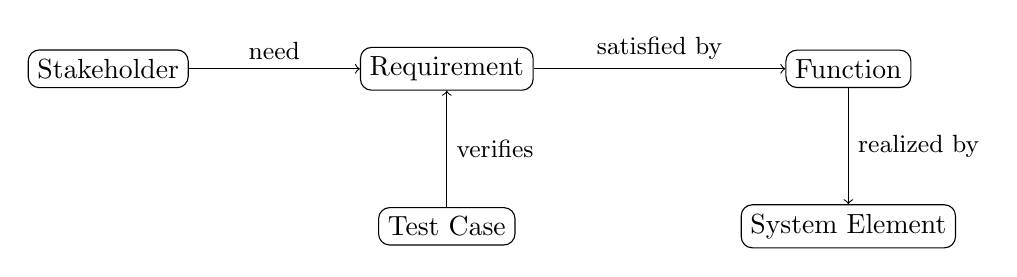
\begin{tikzpicture}[node distance=1.6cm]
\node (stakeholder) [draw, rounded corners] {Stakeholder};
\node (req) [draw, rounded corners, right of=stakeholder, xshift=2.7cm] {Requirement};
\node (func) [draw, rounded corners, right of=req, xshift=3.5cm] {Function};
\node (arch) [draw, rounded corners, below of=func, yshift=-0.4cm] {System Element};
\node (test) [draw, rounded corners, left of=arch, xshift=-3.5cm] {Test Case};
\draw[->] (stakeholder) -- node[above] {\small need} (req);
\draw[->] (req) -- node[above] {\small satisfied by} (func);
\draw[->] (func) -- node[right] {\small realized by} (arch);
\draw[->] (test) -- node[right] {\small verifies} (req);
\end{tikzpicture}

}
  \caption{From document to model relationship: a stakeholder need leads to a requirement, which is satisfied by a function and realized by a system element; a test case verifies the requirement.}
  \label{fig:kap02-dokumente-modellbeziehungen}
\end{figure}

This simple picture already shows the core of MBSE. The point is not to produce many diagrams. The point is to connect system information so that questions become answerable.

\subsection{Traceability}
Traceability lets you follow the links from a requirement to the design and the tests that verify it. You can jump from one piece of information to related ones. From a requirement, you reach functions, components, and tests. From a component, you can see which requirements it satisfies. From a test, you can see which requirement it checks.

For the indoor robot, traceability is especially useful. If the safety requirement is tightened, the team wants to know:

\begin{itemize}
    \item Which functions are affected?
    \item Which sensors and software components are involved?
    \item Which interfaces need to change?
    \item Which tests need to be extended?
    \item What risks arise for cost, schedule, and battery life?
\end{itemize}

Without a model, the team must dig these connections out of documents by hand. With a well-maintained model, at least part of this becomes directly visible.

\section{MBSE in the Robot Project}
For our textbook project, we model the autonomous indoor robot step by step. The model grows together with our understanding. At the start, it does not need to be complete. It should make the most important relationships visible.

\subsection{First Model Structure}
A simple starting structure for the model could look like this:

\begin{itemize}
    \item package \enquote{Stakeholders and Context}
    \item package \enquote{Requirements}
    \item package \enquote{Functions}
    \item package \enquote{System Structure}
    \item package \enquote{Interfaces}
    \item package \enquote{Behavior}
    \item package \enquote{ROS2 Architecture}
    \item package \enquote{Tests and Verification}
\end{itemize}

At this point, a package is just an organizing area. It helps keep the model tidy. Later, we will see how such packages can be set up concretely as SysML v2 files and namespaces.

\subsection{Example Chain: Obstacle Detection}
Consider a typical model chain:

\begin{enumerate}
    \item Stakeholder need: people in the building must not be endangered.
    \item Requirement: the robot must detect obstacles in its path and stop in time.
    \item Function: detect obstacle.
    \item Function: limit movement safely.
    \item System element: lidar sensor.
    \item System element: safety logic.
    \item ROS2 element: topic for sensor data.
    \item ROS2 element: node for obstacle evaluation.
    \item Test case: check stopping behavior for an obstacle at a defined distance.
\end{enumerate}

This chain shows how MBSE bridges from a human need all the way to a technical test. This bridge is exactly what makes MBSE valuable in complex projects. Figure~\ref{fig:kap02-modellkette-traceability} shows this model chain with color coding, from the requirement (blue) through functions and system elements (green) to ROS2 elements (orange) and the test case (gray).

\begin{figure}[H]
  \centering
  \adjustbox{max width=\linewidth,max totalheight=0.6\textheight}{% =====================================================================
% Figure: Model chain: from requirement to test case (obstacle detection)
% Belongs with chapter 2, section "Example Chain: Obstacle Detection"
% (subsection of "MBSE in the Robot Project")
%
% Used in the book, e.g. in chapters_en/02_mbse.tex:
%
%   \begin{figure}[H]
%     \centering
%     % =====================================================================
% Figure: Model chain: from requirement to test case (obstacle detection)
% Belongs with chapter 2, section "Example Chain: Obstacle Detection"
% (subsection of "MBSE in the Robot Project")
%
% Used in the book, e.g. in chapters_en/02_mbse.tex:
%
%   \begin{figure}[H]
%     \centering
%     \input{figures_en/fig_kap02_modellkette_traceability}
%     \caption{Color-coded model chain from a stakeholder need, through
%       a requirement, functions, and system elements, to a ROS2 node
%       and a test case.}
%     \label{fig:kap02-modellkette-traceability}
%   \end{figure}
%
% Required packages (already loaded in main_en.tex): tikz
% Required TikZ libraries: positioning, arrows.meta, shadows, calc
% =====================================================================

\input{figures_en/fig_kap02_modellkette_traceability.tikz}

%     \caption{Color-coded model chain from a stakeholder need, through
%       a requirement, functions, and system elements, to a ROS2 node
%       and a test case.}
%     \label{fig:kap02-modellkette-traceability}
%   \end{figure}
%
% Required packages (already loaded in main_en.tex): tikz
% Required TikZ libraries: positioning, arrows.meta, shadows, calc
% =====================================================================

\begin{tikzpicture}[
    every node/.style={font=\small},
    ext/.style={
        rectangle, rounded corners=1.5pt, draw=black!50, thick, dashed,
        minimum width=24mm, minimum height=13mm,
        align=center, fill=white, drop shadow, font=\scriptsize
    },
    req/.style={
        rectangle, rounded corners=1.5pt, draw=black!70, thick,
        minimum width=24mm, minimum height=13mm,
        align=center, fill=blue!12, drop shadow, font=\scriptsize
    },
    part/.style={
        rectangle, rounded corners=1.5pt, draw=green!40!black, thick,
        minimum width=24mm, minimum height=13mm,
        align=center, fill=green!15, drop shadow, font=\scriptsize
    },
    tool/.style={
        rectangle, rounded corners=1.5pt, draw=orange!60!black, thick,
        minimum width=24mm, minimum height=13mm,
        align=center, fill=orange!15, drop shadow, font=\scriptsize
    },
    test/.style={
        rectangle, rounded corners=1.5pt, draw=black!50, thick,
        minimum width=24mm, minimum height=13mm,
        align=center, fill=black!6, drop shadow, font=\scriptsize
    },
    flow/.style={-{Stealth[length=2.2mm]}, thick, black!60}
]

% --- Row 1: stakeholder need to system element lidar sensor ---
\node[ext]  (need) at (1.2,3.5)  {Stakeholder\\Need};
\node[req]  (req)  at (4.0,3.5)  {Requirement};
\node[part] (f1)   at (6.8,3.5)  {Function:\\Detect\\Obstacle};
\node[part] (f2)   at (9.6,3.5)  {Function:\\Limit Movement\\Safely};
\node[part] (lidar)at (12.4,3.5) {System Element:\\Lidar Sensor};

\draw[flow] (need) -- (req);
\draw[flow] (req)  -- (f1);
\draw[flow] (f1)   -- (f2);
\draw[flow] (f2)   -- (lidar);

% --- Row 2: system element safety logic to test case ---
\node[part] (safety) at (12.4,0) {System Element:\\Safety Logic};
\node[tool] (topic)  at (9.6,0)  {ROS2 Topic};
\node[tool] (rosnode)   at (6.8,0)  {ROS2 Node};
\node[test] (tc)     at (4.0,0)  {Test Case};

\draw[flow] (lidar.south)  -- (safety.north);
\draw[flow] (safety) -- (topic);
\draw[flow] (topic)  -- (rosnode);
\draw[flow] (rosnode)   -- (tc);

% --- Legend ---
\node[req, minimum width=6mm, minimum height=4mm, font=\tiny] (leg1) at (1.2,-2.2) {};
\node[right=1mm of leg1, font=\tiny, align=left] (lab1){Requirement};
\node[part, minimum width=6mm, minimum height=4mm, font=\tiny, right=6mm of lab1] (leg2) {};
\node[right=1mm of leg2, font=\tiny, align=left] (lab2){Function / System Element};
\node[tool, minimum width=6mm, minimum height=4mm, font=\tiny, right=6mm of lab2] (leg3) {};
\node[right=1mm of leg3, font=\tiny, align=left] (lab3){ROS2 Element};
\node[test, minimum width=6mm, minimum height=4mm, font=\tiny, right=6mm of lab3] (leg4) {};
\node[right=1mm of leg4, font=\tiny, align=left] (lab4){Test Case};

\end{tikzpicture}

}
  \caption{Color-coded model chain from a stakeholder need, through a requirement, functions, and system elements, to a ROS2 node and a test case.}
  \label{fig:kap02-modellkette-traceability}
\end{figure}

\subsection{Example Chain: Battery Management}
A second chain concerns the battery:

\begin{enumerate}
    \item Stakeholder need: the robot must not stop in the middle of a corridor.
    \item Requirement: the robot must return to the charging station on its own when its battery is low.
    \item Function: monitor battery level.
    \item Function: plan return to charging station.
    \item System element: battery.
    \item System element: battery management.
    \item System element: navigation.
    \item ROS2 element: battery state message.
    \item Test case: check the return to the charging station once a threshold is crossed.
\end{enumerate}

Here, too, you can see that the requirement does not touch just one single component. It connects power supply, software, navigation, charging infrastructure, and testing.

\section{The Benefit of MBSE}
MBSE is not an end in itself. The benefit only appears when the model answers real project questions. The main advantages are traceability, consistency, communication, change analysis, and better preparation for implementation.

\subsection{Traceability}
Traceability means that decisions and connections stay recognizable. If someone asks why the robot has a lidar sensor, the model should not just show \enquote{because we decided so} -- it should show the connection to requirements and functions.

\subsection{Consistency}
A model can help avoid contradictions. If a system element gets renamed, it appears with the same name in every view. If a requirement has no test case, that can be flagged. If a function is not assigned to any component, this becomes an open question.

\subsection{Communication}
Diagrams and structured models help teams talk about the same system. This matters especially in a robot project, because different disciplines are involved. A shared model structure can reduce misunderstandings.

\subsection{Change Analysis}
Changes are normal. MBSE helps you understand the consequences of a change. If the maximum speed increases, that does not just affect the motors. It also affects braking distance, obstacle detection, safety logic, battery life, tests, and possibly approval questions.

\subsection{A Bridge to Implementation}
In this textbook, one point matters especially: the model should later fit the ROS2 architecture. We do not want to model the system and then reinvent everything afterward. We want to understand how requirements, functions, and system elements can map onto nodes, topics, services, parameters, and tests.

\begin{praxisbox}
A SysML function \enquote{detect person} can later map onto a ROS2 node \texttt{object\_detector\_node}. The interface of this function can lead to topics for camera images and detected objects. This creates a traceable connection between the system model and the software structure.
\end{praxisbox}

\section{Limits and Misunderstandings}
MBSE helps manage complexity. But it does not automatically solve every problem. A model can be wrong, outdated, or needlessly complicated. Then it creates more effort than benefit.

\subsection{Misunderstanding 1: MBSE Means Modeling Everything}
A good model does not contain every detail. It contains the details that matter for understanding, decisions, interfaces, risks, and evidence. A model that maps every tiny software parameter can become unmanageable. A model that contains only three pretty pictures is too shallow.

\subsection{Misunderstanding 2: The Model Replaces Communication}
A model supports communication, but it does not replace it. People must still ask questions, make decisions, and clarify assumptions. The model documents and connects the results.

\subsection{Misunderstanding 3: The Tool Does the Engineering}
A SysML v2 tool can check relationships, generate views, and support consistency checks. It does not decide which requirements make sense or which architecture is good. That remains engineering work.

\subsection{Misunderstanding 4: MBSE Is Only for Large Corporations}
MBSE is often associated with large aerospace, automotive, or space projects. The core idea, though, is useful for small projects too. A learning project benefits especially, because it makes relationships visible. You only need to choose the right scope.

\begin{hinweisbox}
For this textbook, the rule is: we model enough to make the connections between SysML v2, MBSE, and ROS2 understandable. We do not model every conceivable detail of the robot.
\end{hinweisbox}

\section{A Pragmatic Start with MBSE}
Beginners should not start MBSE with the goal of building a perfect model right away. A step-by-step start works better.

\subsection{Step 1: Describe Purpose and Context}
First, describe what the system is built for and in which environment it operates. For the robot: indoor spaces, a defined area of a building, people nearby, a charging station, a user interface, and a possible network connection.

\subsection{Step 2: Collect Requirements}
Next, collect the important requirements. They do not need to be perfect at the start. What matters is making them visible, then improving them later. Good requirements are understandable, unambiguous, and testable.

\subsection{Step 3: Derive Functions}
Functions get derived from requirements. If the robot must return to the charging station automatically, it needs functions such as \enquote{monitor battery level,} \enquote{locate charging station,} and \enquote{plan return.}

\subsection{Step 4: Design the Structure}
Next, decide which system elements realize the functions. This is where the first system parts appear (\texttt{part def}, explained in more detail in chapter 3), along with subsystems or components. For the robot, these are, for example, sensors, navigation, power supply, and the user interface.

\subsection{Step 5: Describe Interfaces}
Interfaces should be described early. Who provides which data? Who needs which information? What signals, messages, or energy flows exist?

\subsection{Step 6: Assign Tests}
Tests or other evidence get assigned to the important requirements. This keeps it clear how the team plans to check later whether the system works.

\section{Quality Traits of a Good Model}
An MBSE model is not automatically good just because it is big. Good models share a few practical traits.

\subsection{Clarity}
A new team member should be able to find their way around the model. Names should be self-explanatory. Diagrams should not be overloaded. The structure should be easy to follow.

\subsection{Consistency}
Terms should be used consistently. If a component is called \enquote{Battery Monitor} in one place, \enquote{battery module} in another, and \enquote{Power Node} in a third, misunderstandings follow. For a German textbook, German terms can make sense in the system model, while later ROS2 package names stay technically English.

\subsection{Appropriate Depth}
The model should be neither too coarse nor too detailed. A good question to ask is: \enquote{Does this detail help with a decision, an interface, an implementation, or a check?} If not, it may not belong in a beginner's model.

\subsection{Maintainability}
A model must be maintainable. If every small change requires a lot of manual rework, the model quickly falls out of date. A simple, clear model structure is therefore important.

\subsection{Verifiability}
Important requirements should be connected to evidence. Not every requirement needs a fully worked-out test right away, but it should be clear how its fulfilment will be checked later.

\section{Views and Roles in the Model}
A system model holds a lot of information. Even so, not everyone needs to see all of it all the time. This is why MBSE works with views. A view shows a specific slice of the model for a specific question or role.

This is similar to a map of a building. An architect looks at floor plans, an electrician looks at power lines, the fire department looks at escape routes, and a visitor looks at the site plan. All these views describe the same building, but they show different information.

\subsection{The Project Management View}
Project management cares mainly about progress, risks, open decisions, and the effects of changes. In the MBSE model, this could mean answering questions such as:

\begin{itemize}
    \item Which requirements are still unresolved?
    \item Which requirements have no evidence yet?
    \item Which subsystems are most affected by changes?
    \item Which interfaces are not yet described?
    \item Which risks affect safety, cost, or schedule?
\end{itemize}

For project management, the model is therefore not a technical picture book, but a steering tool. It shows where uncertainty lies.

\subsection{The System Architecture View}
The system architecture view looks at the major building blocks and their relationships. For the robot, this means, for example, the split into sensors, localization, navigation, propulsion, power supply, operation, and safety functions. This view answers questions such as:

\begin{itemize}
    \item Which main systems exist?
    \item Which data and signals flow between them?
    \item Where are the critical interfaces?
    \item Which functions belong to which subsystem?
    \item Which components are responsible for safety-relevant behavior?
\end{itemize}

\subsection{The Software Development View}
Software development cares about data flows, states, sequences, responsibilities, and technical interfaces. In our project, this view becomes especially important later, because we want to connect SysML with ROS2.

A software developer wants to know:

\begin{itemize}
    \item Which ROS2 nodes are needed?
    \item Which topics carry sensor data, status information, or control commands?
    \item Which services or actions fit tasks and navigation?
    \item Which parameters must be configurable?
    \item Which fault states must the software detect?
\end{itemize}

The MBSE model does not yet deliver finished code for this. It does deliver a structured foundation, so the software architecture does not emerge by accident.

\subsection{The Test Team View}
The test team wants to know what must be checked and how tests connect to requirements. One especially important question is whether every central requirement has evidence attached to it.

For the indoor robot, test views could show:

\begin{itemize}
    \item requirements for obstacle detection and matching test scenarios
    \item requirements for battery life and measurement procedures
    \item robot states and tests for state transitions
    \item interfaces between ROS2 nodes and integration tests
    \item fault situations and the expected safe responses
\end{itemize}

This view stops tests from being invented only at the end. Good tests grow alongside the team's understanding of the system.

Figure~\ref{fig:kap02-sichten-auf-modell} summarizes the four views described above once more: all of them access the same model, but look at it from different angles.

\begin{figure}[H]
  \centering
  \adjustbox{max width=\linewidth,max totalheight=0.6\textheight}{% =====================================================================
% Figure: Views onto a shared model
% Belongs with chapter 2, section "Views and Roles in the Model"
%
% Used in the book, e.g. in chapters_en/02_mbse.tex:
%
%   \begin{figure}[H]
%     \centering
%     % =====================================================================
% Figure: Views onto a shared model
% Belongs with chapter 2, section "Views and Roles in the Model"
%
% Used in the book, e.g. in chapters_en/02_mbse.tex:
%
%   \begin{figure}[H]
%     \centering
%     \input{figures_en/fig_kap02_sichten_auf_modell}
%     \caption{Four roles look at the same MBSE model of the robot
%       from different angles.}
%     \label{fig:kap02-sichten-auf-modell}
%   \end{figure}
%
% Required packages (already loaded in main_en.tex): tikz
% Required TikZ libraries: positioning, arrows.meta, shadows, calc
% =====================================================================

\input{figures_en/fig_kap02_sichten_auf_modell.tikz}

%     \caption{Four roles look at the same MBSE model of the robot
%       from different angles.}
%     \label{fig:kap02-sichten-auf-modell}
%   \end{figure}
%
% Required packages (already loaded in main_en.tex): tikz
% Required TikZ libraries: positioning, arrows.meta, shadows, calc
% =====================================================================

\begin{tikzpicture}[
    every node/.style={font=\small},
    center/.style={
        rectangle, rounded corners=1.5pt, draw=green!40!black, thick,
        minimum width=34mm, minimum height=14mm,
        align=center, fill=green!15, drop shadow
    },
    role/.style={
        rectangle, rounded corners=1.5pt, draw=black!50, thick, dashed,
        minimum width=32mm, minimum height=13mm,
        align=center, fill=white, drop shadow
    },
    conn/.style={black!45, dashed, thick}
]

% --- Center ---
\node[center] (modell) at (6,3) {MBSE Model\\of the Robot};

% --- Four views/roles ---
\node[role] (pl)  at (6,5.65)  {Project Management\\(progress, risks)};
\node[role] (arch) at (11,3) {System Architecture\\(building blocks, interfaces)};
\node[role] (sw)  at (5.99,0.35)  {Software Development\\(nodes, topics)};
\node[role] (test) at (1,3)  {Test Team\\(requirements $\leftrightarrow$ tests)};

\draw[conn] (modell) -- (pl);
\draw[conn] (modell) -- (arch);
\draw[conn] (modell) -- (sw);
\draw[conn] (modell) -- (test);

% --- Legend ---
\node[center, minimum width=6mm, minimum height=4mm, font=\tiny] (leg1) at (2.74,-1.34) {};
\node[right=1mm of leg1, font=\tiny, align=left] (lab1){shared model};
\node[role, minimum width=6mm, minimum height=4mm, font=\tiny, right=6mm of lab1] (leg2) {};
\node[right=1mm of leg2, font=\tiny, align=left] (lab2){view/role on the model};

\end{tikzpicture}

}
  \caption{Four roles look at the same MBSE model of the robot from different angles.}
  \label{fig:kap02-sichten-auf-modell}
\end{figure}

\section{From the MBSE Model to the ROS2 Architecture}
One central goal of this textbook is to connect SysML v2, MBSE, and ROS2. It is therefore important to understand early on how a system model can lead to a later software structure.

This transition does not happen automatically. A SysML system element does not turn into a ROS2 node by magic. But the model can systematically prepare which software units make sense and how they communicate with each other.

\subsection{Functions as a Starting Point}
Functions come first. Functions describe what the system must do. For the robot, these are, for example, \enquote{sense the environment,} \enquote{determine position,} \enquote{plan a route,} \enquote{avoid obstacles,} \enquote{detect people,} and \enquote{monitor battery level.}

These functions can later map onto software building blocks. Not every function automatically becomes its own node. Sometimes several functions get grouped into one node. Sometimes one function gets split across several nodes. Modeling helps the team make this decision deliberately.

\subsection{Data Flows as Preparation for Topics}
ROS2 systems often communicate over topics. A topic carries messages from one sender to one or more receivers. In the MBSE model, data flows can be prepared before concrete topic names get decided.

Examples:

\begin{itemize}
    \item The camera sends image data to people detection.
    \item The lidar sends distance data to obstacle evaluation.
    \item Localization sends the current pose to navigation.
    \item Navigation sends speed targets to drive control.
    \item Battery management sends charge level to mission planning.
\end{itemize}

Later, these can become ROS2 topics such as \texttt{/camera/image}, \texttt{/scan}, \texttt{/robot\_pose}, \texttt{/cmd\_vel}, or \texttt{/battery\_state}. The exact names are technical decisions. But the underlying communication structure can already become visible in the model.

\subsection{States as a Basis for Control Logic}
An autonomous robot has operating states. Examples are \enquote{ready,} \enquote{task active,} \enquote{navigating,} \enquote{obstacle detected,} \enquote{returning,} \enquote{charging,} and \enquote{fault.} These states can be modeled in SysML and help later during software development.

Without a state model, control logic often ends up scattered through the code. After a while, no one knows exactly when the robot may drive, when it must stop, or how it recovers from a fault state. A state model creates a shared foundation.

\subsection{Tests as the Link Between Model and Code}
Tests form an important bridge between the model and the implementation. If a requirement in the model is linked to a test case, the later code can be checked specifically against this expectation.

Example:

\begin{enumerate}
    \item Requirement: the robot must return to the charging station when its battery is low.
    \item Model function: trigger return to the charging station.
    \item ROS2 node: \texttt{battery\_monitor\_node} reports a low charge level.
    \item ROS2 node: \texttt{navigation\_node} receives the \enquote{charging station} target.
    \item Test: simulated battery level drops below the threshold, and a return target is then set.
\end{enumerate}

In this way, a functional expectation becomes a testable technical implementation.

\section{Typical Mistakes When Starting with MBSE}
MBSE, too, can be applied the wrong way. Especially at the start, a few warning signs help.

\subsection{Mistake 1: Diagrams Without Model Content}
The team draws nice diagrams, but the elements are not named cleanly, not reused, and not linked. This produces only a prettier form of document-centric development.

\subsection{Mistake 2: Too Many Details Too Early}
Beginners sometimes try to model every cable, every software class, and every parameter right away. This makes the model large before the basic structure is understood. It works better to start with requirements, main functions, main systems, and critical interfaces.

\subsection{Mistake 3: No Model Maintenance}
A model is only useful if it is maintained. If architecture decisions change in the code but never flow back into the model, the model loses its value. The project must therefore make clear which parts of the model are maintained as a binding source of truth.

\subsection{Mistake 4: Unclear Modeling Rules}
If every team member models differently, disorder follows. Even simple rules help: consistent names, a clear package structure, defined relationship types, and limited diagram sizes.

\subsection{Mistake 5: Model and Implementation Become Separate Worlds}
The model must not run alongside development like a box-ticking exercise. It must answer questions that really come up in the project. In this textbook, the connection to the ROS2 architecture therefore matters: the model should not just explain, it should prepare the implementation.

\section{Summary}
\gls{mbse} carries the ideas of systems engineering into a model-based way of working. Instead of spreading project knowledge across many loose documents, key information gets structured and linked within a system model. The model holds requirements, functions, structure, interfaces, behavior, tests, assumptions, and decisions.

The most important point is not drawing diagrams, but building relationships. A requirement does not stand alone. It connects to stakeholders, functions, system elements, interfaces, and tests. This traceability is exactly what makes MBSE valuable.

For the autonomous indoor robot, this means: we can think from a user's need, through requirements and functions, all the way to the later ROS2 architecture. The model becomes a bridge between understanding the problem, SysML v2 modeling in the Syside Editor, and technical implementation.

\section{Review Questions}
\begin{enumerate}
    \item What does Model-Based Systems Engineering mean?
    \item How does a model differ from a simple diagram image?
    \item Why does document-centric development become problematic in more complex projects?
    \item What kinds of information can an MBSE model contain?
    \item What is traceability?
    \item Why does traceability matter for requirements and tests?
    \item Name three typical model relationships in the robot project.
    \item Why doesn't MBSE replace the source code?
    \item Why doesn't MBSE replace communication within the team?
    \item What advantages does MBSE offer when things change?
    \item What would be an example of modeling that is too detailed?
    \item Which packages would you create for a first model of the indoor robot?
\end{enumerate}

\section{Exercises}
\begin{uebungbox}
\textbf{Exercise 1: Spot Document Chaos}\\
Make a list of five documents or information sources that could arise in a typical robot project. For each source, describe the risk that appears if it is not kept up to date.
\end{uebungbox}

\begin{uebungbox}
\textbf{Exercise 2: Build a Model Chain}\\
Build a simple chain from stakeholder need, requirement, function, system element, and test case for the automatic return to the charging station.
\end{uebungbox}

\begin{uebungbox}
\textbf{Exercise 3: Link Requirements}\\
Choose three requirements for the indoor robot. For each requirement, assign at least one function, one possible system element, and one test case.
\end{uebungbox}

\begin{uebungbox}
\textbf{Exercise 4: Limit Model Scope}\\
Note down ten possible pieces of information about the robot. For each one, decide whether it belongs in a beginner's MBSE model or can stay outside it for now. Give a short reason for each decision.
\end{uebungbox}

\begin{uebungbox}
\textbf{Exercise 5: Change Analysis}\\
Suppose the robot's maximum speed increases from 0.8 m/s to 1.2 m/s. Describe which requirements, functions, components, interfaces, and tests this could affect.
\end{uebungbox}

\section{Further Reading}
For getting started with MBSE, practice-oriented introductions to SysML are especially helpful, because they treat modeling not abstractly but through requirements, architecture, and behavior. Particularly recommended are the works on SysML already cited in this project, for example Delligatti \cite{delligatti2014} and Friedenthal, Moore, and Steiner \cite{friedenthal2014}.

Beyond that, further reading on systems engineering, requirements management, verification and validation, and model-based development of cyber-physical systems pays off. For later technical implementation, the ROS2 documentation \cite{ros2docs} is also important, because it shows how software architectures with nodes, topics, services, actions, and parameters are built in practice.

\chapter{SysML Fundamentals}

\begin{lernziele}
After this chapter, you know the basic idea of \gls{sysml} v2, the key modeling concepts, and their role in an MBSE project. You can explain why a SysML diagram is only one view of a model, which concepts matter most for getting started, and how these concepts work together in the autonomous indoor robot.
\end{lernziele}

\section{Introduction}
In the first two chapters, we explained why Systems Engineering and MBSE are useful. Now we need a language that lets us describe requirements, structure, behavior, interfaces, and tests precisely. In this book, that language is \gls{sysml} v2.

\gls{sysml} stands for Systems Modeling Language. Engineers designed it to model technical systems. SysML v2 is a complete redesign of SysML v1, with a precise textual notation and clear, modern semantics. It focuses more strongly than UML on systems that combine hardware, software, people, processes, data, and physical relationships. That fits our autonomous indoor robot well: it consists not only of software, but also of sensors, a drive system, a battery, a housing, a charging station, a user interface, and a real physical environment.

For beginners, one point matters most: SysML is not a drawing program. SysML is a modeling language. A diagram is only a visible representation of model elements. The real value lies in the model itself: requirements link to system parts, system parts have interfaces, behavior describes sequences of steps, and tests verify requirements.

\section{Why a Modeling Language?}
Without a shared language, projects quickly run into misunderstandings. One team member draws boxes for functions, another for software modules, a third for hardware components. All the diagrams look similar, but they mean different things. SysML helps clarify such meanings.

SysML v2 provides predefined concepts:

\begin{itemize}
    \item \texttt{requirement} for requirements
    \item \texttt{part def} and \texttt{part} for system elements and their instances
    \item \texttt{port} and \texttt{connection} for interfaces
    \item \texttt{action def} and \texttt{action} for sequences of steps
    \item \texttt{state def} and \texttt{state} for states
    \item \texttt{calc def} and \texttt{constraint} for mathematical relationships
    \item \texttt{satisfy}, \texttt{verify}, \texttt{derive} for traceability
\end{itemize}

With these concepts, a team can talk about the same system without re-explaining every symbol.

\begin{praxisbox}
Suppose the model contains a \texttt{part def PerceptionSystem}. In a structure view, it can appear as part of the robot. In a connection view, it can link to the camera and the lidar. Through a \texttt{satisfy} relationship, it can fulfill requirements for obstacle detection. It is the same model content, just seen from different angles.
\end{praxisbox}

\section{Key Concepts in SysML v2}
SysML v2 no longer has fixed diagram types like SysML v1. Instead, it offers views (\emph{views}) and viewpoints (\emph{viewpoints}) onto one shared model. A viewpoint defines the kind of question a view should answer, for example structure or behavior; the view itself is the concrete representation generated from it. To get started, we focus on the concepts that bring the most value to the robot project. Figure~\ref{fig:kap03-sysml-kernkonzepte} gives an overview of the seven most important concepts before we introduce them one by one.

\begin{figure}[H]
  \centering
  \adjustbox{max width=\linewidth,max totalheight=0.6\textheight}{% =====================================================================
% Figure: Overview of the SysML v2 core concepts
% Belongs to chapter 3, section "Key Concepts in SysML v2"
%
% Used in the book, e.g. in chapters_en/03_sysml_grundlagen.tex:
%
%   \begin{figure}[H]
%     \centering
%     % =====================================================================
% Figure: Overview of the SysML v2 core concepts
% Belongs to chapter 3, section "Key Concepts in SysML v2"
%
% Used in the book, e.g. in chapters_en/03_sysml_grundlagen.tex:
%
%   \begin{figure}[H]
%     \centering
%     \input{figures_en/fig_kap03_sysml_kernkonzepte}
%     \caption{The seven SysML v2 concepts that matter most for this book,
%       built around the shared model.}
%     \label{fig:kap03-sysml-kernkonzepte}
%   \end{figure}
%
% Required packages (already loaded in main_en.tex): tikz
% Required TikZ libraries: positioning, arrows.meta, shadows, calc
% =====================================================================

\input{figures_en/fig_kap03_sysml_kernkonzepte.tikz}

%     \caption{The seven SysML v2 concepts that matter most for this book,
%       built around the shared model.}
%     \label{fig:kap03-sysml-kernkonzepte}
%   \end{figure}
%
% Required packages (already loaded in main_en.tex): tikz
% Required TikZ libraries: positioning, arrows.meta, shadows, calc
% =====================================================================

\begin{tikzpicture}[
    every node/.style={font=\small},
    hub/.style={
        rectangle, rounded corners=1.5pt, draw=black!70, thick,
        minimum width=34mm, minimum height=14mm,
        align=center, fill=black!8, drop shadow
    },
    req/.style={
        rectangle, rounded corners=1.5pt, draw=black!70, thick,
        minimum width=30mm, minimum height=13mm,
        align=center, fill=blue!12, drop shadow
    },
    part/.style={
        rectangle, rounded corners=1.5pt, draw=green!40!black, thick,
        minimum width=30mm, minimum height=13mm,
        align=center, fill=green!15, drop shadow
    },
    test/.style={
        rectangle, rounded corners=1.5pt, draw=black!50, thick,
        minimum width=30mm, minimum height=13mm,
        align=center, fill=black!6, drop shadow
    },
    conn/.style={-{Stealth[length=2mm]}, thick, black!55}
]

% --- Center ---
\node[hub] (modell) at (5,4) {SysML v2\\Model};

% --- Seven core concepts in a circle ---
\node[req]  (anf)   at (5,8.3)     {Requirements\\ \texttt{requirement}};
\node[part] (strukt)at (8.36,6.68) {Structure\\ \texttt{part def}, \texttt{part}};
\node[part] (verb)  at (9.19,3.05) {Connections\\ \texttt{port}, \texttt{connection}};
\node[part] (verh)  at (6.86,0.12) {Behavior\\ \texttt{action def}, \texttt{action}};
\node[part] (zust)  at (3.14,0.12) {States\\ \texttt{state def}, \texttt{state}};
\node[part] (param) at (0.81,3.05) {Parametrics\\ \texttt{calc def}, \texttt{constraint}};
\node[test] (trace) at (1.64,6.68) {Traceability\\ \texttt{satisfy}, \texttt{verify}, \texttt{derive}};

\draw[conn] (modell) -- (anf);
\draw[conn] (modell) -- (strukt);
\draw[conn] (modell) -- (verb);
\draw[conn] (modell) -- (verh);
\draw[conn] (modell) -- (zust);
\draw[conn] (modell) -- (param);
\draw[conn] (modell) -- (trace);

% --- Legend ---
\node[req, minimum width=7mm, minimum height=5mm, font=\scriptsize] (leg1) at (-0.35,-1.69) {};
\node[right=1mm of leg1, font=\scriptsize, align=left] (lab1){Requirement};
\node[part, minimum width=7mm, minimum height=5mm, font=\scriptsize, right=6mm of lab1] (leg2) {};
\node[right=1mm of leg2, font=\scriptsize, align=left] (lab2){Structure/Behavior/Connection};
\node[test, minimum width=7mm, minimum height=5mm, font=\scriptsize, right=6mm of lab2] (leg3) {};
\node[right=1mm of leg3, font=\scriptsize, align=left] (lab3){Traceability};

\end{tikzpicture}

}
  \caption{The seven SysML v2 concepts that matter most for this book, built around the shared model.}
  \label{fig:kap03-sysml-kernkonzepte}
\end{figure}

\subsection{Requirements (\texttt{requirement})}
Requirements describe what the system must do. In SysML v2, you define them as text with \texttt{requirement}. Relationships such as \texttt{satisfy}, \texttt{verify}, and \texttt{derive} connect requirements to system parts and test cases.

Typical questions:

\begin{itemize}
    \item What must the system do?
    \item Which requirements relate to each other?
    \item Which requirement was derived from which higher-level requirement?
    \item Which parts satisfy a requirement?
    \item Which tests check a requirement?
\end{itemize}

\subsection{Structure Modeling (\texttt{part def}, \texttt{part})}
In SysML v2, \texttt{part def} describes the type of a system element. \texttt{part} creates an instance of it. Together, they replace the block concept from SysML v1.

\begin{lstlisting}
package RobotStructure {
  part def Robot {
    part perceptionSystem : PerceptionSystem;
    part navigationSystem : NavigationSystem;
    part batterySystem    : BatterySystem;
    part motionControl    : MotionControl;
  }
  part def PerceptionSystem;
  part def NavigationSystem;
  part def BatterySystem;
  part def MotionControl;
}
\end{lstlisting}

This view answers the question: what are the system's main building blocks?

\subsection{Connection Modeling (\texttt{port}, \texttt{connection})}
A \texttt{port} describes how a system part connects to the outside. A \texttt{connection} links ports of different parts to each other. This makes visible how the parts of a system work together internally.

\begin{lstlisting}
part def PerceptionSystem {
  port sensorData : ~SensorDataPort;
  part camera  : Camera;
  part lidar   : Lidar;
  part detector : ObjectDetector;
}
\end{lstlisting}

\begin{hinweisbox}
The tilde character (\texttt{\textasciitilde}) marks a so-called conjugated port; we explain exactly what that means in chapter 9.
\end{hinweisbox}

\subsection{Behavior Modeling (\texttt{action def}, \texttt{action})}
Activities describe sequences of steps. They suit processes such as \enquote{Execute transport order}, \enquote{Return to charging station}, or \enquote{Handle obstacle}. In SysML v2, you model these sequences with \texttt{action def} and \texttt{action}.

\subsection{State Modeling (\texttt{state def}, \texttt{state})}
State models describe states and transitions. A robot has operating states such as \texttt{Idle}, \texttt{Navigating}, \texttt{AvoidingObstacle}, and \texttt{Charging}. In SysML v2, you define these with \texttt{state def}.

\subsection{Parametric Modeling (\texttt{calc def}, \texttt{constraint})}
Parametric models describe mathematical relationships. They help you check technical decisions early. In SysML v2, you express calculations with \texttt{calc def} and conditions with \texttt{constraint}.

You will learn behavior, states, and parametrics in detail starting in chapter 11. For the first steps in chapter 4, requirements and structure are enough.

\section{How Views Show the Model}
A SysML diagram is only one view of a model. This distinction is central. If you draw three boxes named \texttt{NavigationSystem} in a drawing program, they are three independent graphical objects. In a modeling tool such as the Syside Editor, \texttt{NavigationSystem} is a single model element that you can display in several views.

This has practical advantages:

\begin{itemize}
    \item Names stay consistent.
    \item You can evaluate relationships.
    \item Changes are easier to track.
    \item Different views show the same content.
    \item Traceability becomes possible.
\end{itemize}

\section{How the Concepts Work Together}
SysML v2 model elements should not stand alone. They complement each other.

For the indoor robot, a chain of models might look like this:

\begin{enumerate}
    \item The requirements model states: \enquote{The robot must detect obstacles.}
    \item You define \texttt{part def PerceptionSystem} as a system part.
    \item Ports and connections show how the camera and the lidar deliver data.
    \item An \texttt{action def} describes how the robot handles an obstacle while driving.
    \item A \texttt{state def} models that the robot switches to a stop or avoidance state when it detects danger.
    \item A test case connects to the requirement through \texttt{verify}.
\end{enumerate}

This builds a connected model instead of a loose collection of nice pictures. Figure~\ref{fig:kap03-struktur-verbindungssicht} shows, as an example, how the structure view and the connection view of \texttt{PerceptionSystem} work together: the overview shows the subsystems of \texttt{Robot}, and the detail view shows \texttt{PerceptionSystem} with its parts and the port \texttt{sensorData}.

\begin{figure}[H]
  \centering
  \adjustbox{max width=\linewidth,max totalheight=0.6\textheight}{% =====================================================================
% Figure: Structure and connection view of the PerceptionSystem
% Belongs to chapter 3, section "Model, Not Picture" /
% "How the Concepts Work Together"
%
% Used in the book, e.g. in chapters_en/03_sysml_grundlagen.tex:
%
%   \begin{figure}[H]
%     \centering
%     % =====================================================================
% Figure: Structure and connection view of the PerceptionSystem
% Belongs to chapter 3, section "Model, Not Picture" /
% "How the Concepts Work Together"
%
% Used in the book, e.g. in chapters_en/03_sysml_grundlagen.tex:
%
%   \begin{figure}[H]
%     \centering
%     \input{figures_en/fig_kap03_struktur_verbindungssicht}
%     \caption{Structure view of \texttt{Robot} with its subsystems, and
%       a detail view of \texttt{PerceptionSystem} with the port
%       \texttt{sensorData}.}
%     \label{fig:kap03-struktur-verbindungssicht}
%   \end{figure}
%
% Required packages (already loaded in main_en.tex): tikz
% Required TikZ libraries: positioning, arrows.meta, shadows, calc
% =====================================================================

\input{figures_en/fig_kap03_struktur_verbindungssicht.tikz}

%     \caption{Structure view of \texttt{Robot} with its subsystems, and
%       a detail view of \texttt{PerceptionSystem} with the port
%       \texttt{sensorData}.}
%     \label{fig:kap03-struktur-verbindungssicht}
%   \end{figure}
%
% Required packages (already loaded in main_en.tex): tikz
% Required TikZ libraries: positioning, arrows.meta, shadows, calc
% =====================================================================

\begin{tikzpicture}[
    every node/.style={font=\small},
    part/.style={
        rectangle, rounded corners=1.5pt, draw=green!40!black, thick,
        minimum width=26mm, minimum height=9mm,
        align=center, fill=green!15, drop shadow
    },
    container/.style={
        rectangle, rounded corners=2pt, draw=green!40!black, thick,
        align=center, fill=green!4, drop shadow
    },
    port/.style={rectangle, draw=black, fill=black!75, minimum width=2.2mm,
        minimum height=2.2mm, inner sep=0pt},
    portlbl/.style={font=\small},
    reflink/.style={-{Stealth[length=4mm]}, ultra thick, red!90, dashed}
]

% --- Outer structure view: Robot ---
\draw[container] (0.2,0.3) rectangle (6.2,5.3);
\node[font=\small\itshape, anchor=north west] at (0.3,5.2) {Robot};

\node[part] (perc) at (1.8,4.0) {perceptionSystem};
\node[part] (nav)  at (4.6,4.0) {navigationSystem};
\node[part] (batt) at (1.8,1.6) {batterySystem};
\node[part] (mot)  at (4.6,1.6) {motionControl};

% --- Detail box: PerceptionSystem with ports ---
\draw[container] (8.2,0.3) rectangle (13.6,5.3);
\node[font=\small\itshape, anchor=north west] at (8.3,5.2) {PerceptionSystem};

\node[part, minimum width=22mm] (camera)   at (10.0,4.1) {camera};
\node[part, minimum width=22mm] (lidar)    at (10.0,2.7) {lidar};
\node[part, minimum width=22mm] (detector) at (10.0,1.3) {detector};

\node[port] (sensport) at (13.6,2.7) {};
\node[portlbl, right=0.5mm of sensport, align=left]
    {\texttt{sensorData} \textcolor{orange!70!black}{$\sim$}};

\draw[black!55, thick] (detector.east) -- ++(1.6,0) |- (sensport.west);
\draw[black!55, thick] (camera.east)   -- ++(1.6,0) |- (sensport.west);
\draw[black!55, thick] (lidar.east)    -- (sensport.west);

% --- Reference between the overview and the detail box ---
\draw[reflink] (perc.east) to[bend left=15] node[above=1pt, font=\small, fill=white, inner sep=1pt, pos=0.67]
    {Detail view} (8.2,4.6);

% --- Legend ---
\node[part, minimum width=6mm, minimum height=4mm, font=\tiny] (leg1) at (0.5,-1.1) {};
\node[right=1mm of leg1, font=\small, align=left] (lab1) {\texttt{part} (instance of a \texttt{part def})};
\node[port, right=6mm of lab1] (leg2) {};
\node[right=1mm of leg2, font=\small, align=left] (lab2) {Port};
\node[right=6mm of lab2, font=\small, align=left] (lab3) {\textcolor{orange!70!black}{$\sim$} = conjugated port};

\end{tikzpicture}

}
  \caption{Structure view of \texttt{Robot} with its subsystems, and a detail view of \texttt{PerceptionSystem} with the port \texttt{sensorData}.}
  \label{fig:kap03-struktur-verbindungssicht}
\end{figure}

\section{SysML v1 and SysML v2 Compared}
Beginners often still run into SysML v1 in the literature. The most important terminology changes are:

\begin{center}
\adjustbox{max width=\linewidth}{%
\begin{tabular}{ll}
\toprule
\textbf{SysML v1} & \textbf{SysML v2} \\
\midrule
Block (block) & \texttt{part def} \\
Block Definition Diagram (BDD) & structure view (\texttt{part def}, \texttt{part}) \\
Internal Block Diagram (IBD) & connection view (\texttt{port}, \texttt{connection}) \\
Activity Diagram & \texttt{action def}, \texttt{action} \\
State Machine Diagram & \texttt{state def}, \texttt{state} \\
Parametric Diagram & \texttt{calc def}, \texttt{constraint} \\
\texttt{deriveRqt} & \texttt{derive} \\
\bottomrule
\end{tabular}%
}
\end{center}

This book uses SysML v2 throughout. Where it mentions old terms for compatibility reasons, it marks them explicitly.

\section{Typical Beginner Mistakes}
\subsection{Too Many Elements Too Soon}
Beginners often want to use every concept right away. That quickly leads to overload. Start with requirements, \texttt{part def}, and simple connections. Behavior and parametrics can follow later.

\subsection{Unclear Meaning of System Parts}
Sometimes functions, software modules, hardware parts, and roles get mixed together freely. That is not forbidden in principle, but it must happen on purpose. A \texttt{part def Camera} is a physical element. A \texttt{part def ObjectDetector} is more of a software or function component.

\subsection{Diagrams Without Text}
A diagram without a description is often hard to understand. Use documentation fields (\texttt{doc /* ... */}). Briefly state the purpose of each model element.

\subsection{No Reuse}
If you recreate the same element over and over, the model loses its value. Define types once with \texttt{part def}, and create instances with \texttt{part}.

\section{Summary}
SysML v2 is a modeling language for technical systems. It helps you describe requirements, structure, behavior, interfaces, and verification in one consistent way. For this book, \texttt{requirement}, \texttt{part def}, \texttt{port}, \texttt{connection}, \texttt{action def}, \texttt{state def}, and \texttt{calc def} matter most. What counts is not drawing individual diagrams, but building one connected model.

\section{Review Questions}
\begin{enumerate}
    \item What does SysML stand for?
    \item What distinguishes SysML v2 from SysML v1?
    \item What is the difference between a diagram and a model?
    \item Which questions does a requirements model answer?
    \item What is the difference between \texttt{part def} and \texttt{part}?
    \item What do \texttt{port} and \texttt{connection} do?
    \item When do you use \texttt{action def}?
    \item When do you use \texttt{state def}?
    \item Why should you reuse model elements?
    \item Name one typical beginner mistake in SysML.
\end{enumerate}

\section{Exercises}
\begin{uebungbox}
\textbf{Exercise 1: Match the Concept}\\
Match each question below to a SysML v2 concept: What must the system do? What parts does it consist of? What data flows between components? What states can the robot have? How does a transport order proceed?
\end{uebungbox}

\begin{uebungbox}
\textbf{Exercise 2: First Chain of Models}\\
Pick the function \enquote{Monitor battery level}. For it, describe a requirement, a \texttt{part def}, a port, a possible state, and a test case.
\end{uebungbox}

\begin{uebungbox}
\textbf{Exercise 3: v1 vs. v2}\\
For BDD, IBD, and Constraint Block, name the corresponding SysML v2 concept, and explain the difference in one sentence.
\end{uebungbox}

\section{Further Reading}
To get started with SysML v2, the official specification and the SysML v2 pilot project are essential \cite{sysmlv2pilot}. The Syside Editor has its own documentation and examples \cite{syside}. Older introductions such as Delligatti \cite{delligatti2014} and Friedenthal et al. \cite{friedenthal2014} describe SysML v1 and are useful only as background reading now.

\chapter{Setting Up Tools for SysML v2}

\begin{lernziele}
After this chapter, you can explain why this textbook uses a textual SysML v2 workflow. You can set up a simple project in VS Code with the Syside Editor and structure SysML v2 files. You can also write goal, scope and system boundary, requirements, part definitions, test cases, and ROS2 topic mappings in the SysML v2 text notation.
\end{lernziele}

\section{Introduction}
You can use SysML v2 graphically or textually. This textbook focuses on the textual notation. That fits modern development workflows well: models live in files, so you can version, compare, review, and maintain them together with code.

The Syside Editor for VS Code is a good free starting point. It supports SysML v2 files with syntax highlighting, autocomplete, formatting, outlining, and validation. For graphical views, you can also use Eclipse SysON. SysON is a web-based, open-source tool for SysML v2 models.

\begin{hinweisbox}
A tool does not solve a modeling task for you automatically. It helps you write, check, and display the model. The subject-matter decisions remain your job: Which elements exist? Which relationships matter? Which requirements must stay traceable?
\end{hinweisbox}

\section{Why Textual Modeling?}
Many beginners expect diagrams first when they hear "SysML". Diagrams remain important, but SysML v2 makes the model content accessible as precise text as well. That lets you treat a model more like source code.

Textual modeling has several advantages:

\begin{itemize}
    \item You can version models in Git.
    \item Changes show up as a text diff.
    \item You can show examples directly in the textbook.
    \item You can reuse model parts more easily.
    \item Validation and automation become simpler.
    \item ROS2 code and the SysML v2 model can live in the same project.
\end{itemize}

This does not make diagrams unimportant. Diagrams remain valuable views. The difference is: the model does not come only from drawing, but from precisely defined model elements.

\section{Recommended Toolchain}
For this textbook, we use a simple toolchain:

\begin{itemize}
    \item VS Code as the editor
    \item Syside Editor as the SysML v2 extension
    \item Git for version control
    \item optionally, Eclipse SysON for graphical views
    \item optionally, the SysML v2 pilot project as a reference for advanced experiments
\end{itemize}

This choice is deliberately pragmatic. It is free to use, fits textual modeling, and overwhelms beginners less than large industrial modeling environments. Figure~\ref{fig:kap04-werkzeugkette} shows this toolchain in context, including the parallel path to the ROS2 code.

\begin{figure}[H]
  \centering
  \adjustbox{max width=\linewidth,max totalheight=0.6\textheight}{% =====================================================================
% Figure: Toolchain for SysML v2 in the book
% Belongs to chapter 4, section "Recommended Toolchain"
%
% Used in the book, e.g. in chapters_en/04_sysml_v2_werkzeuge.tex:
%
%   \begin{figure}[H]
%     \centering
%     % =====================================================================
% Figure: Toolchain for SysML v2 in the book
% Belongs to chapter 4, section "Recommended Toolchain"
%
% Used in the book, e.g. in chapters_en/04_sysml_v2_werkzeuge.tex:
%
%   \begin{figure}[H]
%     \centering
%     \input{figures_en/fig_kap04_werkzeugkette}
%     \caption{Recommended toolchain: VS Code with the Syside Editor and
%       Git at its core, optionally extended with Eclipse SysON and the
%       SysML v2 pilot project; the ROS2 code runs alongside it.}
%     \label{fig:kap04-werkzeugkette}
%   \end{figure}
%
% Required packages (already loaded in main_en.tex): tikz
% Required TikZ libraries: positioning, arrows.meta, shadows, calc
% =====================================================================

\input{figures_en/fig_kap04_werkzeugkette.tikz}

%     \caption{Recommended toolchain: VS Code with the Syside Editor and
%       Git at its core, optionally extended with Eclipse SysON and the
%       SysML v2 pilot project; the ROS2 code runs alongside it.}
%     \label{fig:kap04-werkzeugkette}
%   \end{figure}
%
% Required packages (already loaded in main_en.tex): tikz
% Required TikZ libraries: positioning, arrows.meta, shadows, calc
% =====================================================================

\begin{tikzpicture}[
    every node/.style={font=\small},
    tool/.style={
        rectangle, rounded corners=1.5pt, draw=orange!60!black, thick,
        minimum width=27mm, minimum height=13mm,
        align=center, fill=orange!15, drop shadow
    },
    opt/.style={
        rectangle, rounded corners=1.5pt, draw=orange!60!black, thick, dashed,
        minimum width=27mm, minimum height=13mm,
        align=center, fill=orange!6, drop shadow
    },
    flow/.style={-{Stealth[length=2.2mm]}, thick, black!60},
    optflow/.style={{Stealth[length=2mm]}-{Stealth[length=2mm]}, thick, black!45, dashed},
    lbl/.style={font=\small, fill=white, inner sep=1pt}
]

% --- Main chain: editor -> version control -> optional tools ---
\node[tool, minimum height=62pt] (vscode) at (1.8,5.25)  {VS Code\\ + Syside Editor\\ (.sysml files)};
\node[tool, minimum height=41pt] (git)    at (1.8,2.55)  {Git\\ (version\\ control)};
\node[opt]  (syson)  at (1.8,0.48)  {Eclipse SysON\\ (graphical view)\\ \itshape optional};
\node[opt]  (pilot)  at (1.8,-1.56) {SysML v2\\pilot project\\ \itshape optional};

\draw[flow]    (vscode) -- node[lbl]{commit} (git);
\draw[optflow] (git)    -- node[lbl]{optional} (syson);
\draw[flow, dashed, black!45] (syson) -- node[lbl]{optional, reference} (pilot);

% --- Parallel path: ROS2 code ---
\node[tool] (code)  at (8.53,2.55) {\texttt{code/}\\ (ROS2 Python)};
\node[tool, minimum width=88pt, minimum height=39pt] (mapfile) at (8.53,5.18) {\texttt{model/}\\\texttt{07\_ros2\_}\\\texttt{mapping.sysml}};

\draw[flow] (code) -- node[lbl]{mapping} (mapfile);
\draw[flow] (mapfile.west) -- node[lbl]{part of the model} (vscode.east);

% --- Legend ---
\node[tool, minimum width=6mm, minimum height=4mm, font=\tiny] (leg1) at (5.09,-1.9) {};
\node[right=1mm of leg1, font=\tiny, align=left] (lab1){Tool/file (required)};
\node[opt, minimum width=6mm, minimum height=4mm, font=\tiny, right=6mm of lab1] (leg2) {};
\node[right=1mm of leg2, font=\tiny, align=left] (lab2){optional tool};

\end{tikzpicture}

}
  \caption{Recommended toolchain: VS Code with the Syside Editor and Git at its core, optionally extended with Eclipse SysON and the SysML v2 pilot project; the ROS2 code runs alongside it.}
  \label{fig:kap04-werkzeugkette}
\end{figure}

\section{Setting Up the Project}
For the textbook, we use a project named \texttt{AutonomousIndoorRobot}. The name is deliberately English, because later ROS2 packages, nodes, and topics also use English technical names. The explanatory text in the model can still be in your own language.

A simple project structure can look like this:

\begin{lstlisting}[style=plaintext]
AutonomousIndoorRobot/
  model/
    00_overview.sysml
    01_context.sysml
    02_requirements.sysml
    03_structure.sysml
    04_behavior.sysml
    05_interfaces.sysml
    06_tests.sysml
    07_ros2_mapping.sysml
  code/
    status_node.py
    battery_monitor_node.py
  docs/
    decisions.md
\end{lstlisting}

The files in the \texttt{model} folder hold the SysML v2 model. The \texttt{code} folder holds the later ROS2 examples. The \texttt{docs} folder can hold short architecture decisions. Figure~\ref{fig:kap04-projektstruktur} shows this project structure graphically and assigns a short keyword to each model file.

\begin{figure}[H]
  \centering
  \adjustbox{max width=\linewidth,max totalheight=0.6\textheight}{% =====================================================================
% Figure: Project structure of AutonomousIndoorRobot
% Belongs to chapter 4, section "Setting Up the Project" /
% "Recommended Model Structure"
%
% Used in the book, e.g. in chapters_en/04_sysml_v2_werkzeuge.tex:
%
%   \begin{figure}[H]
%     \centering
%     % =====================================================================
% Figure: Project structure of AutonomousIndoorRobot
% Belongs to chapter 4, section "Setting Up the Project" /
% "Recommended Model Structure"
%
% Used in the book, e.g. in chapters_en/04_sysml_v2_werkzeuge.tex:
%
%   \begin{figure}[H]
%     \centering
%     \input{figures_en/fig_kap04_projektstruktur}
%     \caption{Project structure \texttt{AutonomousIndoorRobot} with the
%       folders \texttt{model/}, \texttt{code/}, and \texttt{docs/}, and
%       its most important files.}
%     \label{fig:kap04-projektstruktur}
%   \end{figure}
%
% Required packages (already loaded in main_en.tex): tikz
% Required TikZ libraries: positioning, arrows.meta, shadows, calc
% =====================================================================

\input{figures_en/fig_kap04_projektstruktur.tikz}

%     \caption{Project structure \texttt{AutonomousIndoorRobot} with the
%       folders \texttt{model/}, \texttt{code/}, and \texttt{docs/}, and
%       its most important files.}
%     \label{fig:kap04-projektstruktur}
%   \end{figure}
%
% Required packages (already loaded in main_en.tex): tikz
% Required TikZ libraries: positioning, arrows.meta, shadows, calc
% =====================================================================

\begin{tikzpicture}[
    every node/.style={font=\small},
    root/.style={
        rectangle, rounded corners=1.5pt, draw=black!70, thick,
        minimum width=48mm, minimum height=10mm,
        align=center, fill=black!10, drop shadow, font=\small
    },
    folder/.style={
        rectangle, rounded corners=1.5pt, draw=orange!70!black, thick,
        minimum width=26mm, minimum height=9mm,
        align=center, fill=orange!28, drop shadow, font=\small
    },
    file/.style={
        rectangle, rounded corners=1.5pt, draw=orange!60!black, thick,
        minimum width=40mm, minimum height=10mm,
        align=center, fill=orange!12, drop shadow, font=\tiny
    },
    edg/.style={-{Stealth[length=2mm]}, thick, black!55},
    treeline/.style={thick, black!55}
]

% --- Root ---
\node[root] (root) at (7.9,10.6) {\texttt{AutonomousIndoorRobot/}};

% --- Folders ---
\node[folder] (model) at (3,9)   {\texttt{model/}};
\node[folder] (code)  at (8.0,9) {\texttt{code/}};
\node[folder] (docs)  at (12.6,9){\texttt{docs/}};

\foreach \n in {model,code,docs}
  \draw[edg] (root) -- (\n);

% --- Files in model/ ---
\node[file] (f00) at (3,7.6)  {\texttt{00\_overview.sysml}\\{Goal, scope}};
\node[file] (f01) at (3,6.3)  {\texttt{01\_context.sysml}\\{Stakeholders, context}};
\node[file] (f02) at (3,5.0)  {\texttt{02\_requirements.sysml}\\{Requirements}};
\node[file] (f03) at (3,3.7)  {\texttt{03\_structure.sysml}\\{System building blocks}};
\node[file] (f04) at (3,2.4)  {\texttt{04\_behavior.sysml}\\{Sequences, states}};
\node[file] (f05) at (3,1.1)  {\texttt{05\_interfaces.sysml}\\{Ports, interfaces}};
\node[file] (f06) at (3,-0.2) {\texttt{06\_tests.sysml}\\{Test cases}};
\node[file] (f07) at (3,-1.5) {\texttt{07\_ros2\_mapping.sysml}\\{ROS2 mapping}};

% Tree connection via a side trunk, so the lines to the files further
% down do not run through the file boxes in between.
\draw[treeline] (model.south) -- (0.3,0 |- model.south);
\draw[treeline] (0.3,0 |- model.south) -- (0.3,0 |- f07.west);
\foreach \n in {f00,f01,f02,f03,f04,f05,f06,f07}
  \draw[edg] (0.3,0 |- \n.west) -- (\n.west);

% --- Files in code/ ---
\node[file] (status) at (8.0,7.6) {\texttt{status\_node.py}\\{Publish status}};
\node[file] (batt)   at (8.0,6.3) {\texttt{battery\_monitor\_node.py}\\{Battery monitoring}};

\draw[treeline] (code.south) -- (5.3,0 |- code.south);
\draw[treeline] (5.3,0 |- code.south) -- (5.3,0 |- batt.west);
\foreach \n in {status,batt}
  \draw[edg] (5.3,0 |- \n.west) -- (\n.west);

% --- File in docs/ ---
\node[file] (dec) at (12.6,7.6) {\texttt{decisions.md}\\{Architecture decisions}};

\draw[edg] (docs) -- (dec);

% --- Legend ---
\node[folder, minimum width=6mm, minimum height=4mm, font=\tiny] (leg1) at (3,-3.2) {};
\node[right=1mm of leg1, font=\tiny, align=left] (lab1){Folder};
\node[file, minimum width=6mm, minimum height=4mm, font=\tiny, right=6mm of lab1] (leg2) {};
\node[right=1mm of leg2, font=\tiny, align=left] (lab2){File with a short description};

\end{tikzpicture}

}
  \caption{Project structure \texttt{AutonomousIndoorRobot} with the folders \texttt{model/}, \texttt{code/}, and \texttt{docs/}, and its most important files.}
  \label{fig:kap04-projektstruktur}
\end{figure}

\section{Describing Goal, Scope, and System Boundary}

The first file, \texttt{00\_overview.sysml}, frames the project. It answers three basic questions:

\begin{itemize}
    \item \textbf{Goal:} What is the system for?
    \item \textbf{Scope:} What belongs to it, and what does not?
    \item \textbf{System boundary:} Where does the system end, and where does the environment begin?
\end{itemize}

In SysML v2, every file starts with a \texttt{package}. The package is the named model space. Inside it, we describe the goal and scope as documentation with \texttt{doc~/*~...~*/}. The system boundary shows up in what we define as \texttt{part def} and what we treat as an external actor.

Note: in \texttt{doc} comments, we write plain ASCII text without special characters, to avoid encoding problems between different tools and operating systems.

\begin{lstlisting}
package AutonomousIndoorRobot {
  doc
  /* Goal: An autonomous indoor robot transports small items
     to selected destinations inside a building. It drives on
     its own, detects obstacles, and returns to the charging
     station when its battery is low.

     Scope: This model describes the robot's navigation,
     perception, power supply, user interface, and safety.

     System boundary: The charging station and the building
     are physical infrastructure that the robot uses but does
     not control itself. People are external actors. */

  part def Robot;
  part def ChargingStation;  // external, but relevant to the model
}
\end{lstlisting}

The \texttt{part def Robot} shows: the system is the robot. \texttt{ChargingStation} appears as an external component, because the robot must drive to it, but it is not part of the robot. You must make this decision deliberately and document it.

\begin{praxisbox}
A common beginner mistake: leaving the system boundary unclear. If you do not decide whether the charging station is \enquote{inside the system} or \enquote{outside it}, contradictions in requirements and tests will show up later. A short \texttt{doc} note at the start prevents this.
\end{praxisbox}

This view is simplified for beginners: here, \texttt{ChargingStation} sits as a \texttt{part def} at the same level as \texttt{Robot}. A cleaner approach would model external systems in their own context package, so that the system boundary is visible in the structure as well.

\section{Writing Requirements}

Requirements describe what the system must do, not how. In SysML v2, you define them in the file \texttt{02\_requirements.sysml} with the keyword \texttt{requirement}.

Each requirement gets a unique name and a description as a \texttt{doc} block. You can nest requirements to express hierarchies.

\begin{lstlisting}
package Requirements {

  requirement REQ_Navigate {
    doc /* The robot must be able to autonomously reach a
           selected target inside a known indoor area. */
  }

  requirement REQ_Safety {
    doc /* Safety requirements for operation near people. */

    requirement REQ_DetectObstacles {
      doc /* The robot must detect obstacles in its path. */
    }

    requirement REQ_StopSafely {
      doc /* The robot must brake when an obstacle is 0.5 m
             away, and stop when it is 0.2 m away. */
    }
  }

  requirement REQ_Battery {
    doc /* Battery management and power supply. */

    requirement REQ_MonitorBattery {
      doc /* The robot must continuously monitor its
             battery level. */
    }

    requirement REQ_ReturnToDock {
      doc /* The robot must drive to the charging station on
             its own when its battery level drops below
             20 percent. */
    }
  }
}
\end{lstlisting}

At first, this nesting is just a namespace grouping: it groups related requirements thematically under a parent requirement, but it does not create an automatic \texttt{derive} relationship between the parent and the child requirement; you would have to model such a derivation relationship explicitly with \texttt{derive} if you need one.

Read each requirement out loud and ask: can I test this? If not, it is too vague. \enquote{The robot must navigate} is not testable. \enquote{The robot must drive to the charging station at 20 percent battery level} is testable.

\section{Writing Part Definitions}

Part definitions describe the building blocks of the system. In SysML v2, \texttt{part def} defines a type. \texttt{part} creates an instance of it. The file \texttt{03\_structure.sysml} holds the structure model.

Start with the main element \texttt{Robot} and list its main parts. Name each part roughly at first. The details follow step by step.

\begin{lstlisting}
package Structure {

  part def Robot {
    doc /* The overall system. Contains all functional subsystems. */

    part perception  : PerceptionSystem;
    part navigation  : NavigationSystem;
    part motion      : MotionControl;
    part battery     : BatterySystem;
    part ui          : UserInterface;
    part safety      : SafetyLogic;
  }

  part def PerceptionSystem {
    doc /* Takes in sensor data and turns it into object lists
           and obstacle signals. */

    part frontCamera : Camera;
    part lidar       : Lidar;
    part detector    : ObjectDetector;
  }

  part def BatterySystem {
    doc /* Monitors the battery level and reports critical values. */

    part cell    : Battery;
    part monitor : BatteryMonitor;
    part charger : ChargingInterface;
  }

  part def NavigationSystem;
  part def MotionControl;
  part def UserInterface;
  part def SafetyLogic;
  part def Camera;
  part def Lidar;
  part def ObjectDetector;
  part def Battery;
  part def BatteryMonitor;
  part def ChargingInterface;
}
\end{lstlisting}

Figure~\ref{fig:struktur-robot} shows this structure tree graphically.

\begin{figure}[H]
  \centering
  \adjustbox{max width=\linewidth,max totalheight=0.6\textheight}{% =====================================================================
% Figure: Structure tree "part def Robot"
% Belongs to chapter 4.7 / 8.3 (listing "package Structure { part def Robot ... }")
% Used in the book, e.g. in chapters_en/04_sysml_v2_werkzeuge.tex:
%
%   \begin{figure}[H]
%     \centering
%     % =====================================================================
% Figure: Structure tree "part def Robot"
% Belongs to chapter 4.7 / 8.3 (listing "package Structure { part def Robot ... }")
% Used in the book, e.g. in chapters_en/04_sysml_v2_werkzeuge.tex:
%
%   \begin{figure}[H]
%     \centering
%     \input{figures_en/fig_struktur_robot}
%     \caption{Structure tree of the robot with \texttt{part def Robot} and its
%       subsystems. Boxes shaded green are already broken down further in the
%       model; boxes shaded gray are still empty \texttt{part def}s at this
%       point.}
%     \label{fig:struktur-robot}
%   \end{figure}
%
% Required packages (already loaded in main_en.tex): tikz
% Required TikZ libraries: positioning, arrows.meta, shadows
% =====================================================================

\input{figures_en/fig_struktur_robot.tikz}

%     \caption{Structure tree of the robot with \texttt{part def Robot} and its
%       subsystems. Boxes shaded green are already broken down further in the
%       model; boxes shaded gray are still empty \texttt{part def}s at this
%       point.}
%     \label{fig:struktur-robot}
%   \end{figure}
%
% Required packages (already loaded in main_en.tex): tikz
% Required TikZ libraries: positioning, arrows.meta, shadows
% =====================================================================

\begin{tikzpicture}[
    node distance=8mm and 6mm,
    every node/.style={font=\small},
    box/.style={
      rectangle, rounded corners=1.5pt, draw=black!70, thick,
      minimum width=30mm, minimum height=9mm,
      align=center, drop shadow
    },
    root/.style={box, fill=blue!12},
    decomposed/.style={box, fill=green!20, draw=green!40!black},
    open/.style={box, fill=black!6, draw=black!50, dashed},
    leaf/.style={box, fill=green!8, minimum width=26mm, minimum height=7mm,
    draw=green!40!black},
    edg/.style={-{Stealth[length=2mm]}, thick, black!60}
  ]

  % --- Level 0: root ---
  \node[root] (robot) at (-0.99,0.05) {\texttt{part def Robot}};

  % --- Level 1: subsystems of Robot ---
  \node[
    decomposed,
    below=of robot,
    xshift=-40mm
  ] (perception) {\texttt{perception :}\\\texttt{PerceptionSystem}};
  \node[
    decomposed,
    below=3.8cm of robot,
    xshift=20mm
  ]  (battery)    {\texttt{battery :}\\\texttt{BatterySystem}};

  \node[open, right=3cm of robot ] (navigation) {\texttt{navigation :}\\\texttt{NavigationSystem}};
  \node[open, below=1cm of navigation] (motion)     {\texttt{motion :}\\\texttt{MotionControl}};

  \node[open, below=1cm of motion] (ui)         {\texttt{ui :}\\\texttt{UserInterface}};
  \node[open, below=1cm of ui]   (safety)     {\texttt{safety :}\\\texttt{SafetyLogic}};

  \begin{scope}[on background layer]
    \foreach \n in {perception,navigation,motion,battery,ui,safety}
    \draw[edg] (robot) -- (\n);
  \end{scope}

  % --- Level 2: breakdown of PerceptionSystem ---
  \node[
    leaf,
    below=1.98cm of perception,
    xshift=-20mm
  ] (camera)   {\texttt{frontCamera :}\\\texttt{Camera}};
  \node[leaf, below=3.27cm of perception]               (lidar)    {\texttt{lidar :}\\\texttt{Lidar}};
  \node[
    leaf,
    below=1.98cm of perception,
    xshift=20mm
  ]  (detector) {\texttt{detector :}\\\texttt{ObjectDetector}};

  \foreach \n in {camera,lidar,detector}
  \draw[edg] (perception) -- (\n);

  % --- Level 2: breakdown of BatterySystem ---
  \node[leaf, below=1.99cm of battery, xshift=-20mm] (cell)    {\texttt{cell :}\\\texttt{Battery}};
  \node[leaf, below=3.29cm of battery]               (monitor) {\texttt{monitor :}\\\texttt{BatteryMonitor}};
  \node[
    leaf,
    below=1.99cm of battery,
    xshift=20mm
  ]  (charger) {\texttt{charger :}\\\texttt{ChargingInterface}};

  \foreach \n in {cell,monitor,charger}
  \draw[edg] (battery) -- (\n);

  % --- Legend ---
  \node[
    decomposed,
    minimum width=6mm,
    minimum height=4mm,
    below=20mm of camera,
    xshift=-8mm,
    font=\tiny
  ] (leg1) {};
  \node[right=1mm of leg1, font=\tiny, align=left] {already broken down further};
  \node[open, minimum width=6mm, minimum height=4mm, below=6mm of leg1, font=\tiny] (leg2) {};
  \node[right=1mm of leg2, font=\tiny, align=left] {still an empty \texttt{part def} (open)};

\end{tikzpicture}

}
  \caption{Structure tree of the robot with \texttt{part def Robot} and its
    subsystems. Boxes shaded green are already broken down further in the
    model; boxes shaded gray are still empty \texttt{part def}s at this point.}
  \label{fig:struktur-robot}
\end{figure}

The \texttt{doc} block for each \texttt{part def} is optional, but recommended. It records what responsibility that building block carries. If you cannot describe that in one sentence, the responsibility is still unclear.

\section{Creating Test Cases}

Test cases check whether the system meets a requirement. The keyword \texttt{verification def} defines the test case itself; the keyword \texttt{verify} then expresses the link between this test case and a requirement. The file \texttt{06\_tests.sysml} holds the test model.

A test case describes: What does it test? Which preconditions apply? What is the expected reaction? Which requirement does it check?

\begin{lstlisting}
package Tests {

  verification def TC_BatteryLowReturn {
    doc /* Test: robot returns when its battery level is low.
         Precondition: robot is navigating, battery level is 25 percent.
         Action: battery level drops to 18 percent.
         Expectation: robot aborts navigation and drives to the charging station.
         Acceptance criterion: reaches the charging station within 120 seconds. */
  }

  verification def TC_ObstacleStop {
    doc /* Test: robot stops in front of an obstacle.
         Precondition: robot is driving at 0.3 m/s.
         Action: an obstacle appears 0.4 m away.
         Expectation: robot brakes and stops within a 0.2 m safety margin.
         Acceptance criterion: no collision, stop in less than 2 seconds. */
  }

  part robot : Robot {
    verify REQ_ReturnToDock    by tc1 : TC_BatteryLowReturn;
    verify REQ_StopSafely      by tc2 : TC_ObstacleStop;
  }
}
\end{lstlisting}

The \texttt{verify} relationship links the test case to the requirement. That is the core of traceability: every requirement should have at least one test case that checks it. Requirements without a test stay unchecked in the project.

The exact syntax of \texttt{verify ... by} can differ slightly between SysML v2 tool versions, since the language is still under development. If you are unsure, check it against your installed tool version.

\section{Mapping ROS2 Topics}

The file \texttt{07\_ros2\_mapping.sysml} connects the SysML model to the later ROS2 implementation. For each system part, it documents which ROS2 node implements it and which topics it uses.

In SysML v2, you can model such mappings as attributes or as documentation. The keyword \texttt{attribute} defines a named, typed property of a model element; here, each one has the type \texttt{String}. For getting started, a clear text notation is enough:

\begin{lstlisting}
package ROS2Mapping {

  part def BatterySystem_ROS2 {
    doc /* ROS2 implementation of BatterySystem.

         Node: battery_monitor_node
         Package: autonomous_indoor_robot/battery_monitor

         Published topics:
           /battery_state   (sensor_msgs/BatteryState)  -- battery level, 1 Hz

         Subscribed topics:
           none

         Link to the model:
           BatterySystem.monitor -> battery_monitor_node
           REQ_MonitorBattery is satisfied by this node. */

    attribute rosNode  : String = "battery_monitor_node";
    attribute topicOut : String = "/battery_state";
  }

  part def NavigationSystem_ROS2 {
    doc /* ROS2 implementation of NavigationSystem.

         Nodes: nav2_stack (external), path_planner_node
         Subscribed topics:
           /battery_state   -- triggers return when battery is low
           /scan            (sensor_msgs/LaserScan)  -- lidar data
           /map             (nav_msgs/OccupancyGrid) -- map

         Published topics:
           /cmd_vel         (geometry_msgs/Twist) -- drive commands
           /robot_status    (std_msgs/String)     -- operating state

         Link to the model:
           REQ_Navigate and REQ_ReturnToDock are satisfied by these nodes. */

    attribute rosNode  : String = "nav2_stack";
    attribute topicIn  : String = "/battery_state, /scan, /map";
    attribute topicOut : String = "/cmd_vel, /robot_status";
  }
}
\end{lstlisting}

Simplified for beginners: combining several topics into one string is convenient, but not clean. A separate attribute per topic (e.g., \texttt{topicScan}, \texttt{topicMap}) would be cleaner, so that you can type and trace each topic on its own.

This file grows as the project progresses. Start with the nodes you implement first. The link between a SysML system element and a ROS2 node should always be documented explicitly.

\section{Putting It All Together: A Minimal Model}

After these first steps, a minimal model for the indoor robot looks like this:

\begin{center}
\adjustbox{max width=\linewidth}{%
\begin{tabular}{lll}
\toprule
\textbf{File} & \textbf{Content} & \textbf{Keywords} \\
\midrule
\texttt{00\_overview.sysml} & Goal, scope, system boundary & \texttt{package}, \texttt{doc}, \texttt{part def} \\
\texttt{02\_requirements.sysml} & Requirements & \texttt{requirement}, \texttt{doc} \\
\texttt{03\_structure.sysml} & System building blocks & \texttt{part def}, \texttt{part} \\
\texttt{06\_tests.sysml} & Test cases & \texttt{verification def}, \texttt{verify} \\
\texttt{07\_ros2\_mapping.sysml} & ROS2 mapping & \texttt{attribute}, \texttt{doc} \\
\bottomrule
\end{tabular}%
}
\end{center}

This minimal model is not a perfect system model. It is a starting point. You can begin each file with a few lines and extend it step by step.

\section{Recommended Model Structure}
The model structure follows the key questions of the project:

\begin{itemize}
    \item \texttt{00\_overview.sysml}: goal, scope, and system boundary
    \item \texttt{01\_context.sysml}: stakeholders, external systems, and environment
    \item \texttt{02\_requirements.sysml}: requirements and relationships
    \item \texttt{03\_structure.sysml}: system parts, subsystems, and components
    \item \texttt{04\_behavior.sysml}: actions, sequences of steps, and states
    \item \texttt{05\_interfaces.sysml}: ports, connections, and data flows
    \item \texttt{06\_tests.sysml}: test cases and verification
    \item \texttt{07\_ros2\_mapping.sysml}: mapping to ROS2 nodes, topics, services, and actions
\end{itemize}

This structure is deliberately simple. It separates the key model areas without introducing a complicated metamodel right from the start.

\section{Naming Conventions}
Clear names make models readable. For this textbook, we use simple rules:

\begin{itemize}
    \item Packages: \texttt{AutonomousIndoorRobot}
    \item Part definitions: \texttt{Robot}, \texttt{BatterySystem}, \texttt{NavigationSystem}
    \item Parts (instances): \texttt{battery}, \texttt{navigation}, \texttt{motion}
    \item Requirements: \texttt{REQ\_DetectObstacles}, \texttt{REQ\_ReturnToDock}
    \item Test cases: \texttt{TC\_BatteryLowReturn}, \texttt{TC\_ObstacleStop}
    \item ROS2 nodes: \texttt{battery\_monitor\_node}, \texttt{path\_planner\_node}
    \item ROS2 topics: \texttt{/battery\_state}, \texttt{/cmd\_vel}, \texttt{/robot\_status}
\end{itemize}

Avoid changing the name of the same element. If an element is called \texttt{BatterySystem} once, do not call it \texttt{PowerModule} somewhere else, unless you are deliberately modeling a different thing.

\section{Graphical Views}
Graphical views help most when a team wants to discuss structure or interfaces quickly. In SysML v2, you should treat them as a representation of the model, not as a replacement for it.

Eclipse SysON can be useful for such views. It helps especially when you want to visualize structure, connection, or requirements views from the textual model. For getting started with this book, though, it is enough to first understand the textual notation well.

The direction matters here: the text stays the source of truth, and the graphic is a view generated from it automatically. If you add a new \texttt{part} to \texttt{Robot} in the Syside Editor and save it, SysON can regenerate the matching structure view from it, without you drawing a single box yourself. Figure~\ref{fig:kap04-syside-syson-sync} illustrates this using the \texttt{part def Robot} example from the previous section.

\begin{figure}[H]
  \centering
  \adjustbox{max width=\linewidth,max totalheight=0.6\textheight}{% =====================================================================
% Figure: From SysML v2 text to the generated graphical view
% Belongs to chapter 4, section "Graphical Views"
%
% Used in the book, e.g. in chapters_en/04_sysml_v2_werkzeuge.tex:
%
%   \begin{figure}[H]
%     \centering
%     % =====================================================================
% Figure: From SysML v2 text to the generated graphical view
% Belongs to chapter 4, section "Graphical Views"
%
% Used in the book, e.g. in chapters_en/04_sysml_v2_werkzeuge.tex:
%
%   \begin{figure}[H]
%     \centering
%     \input{figures_en/fig_kap04_syside_syson_sync}
%     \caption{The SysML v2 text in the Syside Editor (left) is the
%       source of truth; Eclipse SysON generates the graphical structure
%       view from it automatically (right), with no need to draw it by
%       hand.}
%     \label{fig:kap04-syside-syson-sync}
%   \end{figure}
%
% Required packages (already loaded in main_en.tex): tikz, xcolor
% Required TikZ libraries: positioning, arrows.meta, shadows, calc
% =====================================================================

\input{figures_en/fig_kap04_syside_syson_sync.tikz}

%     \caption{The SysML v2 text in the Syside Editor (left) is the
%       source of truth; Eclipse SysON generates the graphical structure
%       view from it automatically (right), with no need to draw it by
%       hand.}
%     \label{fig:kap04-syside-syson-sync}
%   \end{figure}
%
% Required packages (already loaded in main_en.tex): tikz, xcolor
% Required TikZ libraries: positioning, arrows.meta, shadows, calc
% =====================================================================

\begin{tikzpicture}[
    every node/.style={font=\small},
    screen/.style={
        rectangle, rounded corners=2pt, draw=black!60, thick,
        minimum width=52mm, minimum height=44mm, text width=47mm,
        align=left, fill=black!85, text=white, font=\ttfamily\tiny,
        inner sep=2.5mm, drop shadow
    },
    outerbox/.style={
        rectangle, rounded corners=2pt, draw=black!60, thick,
        minimum width=46mm, minimum height=40mm
    },
    diagbox/.style={
        rectangle, rounded corners=2pt, draw=green!40!black, thick,
        minimum width=34mm, minimum height=9mm,
        align=center, fill=green!15, drop shadow, font=\tiny
    },
    genflow/.style={-{Stealth[length=2.2mm]}, thick, black!55, dashed},
    hl/.style={-{Stealth[length=1.6mm]}, thick, black!45}
]

\node[font=\small\bfseries, align=center, text width=50mm] (t1) at (0,6.6) {VS Code with Syside Editor (text)};
\node[font=\small\bfseries, align=center, text width=44mm] (t2) at (9,6.6) {Eclipse SysON\\(generated view)};

\node[screen] (code) at (0,2.6) {
\textcolor{cyan!60!white}{part def} \textcolor{white}{Robot} \{\\
\ \textcolor{cyan!60!white}{part} \textcolor{yellow!80!white}{perception} : \textcolor{orange!70!white}{PerceptionSystem}\textcolor{white}{;}\\
\ \textcolor{cyan!60!white}{part} \textcolor{white}{navigation} : \textcolor{white}{NavigationSystem}\textcolor{white}{;}\\
\ \textcolor{cyan!60!white}{part} \textcolor{white}{battery}\ \ \ : \textcolor{white}{BatterySystem}\textcolor{white}{;}\\
\}\\[2mm]
\textcolor{green!60!white}{// saved -> view}\\
\textcolor{green!60!white}{// updates automatically}
};

\node[outerbox] (outer) at (9,2.6) {};
\node[font=\tiny, black!50] at ([xshift=6mm,yshift=-2.5mm]outer.north west) {Robot};

\node[diagbox] (percbox) at (9,3.7) {PerceptionSystem};
\node[diagbox] (batbox)  at (9,1.5) {BatterySystem};

\draw[genflow] ([xshift=1.5mm]code.east) -- node[font=\tiny, above, align=center, text width=16mm, fill=white, inner sep=1pt]{generated automatically} ([xshift=-1.5mm]outer.west);

\draw[hl] (2.1,3.4) to[bend left=20] (6.7,3.9);
\node[font=\tiny, black!50, align=center, text width=22mm] at (4.4,4.9) {The line \texttt{part perception} creates the green box on the right};

\end{tikzpicture}

}
  \caption{The SysML v2 text in the Syside Editor (left) is the source of truth; Eclipse SysON generates the graphical structure view from it automatically (right), with no need to draw it by hand.}
  \label{fig:kap04-syside-syson-sync}
\end{figure}

\begin{hinweisbox}
That is why, when text and graphics conflict, it always pays to check the text first. A diagram that someone \enquote{fixed} by hand will otherwise drift away from the actual model without anyone noticing.
\end{hinweisbox}

\section{Typical Beginner Mistakes}
\subsection{Not Clarifying the System Boundary}
Many models start without a clear answer to the question: what belongs to the system? This decision shapes every later requirement and test. Document the system boundary explicitly in the overview file.

\subsection{Writing Requirements That Are Not Testable}
Requirements such as \enquote{The robot should navigate well} are not checkable. Always state concrete conditions and measurable expectations.

\subsection{Part Definitions Without Responsibility}
A \texttt{part def} without a \texttt{doc} block leaves open what that building block is for. Write at least one sentence about each building block's job.

\subsection{Test Cases Without a Link to Requirements}
A test case that checks no requirement is useless for traceability. Every \texttt{verification def} should have at least one \texttt{verify} relationship.

\subsection{Not Documenting ROS2 Topics}
The name of a topic alone is not enough. Which node sends it? Which node receives it? What message format does it use? This information belongs in the mapping file.

\subsection{Writing Text Like Program Code, Without Meaning}
SysML v2 text sometimes looks like code. Even so, you are modeling a system, not a program. For every element, ask: what subject-matter statement is behind it?

\section{Summary}
This chapter showed how to structure a SysML v2 project from the start. You record goal, scope, and system boundary as \texttt{doc} blocks in the overview package. You write requirements as \texttt{requirement} with testable text. Part definitions describe the system's building blocks with \texttt{part def}. Test cases link to requirements through \texttt{verify}. You map ROS2 topics in a mapping file as \texttt{attribute}s and documentation. VS Code with the Syside Editor is the recommended free working environment. What matters in the end is not the tool, but an understandable, consistent, and traceable model.

\section{Review Questions}
\begin{enumerate}
    \item Why does textual modeling suit SysML v2 well?
    \item Which three questions does the file \texttt{00\_overview.sysml} answer?
    \item What is the difference between \texttt{part def} and \texttt{part}?
    \item What makes a requirement testable?
    \item How does SysML v2 link a test case to a requirement?
    \item What information belongs in the ROS2 mapping file?
    \item Why should every \texttt{part def} have a \texttt{doc} note?
    \item Why does tool validation not replace a subject-matter review of the model?
\end{enumerate}

\section{Exercises}
\begin{uebungbox}
\textbf{Exercise 1: Describe the System Boundary}\\
Create the file \texttt{00\_overview.sysml}. Describe the goal, scope, and system boundary of the autonomous indoor robot in the \texttt{doc} block of the main package. Decide deliberately: does the charging station belong to the system, or is it external? Justify your decision in one sentence.
\end{uebungbox}

\begin{uebungbox}
\textbf{Exercise 2: Write Requirements}\\
Create the file \texttt{02\_requirements.sysml} with at least five requirements. Use the names \texttt{REQ\_Navigate}, \texttt{REQ\_DetectObstacles}, \texttt{REQ\_StopSafely}, \texttt{REQ\_MonitorBattery}, and \texttt{REQ\_ReturnToDock}. Write each \texttt{doc} block so that the requirement is measurable and testable.
\end{uebungbox}

\begin{uebungbox}
\textbf{Exercise 3: Create Part Definitions}\\
Create the file \texttt{03\_structure.sysml} with a \texttt{part def Robot} that has at least four subsystems as \texttt{part}s. Break \texttt{PerceptionSystem} down further into a camera, a lidar, and a detector. Write a short \texttt{doc} note for each building block.
\end{uebungbox}

\begin{uebungbox}
\textbf{Exercise 4: Create Test Cases}\\
Create the file \texttt{06\_tests.sysml} with at least two test cases. For each test case, describe the precondition, the action, and the expected result in the \texttt{doc} block. Link each test case to its requirement through \texttt{verify}.
\end{uebungbox}

\begin{uebungbox}
\textbf{Exercise 5: Map ROS2 Topics}\\
Create the file \texttt{07\_ros2\_mapping.sysml}. Map the node \texttt{battery\_monitor\_node} and the topic \texttt{/battery\_state} to \texttt{BatterySystem}. Map at least two topics to \texttt{NavigationSystem}. Document the sender, the receiver, and the message format.
\end{uebungbox}

\section{Further Reading}
For hands-on work with SysML v2, the Syside Editor documentation, the Eclipse SysON project, and the SysML v2 pilot project are all helpful \cite{syside,syson,sysmlv2pilot}. For subject-matter background, classic SysML and MBSE fundamentals remain useful, but you must consciously carry them over to SysML v2.

\chapter{The Hands-On Project: Autonomous Indoor Robot}

\begin{lernziele}
After this chapter, you know the running example system of this book. You can describe the goal, system context, main functions, assumptions, and constraints of the autonomous indoor robot. You also understand why this example is well suited for learning SysML v2, MBSE, ROS2, and machine learning together.
\end{lernziele}

\section{Introduction}
This textbook uses one running example throughout: an autonomous indoor robot. Through this example, you learn how systems engineering, MBSE, SysML v2, and ROS2 fit together. The example is realistic by design, but limited for teaching purposes.

The robot must move indoors, drive to target points, detect obstacles, recognize people, monitor its battery level, and return to its charging station automatically when the battery is low. The project therefore connects typical topics of modern robotics: sensors, actuators, navigation, software architecture, AI, interfaces, tests, and system modeling.

\section{Goal of the System}
You can describe the target system in one sentence:

\begin{quote}
The autonomous indoor robot transports small items within a defined building area, on its own, safely, and traceably, to selected target points.
\end{quote}

This sentence contains several key terms. \enquote{Autonomous} does not mean unlimited independence here. The robot works within a known or mapped indoor area. \enquote{Safely} means that it must not endanger people or objects. \enquote{Traceably} means that states, errors, and decisions stay observable in the model, and later in the system.

\section{Why This Example?}
This example suits a beginner well because it connects several disciplines without becoming too large right away.

\begin{itemize}
    \item It includes hardware: sensors, drive system, battery, housing.
    \item It includes software: ROS2 nodes, topics, services, and actions (chapter 14 explains these terms in more detail).
    \item It includes behavior: navigation, return to the charging station, error handling.
    \item It includes interfaces: data flows, energy flow, operation.
    \item It includes AI: person detection with an ML model.
    \item It includes tests: requirements must be verified.
\end{itemize}

At the same time, the scope stays manageable. We do not model a complete industrial delivery robot with certification, product variants, and series production. We model a learning system that makes the key concepts visible.

\section{System Context}
The robot interacts with its environment. The context includes:

\begin{itemize}
    \item users who start transport orders
    \item people in the building
    \item rooms, hallways, doors, and obstacles
    \item a charging station
    \item maintenance staff
    \item possibly a Wi-Fi or building network
    \item an operator device or a user interface
\end{itemize}

Not all of these elements automatically belong to the system. You must decide the system boundary deliberately. For this textbook, we treat the robot as the main system. Depending on the chapter, the charging station counts as an external system or as part of the overall architecture, because this very decision is a good example of an interface. A deliberately drawn system boundary is also what later lets us cleanly model the robot's requirements (chapter 6) and structure (chapter 8).

Figure~\ref{fig:kap05-kontextdiagramm} summarizes this system context graphically: the robot sits at the center, and all the elements listed above surround it as external context elements.

\begin{figure}[H]
  \centering
  \adjustbox{max width=\linewidth,max totalheight=0.6\textheight}{% =====================================================================
% Figure: Context diagram of the indoor robot
% Belongs to chapter 5, section "System Context"
%
% Used in the book, e.g. in chapters_en/05_praxisprojekt.tex:
%
%   \begin{figure}[H]
%     \centering
%     % =====================================================================
% Figure: Context diagram of the indoor robot
% Belongs to chapter 5, section "System Context"
%
% Used in the book, e.g. in chapters_en/05_praxisprojekt.tex:
%
%   \begin{figure}[H]
%     \centering
%     \input{figures_en/fig_kap05_kontextdiagramm}
%     \caption{Context diagram of the indoor robot with the key external
%       elements of its operating environment.}
%     \label{fig:kap05-kontextdiagramm}
%   \end{figure}
%
% Required packages (already loaded in main_en.tex): tikz
% Required TikZ libraries: positioning, arrows.meta, shadows, calc
% =====================================================================

\input{figures_en/fig_kap05_kontextdiagramm.tikz}

%     \caption{Context diagram of the indoor robot with the key external
%       elements of its operating environment.}
%     \label{fig:kap05-kontextdiagramm}
%   \end{figure}
%
% Required packages (already loaded in main_en.tex): tikz
% Required TikZ libraries: positioning, arrows.meta, shadows, calc
% =====================================================================

\begin{tikzpicture}[
    every node/.style={font=\small},
    center/.style={
        rectangle, rounded corners=1.5pt, draw=green!40!black, thick,
        minimum width=24mm, minimum height=10mm,
        align=center, fill=green!15, drop shadow
    },
    ext/.style={
        rectangle, rounded corners=1.5pt, draw=black!50, dashed,
        minimum width=26mm, minimum height=9mm,
        align=center, fill=white, drop shadow, font=\footnotesize
    },
    edg/.style={black!50, thick}
]

% --- Central system ---
\node[center] (robot) at (0,0) {\textbf{Indoor Robot}};

% --- Surrounding elements (arranged roughly in a circle, 7 elements, compact radius) ---
\node[ext] (nutzer)   at (-4.35, 2.18)  {User};
\node[ext] (personen) at ( 0.0, 2.99)   {People in the\\Building};
\node[ext] (raeume)   at ( 4.35, 2.18)  {Rooms, Hallways,\\Doors,\\Obstacles};
\node[ext] (lade)     at ( 4.90,-0.82)  {Charging Station};
\node[ext] (wartung)  at ( 2.18,-2.86)  {Maintenance\\Staff};
\node[ext] (netz)     at (-2.18,-2.86)  {Wi-Fi /\\Building Network};
\node[ext] (ui)       at (-4.90,-0.82)  {Operator Device /\\User\\Interface};

% --- Connecting lines (no arrow direction, plain association) ---
\draw[edg] (robot) -- (nutzer);
\draw[edg] (robot) -- (personen);
\draw[edg] (robot) -- (raeume);
\draw[edg] (robot) -- (lade);
\draw[edg] (robot) -- (wartung);
\draw[edg] (robot) -- (netz);
\draw[edg] (robot) -- (ui);

% --- Legend ---
\node[center, minimum width=6mm, minimum height=4mm, below=14mm of wartung, xshift=-11mm, font=\tiny] (leg1) {};
\node[right=1mm of leg1, font=\tiny, align=left] {System under consideration};
\node[ext, minimum width=6mm, minimum height=4mm, below=6mm of leg1, font=\tiny] (leg2) {};
\node[right=1mm of leg2, font=\tiny, align=left] {External context element};

\end{tikzpicture}

}
  \caption{Context diagram of the indoor robot with the key external elements of its operating environment.}
  \label{fig:kap05-kontextdiagramm}
\end{figure}

\section{Main Functions}
The robot's key functions are:

\begin{itemize}
    \item accept a transport order
    \item create or load a map
    \item determine its own position
    \item receive a navigation target
    \item plan a path
    \item execute movement
    \item detect and avoid obstacles
    \item detect and account for people
    \item monitor the battery
    \item drive to the charging station
    \item report its operating state
    \item detect errors and react safely
\end{itemize}

This list is not yet a technical architecture. It first describes what the system must deliver. Only later do we decide which system parts (\texttt{part def}, covered in detail in chapter 8), ROS2 nodes, and interfaces realize these functions.

\section{Assumptions for This Textbook}
To keep the example manageable, we make a few assumptions:

\begin{itemize}
    \item The robot drives only indoors.
    \item The floor is essentially flat.
    \item The robot moves at low speed.
    \item The environment can be mapped.
    \item The robot has a camera, lidar, an onboard computer, a motor controller, and a battery.
    \item We use ROS2 as the software base.
    \item An ML model will later handle person detection.
    \item This book covers safety considerations for teaching purposes, not as a complete, standards-compliant safety case.
\end{itemize}

\begin{hinweisbox}
This project is simplified for teaching. A real robot used in public or safety-critical areas needs far more extensive risk analyses, safety concepts, standards assessments, and approval processes.
\end{hinweisbox}

\section{First System Structure}
A first, rough structure could consist of the following subsystems:

\begin{itemize}
    \item \texttt{PerceptionSystem}: camera, lidar, object detection, obstacle detection
    \item \texttt{NavigationSystem}: localization, map, path planning
    \item \texttt{MotionControl}: execution of movement commands
    \item \texttt{BatterySystem}: battery cell, charge level, energy management
    \item \texttt{UserInterface}: order entry and status display
    \item \texttt{CommunicationSystem}: internal and external communication
    \item \texttt{SafetyLogic}: safe response to critical situations
\end{itemize}

The following chapters refine this structure step by step. Figure~\ref{fig:kap05-systemstruktur-uebersicht} shows this first, still flat breakdown as a simple tree.

\begin{figure}[H]
  \centering
  \adjustbox{max width=\linewidth,max totalheight=0.6\textheight}{% =====================================================================
% Figure: First system structure of the robot (overview tree)
% Belongs to chapter 5, section "First System Structure"
%
% Used in the book, e.g. in chapters_en/05_praxisprojekt.tex:
%
%   \begin{figure}[H]
%     \centering
%     % =====================================================================
% Figure: First system structure of the robot (overview tree)
% Belongs to chapter 5, section "First System Structure"
%
% Used in the book, e.g. in chapters_en/05_praxisprojekt.tex:
%
%   \begin{figure}[H]
%     \centering
%     \input{figures_en/fig_kap05_systemstruktur_uebersicht}
%     \caption{First, still rough system structure of the robot with seven
%       peer subsystems.}
%     \label{fig:kap05-systemstruktur-uebersicht}
%   \end{figure}
%
% Required packages (already loaded in main_en.tex): tikz
% Required TikZ libraries: positioning, arrows.meta, shadows, calc
% =====================================================================

\input{figures_en/fig_kap05_systemstruktur_uebersicht.tikz}

%     \caption{First, still rough system structure of the robot with seven
%       peer subsystems.}
%     \label{fig:kap05-systemstruktur-uebersicht}
%   \end{figure}
%
% Required packages (already loaded in main_en.tex): tikz
% Required TikZ libraries: positioning, arrows.meta, shadows, calc
% =====================================================================

\begin{tikzpicture}[
    node distance=8mm and 4mm,
    every node/.style={font=\small},
    box/.style={
      rectangle, rounded corners=1.5pt, draw=green!40!black, thick,
      minimum width=27mm, minimum height=9mm,
      align=center, drop shadow, font=\scriptsize
    },
    root/.style={
      rectangle, rounded corners=1.5pt, draw=black!70, thick,
      minimum width=30mm, minimum height=10mm,
      align=center, drop shadow, fill=blue!12
    },
    child/.style={box, fill=green!15},
    edg/.style={-{Stealth[length=2mm]}, thick, black!60}
  ]

  % --- Root ---
  \node[root] (robot) at (0,0) {\texttt{Robot}};

  % --- First row: four child nodes ---
  \node[child, below=16mm of robot, xshift=-46mm] (perception)   {PerceptionSystem};
  \node[child, right=3mm of perception]           (navigation)   {NavigationSystem};
  \node[child, right=3mm of navigation]           (motion)       {MotionControl};
  \node[child, right=3mm of motion]               (battery)      {BatterySystem};

  % --- Second row: three more child nodes ---
  \node[child, below=10mm of navigation, xshift=-15mm] (ui)     {UserInterface};
  \node[child, right=3mm of ui]                        (comm)   {CommunicationSystem};
  \node[child, right=3mm of comm]                       (safety) {SafetyLogic};

  \foreach \n in {perception,navigation,motion,battery,ui,comm,safety}
    \draw[edg] (robot) -- (\n);

\end{tikzpicture}

}
  \caption{First, still rough system structure of the robot with seven peer subsystems.}
  \label{fig:kap05-systemstruktur-uebersicht}
\end{figure}

\section{First Scenarios}
\subsection{Scenario 1: Drive to a Target}
A user selects a target. The robot checks whether a map is available, plans a path, and starts driving. During the drive, it processes sensor data, detects obstacles, and adjusts its movement. At the target, it reports successful completion.

\subsection{Scenario 2: Obstacle in the Path}
During navigation, the robot detects an obstacle. It evaluates whether it can avoid it. If so, it plans a new local movement. If not, it stops and reports a blockage.

\subsection{Scenario 3: Low Battery}
The battery monitor detects a low charge level. The robot aborts its current mission, informs the user, and plans its return to the charging station.

\subsection{Scenario 4: Person Detection}
The camera feeds images to an ML-based detection node. If the system detects a person in the driving area, the robot reduces its speed or chooses a different path.

\section{What We Do With This in the Book}
The hands-on project serves as a common thread:

\begin{itemize}
    \item Chapter 6 formulates requirements.
    \item Chapter 7 looks at stakeholders and use cases.
    \item Chapters 8 and 9 model structure and internal connections.
    \item Chapter 10 describes interfaces.
    \item Chapters 11 and 12 model behavior.
    \item Chapters 14 through 18 carry the model over into ROS2 and ML.
    \item Chapters 19 and 20 connect requirements, tests, and traceability (the ability to track requirements across the whole model).
\end{itemize}

\section{Summary}
The autonomous indoor robot is small enough for a beginner and realistic enough to make systems engineering meaningful. It connects requirements, structure, behavior, interfaces, ROS2 architecture, AI, and tests. The assumptions and functions described in this chapter form the basis for every modeling step that follows.

\section{Review Questions}
\begin{enumerate}
    \item What is the goal of the autonomous indoor robot?
    \item Why does this example suit a SysML textbook well?
    \item Which external elements belong to the system context?
    \item Name five main functions of the robot.
    \item Which assumptions does this textbook make?
    \item Why is the charging station an interesting example for system boundaries?
    \item What role does ROS2 play in the hands-on project?
    \item What role does machine learning play in the hands-on project?
\end{enumerate}

\section{Exercises}
\begin{uebungbox}
\textbf{Exercise 1: Context sketch}\\
Draw a simple context sketch: the robot in the middle, with the user, obstacle, charging station, room, maintenance staff, and network around it.
\end{uebungbox}

\begin{uebungbox}
\textbf{Exercise 2: Extend the function list}\\
Add five more functions to the main function list that would be useful for a real indoor robot.
\end{uebungbox}

\begin{uebungbox}
\textbf{Exercise 3: Check assumptions}\\
Pick three assumptions from this chapter. For each one, describe what would change in the system if that assumption no longer held.
\end{uebungbox}

\section{Further Reading}
Besides the SysML fundamentals \cite{delligatti2014,friedenthal2014}, the ROS2 fundamentals \cite{ros2docs} are especially relevant for this hands-on project. For real robotics projects, you should also consider safety standards, data-protection requirements, and domain-specific robotics standards.

\chapter{Modeling Requirements}

\begin{lernziele}
After this chapter, you can write requirements that are clear, unambiguous, and testable. You can number and structure requirements, tell functional and non-functional requirements apart, and connect them with SysML relationships. You also understand how requirements in the robot project are traced from stakeholder needs all the way to test cases.
\end{lernziele}

\section{Introduction}
Requirements are one of the most important foundations of a system model. They describe what the system must deliver, and under which conditions it must deliver it. Without good requirements, it stays unclear which architecture makes sense, and what measures project success.

For the autonomous indoor robot, many wishes sound simple at first: the robot should drive safely, detect obstacles, recognize people, run long enough, and be easy to operate. For development, that is not enough. You must translate such wishes into requirements that are unambiguous and later testable.

\section{What Makes a Good Requirement?}
A good requirement is:

\begin{itemize}
    \item understandable
    \item unambiguous
    \item necessary
    \item realistic
    \item testable
    \item solution-neutral wherever possible
\end{itemize}

\enquote{The robot should navigate well} is not a good requirement. What does \enquote{well} mean? Fast? Accurate? Safe? Without collisions? In unknown rooms? A better version reads:

\begin{quote}
The robot must drive autonomously to a selected target in a known indoor area and avoid static obstacles in its path.
\end{quote}

Even this requirement can become more precise later, but it is already far clearer.

\section{From Need to Requirement}
Stakeholders often voice needs. These needs matter, but they are not yet technical requirements.

\begin{center}
\begin{tabular}{p{0.38\textwidth}p{0.50\textwidth}}
\toprule
\textbf{Need} & \textbf{Possible requirement} \\
\midrule
The robot must not endanger anyone. & The robot must reduce its speed when an obstacle is within 0.5 m, and stop at 0.2 m. \\
The robot must be easy to operate. & A transport order must be startable with at most three inputs. \\
The robot must not get stuck. & The robot must return to the charging station automatically when the battery is low. \\
Maintenance must be simple. & The robot must display sensor status, battery status, and error messages. \\
\bottomrule
\end{tabular}
\end{center}

\section{Example Requirements}
\begin{longtable}{p{0.16\textwidth}p{0.69\textwidth}}
\toprule
ID & Requirement\\
\midrule
REQ-001 & The robot must be able to navigate autonomously within a known indoor area.\\
REQ-002 & The robot must detect obstacles in its driving area.\\
REQ-003 & The robot must drive around detected obstacles or stop in time.\\
REQ-004 & The robot must be able to detect people in the camera image.\\
REQ-005 & The robot must monitor its battery level.\\
REQ-006 & The robot must drive to the charging station on its own when the battery is low.\\
REQ-007 & The robot must report its operating state.\\
REQ-008 & The robot must enter a safe state if a critical sensor fails.\\
REQ-009 & The robot must accept transport orders through a simple user interface.\\
REQ-010 & The robot must log relevant errors in a way maintenance staff can follow.\\
\bottomrule
\end{longtable}

\section{Functional and Non-Functional Requirements}
Functional requirements describe what the system must do. Examples are navigation, obstacle detection, battery monitoring, or status reporting.

Non-functional requirements describe properties of the system. Examples are speed, accuracy, availability, safety, maintainability, data protection, or energy consumption.

Both kinds matter. A robot that has every function but is too slow, unsafe, or unmaintainable does not meet the project goal.

\section{Structuring Requirements}
In larger projects, requirements are structured hierarchically. You can break a top-level requirement down into several concrete requirements.

Example:

\begin{itemize}
    \item REQ-SAFE-001: The robot must operate safely near people.
    \item REQ-SAFE-002: The robot must detect obstacles in its path.
    \item REQ-SAFE-003: The robot must stop when in danger.
    \item REQ-SAFE-004: The robot must enter a safe state on sensor failure.
\end{itemize}

This breakdown makes the general safety requirement easier to manage.

\section{SysML Relationships}
Key relationships in SysML are:

\begin{itemize}
    \item \texttt{derive}: one requirement is derived from another.
    \item \texttt{satisfy}: a model element satisfies a requirement.
    \item \texttt{verify}: a test case verifies a requirement.
    \item \texttt{trace}: a general traceability relationship.
    \item \texttt{refine}: an element describes a requirement in more detail.
\end{itemize}

\begin{praxisbox}
The \texttt{PerceptionSystem} satisfies REQ-002, \enquote{detect obstacles}. The test case \texttt{TC-002 obstacle detection} verifies this requirement. A \texttt{trace} relationship can additionally show that the ROS2 node \texttt{obstacle\_detector\_node} belongs to the implementation.
\end{praxisbox}

Figure~\ref{fig:kap06-traceability-req002} shows this traceability chain graphically: \texttt{satisfy} and \texttt{verify} appear as two separate incoming relationships into \texttt{PerceptionSystem}, and from there \texttt{trace} continues on to the ROS2 node.

\begin{figure}[H]
  \centering
  \adjustbox{max width=\linewidth,max totalheight=0.6\textheight}{% =====================================================================
% Figure: Traceability chain for the example REQ-002
% Belongs to chapter 6, section "SysML Relationships"
%
% Used in the book, e.g. in chapters_en/06_anforderungen.tex:
%
%   \begin{figure}[H]
%     \centering
%     % =====================================================================
% Figure: Traceability chain for the example REQ-002
% Belongs to chapter 6, section "SysML Relationships"
%
% Used in the book, e.g. in chapters_en/06_anforderungen.tex:
%
%   \begin{figure}[H]
%     \centering
%     \input{figures_en/fig_kap06_traceability_req002}
%     \caption{Traceability chain from REQ-002 through \texttt{satisfy} and
%       \texttt{verify} to \texttt{PerceptionSystem}, and on via
%       \texttt{trace} to the ROS2 node.}
%     \label{fig:kap06-traceability-req002}
%   \end{figure}
%
% Required packages (already loaded in main_en.tex): tikz
% Required TikZ libraries: positioning, arrows.meta, shadows, calc
% =====================================================================

\input{figures_en/fig_kap06_traceability_req002.tikz}

%     \caption{Traceability chain from REQ-002 through \texttt{satisfy} and
%       \texttt{verify} to \texttt{PerceptionSystem}, and on via
%       \texttt{trace} to the ROS2 node.}
%     \label{fig:kap06-traceability-req002}
%   \end{figure}
%
% Required packages (already loaded in main_en.tex): tikz
% Required TikZ libraries: positioning, arrows.meta, shadows, calc
% =====================================================================

\begin{tikzpicture}[
    every node/.style={font=\small},
    req/.style={
        rectangle, rounded corners=1.5pt, draw=black!70, thick,
        minimum width=34mm, minimum height=12mm,
        align=center, fill=blue!12, drop shadow
    },
    part/.style={
        rectangle, rounded corners=1.5pt, draw=green!40!black, thick,
        minimum width=34mm, minimum height=12mm,
        align=center, fill=green!15, drop shadow
    },
    test/.style={
        rectangle, rounded corners=1.5pt, draw=black!50, thick,
        minimum width=34mm, minimum height=12mm,
        align=center, fill=black!6, drop shadow
    },
    code/.style={
        rectangle, rounded corners=1.5pt, draw=orange!60!black, thick,
        minimum width=40mm, minimum height=12mm,
        align=center, fill=orange!15, drop shadow
    },
    flow/.style={-{Stealth[length=2.2mm]}, thick, black!60},
    lbl/.style={font=\small, fill=white, inner sep=1pt}
]

% --- Nodes ---
\node[req]  (req002)  at (0, 3)     {\texttt{REQ-002}\\Detect obstacles};
\node[part] (percept) at (7, 3)     {\texttt{PerceptionSystem}};
\node[test] (tc002)   at (0, -1.5)  {\texttt{TC-002}\\Obstacle detection};
\node[code] (rosnode) at (7, -1.5)  {\texttt{obstacle\_detector\_node}};

% --- Relationships ---
\draw[flow] (req002) -- node[lbl, midway]{\texttt{satisfy}} (percept);
\draw[flow] (tc002)  to[bend left=12] node[lbl, near end]{\texttt{verify}} (percept);
\draw[flow] (percept) -- node[lbl, midway]{\texttt{trace}} (rosnode);

% --- Legend ---
\node[req,  minimum width=6mm, minimum height=4mm, below=15mm of tc002, xshift=-8mm, font=\tiny] (leg1) {};
\node[right=1mm of leg1, font=\tiny, align=left] {Requirement};
\node[part, minimum width=6mm, minimum height=4mm, below=6mm of leg1, font=\tiny] (leg2) {};
\node[right=1mm of leg2, font=\tiny, align=left] {System part (\texttt{part def})};
\node[test, minimum width=6mm, minimum height=4mm, below=6mm of leg2, font=\tiny] (leg3) {};
\node[right=1mm of leg3, font=\tiny, align=left] {Test case};
\node[code, minimum width=6mm, minimum height=4mm, below=6mm of leg3, font=\tiny] (leg4) {};
\node[right=1mm of leg4, font=\tiny, align=left] {ROS2 node};

\end{tikzpicture}

}
  \caption{Traceability chain from REQ-002 through \texttt{satisfy} and \texttt{verify} to \texttt{PerceptionSystem}, and on via \texttt{trace} to the ROS2 node.}
  \label{fig:kap06-traceability-req002}
\end{figure}

\section{Requirements in SysML v2}
In SysML v2, you define requirements textually with the keyword \texttt{requirement}, embedded in a \texttt{package} as already shown in chapter 3:

\begin{lstlisting}
package Requirements {

  requirement REQ_001 {
    doc /* The robot must be able to navigate autonomously
           within a known indoor area. */
  }

  requirement REQ_SAFE {
    doc /* Safety requirements. */
    requirement REQ_SAFE_001 {
      doc /* The robot must detect obstacles in its path. */
      derive REQ_001;
    }
  }
}
\end{lstlisting}

Unlike \texttt{part def} and \texttt{part} in chapter 8, SysML v2's \texttt{requirement} keyword does not, in the basic case, distinguish between type and usage: in this example, the keyword \texttt{requirement} defines the requirement directly.

Create your first requirement elements in the file \texttt{02\_requirements.sysml}. Use clear names, a stable ID, and testable text. Make sure requirements are not just a list, but later get connected to system parts, behavior, and tests.

Use description fields (\texttt{doc /* ... */}) to document assumptions, rationale, or open questions. If a requirement is still unclear, mark it deliberately instead of treating it as finished by default -- for example, with a short \texttt{doc /* TBD: ... */} note on the affected requirement element.

\section{Common Mistakes}
\subsection{Overly General Requirements}
\enquote{The robot should be reliable} is not testable. Concrete criteria work better.

\subsection{Solutions Disguised as Requirements}
\enquote{The robot must use sensor X} is often already a design decision. A solution-neutral capability is usually better, unless a specific sensor really is mandated.

\subsection{No Acceptance Criteria}
A requirement should show how you will test it later. An acceptance criterion states exactly what proves the requirement is met, for example: \enquote{Test case: with a simulated obstacle at a distance of 0.5 m, speed must drop within 1 s.} Without such criteria, you end up arguing about this at the end of the project.

\subsection{No Maintenance}
Requirements change. It matters that you keep changes traceable and check the affected model elements.

\section{Deep-Dive Example: Battery Management with a Safeguarded Return}
\label{sec:bm-anforderungen}
Requirements REQ-005 and REQ-006 first describe battery monitoring and return on low battery. We now refine this starting point: based on energy used so far, the robot should estimate whether it can still finish the current transport order and then return to the charging station. A fixed battery threshold alone does not answer this question.

This example is a domain-level design sketch. The following BM requirements extend the textbook's earlier examples; their implementation in SysML and ROS2, and their verification on the robot, are still open. The decision procedure follows in section~\ref{sec:bm-ablauf}, the energy balance in section~\ref{sec:bm-energie}, and the test mapping in section~\ref{sec:bm-tests}.

\subsection{System Boundary and Assumptions}
In scope are battery state, consumption tracking, energy-demand estimation, return-path safeguarding, order decisions, navigation, and status reporting. The charging station is an external system. The return trip ends only once docking and charging start are confirmed.

As a design assumption, each trip starts at a known charging station. The robot records the path it drives and the energy it uses along the way, and can follow that path back. These proposed capabilities still need technical verification. A path already driven is neither automatically drivable in reverse, nor permanently clear. Nor may you equate return-trip consumption with outbound consumption without checking it.

A \emph{safeguarded return path} has a known course, can be tracked reliably enough, and has been assessed for drivability and energy demand, including docking. A \emph{robust estimate} uses valid input data and accounts for its own uncertainty. What quality level is sufficient here remains an open project parameter.

\begin{hinweisbox}
If the remaining order or the planned return path cannot be estimated, for example due to missing map data, the order must not continue. The return must then be guaranteed by an independently safeguarded option, for example a suitable path recording. A missing estimate is not the same as low energy demand.
\end{hinweisbox}

\subsection{Requirements of the Deep-Dive Example}
IDs BM-01 through BM-13 stay stable across requirements, procedure, and tests. BM-06 deliberately fixes one design decision for this example; a different technical return strategy would need separate evaluation.

\begin{description}[style=nextline]
    \item[BM-01: Start clearance] Before starting a trip, the robot must check for valid battery data, consumption tracking, and an available return strategy. If any prerequisite is missing, no transport order may start.
    \item[BM-02: Consumption-based estimate] The robot must track energy used so far and use it to update its estimated demand. Changes in load, driving profile, or environment must feed into this assessment.
    \item[BM-03: Decision basis] For every order decision, the robot must assess usable remaining energy, demand for the remaining order, subsequent return demand, and reserve, together with their validity and uncertainty. Unknown values must not count as zero.
    \item[BM-04: Continue the order] The robot may continue the order only if a robust energy estimate covers the remaining order, the following return trip, and the reserve. In addition, a return from the current location must stay safeguarded.
    \item[BM-05: Estimate unavailable] If the remaining order or the following return path cannot be estimated, the robot must suspend the order in a controlled way and start a safeguarded return. A high battery level does not override this rule.
    \item[BM-06: Path recording] The robot must record the path driven and the related consumption data for return-trip assessment. Gaps and invalid segments must be detected and accounted for.
    \item[BM-07: Return-path clearance] A recorded path may serve as a safeguarded return path only once its trackability, drivability, and sufficient energy, including reserve, have been assessed. Recording it alone is not enough.
    \item[BM-08: Ongoing safeguarding] The robot must reassess return safeguarding regularly and after relevant changes. If safeguarding is at risk of being lost, the robot must start the return before falling below the defined return threshold. It must account for reaction time and interruption time.
    \item[BM-09: Blocked return path] On a blockage, the robot must assess an alternative return path. It may use it only if drivability is safeguarded and energy is sufficient. It must also account for waiting and planning energy.
    \item[BM-10: No safeguarded return] If no safeguarded return path is available, the robot must stop in a controlled way and request support. The order stays suspended; the robot must report that autonomous return was not achieved.
    \item[BM-11: Data loss] On loss of battery data or path recording, the robot must reassess the remaining return safeguarding. Only a return that is still robustly safeguarded may continue; otherwise BM-10 applies.
    \item[BM-12: Traceable status] The robot must report its decision, the reason for it, order status, and return status in a traceable way. Continuation, suspension, return, and the need for support must be distinguishable from each other.
    \item[BM-13: Return successful] The robot may report the return as successful only after confirmed docking and the start of charging. Reaching the station position alone is not enough.
\end{description}

\subsection{Open Parameters and Limits of This Proof}
Before implementation, you must fix the method for estimating remaining energy, the energy reserve, the allowed estimation uncertainty, the return threshold, the check intervals, and the criteria for valid path data. You must also clarify what a controlled stop looks like for the intended charging setup and environment. We deliberately do not invent concrete values here.

This does not yet amount to a technical return guarantee. In particular, return without a map, the consumption estimate, and unexpected path blockages still need verification. A controlled stop with a support request limits the consequences of a failure, but it does not satisfy the required autonomous return.

\section{Summary}
Requirements connect stakeholder needs with architecture and tests. Good requirements are understandable, unambiguous, and testable. In SysML v2, requirements are not just collected -- relationships connect them to system parts, actions, interfaces, and test cases.

\section{Review Questions}
\begin{enumerate}
    \item What makes a good requirement?
    \item Why is \enquote{The robot should navigate well} problematic?
    \item What is the difference between functional and non-functional requirements?
    \item What is \texttt{derive} used for?
    \item What is \texttt{satisfy} used for?
    \item What is \texttt{verify} used for?
    \item Why should requirements stay as solution-neutral as possible?
    \item Which requirement could arise from the need \enquote{Maintenance must be simple}?
\end{enumerate}

\section{Exercises}
\begin{uebungbox}
\textbf{Exercise 1: Write requirements}\\
Write five additional requirements: two on safety, one on operation, one on maintenance, and one on performance.
\end{uebungbox}

\begin{uebungbox}
\textbf{Exercise 2: Improve requirements}\\
Improve the statements \enquote{The robot should be fast}, \enquote{The robot should be reliable}, and \enquote{Operation should be intuitive} so that they become testable requirements.
\end{uebungbox}

\begin{uebungbox}
\textbf{Exercise 3: Create relationships}\\
Pick three requirements from the table. Assign each requirement a system element (\texttt{part def}) and a test case.
\end{uebungbox}

\section{Further Reading}
Requirements modeling is a core part of SysML and MBSE. Delligatti \cite{delligatti2014} and Friedenthal, Moore, and Steiner \cite{friedenthal2014} are good starting points. For real projects, you should also draw on requirements-engineering literature.

\chapter{Stakeholders and Use Cases}

\begin{lernziele}
After this chapter, you can identify stakeholders, describe their needs, and derive use cases and first requirements from them. You understand why use cases are not algorithms, but usage scenarios that help make system boundaries, actors, and expectations visible.
\end{lernziele}

\section{Introduction}
Technical projects do not start with components -- they start with people and their interests. A robot is not built because a camera, a lidar, and ROS2 exist; it is built because certain people want to solve a problem. Stakeholder analysis and use cases help describe that problem clearly.

\section{Identifying Stakeholders}
Stakeholders are not only end users. Operators, maintenance staff, developers, management, data protection officers, and safety officers also have interests. A robot that works technically but is hard to maintain, or that creates data-protection problems, can still fail in operation.

\section{Stakeholders of the Robot}
\begin{longtable}{p{0.22\textwidth}p{0.28\textwidth}p{0.35\textwidth}}
\toprule
Stakeholder & Interest & Possible requirement\\
\midrule
User & Set a target easily & Start an order with at most three inputs\\
Operator & Reliable operation & Show operating state at all times\\
Maintenance & Find errors quickly & Provide diagnostic information\\
Safety\\officer & Protect people & Stop safely on an obstacle\\
Data protection & Protect image data & Process camera data locally\\
Development & Clear architecture & Document interfaces\\
Management & Control cost & Choose components with a clear rationale\\
\bottomrule
\end{longtable}

\section{Use Cases}
A use case describes how an actor -- a person or an external system that interacts with the system under consideration -- uses that system. Use cases are not detailed algorithms. They describe goals, preconditions, a typical flow, alternatives, and outcomes.

A good use case answers:

\begin{itemize}
    \item Who uses the system?
    \item What goal does the actor pursue?
    \item Which preconditions apply?
    \item What happens in the normal case?
    \item Which exceptions can occur?
    \item What outcome is expected?
\end{itemize}

\section{Example: Drive to a Target}
We deliberately chose \enquote{drive to a target} here, and not \enquote{plan a path}: you always write a use case from an actor's point of view, while \enquote{plan a path} describes more of an internal function (more on this in the \enquote{Common Mistakes} section below).

\textbf{Actor:} User\\
\textbf{Goal:} The robot drives to a selected target point.\\
\textbf{Precondition:} The robot is powered on, localized, and has enough battery charge.\\
\textbf{Flow:}
\begin{enumerate}
    \item The user selects a target.
    \item The robot checks whether a map is available.
    \item The robot checks its battery level.
    \item The robot plans a path.
    \item The robot starts driving.
    \item The robot avoids obstacles or stops safely.
    \item The robot reaches the target.
    \item The robot reports completion.
\end{enumerate}
\textbf{Alternatives:} Target unreachable, battery too low, an obstacle blocks the path.\\
\textbf{Outcome:} The order is completed, or traceably aborted.

\section{Use Cases and Requirements}
You can derive requirements from a use case. The use case \enquote{drive to a target}, for example, leads to requirements on target selection, map use, localization, path planning, obstacle detection, status reporting, and error handling.

\begin{praxisbox}
If the use case states that the robot checks its battery level before driving, that creates a requirement on battery management. At the same time, it creates a test case: is an order rejected when the battery is too low, or converted into a return to the charging station?
\end{praxisbox}

\section{Use Cases in SysML}
SysML can use use case diagrams to sketch actors and system functions at a glance. For beginners, the text is often more important than the diagram. The diagram gives the overview; the use case description gives the details. This book deliberately focuses, for use cases, on the textual description (actor, goal, flow) and the graphical use case diagram; it does not go deeper into the formal SysML v2 text syntax for use cases, since the content-level description matters more for beginners.

\section{Common Mistakes}
\subsection{Confusing Use Cases with Functions}
\enquote{Plan a path} is more of a function. \enquote{Drive to a target} is a use case, because an actor is pursuing a goal.

\subsection{Describing Only the Normal Case}
Alternatives are especially valuable. What happens with an empty battery, a missing map, or a blocked hallway?

\subsection{Forgetting Stakeholders}
If you consider only the end user, you miss maintenance, operations, safety, and data protection.

\section{Practical Guide for the Robot Project}
For the robot project, a simple workflow works well. Do not start with the use case diagram -- start with a list of real usage situations. Ask: who stands in front of the robot? Who only sees the operating data? Who is affected without ever consciously operating the robot?

Then group the situations. Typical groups are operation, running state, maintenance, safety, and data protection. Describe at least one use case per group. A good beginner model could include these use cases:

\begin{itemize}
    \item Start a transport order
    \item Drive to a target autonomously
    \item Handle an obstacle
    \item Return to the charging station
    \item Diagnose an error
    \item Take the robot out of service
\end{itemize}

Each use case produces requirements. The use case \enquote{diagnose an error}, for example, leads to requirements on status messages, log data, and maintenance access. The use case \enquote{take the robot out of service} leads to requirements on safe shutdown and clear operating feedback.

Figure~\ref{fig:kap07-usecase-diagramm} shows these six use cases together with the actors user, safety officer, and maintenance staff.

\begin{figure}[H]
  \centering
  \adjustbox{max width=\linewidth,max totalheight=0.6\textheight}{% =====================================================================
% Figure: Use case diagram of the indoor robot
% Belongs to chapter 7, section "Practical Guide for the Robot Project"
%
% Used in the book, e.g. in chapters_en/07_stakeholder_use_cases.tex:
%
%   \begin{figure}[H]
%     \centering
%     % =====================================================================
% Figure: Use case diagram of the indoor robot
% Belongs to chapter 7, section "Practical Guide for the Robot Project"
%
% Used in the book, e.g. in chapters_en/07_stakeholder_use_cases.tex:
%
%   \begin{figure}[H]
%     \centering
%     \input{figures_en/fig_kap07_usecase_diagramm}
%     \caption{Use case diagram of the indoor robot with the actors
%       user, safety officer, and maintenance staff.}
%     \label{fig:kap07-usecase-diagramm}
%   \end{figure}
%
% Required packages (already loaded in main_en.tex): tikz
% Required TikZ libraries: positioning, arrows.meta, shadows, calc
% =====================================================================

\input{figures_en/fig_kap07_usecase_diagramm.tikz}

%     \caption{Use case diagram of the indoor robot with the actors
%       user, safety officer, and maintenance staff.}
%     \label{fig:kap07-usecase-diagramm}
%   \end{figure}
%
% Required packages (already loaded in main_en.tex): tikz
% Required TikZ libraries: positioning, arrows.meta, shadows, calc
% =====================================================================

\begin{tikzpicture}[
    scale=0.62, transform shape,
    every node/.style={font=\small},
    uc/.style={
        rectangle, rounded corners=5mm, draw=green!40!black, thick, fill=green!10,
        minimum width=34mm, minimum height=10mm,
        align=center, drop shadow
    },
    actorlbl/.style={font=\small, align=center},
    edg/.style={black!50, thick}
]

% --- System frame ---
\draw[draw=black!70, thick, rounded corners=1.5pt, fill=blue!4]
    (-1.5, -7.6) rectangle (11.5, 1.6);
\node[font=\small, align=center] at (5.0, 1.0) {\textbf{Indoor Robot (System)}};

% --- Use cases (inside the system frame) ---
\node[uc] (uc1) at (2.0, -0.8)  {Start transport\\order};
\node[uc] (uc2) at (8.0, -0.8)  {Drive to target\\autonomously};
\node[uc] (uc3) at (5.0, -3.0)  {Handle\\obstacle};
\node[uc] (uc4) at (2.0, -5.2)  {Return to\\charging station};
\node[uc] (uc5) at (8.0, -5.2)  {Diagnose\\error};
\node[uc] (uc6) at (5.0, -7.0)  {Take robot\\out of service};

% --- Actor: User (left, stick figure) ---
\begin{scope}[shift={(-4.2,-2.0)}]
    \draw[thick] (0,1.1) circle (2.8mm);
    \draw[thick] (0,0.83) -- (0,-0.6);
    \draw[thick] (-0.55,0.45) -- (0,0.6) -- (0.55,0.45);
    \draw[thick] (0,-0.6) -- (-0.5,-1.3);
    \draw[thick] (0,-0.6) -- (0.5,-1.3);
    \node[actorlbl, below=2mm] at (0,-1.3) {User};
\end{scope}
\draw[edg] (-4.2,-1.5) -- (uc1.west);
\draw[edg] (-4.2,-1.5) -- (uc2.185);

% --- Actor: Safety officer (lower left) ---
\begin{scope}[shift={(-4.2,-6.4)}]
    \draw[thick] (0,1.1) circle (2.8mm);
    \draw[thick] (0,0.83) -- (0,-0.6);
    \draw[thick] (-0.55,0.45) -- (0,0.6) -- (0.55,0.45);
    \draw[thick] (0,-0.6) -- (-0.5,-1.3);
    \draw[thick] (0,-0.6) -- (0.5,-1.3);
    \node[actorlbl, below=2mm, align=center] at (0,-1.3) {Safety\\officer};
\end{scope}
\draw[edg] (-4.2,-5.9) -- (uc3.west);

% --- Actor: Maintenance staff (right) ---
\begin{scope}[shift={(13.6,-4.4)}]
    \draw[thick] (0,1.1) circle (2.8mm);
    \draw[thick] (0,0.83) -- (0,-0.6);
    \draw[thick] (-0.55,0.45) -- (0,0.6) -- (0.55,0.45);
    \draw[thick] (0,-0.6) -- (-0.5,-1.3);
    \draw[thick] (0,-0.6) -- (0.5,-1.3);
    \node[actorlbl, below=2mm, align=center] at (0,-1.3) {Maintenance\\staff};
\end{scope}
\draw[edg] (13.6,-3.9) -- (uc5.east);
\draw[edg] (13.6,-3.9) -- (uc6.5);

\end{tikzpicture}

}
  \caption{Use case diagram of the indoor robot with the actors user, safety officer, and maintenance staff.}
  \label{fig:kap07-usecase-diagramm}
\end{figure}

\section{Summary}
Stakeholders and use cases help you understand the system from a usage point of view. They bridge needs and requirements. For the robot, use cases such as \enquote{drive to a target}, \enquote{return to the charging station}, \enquote{handle an obstacle}, and \enquote{perform maintenance} matter especially.

\section{Review Questions}
\begin{enumerate}
    \item What is a stakeholder?
    \item Why are maintenance and data protection stakeholders?
    \item What does a use case describe?
    \item Why is a use case not an algorithm?
    \item Which preconditions does the use case \enquote{drive to a target} have?
    \item How can requirements arise from use cases?
    \item Why should you describe alternative flows?
\end{enumerate}

\section{Exercises}
\begin{uebungbox}
\textbf{Exercise 1: Write a use case}\\
Write a use case \enquote{return to the charging station}. Derive at least three requirements from it.
\end{uebungbox}

\begin{uebungbox}
\textbf{Exercise 2: Extend the stakeholders}\\
Add three more stakeholders to the stakeholder table and describe their interests.
\end{uebungbox}

\begin{uebungbox}
\textbf{Exercise 3: Exception cases}\\
Add three exception cases to the use case \enquote{drive to a target}, each with an expected system response.
\end{uebungbox}

\section{Further Reading}
Use cases and stakeholder analysis are fundamentals of requirements engineering, and MBSE connects them to requirements, structure, and tests through SysML relationships. Practical SysML introductions \cite{delligatti2014,friedenthal2014} are helpful for going deeper.

\chapter{Structural Modeling with \texttt{part def}}

\begin{lernziele}
After this chapter, you can describe the robot's main structure as a SysML v2 structural model. You understand \texttt{part def}, \texttt{part}, part-whole relationships, and decomposition. You also know the difference between logical, physical, and software-related system parts.
\end{lernziele}

\section{Introduction}
Structural modeling is one of the most important entry points into an MBSE project. It shows which building blocks make up a system, and how they are structurally connected. For the autonomous indoor robot, structural modeling helps bring order to sensing, navigation, drive, power supply, operation, and software.

In SysML v2, you model structure textually with \texttt{part def} and \texttt{part}. \texttt{part def} defines the type of a system element. \texttt{part} creates a named instance of that type as part of a parent element. If you have programmed before, you can think of \texttt{part def} as a class definition and \texttt{part} as a concrete object of that class.

\begin{hinweisbox}
SysML v1 used the term \enquote{block} and the Block Definition Diagram (BDD) -- a graphical diagram with box-shaped blocks showing building blocks and their relationships. In SysML v2, both are replaced by \texttt{part def} (type definition) and \texttt{part} (instance). The concept stays similar; the syntax is more precise and textual.
\end{hinweisbox}

\section{Purpose of Structural Modeling}
A structural view answers questions such as:

\begin{itemize}
    \item Which main parts make up the system?
    \item Which subsystems belong to the robot?
    \item Which system parts are specialized or composed of others?
    \item Which structure is logical, and which is physical?
\end{itemize}

\section{Main Structure of the Robot}
A first structural description for the autonomous indoor robot can look like this:

\begin{lstlisting}
package RobotStructure {

  part def Robot {
    part perceptionSystem  : PerceptionSystem;
    part navigationSystem  : NavigationSystem;
    part motionControl     : MotionControl;
    part batterySystem     : BatterySystem;
    part userInterface     : UserInterface;
    part communicationSystem : CommunicationSystem;
    part safetyLogic       : SafetyLogic;
  }

  part def PerceptionSystem;
  part def NavigationSystem;
  part def MotionControl;
  part def BatterySystem;
  part def UserInterface;
  part def CommunicationSystem;
  part def SafetyLogic;
}
\end{lstlisting}

This representation is still rough. But it works well for understanding the system's scope. Every \texttt{part} inside \texttt{Robot} is an instance of the given type. \texttt{part def} defines that type.

\section{Composition}
When you define a \texttt{part} inside a \texttt{part def}, that describes a strong part-whole relationship. \texttt{perceptionSystem} belongs to \texttt{Robot}. This means: in this system view, the perception system is a fixed part of the robot.

Composition is especially useful for making the system boundary visible. Does the charging station belong to the system, or is it external? You can model either option, but the decision must be deliberate.

\section{Decomposition}
Decomposition means breaking a system element down into smaller parts. The previously empty \texttt{part def PerceptionSystem} now gets filled with content -- this is the same definition, not a second one with the same name. You can break down \texttt{PerceptionSystem} further, for example:

\begin{lstlisting}
part def PerceptionSystem {
  part camera          : Camera;
  part lidar           : Lidar;
  part objectDetector  : ObjectDetector;
  part obstacleDetector : ObstacleDetector;
}
\end{lstlisting}

\texttt{NavigationSystem} could contain the following parts:

\begin{lstlisting}
part def NavigationSystem {
  part localization : Localization;
  part mapping      : Mapping;
  part pathPlanner  : PathPlanner;
  part pathFollower : PathFollower;
}
\end{lstlisting}

Figure~\ref{fig:kap08-part-def-baum} shows the complete decomposition of the overall \texttt{Robot} system across two levels: the seven main subsystems and their most important parts.

\begin{figure}[H]
  \centering
  \adjustbox{max width=\linewidth,max totalheight=0.6\textheight}{% =====================================================================
% Figure: part-def tree of the overall Robot system
% Belongs to chapter 8, section "Main Structure of the Robot" /
% "Decomposition"
%
% Used in the book, e.g. in chapters_en/08_bdd.tex:
%
%   \begin{figure}[H]
%     \centering
%     % =====================================================================
% Figure: part-def tree of the overall Robot system
% Belongs to chapter 8, section "Main Structure of the Robot" /
% "Decomposition"
%
% Used in the book, e.g. in chapters_en/08_bdd.tex:
%
%   \begin{figure}[H]
%     \centering
%     \input{figures_en/fig_kap08_part_def_baum}
%     \caption{Complete decomposition of \texttt{Robot} into seven main
%       subsystems and their most important second-level parts.}
%     \label{fig:kap08-part-def-baum}
%   \end{figure}
%
% The diagram is very wide because of the complete decomposition
% (about 20 cm in the original TikZ coordinates). It is therefore scaled
% to the text width with \resizebox.
%
% Required packages (already loaded in main_en.tex): tikz, graphicx
% Required TikZ libraries: positioning, arrows.meta, shadows, calc
% =====================================================================

\adjustbox{max width=\textwidth,max totalheight=16.3cm}{%
\input{figures_en/fig_kap08_part_def_baum.tikz}%
}

%     \caption{Complete decomposition of \texttt{Robot} into seven main
%       subsystems and their most important second-level parts.}
%     \label{fig:kap08-part-def-baum}
%   \end{figure}
%
% The diagram is very wide because of the complete decomposition
% (about 20 cm in the original TikZ coordinates). It is therefore scaled
% to the text width with \resizebox.
%
% Required packages (already loaded in main_en.tex): tikz, graphicx
% Required TikZ libraries: positioning, arrows.meta, shadows, calc
% =====================================================================

\adjustbox{max width=\textwidth,max totalheight=16.3cm}{%
\begin{tikzpicture}[
    every node/.style={font=\small},
    root/.style={
        rectangle, rounded corners=1.5pt, draw=black!70, thick,
        minimum width=36mm, minimum height=11mm,
        align=center, fill=blue!12, drop shadow
    },
    l1/.style={
        rectangle, rounded corners=1.5pt, draw=green!40!black, thick,
        minimum width=44mm, minimum height=11mm,
        align=center, fill=green!18, drop shadow, font=\small
    },
    l2/.style={
        rectangle, rounded corners=1.5pt, draw=green!40!black, thick,
        minimum width=32mm, minimum height=9mm,
        align=center, fill=green!7, drop shadow, font=\footnotesize
    },
    trunkline/.style={thick, black!55},
    edg/.style={-{Stealth[length=1.8mm]}, thick, black!60}
  ]

  % --- Root ---
  \node[root] (robot) at (0, 0) {\texttt{part def Robot}};

  % --- Level 1: seven subsystems, stacked top to bottom ---
  \node[l1] (perception) at (0, -2.0)   {\texttt{perceptionSystem :}\\\texttt{PerceptionSystem}};
  \node[l1] (navigation) at (0, -4.5)   {\texttt{navigationSystem :}\\\texttt{NavigationSystem}};
  \node[l1] (motion)     at (0, -6.5)   {\texttt{motionControl :}\\\texttt{MotionControl}};
  \node[l1] (battery)    at (0, -8.5)   {\texttt{batterySystem :}\\\texttt{BatterySystem}};
  \node[l1] (ui)         at (0, -10.5)  {\texttt{userInterface :}\\\texttt{UserInterface}};
  \node[l1] (comm)       at (0, -12.0)  {\texttt{communicationSystem :}\\\texttt{CommunicationSystem}};
  \node[l1] (safety)     at (0, -13.5)  {\texttt{safetyLogic :}\\\texttt{SafetyLogic}};

  % Tree connection root -> level 1 via a side trunk, so no line runs
  % through one of the boxes in between.
  \draw[trunkline] (robot.south) -- (-3.0,0 |- robot.south);
  \draw[trunkline] (-3.0,0 |- robot.south) -- (-3.0,0 |- safety.west);
  \foreach \n in {perception,navigation,motion,battery,ui,comm,safety}
    \draw[edg] (-3.0,0 |- \n.west) -- (\n.west);

  % --- Level 2: decomposition of PerceptionSystem (2 columns right of perception) ---
  \node[l2] (camera)  at (4.25,-1.4) {\texttt{camera :}\\\texttt{Camera}};
  \node[l2] (objdet)  at (4.25,-2.6) {\texttt{objectDetector :}\\\texttt{ObjectDetector}};
  \node[l2] (lidar)   at (8.0,-1.4) {\texttt{lidar :}\\\texttt{Lidar}};
  \node[l2] (obstdet) at (8.0,-2.6) {\texttt{obstacleDetector :}\\\texttt{ObstacleDetector}};

  \draw[trunkline] (perception.east) -- (2.5,0 |- perception.east);
  \draw[trunkline] (2.5,0 |- camera.west) -- (2.5,0 |- objdet.west);
  \draw[edg] (2.5,0 |- camera.west) -- (camera.west);
  \draw[edg] (2.5,0 |- objdet.west) -- (objdet.west);
  \draw[trunkline] (2.5,0 |- perception.east) -- (6.25,0 |- perception.east);
  \draw[trunkline] (6.25,0 |- lidar.west) -- (6.25,0 |- obstdet.west);
  \draw[edg] (6.25,0 |- lidar.west) -- (lidar.west);
  \draw[edg] (6.25,0 |- obstdet.west) -- (obstdet.west);

  % --- Level 2: decomposition of NavigationSystem (2 columns right of navigation) ---
  \node[l2] (loc)      at (4.25,-3.9) {\texttt{localization :}\\\texttt{Localization}};
  \node[l2] (planner)  at (4.25,-5.1) {\texttt{pathPlanner :}\\\texttt{PathPlanner}};
  \node[l2] (map)      at (8.0,-3.9) {\texttt{mapProvider :}\\\texttt{Mapping}};
  \node[l2] (follower) at (8.0,-5.1) {\texttt{pathFollower :}\\\texttt{PathFollower}};

  \draw[trunkline] (navigation.east) -- (2.5,0 |- navigation.east);
  \draw[trunkline] (2.5,0 |- loc.west) -- (2.5,0 |- planner.west);
  \draw[edg] (2.5,0 |- loc.west) -- (loc.west);
  \draw[edg] (2.5,0 |- planner.west) -- (planner.west);
  \draw[trunkline] (2.5,0 |- navigation.east) -- (6.25,0 |- navigation.east);
  \draw[trunkline] (6.25,0 |- map.west) -- (6.25,0 |- follower.west);
  \draw[edg] (6.25,0 |- map.west) -- (map.west);
  \draw[edg] (6.25,0 |- follower.west) -- (follower.west);

  % --- Level 2: decomposition of BatterySystem (2 on top, 1 centered below) ---
  \node[l2] (cell)    at (4.25,-7.9) {\texttt{battery :}\\\texttt{Battery}};
  \node[l2] (monitor) at (8.0,-7.9) {\texttt{batteryMonitor :}\\\texttt{BatteryMonitor}};
  \node[l2] (charger) at (6.125,-9.1) {\texttt{chargingInterface :}\\\texttt{ChargingInterface}};

  \draw[trunkline] (battery.east) -- (2.5,0 |- battery.east);
  \draw[edg] (2.5,0 |- cell.west) -- (cell.west);
  \draw[trunkline] (2.5,0 |- battery.east) -- (6.25,0 |- battery.east);
  \draw[edg] (6.25,0 |- monitor.west) -- (monitor.west);
  \draw[trunkline] (2.5,0 |- battery.east) -- (2.5,0 |- charger.west);
  \draw[edg] (2.5,0 |- charger.west) -- (charger.west);

  % --- Legend ---
  \node[root, minimum width=7mm, minimum height=5mm, font=\scriptsize] (leg1) at (-3.0,-14.85) {};
  \node[right=2mm of leg1, font=\scriptsize, align=left] {Root (\texttt{part def Robot})};
  \node[l1, minimum width=7mm, minimum height=5mm, font=\scriptsize, below=6mm of leg1, xshift=-0mm] (leg2) {};
  \node[right=2mm of leg2, font=\scriptsize, align=left] {Level 1: main subsystems};
  \node[l2, minimum width=7mm, minimum height=5mm, font=\scriptsize, below=6mm of leg2, xshift=-0mm] (leg3) {};
  \node[right=2mm of leg3, font=\scriptsize, align=left] {Level 2: further decomposition (selection)};

\end{tikzpicture}
%
}
}
  \caption{Complete decomposition of \texttt{Robot} into seven main subsystems and their most important second-level parts.}
  \label{fig:kap08-part-def-baum}
\end{figure}

\section{Logical and Physical System Parts}
A common beginner mistake is mixing up logical functions and physical parts without being clear about it. \texttt{Camera} is more physical. \texttt{ObjectDetector} is more software-related. \enquote{Detect obstacle} is more of a function.

All three views can appear in the model. But you should separate them deliberately, or name them clearly. A simple rule:

\begin{itemize}
    \item Physical system parts describe tangible components.
    \item Logical system parts describe responsibilities or subsystems.
    \item Software parts describe later implementation units.
\end{itemize}

\section{The Structural Model and Requirements}
System parts do not sit isolated in the model. They satisfy requirements through \texttt{satisfy} relationships. \texttt{BatterySystem} can satisfy requirements on battery-level monitoring. \texttt{PerceptionSystem} satisfies requirements on obstacle and person detection.

\begin{praxisbox}
REQ-006, \enquote{The robot must drive to the charging station when the battery is low}, is not satisfied by a single system element. \texttt{BatterySystem}, \texttt{NavigationSystem}, \texttt{MotionControl}, and possibly \texttt{UserInterface} are all involved. Structural modeling helps make these involved system parts visible.
\end{praxisbox}

\section{Reusing Types}
One key advantage of \texttt{part def} is reusability. If a robot has two cameras, you define \texttt{Camera} only once and instantiate it twice:

\begin{lstlisting}
part def PerceptionSystem {
  part frontCamera : Camera;
  part rearCamera  : Camera;
  part lidar       : Lidar;
}
\end{lstlisting}

If the definition of \texttt{Camera} changes, that change automatically applies to both instances.

\section{Common Mistakes}
\subsection{Decomposing Too Deeply}
A structural model does not need to include every cable and every screw. Model as deeply as you need for understanding, interfaces, and decisions. A simple rule of thumb: keep decomposing until you can name every relevant interface -- a beginner model usually does not need to go deeper than that.

\subsection{Unclear Names}
\texttt{System1} or \texttt{ModuleA} are poor names. Names should express the system part's responsibility.

\subsection{Modeling Functions as Hardware}
\texttt{ObstacleDetector} can be a software component, but \enquote{detect obstacle} is, at first, a function. Clear naming prevents confusion.

\section{A Modeling Strategy for Beginners}
A good structural model grows step by step. Start with a single \texttt{part def Robot}. Under it, model five to seven main systems. The first level should not contain more than that.

Then pick one subsystem and decompose it further. \texttt{PerceptionSystem} is a good choice to start with, because it connects hardware, software, and data processing. Model the camera and lidar as physical parts, \texttt{ObjectDetector} and \texttt{ObstacleDetector} as software-related parts, and briefly document why this separation makes sense.

For \texttt{BatterySystem}, a simpler decomposition is enough for now:

\begin{lstlisting}
part def BatterySystem {
  part battery          : Battery;
  part batteryMonitor   : BatteryMonitor;
  part chargingInterface : ChargingInterface;
}
\end{lstlisting}

This makes visible that the battery cell, its monitoring, and the charging interface have different responsibilities. This distinction helps later, both for mapping onto ROS2 and for testing.

\section{Summary}
Structural modeling with \texttt{part def} and \texttt{part} describes the structural view of the system. It shows the main system parts, part-whole relationships, and decomposition. For the indoor robot, it is the entry point into the architecture: perception, navigation, drive, power supply, operation, and safety become visible as system parts.

\section{Review Questions}
\begin{enumerate}
    \item What is structural modeling for?
    \item What is the difference between \texttt{part def} and \texttt{part}?
    \item What does a composition describe?
    \item What does decomposition mean?
    \item Why should you distinguish logical and physical system parts?
    \item Which main parts does the indoor robot have?
    \item How does structural modeling connect to requirements?
    \item What advantage does reusing \texttt{part def} offer?
\end{enumerate}

\section{Exercises}
\begin{uebungbox}
\textbf{Exercise 1: Build a structural model}\\
Create a \texttt{part def Robot} with at least five subsystems. Decompose \texttt{PerceptionSystem} further into camera, lidar, and object detection.
\end{uebungbox}

\begin{uebungbox}
\textbf{Exercise 2: Classify system parts}\\
Classify the following terms as physical, logical, or software-related: camera, NavigationSystem, object\_detector\_node, detect obstacle, battery, PathPlanner.
\end{uebungbox}

\begin{uebungbox}
\textbf{Exercise 3: Reuse}\\
Model a \texttt{PerceptionSystem} with two cameras (\texttt{frontCamera} and \texttt{rearCamera}). Explain why \texttt{Camera} only needs to be defined once as a \texttt{part def}.
\end{uebungbox}

\section{Further Reading}
Structural modeling in SysML v2 is documented in the SysML v2 pilot project \cite{sysmlv2pilot}. The Syside Editor offers practical examples directly in the development environment \cite{syside}. For comparison with SysML v1 and its block concept, Delligatti \cite{delligatti2014} and Friedenthal et al. \cite{friedenthal2014} are helpful, but you must consciously translate them to v2.

\chapter{Connection Modeling with \texttt{port} and \texttt{connection}}

\begin{lernziele}
After this chapter, you can describe internal connections between system parts in SysML v2. You understand \texttt{port}, \texttt{connection}, and data flows, and you can carry these concepts over to ROS2-style communication in the robot project.
\end{lernziele}

\section{Introduction}
The structural modeling from the previous chapter shows which system parts exist. Connection modeling shows how these parts work together. It is the next step from structure to collaboration.

In SysML v2, you model connections with \texttt{port} and \texttt{connection}. Ports describe a system part's interfaces to the outside. Connections link ports of different parts to each other.

\begin{hinweisbox}
SysML v1 used the Internal Block Diagram (IBD) for this view. In SysML v2, ports and connections are direct model elements inside \texttt{part def}. The concept stays similar; the textual notation is more precise.
\end{hinweisbox}

\section{Purpose of Connection Modeling}
A connection view answers questions such as:

\begin{itemize}
    \item Which parts work together inside a system?
    \item Which data or signals flow between them?
    \item Which ports do the parts have?
    \item Which interfaces must be described?
    \item Where do integration risks arise?
\end{itemize}

\section{Ports}
A port describes an input or output of a system part. Ports make interfaces explicit and force you to name data or signal flows.

\begin{lstlisting}
port def ImagePort;
port def ScanPort;
port def ObjectListPort;

part def Camera {
  port imageOut : ImagePort;
}

part def Lidar {
  port scanOut : ScanPort;
}

part def ObjectDetector {
  port imageIn  : ~ImagePort;
  port objectsOut : ObjectListPort;
}

part def ObstacleDetector {
  port scanIn : ~ScanPort;
}
\end{lstlisting}

The tilde \texttt{\textasciitilde} marks a \glsdisp{conjport}{conjugated port}, which receives instead of sends.

\section{Connections}
\texttt{connection} links compatible ports to each other. A connection should always document what flows across it. The basic form is: \texttt{connection <name> connect <part1>.<port1> to <part2>.<port2>;}

\begin{lstlisting}
part def PerceptionSystem {
  part camera          : Camera;
  part lidar           : Lidar;
  part objectDetector  : ObjectDetector;
  part obstacleDetector : ObstacleDetector;

  connection c1 connect camera.imageOut
                      to objectDetector.imageIn;
  connection c2 connect lidar.scanOut
                      to obstacleDetector.scanIn;
}
\end{lstlisting}

Figure~\ref{fig:ports-connections} shows the resulting connection model with the ports involved.

\begin{figure}[H]
  \centering
  \adjustbox{max width=\linewidth,max totalheight=0.6\textheight}{% =====================================================================
% Figure: Connection model with ports "part def PerceptionSystem"
% Belongs to chapter 9.4/9.6 (listings "port def ...", "part def
% PerceptionSystem { ... connection c1 ... connection c2 ... }")
%
% Used in the book, e.g. in chapters_en/09_ibd.tex:
%
%   \begin{figure}[H]
%     \centering
%     % =====================================================================
% Figure: Connection model with ports "part def PerceptionSystem"
% Belongs to chapter 9.4/9.6 (listings "port def ...", "part def
% PerceptionSystem { ... connection c1 ... connection c2 ... }")
%
% Used in the book, e.g. in chapters_en/09_ibd.tex:
%
%   \begin{figure}[H]
%     \centering
%     \input{figures_en/fig_ports_connections}
%     \caption{Connection model of the \texttt{PerceptionSystem}. The small
%       squares on the box edges are ports. The tilde marks a conjugated
%       port, which receives instead of sends.}
%     \label{fig:ports-connections}
%   \end{figure}
%
% Required packages (already loaded in main_en.tex): tikz
% Required TikZ libraries: positioning, arrows.meta, shadows, calc
% =====================================================================

\adjustbox{max width=\textwidth,max totalheight=15.5cm}{\input{figures_en/fig_ports_connections.tikz}}

%     \caption{Connection model of the \texttt{PerceptionSystem}. The small
%       squares on the box edges are ports. The tilde marks a conjugated
%       port, which receives instead of sends.}
%     \label{fig:ports-connections}
%   \end{figure}
%
% Required packages (already loaded in main_en.tex): tikz
% Required TikZ libraries: positioning, arrows.meta, shadows, calc
% =====================================================================

\adjustbox{max width=\textwidth,max totalheight=15.5cm}{\begin{tikzpicture}[
    every node/.style={font=\small},
    part/.style={
        rectangle, rounded corners=1.5pt, draw=black!70, thick,
        minimum width=30mm, minimum height=12mm,
        align=center, fill=blue!8, drop shadow
    },
    port/.style={rectangle, draw=black, fill=black!75, minimum width=2.2mm,
        minimum height=2.2mm, inner sep=0pt},
    portlbl/.style={font=\small},
    flow/.style={-{Stealth[length=2.2mm]}, thick, orange!70!black}
]

% --- System parts ---
\node[part] (camera) at (0, 3)   {\texttt{camera :}\\\texttt{Camera}};
\node[part] (lidar)  at (0, 0)   {\texttt{lidar :}\\\texttt{Lidar}};
\node[part] (detect) at (7, 3)   {\texttt{objectDetector :}\\\texttt{ObjectDetector}};
\node[part] (obst)   at (7, 0)   {\texttt{obstacleDetector :}\\\texttt{ObstacleDetector}};

% --- Ports (small squares on the edge) ---
\node[port] (p-cam-out)   at ($(camera.east)$)   {};
\node[port] (p-lidar-out) at ($(lidar.east)$)    {};
\node[port] (p-det-in)    at ($(detect.west)$)   {};
\node[port] (p-det-out)   at ($(detect.east)$)   {};
\node[port] (p-obst-in)   at ($(obst.west)$)     {};

\node[portlbl, anchor=south west] at ([yshift=0.7mm]p-cam-out.north)   {\texttt{imageOut}};
\node[portlbl, anchor=south west] at ([yshift=0.7mm]p-lidar-out.north) {\texttt{scanOut}};
\node[portlbl, anchor=south east] at ([yshift=0.7mm]p-det-in.north)    {\texttt{imageIn} \textcolor{orange!70!black}{$\sim$}};
\node[portlbl, anchor=south west] at ([yshift=0.7mm]p-det-out.north)   {\texttt{objectsOut}};
\node[portlbl, anchor=south east] at ([yshift=0.7mm]p-obst-in.north)   {\texttt{scanIn} \textcolor{orange!70!black}{$\sim$}};

% --- Connections (connection c1 / c2) ---
\draw[flow] (p-cam-out)   -- node[above, midway, font=\small]{c1} (p-det-in);
\draw[flow] (p-lidar-out) -- node[above, midway, font=\small]{c2} (p-obst-in);

% --- Forwarding to navigation (objectsOut, not connected in the listing) ---
\draw[flow, dashed] (p-det-out) -- ++(2.2,0)
    node[right, font=\small, align=left] {to\\Navigation};

% --- Legend ---
\node[port, below=16mm of lidar, xshift=-4mm] (leg1) {};
\node[portlbl, right=1mm of leg1] {Port};
\node[portlbl, below=2mm of leg1, xshift=6mm] (legtilde) {\textcolor{orange!70!black}{$\sim$} = conjugated port (receives instead of sends)};
\draw[flow] ([yshift=-8mm]leg1.south) -- ++(6mm,0)
    node[right=1mm, font=\small] {Connection (\texttt{connection})};

\end{tikzpicture}
}
}
  \caption{Connection model of the \texttt{PerceptionSystem}. The small
    squares on the box edges are ports. The tilde marks a conjugated
    port, which receives instead of sends.}
  \label{fig:ports-connections}
\end{figure}

\section{Data Flows and ROS2}
Connection modeling fits ROS2 communication well. You can model ROS2 topics as data flows. A topic \texttt{/camera/image\_raw} connects \texttt{camera\_node} and \texttt{object\_detector\_node}. A topic \texttt{/cmd\_vel} connects navigation and motion control.

\begin{praxisbox}
A connection view for the \texttt{PerceptionSystem} shows: the camera delivers image data to the \texttt{ObjectDetector}, while the lidar delivers laser scan data to the \texttt{ObstacleDetector}. Both results go on to navigation. You can later derive ROS2 topics directly from this.
\end{praxisbox}

\section{A Connection Model for Navigation}
A connection view for navigation makes it visible that localization, map, path planning, and motion control work together:

\begin{lstlisting}
part def NavigationSystem {
  part localization : Localization;
  part mapProvider  : MapProvider;
  part pathPlanner  : PathPlanner;
  part pathFollower : PathFollower;

  connection c1 connect localization.poseOut
                      to pathPlanner.poseIn;
  connection c2 connect mapProvider.mapOut
                      to pathPlanner.mapIn;
  connection c3 connect pathPlanner.pathOut
                      to pathFollower.pathIn;
}
\end{lstlisting}

Here, \texttt{c1} delivers the current pose from localization to the path planner, \texttt{c2} delivers the map to that same path planner, and \texttt{c3} passes the planned path on to motion control.

\begin{figure}[H]
  \centering
  \adjustbox{max width=\linewidth,max totalheight=0.6\textheight}{% =====================================================================
% Figure: Connection model of the NavigationSystem
% Belongs to chapter 9, section "Connection Model for Navigation"
% (listing "part def NavigationSystem { ... connection c1/c2/c3 ... }")
%
% Used in the book, e.g. in chapters_en/09_ibd.tex:
%
%   \begin{figure}[H]
%     \centering
%     % =====================================================================
% Figure: Connection model of the NavigationSystem
% Belongs to chapter 9, section "Connection Model for Navigation"
% (listing "part def NavigationSystem { ... connection c1/c2/c3 ... }")
%
% Used in the book, e.g. in chapters_en/09_ibd.tex:
%
%   \begin{figure}[H]
%     \centering
%     \input{figures_en/fig_kap09_verbindungsmodell_navigation}
%     \caption{Connection model of the \texttt{NavigationSystem}: localization
%       and map feed the path planner, whose path is passed on to motion
%       control.}
%     \label{fig:kap09-verbindungsmodell-navigation}
%   \end{figure}
%
% Required packages (already loaded in main_en.tex): tikz
% Required TikZ libraries: positioning, arrows.meta, shadows, calc
% =====================================================================

\adjustbox{max width=\textwidth,max totalheight=15.5cm}{\input{figures_en/fig_kap09_verbindungsmodell_navigation.tikz}}

%     \caption{Connection model of the \texttt{NavigationSystem}: localization
%       and map feed the path planner, whose path is passed on to motion
%       control.}
%     \label{fig:kap09-verbindungsmodell-navigation}
%   \end{figure}
%
% Required packages (already loaded in main_en.tex): tikz
% Required TikZ libraries: positioning, arrows.meta, shadows, calc
% =====================================================================

\adjustbox{max width=\textwidth,max totalheight=15.5cm}{\begin{tikzpicture}[
    every node/.style={font=\small},
    part/.style={
        rectangle, rounded corners=1.5pt, draw=green!40!black, thick,
        minimum width=32mm, minimum height=12mm,
        align=center, fill=green!15, drop shadow
    },
    port/.style={rectangle, draw=black, fill=black!75, minimum width=2.2mm,
        minimum height=2.2mm, inner sep=0pt},
    portlbl/.style={font=\small},
    flow/.style={-{Stealth[length=2.2mm]}, thick, orange!70!black}
]

% --- System parts ---
\node[part] (loc)  at (0, 3)   {\texttt{localization :}\\\texttt{Localization}};
\node[part] (map)  at (0, 0)   {\texttt{mapProvider :}\\\texttt{MapProvider}};
\node[part] (plan) at (6, 1.5) {\texttt{pathPlanner :}\\\texttt{PathPlanner}};
\node[part] (foll) at (11.5, 1.5) {\texttt{pathFollower :}\\\texttt{PathFollower}};

% --- Ports (small squares on the edge) ---
\node[port] (p-loc-out)  at ($(loc.east)$)  {};
\node[port] (p-map-out)  at ($(map.east)$)  {};
\node[port] (p-plan-posein) at ($(plan.west)!0.33!(plan.north west)$) {};
\node[port] (p-plan-mapin)  at ($(plan.west)!0.33!(plan.south west)$) {};
\node[port] (p-plan-out) at ($(plan.east)$) {};
\node[port] (p-foll-in)  at ($(foll.west)$) {};

\node[portlbl, anchor=south west] at ([yshift=0.7mm]p-loc-out.north)  {\texttt{poseOut}};
\node[portlbl, anchor=south west] at ([yshift=0.7mm]p-map-out.north)  {\texttt{mapOut}};
\node[portlbl, anchor=south east] at ([yshift=0.7mm]p-plan-posein.north) {\texttt{poseIn}};
\node[portlbl, anchor=north east] at ([yshift=-0.7mm]p-plan-mapin.south)  {\texttt{mapIn}};
\node[portlbl, anchor=south west] at ([yshift=0.7mm]p-plan-out.north) {\texttt{pathOut}};
\node[portlbl, anchor=north east] at ([yshift=-0.7mm]p-foll-in.south)  {\texttt{pathIn}};

% --- Connections (connection c1 / c2 / c3) ---
\draw[flow] (p-loc-out) -- node[above, midway, font=\small, sloped]{c1} (p-plan-posein);
\draw[flow] (p-map-out) -- node[below, midway, font=\small, sloped]{c2} (p-plan-mapin);
\draw[flow] (p-plan-out) -- node[above, midway, font=\small]{c3} (p-foll-in);

% --- Legend ---
\node[port, below=14mm of map, xshift=-4mm] (leg1) {};
\node[portlbl, right=1mm of leg1] {Port};
\draw[flow] ([yshift=-8mm]leg1.south) -- ++(6mm,0)
    node[right=1mm, font=\small] {Connection (\texttt{connection})};

\end{tikzpicture}
}
}
  \caption{Connection model of the \texttt{NavigationSystem}: localization and map feed the path planner, whose path is passed on to motion control.}
  \label{fig:kap09-verbindungsmodell-navigation}
\end{figure}

Navigation emerges from several parts working together (see figure~\ref{fig:kap09-verbindungsmodell-navigation}). At the same time, this makes visible the interfaces that you can later implement in ROS2.

\section{Documenting Assumptions}
A good connection model should also document assumptions. Is the map loaded beforehand, or updated while driving? Does localization work relative to \texttt{map} or \texttt{odom} (two common ROS2 coordinate frames, explained in more detail in chapter 10)? Such questions belong in the model element as documentation (\texttt{doc /* ... */}).

\begin{lstlisting}
part def NavigationSystem {
  doc /* Precondition: an initial map is available.
         Localization works relative to the map frame. */
  ...
}
\end{lstlisting}

\section{Common Mistakes}
\subsection{Connecting Parts Without Ports}
Connections should always run through named ports. Direct connections without ports leave open what exactly gets transmitted.

\subsection{Ports Without Data Types}
A port only becomes useful once you know what data flows across it. Define \texttt{port def} with descriptive names.

\subsection{Too Much Detail in One Model Section}
A connection view should answer one clear question. For large systems, several focused sections work better than one overloaded model.

\section{Summary}
Connection modeling with \texttt{port} and \texttt{connection} shows how system parts work together internally. It is especially useful for interfaces and data flows. In the robot project, it bridges the SysML v2 structure and ROS2 communication.

\section{Review Questions}
\begin{enumerate}
    \item What does a connection view show that a structural view does not?
    \item What does a \texttt{port} describe?
    \item What does the tilde do on a port?
    \item What is \texttt{connection} used for?
    \item Why is connection modeling helpful for ROS2?
    \item Which topic could sit between the camera and the ObjectDetector?
    \item Why should a connection model document its assumptions?
\end{enumerate}

\section{Exercises}
\begin{uebungbox}
\textbf{Exercise 1: Connection model for PerceptionSystem}\\
Create a \texttt{part def PerceptionSystem} with a camera, lidar, ObjectDetector, and ObstacleDetector. Define ports and connect them with \texttt{connection}.
\end{uebungbox}

\begin{uebungbox}
\textbf{Exercise 2: Name ports}\\
Define at least two ports with descriptive names for each of \texttt{BatterySystem}, \texttt{NavigationSystem}, and \texttt{MotionControl}.
\end{uebungbox}

\begin{uebungbox}
\textbf{Exercise 3: Prepare ROS2 mapping}\\
Pick three connections from your model and assign each one a possible ROS2 topic.
\end{uebungbox}

\section{Further Reading}
Ports and connections in SysML v2 are documented in the SysML v2 pilot project \cite{sysmlv2pilot}. The Syside Editor offers concrete examples of connection modeling \cite{syside}. For implementation in ROS2, the ROS2 documentation and relevant introductions are helpful \cite{ros2docs}.

\chapter{Interface Modeling}

\begin{lernziele}
After this chapter, you can describe interfaces systematically and explain why clear interfaces are critical in robotics projects. You can document data flows, senders, receivers, data types, frequencies, quality requirements, and error cases.
\end{lernziele}

\section{Introduction}
Many technical problems do not come from individual components. They come from the interfaces between them. A camera delivers images in a format the recognition algorithm does not expect. A navigation node expects coordinates in a different reference frame. A battery module reports values more slowly than mission planning assumes. These kinds of errors are common.

\section{Why Interfaces Matter}
Interfaces are the points where parts of a system work together. The more complex a system becomes, the more important clear interfaces become. For the indoor robot, interfaces involve sensors, software, power, mechanics, operation, and the environment.

An unclear interface leads to questions such as:

\begin{itemize}
    \item Who sends which data?
    \item What format is the data in?
    \item How often is the data sent?
    \item What happens when data is missing or faulty?
    \item Which unit and which coordinate system apply?
\end{itemize}

\section{Describing an Interface}
A good interface description includes:

\begin{itemize}
    \item Name of the interface
    \item Sender and receiver
    \item Data type
    \item Direction
    \item Frequency or triggering event
    \item Unit and coordinate system
    \item Quality requirements
    \item Error cases
    \item Link to requirements
\end{itemize}

\section{Example Table}
\begingroup
\small
\setlength{\tabcolsep}{3pt}
\begin{longtable}{@{}p{0.19\textwidth}p{0.18\textwidth}p{0.20\textwidth}p{0.30\textwidth}@{}}
\toprule
Interface & Sender & Receiver & Data type\\
\midrule
Camera image & Camera & ObjectDetector & \texttt{sensor\_msgs/}\newline\texttt{Image}\\
Laser scan & Lidar & SLAM & \texttt{sensor\_msgs/}\newline\texttt{LaserScan}\\
Motion command & Navigation & MotionControl & \texttt{geometry\_msgs/}\newline\texttt{Twist}\\
Battery status & BatterySystem & Navigation & \texttt{sensor\_msgs/}\newline\texttt{BatteryState}\\
Object list & ObjectDetector & Navigation & Detection list\\
Robot status & Robot & UserInterface & Status message\\
\bottomrule
\end{longtable}
\endgroup

Figure~\ref{fig:kap10-schnittstellenuebersicht} shows these interfaces together: sensor data flows from Camera, Lidar, and BatterySystem through ObjectDetector and SLAM to Navigation, while control and status messages connect Navigation, MotionControl, and the user interface.

\begin{figure}[H]
  \centering
  \adjustbox{max width=\linewidth,max totalheight=0.6\textheight}{% =====================================================================
% Figure: Interface overview, indoor robot
% Belongs to Chapter 10, section "Describing an Interface" /
% "Example Table"
%
% Used in the book, e.g. in chapters_en/10_schnittstellen.tex:
%
%   \begin{figure}[H]
%     \centering
%     % =====================================================================
% Figure: Interface overview, indoor robot
% Belongs to Chapter 10, section "Describing an Interface" /
% "Example Table"
%
% Used in the book, e.g. in chapters_en/10_schnittstellen.tex:
%
%   \begin{figure}[H]
%     \centering
%     \input{figures_en/fig_kap10_schnittstellenuebersicht}
%     \caption{Interface overview of the indoor robot: sensor data
%       (orange) flows through ObjectDetector and SLAM to Navigation,
%       control and status messages (blue) connect Navigation,
%       MotionControl, and the user interface.}
%     \label{fig:kap10-schnittstellenuebersicht}
%   \end{figure}
%
% Required packages (already loaded in main_en.tex): tikz
% Required TikZ libraries: positioning, arrows.meta, shadows, calc
% =====================================================================

\input{figures_en/fig_kap10_schnittstellenuebersicht.tikz}

%     \caption{Interface overview of the indoor robot: sensor data
%       (orange) flows through ObjectDetector and SLAM to Navigation,
%       control and status messages (blue) connect Navigation,
%       MotionControl, and the user interface.}
%     \label{fig:kap10-schnittstellenuebersicht}
%   \end{figure}
%
% Required packages (already loaded in main_en.tex): tikz
% Required TikZ libraries: positioning, arrows.meta, shadows, calc
% =====================================================================

\begin{tikzpicture}[
    every node/.style={font=\small},
    sensor/.style={
        rectangle, rounded corners=2pt, draw=green!40!black, thick,
        minimum width=28mm, minimum height=10mm,
        align=center, fill=green!15, drop shadow
    },
    ros/.style={
        rectangle, rounded corners=2pt, draw=orange!60!black, thick,
        minimum width=28mm, minimum height=10mm,
        align=center, fill=orange!15, drop shadow
    },
    sysbox/.style={
        rectangle, rounded corners=2pt, draw=black!70, thick,
        minimum width=28mm, minimum height=10mm,
        align=center, fill=blue!12, drop shadow
    },
    ext/.style={
        rectangle, rounded corners=2pt, draw=black!50, dashed, thick,
        minimum width=30mm, minimum height=10mm,
        align=center, fill=white, drop shadow
    },
    flow/.style={-{Stealth[length=2.2mm]}, thick, orange!70!black},
    ctrl/.style={-{Stealth[length=2.2mm]}, thick, blue!55!black},
    lbl/.style={font=\small, fill=white, inner sep=1pt, align=center}
]

% --- Sensors (left, green) ---
\node[sensor] (camera)  at (0,6)   {\texttt{camera :}\\\texttt{Camera}};
\node[sensor] (lidar)   at (0,3)   {\texttt{lidar :}\\\texttt{Lidar}};
\node[sensor] (battery) at (0,0)   {\texttt{batterySystem :}\\\texttt{BatterySystem}};

% --- Processing (middle, ROS2 nodes) ---
\node[ros] (detect) at (5.0,6) {\texttt{objectDetector :}\\\texttt{ObjectDetector}};
\node[ros] (slam)   at (5.0,3) {\texttt{slam :}\\\texttt{SLAM}};

% --- Navigation/control (right, ROS2 nodes) ---
\node[ros] (nav)    at (9.8,4.5) {\texttt{navigation :}\\\texttt{Navigation}};
\node[ros] (motion) at (9.8,1.5) {\texttt{motionControl :}\\\texttt{MotionControl}};

% --- Robot and user interface (bottom, separate) ---
\node[sysbox] (robot) at (2.4,-3)  {\texttt{robot :}\\\texttt{Robot}};
\node[ext]    (ui)    at (8.4,-3)  {User /\\\texttt{UserInterface}};

% --- Data flows (orange) ---
\draw[flow] (camera.east)  -- node[lbl, above]{\texttt{sensor\_msgs/}\\\texttt{Image} (30\,Hz)} (detect.west);
\draw[flow] (lidar.east)   -- node[lbl, above]{\texttt{sensor\_msgs/}\\\texttt{LaserScan} (10\,Hz)} (slam.west);
\draw[flow] (battery.east) -- (7.5,0) -- (7.5,4.5) -- node[lbl, at start, left]{\texttt{BatteryState}} (nav.west);

\draw[flow] (detect.east)  -| node[lbl, pos=0.25, right]{Detection\\list} ([xshift=3mm]nav.north);

% --- Control and status messages (blue/gray) ---
\draw[ctrl] (nav.south) -- node[lbl, right]{\texttt{Twist}\\\texttt{/cmd\_vel}} (motion.north);
\draw[ctrl] (robot.east) -- node[lbl, above]{Status\\message} (ui.west);

% --- Legend ---
\node[sensor, minimum width=6mm, minimum height=4mm, font=\small] (leg1) at (0,-5.8) {};
\node[right=1mm of leg1, font=\small, align=left] (lab1){Sensors};
\node[ros, minimum width=6mm, minimum height=4mm, font=\small, right=6mm of lab1] (leg2) {};
\node[right=1mm of leg2, font=\small, align=left] (lab2){ROS2 node};
\node[ext, minimum width=6mm, minimum height=4mm, font=\small, right=6mm of lab2] (leg3) {};
\node[right=1mm of leg3, font=\small, align=left] (lab3){External interface / UI};

\draw[flow] (0,-7.2) -- ++(8mm,0) node[right=1mm, font=\small] {Sensor data flow};
\draw[ctrl] (4.2,-7.2) -- ++(8mm,0) node[right=1mm, font=\small] {Control/status message};

\end{tikzpicture}

}
  \caption{Interface overview of the indoor robot: sensor data (orange) flows through ObjectDetector and SLAM to Navigation; control and status messages (blue) connect Navigation, MotionControl, and the user interface.}
  \label{fig:kap10-schnittstellenuebersicht}
\end{figure}

\section{Coordinate Systems}
In robotics projects, coordinate systems are critical. ROS2 commonly uses frames such as \texttt{map}, \texttt{odom}, \texttt{base\_link}, and \texttt{camera\_link}. Document these frames in the model.

A classic mistake is interpreting data in the wrong frame. An obstacle is detected relative to the camera, but navigation expects positions relative to the map. Without clear transformations, the system makes wrong motion decisions.

ROS2 does not manage these conversions manually. It uses the so-called TF tree (\texttt{tf2}): each frame knows its relationship to its parent frame, so the system can compute any conversion between two frames automatically. \texttt{map} is the root frame and does not move. \texttt{odom} attaches to \texttt{map}, but localization (e.g., SLAM or AMCL) occasionally corrects it with a jump. \texttt{base\_link} attaches to \texttt{odom} and is updated continuously from wheel encoders or an IMU, but it drifts slowly. \texttt{camera\_link} is attached rigidly to \texttt{base\_link}, because the camera is mounted fixed on the robot. Figure~\ref{fig:kap10-tf-baum} shows this hierarchy on the left as a tree, and on the right as physical origins in the building floor plan and on the robot.

\begin{figure}[H]
  \centering
  \adjustbox{max width=\linewidth,max totalheight=0.6\textheight}{% =====================================================================
% Figure: TF tree and the physical meaning of the coordinate frames
% Belongs to Chapter 10, section "Coordinate Systems"
%
% Used in the book, e.g. in chapters_en/10_schnittstellen.tex:
%
%   \begin{figure}[H]
%     \centering
%     % =====================================================================
% Figure: TF tree and the physical meaning of the coordinate frames
% Belongs to Chapter 10, section "Coordinate Systems"
%
% Used in the book, e.g. in chapters_en/10_schnittstellen.tex:
%
%   \begin{figure}[H]
%     \centering
%     \input{figures_en/fig_kap10_tf_baum}
%     \caption{Left: the hierarchy of TF frames from the map-fixed
%       \texttt{map} frame, through \texttt{odom} and \texttt{base\_link},
%       to \texttt{camera\_link}; right: the same frames as physical
%       coordinate origins in the building floor plan and on the robot.}
%     \label{fig:kap10-tf-baum}
%   \end{figure}
%
% Required packages (already loaded in main_en.tex): tikz
% Required TikZ libraries: positioning, arrows.meta, shadows, calc
% =====================================================================

\input{figures_en/fig_kap10_tf_baum.tikz}

%     \caption{Left: the hierarchy of TF frames from the map-fixed
%       \texttt{map} frame, through \texttt{odom} and \texttt{base\_link},
%       to \texttt{camera\_link}; right: the same frames as physical
%       coordinate origins in the building floor plan and on the robot.}
%     \label{fig:kap10-tf-baum}
%   \end{figure}
%
% Required packages (already loaded in main_en.tex): tikz
% Required TikZ libraries: positioning, arrows.meta, shadows, calc
% =====================================================================

\begin{tikzpicture}[
    scale=0.82, transform shape,
    every node/.style={font=\small},
    tf/.style={
        rectangle, rounded corners=2pt, draw=violet!55!black, thick,
        minimum width=24mm, minimum height=9mm,
        align=center, fill=violet!12, drop shadow
    },
    flow/.style={-{Stealth[length=2mm]}, thick, violet!55!black},
    lbl/.style={font=\small, align=left, text width=21mm},
    room/.style={draw=black!50, thick},
    axis/.style={-{Stealth[length=1.4mm]}, thick},
    origin/.style={circle, fill=black, minimum size=1.2mm, inner sep=0pt}
]

% ===== Left side: TF tree (hierarchy) =====
\node[font=\small\bfseries, align=left, text width=48mm] (title1) at (1.3,10.6) {TF tree\\(frame hierarchy)};

\node[tf] (map)  at (1.3,9)  {\texttt{map}};
\node[tf] (odom) at (1.3,6.2) {\texttt{odom}};
\node[tf] (base) at (1.3,3.4) {\texttt{base\_link}};
\node[tf] (cam)  at (1.3,0.6) {\texttt{camera\_link}};

\draw[flow] (map.south)  -- (odom.north);
\node[lbl] at (4.1,7.6) {SLAM/AMCL correction (occasionally jumps)};

\draw[flow] (odom.south) -- (base.north);
\node[lbl] at (4.1,4.8) {Odometry from wheel encoders/IMU (drifts slowly)};

\draw[flow] (base.south) -- (cam.north);
\node[lbl] at (4.1,2.0) {static transform (fixed mount)};

% ===== Divider line =====
\draw[black!30, thick] (6.6,11.1) -- (6.6,-1.3);

% ===== Right side: physical meaning (top view) =====
\node[font=\small\bfseries, align=left, text width=55mm] (title2) at (10.5,10.6) {Physical Meaning\\(top view)};

\draw[room] (7,-0.8) rectangle (14.5,9.3);
\node[font=\small, black!50] at (8.4,8.9) {Building floor plan};

% map origin: fixed, e.g. map origin/starting point
\node[origin] (mo) at (7.9,0.4) {};
\draw[axis, red!70!black]   (mo) -- ++(0.8,0)  node[right, font=\small]{x};
\draw[axis, green!50!black] (mo) -- ++(0,0.8)  node[above, font=\small]{y};
\node[font=\small, align=left, text width=20mm] at (7.9,-1.6) {\texttt{map} (fixed, origin of the map)};

% odom origin: close to map, but with drift (dashed circle)
\node[origin, fill=violet!55!black] (oo) at (8.5,1.0) {};
\draw[dashed, violet!45] (8.5,1.0) circle (3.5mm);
\node[font=\small, violet!55!black, align=left, text width=20mm] at (11.3,0.3) {\texttt{odom} (drifts over time relative to \texttt{map})};

% Robot = base_link
\node[tf, minimum width=18mm, minimum height=13mm] (robot) at (11.3,5.2) {};
\node[font=\small\bfseries, black!70] at (11.3,6.9) {Robot};
\node[origin] at (robot.center) {};
\draw[axis, red!70!black]   (robot.center) -- ++(0.55,0);
\draw[axis, green!50!black] (robot.center) -- ++(0,0.55);
\node[font=\small, align=center, text width=20mm] at (11.3,3.3) {\texttt{base\_link} (robot center)};

% Camera = camera_link, offset at the front of the robot
\node[fill=orange!15, draw=orange!60!black, thick, rounded corners=1pt,
      minimum width=7mm, minimum height=5mm] (camnode) at (13.6,6.6) {};
\node[origin] at (camnode.center) {};
\draw[black!40, thick] (robot.north east) -- (camnode.south west);
\node[font=\small, align=left, text width=19mm] at (13.0,8.3) {\texttt{camera\_link} (mount, approx. 15\,cm ahead of center)};

\end{tikzpicture}

}
  \caption{Left: the hierarchy of TF frames from the map-fixed \texttt{map} frame, through \texttt{odom} and \texttt{base\_link}, to \texttt{camera\_link}. Right: the same frames as physical coordinate origins in the building floor plan and on the robot.}
  \label{fig:kap10-tf-baum}
\end{figure}

\begin{hinweisbox}
One of the most common sources of error for beginners is a missing or outdated branch in the TF tree: if the transform between \texttt{odom} and \texttt{base\_link} is missing, navigation can no longer determine the robot's position, even if every sensor reading arrives correctly.
\end{hinweisbox}

\section{Frequencies and Timing}
Sensor data does not all arrive at the same rate. A camera might deliver 30 frames per second, a lidar 10 scans per second, and the battery status only once per second. The model should make such assumptions visible whenever they matter for the architecture or for tests.

\section{Error Cases}
An interface description should not only cover the normal case. What happens if no camera images arrive? What happens if the laser scan is stale? What happens if the battery status is invalid?

\begin{praxisbox}
If \texttt{battery\_monitor\_node} stops delivering valid data, navigation must not simply keep driving as if nothing were wrong. One possible requirement: if the battery status is missing for more than five seconds, the robot must enter a safe state or raise a warning.
\end{praxisbox}

\section{Interfaces in SysML}
In this simplified introductory version of SysML v2, interfaces are represented with \texttt{port def}, \texttt{port}, and \texttt{connection}; a \texttt{port} marks the connection point of a block through which data enters or leaves, for example \texttt{port def CameraPort \{ out image: Image; \}} for a camera output. You will meet the actual SysML v2 construct for interface contracts, \texttt{interface def} and \texttt{interface}, as a concept in the next section. For a first step, it is enough to name ports and data flows clearly and document them in tables. Later, the model can become more formal.

\section{Interfaces as a Contract}
An interface is a contract between a sender and a receiver. This contract is not a legal one, but a technical one: the sender promises to provide certain data in a certain form. The receiver may rely on that promise as long as the interface stays valid. SysML v2 formally captures this contract concept through \texttt{interface def} and \texttt{interface}; here, however, we stay with the simpler port notation from the previous section to keep things easier for beginners.

On the topic \texttt{/cmd\_vel} (a ROS2 communication channel for messages), the motion controller expects velocity commands, for example. If navigation suddenly uses different units or sends values outside the allowed range, the system can react dangerously. An interface description should therefore include limits: maximum speed, allowed value ranges, and the expected behavior for invalid messages. In ROS2, you can additionally enforce such quality requirements through so-called QoS profiles (Quality of Service), for example for the reliability or the freshness of a message.

A short interface checklist is worth keeping for the robot:

\begin{itemize}
    \item Is the direction clear?
    \item Is the data type known?
    \item Are the unit and the frame documented?
    \item Is there a timeout (a maximum wait time after which missing data counts as an error)?
    \item Is the behavior for invalid data known?
    \item Is there a test for the interface?
\end{itemize}

\section{Summary}
Interfaces are critical for integration. A good interface description includes sender, receiver, data type, frequency, units, coordinate systems, and error cases. In the robot project, interfaces form the bridge between the SysML model and ROS2 communication.

\section{Review Questions}
\begin{enumerate}
    \item Why do many errors occur at interfaces?
    \item Which information belongs in an interface description?
    \item Why are coordinate systems important in robotics?
    \item What does \texttt{base\_link} mean?
    \item Why should frequencies be documented?
    \item What error cases can the camera interface have?
    \item How are the IBD (Internal Block Diagram) and interface modeling connected?
\end{enumerate}

\section{Exercises}
\begin{uebungbox}
\textbf{Exercise 1: Interface table}\\
Create an interface table for at least six data flows of the robot. For each one, add the sender, the receiver, the data type, the frequency, and an error case.
\end{uebungbox}

\begin{uebungbox}
\textbf{Exercise 2: Coordinate systems}\\
Describe what the frames \texttt{map}, \texttt{odom}, \texttt{base\_link}, and \texttt{camera\_link} could represent in the robot project.
\end{uebungbox}

\section{Further Reading}
Interface modeling is a central topic in SysML \cite{friedenthal2014}. For ROS2 data types and communication patterns, the ROS2 documentation \cite{ros2docs} is the most important practical source.

\chapter{Behavior Modeling with Activity Diagrams}

\begin{lernziele}
After this chapter, you can describe the robot's processes as an activity diagram. You understand actions, control flows, decisions, parallelism, and object flows, and you can model typical robot processes such as target navigation, obstacle handling, and returning to the charging station.
\end{lernziele}

\section{Introduction}
Structure diagrams show what a system consists of. For a working system, that is not enough. We also need to describe what happens during operation. An autonomous robot is a good example: it accepts orders, plans routes, drives, reacts to obstacles, monitors its battery, and reports its status.

Activity diagrams describe these kinds of processes. They work especially well for processes, workflows, and algorithms at an understandable level.

\section{What Does an Activity Diagram Describe?}
An activity diagram describes a process made of actions, decisions, and branches. It shows which steps run one after another, and which run in parallel. In this chapter, we deliberately present activity diagrams through prose and diagrams instead of through the SysML v2 text notation (\texttt{action def}, \texttt{action}, \texttt{then}, \texttt{decide}, \texttt{fork}/\texttt{join}); that notation follows the same principles as \texttt{state def} in Chapter 12 and \texttt{calc def} in Chapter 13, but we leave it out here to keep things easier for beginners.

Typical elements are:

\begin{itemize}
    \item Actions
    \item Control flows
    \item Decision nodes
    \item Merge nodes (bring several alternative paths back together into a single path after a decision)
    \item Start and end nodes
    \item Parallel splits and synchronization
    \item Object flows (show how a data object, for example a planned path, passes from one action to the next, as opposed to a plain control flow)
\end{itemize}

\section{Example Process: Navigation}
\begin{enumerate}
    \item Start the system
    \item Initialize sensors
    \item Load the map
    \item Receive a target
    \item Check the battery level
    \item Plan a path
    \item Execute motion
    \item Check for obstacles
    \item Report that the target was reached
\end{enumerate}

You can model this process as an activity diagram. Decisions arise, for example, from a low battery level or a blocked path. Figure~\ref{fig:kap11-aktivitaet-zielnavigation} shows the full process, with the start and end nodes, the two decisions, and the parallel monitoring that runs during motion.

\begin{figure}[H]
  \centering
  % =====================================================================
% Figure: Activity diagram, target navigation
% Belongs to Chapter 11, section "Example Process: Navigation"
%
% Used in the book, e.g. in chapters_en/11_activity_diagrams.tex:
%
%   \begin{figure}[H]
%     \centering
%     % =====================================================================
% Figure: Activity diagram, target navigation
% Belongs to Chapter 11, section "Example Process: Navigation"
%
% Used in the book, e.g. in chapters_en/11_activity_diagrams.tex:
%
%   \begin{figure}[H]
%     \centering
%     \input{figures_en/fig_kap11_aktivitaet_zielnavigation}
%     \caption{Activity diagram for target navigation: from system start,
%       through path planning and obstacle handling, to reporting the
%       reached target. On a low battery level, the diagram refers to the
%       "Return to charging station" process.}
%     \label{fig:kap11-aktivitaet-zielnavigation}
%   \end{figure}
%
% Required packages (already loaded in main_en.tex): tikz
% Required TikZ libraries: positioning, arrows.meta, shadows, calc
% =====================================================================

\adjustbox{max width=\textwidth,max totalheight=16.3cm}{\input{figures_en/fig_kap11_aktivitaet_zielnavigation.tikz}}

%     \caption{Activity diagram for target navigation: from system start,
%       through path planning and obstacle handling, to reporting the
%       reached target. On a low battery level, the diagram refers to the
%       "Return to charging station" process.}
%     \label{fig:kap11-aktivitaet-zielnavigation}
%   \end{figure}
%
% Required packages (already loaded in main_en.tex): tikz
% Required TikZ libraries: positioning, arrows.meta, shadows, calc
% =====================================================================

\adjustbox{max width=\textwidth,max totalheight=16.3cm}{\begin{tikzpicture}[
    scale=0.68, transform shape,
    every node/.style={font=\small},
    act/.style={
        rectangle, rounded corners=2pt, draw=black!70, thick,
        minimum width=30mm, minimum height=9mm,
        align=center, fill=blue!8, drop shadow
    },
    ref/.style={
        rectangle, rounded corners=2pt, draw=black!60, thick, dashed,
        minimum width=32mm, minimum height=13mm,
        align=center, fill=black!4, drop shadow
    },
    decide/.style={
        rectangle, draw=none, fill=none,
        minimum width=28mm, minimum height=16mm,
        align=center, inner sep=1pt
    },
    merge/.style={rectangle, draw=none, fill=none,
        minimum width=6mm, minimum height=6mm, inner sep=0pt},
    startnode/.style={circle, fill=black, minimum size=3mm, inner sep=0pt},
    endouter/.style={circle, draw=black!70, thick, fill=white,
        minimum size=6mm, inner sep=0pt},
    endinner/.style={circle, fill=black, minimum size=3mm, inner sep=0pt},
    forkbar/.style={rectangle, fill=black, minimum width=100mm,
        minimum height=1.4mm, inner sep=0pt},
    trans/.style={-{Stealth[length=2.2mm]}, thick, black!60},
    lbl/.style={font=\small, fill=white, inner sep=1pt, align=center}
]

% --- Main chain ---
\node[startnode] (start) at (0,0)     {};
\node[act] (n1) at (0,-1.7)  {Start the\\system};
\node[act] (n2) at (0,-3.4)  {Initialize\\sensors};
\node[act] (n3) at (0,-5.1)  {Load the map};
\node[act] (n4) at (0,-6.8)  {Receive\\a target};
\node[act] (n5) at (0,-8.5)  {Check battery\\level};
\node[decide] (dec1) at (0,-10.8) {};
\filldraw[fill=white, draw=black!70, thick] (dec1.north) -- (dec1.east) -- (dec1.south) -- (dec1.west) -- cycle;
\node[align=center] at (dec1) {Battery\\low?};

% --- Reference to the return-to-charging-station diagram ---
\node[ref] (refbox) at (-6.2,-10.8)
    {Return to\\charging station\\{\small(see Fig.~\ref{fig:kap11-aktivitaet-rueckkehr-ladestation})}};

\node[act] (n6) at (0,-13.3) {Plan a path};

% --- Parallel region (fork/join) ---
\node[forkbar] (fork1) at (0,-15.0) {};
\node[act] (sensmon) at (-5,-16.8) {Monitor\\sensors};
\node[act] (moveact) at (0,-16.8)  {Execute\\motion};
\node[act] (commmon) at (5,-16.8)  {Monitor\\communication};
\node[forkbar] (join1) at (0,-18.6) {};

\node[decide] (dec2) at (0,-21.0) {};
\filldraw[fill=white, draw=black!70, thick] (dec2.north) -- (dec2.east) -- (dec2.south) -- (dec2.west) -- cycle;
\node[align=center] at (dec2) {Obstacle\\detected?};
\node[merge] (mrg) at (0,-23.4) {};
\filldraw[fill=white, draw=black!70, thick] (mrg.north) -- (mrg.east) -- (mrg.south) -- (mrg.west) -- cycle;
\node[act] (n8) at (0,-25.2) {Report target\\reached};
\node[endouter] (endo) at (0,-27.0) {};
\node[endinner] at (endo.center) {};

% --- Main flow ---
\draw[trans] (start) -- (n1);
\draw[trans] (n1) -- (n2);
\draw[trans] (n2) -- (n3);
\draw[trans] (n3) -- (n4);
\draw[trans] (n4) -- (n5);
\draw[trans] (n5) -- (dec1);
\draw[trans] (dec1.west) -- node[lbl, above]{[Battery low]} (refbox.east);
\draw[trans] (dec1.south) -- node[lbl, right]{[Battery sufficient]} (n6);
\draw[trans] (n6.south) -- (fork1.north);

% --- Fork ---
\draw[trans] (-5,-15.0) -- (sensmon.north);
\draw[trans] (0,-15.0)  -- (moveact.north);
\draw[trans] (5,-15.0)  -- (commmon.north);

% --- Join ---
\draw[trans] (sensmon.south) -- (-5,-18.6);
\draw[trans] (moveact.south) -- (0,-18.6);
\draw[trans] (commmon.south) -- (5,-18.6);
\draw[trans] (join1.south) -- (dec2.north);

% --- Decision: obstacle detection ---
\draw[trans] (dec2.east) node[lbl, above right]{[Obstacle detected]}-- (8.82,-21) -- (8.82,-13.24) -- (n6.east);
\draw[trans] (dec2.south) -- node[lbl, right]{[Path clear]} (mrg.north);
\draw[trans] (mrg.south) -- (n8.north);
\draw[trans] (n8.south) -- (endo.north);

% --- Legend ---
\node[startnode] (leg1) at (-8,-29.8) {};
\node[right=1mm of leg1, font=\small, align=left] (lab1){Start};
\node[endouter, right=6mm of lab1] (leg2) {};
\node[endinner] at (leg2.center) {};
\node[right=1mm of leg2, font=\small, align=left] (lab2){End};
\node[decide, minimum width=6mm, minimum height=6mm, font=\small, right=6mm of lab2] (leg3) {};
\filldraw[fill=white, draw=black!70, thick] (leg3.north) -- (leg3.east) -- (leg3.south) -- (leg3.west) -- cycle;
\node[right=1mm of leg3, font=\small, align=left] (lab3){Decision};
\node[act, minimum width=6mm, minimum height=4mm, font=\small, right=6mm of lab3] (leg4) {};
\node[right=1mm of leg4, font=\small, align=left] (lab4){Action};
\node[forkbar, minimum width=6mm, right=6mm of lab4] (leg5) {};
\node[right=1mm of leg5, font=\small, align=left] (lab5){Fork/Join};
\node[ref, minimum width=6mm, minimum height=4mm, font=\small, right=6mm of lab5] (leg6) {};
\node[right=1mm of leg6, font=\small, align=left] (lab6){Reference to another diagram};

\end{tikzpicture}
}

  \caption{Activity diagram for target navigation: from system start, through path planning and obstacle handling, to reporting the reached target. On a low battery level, the diagram refers to the \enquote{Return to charging station} process.}
  \label{fig:kap11-aktivitaet-zielnavigation}
\end{figure}

\section{Decisions}
Decision nodes model alternatives. Example: if the robot detects an obstacle, it either replans or stops. Decisions should have clear conditions, such as \texttt{[Obstacle detected]} and \texttt{[Path clear]}; Chapter~12.5 introduces these bracketed conditions as \emph{guards} and covers them in more depth.

\section{Parallelism}
A robot often runs several activities in parallel. While it drives, it also monitors sensors, battery, and communication. Activity diagrams can represent such parallel processes: a fork node splits the process, and a join node brings the parallel branches back together, for example when the actions \enquote{Monitor sensors} and \enquote{Monitor communication} run alongside driving. For beginners, though, it is important not to overload a diagram.

\begin{praxisbox}
The process \enquote{Drive to charging station} contains several decisions: Is the battery level low? Is the charging station reachable? Does docking succeed? If not, the robot must report an error or try again.
\end{praxisbox}

\section{Activities and Requirements}
Activity diagrams can refine requirements. A requirement such as \enquote{The robot must reach a target autonomously} becomes concrete through a process. This, in turn, produces further requirements, interfaces, and tests.

\section{Common Mistakes}
\subsection{Too much implementation detail}
An activity diagram is not a substitute for program code. It should make the process understandable, not model every line of code.

\subsection{Unclear conditions}
Decisions need conditions. A node without an understandable condition is not very useful.

\subsection{Forgetting error cases}
Good activity diagrams do not only cover the normal case. For robots especially, aborts, blockages, and sensor failures matter.

\section{Practical Example: Returning to the Charging Station}
The process \enquote{Return to charging station} is a particularly good fit for an activity diagram. It does not start with driving to the charging station; it starts with a decision: Is the battery level below a threshold? If so, the system must check whether a critical order is currently running. Then it sets a \enquote{charging station} target, plans a path, and starts docking.

A possible process:

\begin{enumerate}
    \item Monitor the battery level.
    \item Detect a low battery level.
    \item Inform the user.
    \item Evaluate the current order.
    \item Set the return target.
    \item Plan a path to the charging station.
    \item Drive to the charging station.
    \item Dock.
    \item Start charging.
\end{enumerate}

The alternatives matter. If the charging station is blocked, the robot must wait, drive to an alternative spot, or report an error. If the battery is critically low, it can no longer attempt long detours. Figure~\ref{fig:kap11-aktivitaet-rueckkehr-ladestation} shows this entire process, including the alternatives for a blocked charging station and a failed docking attempt.

\begin{figure}[H]
  \centering
  \adjustbox{max width=\textwidth,max totalheight=16.3cm}{% =====================================================================
% Figure: Activity diagram, return to charging station
% Belongs to Chapter 11, section "Practical Example: Returning to the
% Charging Station"
%
% Used in the book, e.g. in chapters_en/11_activity_diagrams.tex:
%
%   \begin{figure}[H]
%     \centering
%     \adjustbox{max width=\textwidth,max totalheight=16.3cm}{% =====================================================================
% Figure: Activity diagram, return to charging station
% Belongs to Chapter 11, section "Practical Example: Returning to the
% Charging Station"
%
% Used in the book, e.g. in chapters_en/11_activity_diagrams.tex:
%
%   \begin{figure}[H]
%     \centering
%     \adjustbox{max width=\textwidth,max totalheight=16.3cm}{\input{figures_en/fig_kap11_aktivitaet_rueckkehr_ladestation}}
%     \caption{Activity diagram for returning to the charging station:
%       from battery monitoring, through evaluating the current order,
%       to docking and starting the charge, including the alternatives
%       for a blocked charging station or a failed docking attempt.}
%     \label{fig:kap11-aktivitaet-rueckkehr-ladestation}
%   \end{figure}
%
% Required packages (already loaded in main_en.tex): tikz, graphicx,
%   adjustbox
% Required TikZ libraries: positioning, arrows.meta, shadows, calc
% =====================================================================

\input{figures_en/fig_kap11_aktivitaet_rueckkehr_ladestation.tikz}
}
%     \caption{Activity diagram for returning to the charging station:
%       from battery monitoring, through evaluating the current order,
%       to docking and starting the charge, including the alternatives
%       for a blocked charging station or a failed docking attempt.}
%     \label{fig:kap11-aktivitaet-rueckkehr-ladestation}
%   \end{figure}
%
% Required packages (already loaded in main_en.tex): tikz, graphicx,
%   adjustbox
% Required TikZ libraries: positioning, arrows.meta, shadows, calc
% =====================================================================

\begin{tikzpicture}[
    every node/.style={font=\small},
    act/.style={
      rectangle, rounded corners=2pt, draw=black!70, thick,
      minimum width=30mm, minimum height=9mm,
      align=center, fill=blue!8, drop shadow
    },
    actS/.style={
      rectangle, rounded corners=2pt, draw=black!70, thick,
      minimum width=24mm, minimum height=9mm, text width=20mm,
      align=center, fill=blue!8, drop shadow, font=\footnotesize
    },
    decide/.style={
      rectangle, draw=none, fill=none,
      minimum width=28mm, minimum height=16mm,
      align=center, inner sep=1pt
    },
    merge/.style={rectangle, draw=none, fill=none,
    minimum width=6mm, minimum height=6mm, inner sep=0pt},
    startnode/.style={circle, fill=black, minimum size=3mm, inner sep=0pt},
    endouter/.style={circle, draw=black!70, thick, fill=white,
    minimum size=6mm, inner sep=0pt},
    endinner/.style={circle, fill=black, minimum size=3mm, inner sep=0pt},
    trans/.style={-{Stealth[length=2.2mm]}, thick, black!60},
    lbl/.style={font=\small, fill=white, inner sep=1pt, align=center}
  ]

  % =====================================================================
  % Revised on 2026-07-17: The "charging station blocked" alternative
  % (decE/decF/R1/R2/R3/mrgC) now hangs as a fully self-contained block
  % to the right of the main line, instead of running back underneath
  % and crossing the whole diagram as before. The "re-check" feedback
  % path runs in its own channel on the far right, so it does not cross
  % any other arrow. Goal: the main flow (center column, x=0) stays
  % visible without interruption from top to bottom; every alternative
  % is a clearly outlined side branch with exactly one return point or
  % end point.
  % =====================================================================

  % --- Battery monitoring up to the decision on the current order ---
  \node[startnode] (start) at (0,0)    {};
  \node[act] (L1) at (0,-1.4)   {Monitor battery\\level};
  \node[decide] (decA) at (0,-3.2) {};
  \filldraw[
    fill=white,
    draw=black!70,
    thick
  ] (decA.north) -- (decA.east) -- (decA.south) -- (decA.west) -- cycle;
  \node[align=center] at (decA) {Battery\\low?};
  \node[act] (L2) at (0,-5.0)   {Inform\\user};
  \node[act] (L3) at (0,-6.4)   {Evaluate current\\order};
  \node[decide] (decB) at (0,-8.2) {};
  \filldraw[
    fill=white,
    draw=black!70,
    thick
  ] (decB.north) -- (decB.east) -- (decB.south) -- (decB.west) -- cycle;
  \node[align=center] at (decB) {Critical\\order running?};
  \node[act] (L4a) at (-3.5,-8.2) {Let order\\finish};
  \node[act] (L4b) at (3.5,-8.2)  {Abort\\order};
  \node[merge] (mrg1) at (0,-10.0) {};
  \filldraw[
    fill=white,
    draw=black!70,
    thick
  ] (mrg1.north) -- (mrg1.east) -- (mrg1.south) -- (mrg1.west) -- cycle;

  \draw[trans] (start) -- (L1);
  \draw[trans] (L1) -- (decA);
  \draw[trans] (decA.west) -- ++(-0.88,0) |- node[lbl, right=4pt, pos=0.08]{No} (L1.west);
  \draw[trans] (decA.south) -- node[lbl, right]{Yes} (L2);
  \draw[trans] (L2) -- (L3);
  \draw[trans] (L3) -- (decB);
  \draw[trans] (decB.west) -- node[
    lbl,
    font=\footnotesize,
    above=14pt,
    near start
  ]{[critical]} (L4a.east);
  \draw[trans] (decB.east) -- node[
    lbl,
    font=\footnotesize,
    above=13pt,
    pos=0.35
  ]{[not critical]} (L4b.west);
  \draw[trans] (L4a.south) -- (-3.5,-10) -- (mrg1.west);
  \draw[trans] (L4b.south) -- (3.5,-10) -- (mrg1.east);

  % --- Driving to the charging station: main line continues straight down ---
  \node[act] (L5) at (0,-11.3) {Set return\\target};
  \draw[trans] (mrg1) -- (L5);
  \node[act] (L6) at (0,-12.6) {Plan path to\\charging station};
  \node[act] (L7) at (0,-13.9) {Drive to\\charging station};
  \draw[trans] (L5) -- (L6);
  \draw[trans] (L6) -- (L7);

 \node[merge] (mrgD) at (0,-15) {};
  \filldraw[
    fill=white,
    draw=black!70,
    thick
  ] (mrgD.north) -- (mrgD.east) -- (mrgD.south) -- (mrgD.west) -- cycle;


  \node[decide] (decC) at (0,-16.5) {};
  \filldraw[
    fill=white,
    draw=black!70,
    thick
  ] (decC.north) -- (decC.east) -- (decC.south) -- (decC.west) -- cycle;
  \node[align=center] at (decC) {Charging\\station blocked?};
  \draw[trans] (L7) -- (mrgD.north);
\draw[trans] (mrgD.south) -- (decC.north);

  % --- Main flow when "clear": docking through to the end, stays on
  % the center line x=0 ---
  \node[act] (R4) at (0,-18.25) {Dock};
  \draw[trans] (decC.south) -- node[lbl, right=11pt]{[clear]} (R4);

  \node[decide] (decD) at (0,-19.9) {};
  \filldraw[
    fill=white,
    draw=black!70,
    thick
  ] (decD.north) -- (decD.east) -- (decD.south) -- (decD.west) -- cycle;
  \node[align=center] at (decD) {Docking\\successful?};
  \node[act] (R5) at (3.55,-21.61) {Report\\error};
  \node[act] (R6) at (0,-21.6) {Start\\charging};
  \node[endouter] (endErr) at (3.55,-23) {};
  \node[endinner] at (endErr.center) {};
  \node[endouter] (endOk) at (0,-23.0) {};
  \node[endinner] at (endOk.center) {};

  \draw[trans] (R4) -- (decD);
  \draw[trans] (decD.east) -- (3.55,-19.9) -- node[lbl, above]{No} (R5.north);
  \draw[trans] (decD.south) -- node[lbl, right=7pt]{Yes} (R6);
  \draw[trans] (R5.south) -- (endErr.north);
  \draw[trans] (R6.south) -- (endOk.north);

  % =====================================================================
  % Block "charging station blocked": a self-contained branch to the
  % right, clearly outside the outline of the main flow (which reaches
  % up to x=5.0). decC has exactly two mutually exclusive outputs
  % ([clear]/[blocked]); decE and decF likewise. The feedback path to
  % decC runs in its own channel on the far right, so it crosses
  % nothing in the main flow.
  % =====================================================================
  \node[decide] (decE) at (7.2,-16.5) {};
  \filldraw[
    fill=white,
    draw=black!70,
    thick
  ] (decE.north) -- (decE.east) -- (decE.south) -- (decE.west) -- cycle;
  \node[align=center] at (decE) {Battery\\critical?};
  \draw[trans] (decC.east) -- node[lbl, pos=0.4, above]{[blocked]} (decE.west);

  \node[actS] (R3) at (11.2,-16.5) {Report\\error};
  \node[endouter] (endCrit) at (11.2,-17.6) {};
  \node[endinner] at (endCrit.center) {};
  \draw[trans] (decE.east) -- node[lbl, font=\footnotesize, above]{[critical]} (R3.west);
  \draw[trans] (R3.south) -- (endCrit.north);

  \node[decide] (decF) at (7.2,-18.7) {};
  \filldraw[
    fill=white,
    draw=black!70,
    thick
  ] (decF.north) -- (decF.east) -- (decF.south) -- (decF.west) -- cycle;
  \node[align=center] at (decF) {Alternative\\known?};
  \draw[trans] (decE.south) -- node[lbl, font=\footnotesize, right]{[not critical]} (decF.north);

  \node[actS] (R2) at (4,-18.7) {Drive to\\alternative spot};
  \node[actS] (R1) at (11.3,-18.7) {Wait};
  \draw[trans] (decF.west) -- node[lbl, above]{Yes} (R2.east);
  \draw[trans] (decF.east) -- node[lbl, above]{No} (R1.west);

  \node[merge] (mrgC) at (7.2,-20) {};
  \filldraw[
    fill=white,
    draw=black!70,
    thick
  ] (mrgC.north) -- (mrgC.east) -- (mrgC.south) -- (mrgC.west) -- cycle;
  \draw[trans] (R2.south) -- (4,-20) -- (mrgC.west);
  \draw[trans] (R1.south) -- (11.3,-20) -- (mrgC.east);

  % Feedback channel on the far right, crossing-free back to decC
  \draw[trans] (mrgC.south) -- (7.2,-22.0) -- (13.5,-22.0) -- (13.5,-14.95) -- (mrgD.east)
    node[lbl, pos=0.76, above]{re-check};

  % =====================================================================
  % Legend
  % =====================================================================
  \node[startnode] (leg1) at (-3.5,-24.9) {};
  \node[right=1mm of leg1, font=\small, align=left] (lab1){Start};
  \node[endouter, right=6mm of lab1] (leg2) {};
  \node[endinner] at (leg2.center) {};
  \node[right=1mm of leg2, font=\small, align=left] (lab2){End};
  \node[decide, minimum width=10mm, minimum height=6mm, font=\small, right=6mm of lab2] (leg3) {};
  \filldraw[
    fill=white,
    draw=black!70,
    thick
  ] (leg3.north) -- (leg3.east) -- (leg3.south) -- (leg3.west) -- cycle;
  \node[right=1mm of leg3, font=\small, align=left] (lab3){Decision};
  \node[act, minimum width=6mm, minimum height=4mm, font=\small, right=6mm of lab3] (leg4) {};
  \node[right=1mm of leg4, font=\small, align=left] (lab4){Action};
  \node[merge, right=6mm of lab4] (leg5) {};
  \filldraw[
    fill=white,
    draw=black!70,
    thick
  ] (leg5.north) -- (leg5.east) -- (leg5.south) -- (leg5.west) -- cycle;
  \node[right=1mm of leg5, font=\small, align=left] (lab5){Merge};

\end{tikzpicture}

}
  \caption{Activity diagram for returning to the charging station: from battery monitoring, through evaluating the current order, to docking and starting the charge, including the alternatives for a blocked charging station or a failed docking attempt.}
  \label{fig:kap11-aktivitaet-rueckkehr-ladestation}
\end{figure}

\subsection{Extension: Consumption-Based Decision and Return-Path Safeguard}
\label{sec:bm-ablauf}
The process above and its figure show the simple approach using a single battery threshold. For the deeper example in Section~\ref{sec:bm-anforderungen}, we extend the decision: what matters now is consumption so far, the remaining order, and the ability to return. The safeguard starts right at launch and runs in parallel with order execution.

\begin{enumerate}
    \item \textbf{Check at start:} Are the charging station, valid battery data, consumption tracking, and a return strategy all available? If not, do not start a transport order (BM-01).
    \item \textbf{Update data:} Record consumption, usable remaining energy, and the traveled route. Re-evaluate on changes in load, consumption, or route, and after a defined check interval (BM-02, BM-06, BM-08).
    \item \textbf{Safeguard the return from the current location:} Check traceability, drivability, and energy need. If the safeguard is at risk of being lost, interrupt the order in a controlled way and return in time (BM-07, BM-08).
    \item \textbf{Evaluate the order:} Can the remaining order and the following return trip both be reliably estimated, and are they covered energetically, including reserve? Only then continue the order and return to ongoing monitoring (BM-03, BM-04). Section~\ref{sec:bm-energie} explains the energy balance.
    \item \textbf{Interrupt and return:} On insufficient energy or when a reliable estimate is not possible, interrupt the order, report the reason, and use the safeguarded return path (BM-05, BM-12). A short-term, more favorable estimate must not automatically resume the interrupted order during the return.
    \item \textbf{Handle blockages:} Stop in a controlled way before a blockage and check an alternative. Release only a drivable return path that is covered energetically. Waiting, planning, and any further docking attempts also consume energy (BM-09).
    \item \textbf{Safeguard not available:} If there is no safeguarded return path, or a data failure no longer allows a reliable return decision, stop in a controlled way and request support. The autonomous return is then not met (BM-10, BM-11).
    \item \textbf{Complete the return:} Confirm docking and the start of charging. Only then set the return status to successful. If confirmation does not arrive and no safeguarded continuation is possible, request support (BM-12, BM-13).
\end{enumerate}

\paragraph{Example without map data.}
The robot does not have an adequate map to evaluate the remaining order or its following return trip. It has, however, recorded the path driven so far. If this path is traceable, drivable in reverse, and covered energetically, the robot interrupts the order and returns along it. A missing map therefore does not necessarily mean a standstill; what matters is an independently safeguarded way back. If that is also missing, the error process from BM-10 applies.

\paragraph{Decisions in the activity diagram.}
The branch \enquote{Continue order?} needs valid estimates, a satisfied energy balance, and a safeguarded current return, all at once. The other path leads to the return decision, not to the normal end of the order. A separate error path ends with \enquote{Support requested}; it must not coincide with \enquote{Charging confirmed}. This way, a successful completion and a failed autonomous return stay distinguishable.

\section{Summary}
Activity diagrams describe processes and decisions. In the robot project, they help translate use cases such as target navigation, returning to the charging station, and obstacle handling into traceable processes. They form a bridge between requirements and later software logic.

\section{Review Questions}
\begin{enumerate}
    \item What is an activity diagram used for?
    \item What is an action?
    \item What are decision nodes used for?
    \item Why does parallelism matter for robots?
    \item Why should an activity diagram not be too detailed?
    \item How can an activity diagram refine requirements?
\end{enumerate}

\section{Exercises}
\begin{uebungbox}
\textbf{Exercise 1: Drive to a target}\\
Model the process \enquote{Drive to a target}. Add at least one decision for obstacle detection and one for a low battery level.
\end{uebungbox}

\begin{uebungbox}
\textbf{Exercise 2: Add an error case}\\
Extend the process to cover the case where no map is available. Describe the expected system response.
\end{uebungbox}

\section{Further Reading}
Activity diagrams are used similarly in SysML and UML. SysML introductions \cite{delligatti2014,friedenthal2014} offer practical examples.

\chapter{State Modeling with State Machines}

\begin{lernziele}
After this chapter, you can model a robot's operating states and state changes. You understand states, events, transitions, start and end states, and simple guard conditions, and you can design a state machine for the autonomous indoor robot.
\end{lernziele}

\section{Introduction}
A robot does not behave the same way in every situation. While it is charging, it should not drive off. While it has an error, it should not accept new orders. While the battery is low, it should return to the charging station. State machines model these kinds of questions very well.

\section{States}
A state describes a situation the system stays in for some period of time. Examples for the robot:

\begin{itemize}
    \item \texttt{Idle}
    \item \texttt{Navigating}
    \item \texttt{AvoidingObstacle}
    \item \texttt{ReturnToDock}
    \item \texttt{Charging}
    \item \texttt{Error}
\end{itemize}

In the running text, we write states in PascalCase for readability (\texttt{Idle}, \texttt{Navigating}); in the SysML v2 code below and in the state diagram, the same states appear in camelCase (\texttt{idle}, \texttt{navigating}) — both forms refer to the same state.

\section{Events}
Events trigger transitions. Examples:

\begin{itemize}
    \item \texttt{GoalReceived}
    \item \texttt{BatteryLow}
    \item \texttt{ObstacleDetected}
    \item \texttt{PathFree}
    \item \texttt{DockReached}
    \item \texttt{ChargingComplete}
    \item \texttt{ErrorDetected}
    \item \texttt{Reset}
\end{itemize}

\section{Example}
In SysML v2, you model a state machine with \texttt{state def}. Each state
can contain transitions with \texttt{transition}; the line \texttt{entry; then idle;} marks the start state (also called a \emph{pseudostate}), from which the state machine automatically moves to the \texttt{idle} state when the system starts:

\begin{lstlisting}
state def RobotOperation {
  entry; then idle;

  state idle {
    transition accept GoalReceived then navigating;
  }
  state navigating {
    transition accept ObstacleDetected then avoidingObstacle;
    transition accept BatteryLow      then returnToDock;
    transition accept ErrorDetected   then error;
  }
  state avoidingObstacle {
    transition accept PathFree then navigating;
  }
  state returnToDock {
    transition accept DockReached then charging;
  }
  state charging {
    transition accept ChargingComplete then idle;
  }
  state error {
    transition accept Reset then idle;
  }
}
\end{lstlisting}

Figure~\ref{fig:state-machine} shows this state machine graphically.

\begin{figure}[H]
  \centering
  \adjustbox{max width=\linewidth,max totalheight=0.6\textheight}{% =====================================================================
% Figure: State diagram for "state def RobotOperation"
% Belongs to Chapter 12.4 / 12.9 (listing "state def RobotOperation { ... }")
% Maps each transition line from the listing 1:1 to a labeled arrow.
%
% Used in the book, e.g. in chapters_en/12_state_machines.tex:
%
%   \begin{figure}[H]
%     \centering
%     % =====================================================================
% Figure: State diagram for "state def RobotOperation"
% Belongs to Chapter 12.4 / 12.9 (listing "state def RobotOperation { ... }")
% Maps each transition line from the listing 1:1 to a labeled arrow.
%
% Used in the book, e.g. in chapters_en/12_state_machines.tex:
%
%   \begin{figure}[H]
%     \centering
%     \input{figures_en/fig_state_machine}
%     \caption{State diagram for \texttt{state def RobotOperation}. Each
%       arrow corresponds to one \texttt{transition accept ... then ...}
%       line from Listing~\ref{lst:robotoperation}. The error state is
%       highlighted in red.}
%     \label{fig:state-machine}
%   \end{figure}
%
% Required packages (already loaded in main_en.tex): tikz
% Required TikZ libraries: positioning, arrows.meta, shadows
% =====================================================================

\input{figures_en/fig_state_machine.tikz}

%     \caption{State diagram for \texttt{state def RobotOperation}. Each
%       arrow corresponds to one \texttt{transition accept ... then ...}
%       line from Listing~\ref{lst:robotoperation}. The error state is
%       highlighted in red.}
%     \label{fig:state-machine}
%   \end{figure}
%
% Required packages (already loaded in main_en.tex): tikz
% Required TikZ libraries: positioning, arrows.meta, shadows
% =====================================================================

\begin{tikzpicture}[
    scale=0.72, transform shape,
    every node/.style={font=\small},
    state/.style={
        rectangle, rounded corners=2pt, draw=black!70, thick,
        minimum width=27mm, minimum height=9mm,
        align=center, fill=blue!10, drop shadow
    },
    errstate/.style={state, fill=red!12, draw=red!60!black},
    initial/.style={circle, fill=black, minimum size=3mm, inner sep=0pt},
    trans/.style={-{Stealth[length=2.2mm]}, thick, black!70},
    lbl/.style={font=\small, fill=white, inner sep=1pt}
]

% --- States (coordinates in cm) ---
\node[initial]  (init)   at (-2.8, 0)    {};
\node[state]    (idle)   at (0, 0)       {\texttt{idle}};
\node[state]    (nav)    at (6.5, 0)     {\texttt{navigating}};
\node[state]    (avoid)  at (6.5, 4.5)   {\texttt{avoidingObstacle}};
\node[state]    (dock)   at (13, 0)      {\texttt{returnToDock}};
\node[state]    (charge) at (13, -6)     {\texttt{charging}};
\node[errstate] (error)  at (6.5, -6)    {\texttt{error}};

% --- entry ---
\draw[trans] (init) -- (idle);

% --- Main cycle: idle -> navigating -> returnToDock -> charging -> idle ---
\draw[trans] (idle.east) -- node[lbl, above]{GoalReceived} (nav.west);
\draw[trans] (nav.east)  -- node[lbl, above]{BatteryLow}   (dock.west);
\draw[trans] (dock.south) -- node[lbl, right]{DockReached} (charge.north);
\draw[trans] (charge.south) -- ++(0,-1.6) -| node[lbl, pos=0.85, above]{ChargingComplete} ([xshift=-3mm]idle.south);

% --- Side loop: navigating <-> avoidingObstacle ---
\draw[trans] ([xshift=-4mm]nav.north) -- node[lbl, right, pos=0.15]{ObstacleDetected} ([xshift=-4mm]avoid.south);
\draw[trans] ([xshift=4mm]avoid.south) -- node[lbl, left, pos=0.15]{PathFree} ([xshift=4mm]nav.north);

% --- Error branch: navigating -> error -> idle ---
\draw[trans] (nav.south) -- node[lbl, right]{ErrorDetected} (error.north);
\draw[trans] (error.west) -| node[lbl, pos=0.9, above]{Reset} ([xshift=3mm]idle.south);

% --- Legend ---
\node[state, minimum width=6mm, minimum height=4mm, font=\small] (leg1) at (0,-9) {};
\node[right=1mm of leg1, font=\small, align=left] (lab1){Normal state};
\node[errstate, minimum width=6mm, minimum height=4mm, font=\small, right=6mm of lab1] (leg2) {};
\node[right=1mm of leg2, font=\small, align=left] (lab2){Error state};
\node[initial, right=6mm of lab2] (leg3) {};
\node[right=1mm of leg3, font=\small, align=left] (lab3){Start point (\texttt{entry})};

\end{tikzpicture}

}
  \caption{State diagram for \texttt{state def RobotOperation}. Each
    arrow corresponds to one \texttt{transition accept ... then ...} line
    from the listing above. The error state is highlighted in red.}
  \label{fig:state-machine}
\end{figure}

\section{Guard Conditions}
Guards are conditions on transitions. A transition only happens if its condition is true. Example: \texttt{GoalReceived [batteryOk]} leads to \texttt{Navigating}. If the battery is not sufficient, the event might instead lead to \texttt{ReturnToDock}, or the order might be rejected. In the code example above, this guard is left out for clarity; written out, the line in the \texttt{idle} state would read: \texttt{transition accept GoalReceived[batteryOk] then navigating;}.

\section{Why State Machines Are Useful}
State diagrams prevent unclear logic. They show which transitions are allowed. May the robot accept a new target while it has an error? May it navigate while charging? What happens if the battery becomes low during navigation?

\begin{praxisbox}
Without a state model, developers often scatter this kind of logic across the code. One node checks the battery, another checks targets, a third handles errors. A state machine creates one shared view of the allowed operating modes.
\end{praxisbox}

\section{State Machines and Tests}
You can derive tests from state diagrams. Every important transition can be tested: target received, obstacle detected, battery low, charging station reached, error detected, reset performed.

\section{Common Mistakes}
\subsection{Distinguish States from Actions}
\texttt{Navigating} is a state. \texttt{Plan a path} is more of an action. States should last for some duration.

\subsection{Start with the Most Important States}
A diagram with too many states becomes hard to read. Start with the most important operating modes.

\subsection{Model a Clear Error State}
Model what happens on errors explicitly. Every real system needs a clear idea of how it leaves the error state again.

\section{Practical Example: The Robot's Operating Modes}
For the indoor robot, a state machine at the system level is especially useful. It defines which operating modes are allowed at all. A simple model starts with \texttt{Idle}. From there, the robot moves to \texttt{Navigating} on a target order. If it detects a low battery level, it moves to \texttt{ReturnToDock}. On successful docking, it moves to \texttt{Charging}.

In a complete model, several states should have a transition to \texttt{Error}, even though the code example above shows only the transition from \texttt{navigating}, for the sake of clarity. An error can occur during navigation, during charging, or during initialization; a more complete model would therefore add further transitions, such as \texttt{transition accept ErrorDetected then error;}, in \texttt{charging} and in a possible initialization state as well. Model the way back out of the error state deliberately. May a user simply press reset? Must maintenance staff intervene? Must the robot first deactivate its motors?

State machines also help with the user interface. When the system is in the \texttt{Charging} state, the interface should not offer normal target navigation, or it should at least clearly show that the robot is currently unavailable.

\section{Summary}
State machines describe operating states and the transitions allowed between them. For the indoor robot, they are especially important for modeling navigation, charging, error handling, and safety responses cleanly.

\section{Review Questions}
\begin{enumerate}
    \item What is a state?
    \item What is an event?
    \item What is a transition?
    \item What is a guard condition?
    \item Why does an error state matter?
    \item Which states should the indoor robot have at a minimum?
    \item How can state machines support tests?
\end{enumerate}

\section{Exercises}
\begin{uebungbox}
\textbf{Exercise 1: Build a state machine}\\
Build a state machine for the robot with at least six states and eight transitions.
\end{uebungbox}

\begin{uebungbox}
\textbf{Exercise 2: Add guards}\\
Add conditions for the transitions \texttt{GoalReceived}, \texttt{BatteryLow}, and \texttt{ErrorDetected}.
\end{uebungbox}

\section{Further Reading}
State machines are an established tool for behavior modeling. SysML literature \cite{delligatti2014,friedenthal2014} shows how to connect them to requirements and tests.

\chapter{Parametric Modeling}

\begin{lernziele}
After this chapter, you understand how to describe technical relationships in the model. You can use simple formulas for battery runtime, power draw, and braking distance, and you can explain how SysML v2 uses \texttt{calc def} and \texttt{constraint} for quantitative statements.
\end{lernziele}

\section{Introduction}
So far, we have looked at requirements, structure, interfaces, and behavior. Many technical decisions also need numbers. How long does the robot run on one battery charge? How much power do the computer, the sensors, and the motors need? How large must the safety distance be at a given speed?

Parametric modeling helps make such relationships visible.

\section{Purpose of Parametric Models}
Parametric models describe mathematical relationships. They help check technical decisions early. For the robot, important quantities include energy consumption, range, speed, payload, and braking distance.

\section{Simple Example: Operating Time}
\[
t_{\text{operating}} = \frac{E_{\text{battery}}}{P_{\text{total}}}
\]

Here, \(E_{\text{battery}}\) is the usable energy of the battery, and \(P_{\text{total}}\) is the average power draw.

If the battery holds 100 Wh of usable energy and the system draws 25 W on average, the result is:

\[
t_{\text{operating}} = \frac{100\,\text{Wh}}{25\,\text{W}} = 4\,\text{h}
\]

\section{Power Draw}
You can estimate the total power roughly as:

\[
P_{\text{total}} = P_{\text{computer}} + P_{\text{sensors}} + P_{\text{motors}} + P_{\text{other}}
\]

This formula is simple, but useful for early architecture decisions. If a more powerful computer needs 15 W more, the operating time drops. That can affect requirements on battery size, weight, and charging time.

\section{Braking Distance}
You can also look at safety questions in a roughly parametric way. A simplified braking distance can be estimated with the following relationship:

\[
s = \frac{v^2}{2a}
\]

Here, \(v\) is the speed and \(a\) is the braking deceleration. The formula is simplified, but it shows an important relationship: as speed increases, braking distance grows quadratically. Similar to \texttt{OperatingTimeCalc}, you could write this as \texttt{calc def BrakingDistanceCalc \{ in v: Real; in a: Real; return s: Real = v*v/(2*a); \}}. Figure~\ref{fig:kap13-graph-bremsweg} shows this quadratic relationship for speeds between 0 and 1.5 m/s.

\begin{figure}[H]
  \centering
  \adjustbox{max width=\linewidth,max totalheight=0.6\textheight}{% =====================================================================
% Figure: Braking distance vs. speed
% Belongs to Chapter 13, section "Braking Distance"
%
% Used in the book, e.g. in chapters_en/13_parametrik.tex:
%
%   \begin{figure}[H]
%     \centering
%     % =====================================================================
% Figure: Braking distance vs. speed
% Belongs to Chapter 13, section "Braking Distance"
%
% Used in the book, e.g. in chapters_en/13_parametrik.tex:
%
%   \begin{figure}[H]
%     \centering
%     \input{figures_en/fig_kap13_graph_bremsweg}
%     \caption{Braking distance $s = v^2/(2a)$ as a function of speed
%       $v$ (here with $a=1\,\text{m/s}^2$). The braking distance grows
%       quadratically; the values at $v=0.5$\,m/s and $v=1.0$\,m/s are
%       marked.}
%     \label{fig:kap13-graph-bremsweg}
%   \end{figure}
%
% Note: the axis scale (1 unit v = 4 cm, 1 unit s = 3 cm) was chosen
% slightly more compact than a literal "0.1 steps" layout, so the
% figure does not become too tall in the page layout.
%
% Required packages (already loaded in main_en.tex): tikz
% Required TikZ libraries: positioning, arrows.meta, shadows, calc
% =====================================================================

\input{figures_en/fig_kap13_graph_bremsweg.tikz}

%     \caption{Braking distance $s = v^2/(2a)$ as a function of speed
%       $v$ (here with $a=1\,\text{m/s}^2$). The braking distance grows
%       quadratically; the values at $v=0.5$\,m/s and $v=1.0$\,m/s are
%       marked.}
%     \label{fig:kap13-graph-bremsweg}
%   \end{figure}
%
% Note: the axis scale (1 unit v = 4 cm, 1 unit s = 3 cm) was chosen
% slightly more compact than a literal "0.1 steps" layout, so the
% figure does not become too tall in the page layout.
%
% Required packages (already loaded in main_en.tex): tikz
% Required TikZ libraries: positioning, arrows.meta, shadows, calc
% =====================================================================

\begin{tikzpicture}[
    every node/.style={font=\small}
]

% --- Axes (x: v in m/s, 1 unit = 4 cm; y: s in m, 1 unit = 3 cm) ---
\draw[->, thick, black!80] (0,0) -- (7.2,0) node[right, font=\small] {$v$ [m/s]};
\draw[->, thick, black!80] (0,0) -- (0,4.0) node[above, font=\small] {$s$ [m]};
\node[font=\small] at (-0.2,-0.2) {$0$};

% --- Tick at v=1.5 (context value, not specially marked) ---
\draw[black!80] (6,0.06) -- (6,-0.06);
\node[font=\small, below=0.5mm] at (6,-0.06) {$1.5$};

% --- Braking distance curve s = v^2 / (2a), a = 1 ---
\draw[thick, black!70] plot [smooth] coordinates {
    (0,0) (0.4,0.015) (0.8,0.06) (1.2,0.135) (1.6,0.24)
    (2.0,0.375) (2.4,0.54) (2.8,0.735) (3.2,0.96) (3.6,1.215)
    (4.0,1.5) (4.4,1.815) (4.8,2.16) (5.2,2.535) (5.6,2.94) (6.0,3.375)
};

% --- Marked points: v=0.5 (s=0.125m) and v=1.0 (s=0.5m) ---
\draw[dashed, black!50] (2.0,0.375) -- (2.0,0)
    node[below, font=\small] {$v=0.5$};
\draw[dashed, black!50] (2.0,0.375) -- (0,0.375)
    node[left, font=\small] {$s=0.125$};
\filldraw[black] (2.0,0.375) circle (1.3pt);

\draw[dashed, black!50] (4.0,1.5) -- (4.0,0)
    node[below, font=\small] {$v=1.0$};
\draw[dashed, black!50] (4.0,1.5) -- (0,1.5)
    node[left, font=\small] {$s=0.5$};
\filldraw[black] (4.0,1.5) circle (1.3pt);

\end{tikzpicture}

}
  \caption{Braking distance $s = v^2/(2a)$ as a function of speed $v$ (here with $a=1\,\text{m/s}^2$). The braking distance grows quadratically; the values at $v=0.5$\,m/s and $v=1.0$\,m/s are marked.}
  \label{fig:kap13-graph-bremsweg}
\end{figure}

You can also model the braking distance as a parametric diagram (see Figure~\ref{fig:kap13-parametrisch-bremsweg}): the robot's speed and the \texttt{BrakeSystem}'s braking deceleration feed into \texttt{BrakingDistanceCalc}, whose result the \texttt{SafeBrakingDistance} condition then checks against the maximum allowed braking distance.

\begin{figure}[H]
  \centering
  \adjustbox{max width=\linewidth,max totalheight=0.6\textheight}{% =====================================================================
% Figure: Parametric diagram, braking distance
% Belongs to Chapter 13, section "Braking Distance"
%
% Used in the book, e.g. in chapters_en/13_parametrik.tex:
%
%   \begin{figure}[H]
%     \centering
%     % =====================================================================
% Figure: Parametric diagram, braking distance
% Belongs to Chapter 13, section "Braking Distance"
%
% Used in the book, e.g. in chapters_en/13_parametrik.tex:
%
%   \begin{figure}[H]
%     \centering
%     \input{figures_en/fig_kap13_parametrisch_bremsweg}
%     \caption{Parametric diagram for braking distance: speed and
%       braking deceleration feed into \texttt{BrakingDistanceCalc}; the
%       \texttt{SafeBrakingDistance} condition then checks the result
%       against the maximum allowed braking distance.}
%     \label{fig:kap13-parametrisch-bremsweg}
%   \end{figure}
%
% Required packages (already loaded in main_en.tex): tikz
% Required TikZ libraries: positioning, arrows.meta, shadows, calc
% =====================================================================

\input{figures_en/fig_kap13_parametrisch_bremsweg.tikz}

%     \caption{Parametric diagram for braking distance: speed and
%       braking deceleration feed into \texttt{BrakingDistanceCalc}; the
%       \texttt{SafeBrakingDistance} condition then checks the result
%       against the maximum allowed braking distance.}
%     \label{fig:kap13-parametrisch-bremsweg}
%   \end{figure}
%
% Required packages (already loaded in main_en.tex): tikz
% Required TikZ libraries: positioning, arrows.meta, shadows, calc
% =====================================================================

\begin{tikzpicture}[
    scale=0.73, transform shape,
    every node/.style={font=\small},
    part/.style={
        rectangle, rounded corners=1.5pt, draw=green!40!black, thick,
        minimum width=32mm, minimum height=14mm,
        align=center, fill=green!15, drop shadow
    },
    calc/.style={
        rectangle, rounded corners=1.5pt, draw=black!60, thick,
        minimum width=42mm, minimum height=24mm,
        align=center, fill=blue!10, drop shadow
    },
    constr/.style={
        rectangle, rounded corners=1.5pt, draw=red!55!black, thick,
        minimum width=44mm, minimum height=26mm,
        align=center, fill=red!8, drop shadow
    },
    port/.style={rectangle, draw=black, fill=black!75, minimum width=2.2mm,
        minimum height=2.2mm, inner sep=0pt},
    portlbl/.style={font=\small},
    bind/.style={dashed, thick, black!55}
]

% --- System parts (left) ---
\node[part] (robot) at (0,0.7)
    {\texttt{robot :}\\\texttt{Robot}\\{\small currentSpeed : Real [m/s]}};
\node[part] (brake) at (0,-0.7)
    {\texttt{brakeSystem :}\\\texttt{BrakeSystem}\\{\small deceleration : Real [m/s$^2$]}};

% --- Calculation block ---
\node[calc] (calc) at (6.5,0) {\texttt{BrakingDistanceCalc}\\{\small(calc def)}};

\node[port] (p-v) at ($(calc.west)+(0,0.7)$) {};
\node[port] (p-a) at ($(calc.west)+(0,-0.7)$) {};
\node[port] (p-s) at (calc.east) {};

\node[portlbl, above=0.5mm of p-v] {\texttt{in v}};
\node[portlbl, below=0.5mm of p-a] {\texttt{in a}};
\node[portlbl, above=0.5mm of p-s] {\texttt{return s}};

\draw[bind] (robot.east) -- (p-v);
\draw[bind] (brake.east) -- (p-a);

% --- Constraint block (right) ---
\node[constr] (safe) at (15,0)
    {\texttt{SafeBrakingDistance}\\{\small(constraint)}\\[1mm]{\footnotesize checks: $s \le s_{\max}$}};

\node[port] (p-sin)    at ($(safe.west)+(0,0.7)$) {};
\node[port] (p-smaxin) at ($(safe.west)+(0,-0.7)$) {};

\node[portlbl, above=0.5mm of p-sin]    {\texttt{s}};
\node[portlbl, below=0.5mm of p-smaxin] {\texttt{sMax}};

\draw[bind] (p-s) -- (p-sin);
\draw[bind] (p-smaxin) -- ++(-1.3,0)
    node[left, font=\footnotesize, align=right] {\texttt{sMax}\\(given)};

% --- Legend ---
\node[port, below=10mm of brake, xshift=-2mm] (leg1) {};
\node[right=1mm of leg1, font=\small, align=left] (lab1){Parameter (port)};
\node[part, minimum width=6mm, minimum height=4mm, font=\small, right=6mm of lab1] (leg2) {};
\node[right=1mm of leg2, font=\small, align=left] (lab2){System part (\texttt{part})};
\node[calc, minimum width=6mm, minimum height=4mm, font=\small, right=6mm of lab2] (leg3) {};
\node[right=1mm of leg3, font=\small, align=left] (lab3){Calculation (\texttt{calc def})};
\node[constr, minimum width=6mm, minimum height=4mm, font=\small, right=6mm of lab3] (leg4) {};
\node[right=1mm of leg4, font=\small, align=left] (lab4){Condition (\texttt{constraint})};

\end{tikzpicture}

}
  \caption{Parametric diagram for braking distance: speed and braking deceleration feed into \texttt{BrakingDistanceCalc}; the \texttt{SafeBrakingDistance} condition then checks the result against the maximum allowed braking distance.}
  \label{fig:kap13-parametrisch-bremsweg}
\end{figure}

\begin{praxisbox}
If the robot needs to drive faster, adjusting the motor controller alone is not enough. You also need to look at obstacle detection, reaction time, braking distance, safety distance, and tests.
\end{praxisbox}

\section{Parametric Diagram in SysML}
In SysML v2, you model such relationships with \texttt{calc def} (calculations) and \texttt{constraint} (conditions). A \texttt{calc def} describes a formula. Parameters connect to attributes of system parts. Graphically, a parametric diagram consists of boxes for \texttt{calc def} and \texttt{constraint} usages, with their parameters at the edge, connected by dashed binding lines to the attributes of the participating system parts — just as the figures in this section show.

Example:

\begin{itemize}
    \item \texttt{calc def}: \texttt{OperatingTimeCalc}
    \item Formula: \(t = E / P\)
    \item Parameters: \(t\), \(E\), \(P\)
    \item Connection: \(E\) to battery capacity, \(P\) to power draw
\end{itemize}

As code, the same \texttt{calc def} looks like this:

\begin{lstlisting}
calc def OperatingTimeCalc {
  in energy : Real;   // usable energy in Wh
  in power  : Real;   // average power draw in W
  return operatingTime : Real = energy / power;
}
\end{lstlisting}

The \texttt{in} parameters \texttt{energy} and \texttt{power} — \texttt{in} marks the parameter direction as an input, and \texttt{return} marks the result in the same way — connect in the model to the attributes of the battery and the power consumers. The result \texttt{operatingTime} is then available as a calculated value on the system part. Figure~\ref{fig:kap13-parametrisch-betriebszeit} shows this parametric diagram graphically: the dashed binding lines connect the parameters of \texttt{OperatingTimeCalc} to the attributes of \texttt{Battery}, \texttt{PowerConsumers}, and \texttt{Mission}.

\begin{figure}[H]
  \centering
  \adjustbox{max width=\linewidth,max totalheight=0.6\textheight}{% =====================================================================
% Figure: Parametric diagram, operating time
% Belongs to Chapter 13, section "Simple Example: Operating Time" /
% "Parametric Diagram in SysML"
%
% Used in the book, e.g. in chapters_en/13_parametrik.tex:
%
%   \begin{figure}[H]
%     \centering
%     % =====================================================================
% Figure: Parametric diagram, operating time
% Belongs to Chapter 13, section "Simple Example: Operating Time" /
% "Parametric Diagram in SysML"
%
% Used in the book, e.g. in chapters_en/13_parametrik.tex:
%
%   \begin{figure}[H]
%     \centering
%     \input{figures_en/fig_kap13_parametrisch_betriebszeit}
%     \caption{Parametric diagram for calculating operating time:
%       \texttt{OperatingTimeCalc} connects the battery capacity and the
%       power draw of the consumers to the estimated runtime of the
%       mission.}
%     \label{fig:kap13-parametrisch-betriebszeit}
%   \end{figure}
%
% Required packages (already loaded in main_en.tex): tikz
% Required TikZ libraries: positioning, arrows.meta, shadows, calc
% =====================================================================

\input{figures_en/fig_kap13_parametrisch_betriebszeit.tikz}

%     \caption{Parametric diagram for calculating operating time:
%       \texttt{OperatingTimeCalc} connects the battery capacity and the
%       power draw of the consumers to the estimated runtime of the
%       mission.}
%     \label{fig:kap13-parametrisch-betriebszeit}
%   \end{figure}
%
% Required packages (already loaded in main_en.tex): tikz
% Required TikZ libraries: positioning, arrows.meta, shadows, calc
% =====================================================================

\begin{tikzpicture}[
    scale=0.78, transform shape,
    every node/.style={font=\small},
    part/.style={
        rectangle, rounded corners=1.5pt, draw=green!40!black, thick,
        minimum width=32mm, minimum height=14mm,
        align=center, fill=green!15, drop shadow
    },
    calc/.style={
        rectangle, rounded corners=1.5pt, draw=black!60, thick,
        minimum width=44mm, minimum height=26mm,
        align=center, fill=blue!10, drop shadow
    },
    port/.style={rectangle, draw=black, fill=black!75, minimum width=2.2mm,
        minimum height=2.2mm, inner sep=0pt},
    portlbl/.style={font=\small},
    bind/.style={dashed, thick, black!55}
]

% --- System parts ---
\node[part] (battery) at (0,1.2)
    {\texttt{battery :}\\\texttt{Battery}\\{\small capacity : Real [Wh]}};
\node[part] (consumers) at (12.5,1.2)
    {\texttt{consumers :}\\\texttt{PowerConsumers}\\{\small totalPower : Real [W]}};
\node[part] (mission) at (6,-4.2)
    {\texttt{mission :}\\\texttt{Mission}\\{\small estimatedRuntime : Real [h]}};

% --- Calculation block ---
\node[calc] (calc) at (6,0.5) {\texttt{OperatingTimeCalc}\\{\small(calc def)}};

% --- Parameters (ports) ---
\node[port] (p-energy) at ($(calc.west)+(0,0.7)$) {};
\node[port] (p-power)  at ($(calc.east)+(0,0.7)$) {};
\node[port] (p-time)   at (calc.south) {};

\node[portlbl, above=0.5mm of p-energy] {\texttt{in energy}};
\node[portlbl, above=0.5mm of p-power]  {\texttt{in power}};
\node[portlbl, right=0.5mm of p-time]   {\texttt{return operatingTime}};

% --- Bindings (dashed, no arrowhead) ---
\draw[bind] (battery.east)   -- (p-energy);
\draw[bind] (consumers.west) -- (p-power);
\draw[bind] (p-time) -- (mission.north);

% --- Legend ---
\node[port] (leg1) at (-0.2,-6.2) {};
\node[right=1mm of leg1, font=\small, align=left] (lab1){Parameter (port)};
\node[part, minimum width=6mm, minimum height=4mm, font=\small, right=6mm of lab1] (leg2) {};
\node[right=1mm of leg2, font=\small, align=left] (lab2){System part (\texttt{part})};
\node[calc, minimum width=6mm, minimum height=4mm, font=\small, right=6mm of lab2] (leg3) {};
\node[right=1mm of leg3, font=\small, align=left] (lab3){Calculation (\texttt{calc def})};
\draw[bind] ([yshift=-8mm]leg1.south) -- ++(8mm,0)
    node[right=1mm, font=\small] {Binding (\texttt{bind})};

\end{tikzpicture}

}
  \caption{Parametric diagram for calculating operating time: \texttt{OperatingTimeCalc} connects the battery capacity and the power draw of the consumers to the estimated runtime of the mission.}
  \label{fig:kap13-parametrisch-betriebszeit}
\end{figure}

Besides \texttt{calc def}, SysML v2 offers \texttt{constraint def} as a construct for conditions that check a calculated quantity against a limit. For the braking distance from Section~13.5, you could write this as:

\begin{lstlisting}
constraint def SafeBrakingDistance {
  in s    : Real;   // calculated braking distance in m
  in sMax : Real;   // maximum allowed braking distance in m
  assert s <= sMax;
}
\end{lstlisting}

The condition \texttt{assert s <= sMax} holds exactly when the calculated braking distance does not exceed the allowed limit; if it is violated, the model flags an unsafe combination of speed and braking deceleration.

\section{Limits of Simple Models}
Parametric models are only as good as their assumptions. A robot uses more energy while accelerating than at rest. Carpet, payload, and driving profile all affect runtime. A simple model is still useful, though, because it makes orders of magnitude visible early.

\section{Parametrics as a Decision Tool}
Parametric modeling is especially valuable when comparing several design options. Suppose a team is looking at two computers. Computer A needs 10 W and can do simple person detection. Computer B needs 25 W and detects people more reliably. The decision is not only about machine learning (ML) quality; it is also about battery runtime, heat, cost, and weight.

A parametric model can make such effects visible. If the remaining power draw is 20 W, computer A gives a total power draw of 30 W. Computer B raises it to 45 W. With 100 Wh of usable energy, the theoretical operating time drops from about 3.3 h to about 2.2 h.

The model does not make the decision automatically. But it does show which questions need discussion: Is better detection worth the shorter runtime? Can a larger battery be installed? Does the system get too heavy? Would an optimized model work on computer A?

\subsection{Energy Balance for a Safeguarded Return}
\label{sec:bm-energie}
The battery management from Section~\ref{sec:bm-anforderungen} uses consumption measured so far to estimate future need. Distance traveled, payload, surface, and waiting time can all change consumption. The average for the outbound trip is therefore only an input value, not a guarantee for the return trip.

Let \(E_{\mathrm{usable}}\) denote the conservatively estimated usable remaining energy, \(E_{\mathrm{order}}\) the need of the remaining order, \(E_{\mathrm{after}}\) the return need after it ends, and \(E_{\mathrm{reserve}}\) the reserve. All quantities use the same energy unit, for example Wh. To continue, the following must hold:
\[
E_{\mathrm{usable}} \geq E_{\mathrm{order}} + E_{\mathrm{after}} + E_{\mathrm{reserve}}.
\]
In addition, the immediate return from the current location must stay covered energetically. With its need \(E_{\mathrm{now}}\), the following must hold:
\[
E_{\mathrm{usable}} \geq E_{\mathrm{now}} + E_{\mathrm{reserve}}.
\]

The need estimates account for uncertainty, as well as driving, waiting, and docking. The reserve additionally covers defined deviations; how it differs from the uncertainty already included must be documented. The return limit also accounts for consumption up to the next check and up to a controlled interruption of the order. A decision must therefore not wait until the second inequality is already violated.

Both inequalities can only be evaluated with valid, reliable estimates. If the remaining order or its following return trip is unknown, continuing is not permitted, even if plenty of energy remains. The immediate return may still be possible, based on a separately evaluated, recorded path. Without valid return-path data, even a positive energy balance on paper is not enough: the route must actually be traceable and drivable.

This example remains a technical basis for calculation. It fixes neither a universal reserve value nor a specific estimation method. The edge-case tests in Section~\ref{sec:bm-tests} later check the decision with explicitly defined parameters.

\section{Summary}
Parametric modeling adds quantitative relationships to qualitative models. For the indoor robot, battery runtime, power draw, and braking distance are good starting topics. Parametrics help you understand trade-offs between performance, weight, safety, and cost.

\section{Review Questions}
\begin{enumerate}
    \item What is parametric modeling used for?
    \item Which quantities affect operating time?
    \item Why does braking distance grow sharply with speed?
    \item What is \texttt{calc def} in SysML v2?
    \item Why do assumptions matter in parametric models?
    \item Which trade-offs can parametrics make visible?
\end{enumerate}

\section{Exercises}
\begin{uebungbox}
\textbf{Exercise 1: Calculate operating time}\\
Assume a battery capacity of 100 Wh and a power draw of 25 W. Calculate the theoretical operating time.
\end{uebungbox}

\begin{uebungbox}
\textbf{Exercise 2: Change in power draw}\\
The computer now needs 20 W instead of 10 W. The remaining power draw is 20 W. Calculate the new operating time at 100 Wh.
\end{uebungbox}

\begin{uebungbox}
\textbf{Exercise 3: Compare braking distance}\\
Compare the braking distance for 0.5 m/s and 1.0 m/s at the same braking deceleration. Describe what this means for safety requirements.
\end{uebungbox}

\section{Further Reading}
SysML literature describes parametric diagrams as a tool for technical analysis \cite{friedenthal2014}. For real robotics projects, also consult specialist sources on battery technology, drive technology, and safety.

\chapter{ROS2 Fundamentals}

\begin{lernziele}
After this chapter, you know the key basic terms of ROS2: nodes, topics, messages, services, actions, parameters, and launch files. You can apply these terms to the autonomous indoor robot and understand why ROS2 fits well with an architecture prepared through model-based methods.
\end{lernziele}

\section{Introduction}
Up to this point, we have looked at the robot mainly from a systems-engineering and SysML point of view. Now we move closer to implementation. ROS2 is the software platform we will later use to translate the robot's functions into executable components. This chapter introduces the basic terms without code first; you will find a complete, runnable example of a publisher and subscriber node in Python (\texttt{rclpy}, the ROS client library for Python) in Chapter 17.

\section{What Is ROS2?}
\gls{ros2} is a framework for robotics software. It provides communication mechanisms, tools, and conventions. ROS2 is not an operating system in the classic sense; it is a \gls{middleware} and a development environment. Its technical basis is DDS (Data Distribution Service), a standard for distributed communication that ROS2 uses in the background to distribute messages between nodes. Whether these messages are delivered reliably, on a best-effort basis, with the last stored values, or with a defined history depends in ROS2 on the chosen \gls{qos} settings.

ROS2 helps you build a robotics system out of several programs that exchange messages with each other. This fits well with our SysML model: system parts (\texttt{part def}), interfaces, and data flows can later map onto nodes, topics, services, and actions.

\section{Nodes}
A node is an executable program with one clear task. Examples:

\begin{itemize}
    \item \texttt{camera\_node}: reads camera images
    \item \texttt{lidar\_node}: reads laser scans
    \item \texttt{object\_detector\_node}: detects objects or people
    \item \texttt{navigation\_node}: plans motion
    \item \texttt{battery\_monitor\_node}: monitors the battery level
\end{itemize}

A good node has one clear responsibility. Nodes that are too large become hard to follow. Too many small nodes raise communication overhead and complexity.

\section{Topics}
Topics are message channels. One node publishes messages (it acts as a \emph{publisher}), and other nodes subscribe to them (they act as \emph{subscribers}). This publish-subscribe style of communication fits sensor data very well. A single publisher can be received by several subscribers at the same time (see Figure~\ref{fig:kap14-publish-subscribe}). How reliably messages get delivered is governed by so-called Quality-of-Service settings, explained in more detail in Chapter 16.

\begin{figure}[H]
  \centering
  \adjustbox{max width=\linewidth,max totalheight=0.6\textheight}{% =====================================================================
% Figure: Publish-subscribe principle in ROS2
% Belongs to Chapter 14, section "Topics"
%
% Used in the book, e.g. in chapters_en/14_ros2_grundlagen.tex:
%
%   \begin{figure}[H]
%     \centering
%     % =====================================================================
% Figure: Publish-subscribe principle in ROS2
% Belongs to Chapter 14, section "Topics"
%
% Used in the book, e.g. in chapters_en/14_ros2_grundlagen.tex:
%
%   \begin{figure}[H]
%     \centering
%     \input{figures_en/fig_kap14_publish_subscribe}
%     \caption{Publish-subscribe principle: a publisher node sends
%       messages on a topic, and several subscriber nodes can receive
%       them at the same time.}
%     \label{fig:kap14-publish-subscribe}
%   \end{figure}
%
% Required packages (already loaded in main_en.tex): tikz
% Required TikZ libraries: positioning, arrows.meta, shadows, calc
% =====================================================================

\input{figures_en/fig_kap14_publish_subscribe.tikz}

%     \caption{Publish-subscribe principle: a publisher node sends
%       messages on a topic, and several subscriber nodes can receive
%       them at the same time.}
%     \label{fig:kap14-publish-subscribe}
%   \end{figure}
%
% Required packages (already loaded in main_en.tex): tikz
% Required TikZ libraries: positioning, arrows.meta, shadows, calc
% =====================================================================

\begin{tikzpicture}[
    every node/.style={font=\small},
    node distance=14mm and 24mm,
    ros/.style={
        rectangle, rounded corners=2pt, draw=orange!60!black, thick,
        minimum width=32mm, minimum height=11mm,
        align=center, fill=orange!15, drop shadow
    },
    flow/.style={-{Stealth[length=2.2mm]}, thick, orange!70!black},
    lbl/.style={font=\small, fill=white, inner sep=1pt}
]

% --- Nodes ---
\node[ros] (pub)  at (0,0)      {Node A\\(Publisher)};
\node[ros] (sub1) at (7.5,1.7)  {Node B\\(Subscriber)};
\node[ros] (sub2) at (7.5,-1.7) {Node C\\(Subscriber)};

% --- Connections ---
\draw[flow] (pub.east) -- ++(1.4,1.7) -- (sub1.west)
    node[lbl, pos=0.35, above, align=center]
    {Topic: \texttt{/topic\_name}\\(message type)};
\draw[flow] (pub.east) -- ++(1.4,-1.7) -- (sub2.west);

% --- Note ---
\node[font=\small, align=center, below=8mm of pub, xshift=15mm]
    {1 publisher $\rightarrow$ n subscribers};

\end{tikzpicture}

}
  \caption{Publish-subscribe principle: a publisher node sends messages on a topic, and several subscriber nodes can receive them at the same time.}
  \label{fig:kap14-publish-subscribe}
\end{figure}

Examples:

\begin{lstlisting}[style=plaintext]
/camera/image_raw       camera image
/scan                   laser scan
/cmd_vel                motion command
/battery_state          battery status
/detected_objects       detected objects
\end{lstlisting}

These names are not a ROS2 requirement; they are a project convention used in this book. In your own projects, you can choose different topic names, but you should stay consistent.

\section{Messages}
Messages define the structure of the data sent over topics, services, or actions. ROS2 ships with many standard messages, for example \texttt{sensor\_msgs/Image}, \texttt{sensor\_msgs/LaserScan}, \texttt{geometry\_msgs/Twist}, or \texttt{sensor\_msgs/BatteryState}.

\section{Services}
Services are request-response communication. They suit short, targeted queries or commands that expect a direct answer. Example: a user interface asks a node whether a map is available.

\section{Actions}
Actions are meant for longer-running tasks. Navigating to a target is a typical use case for an action, because the process takes time, can deliver feedback, and must be cancellable.

\begin{praxisbox}
\enquote{Drive to room 205} is not a short service call. The drive can take a while, deliver feedback along the way, and fail. A ROS2 action therefore fits better than a plain service.
\end{praxisbox}

\section{Parameters}
Parameters allow configuration. A node can have parameters such as maximum speed, a battery threshold, or a camera frequency. Parameters should match the model's assumptions and requirements.

\section{Launch Files}
Launch files start several nodes together, with matching parameters. For the robot, a launch file could start the camera, the lidar, navigation, the battery monitor, and object detection.

\section{Connection to SysML}
SysML describes the architecture at the model level. ROS2 implements it technically. A SysML system element (\texttt{part def}) can become a node. A data flow in the connection model can become a topic. A use case such as \enquote{Drive to a target} can later use an action.

\section{Common Mistakes}
\subsection{Splitting nodes arbitrarily}
Nodes should have clear responsibilities. A single node for everything is hard to maintain; a node for every tiny thing is excessive.

\subsection{Naming topics poorly}
Topic names should be understandable and consistent.

\subsection{Using services for long-running tasks}
Long-running tasks with feedback fit actions better.

\section{ROS2 Tools for Beginners}
ROS2 ships with command-line tools that help you understand and test a running system. They are especially valuable for beginners, because they make visible what is actually happening while the system runs.

\begin{itemize}
    \item \texttt{ros2 node list}: shows running nodes.
    \item \texttt{ros2 topic list}: shows available topics.
    \item \texttt{ros2 topic echo}: shows messages on a topic.
    \item \texttt{ros2 topic hz}: measures the publishing frequency.
    \item \texttt{ros2 service list}: shows services.
    \item \texttt{ros2 action list}: shows actions.
\end{itemize}

These tools fit well with checking a model. If the SysML model specifies a topic \texttt{/battery\_state}, you should be able to find it in the running ROS2 system. If you modeled a node \texttt{object\_detector\_node}, it should later also show up as a running node.

\section{Summary}
ROS2 provides the basic communication and structuring mechanisms for implementing the robot. Nodes take on tasks, topics carry messages, services answer short requests, and actions control longer-running processes. You can derive these concepts well from a SysML model. The indoor robot shows this interplay by example: the \texttt{camera\_node} publishes images as a topic, the \texttt{object\_detector\_node} subscribes to them, a service returns the map status on request, and an action controls the longer drive to the charging station.

\section{Review Questions}
\begin{enumerate}
    \item What is ROS2?
    \item What is a node?
    \item What is a topic?
    \item When do you use a service?
    \item When do you use an action?
    \item Which ROS2 message fits a camera image?
    \item Why do SysML data flows fit ROS2 topics well?
\end{enumerate}

\section{Exercises}
\begin{uebungbox}
\textbf{Exercise 1: Nodes and topics}\\
Match suitable ROS2 nodes and topics to the functions camera, navigation, battery monitoring, and object detection.
\end{uebungbox}

\begin{uebungbox}
\textbf{Exercise 2: Service or action}\\
For the following tasks, decide whether a topic, a service, or an action fits best: reporting battery status, driving to a target, saving a map, transmitting a camera image.
\end{uebungbox}

\section{Further Reading}
For ROS2, the official documentation is the most important source \cite{ros2docs}. For this book, a basic understanding of the communication concepts is enough for now.

\chapter{Architecture of ROS2 Systems}

\begin{lernziele}
After this chapter, you can design a simple ROS2 architecture for the autonomous robot. You understand node granularity, communication structure, failure cases, parameters, and lifecycle considerations.
\end{lernziele}

\section{Introduction}
A ROS2 architecture describes which nodes a system consists of and how these nodes communicate with each other. It is the technical counterpart to many SysML structure and interface decisions.

\section{Typical Node Structure}
A reasonable first architecture consists of the following nodes:

\begin{itemize}
    \item \texttt{camera\_node}
    \item \texttt{lidar\_node}
    \item \texttt{slam\_node}
    \item \texttt{navigation\_node}
    \item \texttt{object\_detector\_node}
    \item \texttt{battery\_monitor\_node}
    \item \texttt{motion\_control\_node}
    \item \texttt{user\_interface\_node}
    \item \texttt{robot\_state\_node}
\end{itemize}

\section{Communication Structure}
\begin{lstlisting}[style=plaintext]
camera_node -> /camera/image_raw -> object_detector_node
lidar_node  -> /scan             -> slam_node
slam_node   -> /map              -> navigation_node
navigation_node -> /cmd_vel      -> motion_control_node
battery_monitor_node -> /battery_state -> navigation_node
object_detector_node -> /detected_objects -> navigation_node
robot_state_node -> /robot/status -> user_interface_node
\end{lstlisting}

Figure~\ref{fig:kap15-node-graph} shows the complete node graph with all nine nodes and their topic connections.

\begin{figure}[H]
  \centering
  \adjustbox{max width=\linewidth,max totalheight=0.6\textheight}{% =====================================================================
% Figure: ROS2 node graph of the autonomous indoor robot
% Matches Chapter 15, section "Communication Structure"
%
% Included in the book, e.g. in chapters_en/15_ros2_architektur.tex:
%
%   \begin{figure}[H]
%     \centering
%     \resizebox{\textwidth}{!}{% =====================================================================
% Figure: ROS2 node graph of the autonomous indoor robot
% Matches Chapter 15, section "Communication Structure"
%
% Included in the book, e.g. in chapters_en/15_ros2_architektur.tex:
%
%   \begin{figure}[H]
%     \centering
%     \resizebox{\textwidth}{!}{\input{figures_en/fig_kap15_node_graph}}
%     \caption{Node graph of the autonomous indoor robot, with the key
%       topics between the sensor, processing, navigation, and actuator
%       nodes.}
%     \label{fig:kap15-node-graph}
%   \end{figure}
%
% Required packages (already loaded in the book via main_en.tex): tikz, graphicx
% Required TikZ libraries: positioning, arrows.meta, shadows, calc
% =====================================================================

\input{figures_en/fig_kap15_node_graph.tikz}
}
%     \caption{Node graph of the autonomous indoor robot, with the key
%       topics between the sensor, processing, navigation, and actuator
%       nodes.}
%     \label{fig:kap15-node-graph}
%   \end{figure}
%
% Required packages (already loaded in the book via main_en.tex): tikz, graphicx
% Required TikZ libraries: positioning, arrows.meta, shadows, calc
% =====================================================================

\begin{tikzpicture}[
    scale=0.74, transform shape,
    every node/.style={font=\small},
    node distance=10mm and 14mm,
    ros/.style={
        rectangle, rounded corners=2pt, draw=orange!60!black, thick,
        minimum width=32mm, minimum height=10mm,
        align=center, fill=orange!15, drop shadow
    },
    flow/.style={-{Stealth[length=2.2mm]}, thick, orange!70!black},
    lbl/.style={font=\footnotesize, fill=white, inner sep=1pt}
]

% --- Column 1: sensor nodes (left) ---
\node[ros] (camera)  at (0, 6)  {\texttt{camera\_node}};
\node[ros] (lidar)   at (0, 3)  {\texttt{lidar\_node}};
\node[ros] (battery) at (0, 0)  {\texttt{battery\_monitor\_}\\\texttt{node}};

% --- Column 2: processing ---
\node[ros] (detector) at (5.6, 6) {\texttt{object\_detector\_}\\\texttt{node}};
\node[ros] (slam)     at (5.6, 3) {\texttt{slam\_node}};

% --- Column 3: central ---
\node[ros] (nav) at (10.2, 3.5) {\texttt{navigation\_node}};

% --- Column 4: right ---
\node[ros] (motion) at (14.8, 5)   {\texttt{motion\_control\_}\\\texttt{node}};
\node[ros] (ui)      at (14.8, 0.5) {\texttt{user\_interface\_}\\\texttt{node}};

% --- additional node (status) ---
\node[ros] (state) at (10.2, -1.5) {\texttt{robot\_state\_node}};

% --- Edges ---
\draw[flow] (camera.east)  -- node[lbl, midway, above] {/camera/image\_raw} (detector.west);
\draw[flow] (lidar.east)   -- node[lbl, midway, above] {/scan}              (slam.west);
\draw[flow] (slam.east)    -- node[lbl, midway, above] {/map}               (nav.north west);
\draw[flow] (nav.east)     -- node[lbl, midway, above] {/cmd\_vel}          (motion.west);
\draw[flow] (battery.east) .. controls (5,0) and (7,2) .. node[lbl, pos=0.55, below] {/battery\_state} (nav.south west);
\draw[flow] (detector.east) -- node[lbl, midway, above] {/detected\_objects} (nav.north east);
\draw[flow] (state.east) -- node[lbl, midway, above] {/robot/status} (ui.south west);

% --- Legend ---
\node[ros, minimum width=8mm, minimum height=5mm, font=\small] (leg1) at (3.2,-3.4) {};
\node[right=2mm of leg1, font=\small, align=left] {ROS2 node};
\draw[flow] (8.4,-3.4) -- ++(12mm,0);
\node[font=\small, align=left, anchor=west] at (9.8,-3.4) {Topic (message flow)};

\end{tikzpicture}

}
  \caption{Node graph of the autonomous indoor robot, with the key topics between the sensor, processing, navigation, and actuator nodes.}
  \label{fig:kap15-node-graph}
\end{figure}

\section{Granularity}
Granularity is an important decision. Too many nodes raise communication overhead. Too few nodes make the system hard to follow. As a starting rule: a clearly bounded function may become its own node. A node that handles the camera, the lidar, and navigation all at once is cut too coarse; a separate node for every single sensor-reading function is usually cut too fine.

\section{Architecture Decisions}
Key decisions include:

\begin{itemize}
    \item Which functions become their own nodes?
    \item Which data gets published as topics?
    \item Which processes are modeled as actions?
    \item Which parameters must be configurable?
    \item Which nodes are safety-relevant?
    \item Which errors must be reported centrally?
\end{itemize}

\section{Failure Cases}
An architecture should not show only the normal case. What happens if the camera fails? What happens when the battery is empty? What happens if no map is available?

\begin{praxisbox}
If \texttt{camera\_node} delivers no images, person detection must not simply keep reusing old results. \texttt{object\_detector\_node} should detect the missing data and report a matching status.
\end{praxisbox}

\section{Parameters}
Typical parameters include maximum speed, battery threshold, topic names, detection limits, or timeout values. Parameters should match the assumptions and requirements in the model.

\section{Lifecycle Nodes}
ROS2 supports lifecycle nodes: nodes with a defined state machine for controlled activation and deactivation. They have defined states such as unconfigured, inactive, active, and finalized. This is optional for beginners, but useful for robust systems: the state machine enables, for example, a deterministic startup in which a sensor node first loads its parameters (state \emph{configure}) before it actively delivers data (state \emph{active}) -- so navigation does not start with invalid or incomplete data. Figure~\ref{fig:kap15-lifecycle} shows the matching state machine.

\begin{figure}[H]
  \centering
  \adjustbox{max width=\linewidth,max totalheight=0.6\textheight}{% =====================================================================
% Figure: Lifecycle state machine of a ROS2 node
% Matches Chapter 15, section "Lifecycle Nodes"
%
% Included in the book, e.g. in chapters_en/15_ros2_architektur.tex:
%
%   \begin{figure}[H]
%     \centering
%     % =====================================================================
% Figure: Lifecycle state machine of a ROS2 node
% Matches Chapter 15, section "Lifecycle Nodes"
%
% Included in the book, e.g. in chapters_en/15_ros2_architektur.tex:
%
%   \begin{figure}[H]
%     \centering
%     \input{figures_en/fig_kap15_lifecycle_zustandsautomat}
%     \caption{State machine of a ROS2 lifecycle node, from
%       \texttt{Unconfigured} through \texttt{Inactive} and \texttt{Active}
%       to the final state \texttt{Finalized}.}
%     \label{fig:kap15-lifecycle}
%   \end{figure}
%
% Required packages (already loaded in the book via main_en.tex): tikz
% Required TikZ libraries: positioning, arrows.meta, shadows, calc
% =====================================================================

\input{figures_en/fig_kap15_lifecycle_zustandsautomat.tikz}

%     \caption{State machine of a ROS2 lifecycle node, from
%       \texttt{Unconfigured} through \texttt{Inactive} and \texttt{Active}
%       to the final state \texttt{Finalized}.}
%     \label{fig:kap15-lifecycle}
%   \end{figure}
%
% Required packages (already loaded in the book via main_en.tex): tikz
% Required TikZ libraries: positioning, arrows.meta, shadows, calc
% =====================================================================

\begin{tikzpicture}[
    scale=0.78, transform shape,
    every node/.style={font=\small},
    state/.style={
        rectangle, rounded corners=2pt, draw=black!70, thick,
        minimum width=30mm, minimum height=10mm,
        align=center, fill=blue!10, drop shadow
    },
    finalstate/.style={state, fill=black!10, draw=black!60, double, double distance=1.2pt},
    initial/.style={circle, fill=black, minimum size=3mm, inner sep=0pt},
    trans/.style={-{Stealth[length=2.2mm]}, thick, black!70},
    lbl/.style={font=\small, fill=white, inner sep=1pt}
]

% --- States ---
\node[initial]    (init)   at (-2.6, 0)   {};
\node[state]      (unconf) at (0, 0)      {\texttt{Unconfigured}};
\node[state]      (inact)  at (5.5, 0)    {\texttt{Inactive}};
\node[state]      (act)    at (11, 0)     {\texttt{Active}};
\node[finalstate] (fin)    at (5.5, -5)   {\texttt{Finalized}};

% --- entry ---
\draw[trans] (init) -- (unconf);

% --- Main cycle ---
\draw[trans] (unconf.east) -- node[lbl, above]{configure} (inact.west);
\draw[trans] ([yshift=2mm]inact.east) -- node[lbl, above]{activate} ([yshift=2mm]act.west);
\draw[trans] ([yshift=-2mm]act.west) -- node[lbl, below]{deactivate} ([yshift=-2mm]inact.east);
\draw[trans] (inact.north) .. controls ++(0,1.6) and ++(0,1.6) .. node[lbl, above, pos=0.5]{cleanup} (unconf.north);

% --- shutdown transitions to Finalized ---
\draw[trans] (unconf.south) -- ++(0,-2.2) -| node[lbl, pos=0.55, above]{shutdown} (fin.north west);
\draw[trans] (inact.south) -- node[lbl, right]{shutdown} (fin.north);

% --- Legend ---
\node[state, minimum width=6mm, minimum height=4mm, font=\small] (leg1) at (0,-8) {};
\node[right=1mm of leg1, font=\small, align=left] (lab1){Normal state};
\node[finalstate, minimum width=6mm, minimum height=4mm, font=\small, right=6mm of lab1] (leg2) {};
\node[right=1mm of leg2, font=\small, align=left] (lab2){Final state (\texttt{Finalized})};
\node[initial, right=6mm of lab2] (leg3) {};
\node[right=1mm of leg3, font=\small, align=left] (lab3){Start state};

\end{tikzpicture}

}
  \caption{State machine of a ROS2 lifecycle node, from \texttt{Unconfigured} through \texttt{Inactive} and \texttt{Active} to the final state \texttt{Finalized}.}
  \label{fig:kap15-lifecycle}
\end{figure}

\section{Architecture Review}
Before you write any code, briefly review the ROS2 architecture. A review can follow simple questions:

\begin{itemize}
    \item Does every node have a clear responsibility?
    \item Do topics have a clear sender and receiver?
    \item Are safety-relevant data flows identifiable?
    \item Are failure cases described?
    \item Are parameters provided for values that can change?
    \item Is there a link to requirements and tests?
\end{itemize}

The tool \texttt{rqt\_graph} can help you check the designed node structure visually later, in the running system.

For the indoor robot, it is especially important that navigation, obstacle detection, and motion control are not coupled without control. A wrong motion command can have an immediate physical effect. The data flow to \texttt{/cmd\_vel} should therefore stay clearly traceable.

\section{Summary}
A good ROS2 architecture has clear responsibilities, understandable communication, and defined error responses. You should be able to derive it from the SysML model, and later check it through tests.

\section{Review Questions}
\begin{enumerate}
    \item What does a ROS2 architecture describe?
    \item Why does node granularity matter?
    \item Which nodes does the indoor robot need at minimum?
    \item Which topics matter for navigation?
    \item Why must an architecture consider failure cases?
    \item What are parameters?
    \item What are lifecycle nodes?
\end{enumerate}

\section{Exercises}
\begin{uebungbox}
\textbf{Exercise 1: Sketch an Architecture}\\
Create a ROS2 architecture sketch with at least six nodes and eight topics.
\end{uebungbox}

\begin{uebungbox}
\textbf{Exercise 2: Analyze a Failure Case}\\
Describe which nodes are affected if the lidar fails. Which status message should the system generate?
\end{uebungbox}

\section{Further Reading}
The ROS2 documentation \cite{ros2docs} describes communication mechanisms, lifecycle nodes, launch files, and tools. For architecture decisions, the SysML model from the previous chapters is also helpful.

\chapter{From SysML v2 to ROS2}

\begin{lernziele}
After this chapter, you can map SysML v2 elements to ROS2 elements. You understand why mapping matters for traceability, and how requirements, part definitions, parts, ports, connections, actions, and tests can connect to nodes, topics, services, actions, and test code.
\end{lernziele}

\section{Introduction}
The SysML v2 model describes the architecture. ROS2 is the implementation. Without a connection between the two, a gap opens up. Mapping closes this gap. It shows how model decisions translate into software elements.

\section{Basic Principle}
A SysML v2 part definition can correspond to a ROS2 node when it describes a clear, software-related responsibility. A port or a connection can correspond to a topic, a service, or an action. An action in the model can be realized by a node, or by a group of nodes. A test case in the model can correspond to an automated test.

This mapping is an architecture decision, not a fixed translation rule. In this chapter, we deliberately start with a simple orientation mapping, because it makes the start easier. In real systems, one SysML element can influence several ROS2 nodes, and one ROS2 node can bundle several modeled responsibilities.

\emph{Note:} The term \enquote{action} is used here in two different senses -- as a SysML v2 behavior element (part of an activity in the model), and as a ROS2 action (an asynchronous communication pattern with feedback, see Chapter 14). In the mapping, a SysML action is often realized by a ROS2 action, but the two terms describe different concepts at different levels.

Not every model element gets a one-to-one implementation. A physical element such as \texttt{Camera} can be described through hardware, while a \texttt{camera\_node} handles its control. A larger system element such as \texttt{NavigationSystem} can consist of several nodes (for example \texttt{navigation\_node} for motion planning and \texttt{slam\_node} for mapping, see Chapter 15).

\section{Example Table}
\begingroup
\small
\setlength{\tabcolsep}{4pt}
\renewcommand{\arraystretch}{1.15}
\begin{longtable}{@{}p{0.42\textwidth}p{0.50\textwidth}@{}}
\toprule
Mapping & Note\\
\midrule
\textbf{SysML:} Part Definition \texttt{ObjectDetector}\newline
\textbf{ROS2:} \texttt{object\_detector\_node} & Runs ML inference\\
\textbf{SysML:} Part Definition \texttt{Camera}\newline
\textbf{ROS2:} \texttt{camera\_node} & Delivers image data\\
\textbf{SysML:} Part Definition \texttt{NavigationSystem}\newline
\textbf{ROS2:} \texttt{navigation\_node} & Plans and monitors motion\\
\textbf{SysML:} Part Definition \texttt{BatterySystem}\newline
\textbf{ROS2:} \texttt{battery\_monitor\_node} & Monitors battery status\\
\textbf{SysML:} Part Definition \texttt{MotionControl}\newline
\textbf{ROS2:} \texttt{motion\_control\_node} & Converts velocity commands into motion\\
\textbf{SysML:} Part Definition \texttt{UserInterface}\newline
\textbf{ROS2:} \texttt{user\_interface\_node} & Accepts user requests\\
\bottomrule
\end{longtable}
\endgroup

Figure~\ref{fig:kap16-mapping-sysml-ros2} shows this simple orientation mapping graphically.

\begin{figure}[H]
  \centering
  \adjustbox{max width=\linewidth,max totalheight=0.6\textheight}{% =====================================================================
% Figure: Mapping table SysML v2 -> ROS2 (graphical)
% Matches Chapter 16, section "Example Table"
%
% Included in the book, e.g. in chapters_en/16_sysml_ros2_mapping.tex:
%
%   \begin{figure}[H]
%     \centering
%     % =====================================================================
% Figure: Mapping table SysML v2 -> ROS2 (graphical)
% Matches Chapter 16, section "Example Table"
%
% Included in the book, e.g. in chapters_en/16_sysml_ros2_mapping.tex:
%
%   \begin{figure}[H]
%     \centering
%     \input{figures_en/fig_kap16_mapping_sysml_ros2}
%     \caption{Graphical view of a simple orientation mapping between
%       SysML v2 part definitions and their matching ROS2 nodes.}
%     \label{fig:kap16-mapping-sysml-ros2}
%   \end{figure}
%
% Required packages (already loaded in the book via main_en.tex): tikz, graphicx
% Required TikZ libraries: positioning, arrows.meta, shadows, calc
% =====================================================================

\adjustbox{max width=\textwidth,max totalheight=16.3cm}{\input{figures_en/fig_kap16_mapping_sysml_ros2.tikz}}

%     \caption{Graphical view of a simple orientation mapping between
%       SysML v2 part definitions and their matching ROS2 nodes.}
%     \label{fig:kap16-mapping-sysml-ros2}
%   \end{figure}
%
% Required packages (already loaded in the book via main_en.tex): tikz, graphicx
% Required TikZ libraries: positioning, arrows.meta, shadows, calc
% =====================================================================

\adjustbox{max width=\textwidth,max totalheight=16.3cm}{\begin{tikzpicture}[
    every node/.style={font=\small},
    node distance=6mm and 40mm,
    sysml/.style={
        rectangle, rounded corners=1.5pt, draw=green!40!black, thick,
        minimum width=44mm, minimum height=9mm,
        align=center, fill=green!15, drop shadow
    },
    ros/.style={
        rectangle, rounded corners=1.5pt, draw=orange!60!black, thick,
        minimum width=40mm, minimum height=9mm,
        align=center, fill=orange!15, drop shadow
    },
    flow/.style={-{Stealth[length=2.2mm]}, thick, black!60},
    lbl/.style={font=\small, fill=white, inner sep=1pt}
]

\node[font=\small, align=center, text width=110mm] at (4,10.6)
  {Simplified mapping as a starting point: the actual software architecture can later combine, split, or extend this.};

% --- Left column: SysML part definitions ---
\node[sysml] (pd1) at (0, 9)  {Part Definition\\\texttt{ObjectDetector}};
\node[sysml] (pd2) at (0, 6)  {Part Definition\\\texttt{Camera}};
\node[sysml] (pd3) at (0, 3)  {Part Definition\\\texttt{NavigationSystem}};
\node[sysml] (pd4) at (0, 0)  {Part Definition\\\texttt{BatterySystem}};
\node[sysml] (pd5) at (0, -3) {Part Definition\\\texttt{MotionControl}};
\node[sysml] (pd6) at (0, -6) {Part Definition\\\texttt{UserInterface}};

% --- Right column: ROS2 nodes ---
\node[ros] (n1) at (8, 9)  {\texttt{object\_detector\_}\\\texttt{node}};
\node[ros] (n2) at (8, 6)  {\texttt{camera\_node}};
\node[ros] (n3) at (8, 3)  {\texttt{navigation\_node}};
\node[ros] (n4) at (8, 0)  {\texttt{battery\_monitor\_}\\\texttt{node}};
\node[ros] (n5) at (8, -3) {\texttt{motion\_control\_}\\\texttt{node}};
\node[ros] (n6) at (8, -6) {\texttt{user\_interface\_}\\\texttt{node}};

% --- Connections ---
\draw[flow] (pd1.east) -- node[lbl, above, align=center]{runs ML inference} (n1.west);
\draw[flow] (pd2.east) -- (n2.west);
\draw[flow] (pd3.east) -- (n3.west);
\draw[flow] (pd4.east) -- (n4.west);
\draw[flow] (pd5.east) -- (n5.west);
\draw[flow] (pd6.east) -- (n6.west);

% --- Legend ---
\node[sysml, minimum width=7mm, minimum height=5mm, font=\small] (leg1) at (0,-9.5) {};
\node[right=1mm of leg1, font=\small, align=left] (lab1){SysML v2 element};
\node[ros, minimum width=7mm, minimum height=5mm, font=\small, right=6mm of lab1] (leg2) {};
\node[right=1mm of leg2, font=\small, align=left] (lab2){ROS2 element};

\end{tikzpicture}
}
}
  \caption{Graphical view of a simple orientation mapping between SysML v2 part definitions and their matching ROS2 nodes. In real systems, this mapping must be checked and refined per project.}
  \label{fig:kap16-mapping-sysml-ros2}
\end{figure}

\section{Textual Mapping Example}
In SysML v2, a small part of the model can be written directly as text:

\begin{lstlisting}
package AutonomousIndoorRobot {
  part def BatterySystem;
  part def NavigationSystem;

  part def Robot {
    part batterySystem: BatterySystem;
    part navigationSystem: NavigationSystem;
  }

  requirement REQ_ReturnToDock {
    doc /* The robot must return to the charging station
           on its own when the battery level is low. */
  }
}
\end{lstlisting}

The ROS2 mapping adds the technical decision: \texttt{battery\_monitor\_node} implements \texttt{BatterySystem}, and publishes the battery status over \texttt{/battery\_state}. \texttt{NavigationSystem} reacts to this, and starts navigation to the charging station when needed.

\section{Mapping Interfaces}
Ports, connections, and modeled data flows map to topics, services, or actions:

\begin{itemize}
    \item Image data: \texttt{/camera/image\_raw}
    \item Laser scan: \texttt{/scan}
    \item Motion command: \texttt{/cmd\_vel}
    \item Battery status: \texttt{/battery\_state}
    \item Target navigation: action \texttt{NavigateToPose}
\end{itemize}

For a beginner model, the functional direction of the data flow is enough at first. Later, add the message type, frequency, units, \gls{qos} settings (e.g.\ whether messages are delivered reliably or only on a best-effort basis), and failure cases.

\section{Traceability}
Mapping is part of traceability (the traceable link from requirements to implementation). It shows which implementation realizes which architecture decision.

\begin{praxisbox}
REQ-004 \enquote{Detect people} is met by the part definition \texttt{ObjectDetector}. This model decision is implemented by the ROS2 node \texttt{object\_detector\_node}. The results are published over \texttt{/detected\_objects} and checked by a test case for person detection.
\end{praxisbox}

\section{From Requirements to Code}
A complete chain can look like this:

\begin{lstlisting}[style=plaintext]
REQ-006 Return to the charging station
-> Action: Monitor battery level
-> Part Definition: BatterySystem
-> Node: battery_monitor_node
-> Topic: /battery_state
-> Node: navigation_node
-> Action: NavigateToDock
-> Test: TC-006 Return at low battery level
\end{lstlisting}

Figure~\ref{fig:kap16-traceability-batteriemanagement} shows this traceability chain graphically, from the requirement through the SysML and ROS2 elements to the test case.

\begin{figure}[H]
  \centering
  \adjustbox{max width=\linewidth,max totalheight=0.6\textheight}{% =====================================================================
% Figure: Traceability chain for battery management
% Matches Chapter 16, section "From Requirements to Code"
%
% Included in the book, e.g. in chapters_en/16_sysml_ros2_mapping.tex:
%
%   \begin{figure}[H]
%     \centering
%     % =====================================================================
% Figure: Traceability chain for battery management
% Matches Chapter 16, section "From Requirements to Code"
%
% Included in the book, e.g. in chapters_en/16_sysml_ros2_mapping.tex:
%
%   \begin{figure}[H]
%     \centering
%     \input{figures_en/fig_kap16_traceability_batteriemanagement}
%     \caption{Traceability chain from requirement REQ-006, through SysML
%       and ROS2 elements, to test case TC-006.}
%     \label{fig:kap16-traceability-batteriemanagement}
%   \end{figure}
%
% Required packages (already loaded in the book via main_en.tex): tikz
% Required TikZ libraries: positioning, arrows.meta, shadows, calc
% =====================================================================

\input{figures_en/fig_kap16_traceability_batteriemanagement.tikz}

%     \caption{Traceability chain from requirement REQ-006, through SysML
%       and ROS2 elements, to test case TC-006.}
%     \label{fig:kap16-traceability-batteriemanagement}
%   \end{figure}
%
% Required packages (already loaded in the book via main_en.tex): tikz
% Required TikZ libraries: positioning, arrows.meta, shadows, calc
% =====================================================================

\begin{tikzpicture}[
    every node/.style={font=\small},
    node distance=6mm,
    req/.style={
        rectangle, rounded corners=1.5pt, draw=black!70, thick,
        minimum width=70mm, minimum height=10mm,
        align=center, fill=blue!12, drop shadow
    },
    sysml/.style={req, fill=green!15, draw=green!40!black},
    ros/.style={req, fill=orange!15, draw=orange!60!black},
    test/.style={req, fill=black!6, draw=black!50},
    flow/.style={-{Stealth[length=2.2mm]}, thick, black!60}
]

% --- Chain from top to bottom ---
\node[req]   (r1) at (0, 0)   {Requirement: REQ-006\\Return to the charging station};
\node[sysml] (r2) at (0, -1.9) {Action: Monitor battery level};
\node[sysml] (r3) at (0, -3.8) {Part Definition: BatterySystem};
\node[ros]   (r4) at (0, -5.7) {Node: \texttt{battery\_monitor\_node}};
\node[ros]   (r5) at (0, -7.6) {Topic: \texttt{/battery\_state}};
\node[ros]   (r6) at (0, -9.5) {Node: \texttt{navigation\_node}};
\node[sysml] (r7) at (0, -11.4) {Action: \texttt{NavigateToDock}};
\node[test]  (r8) at (0, -13.3) {Test: TC-006\\Return at low battery level};

\draw[flow] (r1) -- (r2);
\draw[flow] (r2) -- (r3);
\draw[flow] (r3) -- (r4);
\draw[flow] (r4) -- (r5);
\draw[flow] (r5) -- (r6);
\draw[flow] (r6) -- (r7);
\draw[flow] (r7) -- (r8);

% --- Legend ---
\node[req,   minimum width=6mm, minimum height=4mm, font=\small] (leg1) at (-24mm,-15.6) {};
\node[right=1mm of leg1, font=\small, align=left] (lab1){Requirement};
\node[sysml, minimum width=6mm, minimum height=4mm, font=\small, right=6mm of lab1] (leg2) {};
\node[right=1mm of leg2, font=\small, align=left] (lab2){SysML element};
\node[ros,   minimum width=6mm, minimum height=4mm, font=\small, right=6mm of lab2] (leg3) {};
\node[right=1mm of leg3, font=\small, align=left] (lab3){ROS2 element};
\node[test,  minimum width=6mm, minimum height=4mm, font=\small, right=6mm of lab3] (leg4) {};
\node[right=1mm of leg4, font=\small, align=left] (lab4){Test};

\end{tikzpicture}

}
  \caption{Traceability chain from requirement REQ-006, through SysML and ROS2 elements, to test case TC-006.}
  \label{fig:kap16-traceability-batteriemanagement}
\end{figure}

\section{Common Mistakes}
\subsection{Forcing a One-to-One Match}
Not every part definition must become exactly one node. Mapping is a deliberate architecture decision.

\subsection{Not Maintaining the Mapping}
When the ROS2 architecture changes, you must update the mapping. Otherwise, traceability loses its value.

\subsection{Mapping Interfaces Too Coarsely}
A mapping without topic names, message types, or responsibilities is too vague.

\section{Mapping as a Living Artifact}
The mapping is not a one-time final document. It grows with the project. At the start, a rough table is enough: part definition to node, connection to topic. Later, message types, parameters, launch files, and tests join it.

A good mapping table can include further columns:

\begin{itemize}
    \item SysML v2 element
    \item Action or responsibility
    \item ROS2 node
    \item Topic, service, or action
    \item Message type
    \item Linked requirement
    \item Test case
    \item Implementation status
\end{itemize}

This turns the mapping into a working tool. It helps with reviews, with planning code, and with spotting gaps. If an important model element has no node and no test, that is a signal to look closer.

\section{Summary}
The SysML v2-ROS2 mapping connects the model and the implementation. It helps you trace requirements through to the software, and analyze changes in a targeted way. For this textbook, it is the central bridge between MBSE and practical robotics software.

\section{Review Questions}
\begin{enumerate}
    \item Why does mapping between SysML v2 and ROS2 matter?
    \item Which SysML v2 elements can map to ROS2 nodes?
    \item Which SysML v2 elements fit topics?
    \item Why must you maintain the mapping?
    \item Why is a one-to-one mapping not always the right choice?
    \item Explain a traceability chain for battery management.
\end{enumerate}

\section{Exercises}
\begin{uebungbox}
\textbf{Exercise 1: Mapping Table}\\
Create a mapping table for the key part definitions in your robot model.
\end{uebungbox}

\begin{uebungbox}
\textbf{Exercise 2: Complete Chain}\\
Create a chain from a requirement, through a part definition, a node, a topic, and a test case, for obstacle detection.
\end{uebungbox}

\section{Further Reading}
The mapping connects SysML v2 modeling \cite{sysmlv2spec,sysmlv2pilot} with ROS2 communication \cite{ros2docs}. In real projects, this connection is often defined on a project-specific basis.

\chapter{Implementing ROS2 with Python}

\begin{lernziele}
After this chapter, you understand the structure of a simple ROS2 Python node. You can place publishers, subscribers, timers, and basic package structures, and you know how to derive a simple node from the model.
\end{lernziele}

\section{Introduction}
Once the architecture is modeled, implementation follows. In this chapter, we look at Python with \texttt{rclpy}. Python suits beginners well, because its code is comparatively easy to read.

\section{Creating a Package}
You typically create a Python package with the following command:

\begin{lstlisting}[language=bash]
ros2 pkg create robot_basic_nodes --build-type ament_python --dependencies rclpy std_msgs sensor_msgs geometry_msgs
\end{lstlisting}

The parameter \texttt{--build-type ament\_python} sets the build type: \texttt{ament\_python} suits pure Python packages, while \texttt{ament\_cmake} suits C++ or mixed packages.

A package bundles code, configuration, and startup information. Larger systems benefit from several packages. Figure~\ref{fig:kap17-workspace-struktur} shows the resulting workspace and package structure.

\begin{figure}[H]
  \centering
  \resizebox{\textwidth}{!}{% =====================================================================
% Figure: ROS2 workspace and package structure
% Matches Chapter 17, section "Creating a Package"
%
% Included in the book, e.g. in chapters_en/17_ros2_python.tex:
%
%   \begin{figure}[H]
%     \centering
%     \resizebox{\textwidth}{!}{% =====================================================================
% Figure: ROS2 workspace and package structure
% Matches Chapter 17, section "Creating a Package"
%
% Included in the book, e.g. in chapters_en/17_ros2_python.tex:
%
%   \begin{figure}[H]
%     \centering
%     \resizebox{\textwidth}{!}{\input{figures_en/fig_kap17_workspace_struktur}}
%     \caption{Directory structure of a ROS2 workspace with the package
%       \texttt{robot\_basic\_nodes} and its sibling folders
%       \texttt{build/}, \texttt{install/}, and \texttt{log/}.}
%     \label{fig:kap17-workspace-struktur}
%   \end{figure}
%
% Required packages (already loaded in the book via main_en.tex): tikz, graphicx
% Required TikZ libraries: positioning, arrows.meta, shadows, calc
% =====================================================================

\input{figures_en/fig_kap17_workspace_struktur.tikz}
}
%     \caption{Directory structure of a ROS2 workspace with the package
%       \texttt{robot\_basic\_nodes} and its sibling folders
%       \texttt{build/}, \texttt{install/}, and \texttt{log/}.}
%     \label{fig:kap17-workspace-struktur}
%   \end{figure}
%
% Required packages (already loaded in the book via main_en.tex): tikz, graphicx
% Required TikZ libraries: positioning, arrows.meta, shadows, calc
% =====================================================================

\begin{tikzpicture}[
    scale=0.85, transform shape,
    every node/.style={font=\small},
    folder/.style={
        rectangle, rounded corners=1.5pt, draw=black!70, thick,
        minimum width=34mm, minimum height=9mm,
        align=center, fill=blue!8, drop shadow
    },
    subfolder/.style={folder, minimum width=44mm, fill=green!12, draw=green!40!black},
    filenode/.style={folder, minimum width=48mm, minimum height=8mm, fill=orange!12,
        draw=orange!60!black, font=\small},
    sibling/.style={folder, fill=black!6, draw=black!50},
    trunkline/.style={thick, black!55},
    flow/.style={-{Stealth[length=2mm]}, thick, black!60},
    lbl/.style={font=\small}
]

% --- Root ---
\node[folder] (ws) at (0, 0) {\texttt{robot\_ws/}};

% --- Level 1 (compact column, tree connection via a side trunk) ---
\node[subfolder] (src)     at (5.0, 1.95)  {\texttt{src/robot\_basic\_nodes/}};
\node[sibling]   (build)   at (5.0, 0.65)  {\texttt{build/}};
\node[sibling]   (install) at (5.0, -0.65) {\texttt{install/}};
\node[sibling]   (log)     at (5.0, -1.95) {\texttt{log/}};

\draw[trunkline] (ws.east) -- (2.2,0 |- ws.east);
\draw[trunkline] (2.2,0 |- src.west) -- (2.2,0 |- log.west);
\draw[flow] (2.2,0 |- src.west) -- (src.west);
\draw[flow] (2.2,0 |- build.west) -- (build.west);
\draw[flow] (2.2,0 |- install.west) -- (install.west);
\draw[flow] (2.2,0 |- log.west) -- (log.west);

% --- Level 2: contents of src/robot_basic_nodes (its own trunk) ---
\node[filenode] (setup)    at (10.6, 1.3)  {\texttt{setup.py}};
\node[filenode] (pkgxml)   at (10.6, 0)    {\texttt{package.xml}};
\node[filenode] (statuspy) at (10.6, -1.3) {\texttt{robot\_basic\_nodes/}\\\texttt{status\_node.py}};

\draw[trunkline] (src.east) -- (7.7,0 |- src.east);
\draw[trunkline] (7.7,0 |- setup.west) -- (7.7,0 |- statuspy.west);
\draw[flow] (7.7,0 |- setup.west) -- (setup.west);
\draw[flow] (7.7,0 |- pkgxml.west) -- (pkgxml.west);
\draw[flow] (7.7,0 |- statuspy.west) -- (statuspy.west);

% --- Note on install/setup.bash ---
\node[lbl, align=left, below=10mm of log, xshift=18mm, text width=48mm]
    (note) {loaded with \texttt{source}, so that \texttt{ros2 run} finds the package};
\draw[flow, dashed] (install.south) -- ++(0,-0.6) -| (note.north);

\end{tikzpicture}

}
  \caption{Directory structure of a ROS2 workspace with the package \texttt{robot\_basic\_nodes} and its sibling folders \texttt{build/}, \texttt{install/}, and \texttt{log/}.}
  \label{fig:kap17-workspace-struktur}
\end{figure}

\section{A Simple Node}
\begin{lstlisting}[language=Python]
import rclpy
from rclpy.node import Node
from std_msgs.msg import String

class StatusNode(Node):
    def __init__(self):
        super().__init__('status_node')
        self.publisher = self.create_publisher(String, '/robot/status', 10)
        self.timer = self.create_timer(1.0, self.publish_status)

    def publish_status(self):
        msg = String()
        msg.data = 'Robot is running'
        self.publisher.publish(msg)

def main():
    rclpy.init()
    node = StatusNode()
    rclpy.spin(node)
    node.destroy_node()
    rclpy.shutdown()

if __name__ == '__main__':
    main()
\end{lstlisting}

For \texttt{ros2 run robot\_basic\_nodes status\_node} to find this code later, you must also add a matching entry to the \texttt{entry\_points} of the package's \texttt{setup.py}; we do not go into that in detail here.

\section{Publisher}
A publisher publishes messages on a topic. In the example, the node regularly sends a status on \texttt{/robot/status}. A battery monitor would publish \texttt{/battery\_state} in a similarly regular way.

\section{Subscriber}
A subscriber receives messages from a topic. The ObjectDetector, for example, would subscribe to \texttt{/camera/image\_raw}. A callback function (a method that is called automatically as soon as a new message arrives) processes incoming messages.

\section{Timer}
Timers trigger functions on a regular schedule. They suit status messages, simulated sensor data, or periodic checks. Figure~\ref{fig:kap17-ablauf-publisher-timer} shows the sequence inside \texttt{StatusNode}, from the timer to the message on the topic.

\begin{figure}[H]
  \centering
  \adjustbox{max width=\linewidth,max totalheight=0.6\textheight}{% =====================================================================
% Figure: Publisher/timer sequence in StatusNode
% Matches Chapter 17, section "Timer"
%
% Included in the book, e.g. in chapters_en/17_ros2_python.tex:
%
%   \begin{figure}[H]
%     \centering
%     \resizebox{\textwidth}{!}{% =====================================================================
% Figure: Publisher/timer sequence in StatusNode
% Matches Chapter 17, section "Timer"
%
% Included in the book, e.g. in chapters_en/17_ros2_python.tex:
%
%   \begin{figure}[H]
%     \centering
%     \resizebox{\textwidth}{!}{\input{figures_en/fig_kap17_ablauf_publisher_timer}}
%     \caption{Sequence inside \texttt{StatusNode}: the timer periodically
%       triggers \texttt{publish\_status()}, which creates a message and
%       publishes it on the topic \texttt{/robot/status}.}
%     \label{fig:kap17-ablauf-publisher-timer}
%   \end{figure}
%
% Required packages (already loaded in the book via main_en.tex): tikz, graphicx
% Required TikZ libraries: positioning, arrows.meta, shadows, calc
% =====================================================================

\input{figures_en/fig_kap17_ablauf_publisher_timer.tikz}
}
%     \caption{Sequence inside \texttt{StatusNode}: the timer periodically
%       triggers \texttt{publish\_status()}, which creates a message and
%       publishes it on the topic \texttt{/robot/status}.}
%     \label{fig:kap17-ablauf-publisher-timer}
%   \end{figure}
%
% Required packages (already loaded in the book via main_en.tex): tikz, graphicx
% Required TikZ libraries: positioning, arrows.meta, shadows, calc
% =====================================================================

\begin{tikzpicture}[
    every node/.style={font=\small},
    ros/.style={
        rectangle, rounded corners=1.5pt, draw=orange!60!black, thick,
        minimum width=42mm, minimum height=11mm,
        align=center, fill=orange!15, drop shadow
    },
    ext/.style={
        rectangle, rounded corners=1.5pt, draw=black!50, thick, dashed,
        minimum width=42mm, minimum height=13mm,
        align=center, fill=white, drop shadow
    },
    flow/.style={-{Stealth[length=2.2mm]}, thick, black!60},
    dflow/.style={-{Stealth[length=2.2mm]}, thick, orange!70!black, dashed},
    lbl/.style={font=\small, fill=white, inner sep=1pt}
]

\node[ros] (timer) at (0, 0)     {Timer\\(period 1.0 s)};
\node[ros] (pub)   at (0, -2.0)  {\texttt{publish\_status()}};
\node[ros] (msg)   at (0, -4.0)  {String message\\\texttt{'Robot is running'}};
\node[ros] (topic) at (0, -6.0)  {Topic\\\texttt{/robot/status}};
\node[ext] (sub)   at (0, -8.3)  {Subscriber node\\(e.g.\ \texttt{user\_interface\_}\\\texttt{node})};

\draw[flow] (timer.south) -- node[lbl, right]{triggers} (pub.north);
\draw[flow] (pub.south)   -- node[lbl, right]{creates}  (msg.north);
\draw[flow] (msg.south)   -- node[lbl, right]{\texttt{publisher.publish()}} (topic.north);
\draw[dflow] (topic.south) -- (sub.north);

\end{tikzpicture}

}
  \caption{Sequence inside \texttt{StatusNode}: the timer periodically triggers \texttt{publish\_status()}, which creates a message and publishes it on the topic \texttt{/robot/status}.}
  \label{fig:kap17-ablauf-publisher-timer}
\end{figure}

\section{Build and Start}
\texttt{colcon} is the standard build tool for ROS2 workspaces; it compiles and links all packages in the workspace together. The workspace typically splits into the folders \texttt{src/} (source code), \texttt{build/} and \texttt{install/} (build results), and \texttt{log/} (logs), as shown in Figure~\ref{fig:kap17-workspace-struktur}.

\begin{lstlisting}[language=bash]
colcon build
source install/setup.bash
ros2 run robot_basic_nodes status_node
\end{lstlisting}

\section{From Model to Node}
The \texttt{part def BatterySystem} can lead to the decision to implement a \texttt{battery\_monitor\_node}. The interface \enquote{battery status} becomes the topic \texttt{/battery\_state}. The test case later checks whether the node publishes plausible values.

\begin{hinweisbox}
The code here is deliberately minimal. Real projects add error handling, parameters, logging, launch files, tests, and a clean package structure.
\end{hinweisbox}

\section{Common Mistakes}
\subsection{No Clear Responsibility}
A node should have an understandable task.

\subsection{Hard-Coding Topic Names}
Topic names should stay consistent, and be configurable through parameters where needed.

\subsection{No Error Handling}
Even simple nodes should not ignore invalid data and exceptions.

\section{From a Minimal Example to Project Code}
The example shown here is deliberately small. In a real project, a node should do more: read parameters, use logging, detect invalid data, and shut down cleanly. For \texttt{battery\_monitor\_node}, parameters could define the percentage at which the node publishes a warning.

A sensible next step is a simulated battery node. It regularly publishes a battery level that slowly drops. A second node can subscribe to this value, and issue a warning when the level is low. This produces a small, testable ROS2 system that connects directly to requirements and model relationships.

The link back to the model matters. Code should not grow in isolation. Every node should have a purpose in the model, belong to a function, and communicate over defined topics.

\section{Summary}
ROS2 Python nodes implement parts of the modeled architecture. Publishers, subscribers, and timers form the basic building blocks. For a start, a small node is enough, as long as its role in the model is clear.

\section{Review Questions}
\begin{enumerate}
    \item What is a ROS2 package?
    \item What does a publisher do?
    \item What does a subscriber do?
    \item What is a timer for?
    \item Why should a node have a clear responsibility?
    \item How can a SysML system element (\texttt{part def}) lead to a ROS2 node?
\end{enumerate}

\section{Exercises}
\begin{uebungbox}
\textbf{Exercise 1: Battery Monitor}\\
Describe conceptually how you would implement a \texttt{battery\_monitor\_node} that regularly publishes a simulated battery level.
\end{uebungbox}

\begin{uebungbox}
\textbf{Exercise 2: Model Link}\\
Describe which requirement, which system element (\texttt{part def}), which topic, and which test case belong to your \texttt{battery\_monitor\_node}.
\end{uebungbox}

\section{Further Reading}
For practical ROS2 implementation, the official documentation \cite{ros2docs} is central. This chapter stays a deliberate starting point, and prepares you for the full ROS2 project later.

\chapter{Integrating Machine Learning into ROS2}

\begin{lernziele}
After this chapter, you understand how an ML model gets integrated into a robot architecture as a ROS2 node. You can describe data flow, inference, result messages, latency, model quality, and typical integration problems.
\end{lernziele}

\section{Introduction}
Robotics often uses machine learning for perception: object detection, person detection, segmentation, or classification. In the example project, we use ML for person detection.

\section{The Role of Machine Learning}
Classic software works with explicit rules. ML models learn patterns from data. For person detection, this is useful, because people can look very different in images. At the same time, ML brings new challenges: training data, misclassifications, latency, and behavior that is hard to explain.

\section{Architecture}
\begin{lstlisting}[style=plaintext]
Camera
  -> /camera/image_raw
  -> object_detector_node
  -> /detected_objects
  -> navigation_node or user_interface_node
\end{lstlisting}

The ML node is part of the perception architecture. Keep it clearly separate from navigation and safety logic. Navigation receives results, but it should not blindly trust every result.

\section{Inference Node}
The ML node loads a trained model, processes incoming sensor data, and publishes results. This step is called \emph{inference}: applying an already-trained model to new data, as opposed to the earlier step of training the model. In Python, you can implement this with PyTorch, TensorFlow, or \gls{onnx} Runtime.

\section{Pseudocode}
\begin{lstlisting}[language=Python]
class ObjectDetectorNode(Node):
    def __init__(self):
        super().__init__('object_detector_node')
        self.model = load_model('model.pt')
        self.subscription = self.create_subscription(
            Image,
            '/camera/image_raw',
            self.image_callback,
            10
        )
        self.publisher = self.create_publisher(
            DetectionArray,
            '/detected_objects',
            10
        )

    def image_callback(self, msg):
        image = convert_ros_image_to_tensor(msg)
        detections = self.model(image)
        self.publisher.publish(convert_to_ros_msg(detections))
\end{lstlisting}

The file extension \texttt{.pt} in the example points to a PyTorch model; with TensorFlow or \gls{onnx} Runtime as the framework, the model file format and the loading function would look different. The message type \texttt{DetectionArray} is also simplified here: in practice, you would typically use the standard type \texttt{vision\_msgs/Detection2DArray}, or define your own message type.

\section{Data Chain}
The real difficulty often lies not in the model, but in the data chain:

\begin{itemize}
    \item Image format
    \item Resolution
    \item Color space
    \item Camera calibration
    \item Latency
    \item GPU usage (graphics processor)
    \item Synchronization
    \item Result format
\end{itemize}

Each of these points can cause errors in practice: a wrong color space or a wrong resolution feeds the model unusable data, and latency that is too high can produce stale detection results.

Figure~\ref{fig:kap18-datenkette-ml-inferenz} illustrates this data chain, from the camera image through tensor conversion and model inference to the publication and further processing of the detection results.

\begin{figure}[H]
  \centering
  \resizebox{\textwidth}{!}{% =====================================================================
% Figure: Data chain of ML inference in the ObjectDetector
% Matches Chapter 18, section "Data Chain"
%
% Included in the book, e.g. in chapters_en/18_ml_integration.tex:
%
%   \begin{figure}[H]
%     \centering
%     \resizebox{\textwidth}{!}{% =====================================================================
% Figure: Data chain of ML inference in the ObjectDetector
% Matches Chapter 18, section "Data Chain"
%
% Included in the book, e.g. in chapters_en/18_ml_integration.tex:
%
%   \begin{figure}[H]
%     \centering
%     \resizebox{\textwidth}{!}{\input{figures_en/fig_kap18_datenkette_ml_inferenz}}
%     \caption{Data chain of ML inference in \texttt{object\_detector\_node},
%       from the camera image to the publication of the detection results.}
%     \label{fig:kap18-datenkette-ml-inferenz}
%   \end{figure}
%
% Required packages (already loaded in the book via main_en.tex): tikz, graphicx
% Required TikZ libraries: positioning, arrows.meta, shadows, calc
% =====================================================================

\input{figures_en/fig_kap18_datenkette_ml_inferenz.tikz}
}
%     \caption{Data chain of ML inference in \texttt{object\_detector\_node},
%       from the camera image to the publication of the detection results.}
%     \label{fig:kap18-datenkette-ml-inferenz}
%   \end{figure}
%
% Required packages (already loaded in the book via main_en.tex): tikz, graphicx
% Required TikZ libraries: positioning, arrows.meta, shadows, calc
% =====================================================================

\begin{tikzpicture}[
    scale=0.67, transform shape,
    every node/.style={font=\small},
    node distance=6mm and 6mm,
    ext/.style={
        rectangle, rounded corners=1.5pt, draw=black!50, thick, dashed,
        minimum width=28mm, minimum height=10mm,
        align=center, fill=white, drop shadow
    },
    ros/.style={
        rectangle, rounded corners=1.5pt, draw=orange!60!black, thick,
        minimum width=30mm, minimum height=10mm,
        align=center, fill=orange!15, drop shadow
    },
    code/.style={
        rectangle, rounded corners=1.5pt, draw=orange!60!black, thick,
        minimum width=32mm, minimum height=10mm,
        align=center, fill=orange!8, drop shadow, font=\small\ttfamily
    },
    flow/.style={-{Stealth[length=2mm]}, thick, orange!70!black},
    note/.style={font=\footnotesize, align=center, text width=26mm}
]

% --- Row 1 ---
\node[ext] (camera)  at (0, 0)    {Camera\\(hardware)};
\node[ros] (topic1)  at (4.4, 0)  {Topic\\\texttt{/camera/image\_raw}};
\node[code] (conv1)   at (9.2, 0)  {convert\_ros\_\\image\_to\_tensor()};
\node[ros] (tensor)  at (13.8, 0) {Tensor};

% --- Row 2 (below, offset for the pipeline to continue) ---
\node[code] (infer)   at (13.8, -4) {Model inference:\\self.model(image)};
\node[ros] (det)     at (9.2, -4)  {Detections\\(raw)};
\node[code] (conv2)   at (4.4, -4)  {convert\_to\_\\ros\_msg()};
\node[ros] (topic2)  at (0, -4)   {Topic\\\texttt{/detected\_objects}};

% --- Row 3: branching ---
\node[ros] (nav) at (-2.6, -7) {navigation\_node};
\node[ros] (ui)  at (2.6, -7)  {user\_interface\_node};

% --- Arrows row 1 ---
\draw[flow] (camera.east) -- node[note, above, text width=20mm, xshift=-3mm]{Image format,\\resolution,\\calibration} (topic1.west);
\draw[flow] (topic1.east) -- (conv1.west);
\draw[flow] (conv1.east)  -- (tensor.west);

% --- Transition row 1 -> row 2 ---
\draw[flow] (tensor.south) -- node[note, right]{Latency,\\GPU usage} (infer.north);

% --- Arrows row 2 (right to left) ---
\draw[flow] (infer.west) -- (det.east);
\draw[flow] (det.west)   -- node[note, above]{Synchronization,\\result format} (conv2.east);
\draw[flow] (conv2.west) -- (topic2.east);

% --- Branching ---
\draw[flow] (topic2.south) -- (nav.north);
\draw[flow] (topic2.south) -- (ui.north);

\end{tikzpicture}

}
  \caption{Data chain of ML inference in \texttt{object\_detector\_node}, from the camera image to the publication of the detection results.}
  \label{fig:kap18-datenkette-ml-inferenz}
\end{figure}

\section{Quality and Safety}
ML results are not perfect. A model can miss a person, or wrongly flag an object as a person. Write requirements and tests in realistic terms because of this. For safety-critical functions, do not use ML without further safety mechanisms.

\begin{praxisbox}
If the ML node detects a person, navigation can drive more carefully. But if the ML node detects no person, that does not automatically mean the area is safe. Lidar-based obstacle detection stays important regardless.
\end{praxisbox}

Figure~\ref{fig:kap18-ml-sicherheitsarchitektur} contrasts the uncertain ML detection with the more reliable lidar-based distance measurement.

\begin{figure}[H]
  \centering
  \adjustbox{max width=\linewidth,max totalheight=0.6\textheight}{% =====================================================================
% Figure: ML node in the safety architecture
% Matches Chapter 18, section "Quality and Safety"
%
% Included in the book, e.g. in chapters_en/18_ml_integration.tex:
%
%   \begin{figure}[H]
%     \centering
%     % =====================================================================
% Figure: ML node in the safety architecture
% Matches Chapter 18, section "Quality and Safety"
%
% Included in the book, e.g. in chapters_en/18_ml_integration.tex:
%
%   \begin{figure}[H]
%     \centering
%     \input{figures_en/fig_kap18_ml_sicherheitsarchitektur}
%     \caption{The ML-based \texttt{object\_detector\_node} provides an
%       uncertain extra signal, while lidar-based obstacle detection
%       remains the more reliable safety basis.}
%     \label{fig:kap18-ml-sicherheitsarchitektur}
%   \end{figure}
%
% Required packages (already loaded in the book via main_en.tex): tikz
% Required TikZ libraries: positioning, arrows.meta, shadows, calc
% =====================================================================

\input{figures_en/fig_kap18_ml_sicherheitsarchitektur.tikz}

%     \caption{The ML-based \texttt{object\_detector\_node} provides an
%       uncertain extra signal, while lidar-based obstacle detection
%       remains the more reliable safety basis.}
%     \label{fig:kap18-ml-sicherheitsarchitektur}
%   \end{figure}
%
% Required packages (already loaded in the book via main_en.tex): tikz
% Required TikZ libraries: positioning, arrows.meta, shadows, calc
% =====================================================================

\begin{tikzpicture}[
    every node/.style={font=\small},
    node distance=10mm and 20mm,
    ros/.style={
        rectangle, rounded corners=1.5pt, draw=orange!60!black, thick,
        minimum width=42mm, minimum height=11mm,
        align=center, fill=orange!15, drop shadow
    },
    navnode/.style={ros, minimum width=36mm},
    flowunsafe/.style={-{Stealth[length=2.2mm]}, thick, black!60, dashed},
    flowsafe/.style={-{Stealth[length=2.2mm]}, thick, black!60},
    lbl/.style={font=\small, fill=white, inner sep=1pt, align=center}
]

% --- Path 1 (top): ML ---
\node[ros] (mldet) at (0, 3) {\texttt{object\_detector\_node}\\(ML, camera)};

% --- Path 2 (bottom): lidar ---
\node[ros] (lidar) at (0, -3) {\texttt{lidar\_node} $\rightarrow$\\obstacle detection};

% --- Shared target ---
\node[navnode] (nav) at (8.5, 0) {\texttt{navigation\_node}};

\draw[flowunsafe] (mldet.east) -- node[lbl, sloped, above, text width=32mm]
    {Person detected?\\(uncertain)} (nav.north west);
\draw[flowsafe] (lidar.east) -- node[lbl, sloped, below, text width=40mm]
    {physical distance measurement\\(more reliable)} (nav.south west);

% --- Note text (below both paths, with spacing) ---
\node[font=\small, align=center, text width=100mm] at (4.2,-5.4)
    {ML adds information, but does not replace the lidar-based safety check.};

\end{tikzpicture}

}
  \caption{The ML-based \texttt{object\_detector\_node} provides an uncertain extra signal, while lidar-based obstacle detection remains the more reliable safety basis.}
  \label{fig:kap18-ml-sicherheitsarchitektur}
\end{figure}

\section{Optimization}
For real robots, \gls{onnx} Runtime, TensorRT, or OpenVINO can be useful -- platform- or hardware-optimized runtimes that run trained models faster and with fewer resources. A large PyTorch model run directly on a small computer can be too slow. Optimization affects not only speed, but also memory use, temperature, and power.

\section{Modeling in SysML}
The SysML model should make visible:

\begin{itemize}
    \item which requirement the ML node supports
    \item which data it needs
    \item which result it delivers
    \item which latency is acceptable
    \item which test checks the detection
    \item which failure cases it accounts for
\end{itemize}

\section{Test Strategy for ML Functions}
You must test ML functions differently from classic rules. A single test with one image is not enough. A small test dataset with different lighting conditions, perspectives, and situations works better. This dataset can be small for a start, but you should build it deliberately.

Possible test questions:

\begin{itemize}
    \item Does the model detect people under normal lighting?
    \item How does it behave against backlight?
    \item Are there many false detections?
    \item How long does inference take per image?
    \item What happens when no camera message arrives?
\end{itemize}

In the SysML model, a test case \texttt{TC-004 Person Detection} can point to several concrete test datasets. This keeps it visible that the requirement is checked not only by code, but by data and evaluation criteria.

\section{Summary}
ML can improve the robot's perception, but it brings new integration and quality questions. Integrate an ML node cleanly into the ROS2 architecture, describe it traceably in the SysML model, and check it through tests.

\section{Review Questions}
\begin{enumerate}
    \item What is ML used for in the robot project?
    \item Which data does the ObjectDetector need?
    \item Which topic could publish detection results?
    \item Why does latency matter?
    \item Why should ML not be treated blindly as a safety function?
    \item Which optimization paths exist for ML inference?
\end{enumerate}

\section{Exercises}
\begin{uebungbox}
\textbf{Exercise 1: Model Link}\\
Describe, in the SysML model, which requirement the ML node meets, and which topic publishes the results.
\end{uebungbox}

\begin{uebungbox}
\textbf{Exercise 2: Failure Cases}\\
Name three possible failure cases for person detection, and describe a reasonable system response for each.
\end{uebungbox}

\section{Further Reading}
The ROS2 documentation \cite{ros2docs} matters for ROS2 integration. For ML models, also use sources on PyTorch, YOLO, ONNX, and embedded AI optimization.

\chapter{Testing and Verification}

\begin{lernziele}
After this chapter, you can link requirements to test cases and describe simple verification scenarios. You understand the difference between verification and validation, and you can write test cases for navigation, obstacle detection, person detection, battery management, and the charging station.
\end{lernziele}

\section{Introduction}
A system model is only truly useful if it leads to proof. Requirements must not just sound good. In the end, someone must check whether the system meets them. That is what this chapter covers.

\section{Verification and Validation}
Verification asks: Was the system built right? In other words: Does the system meet its specified requirements?

Validation asks: Was the right system built? In other words: Does the system actually solve the stakeholders' problem?

Both questions matter. A robot can meet every specified requirement and still be impractical for its users. Conversely, a prototype can feel useful but fail to demonstrably meet important requirements.

The classic V-model illustrates this relationship: each specification level on the descending branch has a matching verification or validation level on the ascending branch (see Figure~\ref{fig:kap19-v-modell}).

\begin{figure}[H]
  \centering
  \adjustbox{max width=\linewidth,max totalheight=0.6\textheight}{% =====================================================================
% Figure: V-model: verification and validation
% Matches Chapter 19, section "Verification and Validation"
%
% Used in the book, e.g. in chapters_en/19_tests_verifikation.tex:
%
%   \begin{figure}[H]
%     \centering
%     % =====================================================================
% Figure: V-model: verification and validation
% Matches Chapter 19, section "Verification and Validation"
%
% Used in the book, e.g. in chapters_en/19_tests_verifikation.tex:
%
%   \begin{figure}[H]
%     \centering
%     \input{figures_en/fig_kap19_v_modell}
%     \caption{The V-model links the descending specification branch
%       to the ascending verification branch. Dashed lines show which
%       test level proves which specification level.}
%     \label{fig:kap19-v-modell}
%   \end{figure}
%
% Required packages (already loaded in main_en.tex): tikz
% Required TikZ libraries: positioning, arrows.meta, shadows, calc
% =====================================================================

\resizebox{\textwidth}{!}{\input{figures_en/fig_kap19_v_modell.tikz}}

%     \caption{The V-model links the descending specification branch
%       to the ascending verification branch. Dashed lines show which
%       test level proves which specification level.}
%     \label{fig:kap19-v-modell}
%   \end{figure}
%
% Required packages (already loaded in main_en.tex): tikz
% Required TikZ libraries: positioning, arrows.meta, shadows, calc
% =====================================================================

\resizebox{\textwidth}{!}{\begin{tikzpicture}[
    scale=0.62, transform shape,
    every node/.style={font=\small},
    reqbox/.style={
        rectangle, rounded corners=2pt, draw=black!70, thick,
        minimum width=32mm, minimum height=11mm,
        align=center, fill=blue!12, drop shadow
    },
    archbox/.style={
        rectangle, rounded corners=2pt, draw=green!40!black, thick,
        minimum width=32mm, minimum height=11mm,
        align=center, fill=green!15, drop shadow
    },
    implbox/.style={
        rectangle, rounded corners=2pt, draw=orange!60!black, thick,
        minimum width=32mm, minimum height=11mm,
        align=center, fill=orange!15, drop shadow
    },
    testbox/.style={
        rectangle, rounded corners=2pt, draw=black!50, thick,
        minimum width=32mm, minimum height=11mm,
        align=center, fill=black!6, drop shadow
    },
    flow/.style={-{Stealth[length=2.2mm]}, thick, black!60},
    corr/.style={dashed, thick, black!50},
    lbl/.style={font=\small, fill=white, inner sep=1pt}
]

% --- left branch: specification (descending) ---
% Note: spacing chosen so boxes (width 32mm) never overlap at any level;
% the horizontal offset from the center axis (x=7) grows by 2cm per level,
% so even the tightest level (comp/unit, offset 2cm, distance 4cm) has more
% spacing than the box width.
\node[reqbox]  (stake) at (-1, 12) {Stakeholder\\Needs};
\node[reqbox]  (sysreq) at (1, 9)  {System\\Requirements};
\node[archbox] (arch)  at (3, 6)  {Architecture/\\Design};
\node[archbox] (comp)  at (5, 3)  {Component\\Design};

% --- tip ---
\node[implbox] (impl) at (7, 0) {Implementation};

% --- right branch: verification (ascending) ---
\node[testbox] (unit)  at (9, 3)  {Unit Test};
\node[testbox] (integ) at (11, 6) {Integration\\Test};
\node[testbox] (systest) at (13, 9) {System Test};
\node[testbox] (valid) at (15, 12) {Acceptance/\\Validation Test};

% --- descending branch ---
\draw[flow] (stake)  -- (sysreq);
\draw[flow] (sysreq) -- (arch);
\draw[flow] (arch)   -- (comp);
\draw[flow] (comp)   -- (impl);

% --- ascending branch ---
\draw[flow] (impl)    -- (unit);
\draw[flow] (unit)    -- (integ);
\draw[flow] (integ)   -- (systest);
\draw[flow] (systest) -- (valid);

% --- horizontal correspondences (dashed, no arrowhead) ---
\draw[corr] (stake)  -- node[lbl, midway]{validates}   (valid);
\draw[corr] (sysreq) -- node[lbl, midway]{verifies} (systest);
\draw[corr] (arch)   -- (integ);
\draw[corr] (comp)   -- (unit);

% --- margin labels ---
\node[font=\small, rotate=90, black!70] at (-3.4, 6) {Specification};
\node[font=\small, rotate=-90, black!70] at (17.4, 6) {Verification};
\node[font=\small, black!70] at (7, -2.2) {Implementation};

% --- legend ---
\node[reqbox,  minimum width=6mm, minimum height=4mm, font=\small] (leg1) at (1,-5) {};
\node[right=1mm of leg1, font=\small, align=left] (lab1){Requirement};
\node[archbox, minimum width=6mm, minimum height=4mm, font=\small, right=6mm of lab1] (leg2) {};
\node[right=1mm of leg2, font=\small, align=left] (lab2){Architecture/Design};
\node[implbox, minimum width=6mm, minimum height=4mm, font=\small, right=6mm of lab2] (leg3) {};
\node[right=1mm of leg3, font=\small, align=left] (lab3){Implementation};
\node[testbox, minimum width=6mm, minimum height=4mm, font=\small, right=6mm of lab3] (leg4) {};
\node[right=1mm of leg4, font=\small, align=left] (lab4){Test level};

\end{tikzpicture}
}
}
  \caption{The V-model links the descending specification branch to the ascending verification branch.}
  \label{fig:kap19-v-modell}
\end{figure}

\section{Test Cases}
The table below lists the test cases for the robot project. The abbreviation \enquote{TC} stands for \emph{Test Case}, and \enquote{REQ} for \emph{Requirement} (see Chapter 6).

\begin{longtable}{p{0.16\textwidth}p{0.34\textwidth}p{0.34\textwidth}}
\toprule
ID & Test Case & Verified Requirement\\
\midrule
TC-001 & Autonomous navigation to target point & REQ-001\\
TC-002 & Detect obstacle in time & REQ-002\\
TC-003 & Handle obstacle safely & REQ-003\\
TC-004 & Detect person in camera image & REQ-004\\
TC-005 & Report low battery level & REQ-005\\
TC-006 & Drive to charging station & REQ-006\\
TC-007 & Report operating state & REQ-007\\
TC-008 & Handle sensor failure safely & REQ-008\\
\bottomrule
\end{longtable}

\section{Test Description}
A test case should include:

\begin{itemize}
    \item ID
    \item goal
    \item verified requirement
    \item preconditions
    \item test setup
    \item procedure
    \item expected result
    \item pass/fail criterion
    \item required measurement data
\end{itemize}

\section{Example TC-002}
\textbf{Precondition:} The robot drives at a defined speed.\\
\textbf{Procedure:} An obstacle is placed in its path.\\
\textbf{Expectation:} The robot detects the obstacle and stops before a collision.\\
\textbf{Criterion:} Minimum clearance of 20 cm.

\section{Types of Tests}
\subsection{Unit Tests}
Unit tests check small software units. For example, you can test a battery monitor by feeding it simulated voltage values and checking the resulting battery level.

\subsection{Integration Tests}
Integration tests check how several components work together. Example: \texttt{battery\_monitor\_node} reports a low battery level, and \texttt{navigation\_node} plans a return to the charging station.

\subsection{System Tests}
System tests check the behavior of the whole robot in defined scenarios.

\subsection{Simulation Tests}
Simulation tests allow many tests without real hardware. They do not fully replace real tests, but they are very valuable early in development. Chapter 22 introduces Gazebo as a concrete simulation tool for this kind of testing.

\section{Tests in the Model}
In SysML, you can attach test cases to requirements with \texttt{verify} relationships. This makes it easy to see which requirements still have no test. Figure~\ref{fig:kap19-verify-beziehung} shows this for TC-006 and REQ-006.

In SysML v2, you can write such a \texttt{verify} relationship in text form like this:

\begin{lstlisting}
package Tests {
  import Requirements::*;

  test def TC_006 {
    doc /* Checks whether the robot drives to the charging
           station on its own when the battery level is low. */
    verify requirement REQ_006;
  }
}
\end{lstlisting}

\begin{figure}[H]
  \centering
  \adjustbox{max width=\linewidth,max totalheight=0.6\textheight}{% =====================================================================
% Figure: SysML verify relationship between a test case and a requirement
% Matches Chapter 19, section "Tests in the Model"
%
% Used in the book, e.g. in chapters_en/19_tests_verifikation.tex:
%
%   \begin{figure}[H]
%     \centering
%     % =====================================================================
% Figure: SysML verify relationship between a test case and a requirement
% Matches Chapter 19, section "Tests in the Model"
%
% Used in the book, e.g. in chapters_en/19_tests_verifikation.tex:
%
%   \begin{figure}[H]
%     \centering
%     \input{figures_en/fig_kap19_verify_beziehung}
%     \caption{Test case TC-006 verifies requirement REQ-006 through a
%       \texttt{verify} relationship.}
%     \label{fig:kap19-verify-beziehung}
%   \end{figure}
%
% Required packages (already loaded in main_en.tex): tikz
% Required TikZ libraries: positioning, arrows.meta, shadows, calc
% =====================================================================

\input{figures_en/fig_kap19_verify_beziehung.tikz}

%     \caption{Test case TC-006 verifies requirement REQ-006 through a
%       \texttt{verify} relationship.}
%     \label{fig:kap19-verify-beziehung}
%   \end{figure}
%
% Required packages (already loaded in main_en.tex): tikz
% Required TikZ libraries: positioning, arrows.meta, shadows, calc
% =====================================================================

\begin{tikzpicture}[
    every node/.style={font=\small},
    req/.style={
        rectangle, rounded corners=2pt, draw=black!70, thick,
        minimum width=55mm, minimum height=12mm,
        align=center, fill=blue!12, drop shadow
    },
    test/.style={
        rectangle, rounded corners=2pt, draw=black!50, thick,
        minimum width=55mm, minimum height=12mm,
        align=center, fill=black!6, drop shadow
    },
    dependency/.style={
        dashed, thick, black!60,
        -{Triangle[open, length=2.6mm, width=2.2mm]}
    }
]

% --- nodes ---
\node[req]  (req006) at (0, 3) {\texttt{«requirement»}\\REQ-006: Return\\to Charging Station};
\node[test] (tc006)  at (0, -1.5) {\texttt{«test case»}\\TC-006: Drive to\\Charging Station};

% --- verify relationship (dashed, open arrowhead, from test to requirement) ---
\draw[dependency] (tc006) -- node[midway, fill=white, inner sep=1pt, font=\small\itshape]{«verify»} (req006);

\end{tikzpicture}

}
  \caption{Test case TC-006 verifies requirement REQ-006 through a \texttt{verify} relationship.}
  \label{fig:kap19-verify-beziehung}
\end{figure}

\begin{praxisbox}
If REQ-006 calls for a return to the charging station, a test case should check whether the robot, once below the battery threshold, actually sets a return goal and does not start a new normal transport order.
\end{praxisbox}

\section{Common Mistakes}
\subsection{Planning Tests Too Late}
When tests are designed only at the end, requirements are often untestable.

\subsection{Testing Only the Normal Case}
Failure cases such as sensor failure, a blocked path, and low battery matter just as much.

\subsection{No Clear Criteria}
Turn \enquote{The robot stops in time} into a measurable test criterion. For example, specify a maximum stopping distance and the conditions for the test.

\section{Test Planning Over the Project}
Tests should not appear only at the end of the project. When you write a requirement, ask right away: How will this requirement be checked later? This helps you spot an unclear requirement early.

For the robot project, test planning can grow step by step:

\begin{itemize}
    \item Requirements get initial acceptance criteria.
    \item Key functions get test ideas.
    \item Interfaces get integration tests.
    \item ROS2 nodes get unit or component tests.
    \item Scenarios such as target navigation are described as system tests.
\end{itemize}

It also helps to re-run existing tests after every change (a regression test), so that newly introduced errors show up early -- this matters especially together with the change management process from Chapter 20.

A good test model also makes gaps visible. If a requirement has no test case, that is not automatically wrong, but it is an open question. Maybe it will be shown by analysis, review, or inspection instead. Test, analysis, inspection, and demonstration count as the four classic verification methods. Document this choice as well.

\section{In-Depth Example: Checking the Return Safeguard}
\label{sec:bm-tests}
Requirements BM-01 through BM-13 from Section~\ref{sec:bm-anforderungen} are made concrete by the following test drafts. They extend TC-005 and TC-006. These tests are planned, not yet carried out; mapping a test to a requirement is not a passed proof. The IDs T-01 through T-12 apply within this battery management example only.

\subsection{Shared Test Setup and Measurement Data}
For the first decision tests, battery data, consumption history, remaining order, route data, and station status are supplied under controlled conditions, for example in a simulation. Each check records the reserves, uncertainty margins, and timing limits used. The data to record includes: input data with timestamp and validity, demand estimates, the reason for the decision, the approved route, order status, and docking and charging confirmation.

Checking the decision is kept separate from checking the quality of the estimate: a correct comparison of given energy values does not prove that the values match the real robot. Route tracking, energy consumption, and docking need additional integration and system tests. Until the open parameters from Section~\ref{sec:bm-anforderungen} are fixed, statements such as \enquote{in time} cannot yet be checked in a fully quantitative way.

\subsection{Scenarios and Expected Results}
\begin{description}[style=nextline]
    \item[T-01: Order fully covered by energy] All start conditions are met; the remaining order, the following return, and the reserve are all covered. The current return is also safeguarded. Expectation: start and continuation are approved; the estimated values and the reason are traceable. Checks BM-01 through BM-04 and BM-12.
    \item[T-02: Energy covers only the return] The current return, including reserve, is covered, but the remaining order is not. Expectation: pause the order in a controlled way and start the return; no further continuation of the order. Checks BM-03, BM-04, and BM-08.
    \item[T-03: Map missing, recorded return path available] The map and the remaining-order estimate are missing. The recorded return path is trackable, drivable, and covered by energy. Expectation: no order continuation even at a high battery level; return via the recorded path. Checks BM-05 through BM-07.
    \item[T-04: Return path after order end unknown] The remaining order is known, but its following return path is not. A return from the current position is safeguarded. Expectation: pause the order and return immediately; do not treat unknown demand as zero. Checks BM-03 through BM-05.
    \item[T-05: Consumption or return-path demand rises] During the order, consumption or return-path demand increases. Expectation: update the estimate on a relevant change and within the defined check interval; start the return before the safeguard is lost. Afterward, supply a more favorable estimate: the order stays paused during the return. Checks BM-02 through BM-04, BM-08, and the procedure from Section~\ref{sec:bm-ablauf}.
    \item[T-06: Route recording fails] Variant A: an independently safeguarded route stays available. Variant B: no such route stays available. Expectation: A leads to a return over the valid route; B leads to a controlled stop and a request for support. Gaps must never be treated as a valid return path. Checks BM-06, BM-07, and BM-10 through BM-12.
    \item[T-07: Battery data invalid] A reliable estimate of remaining energy is no longer possible. Expectation: approve no further autonomous driving; stop in a controlled way and request support. Checks BM-03, BM-04, and BM-10 through BM-12.
    \item[T-08: Blockage with a viable alternative] The return path is blocked. A trackable, drivable alternative is covered, including waiting, planning, and docking energy. Expectation: approve only this checked alternative and continue the return over it. Checks BM-07 through BM-09.
    \item[T-09: Blockage without a viable alternative] There is no safeguarded alternative return path, or the charging station is unreachable. Expectation: stop in a controlled way, leave the order paused, request support, and report the autonomous return as not met. Checks BM-09 through BM-12.
    \item[T-10: Charging never starts] The robot reaches the station position, but docking or the start of charging fails. Expectation: no success report. If no safeguarded continuation is possible, report an error status and request support. In a successful comparison run, both docking and charging confirmation must be present. Checks BM-10, BM-12, and BM-13.
    \item[T-11: Start condition missing] Before the robot starts driving, battery data, consumption tracking, or a return strategy is missing; test each missing condition on its own. Expectation: no transport order starts; the missing condition is reported. Checks BM-01 and BM-12.
    \item[T-12: Decision boundary] Supply valid test values just above, at, and just below the defined continuation limit. Expectation: above and at the limit, the order may continue only if the other conditions are also met; below the limit, the robot returns. Check the current return limit separately: a timely return takes priority over continuing the order. Checks BM-03, BM-04, and BM-08.
\end{description}

\subsection{One Test Case in Detail: T-03}
\begin{description}[style=nextline]
    \item[Goal and preconditions] Check BM-05 through BM-07. The robot has a running order, valid battery data, and a return path that was recorded independently of the map and is approved. Its energy covers this path, including reserve.
    \item[Test setup and procedure] In a controlled environment, mark the map data and the remaining-order estimate as unavailable; keep the route recording and its return assessment valid. Then trigger the next order decision.
    \item[Expected result] The robot pauses the order, states the missing estimate as the reason, and approves the safeguarded return.
    \item[Pass/fail criterion] After the invalid estimate is processed, no further order continuation is approved. The return starts within the previously defined response time. A controlled deceleration or a necessary pause action must be distinguished from further order execution.
    \item[Measurement data] Record validity flags and timestamps, energy demand and reserve, the chosen return-path ID, approvals, order status, and the reason for the decision.
\end{description}

\section{Summary}
Testing and verification close the loop from requirements to implementation. A good model does not just show what should be built -- it also shows how you check that it was built correctly.

\section{Review Questions}
\begin{enumerate}
    \item What is verification?
    \item What is validation?
    \item What information does a good test case contain?
    \item What is the SysML \texttt{verify} relationship used for?
    \item What is the difference between a unit test and a system test?
    \item Why do failure cases matter?
\end{enumerate}

\section{Exercises}
\begin{uebungbox}
\textbf{Exercise 1: Create test cases}\\
Create test cases for all requirements from Chapter 6. Mark any requirements that have no test.
\end{uebungbox}

\begin{uebungbox}
\textbf{Exercise 2: Detail a test case}\\
Describe TC-006, \enquote{Drive to charging station}, with its preconditions, procedure, expectation, and pass/fail criterion.
\end{uebungbox}

\section{Further Reading}
Verification and validation are central topics in systems engineering. The SysML literature \cite{friedenthal2014} shows how test cases can be linked to requirements.

\chapter{Traceability and Change Management}

\begin{lernziele}
After this chapter, you can build end-to-end traceability from requirements to tests. You understand traceability chains, impact analysis, and the value of systematic change assessment in the robot project.
\end{lernziele}

\section{Introduction}
\gls{traceability} means you can trace how artifacts connect. In MBSE, this is one of the biggest practical benefits: requirements, functions, system parts, interfaces, ROS2 nodes, and tests stay connected.

\section{What Is Traceability?}
Traceability answers questions such as:

\begin{itemize}
    \item Which component satisfies this requirement?
    \item Which test verifies this requirement?
    \item Which ROS2 node implements this system element?
    \item Which interfaces are affected if a sensor changes?
    \item Which requirements still have no test?
\end{itemize}

\Needspace{12\baselineskip}
\section{A Chain in the Robot Project}
\begin{lstlisting}[style=plaintext]
REQ-002 Detect obstacles
-> PerceptionSystem
-> ObstacleDetector
-> obstacle_detector_node
-> /scan
-> TC-002 Obstacle detection
\end{lstlisting}

This chain shows how you can trace a requirement all the way to its implementation and test. In SysML v2, you can anchor such links directly in the model using the \texttt{satisfy}, \texttt{derive}, and \texttt{trace} relationships, for example:

\begin{lstlisting}
satisfy requirement REQ_002 by PerceptionSystem;
derive requirement REQ_002 from REQ_SAFE_002;
trace PerceptionSystem to obstacle_detector_node;
\end{lstlisting}

Figure~\ref{fig:kap20-traceability-kette-req002} shows the same chain graphically, including the type of relationship between each pair of elements.

\begin{figure}[H]
  \centering
  \adjustbox{max width=\linewidth,max totalheight=0.6\textheight}{% =====================================================================
% Figure: Traceability chain for REQ-002
% Matches Chapter 20, section "A Chain in the Robot Project"
%
% Used in the book, e.g. in chapters_en/20_traceability.tex:
%
%   \begin{figure}[H]
%     \centering
%     % =====================================================================
% Figure: Traceability chain for REQ-002
% Matches Chapter 20, section "A Chain in the Robot Project"
%
% Used in the book, e.g. in chapters_en/20_traceability.tex:
%
%   \begin{figure}[H]
%     \centering
%     \input{figures_en/fig_kap20_traceability_kette_req002}
%     \caption{Traceability chain from REQ-002, through SysML system
%       elements and a ROS2 node/topic, to test case TC-002.}
%     \label{fig:kap20-traceability-kette-req002}
%   \end{figure}
%
% Required packages (already loaded in main_en.tex): tikz
% Required TikZ libraries: positioning, arrows.meta, shadows, calc
% =====================================================================

\input{figures_en/fig_kap20_traceability_kette_req002.tikz}

%     \caption{Traceability chain from REQ-002, through SysML system
%       elements and a ROS2 node/topic, to test case TC-002.}
%     \label{fig:kap20-traceability-kette-req002}
%   \end{figure}
%
% Required packages (already loaded in main_en.tex): tikz
% Required TikZ libraries: positioning, arrows.meta, shadows, calc
% =====================================================================

\begin{tikzpicture}[
    scale=0.85, transform shape,
    every node/.style={font=\small},
    req/.style={
        rectangle, rounded corners=1.5pt, draw=black!70, thick,
        minimum width=30mm, minimum height=11mm,
        align=center, fill=blue!12, drop shadow
    },
    part/.style={
        rectangle, rounded corners=1.5pt, draw=green!40!black, thick,
        minimum width=30mm, minimum height=11mm,
        align=center, fill=green!15, drop shadow
    },
    code/.style={
        rectangle, rounded corners=1.5pt, draw=orange!60!black, thick,
        minimum width=30mm, minimum height=11mm,
        align=center, fill=orange!15, drop shadow
    },
    test/.style={
        rectangle, rounded corners=1.5pt, draw=black!50, thick,
        minimum width=30mm, minimum height=11mm,
        align=center, fill=black!6, drop shadow
    },
    flow/.style={-{Stealth[length=2.2mm]}, thick, black!60},
    lbl/.style={font=\small, fill=white, inner sep=1pt}
]

% --- row 1: REQ -> system elements ---
\node[req]  (req002) at (0, 3)  {\texttt{REQ-002}\\Detect\\Obstacles};
\node[part] (percept) at (5, 3) {\texttt{Perception-}\\\texttt{System}};
\node[part] (detect)  at (10, 3) {\texttt{Obstacle-}\\\texttt{Detector}};

% --- row 2: implementation -> test (continuation of the chain) ---
\node[code] (node)  at (0, 0) {\texttt{obstacle\_}\\\texttt{detector\_node}};
\node[code] (topic) at (5, 0) {\texttt{/scan}};
\node[test] (tc002) at (10, 0) {\texttt{TC-002}\\Obstacle Detection};

% --- chain row 1 ---
\draw[flow] (req002)  -- node[lbl, midway]{\texttt{satisfy}}  (percept);
\draw[flow] (percept) -- node[lbl, midway]{\texttt{allocate}} (detect);

% --- transition row 1 -> row 2 ---
\draw[flow] (detect.south) -- node[lbl, midway]{\texttt{realize}} (node.north);

% --- chain row 2 ---
\draw[flow] (node)  -- node[lbl, midway]{publishes} (topic);
\draw[flow] (topic) -- node[lbl, midway]{\texttt{verify}} (tc002);

% --- legend ---
\node[req,  minimum width=6mm, minimum height=4mm, below=14mm of node, xshift=-6mm, font=\small] (leg1) {};
\node[right=1mm of leg1, font=\small, align=left] (lab1){Requirement};
\node[part, minimum width=6mm, minimum height=4mm, right=6mm of lab1, font=\small] (leg2) {};
\node[right=1mm of leg2, font=\small, align=left] (lab2){SysML system element};
\node[code, minimum width=6mm, minimum height=4mm, right=6mm of lab2, font=\small] (leg3) {};
\node[right=1mm of leg3, font=\small, align=left] (lab3){ROS2 node/topic};
\node[test, minimum width=6mm, minimum height=4mm, right=6mm of lab3, font=\small] (leg4) {};
\node[right=1mm of leg4, font=\small, align=left] (lab4){Test case};

\end{tikzpicture}

}
  \caption{Traceability chain from REQ-002, through SysML system elements and a ROS2 node/topic, to test case TC-002.}
  \label{fig:kap20-traceability-kette-req002}
\end{figure}

\section{Benefit}
If REQ-002 changes, you can analyze which components are affected. Maybe the lidar needs to be replaced. Maybe the test needs to be adjusted. Maybe a software change is enough.

\section{Impact Analysis}
Impact analysis answers the question: What changes if a requirement, component, or interface changes?

You can answer this question methodically by starting at the changed requirement and following the traceability matrix backward: which system elements, interfaces, ROS2 nodes, and tests are linked to it through a relationship?

Example: the maximum speed is increased. This can affect:

\begin{itemize}
    \item safety requirements
    \item the braking-distance model
    \item obstacle detection
    \item motor control
    \item battery runtime
    \item tests for stopping distance
    \item the ROS2 parameter for speed
\end{itemize}

\section{Traceability Matrix}
A simple matrix can have these columns:

\begin{itemize}
    \item requirement
    \item function
    \item SysML system element (\texttt{part def})
    \item ROS2 node
    \item interface
    \item test case
\end{itemize}

This matrix does not replace the model, but it is a useful view. Figure~\ref{fig:kap20-traceability-matrix} shows an excerpt for two requirements of the indoor robot. Modern SysML v2 tools can often generate such a matrix automatically from the model's relationships, which greatly reduces the effort of maintaining it by hand.

\begin{figure}[H]
  \centering
  \adjustbox{max width=\linewidth,max totalheight=0.6\textheight}{% =====================================================================
% Figure: Traceability matrix for the indoor robot (excerpt)
% Matches Chapter 20, section "Traceability Matrix"
%
% Used in the book, e.g. in chapters_en/20_traceability.tex:
%
%   \begin{figure}[H]
%     \centering
%     % =====================================================================
% Figure: Traceability matrix for the indoor robot (excerpt)
% Matches Chapter 20, section "Traceability Matrix"
%
% Used in the book, e.g. in chapters_en/20_traceability.tex:
%
%   \begin{figure}[H]
%     \centering
%     \input{figures_en/fig_kap20_traceability_matrix}
%     \caption{Excerpt from a traceability matrix: each row connects
%       a requirement, through a function, system element, and ROS2
%       node, to a test case.}
%     \label{fig:kap20-traceability-matrix}
%   \end{figure}
%
% Required packages (already loaded in main_en.tex): tikz
% Required TikZ libraries: positioning, arrows.meta, shadows, calc
% =====================================================================

\input{figures_en/fig_kap20_traceability_matrix.tikz}

%     \caption{Excerpt from a traceability matrix: each row connects
%       a requirement, through a function, system element, and ROS2
%       node, to a test case.}
%     \label{fig:kap20-traceability-matrix}
%   \end{figure}
%
% Required packages (already loaded in main_en.tex): tikz
% Required TikZ libraries: positioning, arrows.meta, shadows, calc
% =====================================================================

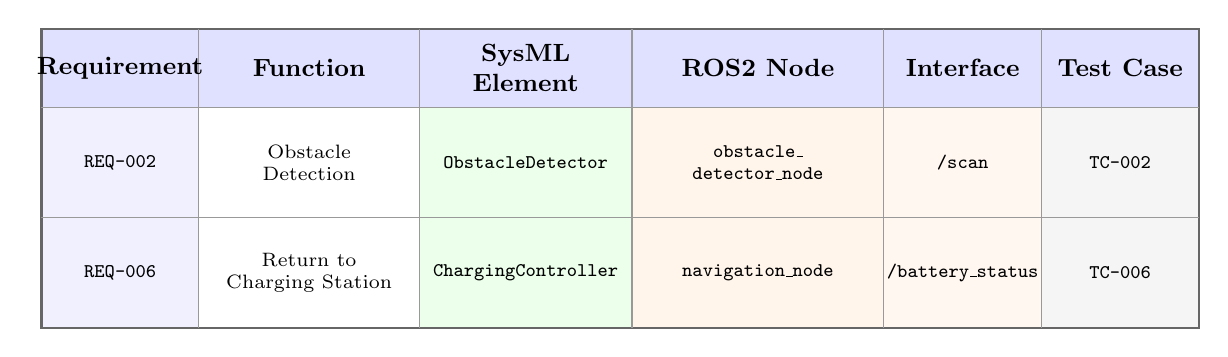
\begin{tikzpicture}[
    every node/.style={font=\small},
    x=1cm, y=1cm
]

% --- column boundaries (x) and row boundaries (y) in cm ---
% Columns: Requirement | Function | SysML system element | ROS2 node | Interface | Test case
% x0=0, x1=2.0, x2=4.8, x3=7.5, x4=10.7, x5=12.7, x6=14.7
% Rows (from top): y0=3.8 (header top), y1=2.8 (header bottom / row 1 top),
%                   y2=1.4 (row 1 bottom / row 2 top), y3=0 (row 2 bottom)

% --- column background for data rows (y3 to y1) ---
\fill[blue!6]   (0,0)    rectangle (2.0,2.8);
\fill[white]    (2.0,0)  rectangle (4.8,2.8);
\fill[green!8]  (4.8,0)  rectangle (7.5,2.8);
\fill[orange!8] (7.5,0)  rectangle (10.7,2.8);
\fill[orange!6] (10.7,0) rectangle (12.7,2.8);
\fill[black!4]  (12.7,0) rectangle (14.7,2.8);

% --- shade the header row on top ---
\fill[blue!12] (0,2.8) rectangle (14.7,3.8);

% --- grid lines: outer frame ---
\draw[black!60, thick] (0,0) rectangle (14.7,3.8);

% --- grid lines: vertical column separators ---
\draw[black!40] (2.0,0)  -- (2.0,3.8);
\draw[black!40] (4.8,0)  -- (4.8,3.8);
\draw[black!40] (7.5,0)  -- (7.5,3.8);
\draw[black!40] (10.7,0) -- (10.7,3.8);
\draw[black!40] (12.7,0) -- (12.7,3.8);

% --- grid lines: horizontal row separators ---
\draw[black!40] (0,1.4) -- (14.7,1.4);
\draw[black!40] (0,2.8) -- (14.7,2.8);

% --- header text ---
\node[font=\small\bfseries] at (1.0,3.3)  {Requirement};
\node[font=\small\bfseries] at (3.4,3.3)  {Function};
\node[font=\small\bfseries, align=center] at (6.15,3.3) {SysML\\Element};
\node[font=\small\bfseries] at (9.1,3.3)  {ROS2 Node};
\node[font=\small\bfseries] at (11.7,3.3) {Interface};
\node[font=\small\bfseries] at (13.7,3.3) {Test Case};

% --- row 1: REQ-002 ---
\node[font=\scriptsize] at (1.0,2.1)  {\texttt{REQ-002}};
\node[font=\scriptsize, align=center] at (3.4,2.1)  {Obstacle\\Detection};
\node[font=\scriptsize] at (6.15,2.1) {\texttt{ObstacleDetector}};
\node[font=\scriptsize, align=center] at (9.1,2.1)  {\texttt{obstacle\_}\\\texttt{detector\_node}};
\node[font=\scriptsize] at (11.7,2.1) {\texttt{/scan}};
\node[font=\scriptsize] at (13.7,2.1) {\texttt{TC-002}};

% --- row 2: REQ-006 ---
\node[font=\scriptsize] at (1.0,0.7)  {\texttt{REQ-006}};
\node[font=\scriptsize, align=center] at (3.4,0.7)  {Return to\\Charging Station};
\node[font=\scriptsize] at (6.15,0.7) {\texttt{ChargingController}};
\node[font=\scriptsize] at (9.1,0.7)  {\texttt{navigation\_node}};
\node[font=\scriptsize] at (11.7,0.7) {\texttt{/battery\_status}};
\node[font=\scriptsize] at (13.7,0.7) {\texttt{TC-006}};

\end{tikzpicture}

}
  \caption{Excerpt from a traceability matrix: each row connects a requirement, through a function, system element, and ROS2 node, to a test case.}
  \label{fig:kap20-traceability-matrix}
\end{figure}

\section{Change Management}
Changes should be assessed deliberately. A simple process:

\begin{enumerate}
    \item Describe the change request.
    \item Identify the affected requirements.
    \item Determine the affected architecture parts and interfaces.
    \item Check the affected tests.
    \item Assess effort and risk.
    \item Document the decision.
\end{enumerate}

You can walk through this process concretely using the speed increase from the previous section: the change request (a higher maximum speed) reveals the affected safety requirements and the braking-distance model, the stopping-distance tests must be adjusted, and only after assessing effort and risk is the decision documented. In larger projects, a dedicated approval body, the Change Control Board (CCB), often makes this decision; for a beginner project, a simple, documented decision is usually enough.

Figure~\ref{fig:kap20-aenderungsmanagement-ablauf} shows this process, including the decision to approve or reject the change.

\begin{figure}[H]
  \centering
  \adjustbox{max width=\linewidth,max totalheight=0.6\textheight}{% =====================================================================
% Figure: Change management process
% Matches Chapter 20, section "Change Management"
%
% Used in the book, e.g. in chapters_en/20_traceability.tex:
%
%   \begin{figure}[H]
%     \centering
%     % =====================================================================
% Figure: Change management process
% Matches Chapter 20, section "Change Management"
%
% Used in the book, e.g. in chapters_en/20_traceability.tex:
%
%   \begin{figure}[H]
%     \centering
%     \input{figures_en/fig_kap20_aenderungsmanagement_ablauf}
%     \caption{The change management process, from describing the
%       change request to the documented decision.}
%     \label{fig:kap20-aenderungsmanagement-ablauf}
%   \end{figure}
%
% Required packages (already loaded in main_en.tex): tikz
% Required TikZ libraries: positioning, arrows.meta, shadows, calc
% =====================================================================

\resizebox{\textwidth}{!}{\input{figures_en/fig_kap20_aenderungsmanagement_ablauf.tikz}}

%     \caption{The change management process, from describing the
%       change request to the documented decision.}
%     \label{fig:kap20-aenderungsmanagement-ablauf}
%   \end{figure}
%
% Required packages (already loaded in main_en.tex): tikz
% Required TikZ libraries: positioning, arrows.meta, shadows, calc
% =====================================================================

\resizebox{\textwidth}{!}{\begin{tikzpicture}[
    scale=0.71, transform shape,
    every node/.style={font=\small},
    proc/.style={
        rectangle, rounded corners=2pt, draw=black!60, thick,
        minimum width=34mm, minimum height=12mm,
        align=center, fill=black!4, drop shadow
    },
    decide/.style={
        rectangle, minimum width=32mm, minimum height=22mm,
        align=center, inner sep=1pt
    },
    okbox/.style={
        rectangle, rounded corners=2pt, draw=green!40!black, thick,
        minimum width=34mm, minimum height=12mm,
        align=center, fill=green!15, drop shadow
    },
    endbox/.style={
        rectangle, rounded corners=2pt, draw=black!50, thick,
        minimum width=34mm, minimum height=12mm,
        align=center, fill=black!6, drop shadow
    },
    flow/.style={-{Stealth[length=2.2mm]}, thick, black!60},
    lbl/.style={font=\small, fill=white, inner sep=1pt}
]

% --- row 1 (left to right) ---
\node[proc] (s1) at (0, 9)   {(1) Describe\\change request};
\node[proc] (s2) at (4.6, 9) {(2) Identify\\affected\\requirements};
\node[proc] (s3) at (9.2, 9) {(3) Determine affected\\architecture parts/\\interfaces};

% --- row 2 (right to left, S-shaped flow) ---
\node[proc] (s4) at (9.2, 5.2) {(4) Check affected\\tests};
\node[proc] (s5) at (4.6, 5.2) {(5) Assess effort/\\risk};
\node[proc] (s6) at (0, 5.2)   {(6) Document\\decision};

% --- decision: diamond drawn manually (no shapes.geometric library needed) ---
% Corner points of the diamond match the anchor points (.north/.east/.south/.west)
% of the invisible "dec" node with the same width/height.
\filldraw[fill=black!4, draw=black!70, thick] (0, 2.1) -- (1.6, 1.0) -- (0, -0.1) -- (-1.6, 1.0) -- cycle;
\node[decide] (dec) at (0, 1.0) {Approved?};

% --- outcome boxes ---
\node[okbox]  (ok)  at (5.0, 1.0)  {Implement/\\change model};
\node[endbox] (end) at (0, -3.2)   {Document\\\& end};

% --- flow row 1 ---
\draw[flow] (s1) -- (s2);
\draw[flow] (s2) -- (s3);

% --- transition row1 -> row2 ---
\draw[flow] (s3.south) -- (s4.north);

% --- flow row 2 ---
\draw[flow] (s4) -- (s5);
\draw[flow] (s5) -- (s6);

% --- to the decision ---
\draw[flow] (s6.south) -- (dec.north);

% --- yes / no ---
\draw[flow] (dec.east) -- node[lbl, midway]{Yes} (ok.west);
\draw[flow] (dec.south) -- node[lbl, midway]{No} (end.north);

% --- optional loop back (dashed) ---
\draw[dashed, thick, black!50, -{Stealth[length=2mm]}]
    (end.west) -- ++(-2.2,0) -- ++(0, 12.2) -- (s1.west)
    node[lbl, pos=0.55, left]{possible new change request};

\end{tikzpicture}
}
}
  \caption{The change management process, from describing the change request to the documented decision.}
  \label{fig:kap20-aenderungsmanagement-ablauf}
\end{figure}

\section{Common Mistakes}
Traceability is often built too late. Then it becomes tedious. It is better to maintain relationships step by step as you model. Another mistake is building too much traceability with no real benefit. Link above all the elements that matter for decisions, changes, and tests.

\section{A Pragmatic Scope}
Traceability can grow very large very quickly. For a beginner project, keep it deliberately limited. At first, focus on the main requirements, main blocks, central interfaces, ROS2 nodes, and test cases.

A good starting rule: every main requirement should have at least one relationship to a satisfying model element and one proof. Every safety-relevant requirement should also be linked to its affected interfaces and failure cases.

For the indoor robot, the following are especially worth tracing:

\begin{itemize}
    \item obstacle detection
    \item person detection
    \item returning to the charging station
    \item a safe stop
    \item battery-level monitoring
    \item status and error messages
\end{itemize}

These chains deliver a lot of value without immediately overloading the model.

\subsection{Example: Changing the Return Strategy}
The in-depth battery example shows a concrete change compared to the simple battery threshold: REQ-005 and REQ-006 are made more precise by BM-01 through BM-13 (Section~\ref{sec:bm-anforderungen}). The procedure in Section~\ref{sec:bm-ablauf}, the energy balance in Section~\ref{sec:bm-energie}, and the tests in Section~\ref{sec:bm-tests} together form the detailed design.

One example chain:
\begin{quote}
REQ-006: Return to the charging station\\
BM-05: Pause the order if the estimate is not reliable\\
Functions: assess estimate validity and safeguard the return\\
Intended responsibility: battery management and navigation\\
Information needed: energy demand, route data, and their validity\\
T-03/T-04: map missing, or return path unknown
\end{quote}

Here, the responsibility is an architecture assignment in the design. It does not yet correspond to a concrete SysML relationship or ROS2 implementation that has been created or checked. In particular, the existing battery monitor alone does not implement the new return safeguard.

If the recorded route is later replaced by a different return strategy, this affects at least BM-01, BM-06, BM-07, and BM-11, the interfaces for route data, the return decision, and T-03, T-06, and T-11. Before such a change, you must also check the energy assumptions and any other affected tests. The status of every relationship must show clearly whether it is only planned, implemented, or backed by a passed proof.

\section{Summary}
Traceability connects requirements, architecture, implementation, and tests. It makes change manageable and helps you find gaps in the model. For the indoor robot, it is especially valuable because sensing, software, energy, and safety are closely linked.

\section{Review Questions}
\begin{enumerate}
    \item What does traceability mean?
    \item Why does traceability matter in MBSE?
    \item What is impact analysis?
    \item What elements does a traceability chain contain?
    \item Why should traceability be built early?
    \item Which elements would a higher robot speed affect?
\end{enumerate}

\section{Exercises}
\begin{uebungbox}
\textbf{Exercise 1: Traceability chain}\\
Choose a requirement and build a complete traceability chain down to a test case.
\end{uebungbox}

\begin{uebungbox}
\textbf{Exercise 2: Impact analysis}\\
Analyze this change: the camera is replaced with a depth camera. Which requirements, system parts, interfaces, ROS2 nodes, and tests are affected?
\end{uebungbox}

\section{Further Reading}
Traceability is a core topic in MBSE and requirements engineering. SysML v2 offers relationships such as \texttt{satisfy}, \texttt{verify}, \texttt{derive}, and \texttt{trace} for this purpose \cite{sysmlv2pilot}.

\chapter{Capstone Project}

\begin{lernziele}
After this chapter, you can structure a small but complete MBSE project for a ROS2 robot. You can connect requirements, structure, behavior, interfaces, ROS2 mapping, tests, and traceability into one coherent model.
\end{lernziele}

\section{Introduction}
The capstone project ties the previous chapters together. You build a complete model of the autonomous indoor robot. It does not need to be industrially perfect. But it must show that requirements, architecture, and tests fit together.

\section{The Task}
Build a complete model of the autonomous indoor robot. The model must include requirements, structure, behavior, interfaces, ROS2 mapping, and tests.

\section{What the Model Must Contain}
The model should contain the following:

\begin{itemize}
    \item a context description
    \item a stakeholder list
    \item at least ten requirements
    \item a requirement diagram
    \item a BDD with the main systems (see Chapter 8)
    \item an IBD for perception or navigation (see Chapter 9)
    \item an activity diagram for target navigation
    \item a state diagram for operating modes
    \item an interface table
    \item a ROS2 mapping table
    \item at least five test cases
    \item a traceability matrix
\end{itemize}

Figure~\ref{fig:kap21-checkliste-abschlussmodell} summarizes these items as a checklist you can use to review your model before submitting it.

\begin{figure}[H]
  \centering
  \adjustbox{max width=\linewidth,max totalheight=0.6\textheight}{% =====================================================================
% Figure: Checklist: contents of the capstone model
% Matches Chapter 21, section "What the Model Must Contain"
%
% Used in the book, e.g. in chapters_en/21_abschlussprojekt.tex:
%
%   \begin{figure}[H]
%     \centering
%     % =====================================================================
% Figure: Checklist: contents of the capstone model
% Matches Chapter 21, section "What the Model Must Contain"
%
% Used in the book, e.g. in chapters_en/21_abschlussprojekt.tex:
%
%   \begin{figure}[H]
%     \centering
%     \input{figures_en/fig_kap21_checkliste_abschlussmodell}
%     \caption{A checklist with the twelve items the capstone model
%       should contain.}
%     \label{fig:kap21-checkliste-abschlussmodell}
%   \end{figure}
%
% Required packages (already loaded in main_en.tex): tikz
% Required TikZ libraries: positioning, arrows.meta, shadows, calc
% =====================================================================

\input{figures_en/fig_kap21_checkliste_abschlussmodell.tikz}

%     \caption{A checklist with the twelve items the capstone model
%       should contain.}
%     \label{fig:kap21-checkliste-abschlussmodell}
%   \end{figure}
%
% Required packages (already loaded in main_en.tex): tikz
% Required TikZ libraries: positioning, arrows.meta, shadows, calc
% =====================================================================

\begin{tikzpicture}[
    every node/.style={font=\small},
    box/.style={draw=black!70, thick, minimum width=2mm, minimum height=2mm, inner sep=0pt}
]

% --- checkboxes and text, line by line ---
\node[box] (cb1)  at (0, 0)     {};
\node[right=2mm of cb1,  font=\small, align=left] {Context description};

\node[box] (cb2)  at (0, -0.95) {};
\node[right=2mm of cb2,  font=\small, align=left] {Stakeholder list};

\node[box] (cb3)  at (0, -1.90) {};
\node[right=2mm of cb3,  font=\small, align=left] {At least ten requirements};

\node[box] (cb4)  at (0, -2.85) {};
\node[right=2mm of cb4,  font=\small, align=left] {Requirement diagram};

\node[box] (cb5)  at (0, -3.80) {};
\node[right=2mm of cb5,  font=\small, align=left] {BDD with the main systems};

\node[box] (cb6)  at (0, -4.75) {};
\node[right=2mm of cb6,  font=\small, align=left] {IBD for one subsystem (e.g. perception or navigation)};

\node[box] (cb7)  at (0, -5.70) {};
\node[right=2mm of cb7,  font=\small, align=left] {Activity diagram for target navigation};

\node[box] (cb8)  at (0, -6.65) {};
\node[right=2mm of cb8,  font=\small, align=left] {State diagram for operating modes};

\node[box] (cb9)  at (0, -7.60) {};
\node[right=2mm of cb9,  font=\small, align=left] {Interface table};

\node[box] (cb10) at (0, -8.55) {};
\node[right=2mm of cb10, font=\small, align=left] {ROS2 mapping table};

\node[box] (cb11) at (0, -9.50) {};
\node[right=2mm of cb11, font=\small, align=left] {At least five test cases};

\node[box] (cb12) at (0, -10.45) {};
\node[right=2mm of cb12, font=\small, align=left] {Traceability matrix};

\end{tikzpicture}

}
  \caption{A checklist with the twelve items the capstone model should contain.}
  \label{fig:kap21-checkliste-abschlussmodell}
\end{figure}

\section{Recommended Approach}
\begin{enumerate}
    \item State the system goal and the system boundary.
    \item Gather stakeholders and their needs.
    \item Write and number the requirements.
    \item Model the main structure in a BDD.
    \item Show one important subsystem in an IBD.
    \item Describe behavior with an activity diagram and a state diagram.
    \item Document interfaces in a table.
    \item Map SysML elements to ROS2 elements.
    \item Create test cases and link them to requirements.
    \item Check the traceability matrix.
\end{enumerate}

Figure~\ref{fig:kap21-projektfahrplan} summarizes these ten steps as a roadmap in four phases.

\begin{figure}[H]
  \centering
  \adjustbox{max width=\linewidth,max totalheight=0.6\textheight}{% =====================================================================
% Figure: Capstone project roadmap
% Matches Chapter 21, section "Recommended Approach"
%
% Used in the book, e.g. in chapters_en/21_abschlussprojekt.tex:
%
%   \begin{figure}[H]
%     \centering
%     % =====================================================================
% Figure: Capstone project roadmap
% Matches Chapter 21, section "Recommended Approach"
%
% Used in the book, e.g. in chapters_en/21_abschlussprojekt.tex:
%
%   \begin{figure}[H]
%     \centering
%     \input{figures_en/fig_kap21_projektfahrplan}
%     \caption{Ten steps of the capstone project, grouped into four
%       phases from requirements to verification.}
%     \label{fig:kap21-projektfahrplan}
%   \end{figure}
%
% Required packages (already loaded in main_en.tex): tikz
% Required TikZ libraries: positioning, arrows.meta, shadows, calc, backgrounds
% =====================================================================

\input{figures_en/fig_kap21_projektfahrplan.tikz}

%     \caption{Ten steps of the capstone project, grouped into four
%       phases from requirements to verification.}
%     \label{fig:kap21-projektfahrplan}
%   \end{figure}
%
% Required packages (already loaded in main_en.tex): tikz
% Required TikZ libraries: positioning, arrows.meta, shadows, calc, backgrounds
% =====================================================================

\begin{tikzpicture}[
    every node/.style={font=\small},
    reqstep/.style={
        rectangle, rounded corners=2pt, draw=black!70, thick,
        minimum width=34mm, minimum height=13mm,
        align=center, fill=blue!12, drop shadow
    },
    archstep/.style={
        rectangle, rounded corners=2pt, draw=green!40!black, thick,
        minimum width=34mm, minimum height=13mm,
        align=center, fill=green!15, drop shadow
    },
    ifacestep/.style={
        rectangle, rounded corners=2pt, draw=orange!60!black, thick,
        minimum width=34mm, minimum height=13mm,
        align=center, fill=orange!15, drop shadow
    },
    veristep/.style={
        rectangle, rounded corners=2pt, draw=black!50, thick,
        minimum width=34mm, minimum height=13mm,
        align=center, fill=black!6, drop shadow
    },
    flow/.style={-{Stealth[length=2.2mm]}, thick, black!60}
]

% --- Phase 1: Requirements (blue) ---
\node[reqstep] (s1) at (0, 15)   {\textbf{(1)} System goal/\\system boundary};
\node[reqstep] (s2) at (4.4, 15) {\textbf{(2)} Gather\\stakeholders/\\needs};
\node[reqstep] (s3) at (8.8, 15) {\textbf{(3)} Write/number\\requirements};

% --- Phase 2: Architecture and behavior (green) ---
\node[archstep] (s4) at (0, 10.5)   {\textbf{(4)} Model main\\structure\\in BDD};
\node[archstep] (s5) at (4.4, 10.5) {\textbf{(5)} Show\\subsystem\\in IBD};
\node[archstep] (s6) at (8.8, 10.5) {\textbf{(6)} Activity/\\state\\diagram};

% --- Phase 3: Interfaces/implementation (orange) ---
\node[ifacestep] (s7) at (0, 6)   {\textbf{(7)} Document\\interfaces};
\node[ifacestep] (s8) at (4.4, 6) {\textbf{(8)} ROS2 mapping};

% --- Phase 4: Verification (gray) ---
\node[veristep] (s9)  at (0, 1.5)   {\textbf{(9)} Create/link\\test cases};
\node[veristep] (s10) at (4.4, 1.5) {\textbf{(10)} Check\\traceability matrix};

% --- flow within each phase ---
\draw[flow] (s1) -- (s2);
\draw[flow] (s2) -- (s3);
\draw[flow] (s4) -- (s5);
\draw[flow] (s5) -- (s6);
\draw[flow] (s7) -- (s8);
\draw[flow] (s9) -- (s10);

% --- transitions between phases (elbow connectors) ---
\draw[flow] (s3.south) -- ++(0,-1.2) -| (s4.north);
\draw[flow] (s6.south) -- ++(0,-1.0) -| (s7.north);
\draw[flow] (s8.south) -- ++(0,-1.0) -| (s9.north);

% --- background frame per phase ---
\begin{scope}[on background layer]
    \draw[dashed, thick, blue!50, rounded corners]
        ($(s1.north west)+(-4mm,6mm)$) rectangle ($(s3.south east)+(4mm,-4mm)$);
    \node[font=\small\bfseries, blue!50!black] at ($(s2.north)+(0,10mm)$) {Requirements};

    \draw[dashed, thick, green!40!black, rounded corners]
        ($(s4.north west)+(-4mm,6mm)$) rectangle ($(s6.south east)+(4mm,-4mm)$);
    \node[font=\small\bfseries, green!40!black] at ($(s5.north)+(0,10mm)$) {Architecture / Behavior};

    \draw[dashed, thick, orange!60!black, rounded corners]
        ($(s7.north west)+(-4mm,6mm)$) rectangle ($(s8.south east)+(4mm,-4mm)$);
    \node[font=\small\bfseries, orange!60!black] at ($(s7.north east)+(0,10mm)$) {Interfaces/Implementation};

    \draw[dashed, thick, black!50, rounded corners]
        ($(s9.north west)+(-4mm,6mm)$) rectangle ($(s10.south east)+(4mm,-4mm)$);
    \node[font=\small\bfseries, black!50] at ($(s9.north east)+(0,10mm)$) {Verification};
\end{scope}

\end{tikzpicture}

}
  \caption{Ten steps of the capstone project, grouped into four phases from requirements to verification.}
  \label{fig:kap21-projektfahrplan}
\end{figure}

\section{Evaluation Criteria}
A good model is clear, consistent, and easy to follow. It does not need to be maximally detailed. It must show that the architecture was derived from the requirements.

Important criteria:

\begin{itemize}
    \item a clear system boundary
    \item understandable requirements
    \item consistent names
    \item a sensible structure
    \item documented interfaces
    \item a traceable ROS2 mapping
    \item test cases with \texttt{verify} relationships
    \item no isolated, unexplained diagrams
\end{itemize}

These criteria also work as a short checklist you can go through, point by point, before submitting your model.

\section{Going Further}
If you want to go further, add a simple ROS2 simulation. You can add a simulated battery node, a status node, and a dummy object detector, based on the node examples from Chapter 17. What matters is that the implementation stays tied back to the model. Chapter 22 shows, with Gazebo, one way to extend such a simulation further.

\section{Common Project Pitfalls}
\subsection{Too Much Detail}
A capstone model does not need to cover every detail. The focus is the end-to-end connection.

\subsection{No Traceability}
If requirements, system parts, and tests are not connected, the project stays a collection of separate diagrams.

\subsection{An Unclear Submission}
Document which diagrams and tables are part of your submission. A start page in the model helps.

\section{Recommended Final Documentation}
Alongside the model, write a short final write-up. It does not need to be long, but it should guide the reader through the model. A sensible structure:

\begin{itemize}
    \item the system's goal and scope
    \item the key stakeholders
    \item the key requirements
    \item an architecture overview
    \item the central interfaces
    \item the ROS2 mapping
    \item the test and verification concept
    \item open assumptions and limits
\end{itemize}

This write-up is not a repeat of every diagram. It explains how the diagrams connect. That is what turns the model into a traceable project result.

\section{Summary}
The capstone project shows whether you have understood the core idea of this book: going from a problem, through requirements and SysML modeling, to a ROS2-oriented architecture and verification. The autonomous indoor robot serves as the running, hands-on example throughout.

\section{Review Questions}
\begin{enumerate}
    \item What must the capstone model contain?
    \item Why does a traceability matrix matter?
    \item What sets a good model apart from a collection of diagrams?
    \item Which evaluation criteria matter most?
    \item How can you usefully add a ROS2 extension?
\end{enumerate}

\section{Exercises}
\begin{uebungbox}
\textbf{Exercise 1: Traceability matrix}\\
Build a traceability matrix with the columns requirement, system element (\texttt{part def}), ROS2 node, and test case.
\end{uebungbox}

\begin{uebungbox}
\textbf{Exercise 2: Model review}\\
Review your model: Are there requirements with no test? System parts with no purpose? Interfaces with no data type? Note at least five improvements.
\end{uebungbox}

\section{Further Reading}
For the capstone project, revisit the previous chapters along with the SysML and ROS2 sources \cite{delligatti2014,friedenthal2014,ros2docs}.

\chapter{Outlook}

\begin{lernziele}
After this chapter, you know sensible next steps for going deeper. You can place the topics that follow this beginner's book: advanced SysML modeling, SysML v2, ROS2 in practice, simulation, safety engineering, machine learning, and professional application.
\end{lernziele}

\section{Introduction}
This book offers a starting point. It shows how SysML v2, MBSE, and ROS2 work together, using an autonomous indoor robot as the example. After this start, there are many paths to go deeper. This chapter maps out the most important next steps. Figure~\ref{fig:kap22-vertiefungs-roadmap} gives an overview of the six topic areas covered in the following sections.

\begin{figure}[H]
  \centering
  \adjustbox{max width=\linewidth,max totalheight=0.6\textheight}{% =====================================================================
% Figure: Roadmap for going deeper after this book
% Matches Chapter 22, introduction / "Possible Next Projects"
%
% Used in the book, e.g. in chapters_en/22_ausblick.tex:
%
%   \begin{figure}[H]
%     \centering
%     % =====================================================================
% Figure: Roadmap for going deeper after this book
% Matches Chapter 22, introduction / "Possible Next Projects"
%
% Used in the book, e.g. in chapters_en/22_ausblick.tex:
%
%   \begin{figure}[H]
%     \centering
%     \input{figures_en/fig_kap22_vertiefungs_roadmap}
%     \caption{Possible directions to go deeper after this book,
%       grouped into six topic areas with selected subtopics.}
%     \label{fig:kap22-vertiefungs-roadmap}
%   \end{figure}
%
% Required packages (already loaded in main_en.tex): tikz
% Required TikZ libraries: positioning, arrows.meta, shadows, calc
% =====================================================================

\resizebox{\textwidth}{!}{\input{figures_en/fig_kap22_vertiefungs_roadmap.tikz}}

%     \caption{Possible directions to go deeper after this book,
%       grouped into six topic areas with selected subtopics.}
%     \label{fig:kap22-vertiefungs-roadmap}
%   \end{figure}
%
% Required packages (already loaded in main_en.tex): tikz
% Required TikZ libraries: positioning, arrows.meta, shadows, calc
% =====================================================================

\resizebox{\textwidth}{!}{\begin{tikzpicture}[
    scale=0.75, transform shape,
    every node/.style={font=\small},
    center/.style={
        rectangle, rounded corners=2pt, draw=black!70, thick,
        minimum width=34mm, minimum height=13mm,
        align=center, fill=blue!12, drop shadow
    },
    sysmlnode/.style={
        rectangle, rounded corners=2pt, draw=green!40!black, thick,
        minimum width=28mm, minimum height=10mm,
        align=center, fill=green!15, drop shadow
    },
    rosnode/.style={
        rectangle, rounded corners=2pt, draw=orange!60!black, thick,
        minimum width=28mm, minimum height=10mm,
        align=center, fill=orange!15, drop shadow
    },
    mlnode/.style={
        rectangle, rounded corners=2pt, draw=blue!40!black, thick,
        minimum width=28mm, minimum height=10mm,
        align=center, fill=blue!6, drop shadow
    },
    neutralnode/.style={
        rectangle, rounded corners=2pt, draw=black!50, thick,
        minimum width=28mm, minimum height=10mm,
        align=center, fill=black!6, drop shadow
    },
    subnode/.style={
        rectangle, rounded corners=1.5pt, draw=black!40, thick,
        minimum width=24mm, minimum height=8mm,
        align=center, font=\footnotesize, fill=white, drop shadow
    },
    mainedge/.style={thick, black!50},
    subedge/.style={thin, black!35}
]

% --- center ---
\node[center] (center) at (0,0) {After\\This Start};

% --- main branches ---
\node[sysmlnode]   (sysml)   at (90:4)   {SysML in\\Depth};
\node[sysmlnode]   (sysmlv2) at (30:4)   {SysML v2};
\node[rosnode]     (ros)     at (-30:4)  {ROS2 in\\Depth};
\node[neutralnode] (sim)     at (-90:4)  {Simulation};
\node[neutralnode] (safety)  at (-150:4) {Safety\\Engineering};
\node[mlnode]      (ml)      at (150:4)  {Machine\\Learning};

% --- center -> main branches ---
\draw[mainedge] (center) -- (sysml);
\draw[mainedge] (center) -- (sysmlv2);
\draw[mainedge] (center) -- (ros);
\draw[mainedge] (center) -- (sim);
\draw[mainedge] (center) -- (safety);
\draw[mainedge] (center) -- (ml);

% --- sub-branches: ROS2 in depth ---
\node[subnode] (nav2)   at (-55:7.3) {Navigation2};
\node[subnode] (tf2)    at (-30:7.3) {TF2};
\node[subnode] (life)   at (-5:7.3)  {Lifecycle\\Nodes};
\draw[subedge] (ros) -- (nav2);
\draw[subedge] (ros) -- (tf2);
\draw[subedge] (ros) -- (life);

% --- sub-branches: safety engineering ---
\node[subnode] (fmea) at (-168:7.3) {FMEA};
\node[subnode] (gefahr) at (-132:7.3) {Hazard\\Analyses};
\draw[subedge] (safety) -- (fmea);
\draw[subedge] (safety) -- (gefahr);

% --- sub-branches: machine learning ---
\node[subnode] (train) at (132:7.3) {Training\\Data};
\node[subnode] (valid) at (168:7.3) {Validation\\Datasets};
\draw[subedge] (ml) -- (train);
\draw[subedge] (ml) -- (valid);

\end{tikzpicture}
}
}
  \caption{Possible directions to go deeper after this book, grouped into six topic areas with selected subtopics.}
  \label{fig:kap22-vertiefungs-roadmap}
\end{figure}

\section{Going Deeper into SysML}
After this start, you should learn SysML in more depth. These topics matter especially:

\begin{itemize}
    \item clean model organization
    \item reuse of model elements
    \item variant modeling
    \item interface concepts
    \item formal requirements
    \item parametrics and engineering analysis
    \item model review and model quality
\end{itemize}

\section{SysML v2}
SysML v2 modernizes the language and brings more precise textual and graphical modeling. For beginners, SysML v1.x is still widespread, but SysML v2 will matter more in the long run.

Important topics for later:

\begin{itemize}
    \item textual modeling
    \item more precise semantics
    \item better tool support
    \item migrating existing models
    \item connecting to modern MBSE methods
\end{itemize}

\section{Going Deeper into ROS2}
For robotics, the following ROS2 topics are important next steps:

\begin{itemize}
    \item Navigation2 (the navigation stack for path planning and obstacle avoidance)
    \item TF2 (a library for managing coordinate transforms)
    \item lifecycle nodes (nodes with defined, managed state transitions)
    \item launch files
    \item parameters
    \item rosbag (a tool for recording and replaying messages)
    \item simulation
    \item testing with launch testing
\end{itemize}

\section{Simulation}
Gazebo and other simulators let you test without real hardware. This is especially valuable when you want to try out algorithms quickly. Simulation can help you check navigation, sensing, obstacles, and failure cases early.

\section{Safety Engineering}
As soon as robots interact with people in real environments, safety questions become important. At that point, simple function models are no longer enough. You must account for risk analyses, safety requirements, FMEA (Failure Mode and Effects Analysis), hazard analyses, and standards. For a service robot like the indoor robot, for example, the standard ISO 13482 for personal care robots is relevant.

\section{Going Deeper into Machine Learning}
ML integration (Machine Learning) does not end once you load a model. Important areas to deepen:

\begin{itemize}
    \item training data
    \item validation datasets
    \item misclassifications
    \item runtime optimization
    \item edge AI hardware
    \item monitoring in operation
    \item handling uncertainty
\end{itemize}

\section{Professional Relevance}
The combination of systems engineering, SysML, ROS2, and AI matters in robotics, automotive, industrial automation, and research. If you understand this connection, you can mediate between architecture, software, and tests. This cross-cutting skill is valuable in many projects.

\section{Possible Next Projects}
\begin{itemize}
    \item a SysML v2 modeling workshop with a complete model build
    \item a small ROS2 workspace with simulated nodes
    \item a Navigation2 demo in simulation
    \item an object detection node with an example model
    \item a SysML v2 comparison chapter
    \item full traceability from requirements to test code
\end{itemize}

\section{From a Learning Project to a Real Project}
The most important step after this book is moving from a didactic model to a real project. In a real project, requirements become more contradictory, interfaces become more technical, and tests become more demanding. Organizational topics also appear: versioning, reviews, responsibilities, change management, and acceptance. Figure~\ref{fig:kap22-lernprojekt-vs-echtes-projekt} contrasts this transition.

\begin{figure}[H]
  \centering
  \adjustbox{max width=\linewidth,max totalheight=0.6\textheight}{% =====================================================================
% Figure: From a learning project to a real project
% Matches Chapter 22, section "From a Learning Project to a Real Project"
%
% Used in the book, e.g. in chapters_en/22_ausblick.tex:
%
%   \begin{figure}[H]
%     \centering
%     % =====================================================================
% Figure: From a learning project to a real project
% Matches Chapter 22, section "From a Learning Project to a Real Project"
%
% Used in the book, e.g. in chapters_en/22_ausblick.tex:
%
%   \begin{figure}[H]
%     \centering
%     \input{figures_en/fig_kap22_lernprojekt_vs_echtes_projekt}
%     \caption{The move from a learning project to a real project
%       brings more complex requirements and interfaces, plus new
%       organizational topics.}
%     \label{fig:kap22-lernprojekt-vs-echtes-projekt}
%   \end{figure}
%
% Required packages (already loaded in main_en.tex): tikz
% Required TikZ libraries: positioning, arrows.meta, shadows, calc
% =====================================================================

\input{figures_en/fig_kap22_lernprojekt_vs_echtes_projekt.tikz}

%     \caption{The move from a learning project to a real project
%       brings more complex requirements and interfaces, plus new
%       organizational topics.}
%     \label{fig:kap22-lernprojekt-vs-echtes-projekt}
%   \end{figure}
%
% Required packages (already loaded in main_en.tex): tikz
% Required TikZ libraries: positioning, arrows.meta, shadows, calc
% =====================================================================

\begin{tikzpicture}[
    scale=0.9, transform shape,
    every node/.style={font=\small},
    lernbox/.style={
        rectangle, rounded corners=2pt, draw=green!40!black, thick,
        minimum width=55mm, minimum height=32mm,
        align=left, fill=green!10, drop shadow
    },
    echtbox/.style={
        rectangle, rounded corners=2pt, draw=orange!60!black, thick,
        minimum width=55mm, minimum height=32mm,
        align=left, fill=orange!12, drop shadow
    },
    themenbox/.style={
        rectangle, rounded corners=2pt, draw=blue!50!black, thick,
        minimum width=100mm, minimum height=20mm,
        align=left, fill=blue!8, drop shadow
    },
    flow/.style={-{Stealth[length=2.4mm]}, thick, black!60},
    connector/.style={thin, black!40}
]

% --- poles ---
\node[lernbox] (lern) at (0,0) {
    \textbf{Learning Project}\\[2mm]
    \textbullet\ Requirements are clear\\
    \textbullet\ Interfaces are simple\\
    \textbullet\ Tests are manageable
};

\node[echtbox] (echt) at (9,0) {
    \textbf{Real Project}\\[2mm]
    \textbullet\ Requirements conflict\\
    \textbullet\ Interfaces are complex\\
    \textbullet\ Tests are demanding
};

% --- transition ---
\draw[flow] (lern.east) -- node[above, font=\small]{Transition in practice} (echt.west);

% --- new topics ---
\node[themenbox] (themen) at (4.5,-4.8) {
    \textbf{New Topics}\\[1mm]
    \textbullet\ Versioning \quad
    \textbullet\ Reviews \quad
    \textbullet\ Responsibilities\\
    \textbullet\ Change Management \quad
    \textbullet\ Acceptance
};

% --- connection to new topics ---
\draw[connector] (lern.south) -- ++(0,-0.6) -| (themen.north);
\draw[connector] (echt.south) -- ++(0,-0.6) -| (themen.north);

\end{tikzpicture}

}
  \caption{The move from a learning project to a real project brings more complex requirements and interfaces, plus new organizational topics.}
  \label{fig:kap22-lernprojekt-vs-echtes-projekt}
\end{figure}

The learning project gives you a foundation for this. Once you understand how a requirement leads to an architecture, and on to ROS2 nodes and tests, you can apply this thinking to larger systems. The scale grows, but the principle stays the same: understand the problem, build a model, clarify interfaces, derive the implementation, and plan proof.

\section{Summary}
You have made a good start once you can think about requirements, structure, behavior, interfaces, ROS2 architecture, and tests together. The next step is to practice these concepts in tools and code. To practice MBSE, model a small system and link its requirements to design elements and tests.

\section{Review Questions}
\begin{enumerate}
    \item Which SysML topics are worth going deeper into?
    \item Why is SysML v2 becoming more important?
    \item Which ROS2 topics should you learn after this start?
    \item Why is simulation valuable for robotics?
    \item Why does safety engineering matter for robots?
    \item Which professional role can the combination of SysML and ROS2 strengthen?
\end{enumerate}

\section{Exercises}
\begin{uebungbox}
\textbf{Exercise 1: Personal learning plan}\\
Define your personal next learning step: going deeper into SysML, implementing ROS2, building a simulation, or trying out ML integration.
\end{uebungbox}

\begin{uebungbox}
\textbf{Exercise 2: Project idea}\\
Describe a small robotics or automation project of your own where you could apply the methods from this book.
\end{uebungbox}

\section{Further Reading}
To go deeper, see the SysML v2 specification, current tool documentation, the SysML v2 pilot project, and the ROS2 documentation \cite{sysmlv2spec,sysmlv2pilot,ros2docs}. Classic SysML literature \cite{delligatti2014,friedenthal2014} is still useful as background, but you must consciously map it onto SysML v2.


\backmatter
\glsaddall
\printglossary[type=\acronymtype,title=List of Abbreviations]
\printglossary[title=Glossary]
\bibliographystyle{plain}
\bibliography{references_en}

\listoffigures

\printindex
